\documentclass[a4paper,twoside,UTF8]{ctexbook}


%%%%%%%%%%%%%%%%%%%%%%%%%%%%% 字 体 与 版 式 %%%%%%%%%%%%%%%%%%%%%%%%%%%%%%

\usepackage[charter]{mathdesign}
\setCJKmainfont{方正聚珍新仿简体}
\setCJKfamilyfont{hei}{FZYouHeiS}

\usepackage{geometry}
\geometry{
 a4paper,
 total={170mm,257mm},
 left=20mm,
 top=20mm,
 }
\usepackage{fancyhdr} 
\pagestyle{fancy}
\cfoot{\hei 高二物理竞赛}
\fancyfoot[RO,LE]{\bfseries \thepage}

%%%%%%%%%%%%%%%%%%%%%%%%%%%%%%%%%%%%%%%%%%%%%%%%%%%%%%%%%%%%%%%%%%%%%%%%%%%


%%%%%%%%%%%%%%%%%%%%%%%%%%%%%    宏    包    %%%%%%%%%%%%%%%%%%%%%%%%%%%%%%

\usepackage{graphicx}
\usepackage{verbatim}
\usepackage{verse}
\usepackage[colorlinks=true, linkcolor=blue]{hyperref}
\usepackage[squaren]{SIunits}
\usepackage{caption}
\usepackage{CJKfntef}
\usepackage{wrapfig}
\usepackage{float}
\usepackage{array}
\usepackage{xcolor}
\usepackage{mdframed}
\usepackage{lmodern}
\usepackage{upgreek}
\usepackage{amsbsy}
\usepackage{amsmath}
\usepackage{eucal}
\usepackage{enumerate}
\usepackage[T1]{fontenc}
\usepackage[utf8]{inputenc}
\usepackage{lgreek}
\usepackage{textcomp}
\usepackage{booktabs}
\usepackage{multirow}

%%%%%%%%%%%%%%%%%%%%%%%%%%%%%%%%%%%%%%%%%%%%%%%%%%%%%%%%%%%%%%%%%%%%%%%%%%%


%%%%%%%%%%%%%%%%%%%%%%%%%%%%% 命 令 与 环 境 %%%%%%%%%%%%%%%%%%%%%%%%%%%%%%

\renewcommand{\emph}[1]{{\color{red} #1}}
\renewcommand{\arraystretch}{1.5}
\renewcommand{\Omega}{\varOmega}
\renewcommand{\tilde}{\widetilde}
\newcommand{\hei}{\CJKfamily{hei}}
\newcommand{\npg}[1]{\vspace{#1}\newpage}
\newcommand{\bs}[1]{\boldsymbol{#1}}
\newcommand{\sidenote}[1]{\marginpar{#1}}
\newcommand{\pow}[1]{\times 10^{#1}}
\newcommand{\abs}[1]{\left| #1 \right|}
\newcommand{\dgr}{^\circ}
\newcommand{\cdgr}{^\circ \mathrm{C}}
\newcommand{\ap}{\textquotesingle}
\newcommand{\si}[1]{\mathrm{#1}}
\newcommand{\ud}{\textrm{d}}
\newcommand{\uD}{\textrm{D}}
\newcommand{\ue}{{\rm e}}
\newcommand{\ui}{{\rm i}}
\newcommand{\uj}{{\rm j}}
\newcommand{\ke}{\frac{1}{4\pi\varepsilon_0}}
\newcommand{\kb}{\frac{\mu_0}{4\pi}}
\newcommand{\ca}{\raisebox{0.5mm}{------}\,}
\newcommand{\dbar}{\textrm{\dj}}
\newcommand{\permil}{\ensuremath{{\,}^\text{o}\mkern-5mu/\mkern-3mu_\text{oo}}}

%%%%%%%%%%%%%%%%%%%%%%%%%%%%%%%%%%%%%%%%%%%%%%%%%%%%%%%%%%%%%%%%%%%%%%%%%%%%

%\includeonly{chapter/induction}
%\includeonly{chapter/kinematics, chapter/dynamics, chapter/statics, chapter/harmonics, chapter/gravity, chapter/rigidbody, chapter/elasticity, chapter/fluid}
%\includeonly{chapter/thermoI, chapter/thermoII, chapter/maxwell, chapter/liquidsolid, chapter/phasechange, chapter/goptics, chapter/opticals, chapter/opticalp, chapter/electrostatics, chapter/conductordielectric}
%\includeonly{chapter/electrostatics, chapter/conductordielectric, chapter/steadycurrent, chapter/magnetostatics, chapter/induction,  chapter/maxwelle, chapter/accurrent, chapter/relativity, chapter/interference, chapter/diffraction, chapter/photon, chapter/quantum, chapter/scale}


%%%%%%%%%%%%%%%%%%%%%%%%%%%%%%     正    文    %%%%%%%%%%%%%%%%%%%%%%%%%%%%%

\title{\hei \Huge 高二物理竞赛$\bullet$ 热学与几何光学}
\author{学而思}
\date{}


\begin{document}



\frontmatter
\maketitle


\mainmatter
\tableofcontents

% %!TEX root = ../physical-olympics-2.tex
\chapter{序}

\section{说在一切前面}

\begin{altverse}
\centering \large

There are clues everywhere,\\
 all around us.\\
The wrong interpretatation of the clues,\\
 we call our world.\\
---  David Lynch\\
\end{altverse}

现代人的生活,\,变换莫测,\,日新月异.\,不同人用着不同的方式去理解变化背后体现出来的规律.\,优秀的理解方式互相交流与学习,\,学科就从中诞生.\,\emph{物理学}(physics)就是其中的一门学科,\,它是\emph{自然科学}(nature science)的主要构成成分之一.\,今天也许很难找到依据为物理学和自然科学的范围明确划分界限,\,但是物理学秉承了自然科学的一些重要方法论特征,\,是可以帮助我们明显的与其他学科做区分的,\,它们包括:
\begin{itemize}
\item 经验主义.\,把物理学和文学,\,艺术,\,乃至亲缘关系近的数学比对,\,就容易发现后者们的核心在于创新而非做回顾.\,而物理很多时候,\,etc
\item 实验物理.\,
\item 可证伪性.\,
\item 与数学水乳交融:\,描述与诠释.\,
\item 有效预言.\,
\end{itemize}


\section{本书编排}

\section{预备知识}

\subsection{力学}

\subsection{电磁学}

\subsection{热学}

\subsection{光学}

\subsection{近代物理}

\subsection{数学}

% %!TEX root = ../physical-olympics-2.tex
\chapter{运动学}

\section{时空与物质}

物理学,\,从刚开始成为实验性的科学的伽利略时期开始,\,到近半个世纪年来理论物理学家对额外维度的探讨,\,都给予了\emph{时空}(spacetime)最核心的地位.\,牛顿的理论,\,分析力学,\,经典场论,\,相对论这些理论最基本的图像都是时空与\emph{物质}(matter)的分立性.\,时空是装备了一个能体现出物理物理意义的\emph{度量}(metric)的3+1维对象\footnote{数学上有一套严格的说法,\,把这种连续,\,光滑的四维对象称为\emph{伪黎曼流形}(pseudo-Riemannian manifold).}.\,而物质是在每个时空点处的某种结构.\,下面会分别介绍不同物质体系的描述方法.\,在这之前我们来看看不同的时空观:

\subsection{时空观,\,坐标系}
牛顿力学理论体系基于\emph{伽利略时空观}(Galilean spacetime picture),\,也就是\emph{绝对时空观}(absolute spacetime picture).\,在这里空间是三维的平直空间.\,设想一个人站在该空间的某个空间点,\,他的胸前,\,头顶和右手平举的三个方向就是相互垂直的方向.\,如果以自己的臂长为标准长度,\,他能够定义空间中每两个点之间的空间间隔.\,事实上,\,这个人能够以一种正确的方式为每个空间点定义一个坐标,\,那么所有三维空间点的集合与任意两个点之间的距离为:
\[A(x,y,z)\in\mathbb{R}^3 \quad;\quad x,y,z\in\mathbb{R}\]
\[A(x_1,y_1,z_1)\;,\;B(x_2,y_2,z_2)\;:\;l^2=\overline{AB}^2=(x_1-x_2)^2+(y_1-y_2)^2+(z_1-z_2)^2\]

因为空间不同于时间,\,我们为以上数字赋予特殊的物理含义,\,也就是加上\emph{量纲}(dimension).\,如果两点坐标为$(0,0,0)$和$(1,1,1)$,\,那么$l=\sqrt{3}{\rm m}$,\,而不是$l=\sqrt{3}$.\,其单位${\rm m}$一方面表示了这个物理量的属性,\,另一方面指定了某个实际物理体系确定下来的固有长度大小.\,现行的(2018年1月1日,\,下文同)国际单位制对$1{\rm m}$的定义如下\footnote{一方面,\,它依赖于狭义相对论的正确性,\,目前极少理论物理工作者会质疑它.\,另一方面,\,应该要先定义下文的1s,\,再来定义1m.}:
\begin{verse}
1m是光在1/299792458\,s内在真空中行进的距离.
\end{verse}


这就是我们的\emph{三维平直空间}(3-dimensional flat space).\,注意空间点具有物理实际意义,\,它可以脱离坐标系而单独存在.\,事实上坐标系的原点可以建立在空间中的任意点处,\,朝向也可以是任意方向,\,两个空间点之间的距离$l$不会依赖于坐标系的选取,\,但两个点的坐标会因坐标系不同而改变.\,如果我们选取的坐标系总是下述使得两个相距很近的点之间的微元距离公式成立:
\[\ud l^2=\ud x^2+\ud y^2+\ud z^2\]


那么建立的坐标系就是一个\emph{笛卡尔坐标系}(Cartesian coordinate system),\,即\emph{空间直角坐标系}(3D orthogonal coordinate system).\,但是以空间直角坐标系为基础,\,我们又经常建立\emph{球坐标}(spherical coordinate)和\emph{柱坐标}(cylindrical coordinate)系统.\,通常取$x$轴为\emph{幅轴}(azimuth axis),\,点在$x-y$平面上的投影与原点的连线相对$x$轴转过的角度为$\varphi$,\,即\emph{幅角}(azimuth angle).\,而$z$轴为\emph{极轴}(polar axis),\,而点与原点连线与极轴的夹角$\theta$为\emph{极角}(polar angle).\,天文观测用球坐标就很方便,\,它是以描述的空间点到原点之间的距离$r$,\,也称\emph{矢径}(radius),\,和两个描述角位置的极角幅角来构成三个坐标$(r,\theta,\varphi)$的.\,而理论物理里也常用到的柱坐标是以$(\rho,\varphi,z)$为描述空间点的坐标,\,$\rho$是空间点到$z$轴的距离.

\begin{wrapfigure}[14]{o}[-10pt]{7cm}
\vspace{-0.4cm}
\centering
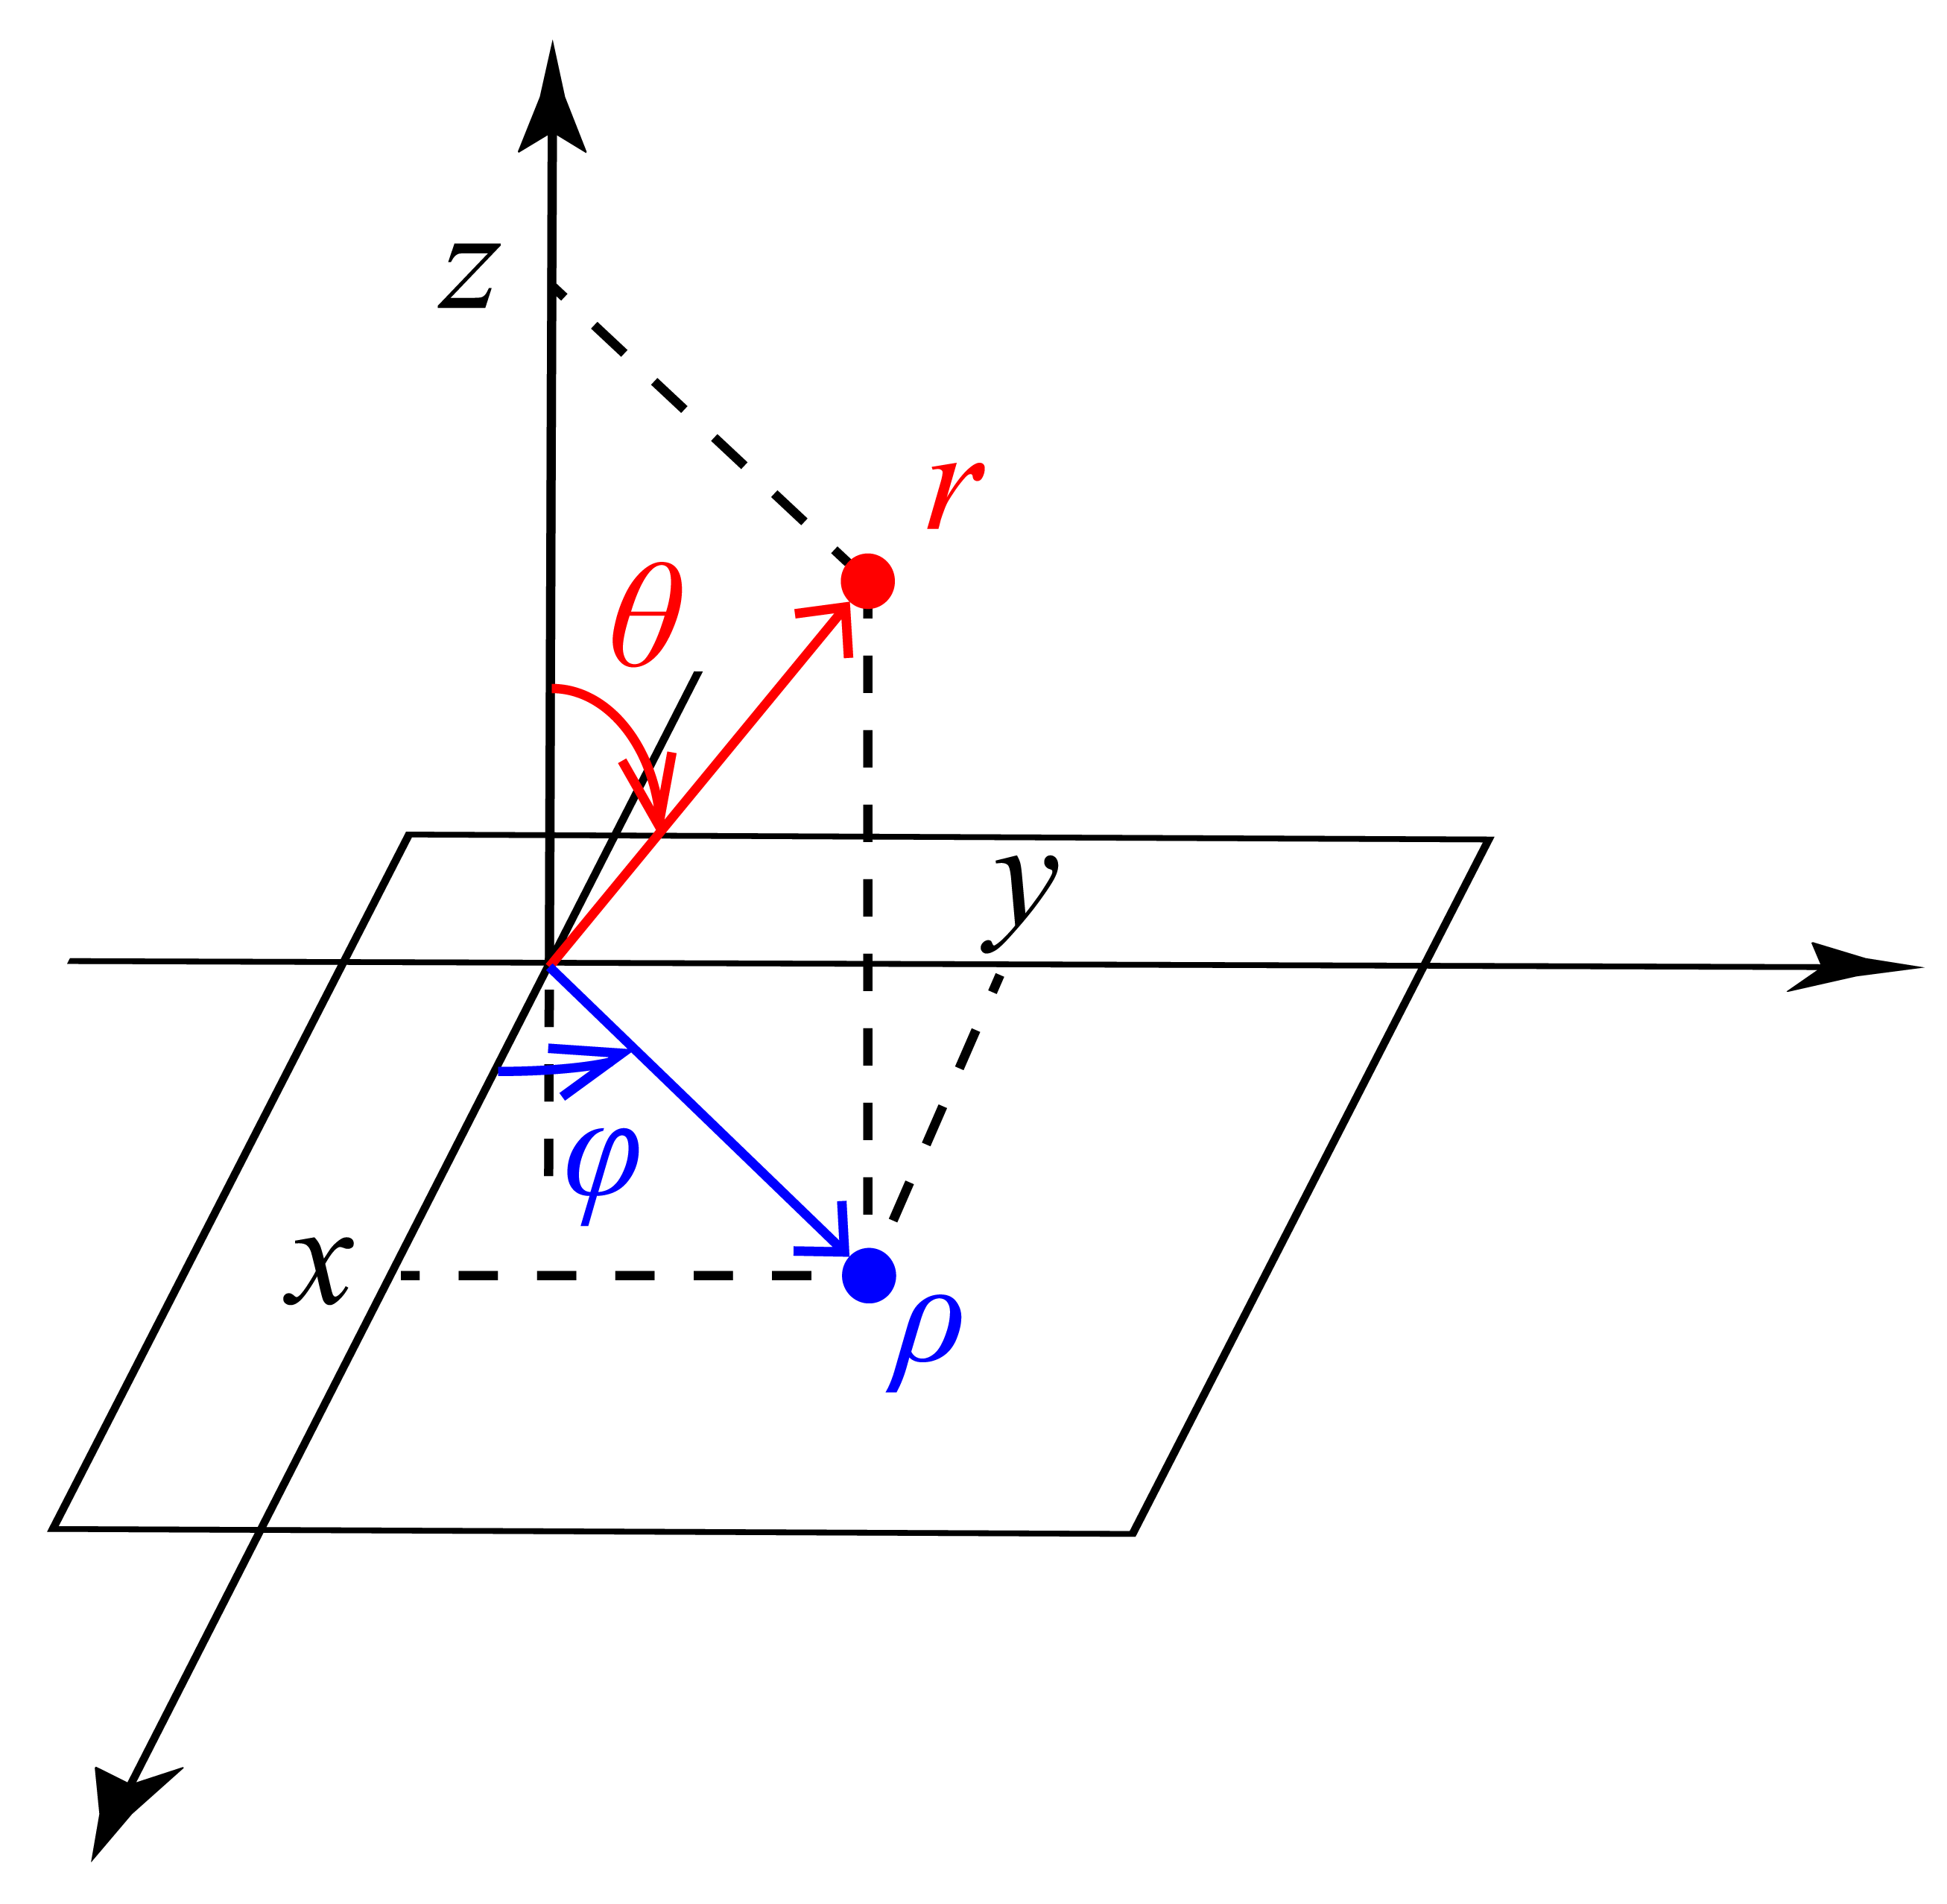
\includegraphics[width=7cm]{image/6-1-1.png}
\caption{三种坐标}
\end{wrapfigure}
需要注意,\,我们对以上$\theta,\,\varphi$角度定义比较微妙,\,$\theta$一般限制其在$[0,\pi]$范围内,\,在端点$\theta=0,\,\pi$处$\varphi$的不同取值代表同一个空间点.\,但$\varphi$的取值我们不加以任何限制,\,也就是原则上$\varphi\in\mathbb{R}$.\,而任意$\varphi$相差$2n\pi$的坐标实际上代表同一个空间点.\,这么做是因为我们最好不要用静态的几何观点去看待角度这一概念.\,而是用运动,\,变换的观点去看待角度.\,作为连续的运动的点的幅角变化也应是连续的,\,为了使点绕$z$轴一圈后幅角不至于突然改变,\,就必须默认每一点的幅角可以有多种取值,\,在具体的运动中应该灵活选择其具体取值大小.

之后经常会说到各种对称性,\,在本系列教材中我们采取如下说法:\,\emph{球对称}(spherical symmetric)仅仅代表某个函数$f(r,\theta,\varphi)$与$\varphi$无关.\,而\emph{柱对称}(cylindrical symmetric)代表的是$f(\rho,\varphi,z)$与$z$无关.\,与$\varphi$和$\theta$都无关的$f(r,\theta,\varphi)=f(r,\forall\theta,\forall\varphi)$被称为\emph{各向同性}(isotropic).\,最后\emph{中心对称}(centrosymmetric)是一个很弱的对称性,\,它仅仅代表函数在\emph{中心反演}(space inversion)下的对称性:
\[f(x,y,z)=f(-x,-y,-z)\]

绝对时空观中的时间则是一种完全与空间独立的属性.\,实际上,\,每一个空间点处的人都能感受到时间的流逝.\,十分抽象的把这些不同的时刻画在一根时间轴上,\,便是一维的时间坐标:
\[A(t)\in\mathbb{R} \quad;\quad t\in\mathbb{R}\]

而时空又是两个独立的概念.\,任意一个坐标点处都有时间轴,\,而任意一个时刻都有一个三维空间切片.\,事实上,\,我们的时空是一个3+1维的结构,\,合理地选取坐标后,\,实际上可以把时空结构写成四维坐标:
\[A(x,y,z,t)\in\mathbb{R}^4 \quad;\quad x,y,z,t\in\mathbb{R}\]

而对于任意两个时空点,\,存在绝对的时间,\,也就是可以找到两个事件的绝对时间差:
\[\tau=|t_2-t_1|\]

但空间距离却具有相对性.\,我们要求在同一时刻的同一空间切片上定义空间的度量:
\[t_1=t_2:\quad l=\sqrt{(x_1-x_2)^2+(y_1-y_2)^2+(z_1-z_2)^2}\]

不同时刻的空间,\,被线性地组织在一起,\,保证每一刻都平直的空间既不会随时间膨胀收缩,\,也不会旋转加速.\,这种时空结构被叫做\emph{牛顿-嘉当几何}(Newton-Cartan geometry)\footnote{用更为严格的语言来说,\,我们需要一个装备了一阶形式``钟''$c_\nu$和二阶逆变半正定对称张量类空间度规$s^{\mu\nu}$的四维微分流形$\mathscr{M}$:
\[\mathscr{M}:\quad s^{\mu\nu}c_{\nu}=0\]}.

时间是一个新的量纲,\,其国际单位制对$1{\rm s}$的定义为:
\begin{verse}
1s是铯-133原子基态的两个超精细能级之间跃迁所对应的辐射周期时长的9192631770倍.
\end{verse}

牛顿-嘉当几何的显著特点是物理量的定义没有所谓的\emph{协变性}(covariance).\,固然,\,在三维空间坐标框架的旋转下,\,任何物理过程中的事件所发生的位置坐标发生旋转变换,\,而几乎所有标量(比如质量,\,能量)都不变,\,几乎所有矢量(比如动量,\,角动量)都按照类似坐标变换的法则发生变换.\,但是,\,对于更普遍的一列\emph{伽利略变换}(Galilean transformation),\,也就是相对匀速运动的参考系之间的变换,\,时空坐标的形式却不能简单地推广到能量动量角动量上.

不同于绝对时空观中时间与空间成为相互独立的量纲的特点,\,狭义相对论改变了对基本物理量的看法.\,狭义相对论把时空看成为可以相互转化的不可分割的新的3+1维整体,\,同时性已然破缺.\,两个时空点之间无法定义绝对的时间间隔.\,在\emph{相对论时空观}(relativistic spacetime picture)下,\,时间和空间可以用同一把尺子去丈量:\,这是由于光速的不变性:
\[c=299792458{\rm m/s}\]

而量出来的长度叫做\emph{时空间隔}(spacetime interval):
\[\ud s^2=c^2\ud t^2-\ud x^2-\ud y^2-\ud z^2\]

这赋予时空以截然不同的结构,\,最关键的一点是,\,时间的绝对性被取消了,\,不同事件发生时间先后的比较不总是可行,\,相对论的有限速度因果律在这里取代了经典观点的时序因果律.\,我们将在 电磁学理论的最后介绍相对论理论.


\subsection{物质}

时空是物理过程发生的舞台.\,那么将物质引入后舞台上所演出的便是\emph{事件}(event).\,事件这个物理概念由这样的数学工具来描述:\,它的第一个要素自然是时空坐标$(\bs{r},t)$,\,是事件在时空上的外化.\,第二个要素是事件内禀的属性.\,它取决于所引入的物质种类,\,还取决于我们所关心问题的层次.\,一般用标量,\,矢量,\,乃至张量这样的数学工具来描述它.\,举例,\,电磁场物质在经典物理中用电场磁场来描述,\,但在\emph{量子力学}(quantum mechanics,\, QM)中这不够了,\,需要用矢势和标势来描述才是完整的.\,在更深的\emph{量子场论}(quantum field theory,\, QFT)中甚至这也是不够的.\,还需要量子化为光子才合适.\,又比如,\,电子这个很有意思的现象,\,最简单的模型是质点模型,\,内禀的属性是质量,\,动量与能量\footnote{不要认为动量能量不是内禀的而是由时空运动所决定的,\,读者可以思考在水中一个气泡的上升,\,它为体系带来的动量方向如何?}.\,然而与电磁场的经典相互作用强度告诉我们还有一项内禀属性叫做电荷量.\,近代人们惊奇地发现原来电子还固有磁矩,\,与之相应的电子具有自旋.\,最后狄拉克等人发展出\emph{量子电动力学}(quantum electrodynamics,\,QED),\,统一地用一个四分量的旋量波函数和它的方程中的若干参数来完整地描述所有发现的电子内禀属性.

\vspace{0.5cm}
\emph{经典物理学}\footnote{本书的经典物理学指牛顿力学,\,分析力学,\,经典电磁学,\,经典统计力学与狭义相对论的范畴.}(classical physics)中涉及到的物质主要有:

\vspace{0.2cm}
{\bf 1.\,质点(point mass,\,particle)}

不得不承认质点是牛顿力学的根基,\,一切可观的结论的出发点.\,质点所对应的事件集合为时空中的一条\emph{世界线}(world line).\,每一个时间仅仅有可能只有一个事件发生.\,实际上质点的运动用\emph{运动学方程}(kinematic equation)来描述:
\[\bs{r}=\bs{r}(t)=\left(x(t),y(t),z(t)\right)\]

而\emph{质量}(mass)是质点必要的内禀属性.\,它将作为参数出现在下一节介绍的动力学方程中.\,它反应物质受到同样大小的相互作用运动状态改变的难易程度.\,国际单位制从1889年至2018年末对$1\rm kg$的定义如下:

\begin{verse}
1kg是保存在法国巴黎布勒特伊宫的国际计量局实验室的约47立方厘米立式铂铱合金小圆柱的质量.\,当然,\,出于实用考虑,\,也是很多它的官方复制体的质量.
\end{verse}

这个定义今已经有一百多年了,\,历史远长于其他六个国际基本单位.\,但目前这一古老的定义方式已经被废除,\,新的定义\footnote{一方面,\,它依赖于狭义相对论和量子力学的正确性,\,目前极少理论物理工作者会质疑它.\,另一方面,\,应该要先定义上文的1s和1m,\,再来定义1kg.}为:

\begin{verse}
1kg被这样定义:\,取普朗克常数的固定数值在单位$\rm kg\cdot m^2\cdot s^{-1}$下为$\rm 6.62607015\times 10^{-34}$.
\end{verse}

长度,\,时间和质量为三大力学量纲,\,量纲是物理量的属性,\,物理量的表示方法为数值加单位,\,每个量纲有自己独特的一套单位,\,不同单位间差一个纯数的倍率.\,在物理量的加减时量纲必须相同而且结果保持量纲不变.\,但不同量纲物理量可以进行乘除而生成新的量纲.\,除了简单的加减乘除的以上规则以外,\,其他特殊函数必须只能作用在无量纲的纯数上.\,这叫做\emph{量纲法则}(dimensional rules).

\vspace{0.2cm}
{\bf 2.\,质点系(particle system)}

质点系是对质点的一种自然扩展.\,讨论质点的运动时质点受到的相互作用来自何方?\,在牛顿力学的框架下必然来自施力物体.\,故把受力物体和施力物体都作为简单的质点时,\,两个质点就可以作为整个体系讨论,\,把相互作用区分为内力与外力而推广之前的结论,\,在这个过程中我们能体会到哪些结论是一脉相承的普遍规律而哪些需要重新审视与修改.\,从原理上质点系不过是多个质点同时存在的情况而已.\,而\emph{经典统计力学}(classical statistic mechanics)是这种观点的提炼与延伸,\,它着眼于一个宏观大分子数的体系的长时间平均下的行为,\,理论上常常结合概率论的做法,\,对等概率的体系代表点构成的系综做平均.\,从中提取统计力学下不平凡的物理量.

\vspace{0.2cm}
{\bf 3.\,连续介质(continuous media)}

一方面,\,连续介质是从纯粹的理论过渡到实际问题的至关重要一步.\,另一方面,\,在处理连续介质的问题中形成了场论,\,它作为了一种与质点截然不同的物理图像形成了自己的一整套理论.\,更重要的,\,量子场论认为由于不确定原理,\,质点与世界线的观点实际上是作为场的传播的一种近似.\,也就是说,\,场论相比质点的力学更具有兼容性和普适性.\,对于简单的连续介质,\,内禀的属性由每一个点处的质量密度$\rho$和速度$\bs{v}$描述,\,这实际上形成了一个标量场和矢量场:
\[\rho=\rho(\bs{r},t) \quad;\quad \bs{v}=\bs{v}(\bs{r},t)\]

而动力学方程的列法又强烈依赖于介质内的相互作用.\,于是这个大的问题又分出很有代表性的弹性力学和流体力学,\,还有介于两者之间的粘弹性塑性模型等等.\,还有从热力学平衡态出发考虑的近平衡态统计力学方法.

\vspace{0.2cm}
{\bf 4.\,场(field)}

\begin{wrapfigure}[16]{o}[-10pt]{7cm}
\vspace{-0.4cm}
\centering
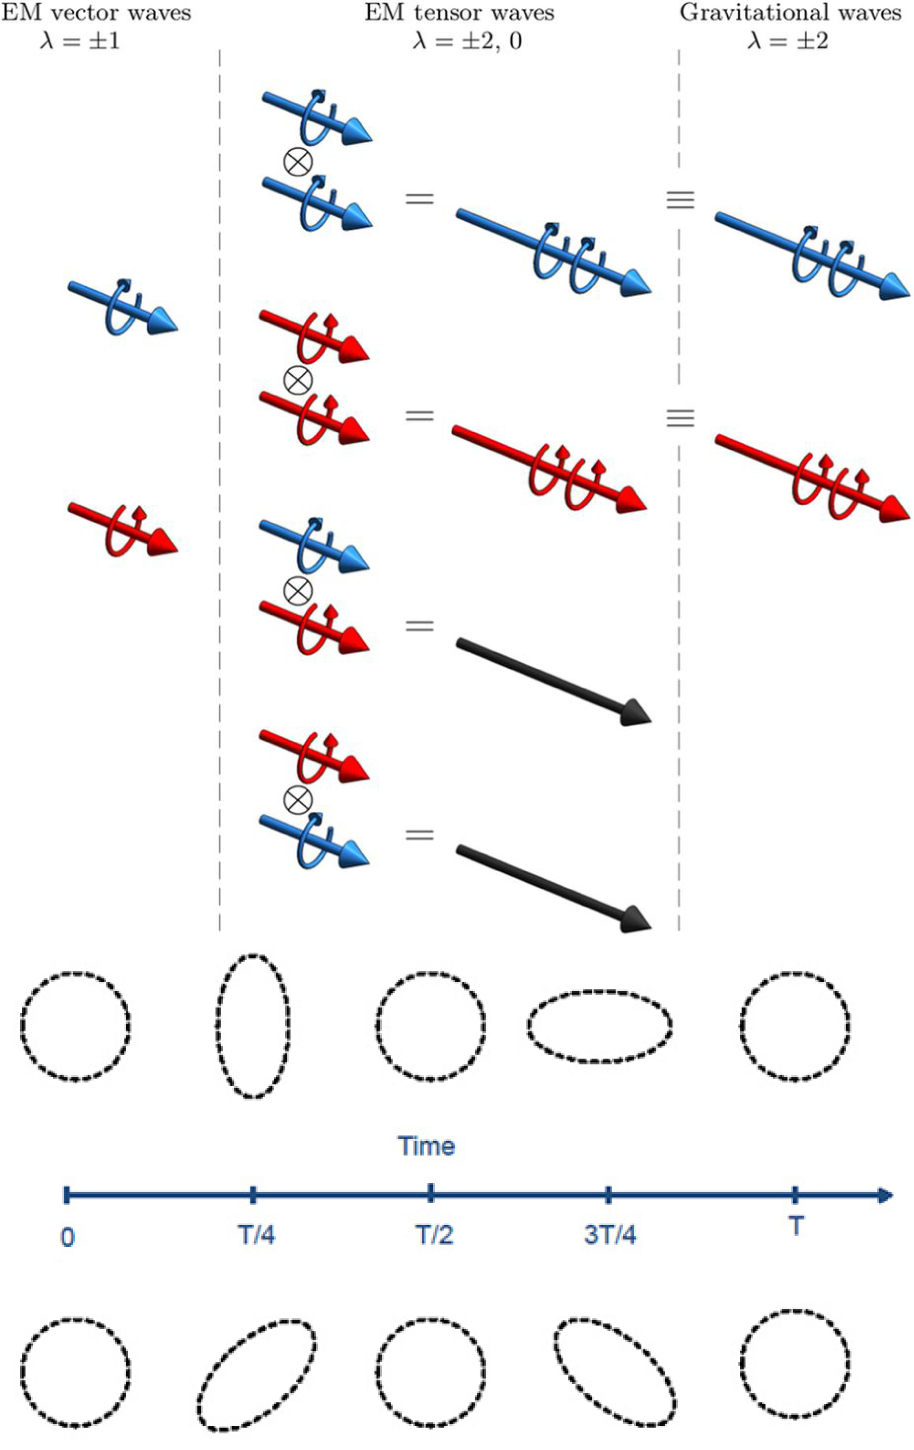
\includegraphics[width=5cm]{image/6-1-2.png}
\caption{引力波与电磁波的区别}
\end{wrapfigure}
关于场的理解历史上经历了两个过程.\,第一个阶段是正如上面的连续介质的做法,\,场是作为某种事先已经被研究的足够清楚的粒子体系与它们之间的相互作用的描述方法与数学工具.\,而从牛顿时代开始人们就默认了超距作用的存在,\,而场数学工具的第二个作用就是描述电荷之间,\,质量之间的超距作用.\,但是逐渐人们意识到相互作用传播速度的有限性,\,于是场开始变成某种与物质其他耦合的物质而单独存在,\,这就是第二阶段,\,人们意识到了场本身就是一种物质,\,电子与电子之间不能直接相互作用,\,电子改变了真空,\,稳定地与电磁场相互作用而产生库仑场,\,然后在对第二个电子产生相互作用力.\,将场作为某种先验地存在于时空中的物质形式进行描述与研究的学科就叫做\emph{场论}(field theory).\,有哪些可能的场形式?\,场的物理量如何书写?\,场与粒子,\,场与场之间如何相互作用便是场论的研究内容.\,比如说,\,动力学所关心的内容,\,场的质量本身没有定义,\,可以定义的一般是场的定域动量与波矢,\,能量与角频率,\,平面波的色散关系等等.\,的确,\,场论最基本的做法是傅里叶分解,\,它认为平面波是不受任何相互作用时的场的惯性运动方式,\,而任何场的运动,\,每一时刻都可以分解成一系列平面波的叠加.\,就好像任何复杂体系的运动本质上都是质点系的运动,\,而质点的运动每时每刻都可以看出匀速运动那样.


场论根据其描述方法分为标量场论,\,矢量场论,\,张量场论和旋量场论等.\,电磁场论是矢量场论,\,它用四势矢量$(\varphi,\bs{A})$来描述.\,引力场论在广义相对论弱场近似下是张量场论,\,但传播的引力波和电磁波类似只能有两种偏振,\,其模式为$+$型和$\times$型,\,这又是不同于电磁波的.\,在更现代的观点中,\,场是真空的某种激发,\,十分类似于一张二维的拉紧的薄膜,\,没有任何振动时它已经固有能量了,\,场物质反应为膜的各种振动形式.\,而一个石子受到外力而压弯了膜,\,就可以理解为粒子与场之间的相互作用.



\subsection{参考系,\,物理规律与其不变性}

\emph{坐标系}(coordinate system)是一套用来描述时空点位置的坐标系统,\,而\emph{参考系}(reference system)则是下文将引申的一类坐标系的统称.

在伽利略时空观\footnote{本章仅限讨论非相对论,\,相对论见后}下参考系的定义相对简单.\,我们只需要任意指定一个观察者,\,观察者可以在$3+1$维的时空中作任意运动,\,每一个时刻对应一个测量的坐标系统:\,观察者分别以右手边,\,胸前和头顶三个方向建立坐标系,\,坐标系的刻度就是其代表的位置到原点观察者处的空间距离.\,这样便可以表示任意事件的时空坐标.\,而且构成一个三维空间直角坐标系.\,叫做观察者的\emph{固有参考系}(proper reference system).

物理规律的本质是什么?\,在一个特定的参考系中,\,我们进行一些物理量的测量,\,测量得到的值之间在特定的实验条件下会满足特定的关系而不依赖于某些具体的参数,\,一般都是等式.\,这样的普遍成立的等式就可以反映某些物理规律.\,从\emph{动理学}(kinetics)的角度理解,\,体系的演化是\emph{状态}(state)随时间的演化,\,而体系的状态由一组完备的\emph{态参量}(state variable)描述,\,态参量可以包含一些广义坐标$q_\alpha$和他们对时间的导数即广义速度$v_\alpha=\dot{q}_\alpha$.\,而以下\emph{决定论}(determinism)则对物理规律的形式做出了规定:
\begin{quote}
动理学系统:

已知某时刻$t=0$的初态$\{q_\alpha(0),\,\dot{q}_\alpha(0)\}$后,\,应能预言任意将来的状态$\{q_\alpha(t),\,\dot{q}_\alpha(t)\}$.
\end{quote}

事实上,\,不光是将来的状态,\,在一般经典物理的框架下,\,过去的状态也是可以被``预言''的.\,这是因为我们进一步要求动理学系统的规律是以下形式的二阶方程:
\[f_i(\ddot{q}_\alpha,\,\dot{q}_\alpha,\,{q}_\alpha,\,t)=0\]

而且广义坐标的个数应该和方程的数目一致,\,方程是至多二阶的.\,微分方程的描述在数学上完全导致了体系彻底的决定性,\,只要知道初始条件便可以往前往后推理所有发生的物理现象\footnote{更有甚者,\,经典物理也难以解释耗散现象,\,在忽略耗散时,\,方程应该还具有平移对称性(不显含t)和时间反演对称性(方程对广义速度是偶函数).\,此时对将来和对过去的预言在广义速度取相反数时是完全对称的,\,而且预言只依赖于时间差不依赖于初始时刻.}.

这一物理学科研究范围内的有关决定性的原理很强大,\,强大到历史上很多物理学家和哲学家都质疑过它的真实性和适用性.\,最著名的莫过于拉普拉斯提出的\emph{拉普拉斯妖}(Laplace's demon)的论点:\,如果存在一个全知的拉普拉斯妖,\,能够知道在某一时刻宇宙中所有原子的精确位置与动量,\,那么任意时刻的状态也能被预言.\,这种决定论观点总是被拿来与\emph{自由意志论}(free will)去归谬,\,如果过去与未来都已经被谱写,\,那么人类所有的行为的意义和动机也就不能被解释.\,这直到今天也是科学与哲学未能获得满意的回答的问题.

但是科学的一个目的就是在于能够对未发生的事情进行预言,\,所以本着对决定论的认可与尊重,\,我们才能继续我们的科学研究.

\vspace{1cm}

除了需要符合决定性原理,\,物理规律还需要反映出一定的对称性.\,整个牛顿的\emph{经典力学}(classical mechanics)体系都要遵从的一个大的对称性,\,我们可以称之为\emph{伽利略对称性}(Galilean symmetry),\,也是伽利略时空观的一个重要组成部分.\,这个对称性的含义如下阐释:

首先我们重拾``绝对时空观''的说法.\,其含义是存在一个特殊的观察者,\,它建立的坐标系$O-xyz$(对位于原点的观察者来说,\,是参考系)是默认的第一个使得我们以上提出的物理规律成立的坐标系.\,自身具有$3+1$维的结构:
\[(x,\,y,\,z,\,t)\in \mathbb{R}^3\times \mathbb{R}\quad,\quad \ud l^2=\ud x^2+\ud y^2+\ud z^2\]

\begin{figure}[H]
\centering
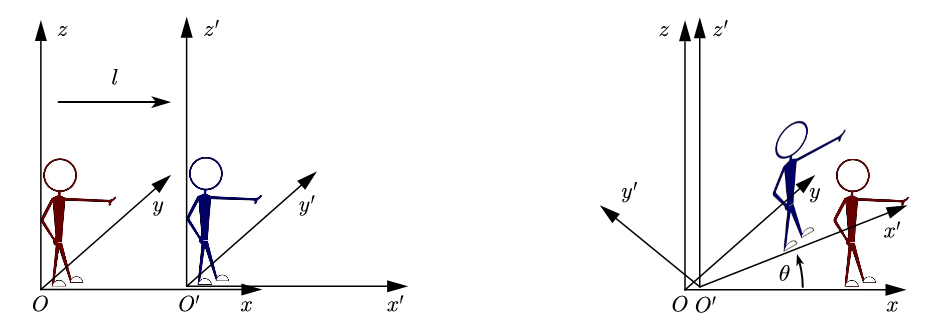
\includegraphics[width=12cm]{image/6-1-15.png}
\caption{固定平移与转动}
\end{figure}

让我们来阐明参考系与坐标系之间的区别.\,我们设想另外一个观察者,\,它与原观察者保持相对静止.\,但是其建立的坐标系$O'-x'y'z'$依然可能有很多种可能性:\,默认观察者自己为原点,\,右手边为$x$轴,\,胸前为$y$轴,\,头顶为$z$轴.\,一种可能性是,\,新观察者相对原来的观察者仅仅是做时空\emph{平移}(translation),\,而其轴的方向保持平行.\,






\section{运动的描述}

\subsection{质点的运动}
质点的运动是复杂的连续体的运动的基础.\,所谓\emph{运动}(motion)就是每一个时间都有一个位置.\,就是说位置是时间的函数:
\[\bs{r}=\bs{r}(t)\]

我们使用实数上的矢量空间和矢量来刻画真实的物理学上的二维或三维空间和其中的点.\,也即:
\[\bs{r}\in\mathbb{R}^2 \;{\rm or}\; \mathbb{R}^3\]

\begin{wrapfigure}[16]{o}[-10pt]{7cm}\label{6-1-3}
\vspace{-0.4cm}
\centering
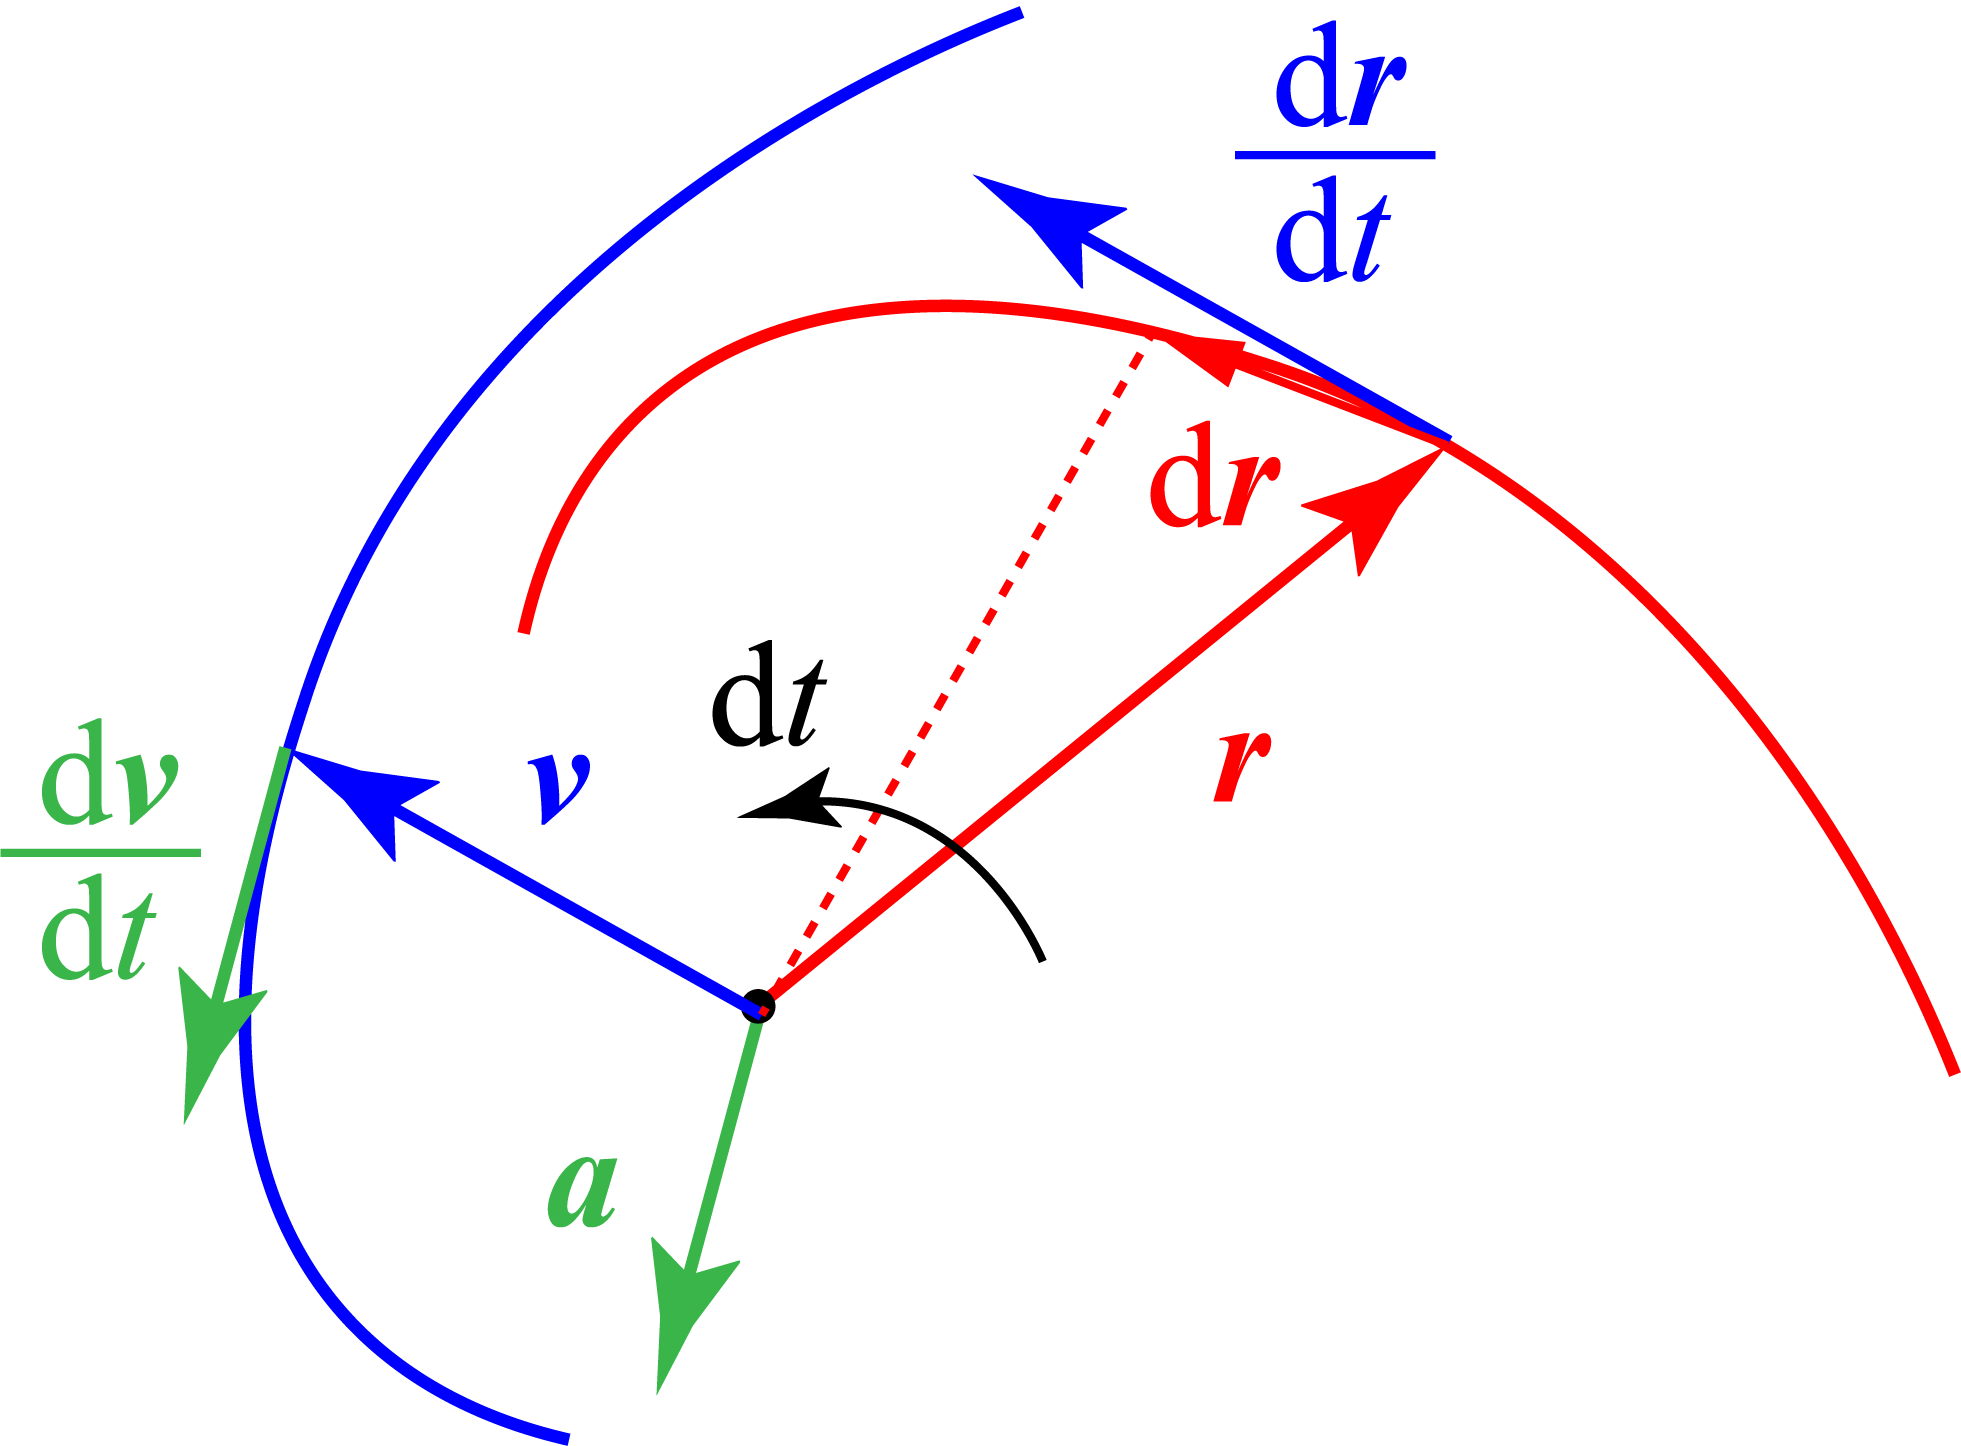
\includegraphics[width=7cm]{image/6-1-3.png}
\caption{质点的位置,\,速度与加速度}
\end{wrapfigure}
前者对应二维运动,\,后者对应三维运动.\,我们从中可以发现,\,函数是描述运动的数学工具,\,对矢量与函数的分析学知识便是运动学和物理学的基础.\,而运动学本身是可以看成是数学的一个分支的.\,对质点的位置矢量求导数便得到速度矢量,\,再求导数或是求二阶导数便是加速度矢量:
\[\bs{v}=\frac{\ud \bs{r}}{\ud t}=\lim_{\Delta t\to 0 }\frac{\bs{r}(t+\Delta t)-\bs{r}(t)}{\Delta t}\]
\[\bs{a}=\frac{\ud \bs{v}}{\ud t}=\lim_{\Delta t\to 0 }\frac{\bs{v}(t+\Delta t)-\bs{v}(t)}{\Delta t}\]
\[\bs{a}=\frac{\ud ^2\bs{r}}{\ud t^2}=\lim_{\Delta t\to 0 }\frac{[\bs{r}(t+\Delta t)-\bs{r}(t)]-[\bs{r}(t)-\bs{r}(t-\Delta t)]}{\Delta t^2}\]

正如上图\ref{6-1-3}所示,\,我们可以把每一个瞬时的速度矢量共起点画出来,\,并把端点连做曲线,\,此时背景的空间往往叫做\emph{速度空间}(velocity space),\,它的更普遍的对应是动量空间,\,这在近代物理的理论值具有重要地位.\,引入速度空间后质点的运动便可以等价地在速度空间中进行研究.\,比如在均匀重力场中的抛体运动在速度空间中就是简单的竖直向下的匀速直线运动.\,而平方反比力下的天体运动(开普勒问题)实际上在速度空间中可以证明将变为变速偏心圆周运动.\,这使得通过速度求加速度就好像通过位置求速度那样方便.\,具体求法接下来还得进一步展开.

加速度的导数偶尔也会进入物理研究的视野,\,它被叫做\emph{急动度}(jerk).\,即:
\[\bs{j}=\frac{\ud \bs{a}}{\ud t}=\frac{\ud ^3\bs{r}}{\ud t^3}\]

矢量函数概念就是实数到矢量的映射,\,但是具体能写出函数形式的例子在物理中却不是那么常见.\,比如抛体运动的运动对应的函数,\,即\emph{运动方程}(equation of motion)\footnote{指运动学运动方程,\,动力学运动方程就是反应运动的规律的,\,能够最终解出来运动学运动方程的微分方程.}为:
\[\bs{r}=\bs{r}_0+\bs{v}_0 t+\frac{1}{2}\bs{g}t^2\]

它是牛顿定律下以下微分方程结论的解:
\[\bs{a}=\frac{\ud ^2\bs{r}}{\ud t^2}=\bs{g}\]

但是在一般情况下,\,要表示出一个既有大小又有方向的矢量函数,\,我们得采用分解的思想,\,研究能够完全确定这个矢量值的参数.\,通常有以下做法:

\vspace{0.2cm}
{\bf 1.\,直角坐标系下的分解}

在一个欧几里得空间里的一个参考系中研究问题,\,很常见的一种做法是建立直角坐标系来表示一个点的位置.\,以更普遍的三维运动为例.\,既然物体的位置由坐标$(x,\,y,\,z)$来表示.\,我们就能认为表示运动的任务由三个标量函数$x(t),\,y(t),\,z(t)$来承担.\,其实这与上面介绍的用矢量来表示位置是非常一致的,\,因为实际上点的坐标通常也被理解为原点指向这个点的矢量在三个基矢的坐标:
\[\bs{r}=(x,\,y,\,z)=x\bs{i}+y\bs{j}+z\bs{k}\]

出于哈密顿(Hamilton)爵士关于把三维空间三个方向基矢视作四元数代数运算的旋转等效的奇妙观点,\,我们分别把$x,\,y,\,z$方向的基矢按照惯例记做$\bs{i},\,\bs{j},\,\bs{k}$.\,也常常因为它们是单位矢量(长度为1),\,而记做$\bs{e}_x,\,\bs{e}_y,\,\bs{e}_z$.\,这样便能把$\bs{r}$分解出$x$,\,$y$,\,$z$来.

分解以后,\,重新合成便能得到需要的物理量.\,这其中的意思是:\,比如我们为了求一个曲线运动速度或者加速度的$x$分量.\,也就是求下列表达式:
\[\bs{v}=v_x\bs{i}+v_y\bs{j}+v_x\bs{k}=\frac{\ud \bs{r}}{\ud t}\]
\[\bs{a}=a_x\bs{i}+a_y\bs{j}+a_x\bs{k}=\frac{\ud^2 \bs{r}}{\ud t^2}\]

中的分量$v_x,\,a_x$.\,其求法非常直接,\,便是:
\[v_x=\frac{\ud }{\ud t}x(t)\quad,\quad a_x=\frac{\ud^2 }{\ud t^2}x(t)\]

这相当于是说,\,求导数和向某固定方向投影是可以交换前后次序的:

\[\bs{i}\cdot \frac{\ud }{\ud t}\bs{r}=\frac{\ud }{\ud t}(\bs{i}\cdot \bs{r})\quad,\quad \bs{i}\cdot \frac{\ud }{\ud t}\bs{v}=\frac{\ud }{\ud t}(\bs{i}\cdot \bs{v})\]

这是当然的,\,因为矢量点乘的导数的法则也符合与标量乘积求导数类似的莱布尼茨法则,\,而常矢量$\bs{i}$不随着运动改变.\,所以导数只有对$\bs{r},\,\bs{v}$求导的项.

在数学上,\,曲线段也经常被描述为是与某实数上区间\emph{同胚}(homeomorphic)的几何图形,\,这其实就是说,\,存在自变量$t$,\,不失一般性地,\,我们让其取值范围为$(-\infty,\,+\infty)$.\,而存在一个从这个自变量到三维空间点$(x,\,y,\,z)$的光滑映射:
\[x=x(t)\quad ,\quad y=y(t)\quad ,\quad z=z(t)\]

\begin{wrapfigure}[10]{o}[-10pt]{7cm}\label{6-1-4}
\vspace{-0.4cm}
\centering
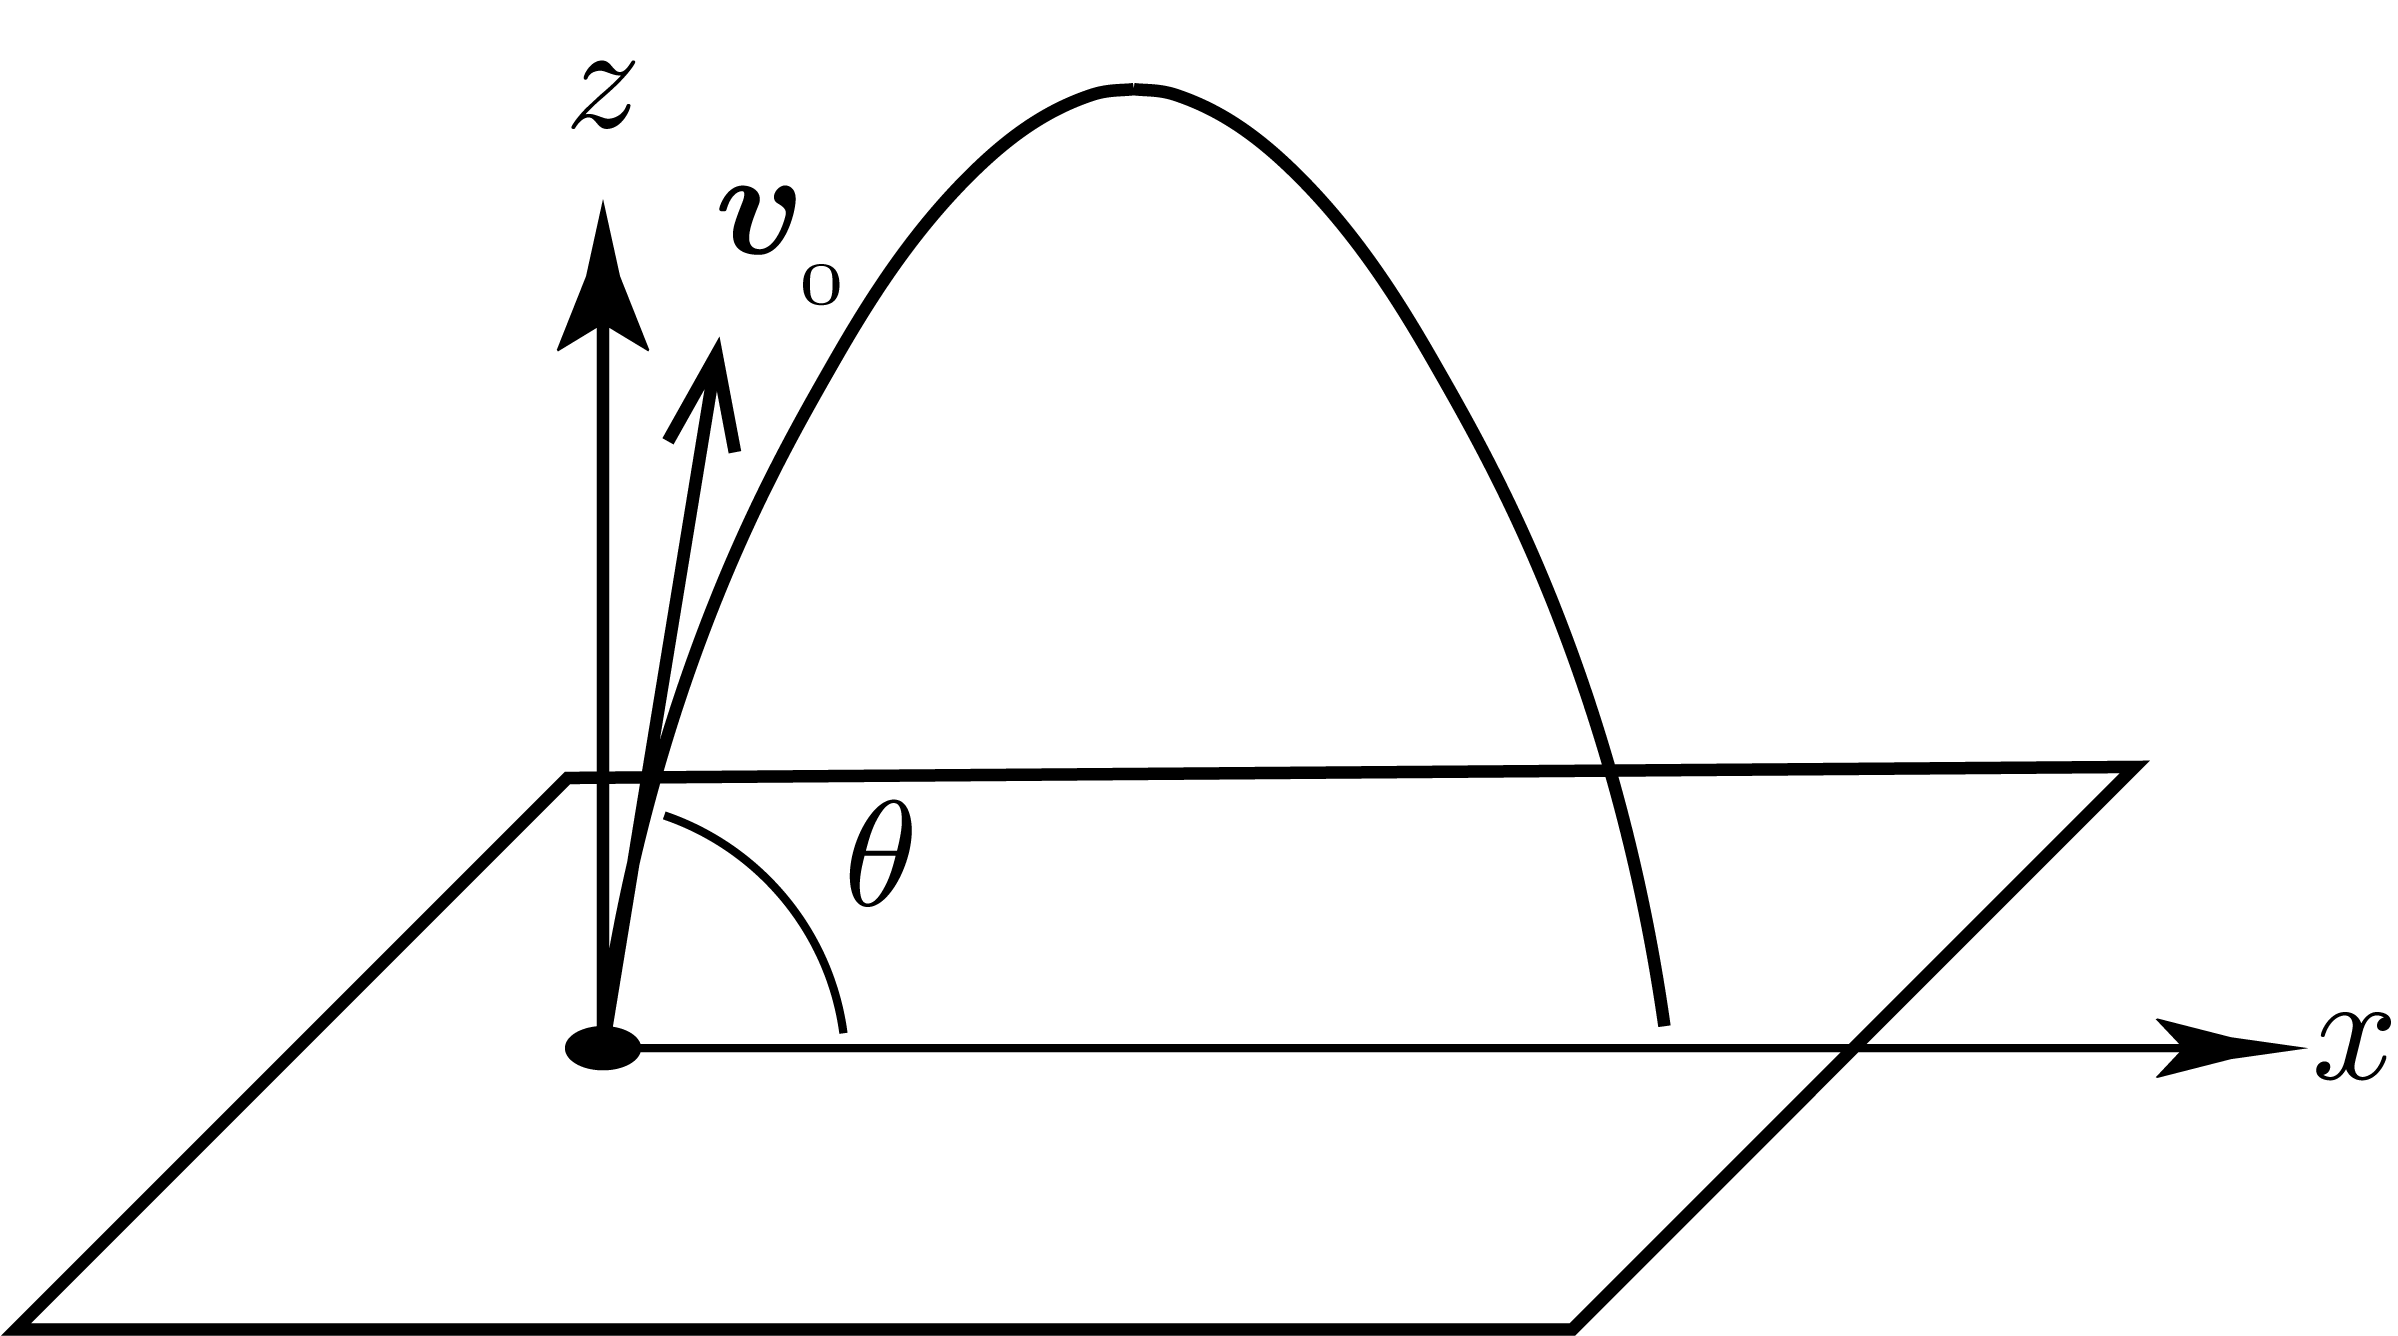
\includegraphics[width=7cm]{image/6-1-4.png}
\caption{抛体运动}
\end{wrapfigure}
在数学上看,\,这其实就是曲线方程:\,其参数方程的唯一给法.\,这样的式子就给出了几何学上的光滑曲线的定义.\,而不同于以往我们对曲线是$y=f(x)$的图像的刻板认识.\,但在这里,\,我们恰巧发现如果把参数$t$理解为时间的话,\,这恰好就对应到了一个粒子在三维空间中的运动,\,出于这样的原因,\,我们把反应了粒子位置随着时间变化的方程称为运动方程.\,它是\emph{轨迹方程}(function of trajactory)的一种特殊情况.\,对于轨迹方程,\,我们只需要通过符合方程的点$(x,\,y,\,z)$构成粒子所有运动中经过的位置构成的集合即可.\,例如,\,在地面$z=0$出发以仰角$\varphi$斜抛一个物体.\,那就以出发点为原点建立坐标系,\,竖直向上为$z$轴,\,抛的方向向前为$x$轴.\,那么运动方程为:
\[\left\{\begin{array}{l} x=v_0 t\cos\varphi\\ z=v_0 t\sin\varphi - \dfrac{1}{2}gt^2\end{array}\right.\]

但是轨迹方程不仅可以写成以上形式,\,还可以消去$t$得到:
\[z=x\tan\varphi -\frac{gx^2}{2v_0^2}(1+\tan^2\varphi)\]

\vspace{0.2cm}
{\bf 2.\,平面极坐标系下的分解}

如果质点做平面运动,\,那么我们问题得到了简化.\,此时往往有些情形下我们关心从原点的观察者出发看质点的运动时,\,质点离观察者的距离和质点相对观察者的方位.\,故引入\emph{极坐标系}(polar coordinate system)是自然而然的做法.\,其步骤为:\,确定观察者位置为\emph{极点}(pole),\,引出一条原点出发的射线为\emph{极轴}(polar axis);\,测量质点位置到极点距离$r$为\emph{矢径}(radius);\,从极点指向质点位置形成矢量矢径$\bs{r}$,\,测量极轴绕极点沿指定的正方向旋转到与矢径重合时旋转的角度$\theta$为\emph{极角}(polar angle).\,描述质点的位置时,\,$(r,\,\theta)$即构成极坐标.

仍然,\,极坐标可以用来表示质点的唯一位置:\,只需要给出$(r,\,\theta)$就可以确定位置.\,所以只要知道函数$r(t),\,\theta(t)$就能够确定其运动,\,这便是极坐标下的运动方程.\,同理如果消去$t$就能得到另一类轨迹方程.\,只要物体运动轨迹不经过极点,\,我们总是取$r(t),\,\theta(t)$为光滑的函数.\,$\theta$的取值为$(-\infty,\,+\infty)$以保证运动的连续性.\,不过$\theta$相差$2k\pi,\,k\in\mathbb{Z}$的所有坐标表示运动过程中的同一位置.

例如,\,在之前的抛体运动中,\,如果取$z$轴为极轴,\,那么其极坐标下的运动方程为:
\[\left\{\begin{array}{l} r^2=(\bs{v}_0 t+\dfrac{1}{2}\bs{g}t^2)^2=\dfrac{1}{4}g^2t^4  -gv_0t^3\sin\varphi + v_0^2t^2\\[3pt] \tan\theta=\dfrac{2v_0 \cos\varphi}{2v_0 \sin\varphi-gt}\end{array}\right.\]

这会有利于我们分析一些问题.\,例如如果关心以何种倾角抛出一个物体,\,物体离我们的距离会越来越远?\,就只需要让$r$为关于$t$的增函数,\,除了对$r$求导的做法,\,一种更加明智的做法可能是注意到关系式:
\[\frac{\ud r}{\ud t}>0  \quad\Leftrightarrow\quad	\frac{\ud}{\ud t}(\frac{1}{2}r^2)>0\]
\begin{align*} 
\Leftrightarrow \frac{\ud}{\ud t}(\frac{1}{2}r^2)	&=\frac{\ud}{\ud t}(\frac{1}{2}{\bs{r}\cdot\bs{r}})=\bs{r}\cdot\bs{v}\\
																			&=(\bs{v}_0 t+\dfrac{1}{2}\bs{g}t^2)\cdot(\bs{v}_0 +\bs{g}t)>0\\
\end{align*}

\[\Leftrightarrow (\bs{v}_0 +\dfrac{1}{2}\bs{g}t)\cdot(\bs{v}_0 +\bs{g}t)=\dfrac{1}{2}g^2t^2  -\dfrac{3}{2}gv_0t\sin\varphi + v_0^2>0\]

这就化为求关于$t$的二次函数恒大于零的系数条件问题,\,结论是初等的:\,判别式小于零:
\[\left(\dfrac{3}{2}gv_0\sin\varphi\right)^2-4\left(\dfrac{1}{2}g^2 \right)(v_0^2)<0\quad \Rightarrow\quad \sin\varphi<\frac{2\sqrt{2}}{3}\]

\begin{wrapfigure}[12]{o}[-10pt]{6cm}\label{6-1-5}
\vspace{-0.4cm}
\centering
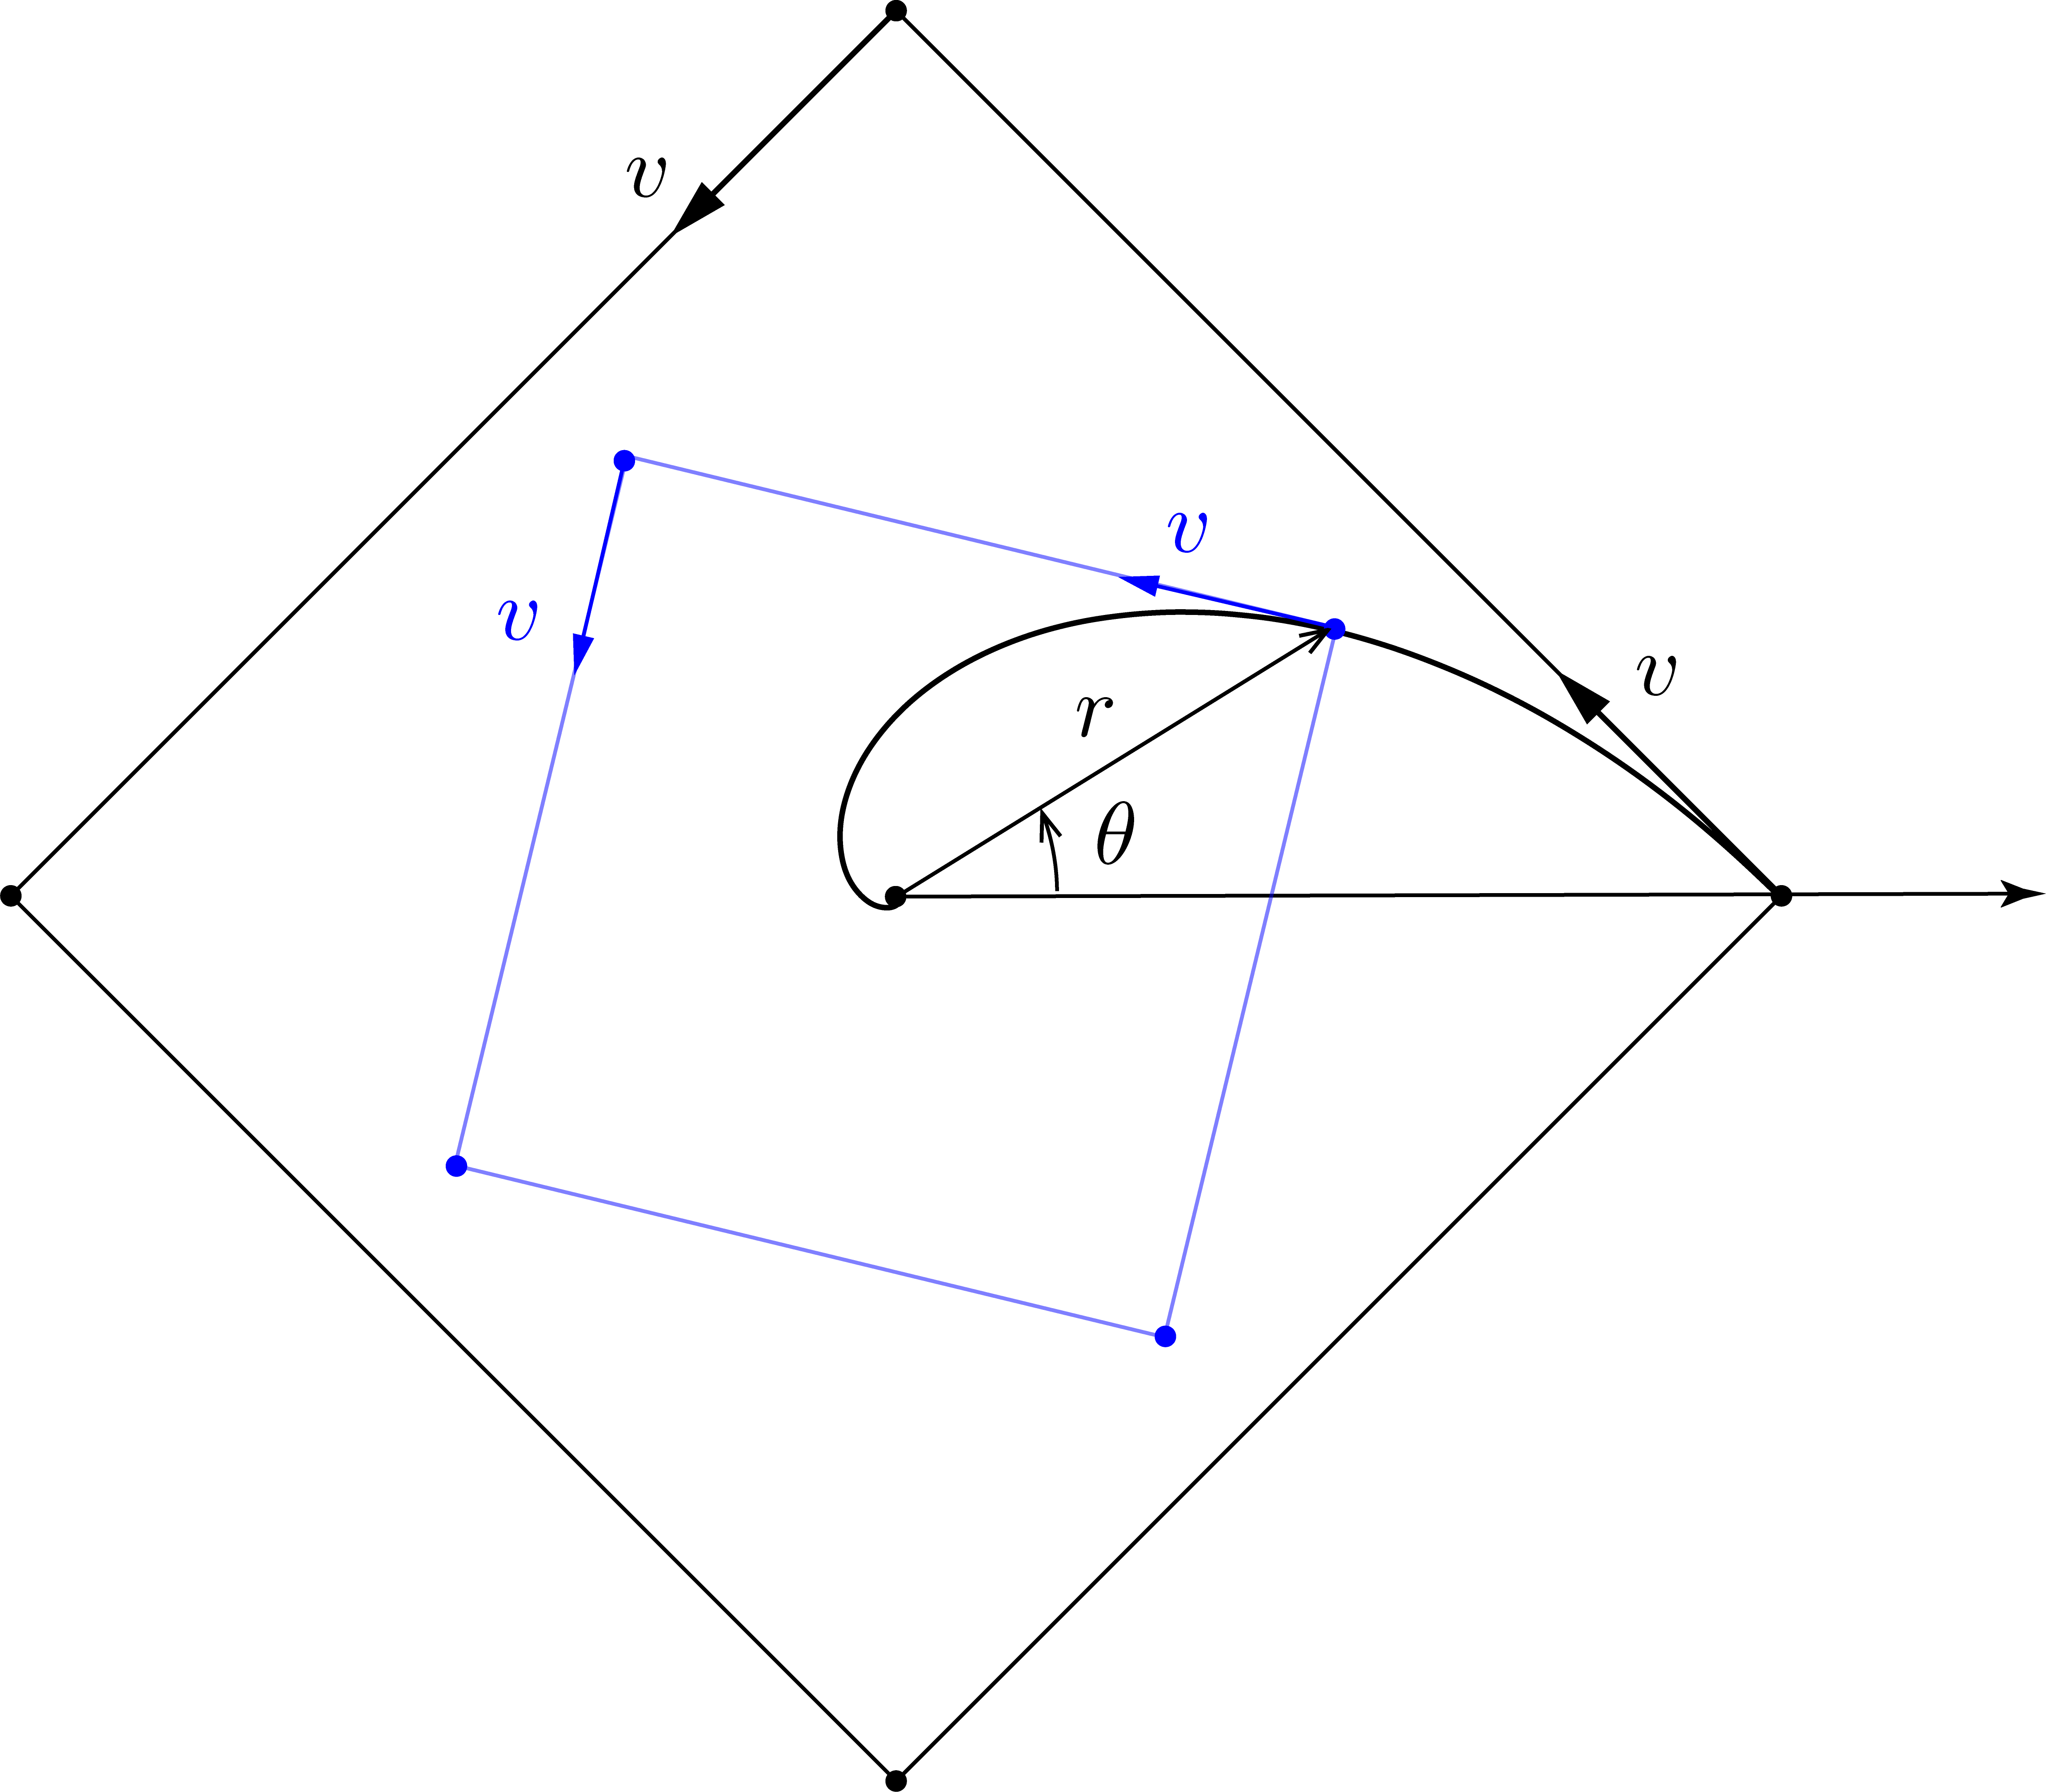
\includegraphics[width=6cm]{image/6-1-5.png}
\caption{首尾相追}
\end{wrapfigure}
采用极坐标系描述抛体运动也许是费力而不讨好的.\,但是描述其他一些运动又比直角坐标系存在天然的优势.\,比如一类经典追击问题的表述如下:\,四个平面运动的质点初始组成正方形.\,这个环形的结构中每一个质点都向着前一个质点运动发生追击.\,其中运动速度矢量具有变化的方向,\,即向着前方质点.\,但具有不变的速率$v$.\,确定物体的运动方程和轨迹.

对于这个问题,\,预先的关于物体在时间为$t$时的位置信息是几乎完全空缺的,\,但对于速度矢量我们知道一个信息:\,其大小为$v$.\,如果考虑直角坐标系,\,这个条件表示为:
\[|\bs{v}|=\sqrt{\dot{x}^2+\dot{y}^2}=v\]

但是对于位置和速度,\,我们还知道一个信息,\,就是它们夹钝角而且为$3\pi/4$.\,用直角坐标系的公式仔细化简的话也可以得到:
\[\tan \phi_{\bs{r}\curvearrowright \bs{v}}=-1\quad \Rightarrow \quad \frac{\bs{r}\cdot\bs{v}}{|\bs{r}\times \bs{v}|}=\frac{x\dot{x}+y\dot{y}}{x\dot{y}-y\dot{x}}=-1\]

\begin{wrapfigure}[12]{o}[-10pt]{6cm}\label{6-1-6}
\vspace{-0.4cm}
\centering
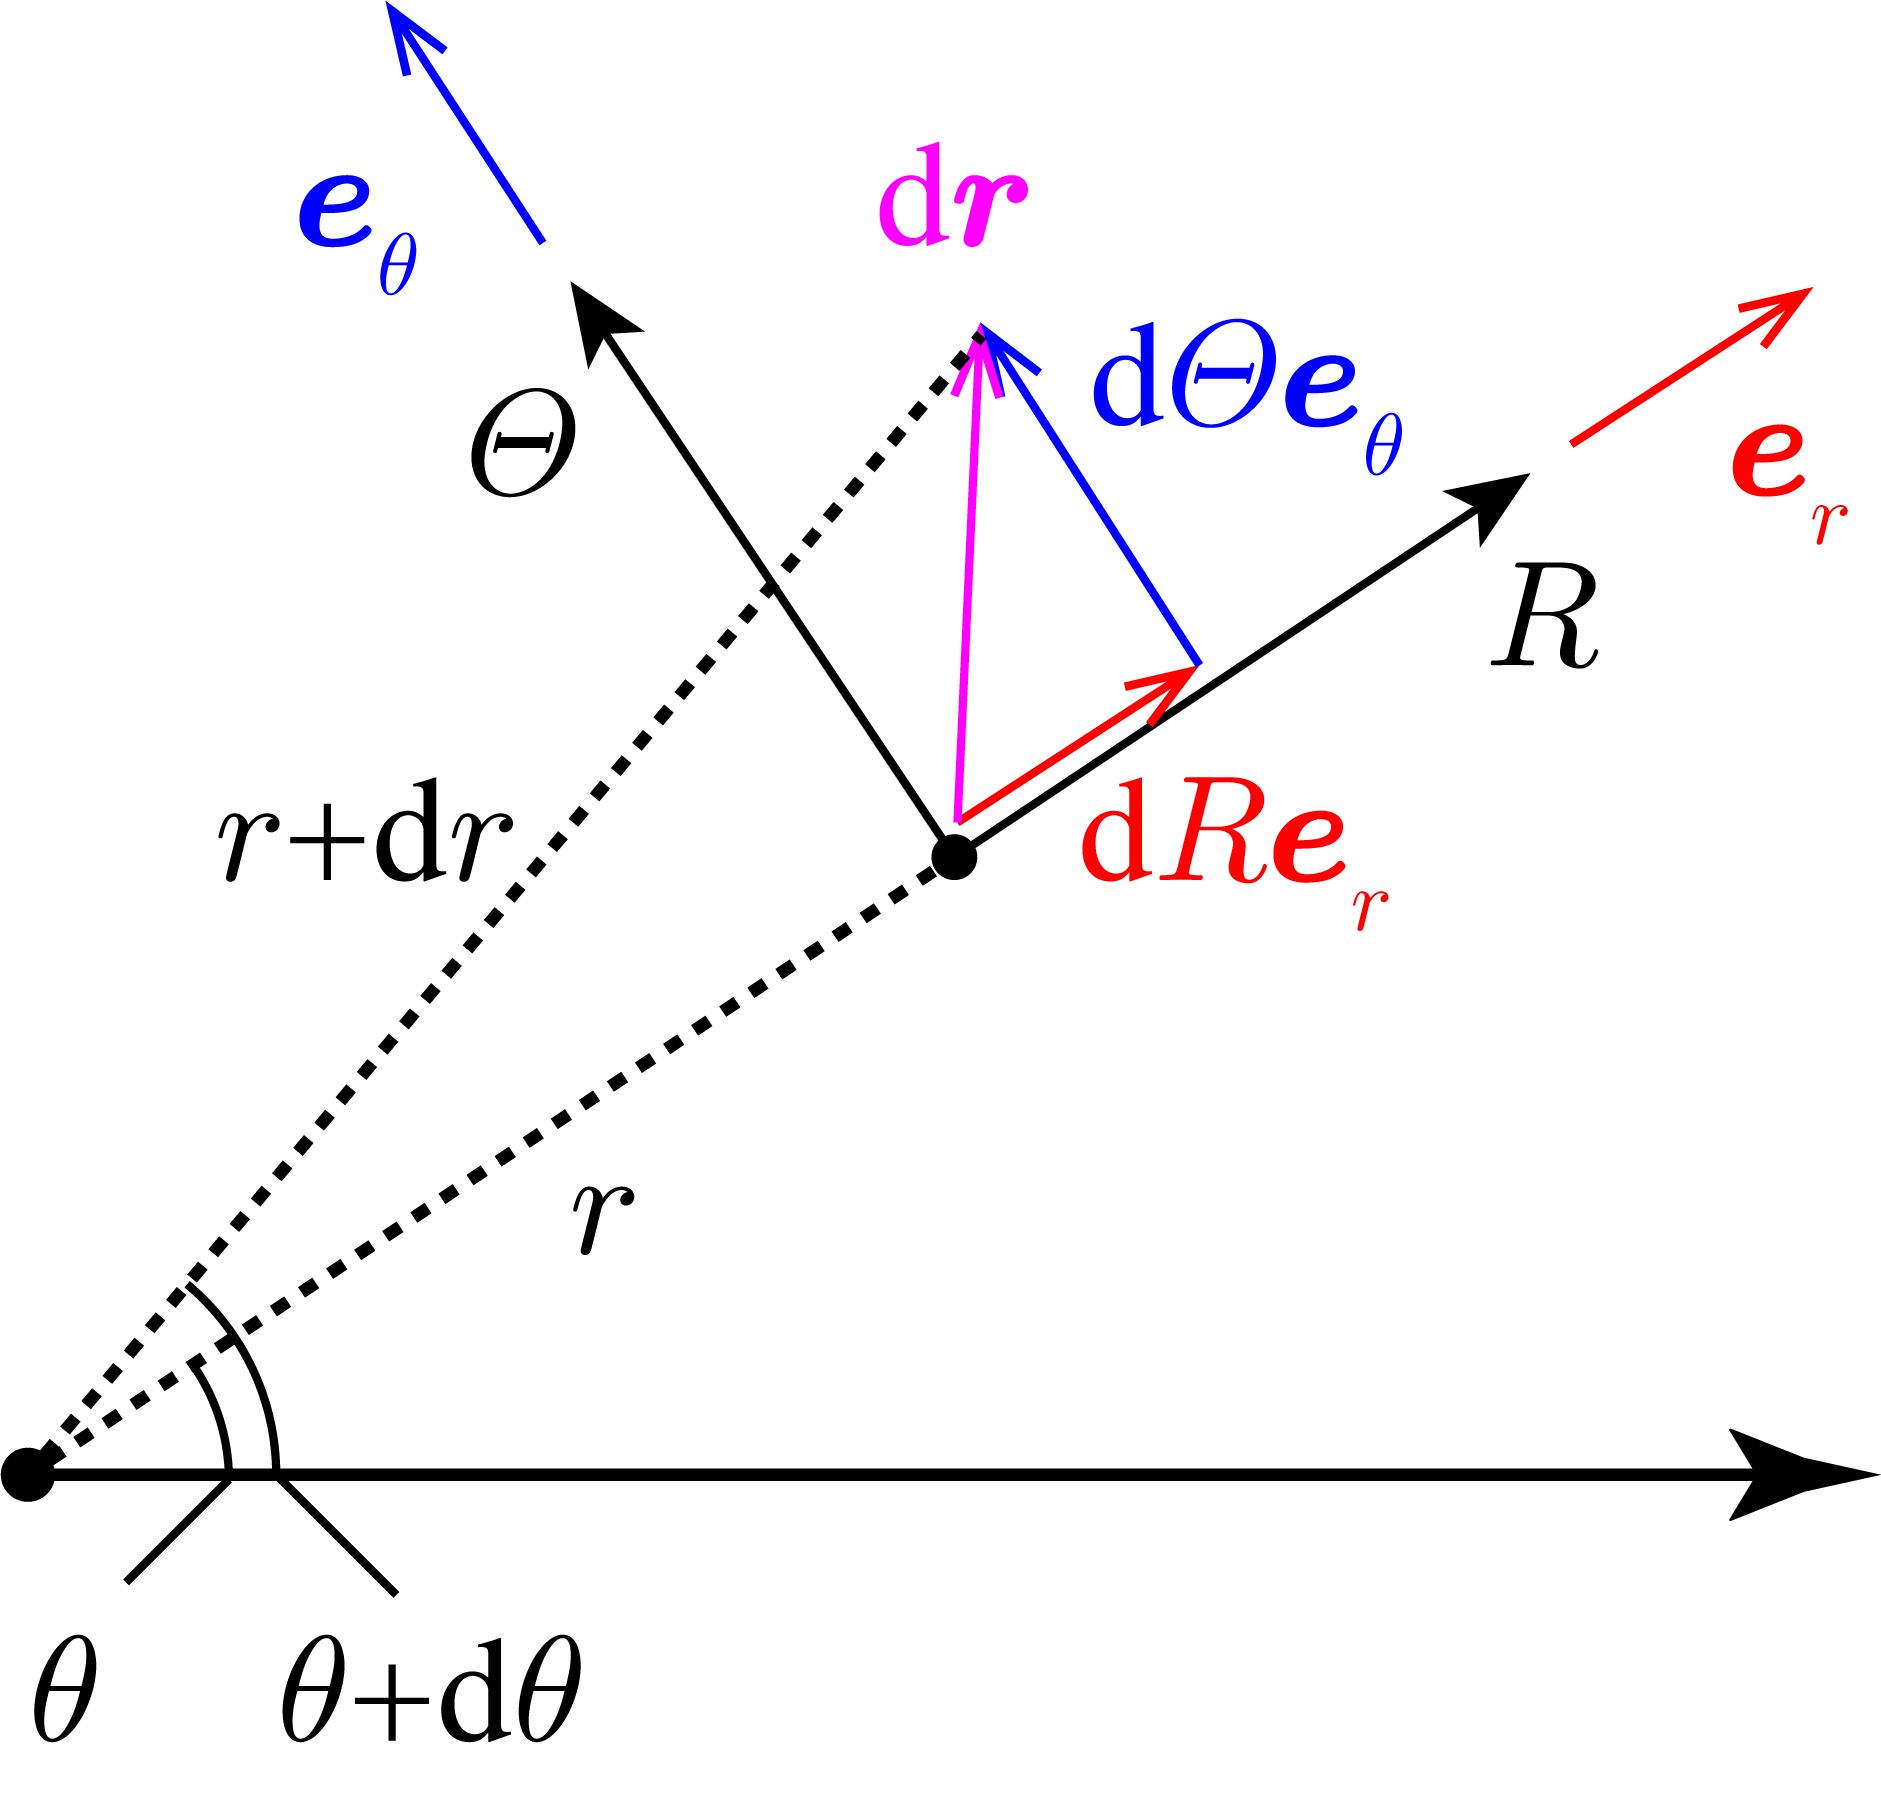
\includegraphics[width=6cm]{image/6-1-6.png}
\caption{极坐标系的活动框架}
\end{wrapfigure}
但这就较难求解\footnote{有兴趣的读者可以挑战一下.}.\,那么如果采用极坐标系会为我们带来何种新的思路呢?

那就是\emph{活动标架}(moving frame)的引入.\,无论粒子在何处,\,粒子的$\bs{r}$一定是作为了$r$和$\theta$的函数的.\,那么可以在粒子所在的点沿两个方向建立局域的$R-\varTheta$直角坐标系.\,这两个方向怎么确定呢?\,其实就是基矢的方向:
\[\bs{e}_r:=\frac{\partial\bs{r}}{\partial r}\left/\middle|\frac{\partial\bs{r}}{\partial r}\right|=\frac{\partial\bs{r}}{\partial r}\quad,\quad \bs{e}_\theta:=\frac{\partial\bs{r}}{\partial \theta}\left/\middle|\frac{\partial\bs{r}}{\partial \theta}\right|=\frac{1}{r}\frac{\partial\bs{r}}{\partial \theta}\]

上式中后一个偏导数的模为$r$是显然的.\,只需要考虑到圆的弧长和半径的关系即可.

局域的标架给我们什么方便?\,我们由偏导数和全微分的法则可以描述局域物体的微小位移.\,本质上,\,这相当于$\ud r$和$\ud \theta$导致的位矢$\bs{r}$改变$\ud \bs{r}$:
\[\ud \bs{r}_{(\ud r,\,\ud \theta)}=\ud \bs{r}_{(\ud r,\,0)}+\ud \bs{r}_{(0,\,\ud \theta)}=\ud R\bs{e}_r+\ud \varTheta\bs{e}_\theta\]
\[\ud \bs{r}_{(\ud r,\,\ud \theta)}=\frac{\partial \bs{r}}{\partial r}\ud r+\frac{\partial \bs{r}}{\partial \theta}\ud \theta=\ud r\bs{e}_r+r\ud \theta \bs{e}_\theta\]
\[\Rightarrow \quad \ud R=\ud r\;,\;\ud \varTheta=r\ud \theta\]

可见在曲线坐标情形下坐标的改变量$\ud r,\,\ud \theta$与在对应质点位移方向走过的弧长$\ud R,\,\ud \varTheta$的值一般是不一样的.\,它们之前的比值(弧长/坐标变化)称作\emph{拉梅系数}(Lam\'e coefficient).

\vspace{0.5cm}
既然叫做活动标架法,\,那么显然随着粒子的运动,\,两个基矢$\bs{e}_r,\,\bs{e}_\theta$的方向也在不断改变中.\,我们用极坐标,\,就是把一个物理量$\bs{A}$分解到粒子运动的瞬时局域坐标系中:
\[\bs{A}=A_r\bs{e}_r+A_\theta\bs{e}_\theta\]

那么在粒子发生运动后,\,以上矢量的改变应当由四部分组合而成:
\[\ud \bs{A}=\ud'\bs{A}+\tilde{\ud}\bs{A} \]
\[\ud' \bs{A}:=\ud A_r\bs{e}_r+\ud A_\theta\bs{e}_\theta\]
\[\tilde{\ud}\bs{A}:= A_r\ud\bs{e}_r+ A_\theta\ud\bs{e}_\theta\]

其中$\ud'$表示相对变化,\,类似于选取跟随旋转的活动标架而旋转的参考系后,\,矢量的变化量,\,故基矢自己的变化是被无视了的.\,而原来的$\ud$才表示绝对的变化.\,而$\tilde{\ud}$所带来的变化称作牵连变化或随体变化.\,它是即使前面的相对变化为零也会带来的,\,由于标架的``拉拽''导致的旋转带来的改变.\,事实上很容易证明其中的:
\[\ud \bs{e}_r=\ud \bs{\theta}\times \bs{e}_r=+\ud \theta \bs{e}_\theta\]
\[\ud \bs{e}_\theta=\ud \bs{\theta}\times \bs{e}_\theta=-\ud \theta \bs{e}_r\]

其中$\ud \bs{\theta}$是方向垂直于纸面向外的,\,大小即极坐标下物体坐标之角坐标的增量$\ud \theta$.

这就足以给出:
\[(\ud \bs{A})_r=\ud A_r-A_\theta \ud \theta\]
\[(\ud \bs{A})_\theta=\ud A_\theta+A_r \ud \theta\]
\newpage
两边再同时除以时间,\,我们得到粒子运动过程中一个矢量导数的两个分量与这矢量两个分量的导数之间的关系:
\[(\dot{\bs{A}})_r=\dot{A_r}-\dot{\theta}A_\theta\]
\[(\dot{\bs{A}})_\theta=\dot{A_\theta}+\dot{\theta}A_r\]

导数的分量不等于分量的导数,\,这也是坐标系的弯曲所带来的.\,数学上,\,这意味算符$\partial_t$与算符$\bs{e}\cdot$的\emph{不对易性}(non-commutative):
\[\bs{e}\cdot(\partial_t \bs{A})\neq \partial_t(\bs{e}\cdot \bs{A})\]

通过这个原理,\,我们可以推理得到:
\[\bs{r}=r\bs{e}_r+0\bs{e}_\theta\quad \Rightarrow\quad r_r=r\,,\,r_\theta=0\]
\[\bs{v}=\dot{\bs{r}}\quad \Rightarrow\quad  v_r=\dot{r_r}-\dot{\theta}r_\theta=\dot{r}\,,\,v_\theta=\dot{r_\theta}+\dot{\theta}r_r=\dot{\theta}r\]
\[\bs{a}=\dot{\bs{v}}\quad \Rightarrow\quad  a_r=\dot{v_r}-\dot{\theta}v_\theta=\ddot{r}-\dot{\theta}^2r\,,\,a_\theta=\dot{v_\theta}+\dot{\theta}v_r=\ddot{\theta}r+2\dot{\theta}\dot{r}\]

这个操作甚至可以继续下去,\,计算急动度等:
\[\bs{j}=\dot{\bs{a}}\quad \Rightarrow \quad j_r=\dot{a_r}-\dot{\theta}a_\theta=\dddot{r}-3\dot{\theta}\ddot{\theta}r-3\dot{\theta}^2\dot{r}\,,\,j_\theta=\dot{a_\theta}+\dot{\theta}a_r=\dddot{\theta}r+3\ddot{\theta}\dot{r}+3\dot{\theta}\ddot{r}-\dot{\theta}^3r\]
\[\cdots\]

极坐标下速度,\,加速度的公式是非常常用的,\,它们是:
\[\bs{v}=(\dot{r}\,,\,\dot{\theta}r)\quad\bs{a}=(\ddot{r}-\dot{\theta}^2r\,,\,\ddot{\theta}r+2\dot{\theta}\dot{r})\]

故,\,在之前的首尾相追问题\ref{6-1-5}中以正方形中心为原点,\,以初始位置为极轴方向建立极坐标系.\,那么两个条件:\,速度大小恒定为$v$和位矢速度夹角恒定$3\pi/4$表述为:
\[v_r^2+v_\theta^2=v^2\quad ,\quad \frac{v_\theta}{v_r}=-1\]

相当容易解出来两个分速度的值,\,再结合之前的速度公式:
\[\dot{r}=-\frac{\sqrt{2}}{2}v\quad ,\quad \dot{\theta}r=\frac{\sqrt{2}}{2}v\]

这样,\,便可以轻松解出运动方程来,\,结合初始条件,\,不妨设初始矢径为$r_0$,\,幅角为$0$:
\[\dot{r}=-\frac{v}{\sqrt{2}}\quad \Rightarrow \quad r=r_0-\frac{vt}{\sqrt{2}}\]
\[\dot{\theta}=\frac{v}{\sqrt{2}r_0-vt}\quad \Rightarrow \quad  \theta =-\ln\left(1-\frac{vt}{\sqrt{2}r_0}\right)\]

轨迹方程通过上述方程消参即可.\,但也可以通过之前的微分方程相除得到新微分方程求解,\,曲线为\emph{对数螺线}(logarithmic spiral):
\[\frac{\ud r}{\ud \theta}=-r\quad \Rightarrow \quad r=r_0\ue^{-\theta}\]

平面的极坐标系在三维空间的推广为\emph{柱坐标系}(cylindrical coordinate system)和\emph{球坐标系}(spherical coordinate system).\,类似公式的核心也与平面极坐标相差无几,\,都在于活动标架的基矢微分.\,请读者自行推导.

\vspace{0.2cm}
{\bf 3.\,自然坐标系下的分解}

设想仍然采用活动标架法的思路,\,但是,\,标架的方向不再由粒子的位置相对事先建立的背景的坐标系的关系而决定.\,而是紧密地由粒子运动的性质:\,瞬时的速度方向,\,轨迹曲线的弯曲方向等决定.\,那么我们就得到了特殊的标架:\,\emph{自然坐标系}(natural coordinates).

自然坐标系的建立是派生于粒子运动的轨迹的那条曲线的性质的.\,借助牛顿等人创立的微积分与笛卡尔等人创立的解析几何的帮助,\,对于光滑曲线曲面的性质的研究构成了\emph{古典微分几何}(classical differential geometry)的主要课题.\,

我们考虑三维空间问题.\,对于一条空间曲线.\,它总是一些点的集合,\,而如果规定某个起始点以后,\,每一个点都会有一个$s$坐标,\,它就是从起始点到这个点的弧长.\,而其实我们可以把$s$视作一个自变量,\,因为$s$改变而改变的是不同点的位置$\bs{r}$.\,也就是说$\bs{r}(s)$作为了$s$的函数.\,那么这个曲线在某一点处的切矢量就可以被自然地定义为:
\[\bs{\tau}=\frac{\ud \bs{r}}{\ud s}\]

\begin{wrapfigure}[14]{o}[-10pt]{6cm}\label{6-1-7}
\vspace{-0.2cm}
\centering
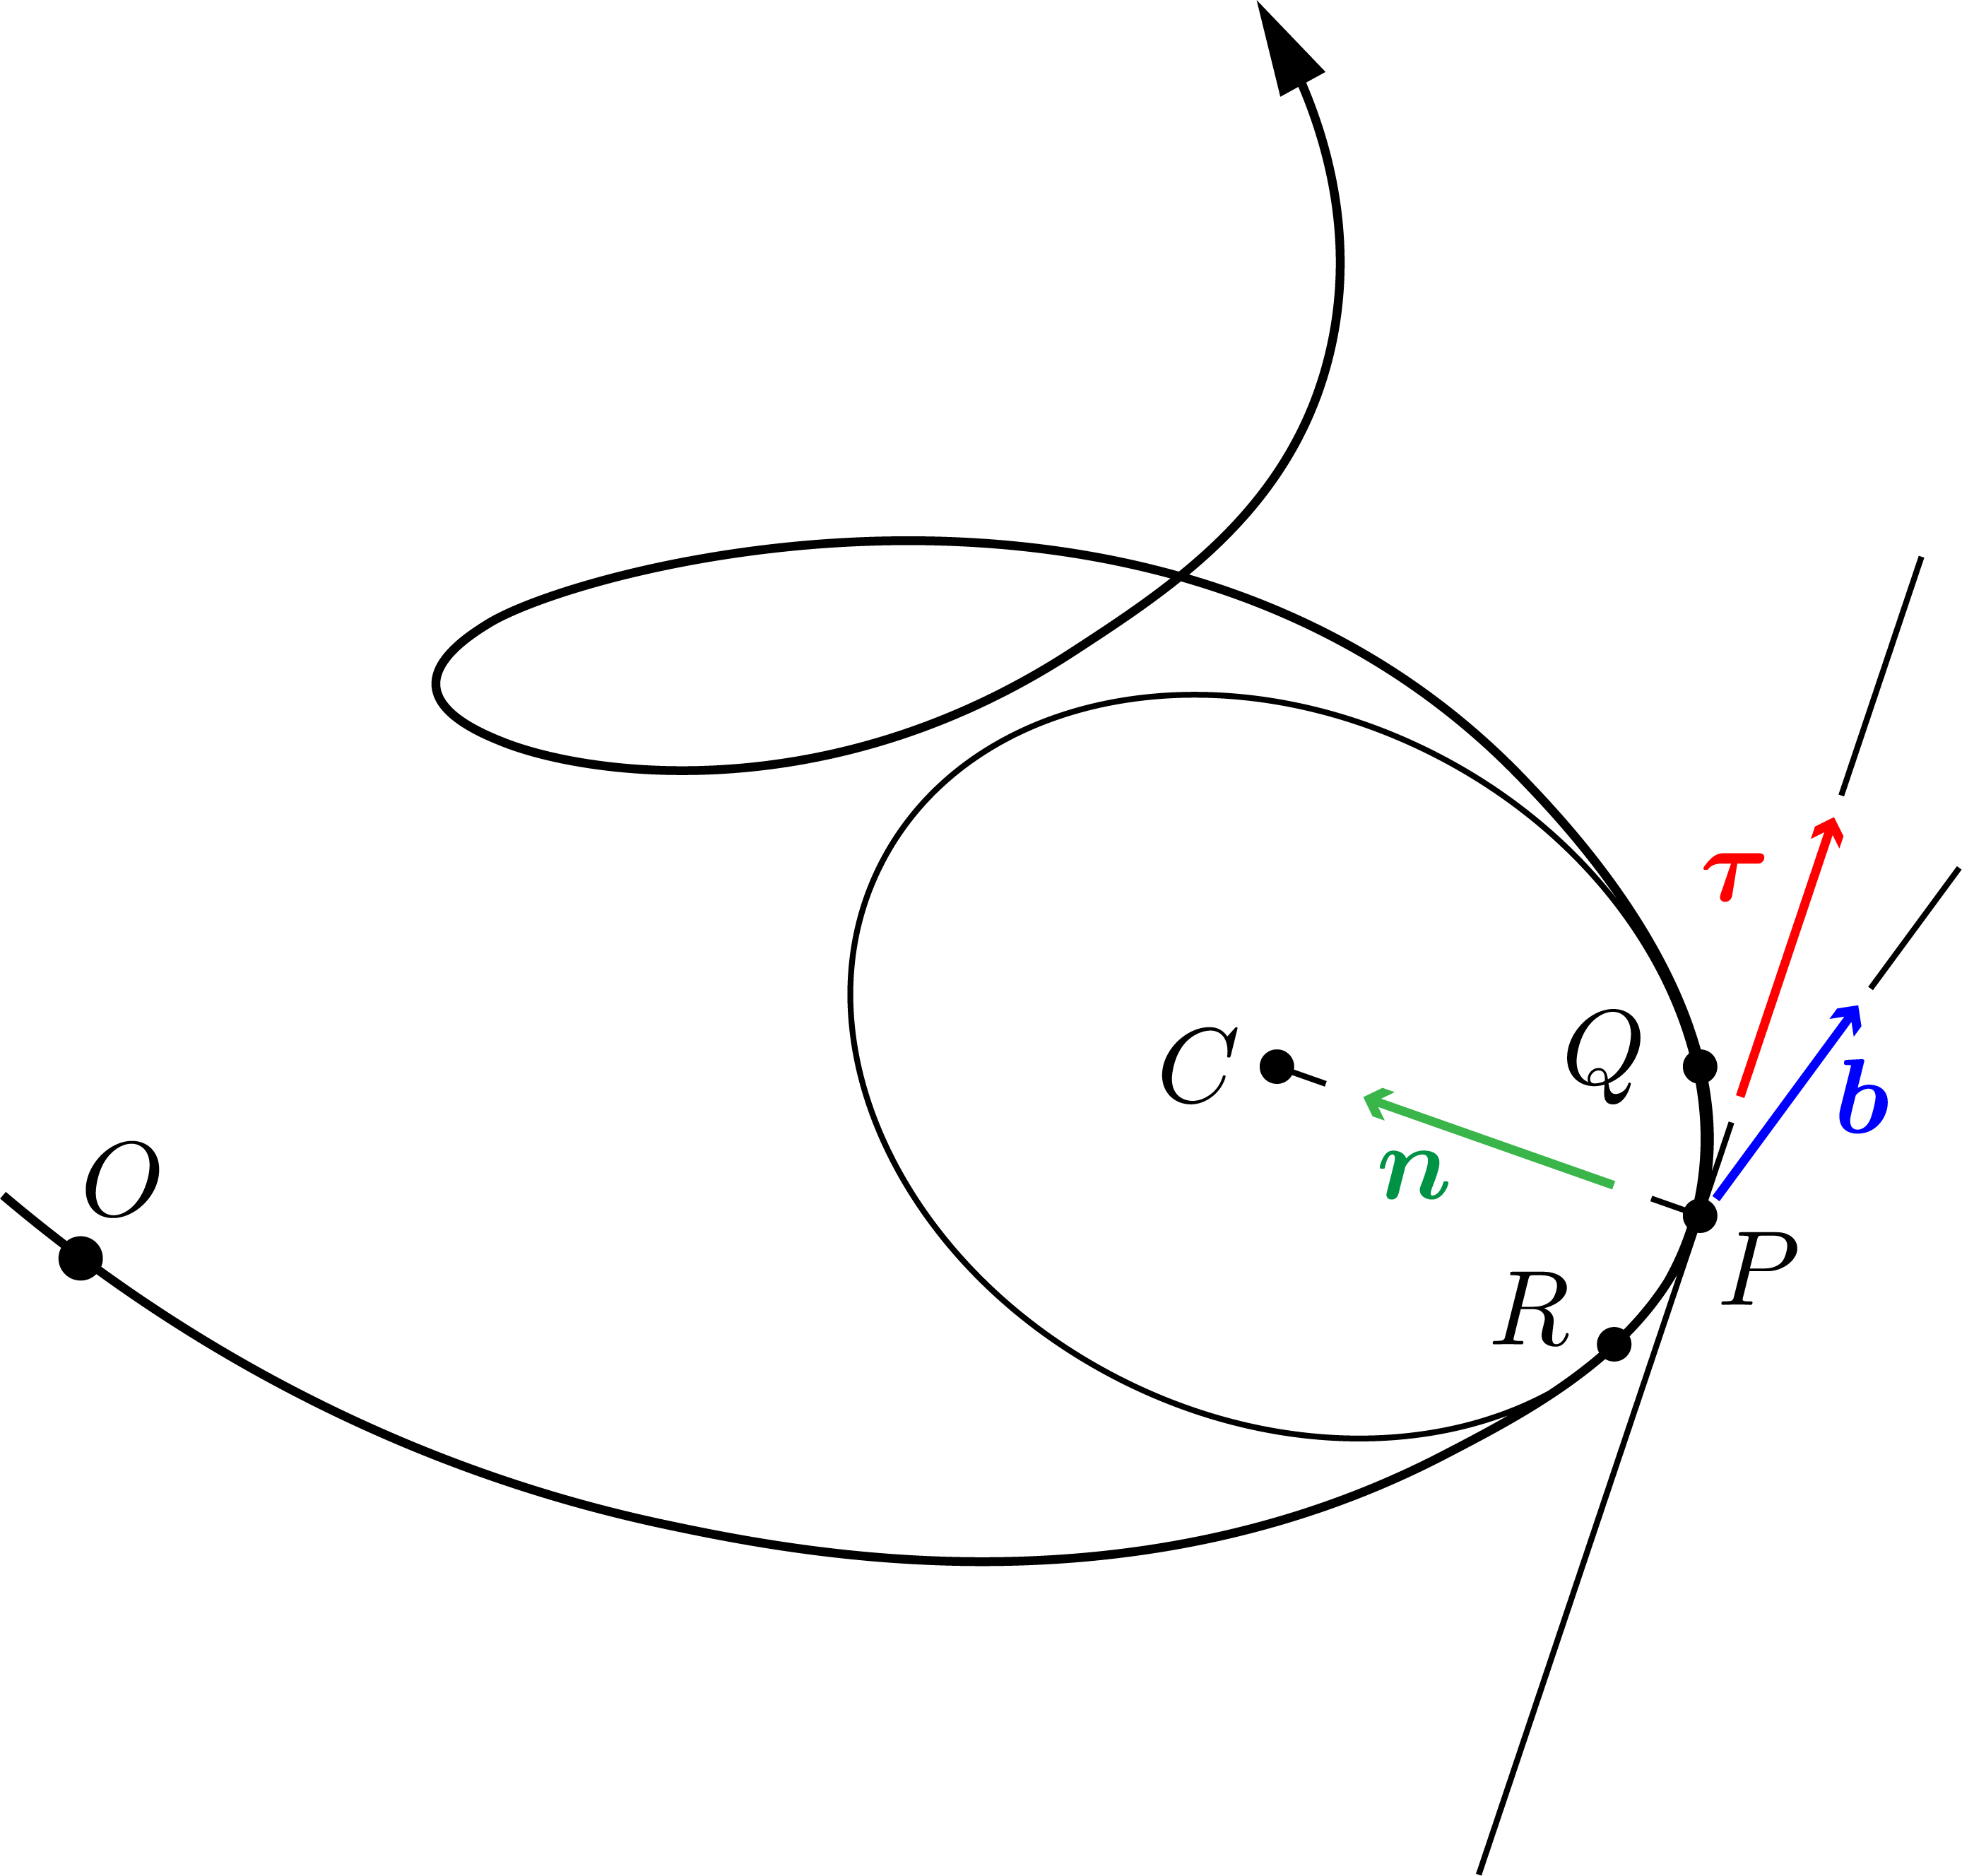
\includegraphics[width=6cm]{image/6-1-7.png}
\caption{Frenet框架}
\end{wrapfigure}
以上矢量模自然为$1$.\,因为分子$\ud \bs{r}$的长度就是分母的$\ud s$.\,方向则是在曲线的\emph{切线}(tangent line)方向.\,切线是这样一种线:\,曲线上有一点$P$.\,如果在$P$两侧任取一个点$Q$并连接$PQ$,\,使$Q$无限接近$P$即$\ud s \to 0$,\,那么$PQ$所在的直线的极限就是$P$点的切线.\,这又引申出第二个概念:\,如果在$P$所有各取一个点$Q,\,R$.\,那么$PQR$三点确定的圆也将随着$Q,\,R$同时无限接近于$P$而具有极限.\,这个圆叫做\emph{密切圆}或\emph{曲率圆}(osculating circle).\,其所在的平面叫做\emph{密切平面}(osculating plane).\,而圆心$C$为\emph{曲率中心}(center of curvature),\,最后,\,实际上$P$到$C$的方向就是\emph{法}(normal)方向,\,该方向的单位矢量叫做法矢量$\bs{n}$.\,而副法矢量$\bs{\tau}\times\bs{n}=\bs{\beta}$所决定的方向为\emph{副法}(binormal)方向.\,这样三个矢量便构成\emph{弗雷内框架}(Frenet frame)或称TNB框架.

事实上,\,如果计算曲线在过程中的转向,\,它可以用三个矢量方向的变化来表示.\,如果计算三个矢量对$\ud s$的变化率,\,一定能写作:
\[\begin{array}{rlll}
\frac{\ud \bs{\tau}}{\ud s}=		&	+0\bs{\tau} 	&	+k\bs{n} 		& +\varepsilon\bs{\beta}\\
\frac{\ud \bs{n}}{\ud s}=		&	-k\bs{\tau} 	&	+0\bs{n} 		& +\gamma\bs{\beta}\\
\frac{\ud \bs{\beta}}{\ud s}=		&	-\varepsilon\bs{\tau} 	&	-\gamma\bs{n} 		& +0\bs{\beta}
\end{array}\]

这是因为框架一定要具有正交归一的一套基矢量,\,而且这个性质在曲线上任何一点都要成立,\,指的是以下六个式子:
\[\bs{\tau}\cdot\bs{\tau}=1\quad,\quad\bs{n}\cdot\bs{n}=1\quad,\quad \bs{\beta}\cdot\bs{\beta}=1\]
\[\bs{\tau}\cdot\bs{n}=0\quad,\quad\bs{n}\cdot\bs{\beta}=0\quad,\quad \bs{\beta}\cdot\bs{\tau}=0\]

对六个式子分别求导数就看出来了,\,\emph{一个单位矢量自己的导数必然垂直于自身},\,从而三个基矢导数在自己上的投影都必须为零.\,而两个不同基矢的导数互相在对方方向的投影则会正负相消,\,这样才能保证两个矢量始终正交.\,就能理解之前的$9$个系数为什么要写成这个形式.

最后我们指出,\,系数$\varepsilon$应当是$0$.\,这是因为作为法线方向的定义本身,\,它就应当在$\bs{\tau}$的变化量$\ud\bs{\tau}$所在的方向上.\,从而第一个式子不会具有$\bs{\beta}$方向的分量.\,综上所述,\,我们得到了:

\[\begin{array}{rlll}
\frac{\ud \bs{\tau}}{\ud s}=		&	 	&	+k\bs{n} 		& \\
\frac{\ud \bs{n}}{\ud s}=		&	-k\bs{\tau} 	&	 		& +\gamma\bs{\beta}\\
\frac{\ud \bs{\beta}}{\ud s}=		&	 	&	-\gamma\bs{n} 		& 
\end{array}\]

这就是\emph{弗雷内公式}(Frenet formulae).\,其中$k$称作曲线的\emph{曲率}(curvature).\,它的意义是衡量了曲线方向转动的快慢,\,事实上由于曲线切线的无穷小转动角度其实在竖直上恰好会等于无穷小矢量$\ud\bs{\tau}$的长度,\,从而有:
\[k=\abs{\frac{\ud\bs{\tau}}{\ud s}}=\frac{\ud\theta}{\ud s}\]

即,\,曲率为:\,质点沿曲线走单位长度所转过的角度.\,曲率半径实际上是曲率的倒数.\,它是曲率圆的半径$\rho=1/k$.

而$\gamma$则被称作\emph{挠率}(torsion).\,我们通过弗雷内公式的第三式可以发现,\,挠率反映了副法矢量,\,或者说被复法矢量作为法平面的密切平面,\,绕曲线此时的切线的旋转快慢.\,它使得粒子瞬时运动的那个平面在改变着.\,下面我们会发现,\,实际上挠率对运动学中直到加速度的表达式都是没有任何贡献的.

如何用自然法描述粒子的运动?\,事实上这就相当于把粒子运动的路程$s$和三个矢量$\bs{\tau},\,\bs{n},\,\bs{\beta}$都表示为时间的函数:
\[s(t),\,\bs{\tau}(t),\,\bs{n}(t),\,\bs{\beta}(t)\]

但事实上,\,曲线本身轨迹必须先存在才能让我们事先确定好框架,\,而这样一个曲线其实本身由$\bs{r}(s)$给出,\,而且满足:
\[\frac{\ud \bs{r}}{\ud s}=\bs{\tau}\quad,\quad \frac{\ud^2 \bs{r}}{\ud s^2}=k\bs{n}\quad,\quad \frac{\ud^3 \bs{r}}{\ud s^3}=-k^2\bs{\tau}+\frac{\ud k}{\ud s}\bs{n}+k\gamma\bs{\beta}\]

然后我们唯一要做的就是给出$s(t)$函数,\,这一定可以帮助我们确定运动的各个量.

事实上,\,由于泰勒展开公式,\,近似到三阶:
\[\Delta \bs{r}\simeq\frac{\ud \bs{r}}{\ud s}\ud s+\frac{1}{2}\frac{\ud^2 \bs{r}}{\ud s^2}\ud s^2+\frac{1}{6}\frac{\ud^3 \bs{r}}{\ud s^3}\ud s^3=(k\ud s-\frac{k^2}{6}\ud s^3)\bs{\tau}+(\frac{k}{2}\ud s^2+\frac{1}{6}\frac{\ud k}{\ud s}\ud s^3)\bs{n}+\frac{k\gamma}{6}\ud s^3\bs{\beta}\]

如果只保留领头项,\,忽略高阶小量.\,我们就得到,\,在粒子运动的局域坐标系中,\,位移$\ud s$长度到达的点三个坐标$T,\,N,\,B$分别近似为:
\[T=\ud s \quad,\quad N=\frac{k}{2}\ud s^2 \quad,\quad B=\frac{k\gamma}{6}\ud s^3\]

仍然考虑之前的三阶近似下的严格$\Delta \bs{r}$与$\ud{s}$的关系,\,这一次代入$s(t)$的三阶套了展开:
\[\ud s\simeq \dot{s}\ud t+\frac{\ddot{s}}{2}\ud t^2+\frac{\dddot{s}}{6}\ud t^3\]

我们整理$\ud t$的各阶项,\,最终得到:
\[\Delta \bs{r}\simeq \bs{v}\ud t+\frac{1}{2}\bs{a}\ud t^2+\frac{1}{6}\bs{j}\ud t^3\]

其中速度与加速度的公式为:
\[\bs{v}=\dot{s}\bs{\tau}\]
\[\bs{a}=\ddot{s}\bs{\tau}+k\dot{s}^2\bs{n}\]

速度方向必然沿切向,\,大小上就等于$\dot{s}$,\,即单位时间走过的弧长.\,而加速度则有两个分量.\,一是由于速率在增减导致的切向加速度,\,大小等于$a_\tau=\ddot{s}$;\,第二项则是由于曲线的弯曲导致的法向加速度.\,它的值为$a_n=\dot{s}^2/\rho$.\,

如果要计算急动度等,\,可以从之前的泰勒展示中获得,\,其实还可以直接对加速度求导数,\,此时表达式会突然产生很多项:
\[\bs{j}=(\dddot{s}-k^2\dot{s}^3)\bs{\tau}+(3k\dot{s}\ddot{s}+\dot{k}\dot{s}^3)\bs{n}+k\gamma\dot{s}^3\bs{\beta}\]

利用自然坐标下的分解方式,\,如果已经直到特定曲线的曲率,\,就可以根据质点在曲线上的运动方式来计算运动的加速度.\,但是反过来利用运动学公式来确定曲线的曲率半径也不失为一种极其简单的做法.\,我们注意到,\,利用加速度在垂直于速度方向的那个分量即为$v^2/\rho$的结论,\,可以得到:
\[\rho=\frac{\bs{v}^3}{\abs{\bs{a}\times\bs{v}}}\]

例如,\,如果已知二维空间中的曲线方程$y=f(x)$.\,那么如果命一质点在曲线上运动且满足$x=t,\,y=f(t)$,\,那么速度为$\bs{v}=(1,\,f')$,\,加速度为$\bs{a}=(0,f'')$.\,利用上式可得:
\[\rho=\frac{(1+f'^2)^\frac{3}{2}}{\abs{f''}}\]

再例如.\,之前的首尾相追问题中,\,曲线对数螺线写作:
\[r=a\ue^{k\theta}\]

如何计算曲率半径?\,我们让粒子在曲线上绕极点做匀速旋转,\,也就是:
\[\theta=\omega t\quad,\quad r=a\ue^{k\omega t}\]

那么借助极坐标的加速度公式得:
\[\bs{v}=(\dot{r},\,\dot{\theta}r)=(k\omega a\ue^{k\omega t},\,\omega a\ue^{k\omega t})=(k\omega r,\,\omega r)\]
\[\bs{a}=(\ddot{r}-\dot{\theta}^2r,\,\ddot{\theta}r+2\dot{\theta}\dot{r})=((k^2-1)\omega^2 a\ue^{k\omega t},\,2k\omega^2 a\ue^{k\omega t})=((k^2-1)\omega^2 r,\,2k\omega^2 r)\]

代入之前的曲率公式便可以得到:
\[\rho=\sqrt{1+k^2}r\]

\subsection{刚体的运动}

关于刚体的运动,\,它的定义我们其实将在之后的刚体专门的章节又一次做更进一步的探讨.\,初步我们认为所谓刚体就是这样一种物体:\,存在一个特殊的参考系(平动或转动)能够使得该物体上每一个点都每时每刻相对静止.\,但是这样我们又涉及到下一节才讲的参考系的概念.\,在此我们又不得不早于预期提及.

\begin{wrapfigure}[12]{o}[-10pt]{6cm}\label{6-1-8}
\vspace{-0.2cm}
\centering
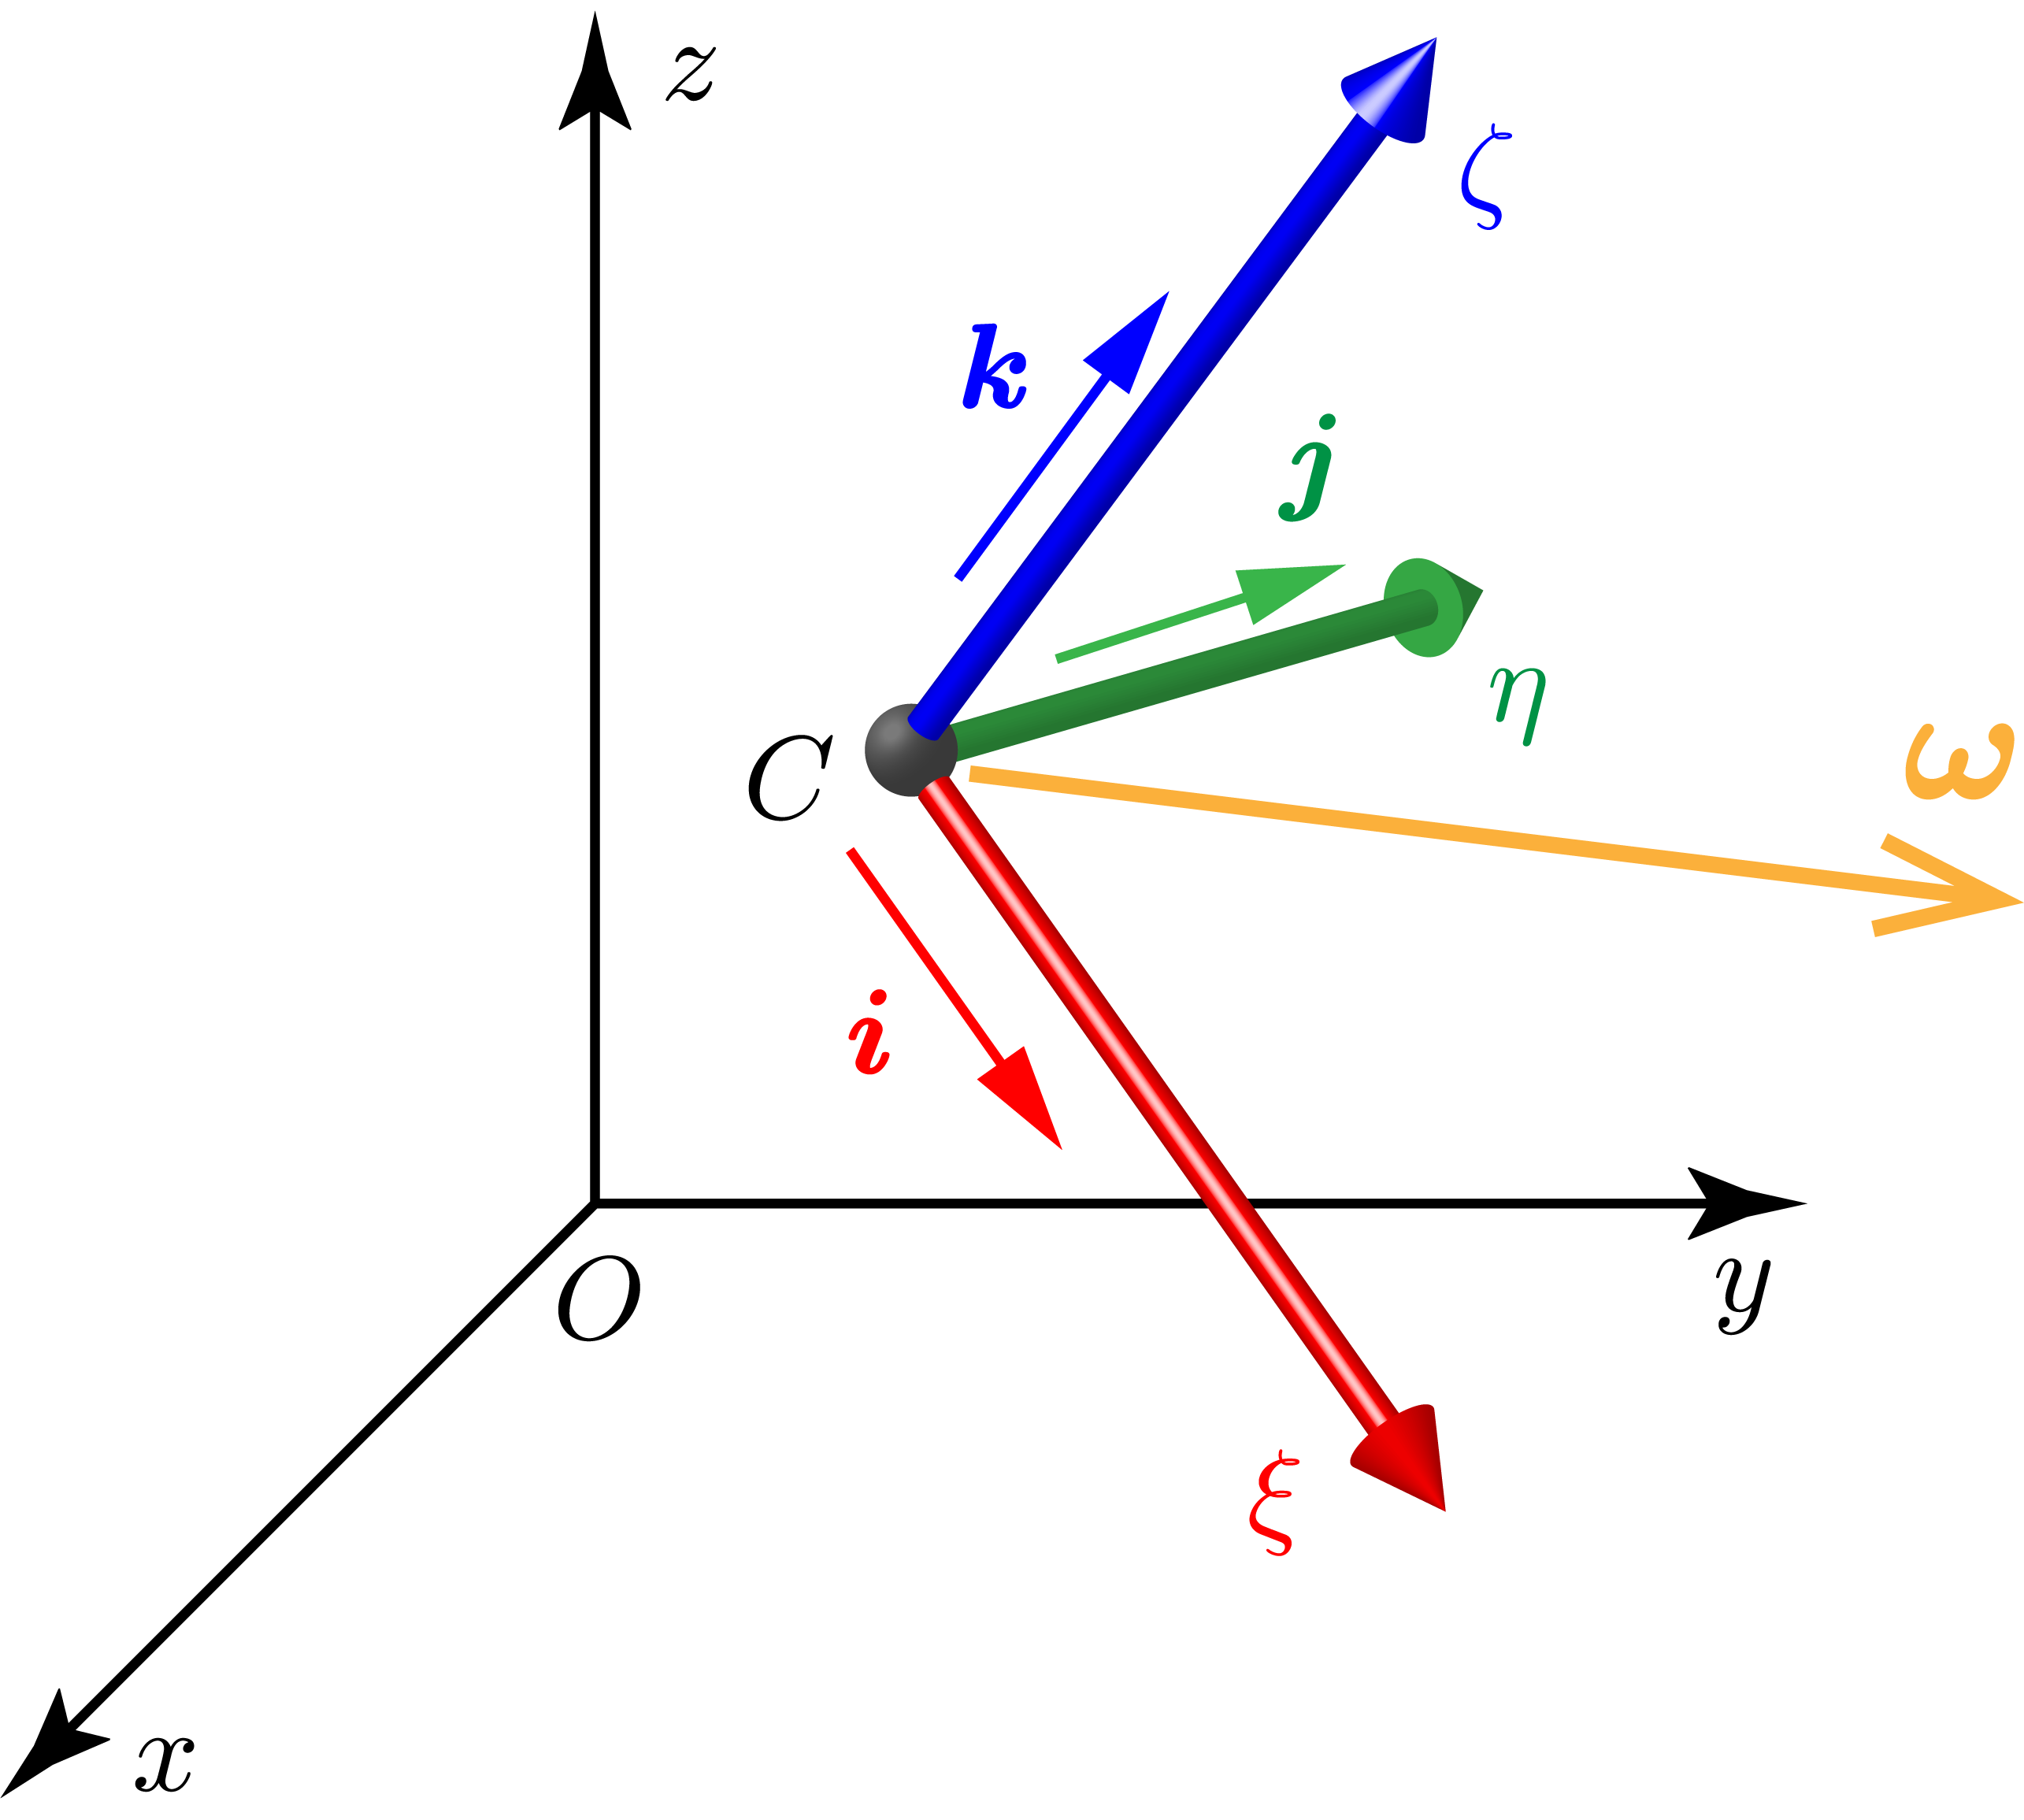
\includegraphics[width=6cm]{image/6-1-8.png}
\caption{刚体的本征框架}
\end{wrapfigure}
为此我们换一种更加直观的方式引入这些概念而不是去严格定义刚体与参考系的概念.\,设想我们有一个正交的刚性框架,\,即三条射线状坐标轴构成的物体,\,下称$\xi,\,\eta,\,\zeta$轴,\,该框架就会自然造成四个矢量.\,首先是框架原点$C$的位置矢量$\bs{r}$.\,其次是三坐标轴方向的三个基矢\footnote{原来的基矢方向记做$\bs{e}_{x,\,y,\,z}$.}$\bs{i},\,\bs{j},\,\bs{k}$.\,它们都会随着时间变化,\,可以用四个导数表征.\,其中$\bs{v}=\dot{\bs{r}},\,\bs{a}=\ddot{\bs{r}}$.\,但是,\,对于三个基矢导数有没有更加简单的描述方法呢?\,如果我们把三个基矢导数就向三个基矢本来的方向分解\footnote{由于字母$i,\,j$上本来就有点,\,所以在符号上约定遇到要在这两个字母上加点时改为横向$\ddot{\imath},\,\ddot{\jmath}$.\,偶尔也见到反而去掉点的$\imath,\,\jmath$.\,出于这样无法表示高阶导数,\,我们不采用这种模式.}:
\[\begin{array}{rlll}
\bs{\ddot{\imath}}=		&	+\omega_{11}\bs{i} 	&	+\omega_{12}\bs{j} 		& +\omega_{13}\bs{k}\\
\bs{\ddot{\jmath}}=		&	+\omega_{21}\bs{i} 	&	+\omega_{22}\bs{j} 		& +\omega_{23}\bs{k}\\
\bs{\dot{k}}=				&	+\omega_{31}\bs{i} 	&	+\omega_{32}\bs{j} 		& +\omega_{33}\bs{k}
\end{array}\]

依然,\,我们注意到出于以下正交归一的结构不会改变,\,在求导下为零,\,所以上述表达式中的九个系数反对称:
\[\frac{\ud}{\ud t}\left\{\begin{array}{cccc}
1= 	&\bs{i}\cdot\bs{i} 	&\bs{j}\cdot\bs{j} 	&\bs{k}\cdot\bs{k} 	\\
0= 	&\bs{i}\cdot\bs{j} 	&\bs{j}\cdot\bs{k} 	&\bs{k}\cdot\bs{i}
\end{array}\right\}=0\quad \Rightarrow \quad\omega_{ij}+\omega_{ji}=0\]

出于某种符号约定与对称的原因,\,我们把导数重新写作:
\[\begin{array}{rlll}
\bs{\ddot{\imath}}=		&									 	&	+\omega_3\bs{j} 				& -\omega_2\bs{k}\\
\bs{\ddot{\jmath}}=		&	-\omega_3\bs{i} 			&									 		& +\omega_1\bs{k}\\
\bs{\dot{k}}=				&	+\omega_2\bs{i} 			&	-\omega_1\bs{j} 				& 
\end{array}\]

这样,\,如果我们定义一个矢量:
\[\bs{\omega}=\omega_1\bs{i}+\omega_2\bs{j}+\omega_3\bs{k}\]

就能够造成:
\[\bs{\ddot{\imath}}=\bs{\omega}\times \bs{i}\quad ,\quad \bs{\ddot{\jmath}}=\bs{\omega}\times \bs{j}\quad ,\quad \bs{\dot{k}}=\bs{\omega}\times \bs{k}\]

这就是刚体的\emph{角速度}(angular velocity)矢量.\,用它可以计算刚体中的各种转动的物理量.

具体来说,\,什么叫做刚体?\,事实上以上三个坐标轴本身就构成了刚体,\,或者是某刚体的一部分.\,如果有一个空间点每时每刻向杆坐标系的三个坐标面引三垂线,\,三个坐标都始终保持常数,\,那么就说这个空间点是\emph{固连}(fixed)在该坐标系中的.\,而如果一个物体上的每一个点都固连带该坐标系中,\,那么相对这个坐标系该物体就无法发生形变,\,从而这就是一个刚体.\,这种情况下,\,刚体与坐标系就存在一个相互关系,\,这个坐标系是由刚体所对应的固连坐标系,\,而坐标系本身又可以视作某种不能变形的刚体.

我们在坐标系中找到固连在坐标系上的两个点,\,或者说在刚体上找到固连在刚体上的两个点(以后不加以区分).\,从一个点指向另一个点形成矢量$\bs{R}$,\,由于固连在坐标系中,\,这个矢量对坐标系造成的三个分量都是固定的,\,也就是$\bs{R}=R_1\bs{i}+R_2\bs{j}+R_3\bs{k}$中的$R_1,\,R_2,\,R_3$都是常数.\,那么这个矢量跟随坐标系而变化的导数就是:
\[\dot{\bs{R}}=R_1\bs{\ddot{\imath}}+R_2\bs{\ddot{\jmath}}+R_3\bs{\dot{k}}=\bs{\omega}\times(R_1\bs{i}+R_2\bs{j}+R_3\bs{k})=\bs{\omega}\times\bs{R}\]

在物理上,\,这就是说,\,任何固连在转动坐标系中的矢量$\bs{R}$都将以角速度$\bs{\omega}$跟随坐标系旋转,\,$\bs{\omega}$的方向就是瞬时转动轴,\,$\bs{\omega}$的大小就是旋转角速度大小.\,注意两点,\,一是这个角速度$\bs{\omega}$是全局的,\,无论矢量相对坐标系在任何位置,\,无论距离最初选取的坐标系中心有多远,\,只要固连在坐标系中,\,就会以完全一样的角速度矢量$\bs{\omega}$去改变$\dot{\bs{R}}=\bs{\omega}\times\bs{R}$.\,二是这个角速度作用在任何量纲上.\,无论是两个空间点之间的那个(位移)矢量,\,还是速度矢量,\,力矢量等等,\,任意量纲的矢量$\bs{A}$只要相对旋转坐标系具有固定的方向,\,在地面系中就会跟着坐标系一同旋转而具有导数:
\[\dot{\bs{A}}=\bs{\omega}\times\bs{A}\quad \text{for }\; \bs{A}\;\text{fixed in frame}\; C-\xi\eta\zeta\]

以后我们可以脱离坐标系而讨论刚体.\,为了研究刚体的运动,\,我们只需要在刚体上取一个合适的固连点$C$作为中心(类似于坐标系的原点),\,这个点叫做\emph{基点}(cardinal point).\,那么,\,不失一般性地,\,刚体的运动将用基点$C$的位置$\bs{r}(t)$和角速度$\bs{\omega}(t)$描述.\,譬如,\,为了求得某一时刻刚体上一点$P$的速度.\,我们可以找到从$C$指向$P$的矢量$\bs{R}$.\,那么,\,由于$\bs{r}_{OC}+\bs{r}_{CP}=\bs{r}_{OP}$.\,这就是说:
\[\bs{v}_{P}=\dot{\bs{r}}_{OP}=\dot{\bs{r}}_{OC}+\dot{\bs{r}}_{CP}=\bs{v}_{C}+\dot{\bs{R}}\]

最后再由之前的用角速度算导数的方法,\,得到著名的基点法速度表达式:
\[\bs{v}_{P}=\bs{v}_{C}+\bs{\omega}\times\bs{R}\]

即:\,刚体上一点速度等于跟随基点平动的速度$\bs{v}_{C}$加上绕基点以$\bs{\omega}$转动的速度$\bs{\omega}\times\bs{R}$的和.

至于加速度,\,只需要对上式再求一次导数$\dot{\bs{v}}_{P}=\dot{\bs{v}}_{C}+\dot{\bs{\omega}}\times\bs{R}+\bs{\omega}\times\dot{\bs{R}}$:
\[\bs{a}_{P}=\bs{a}_{C}+\bs{\beta}\times\bs{R}+\bs{\omega}\times(\bs{\omega}\times\bs{R})\]

即:\,刚体上一点速度等于跟随基点平动的加速度$\bs{a}_{C}$加上绕基点以$\bs{\beta}$转动的角向加速度$\bs{\beta}\times\bs{R}$,\,最后再加上由于速度$\bs{\omega}\times\bs{R}$本身也在绕轴以$\bs{\omega}$旋转带来的向轴加速度$\bs{\omega}\times(\bs{\omega}\times\bs{R})$的和.


\section{参考系变换}

\subsection{点变换}

事实上,\,对旋转坐标系的分析正如对刚体的分析那样,\,一个旋转坐标系的描述正由两点构成,\,一是这个参考系原点$C$的运动方程.\,给出它我们就可以求出任意时刻另一个参考原点的速度与加速度:
\[\bs{v}_C=\dot{\bs{r}}_C\quad,\quad \bs{a}_C=\ddot{\bs{r}}_C\]


\begin{wrapfigure}[14]{o}[-10pt]{6cm}\label{6-1-10}
\vspace{-0.2cm}
\centering
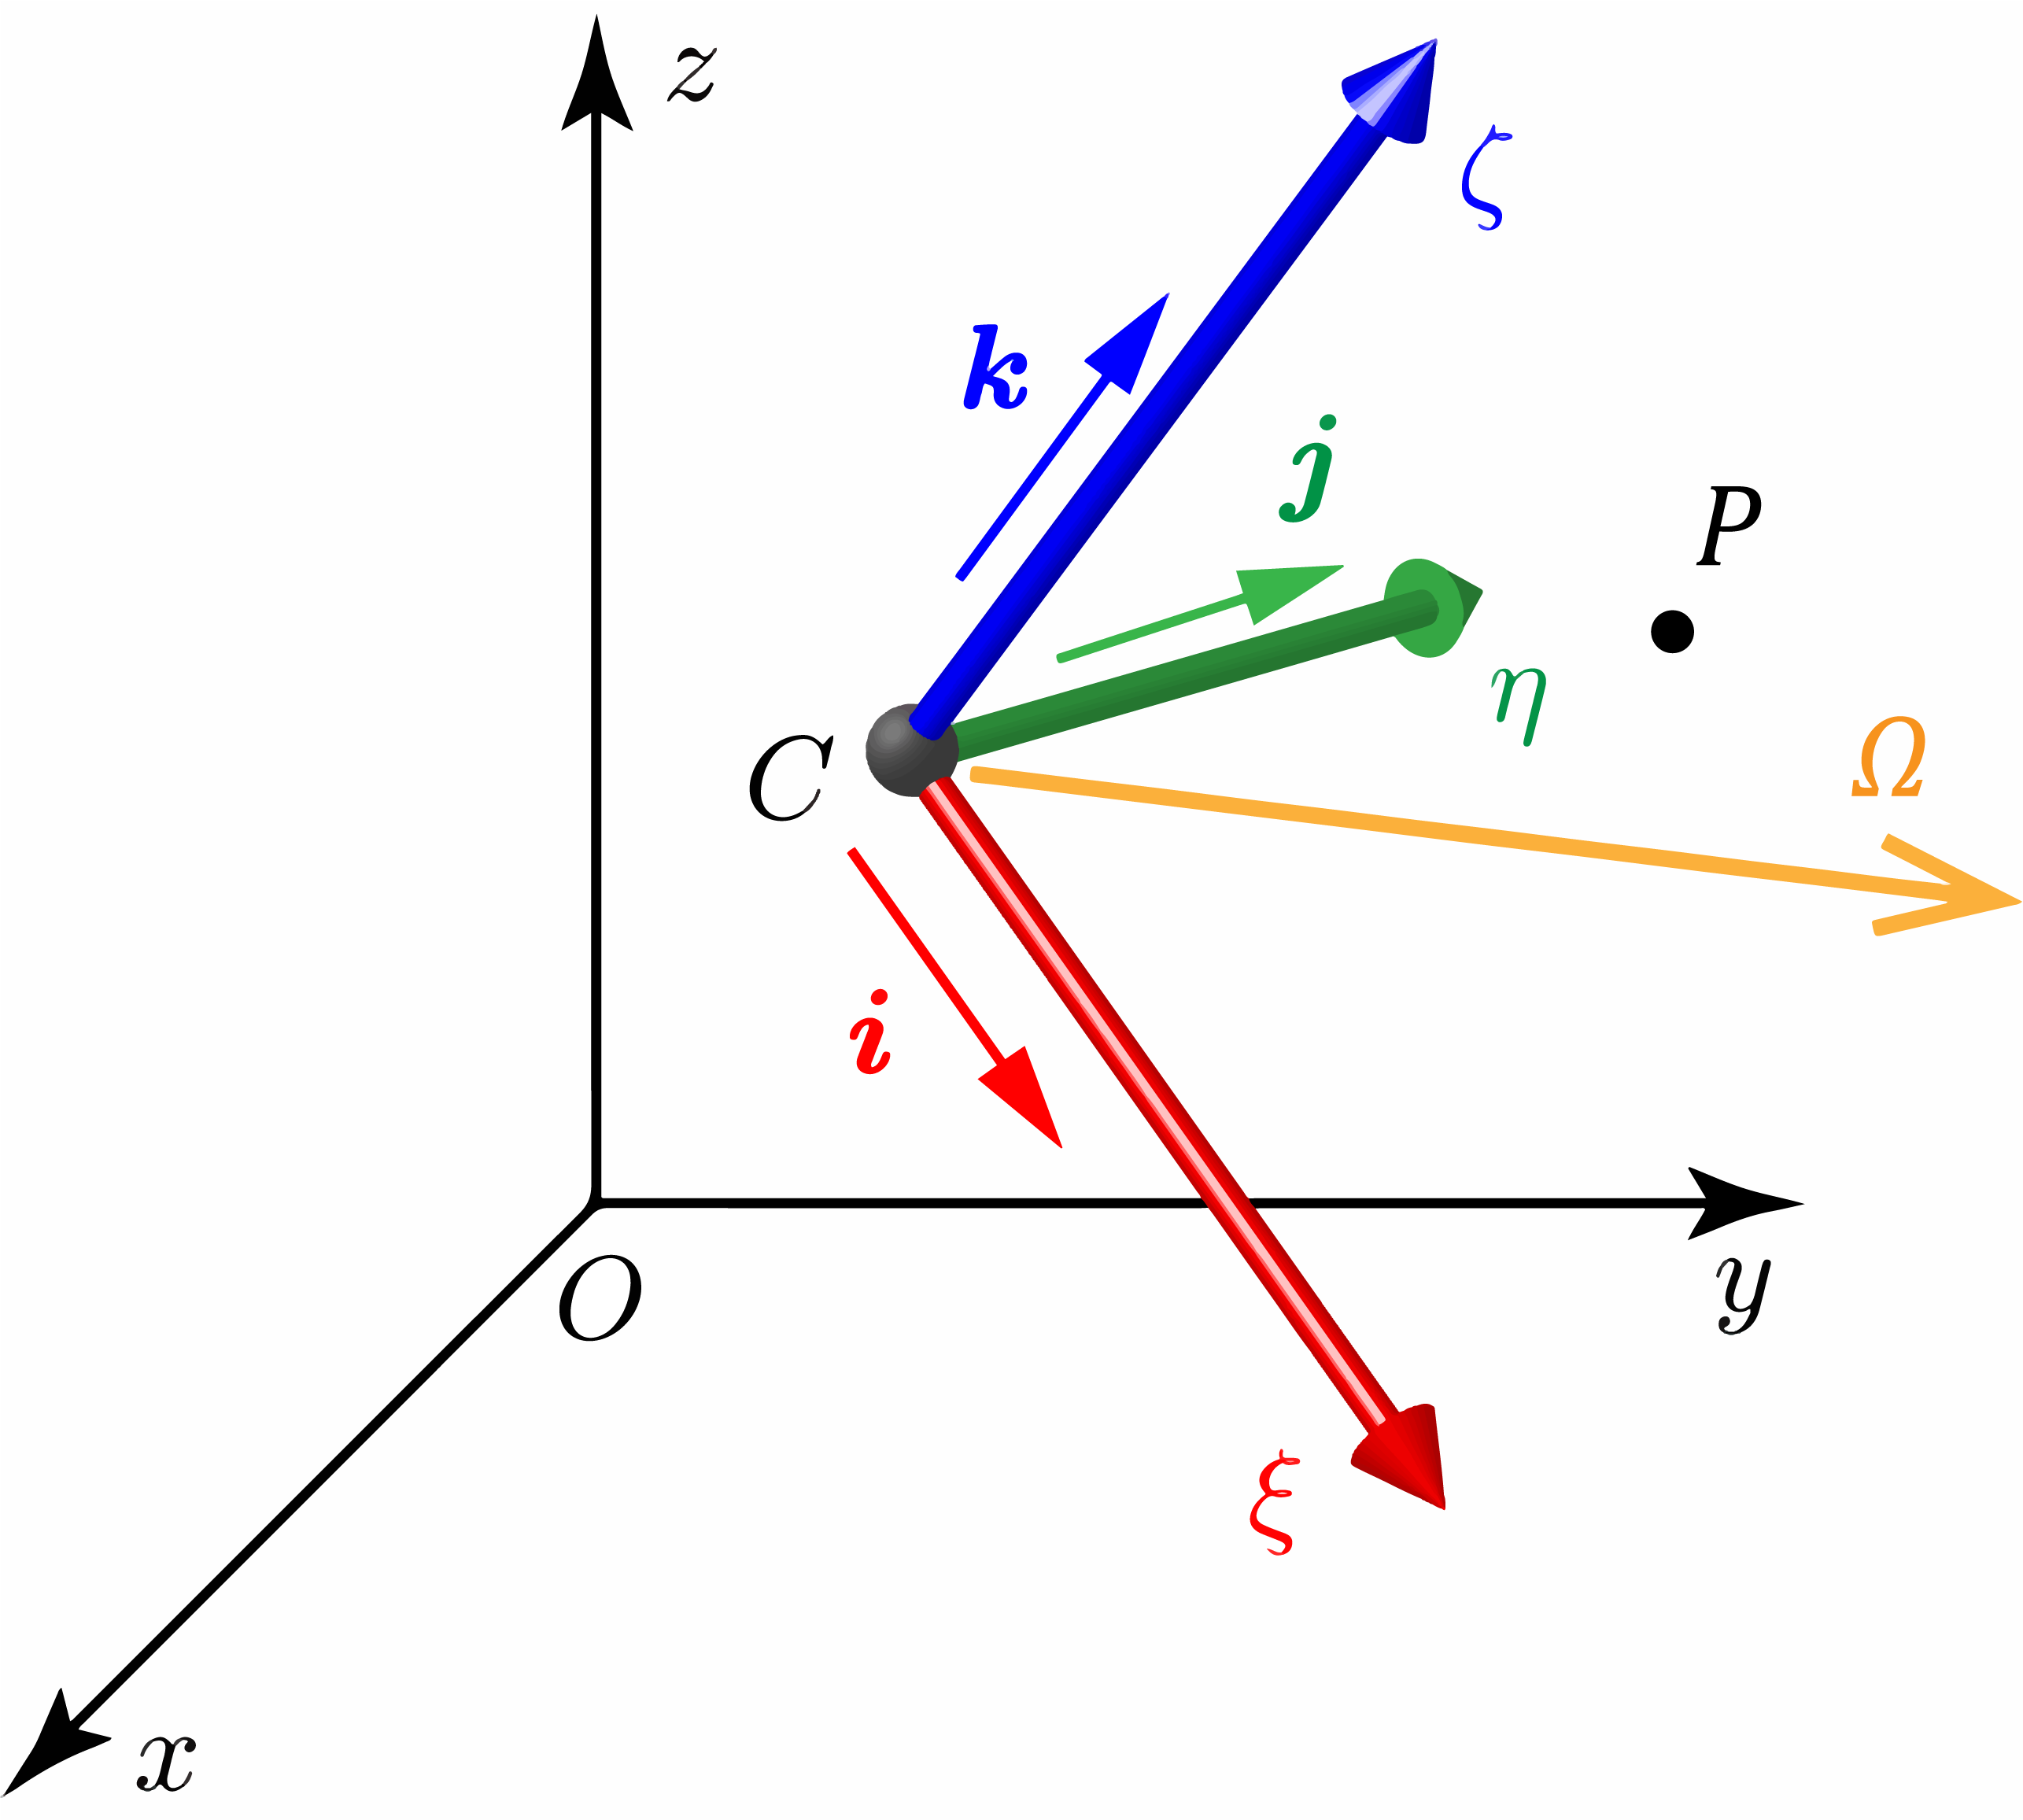
\includegraphics[width=6cm]{image/6-1-10.png}
\caption{参考系变换}
\end{wrapfigure}
第二点就是要给出新参考系的旋转角速度$\bs{\omega}$,\,角加速度记作$\bs{\beta}=\dot{\bs{\omega}}$.\,通过上一节我们知道,\,如果选取固连在新参考系的点$P$,\,并且把$\bs{CP}$记作$\bs{r}'$.\,那么$P$点速度加速度(现在记作$\bs{v}_c,\,\bs{a}_c$)为:
\[\bs{v}_c=\bs{v}_C+\bs{\omega}\times \bs{r}'\]
\[\bs{a}_c=\bs{a}_C+\bs{\omega}\times (\bs{\omega}\times\bs{r}')+\bs{\beta}\times\bs{r}'\]

我们现在研究什么问题呢?\,如果我们在$O-xyz$系中给出一个质点,\,也用$P$表示,\,的运动方程$x(t),\,y(t),\,z(t)$.\,其实也就给出了在$C-\xi\eta\zeta$系中的运动方程$\xi(t),\,\eta(t),\,\zeta(t)$.\,那么把位矢$\bs{OP}$记作$\bs{r}$,\,$\bs{CP}$记作$\bs{r}'$.\,再把$\bs{OC}$记作$\bs{r}_C$.\,于是得到恒等式:
\[\bs{r}=\bs{r}_C+\bs{r}'\]

但这不代表$\bs{v}=\bs{v}_C+\bs{v}'$.\,这里我们要注意有一点已经悄悄发生改变了,\,那就是导数,\,作为一个算符,\,变成了一个有多种自由定义余地的概念.\,只要想想这一点:\,从运动方程求出速度的过程叫做求导\footnote{导数就是从运动方程到速度矢量的映射},\,但是同一个运动方程对应的运动是同一个运动,\,但是在不同参考系中依然可以有多个不同的取值.\,这就足以说明有多种不同的求导方法.\,具体来说,\,这里的$\bs{r}'$可能有三种情况:\,a.\,固连在$C$系中,\,相对$C$系大小方向不变.\,b.\,相对地面系$O$系大小方向都不变,\,即$P$跟随$C$相对地面系平移.\,c.\,两者都不是.\,那么相应地定义三种导数:
\begin{enumerate}
	\item 绝对导数:\,即平常的$\displaystyle\frac{\ud}{\ud t}$,\,可以简单地用加点来代替.\,我们还创造一个新的符号$\uD$来表示求导,\,例如对于情形$b$,\,这个导数就是零.\,求导数的方法是:\,找到一个矢量在$O$系中每时每刻向三个坐标轴方向的投影分量并分别求导最后组合为矢量.\,用这个导数能定义$P$点在$O$系中的速度与加速度:
	\[\bs{v}=\uD \bs{r}(=\frac{\ud}{\ud t}\bs{r}=\dot{\bs{r}})\quad,\quad\bs{a}=\uD \bs{v} \]
	\item 相对导数:\,这就是要换相对$C$系的视角来研究一个矢量的导数了.\,我们记作$\uD'$.\,例如对于情形$a$,\,那么相对导数就是零.\,求导数的方法是:\,找到一个矢量在$C$系中每时每刻向三个坐标轴方向的投影分量并分别求导最后组合为矢量.\,这也就是说它用来定义相对速度和相对加速度是合适的:
	\[\bs{v}'=\uD'\bs{r}'=\dot{r_1'}\bs{i}+\dot{r_2'}\bs{j}+\dot{r_3'}\bs{k}\quad ,\quad \bs{a}'=\uD'\bs{v}'=\ddot{r_1'}\bs{i}+\ddot{r_2'}\bs{j}+\ddot{r_3'}\bs{k}\]
	\item 随体导数:\,这是矢量由于跟随$C$系转动而带来的相对$O$系的变化率.\,我们记作$\widetilde{\uD}$.\,例如在情形$a$中,\,$\bs{r}'$随体导数就是$\bs{\omega}\times\bs{r}'$.\,这个算符其实就等价于$\omega\times$,\,这是因为他就定义为:
	\[\widetilde{\uD}\bs{A}=A_1\bs{\ddot{\imath}}+A_2\bs{\ddot{\jmath}}+A_3\bs{\dot{k}}=A_1\bs{\omega}\times\bs{i}+A_2\bs{\omega}\times\bs{j
	}+A_3\bs{\omega}\times\bs{k}=\bs{\omega}\times(A_1\bs{i}+A_2\bs{j}+A_3\bs{k})=\bs{\omega}\times\bs{A}\]
\end{enumerate}

值得注意的是,\,这三个导数算符之间有如下关系:
\[\uD=\widetilde{\uD}+\uD'\]

这很容易证明,\,对一个矢量求导数,\,一看分量变不变,\,而看基矢量本身有没有旋转.\,那么就会产生两项.\,实际上就是莱布尼茨法则.

于是这才能推理参考系变换的公式.\,我们对$\bs{r}=\bs{r}_C+\bs{r}'$两边求绝对导数:
\[\bs{v}=\uD\bs{r}=\uD\bs{r}_C+\uD\bs{r}'=\bs{v}_C+(\widetilde{\uD}+\uD')\bs{r}'=\bs{v}_C+\bs{\omega}\times\bs{r}'+\bs{v}'\]

再次对上式两边求绝对导数:
\begin{align*}
\bs{a}=\uD\bs{v} &=\uD\bs{v}_C+\uD\bs{\omega}\times\bs{r}'+\bs{\omega}\times\uD\bs{r}'+\uD\bs{v}'\\
	  			 &=\bs{a}_C+\bs{\beta}\times\bs{r}'+\bs{\omega}\times(\widetilde{\uD}+\uD')\bs{r}'+(\widetilde{\uD}+\uD')\bs{v}'\\
	  			 &=\bs{a}_C+\bs{\beta}\times\bs{r}'+\bs{\omega}\times(\bs{\omega}\times\bs{r}')+\bs{\omega}\times\bs{v}'+\bs{\omega}\times\bs{v}'+\bs{a}'\\
	  			 &=\bs{a}_C+\bs{\beta}\times\bs{r}'+\bs{\omega}\times(\bs{\omega}\times\bs{r}')+2\bs{\omega}\times\bs{v}'+\bs{a}'
\end{align*}

这两个公式就是参考系变换下的变换公式:
\[\bs{v}=\bs{v}_C+\bs{\omega}\times\bs{r}'+\bs{v}'\]
\[\bs{a}=\bs{a}_C+\bs{\beta}\times\bs{r}'+\bs{\omega}\times(\bs{\omega}\times\bs{r}')+2\bs{\omega}\times\bs{v}'+\bs{a}'\]

如何理解以上的公式?\,事实上结构也很简单,\,我们把加速度中的最独特的一项单独拿出来叫做\emph{柯里奥利加速度}(Coriolis accelaration):
\[a_c'=2\bs{\omega}\times\bs{v}'\]

那么以上两公式具有以下结构:
\[\text{绝对}=\text{牵连}(+\text{柯氏})+\text{相对}\]

柯氏即柯里奥利.\,相对速度与相对加速度就是$\bs{v}',\,\bs{a}'$.\,言下之意就是我们定义了所谓的\emph{牵连速度}(convected velocity)与\emph{牵连加速度}(convected acceleration):
\[\bs{v}_c=\bs{v}_C+\bs{\omega}\times \bs{r}'\]
\[\bs{a}_c=\bs{a}_C+\bs{\omega}\times (\bs{\omega}\times\bs{r}')+\bs{\beta}\times\bs{r}'\]

细心的读者已经发现了,\,这两个式子和本节最开始推导出来的固连在$C$系中的点的绝对速度,\,加速度公式是一致的.\,牵连速度(加速度),\,顾名思义,\,被转动参考系``带着走''的速度(加速度).\,也正是以上规律启发我们总结出以下的动点动系法来理解看似复杂的速度加速度合成公式:
\begin{enumerate}
	\item 确定定系,\,动系,\,动点,\,定点.\,定系往往就是地面系;\,动系一般是相对某刚体或人为构造的刚性框架相对静止的参考系\footnote{注意,\,以下整个过程都可以脱离具体的坐标系而计算,\,这就为坐标系的选取(种类是直角坐标系,\,极座标系还是自然坐标系,\,方向如何)彻底提供了自由.};\,动点就是选做研究对象的相对两个系一般都有运动的点.\,最后,\,定点指的是这样的概念:\,在研究的一瞬间与动点重合,\,但是始终保持与动系固连的特殊参考点.
	\item 在定系考虑动点的运动.\,算出绝对量.\,在动系考虑动点的运动.\,算出相对量.\,在定系中考虑定点的运动,\,它的量就是牵连量.
	\item 建立绝对相对牵连之间的等量关系.
	\item 唯一要注意的是:\,只有当转动系是真转动的$\bs{\omega}\neq\bs{0}$,\,而且相对动系动点也是真运动的$\bs{v}'\neq\bs{0}$时,\,我们才有必要在加速度中添加一项柯氏加速度$2\bs{\omega}\times\bs{v}'$.\,从推导过程来看,\,一是即使固连在动系中的速度矢量也会跟随动系转动而带来加速度,\,二是动系中的相对位矢产生变化而带来在变化的牵连速度从而产生加速度,\,是造成柯氏加速度的两个因素.\,这一项不是因为在动系中的某特定位置而造成的,\,事实上与$\bs{r}'$无关,\,决定性因素是``相对动系有速度''.
\end{enumerate}

最后值得注意,\,如果$\bs{\omega}$和$\bs{\beta}$恒为零,\,这也并不少见,\,那么这样的动系就是\emph{平动系}(translational frame).\,此时公式极为简单,\,没有柯氏加速度,\,牵连量就是动系原点或任意固连点的量:
\[\bs{v}=\bs{v}_C+\bs{v}'\quad,\quad \bs{a}=\bs{a}_C+\bs{a}'\]

\subsection{刚体变换}

刚体的变换是点变换的直接推论.\,同样地,\,首先已知动系相对定系具有原点速度$\bs{v}_C$和加速度$\bs{a}_C$以及角速度$\bs{\omega}$和加速度$\bs{\beta}$,\,又已知定系中刚体基点速度加速度,\,现在记作$\bs{V},\,\bs{A}$.\,事实上我们还要给出刚体自己的角速度角加速度才算是对刚体的完整描述,\,它们为$\bs{\varOmega},\,\bs{B}$.\,那么绝对的和相对的各个量之间的关系为:
\[\bs{V}=\bs{v}_C+\bs{\omega}\times\bs{R}'+\bs{V}'\quad,\quad \bs{\varOmega}=\bs{\omega}+\bs{\varOmega}'\]
\[\bs{A}=\bs{a}_C+\bs{\beta}\times\bs{R}'+\bs{\omega}\times(\bs{\omega}\times\bs{R}')+2\bs{\omega}\times\bs{V}'+\bs{A}'\quad,\quad \bs{B}=\bs{\beta}+\omega\times\bs{\varOmega}'+\bs{B}'\]

证明过程留作练习由读者自己思考.

\section{运动的牵连}
最后本节旨在枚举一些在运动学解题中十分常见的初等模型与结论.

\subsection{接触系}
两个几何图形具有一个交点是一件非常常见的事情.\,交点将同时与两个几何图形保持结合关系.\,动态地看待这个问题,\,我们可以分别利用两个几何图形自身的运动和交点相对两者的运动合成来写出交点的速度矢量与加速度矢量来,\,但是作为同一个研究对象两种写法的结果理应相等.\,这构成了一组方程.

尤其是,\,在上述``相交系''中我们还有一类十分独特的情形,\,就是两个几何图形相切.\,两个平面形刚体如果始终保持相互接触,\,其轮廓之间就是这样的关系.\,此时要知道客观地这形除了一种约束:\,不是让两个刚体做任意运动都可以让两者保持相切的.\,所以必然存在所谓的\emph{约束方程}(equation of constraint).\,而这个方程的列法其实就是基于之前说的接触点的速度的一致性.

让我们看一个例子,\,它不仅帮助我们理解接触系,\,还可以帮助我们理解纯滚系.\,就是经典的在粗糙的地面上做匀速纯滚动的圆盘.\,首先应当注意到,\,涉及到所谓的``瞬时接触点''时可能指的是以下三个点之一:
\begin{wrapfigure}[8]{o}[-10pt]{7cm}
\vspace{0.1cm}
\centering
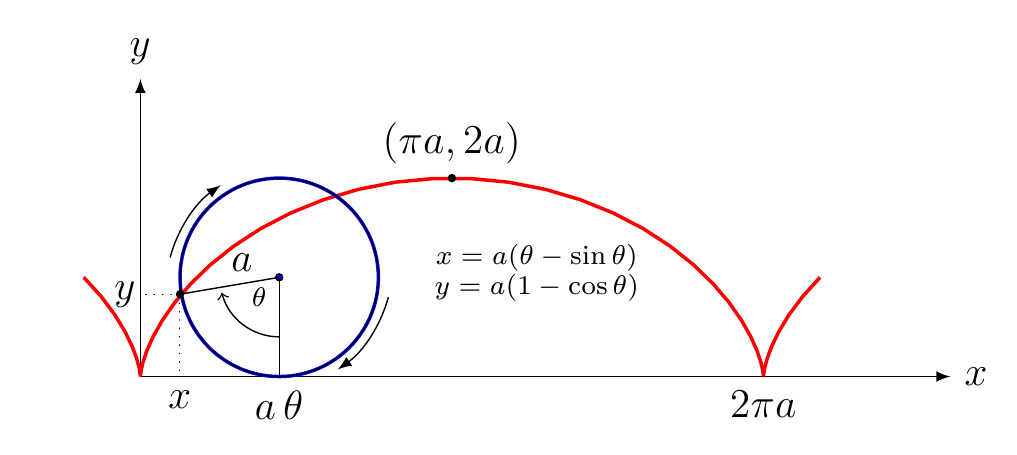
\includegraphics[width=7cm]{image/6-1-11.png}
\caption{圆盘在地面上做纯滚动}
\end{wrapfigure}

1.\,刚体1上的定点$P_1$.\,在这里取盘为刚体1,\,此时这个点是做旋轮线运动的那个点,\,此时恰好位于最低位置.

2.\,刚体2上的定点$P_2$.\,在这里取地面为刚体2,\,那么这个点就是一个静止的点.

3.\,动点$P_3$.\,就是每时每刻的切点形成的运动对象.\,在这里我们可以把圆盘变为圆筒,\,并且让一只松鼠在圆筒内部跑动以保持在最低位置,\,也就是每时每刻的切点.\,那么松鼠做匀速直线运动.

我们有什么结论呢?\,如果把$P_1$的瞬时速度在法线方向与切线方向的分速度与加速度写出来,\,分别是$v_{1n},\,v_{1\tau},\,a_{1n},\,a_{1\tau}$并约定法向以向刚体1内侧为正,\,切向可以以切线的任意一个方向为正.\,$P_2$同理为$v_{2n},\,v_{2\tau},\,a_{2n},\,a_{2\tau}$.\,那么让我们考虑一下$P_3$的速度与加速度.\,这就不难发现,\,如果采用动点动系法,\,就有:

速度:\,无论相对刚体1还是2,\,$P_3$的速度都是牵连加相对.\,牵连速度就是定点的速度,\,但相对速度由于点的轨迹就是刚体的轮廓,\,故方向必然在切线方向.\,然后由于速度的唯一性,\,这可以给出:
\[v_{1n}=-v_{2n}\]

加速度:\,道理是相同的,\,但需要注意两点,\,一是相对加速度具有了法线方向的分量.\,二是如果严格换一个刚体的转动系往往会带来柯氏加速度.\,具体解题时这仍然不失为一种常见的解题思路,\,但是难以总结现成的美妙,\,下一小节通过添加纯滚动这一更强的结论我们可以得到相应的方程.\,但是这个方程肯定是存在且可列式的,\,毕竟:

以上两个方程构成对接触系的约束的刻画.

\subsection{纯滚系}
上面的圆盘在地面上发生的运动实际上还是纯滚动.\,我们将首先给出纯滚动的定义,\,再来讨论纯滚动时的更强的附加条件,\,毕竟纯滚动相比简单的接触系还多一个约束.

事实上考虑相对运动就知道了,\,接触点在刚体1或2上相对运动的弧长就是相互滚动过的接触弧长,\,在两个刚体上应当具有公共值,\,这便是纯滚动的定义.\,这就是说:
\[\bs{v}_1'=\bs{v}_2'=\dot{s}\bs{\tau}\]

最后再利用$\bs{v}=\bs{v}_{1c}+\bs{v}_1'=\bs{v}_{2c}+\bs{v}_2'$.\,便得到了附加条件:
\[v_{1\tau}=v_{2\tau}\]

这就是常见的纯滚条件一,\,也就是说只有当相互接触的两个刚体定点切向速度一致才构成纯滚动.\,否则就是纯滚动的反面:\,必有相对滑动,\,俗称``连滚带滑''.

考虑加速度我们将得出一个不可思议但容易忽视的结论.\,首先注意到,\,如果两个刚体角速度分别为$\omega_1$和$\omega_2$,\,作为平面问题写成统一正方向的标量.\,而再设两刚体在接触点处轮廓的曲率为$k_1$和$k_2$.\,那么由于相对两刚体点在轮廓上的运动造成的单位时间切线方向的转角为:
\[\frac{\ud\theta_1}{\ud t}=\frac{\ud\theta_1}{\ud s}\frac{\ud s}{\ud t}=k_1\dot{s}\]
\[\frac{\ud\theta_2}{\ud t}=\frac{\ud\theta_2}{\ud s}\frac{\ud s}{\ud t}=k_2\dot{s}\]

而每当点成为切点两切线也会重合成为公切线,\,那么两个转角的和就是单位时间内两个刚体的相对转角:
\[\frac{\ud\theta_1}{\ud t}+\frac{\ud\theta_2}{\ud t}=|\omega_1-\omega_2|\]

最后,\,列出对刚体1和2牵连+柯氏+相对应当一致的方程:
\[a_{1n}-2\omega_1 \dot{s}+k_1\dot{s}^2=-(a_{2n}-2\omega_2\dot{s}+k_2\dot{s}^2)\]

整理得到纯滚条件二:
\[a_{1n}+a_{2n}=\frac{(\omega_1-\omega_2)^2}{k_1+k_2}\]

这是一个必然大于零的表达式\footnote{注意$k$本身可以小于零,\,但两个$k$的和必然大于零.},\,它意在,\,两个相接触的点必然后来会分离,\,这个分离加速度只与两刚体瞬时转动快慢和接触点弯曲程度有关,\,与平动转动加速度都没有关系.

\subsection{约束系}
约束是一种普遍存在且可以普遍讨论而有很广的适用范围的物理现象.\,本节并非要详细讨论约束,\,这一点在之后第三章静力学中再加以详细讨论.\,这里只讨论两个问题:\,绳系和杆系.

对于不可伸长的轻绳模型,\,如果它也被拉直(因为内部受力不为零又没有外力).\,那么在运动学层面上就等价于不可伸长的轻杆.\,设杆长为$l$,\,把两端点1和2速度加速度沿平行与杆与垂直与杆方向分解,\,具有关系:
\[v_{1\perp}-v_{2\perp}=\omega l\]
\[v_{1\parallel}-v_{2\parallel}=0\]
\[a_{1\perp}-a_{2\perp}=\beta l\]
\[a_{1\parallel}-a_{2\parallel}=-\omega^2 l\]

其中第二个关系就是著名的端点沿杆方向分速度必须是常数.\,对于绳子,\,即使绕过了定滑轮,\,显然沿定滑轮的切向速度也一直不变,\,因为绳子不可伸长.

最后,\,如果绳子允许弯曲但不允许伸长,\,其运动学约束方程该如何列?\,那就要求绳子上每一点在``局部''沿切向方向没有相对速度,\,表示为公式就是:
\[\frac{\ud \bs{v}}{\ud s}\cdot\bs{\tau}=0\]

注意这个条件不可以写为:
\[\frac{\ud v_\tau}{\ud s}=\frac{\ud (\bs{v}\cdot\bs{\tau})}{\ud s}=0\]

% %!TEX root = ../physical-olympics-2.tex
\chapter{动力学}


\section{牛顿定律}

\subsection{概述}
中世纪到近代以来物理学的发展,\,可谓沧海桑田,\,旧的观点被否定,\,几十年以后突然又以全新的面貌出现在物理学理论中.\,其中,\,实验中观察到各种令人惊诧的结果,\,无论物理学所依托的数学形式一变再变,\,要说亘古不变的主题,\,恐怕只有自然界的神奇与深邃,\,和我等凡人难以参透其中奥妙却仍为之孜孜不倦研究的决心.\,物理是一门研究自然界存在的运动并提出解释与理解方法的学科.\,运动形式多种多样,\,变化万千,\,但很多都被我们或多或少地解释,\,其实总结来看,\,从古至今我们也仅仅拥有过两类解释:\,一类由牛顿提出,\,一类则来自爱因斯坦.\,前前后后经历了大概以下发展:

\begin{description}
	\item[亚里士多德:]\, 天体运行,\,自由落体是自然(nature)的运动;\, ``树欲静而风不止''是强迫(violent)的运动.\,但错误地认为``物体越重,\,下落越快''
	\item[伽利略:]\, 辩证地看待亚里士多德的观点,\,开创性地提出相对性原理,\,成功论证与形成惯性与常见运动的正确认识.
	\item[笛卡尔,\,惠更斯等:]\, 成功得到大量动力学公式,\,包括后来的牛顿第二定律,\,动能的表达式与能量守恒定律,
	\item[牛顿开创的相互作用观:] \, 开创性的提出物质间存在相互作用,\,相互作用是改变物质运动状态的原因.\,并很好地把天体的运动归结到互相之间产生的相互作用上.\,后人建立了场的理论以后,\,超距的粒子间相互作用就不再被理论学家们采纳了,\,而要理解为场与粒子的相互作用,\,再晚一点,\,场和粒子都被赋予了波粒二象性,\,粒子也要被理解为场,\,但所有场都要被被分解为平面波,\,平面波又要被量子化.\,如果没有相互作用,\,那么这些平面波的运动状态就不会发生改变,\,只有相互作用才会改变其运动,\,或传播方向发生偏折(发生散射),\,或强度发生改变(粒子的产生与湮灭).\,牛顿的观点是以\emph{相互作用}(interaction)为核心的观点.
	\item[拉格朗日,\,哈密顿等:]\, 将牛顿的结果与观点上升到\emph{分析力学}(analytic mechanics)的高度.\,将复杂体系的结构浓缩在统一的一个能量函数或作用量泛函数中.\,为后来场论建立和相对论,\,统计力学,\,量子力学的发展都提供了理论支持.
	\item[马赫:]\, 批判牛顿的过于绝对的时空观.\,预言质量分布会对惯性本身产生影响.
	\item[爱因斯坦开创的几何观:] \,  仿佛又回到了亚里士多德,\,不仅仅是无相互作用下的匀速直线运动,\,一切在万有引力下的天体运动其实也是``自然''的运动.\,看上去复杂的曲线运动不过也是沿对被引力所扭曲的弯曲时空几何下的天然``直线''---测地线(geodesic)运动而已.\,对引力问题提出开创性的解释.\,率先描绘了20世纪建立的若干理论的物理图像.
	\item[天体物理,\,粒子物理:]\, 爱因斯坦以后的理论研究中很多问题还处于开放状态.\,时而采用牛顿的相互作用观,\,时而采用爱因斯坦的几何观.\,是一种两个图像的有机结合.
\end{description}

我们今天说\emph{经典力学}(classical mechanics)大多数情况即指\emph{牛顿力学}(Newtonian mechanics),\,指的是由伽利略最初引领,\,笛卡尔,\,惠更斯等奠基,\,牛顿集大成的一套理论.\,它以伽利略的\emph{两种新科学的对话与数学展示}(Discorsi e dimostrazioni matematiche intorno a due nuove scienze)和牛顿的\emph{自然哲学的数学原理}(Philosophi\ae\ Naturalis Principia Mathematica)两篇文献为核心.\,逻辑上以质点的牛顿三大定律为基础.\,不包括后来上升到的分析力学层次,\,作为绝对时空观适用伽利略变换,\,不兼容相对论.

牛顿定律总结如下:
\vspace{0.5cm}

\hrule
\begin{enumerate}
	\item 第一定律:\quad 在惯性系中,\,一个质点应静止或匀速直线运动.\,除非有外力施加于物体.
	\item 第二定律:\quad 在惯性系中,\,质点受力的矢量和$\bs{F}$等于其质量$m$与加速度$\bs{a}$的乘积.
	\item 第三定律:\quad 一个质点对另一个质点施加作用力时,\,另一个质点同时将施加反作用力于第一个质点,\,作用力与反作用力等大反向共线.
\end{enumerate}
\hrule
\vspace{0.5cm}

三个定律之间的联系是很值得讨论的.\,对三个基本定律的设置反映了很多物理思想\footnote{例如爱因斯坦狭义相对论的两个假设在某种意义上与牛顿第一第二定律的逻辑完全一致.\,都是先定义时空背景再阐述物理规律的共性.}.\,分析如下:

\subsection{牛顿第一定律}
牛顿第一定律旨在阐述时空的平直性.

也正基于以上这一点,\,我们不能仍为牛顿第一定律可以由牛顿第二定律出发推导.\,它不是表面上的牛顿第二定律中$\bs{F}=\bs{0},\,\bs{a}=\bs{0}$的特例.\,恰恰相反,\,即使从形式上看,\,也应当先由牛顿第一定律给出\emph{惯性系}(inertial frame)的概念才能适用牛顿第二定律.\,那么怎样的参考系是惯性系呢?\,牛顿第一定律是暗含认可\emph{绝对惯性系}(absolute inertial frame)的存在性的.\,在这样第一个系中牛顿第一定律才可以成立.\,这一个系无非就是由某种特殊运动状态的观察者(绝对观察者)建立的三维欧几里得空间坐标系外带一维时间坐标.\,而只要质点不受力(力是对相互作用的描述,\,只要远离其它所有物质就会使质点成为\emph{孤立}(isolated)的),\,就会静止或匀速直线运动,\,所谓匀速直线运动是指:
\[\begin{pmatrix}x(t)\\y(t)\\z(t)\end{pmatrix}=\begin{pmatrix}x(0)\\y(0)\\z(0)\end{pmatrix}+\begin{pmatrix}v_x\\v_y\\v_z\end{pmatrix}\cdot t\]

其中三个速度$v_x,\,v_y,\,v_z$都是常数.\,但是我们发现,\,相对这个系做匀速直线运动的另一个无自转观察者建立的系中,\,原来做匀速直线运动的质点现在依然做匀速直线运动.\,所以这样的系也叫做惯性系,\,可以叫做相对惯性系.\,即:\,惯性系就是任何相对绝对惯性系做匀速直线平动的参考系.\,而惯性系就是牛顿定律成立的前提条件.

所以牛顿的经典力学体系的第一大特点是承认绝对惯性系的存在性.\,实际上承认这一点也几乎等价于承认了时空的平直性.\,只不过在众多彼此等价(任何物理实验都不足以判断这些系的不等价性)的系中,\,牛顿认为还应当有一个第一性的,\,``最初''的惯性系.

\subsection{牛顿第二定律}
牛顿第二定律是牛顿定律的核心,\,旨在描述相互作用对运动的影响.

\emph{相互作用}(interaction)是牛顿经典力学后经过了几百年发展而浓缩出来的更普遍的概念.\,如果没有相互作用,\,物质基本的运动模式就是``惯性''的,\,如匀速运动的粒子或传播的平面波.\,任何使物质偏离这种``惯性''运动的模式的原因就都在相互作用上.\,相互作用的模式是多种多样的,\,除了牛顿指出的下面仔细讨论的情形,\,光会因为与物质相互作用而产生吸收和散射,\,两个惰性气体原子靠近时两个电子云也会产生量子的诱导极化而使原子间产生范德瓦耳斯吸引.\,这些都是广义的相互作用,\,但是为了描述它们,\,前者需要借助波来描述光这种物质,\,后者还需要借助波函数来描述电子云,\,相互作用更是要依赖于薛定谔方程等来理解.\,所以经典物理理论有它的适用性,\,这一点在下面我们需要记住.

这也就是牛顿经典力学体系的第二大特点了:\,物质的基本模型一律视作\emph{质点}(mass point)\footnote{牛顿甚至认为光也适用于质点模型},\,相互作用的基本模型一律视作\emph{力}(force),\,质点具有惯性这一基本属性,\,用\emph{质量}(mass)来描述.

从牛顿第二定律$F=ma$形式上看,\,难免会由于数学思维得出``用力来定义质量的多少''或者是``用质量定义力的大小''这样的观点,\,而进入力与质量循环定义的误区.\,但实际上谁也没有定义谁.\,因为正常的物理思维是先要提前定义质量和力:

首先质量是受力物体所固有的属性之一,\,它具有广延性:\,如果把质量为$m_1$的质点与质量为$m_2$的质点复合为一个大质点,\,其质量变为$m_1+m_2$.\,可比性:\,任意两个质点的质量都可以依照在同样大小的力下的行为来比较其质量的比例关系\footnote{事实上用碰撞实验可以给出一个更简单的比较质量的方法,\,让待测质量的质点以一个单位的速度去正碰撞一个以$x$个单位速度运动的单位质量的质点,\,若恰好停下就说明待测质量为$x$个单位质量,\,若没停下就改变$x$的值直到停下.}.\,和固有性:\,只要质点没有变性,\,质量就不变,\,所以在不同参考系去看同一个质点,\,在运动的不同时刻质量都是严格不变的,\,也称``质量守恒'',\,我们将避免这一称呼,\,因为一般的守恒量只是针对一个参考系中的过程中的各个状态,\,而换一个系看守恒量往往要变,\,质量却显然不变,\,这是其一;\,另外相对论下质量就不再守恒了,\,它不普遍,\,这是其二.

力也是对固有的相互作用的强度做的描述.\,它也是固有的,\,应当有一种合理的公式去描述施力物体的状态如何影响施加的力(这个力也与受力物体的状态有关).\,而且如果换一个参考系考虑,\,力的强度是不变的.\,根据力对质点产生的效果,\,力也应当具有矢量性,\,不同两个力是可以比较的,\,很多情况下甚至可以叠加:\,多个施力物体互不影响各自施加的力,\,同时作用于同一个受力物体,\,在生活中这种现象非常常见,\,不难得出这样的总结.

于是才有了牛顿的著名论断:
\[\bs{F}=m\bs{a}\]

这样一个定律内容是丰富的,\,它首先是兼容于伽利略相对性原理从而自洽:\,在另外的惯性系中考察,\,$F$和$a$都是不变的.\,但是又不是兼容于相对性原理的唯一解决方案,\,狭义相对论,\,就提供了另一套可能性,\,在低速极限$v\ll c$时狭义相对论的动力学方程表达式和这并无二致;\,其次质量$m$作为系数联系了力(原因)与加速度(结果)这并不是偶然,\,它也是为了和叠加原理相协调:\,一份的力作用在一份质点上产生这样的加速度,\,那么把两份力各自作用在两份质点上那就还是产生同样的加速度.\,所以力除以质量决定运动学加速度\footnote{即$F/m=f(v,\,a)$}那是天经地义.\,至于为什么两份力作用在原来的一份质点上会产生加速度加倍的效果,\,这就是经典力学中的类似于公理性质的存在了.

\subsection{牛顿第三定律}
牛顿第三定律是对``相互作用''中的``相互性''的刻画,\,暗示了动量与角动量守恒.

任何物理理论,\,如果妄想在短短几条式子中道尽万千世界发展与变化的规律,\,都是玄学而不是科学.\,科学的精神是要基于事实,\,进行总结与归纳,\,借助数学进行基本的抽象与再创造.\,所以现实就是,\,世界的运行本就是复杂的,\,不可预测的.\,物理学的发展史也就充满了惊人的转折:\,每当人们以为在某一个大的领域有简单而清晰的图像共识的时候,\,总是会有意外发生告诉人们特殊情况下理论不再适用.\,原则上,\,没有任何命题能够成为物理学上的公理:\,它能无条件适用于从宇观到微观的方方面面.

牛顿清楚地意识到了物质与物质之间相互作用的复杂性,\,是不可能用几个简单的公式写出所有情况下他的理论中两个任意质点之间的作用力的.\,所以退而求其次,\,用牛顿第三定律来描述了所有情形下这样的力需要满足的条件.\,的确合情合理.\,但是又看牛顿第三定律的提法本身是否合理?

实际上我们先注意到动量守恒和角动量守恒的条件比牛顿第三定律的条件要强(也更本质):\,我们可以由前者推导出后者.\,以动量为例,\,动量是用来描述一个体系的动力学运动趋势的.\,动量守恒就意味着,\,如果一个孤立的体系的一部分``平均地''在初始时刻具有向前运动的趋势,\,比如一部分向前运动而另一部分静止.\,那么之后就绝对不可能演化为向后运动.\,或者还可以这么理解:\,如果看到一个质点在做一个非匀速直线运动:\,比如忽快忽慢的直线运动,\,那么显然单独看质点本身动量并不守恒.\,但是这必然意味着质点不是孤立的,\,必须和别的体系一同看作一个整体,\,质点增加或减少的动量必须由体系的另一部分的动量减少或增加来抵消,\,来满足整体动量守恒的需求.\,如果体系仅仅由两个质点构成,\,再把动量的增加或减少的快慢理解为受力(动量定理),\,我们就有了牛顿第三定律中关于相互作用力等大,\,反向的部分.

所以动量守恒可以用来``证明''牛顿第三定律中的一对相互作用力.\,同理角动量守恒则可以用来证明牛顿第三定律中质点间相互作用力共线的部分.\,最后读者可以验证牛顿第三定律的数学形式为\footnote{$\bs{F}_{12}$表示1给2的力.}:
\[\bs{F}_{12}+\bs{F}_{21}=\bs{0}\quad,\quad \bs{r}_2\times\bs{F}_{12}+\bs{r}_1\times\bs{F}_{21}=\bs{0}\]

之所以这么理解是因为,\,动量守恒和角动量守恒显得更普适.\,事实上,\,它们是体系物理规律在空间平移对称性和旋转对称性下具有协变形式的直接推论.\,这一点是由近代著名的\emph{诺尔特定理}(Noether Theorem)这一数学定理精确证明了的.

也正是牛顿第三定律暗示了牛顿经典力学体系的缺点.\,因为我们无法解释牛顿第三定律的``自然性'',\,取消牛顿第三定律所构成的体系无非是具有外力的非孤立系(动量不守恒),\,牛顿第三定律为体系增添的``结构性要求''并没有很好地由理论解释与包含.\,所以才有了后来建立在对守恒量,\,尤其是能量进行强调的分析力学理论的提出.

\subsection{质点系与它的牛顿定律}
对于复杂体系,\,牛顿提出一种可能的等效观点,\,就是把任意这样的体系看做是一种离散的质点系的推广.\,质点系由质点集合$\{(m_i,\,\bs{r}_i)\},\,(i=1,\,2\,\cdots \,n)$组成.\,我们只要找到从质点理论到有限质点构成的质点系理论中那些不变的结论,\,就有理由相信这些结论可以推广到复杂的真实体系.\,因为真实体系被期待可以用一个足够大数目的质点系来近似.\,对于复杂的质点系首先需要引入\emph{质心}(center of mass,\,{\rm CM})的概念:
\[\overline{\{(m_i,\,\bs{r}_i)\}}=(m_C,\,\bs{r}_C)\]

我们的做法是:\,直接把质心理解为一个新的质点,\,它具有新的质量$m_C$和位置$\bs{r}_C$,\,并满足表达式:
\[m_C=\sum_i m_i\quad;\quad \bs{r}_C=\frac{\sum_i m_i\bs{r}_i}{\sum_i m_i}\]

可以把上式读作:\,质心的质量等于质点系的总质量,\,质心的位矢是各个质点位矢关于质量的加权平均.

质心的求法是符合交换律与结合律的.\,这在质量上是显然的,\,因为质心质量就是各个质点质量构成的连加式.\,对于质心位矢,\,考虑总质量为$m_1$的第一个质点系$(m_{1i},\,\bs{r}_{1i})$和总质量为$m_2$的第二个质点系$(m_{2j},\,\bs{r}_{2j})$复合而成的整个质点系,\,如果直接算两个体系质心形成的质心:
\[\frac{m_1\bs{r}_{1C}+m_2\bs{r}_{2C}}{m_1+m_2}=\frac{\displaystyle\sum_i m_{1i}\cdot \frac{\displaystyle\sum_{i} m_{1i}\bs{r}_{1i}}{\displaystyle\sum_i m_{1i}}+\displaystyle\sum_j m_{2j}\cdot\frac{\displaystyle\sum_{j} m_{2j}\bs{r}_{2j}}{\displaystyle\sum_{j} m_{2j}}}{\displaystyle\sum_i m_{1i}+\displaystyle\sum_j m_{2j}}=\frac{\displaystyle\sum_{k\in 1\& 2}m_k\bs{r}_k}{\displaystyle\sum_{k\in 1\& 2}m_k}\]

可以发现这就是整个体系的质心.\,这种方法就是``组合法'',\,比如求几根棍子的质心,\,可以把棍子替换为在质心的质点再求.\,由此还可以引申出``割补法''或者``负质量法'',\,不过就是把上式反过来理解:\,如果我们要求第一个体系的质心,\,不难验证可以这样求:
\[\bs{r}_{1C}=\frac{m\bs{r}_C-m_2\bs{r}_{2C}}{m-m_2}\]

动态地看待求质心的式子,\,还可以发现,\,求导以后,\,我们得到了质心作为一个在运动的质点,\,其速度,\,加速度也是可以直接从原质点系来做加权平均的:
\[\bs{v}_C=\frac{\sum_i m_i\bs{v}_i}{\sum_i m_i}\quad;\quad \bs{a}_C=\frac{\sum_i m_i\bs{a}_i}{\sum_i m_i}\]

为了推导出质点系的类似的牛顿定律,\,我们发现牛顿三大定律是缺一不可的.\,当然原则上如果没有牛顿第三定律,\,我们就把作用在每一个质点$m_i$上的合力,\,不管施力物体是谁,\,记作$\phantom{}^tF_i$,\,``t'' for ``total''.\,原则上我们也可以得到:
\[\phantom{}^t\bs{F}=\sum_i m_i\bs{a}_i\quad \phantom{}^t\bs{F}=\sum_i\phantom{}^t\bs{F}_i\]

这一点很容易证明,\,只需要把每个质点的牛顿定律加起来即可.\,但是注意到牛顿第三定律既然正确,\,我们就可以做进一步的研究:\,把任何质点受力分解为\emph{内力}(internal force)和\emph{外力}(external force):
\[\phantom{}^t\bs{F}_i=\phantom{}^{in}\bs{F}_i+\phantom{}^{ex}\bs{F}_i\]

内力指$i=1,\,2\,\cdots\,n$个质点之间一对一对存在的力,\,所以实际上不如写明:
\[\phantom{}^{in}\bs{F}_i=\sum_{j\neq i}\bs{F}_{ji}\]

最后单独的那个真正的外力以后直接简写为$\phantom{}^{ex}\bs{F}_i=\bs{F}_i$.

经过这么一番折腾完以后,\,我们还是把所有质点的牛顿定律来求和,\,但是注意到由于牛顿第三定律关于相互作用力等大反向的部分,\,内力相互抵消,\,得到:
\[\bs{F}=\sum_i m_i\bs{a}_i\quad \bs{F}=\sum_i \bs{F}_i\]

这就是质点系的牛顿第二定律,\,相比上面那个也对的直接把每个牛二加起来的表达式,\,能引起注意的变化只有一点,\,那就是:\,不需要考虑内力!\,但正是这一点极大地简化了很多实际问题的分析.

值得一提,\,我们顺理成章地要考虑另外两个层面的规律,\,一是``对质心'',\,二是``相对质心''.\,前者值的是,\,把质心作为一个质点来研究问题.\,那么问题也很简单,\,利用之前证明过的:
\[\bs{a}_C=\frac{\sum_i m_i\bs{a}_i}{\sum_i m_i}\quad \Rightarrow \quad m_C\bs{a}_C=\sum_i m_i\bs{a}_i\]

就可以得到:
\[\bs{F}=m_C\bs{a}_C\]

这就是著名的\emph{质心运动定律}(motion law of {\rm CM}).\,特殊的,\,如果合外力$\bs{F}=\bs{0}$.\,那么退化到\emph{质心守恒}:\,质心做匀速直线运动或者静止.

最后我们提出质心系的概念.\,\emph{质心系}(frame relative to {\rm CM})指:\,原点在质心的平动欧几里得坐标系.\,结合我们已经学过的和将来要学的所有内容我们把其性质罗列如下,\,请读者能够给出证明的直接证明,\,给不出的带着问题往下学习:
\begin{itemize}
	\item 质心系虽然有非惯性力,\,但非惯性力与原力系主矢和为零.
	\item 质心系虽然有非惯性力,\,但非惯性力系对质心的主矩为零.
	\item 质心系是零动量系.
	\item 质心系虽然有非惯性力,\,但非惯性力在过程中总功和为零.
	\item 取质心为原点能使质点系二阶矩最小,\,故刚体相对所有平行轴中以过质心的轴转动惯量最小.
	\item 只有取质心才能写出柯尼希定理.
\end{itemize}

\subsection{非惯性系的处理}
虽然牛顿定律只在惯性系中成立.\,但是如果我们选取一个相对惯性系的转动系,\,其原点速度加速度为$\bs{v}_C$与$\bs{a}_C$.\,而角速度与角加速度分别为$\bs{\omega}$与$\bs{\beta}$.\,本来在原来的惯性系中研究一个质点,\,正确的式子是:
\[\bs{F}=m\bs{a}\]

现在换了参考系以后,\,将不能仿照上式写出一个依然正确的式子.\,但是加速度变换总是对的:
\[\bs{a}=\bs{a}_C+\bs{\beta}\times\bs{r}'+\bs{\omega}\times(\bs{\omega}\times\bs{r}')+2\bs{\omega}\times\bs{v}'+\bs{a}'\]

而我们也永远认为力矢量在参考系变化下是大小与方向都不变的:
\[\bs{F}=\bs{F}'\]

代入就足以得到依然正确的,\,仅仅用新的非惯性系中的各个参量表示的类牛顿定律.\,我们以后将直接叫做非惯性系中的牛顿定律:
\[\bs{F}'+(-m\bs{a}_C)+(-m\bs{\beta}\times\bs{r}')+[-m\bs{\omega}\times(\bs{\omega}\times\bs{r}')]+(-2m\bs{\omega}\times\bs{v}')=m\bs{a}'\]

可以发现,\,这类似于需要为质点运动虚构一些力,\,它们全都称作\emph{惯性力}(force of inertial).\,包括:
\begin{itemize}
	\item 平动惯性力$-m\bs{a}_C$,\,典型的情况就是平动而非转动的非惯性系中的惯性力.\,特点是一个恒力,\,而与质点的运动状态无关.
	\item 切向惯性力$-m\bs{\beta}\times\bs{r}'$与惯性离心力$-m\bs{\omega}\times(\bs{\omega}\times\bs{r}')$,\,典型的情况是绕轴做旋转的参考系.\,特点是这两个力仅仅依赖于质点的位置,\,离轴越远力越大,\,在轴上力就消失了.
	\item 柯里奥利力$-2m\bs{\omega}\times\bs{v}'$,\,典型的情况是相对转动系还有运动的情况.\,特点是给出一个与位置无关,\,但是正比与速度大小,\,方向始终垂直于速度方向的力.
\end{itemize}

如果我们的研究对象是一个刚体而非质点,\,那么相当于每一个质点上都要受到不同的惯性力.\,此时如果考虑这些所有力作用在刚体上的等效合力和力矩,\,那么将是一个非常复杂的情况,\,尤其是,\,各个柯里奥利力将对刚体整体造成所谓的``回转力矩'',\,用这个观点可以解释很多第七章刚体中的现象,\,感兴趣的读者可以参考相关资料.

\section{动量定律}
这四节我们将罗列质点与质点系动力学的核心内容.\,读者应当具有初等的牛顿理论的基础.\,这一部分与三个牛顿定律的关系如何?\,首先它们是牛顿定律的自然延伸,\,属于并占据经典力学的主要部分.\,其次这些结论与相关推论适用性很强.\,比如三个守恒律:\,动量能量与角动量的守恒几乎是在所有物理理论中普适的.\,从内容上看关于质点系的定律自然就包含了单质点的相应特殊情况.\,而写法总是有三种:\,相对地面系的,\,相对质心系的和把质心作为质点的.\,联系三种写法的是质心系独有的各个柯尼希定理.\,最后,\,能量比较特殊我们单独列一小节多加阐述,\,具体的碰撞问题加一节,\,最后再补充一个新的位力定律.\,便构成了一$3\times3$条定律为主干的本章的内容.\,实际上也就是牛顿经典力学的核心部分.

\subsection{质点的动量}
质点的\emph{动量}(momentum)定义为:
\[\bs{p}=m\bs{v}\]

很直接地可以推导出质点的\emph{动量定理}(law of momentum)来,\,用$\bs{F}$表示合力:
\[\bs{F}=\frac{\ud \bs{p}}{\ud t}\]

证明过程就是把牛顿定律右侧拿来等量代换.

质点动量守恒并不是守恒律最常见的提法.\,但是不管怎样,\,我们能看出来,\,如果在某方向\footnote{必须是直角坐标!\,比如极坐标下$F_\theta=0$但$p_\theta$不守恒,\,$L=rp_\theta$才是对应的守恒量,\,个中缘由涉及到分析力学.}分力为零,\,那么该方向分动量导数为零,\,从而是一个不变量.

\subsection{质点系的动量}
依据上一节的符号约定,\,质点系$\{m_i,\,\bs{r}_i\}$中第$i$个质点的牛顿定律写作:
\[\bs{F}_i+\sum_{j\neq i}\bs{F}_{ji}=m_i\bs{a}_i\]

所谓质点系的动量定理,\,无非就是把上式拿去对每一个质点求和,\,然后等号右侧化为动量的形式.\,过程中我们发现需要定义:

质点系的总动量:
\[\bs{p}=\sum_i \bs{p}_i=\sum_i m_i\bs{v}_i\]

外力矢量和:
\[\bs{F}=\sum_i \bs{F}_i\]

过程中内力全然抵消,\,这就导致了最后表达式简单地为:
\[\bs{F}=\frac{\ud \bs{p}}{\ud t}\]

\vspace{0.5cm}

接下来就是研究质心的两个层次,\,一是把质心作为质点研究等号左侧的``作用''和等号右侧的``动力学量'';\,二是考虑相对质心系的引入惯性力以后的新写法.

如果在地面系中质点系受到一个力$\bs{F}_\alpha$,\,那么把这个力移动到质心上以后,\,我们认为这个力是不需要改变的.\,但是如果考虑相对质心系,\,固然原来的力也是存在且不变,\,但是还得考虑惯性力.\,那么总的合力推导出来应当是:
\[\bs{F}_C=\bs{F}\quad ,\quad \bs{F}'=\bs{0}\]

后者是因为惯性力的合力$\displaystyle\sum_i -m_i\bs{a}_C=\sum_i -m_i\bs{a}_i=-\bs{F}$.\,我们发现有:
\[\bs{F}=\bs{F}_C+\bs{F}'\]

形如上式的式子都可以叫做\emph{柯尼希定理}(K\"onig theorem).\,再来看动量,\,质心动量就应当是质点系总动量,\,而相对质心系动量必然为零:
\[\bs{p}_C=\bs{p}\quad,\quad \bs{p}'=\bs{0}\]

前者由于质心的定义很容易看出来,\,后者一般被叫做:\,质心系是零动量系,\,两者之和符合:
\[\bs{p}=\bs{p}_C+\bs{p}'\]

这就不难看出:
\[\bs{F}_C=\frac{\ud \bs{p}_C}{\ud t}\]
\[\bs{F}'=\frac{\ud \bs{p}'}{\ud t}\]

最后我们讨论普遍的\emph{动量守恒}(conservation of momentum).

第一,\,动量守恒是普遍的,\,虽然表面上看$\bs{F}=\dfrac{\ud\bs{p}}{\ud t}$一个体系的动量只要外力不为零就会有非零的导数.\,但是根据动量守恒的精神,\,一个体系的动量增必然以另一个体系动量的减为代价,\,也就是需要注意到既然存在外力$\bs{F}$,\,那就需要考虑力作用的相互性.\,只要把所有施力物体都归入同一个体系使相互作用封闭.\,那么等号左侧只能是零,\,那么等号右侧就会有普遍的动量守恒.

第二,\,有些场合动量不以质点为载体而是以场为载体.\,动量依然守恒,\,毕竟我们将认为场给质点的力与``质点给场的力''构成反作用力符合牛顿第三定律.\,事实上只要可能涉及到超距作用就一定是要用场来处理的,\,不用场处理可能导致不精确甚至谬误的结果,\,这是因为牛顿第三定律都不一定适用.\,只要想想一个质点位置突然改变,\,由于相互作用传递速度必然有限导致相隔一定距离的第二个质点受力变化将会延迟,\,就不能使得这个力等于同一时刻的反作用力,\,那么两质点的动量和就不再守恒.\,另一种典型的情况是两个电流元之间的磁场安培力也不符合牛顿第三定律,\,全都是因为有场的动量未计入计算的缘故.\,所以这些场合,\,如果牛顿第三定律``近似''适用,\,我们才说质点系的动量``近似''守恒.\,严格的动量守恒设计场论的知识,\,有兴趣的读者可以进行相关学习.


\section{角动量定律}

角动量的逻辑与上一节是完全一致的.\,只不过在牛顿定律的数学处理上要多一步罢了.

\subsection{质点的角动量}
选取一个参考系的原点$O$以后便可以写出质点的位矢$\bs{r}$.\,那么质点受力对$O$的\emph{力矩}(moment of force,  moment, torque)定义为:
\[\bs{M}=\bs{r}\times\bs{F}\]

而为质点则定义一个动力学量也就是\emph{角动量}(angular momentum):
\[\bs{L}=\bs{r}\times \bs{p}=\bs{r}\times m\bs{v}\]

之所以这么做,\,一种想法是对牛顿定律$\bs{F}=m\bs{a}$两侧用$\bs{r}$叉乘的一种可能的构造思路\footnote{Noether定理才是严谨的构造思维.}.\,这就能给出\emph{角动量定律}(law of angular momentum):
\[\bs{M}=\frac{\ud \bs{L}}{\ud t}\]

证明过程只消注意到右边莱布尼茨法则出来两项的另一项$\dot{\bs{r}}\times\bs{v}=\bs{v}\times\bs{v}=\bs{0}$.

角动量定律有一个值得注意的点,\,那就是\emph{矩}(moment)的中心的选取的任意性.\,角动量(动量的矩)和力矩都因为是$O$点计算的才具有位矢$\bs{r}$,\,这个点叫做\emph{矩心}(center of moment).\,而选取不同的矩心的结果就会产生不一样的定律的表达式形式,\,它们都是对的.\,但是解题时何以选取?\,这个复杂的问题我们下一章再做简要介绍.

另一个点是原则上必须选取不动的点作为矩心.\,选取动点暗含两层意思,\,一是,\,可能需要把每一个粒子对动点的动量理解为相对速度对应的动量.\,二是,\,可能在求角动量的导数时要求的是跟随动点的角动量的导数.\,无论哪一点都将使得相应结论不再正确.\,当然,\,如果两种可能的更改都没有发生,\,即,\,仅仅是这一时刻对这一点列瞬时的角动量定律,\,下一时刻换下一个点列.\,那么这就是构成一个时时刻刻都成立的等式,\,只有在这种意义下角动量定律才可以原封不动地应用.\,否则需要重新从牛顿定律出发加以推导.

质点的角动量守恒也不是一个典型的结论.\,但是有一种典型的情形:\,就是平面上一个有心力作用下的质点运动是角动量总是守恒的.\,因为此时$\bs{F}\parallel \bs{r}\;\Rightarrow\;\bs{M}=\bs{0}$.

\subsection{质点系的角动量}

定义质点系的总角动量:
\[\bs{L}=\sum_i\bs{L}_i=\sum_i\bs{r}_i\times m_i\bs{v}_i\]

外力力矩和(不需要包括内力):
\[\bs{M}=\sum_i\bs{M}_i=\sum_i \bs{r}_i\times\bs{F}_i\]

每一个质点的牛顿定律,\,现在我们用每一个质点的位矢做叉乘:
\[\bs{r}_i\times\bs{F}_i+\bs{r}_i\times\sum_{j\neq i}\bs{F}_{ji}=\bs{r}_i\times m_i\bs{a}_i\]

然后再来求和,\,注意到牛顿第三定律中的``共线''性$\bs{r}_i\times \bs{F}_{ji}+\bs{r}_j\times \bs{F}_{ij}=\bs{0}$让第二项内力也一对一对抵消了.\,于是得到质点系的角动量定律:
\[\bs{M}=\frac{\ud \bs{L}}{\ud t}\]

\vspace{0.5cm}

同理,\,考虑把外力移动到质心形成的总力矩和相对质心系的力矩,\,把从质心出发的各个质点的位矢记作$\bs{r}_i'$,\,就有:
\[\bs{M}_C=\bs{r}_C\times \bs{F}\quad,\quad \bs{M}'=\sum_i \bs{r}_i'\times \bs{F}_i\]

后一个式子隐藏着一个关键信息:\,质心系中惯性力以质心为矩心时力矩和为零,\,这可以如下推导:
\[\sum_i \bs{r}_i'\times (-m_i \bs{a}_C)=-\left(\sum_i m_i \bs{r}_i'\right)\times \bs{a}_C=-\bs{0}\times \bs{a}_C\]

而质心的角动量与相对质心的总角动量为:
\[\bs{L}_C=\bs{r}_C\times m_C\bs{v}_C\quad,\quad \bs{L}'=\sum_i \bs{r}_i'\times m_i\bs{v}_i'\]

注意后一式中由于换系,\,相对质心速度应当为$\bs{v}_i'=\bs{v}_i-\bs{v}_C$.\,如此定义以后依然可以符合柯尼希定理:
\[\bs{M}=\bs{M}_C+\bs{M}'\]
\[\bs{L}=\bs{L}_C+\bs{L}'\]

对于后者我们简略写出证明过程:
\begin{align*}
	\bs{L}=\sum_i\bs{r}_i\times m_i\bs{v}_i &=\sum_i(\bs{r}_C+\bs{r}_i')\times m_i(\bs{v}_C+\bs{v}_i')\\
					 &=\bs{r}_C\times\left(\sum_i m_i\right)\bs{v}_C+\left(\sum_i m_i\bs{r}_i'\right)\times\bs{v}_C+\bs{r}_C\times\left(\sum_i m_i\bs{v}_i'\right)+\sum_i \bs{r}_i'\times m_i\bs{v}_i'\\
					 &=\bs{L}_C+\bs{0}+\bs{0}+\bs{L}'
\end{align*}

于是也就有质心的角动量定律和相对质心的角动量定律:
\[\bs{M}_C=\frac{\ud \bs{L}_C}{\ud t}\]
\[\bs{M}'=\frac{\ud \bs{L}'}{\ud t}\]

容易看出\emph{角动量守恒}(conservation of angular momentum)也是普遍的.\,而场的角动量也是可能涉及超距作用时需要考虑的因素.

\section{能量定律}
能量的情况就有一些不一样了.\,在动能定理的层面上逻辑相似,\,但是内力不再可以忽略,\,而且动能往往不守恒,\,即使守恒也不普遍,\,能量普遍地需要守恒,\,但这又不能在经典力学框架下加以证明.\,纯属特殊情况下的特殊结论或是一种令人信服的归纳假设.

\subsection{质点的动能}
力作用在质点上对质点做\emph{功}(work)的\emph{功率}(power)定义为:
\[P=\bs{F}\cdot\bs{v}\]

一个具体的过程才可以说做功,\,它等于功率的时间积分,\,也可以按照力点乘位移来做积分:
\[W_{1\rightarrow 2}=\int_{t_1}^{t_2}P\ud t=\int_{t_1}^{t_2}\bs{F}\cdot\bs{v}\ud t=\int_{t_1}^{t_2}\bs{F}\cdot\ud \bs{r}\]

质点的\emph{动能}(kinetic energy)则定义为:
\[T=\frac{1}{2}mv^2\]

这么定义的出发点也可以是从$\bs{F}=m\bs{a}$出发,\,两变同时点乘$\bs{v}$得到所谓的\emph{动能定律}(law of kinetic energy):
\[P=\frac{\ud T}{\ud t}\]

证明过程只需要注意到$\ud(\bs{v}\cdot\bs{v})=\ud(v^2)=2\bs{v}\cdot \bs{v}=2v\ud v$为恒等式.

质点动能守恒也不是一个典型的结论.\,如果质点受的合力始终垂直于质点速度,\,那么便有动能守恒.\,比如把质点约束在一个光滑的椭球面上做惯性运动,\,或者是让电荷在一个任意的不随时间变化的磁场中运动都属于这种情况,\,动能是不变量.

\subsection{质点系的动能}
定义质点系的总动能:
\[T=\sum_iT_i=\sum_i \frac{1}{2}m_i v_i^2\]

但是,\,单独求外力的功率和是没有用的,\,因为内力也有它的功率,\,且不为零.\,所以我们写出整个体系的总作用力的功率:
\[P=\sum_i P_i+\sum_{\{ij\}}P_{\{ij\}}=\sum_i \bs{F}_i\cdot \bs{v}_i+\sum_{\{ij\}}(\bs{F}_{ij}\cdot \bs{v}_j+\bs{F}_{ji}\cdot \bs{v}_i)\]

顾名思义,\,求和$\displaystyle\sum_{\{ij\}}$意为对每一对力涉及的后面的向进行求和.\,每一项必然涉及到两个质点,\,选取好每一对质点以后就可以写出项来而不在乎选取的顺序.\,故如果共有$n$个质点的话一共最多会有$\dfrac{n(n-1)}{2}$对,\,事实上既然$ij$交换要求项本身又不会变,\,总是有:
\[\sum_{\{ij\}}=\sum_{i=2}^n\sum_{j=1}^{i-1}\]

这样对每一个质点的牛顿定律点乘质点的速度:
\[\bs{F}_i\cdot \bs{v}_i+\sum_{j\neq i}\bs{F}_{ji}\cdot \bs{v}_i=m_i\bs{a}_i\cdot\bs{v}_i\]

同理,\,求和可得质点系的动能定律:
\[P=\frac{\ud T}{\ud t}\]

同理,\,考虑外力移动到质心后对质心运动做功的功率和相对质心系的系统所有力的功率和:
\[P_C=\bs{F}\cdot\bs{v}_C\quad,\quad P'=\sum_i \bs{F}_i\cdot \bs{v}_i'+\sum_{\{ij\}}(\bs{F}_{ij}\cdot \bs{v}_j'+\bs{F}_{ji}\cdot \bs{v}_i)'\]

这里也隐藏着两点,\,一是作用在质心上的力又只需要考虑外力了,\,因为内力的和本来就是零.\,二是质心系中的惯性力又因为做功总是零而不需要写在第二个式子中了,\,也就是:
\[\sum_i (-m_i\bs{a}_C)\cdot \bs{v}_i'=-\left(\sum_im_i \bs{v}_i'\right)\cdot\bs{a}_C=-\bs{0}\cdot\bs{a}_C\]

而质心的动能和相对质心的总动能为:
\[T_C=\frac{1}{2}m_Cv_C^2\quad,\quad T'=\sum_i\frac{1}{2}m_iv_i'^2\]

如此定义以后将符合柯尼希定理:
\[P=P_C+P'\]
\[T=T_C+T'\]

证明过程请读者自己完成.\,同时,\,也有对质心的动能定律和相对质心的动能定律:
\[P_C=\frac{\ud T_C}{\ud t}\]
\[P'=\frac{\ud T'}{\ud t}\]

导致能量与角动量和动量不同的原因是,\,动能守恒绝对不是什么普遍结论,\,不仅不普遍而且还很罕见.\,能量才是普遍守恒的.\,我们细细比较其中区别:


\subsection{其它能量形式}

从表面上看,\,很容易观察出来,\,即使整个质点系已经囊括了全部的施力物体了,\,相互作用是封闭的,\,也就是每一个质点上都没有外力只有内力:
\[\bs{F}_i=\bs{0}\]

此时依然总功率可以不等于零:
\[P=\sum_{\{ij\}}P_{\{ij\}}=\frac{\ud T}{\ud t}\neq 0\]

从而还和动量,\,角动量那样的守恒律已经成为了妄谈.

从实质上看,\,我们对于动量定律角动量定律还有一种说法:
\[\bs{F}=\frac{\ud \bs{p}}{\ud t}\quad,\quad \bs{M}=\frac{\ud \bs{L}}{\ud t}\]

力,\,带来动量的转移;\,力矩,\,带来角动量的转移.\,但是同样的说法换到做功上就不合适了:\,的确,\,下式成立:
\[P=\frac{\ud T}{\ud t}\]

但是功率不能认为是动能的转移.\,的确,\,功率是能量的转移;\,也的确,\,功率就是单位时间变成的动能.\,但是它不一定来自动能.\,只需要设想两个带正电的小球相互排斥而获得速度,\,那么显然把其间的力视作相互作用力时,\,两小球的动能并不是互相转移的关系,\,而是都因为力做功而获得动能,\,这个动能来自下面要讲的势能,\,或者场的能量.

所以能量守恒这一论调,\,不像另外两个守恒律,\,至少是不能从牛顿定律中单独推导.\,但是只要上升到分析力学立刻就可以发现能量守恒是完整体系相互作用不显含时间(稳定体系)的结果.\,在经典层面上通过补充下面三个独立而正确的说法便可以使得能量守恒可以被证明出来.

\subsubsection{保守力}
保守力意为由势能函数描述的力.\,势能函数是至关重要的概念,\,为了确定一个体系的运动,\,原则上只需要给出势能函数和初始状态便可以完全求解了.\,复杂的体系之所以复杂,\,一是粒子数大,\,二是初始状态随机.\,但是各式各样的整体行为,\,往往就蕴藏在任意两个粒子的相互作用的形式中.\,而这个相互作用我们相信它总是保守的.

就是说,\,存在二体相互作用函数,\,也就是\emph{势能}(potential energy)函数$V$,\,如果两个粒子分别在$\bs{r}_1$和$\bs{r}_2$.\,势能应当只与位置有关(与速度加速度无关),\,也不能含有时间:
\[V=V(\bs{r}_1,\,\bs{r}_2)\]

而势能决定作用力:
\[\bs{F}_{12}=-\nabla_2V\quad,\quad\bs{F}_{21}=-\nabla_1V\]

如果能够找到这样的势能函数,\,那么就把这样的力叫做\emph{保守力}(conservative force).

如何理解以上的形式?\,它的等价的写法是:
\[F_{12x}=-\frac{\partial V}{\partial x_2}\quad ,\quad F_{12y}=-\frac{\partial V}{\partial y_2}\quad ,\quad F_{12z}=-\frac{\partial V}{\partial z_2}\]
\[F_{21x}=-\frac{\partial V}{\partial x_1}\quad ,\quad F_{21y}=-\frac{\partial V}{\partial y_1}\quad ,\quad F_{21z}=-\frac{\partial V}{\partial z_1}\]
\[\ud V=V(\bs{r}_1+\ud \bs{r}_1,\,\bs{r}_2+\ud \bs{r}_2)-V(\bs{r}_1,\,\bs{r}_2)=-\bs{F}_{12}\cdot \ud \bs{r}_2-\bs{F}_{21}\cdot \ud \bs{r}_1\]

那么首先这就提出了一个要求,\,由于相互作用力总是应当满足牛顿第三定律的,\,而且体系应当也具有对称性,\,那么势能函数必然只取决于两个质点的相对位矢,\,且与两个质点的相对位矢的方向没有关系,\,只能和其大小有关系,\,也就是说:
\[V=V(R)\quad,\quad R=|\bs{r}_1-\bs{r}_2|=\sqrt{(x_1-x_2)^2+(y-1-y_2)^2+(z_1-z_2)^2}\]

这自然就可以计算出:
\[\bs{F}_{12}=-\frac{\ud V}{\ud R}\bs{e}_{12}\quad ,\quad \bs{F}_{21}=-\frac{\ud V}{\ud R}\bs{e}_{21}\]

其中$\bs{e}_{12}$和$\bs{e}_{21}$分别代表1指向2和2指向1的单位矢量.

第二点是,\,在任一个元过程中,\,这一对相互作用内力做的功的和,\,一方面由于动能定律等于转化为1和2的总动能$\ud T$,\,另一方面还等于势能的减少:
\[\bs{F}_{12}\cdot \ud \bs{r}_2+\bs{F}_{21}\cdot \ud \bs{r}_1=-\ud V\]

这就造成了能量函数$H=T+V$的守恒:
\[\ud T=-\ud V\quad \Rightarrow \quad H|_t=H|_{t=0}=E\]

在更多情况中,\,我们让施力物体静止在固定点,\,但是施力物体亦是一个质点系而非质点,\,研究单个质点作为受力物体的运动.\,那么显然此时质点符合$\bs{F}=m\bs{a}$.\,但是质点依然受到所的合力还是一个保守力,\,只需要把它与各个施力物体的势能函数相加,\,整体作为这个质点位矢的一元函数即可:
\[\bs{F}(\bs{r})=-\nabla V(\bs{r})\]

总之,\,原则上可以用势能函数描述的力就是保守力.\,虽然从中文还是英文的名字来看,\,似乎暗示了只要能量守恒就应当视作保守力,\,但这是不恰当的.\,例如一个不随时间变化的磁场中一个电荷的运动,\,显然动能不随时间变化是个常数,\,但这绝对不意味着体系的势能函数为$V(\bs{r})=0$或常数.\,的确,\,这样能够使得``能量函数''$H=T+V$守恒到一个常数$E=T|_{t=0}$,\,但是这样的势能函数不能用来刻画磁场给质点的力:
\[q\bs{v}\times \bs{B}\neq -\nabla V\]

所以这个力不能用势能来描述,\,从而并不是保守力\footnote{其实在分析力学中如果引入磁矢势$\bs{A}$那么这个力可以作为$U=-q\bs{v}\cdot \bs{A}$的负梯度,\,这中含有速度的势能叫做广义势函数.\,但是即使可以定义势函数,\,习惯上依然不把这个力叫做保守力.\,因为可以验证此时动能与这个势能的和又不再守恒了.}.


\subsubsection{约束力}

从微观相互作用到宏观发生了很复杂的变化.\,但是很多情况下体系依然存在一个势函数.\,例如单摆的动能和势能就可以写为:
\[T=\frac{1}{2}ml^2\dot{\theta}^2\]
\[V=mgl(1-\cos\theta)\]
\[H(\theta,\,\dot{\theta})=T+V\]

显然,\,这里用的不再是摆球的位矢$\bs{r}$作为势能的坐标.\,而是换成了$\theta$这样的\emph{广义坐标}(generalized coordinates),\,对应的广义力$-\dfrac{\partial V}{\partial \theta}$实际上是一个力矩,\,把广义力乘广义坐标的微分实际上就是释放的势能.\,我们发现小球受到的力是重力和绳子的拉力,\,这个势能函数实际上就是只考虑了重力势能.\,为什么可以这么做?\,这是因为绳子的拉力就是一个十分典型的约束力.\,从守恒律的角度来看,\,它不会影响其他力造成的动能和势能和的守恒.\,这一点也十分自然,\,因为这样的绳只的确没有任何机制能够存储能量.

这也就是说,\,对\emph{约束力}(constraint force)的要求主要就体现在它不能做功上.\,显然,\,上一例中的绳子拉力并不对摆球做功.\,容易验证,\,光滑的面接触,\,不可伸长的轻绳轻杆连接的两个物体,\,其约束力对约束的单个物体多整个体系做的总功总会是零.\,它们都是典型的约束力.\,更详细的讨论见下一章.\,我们最后以一个例子来看待对约束力的要求.

如果一个体系的两个广义坐标$q_1,\,q_2$对应的物体之间有一个约束$F(q_1,\,q_2)=0$,\,如两个用长为$l$的不可伸长的轻杆连接的质点的$x$坐标就必须满足:
\[F(x_1,\,x_2)=(x_1-x_2)^2-[l^2-(y_1-y_2)^2-(z_1-z_2)^2]=0\]

那么在任何过程中两个坐标的变化量$\ud q_1$和$\ud q_2$就必须满足:
\[\frac{\partial F}{\partial q_1}\ud q_1+\frac{\partial F}{\partial q_2}\ud q_2=0\]

同时作为约束力,\,对两个物体做功的和必须为零:
\[Q_1\ud q_1+Q_2\ud q_2=0\]

这就给出了约束力的条件.\,约束力应当具有形式:
\[Q_1=\lambda_1\frac{\partial F}{\partial q_1}\; ,\; Q_1=\lambda_2\frac{\partial F}{\partial q_2}\quad {\rm s.t.}\quad \lambda_1=\lambda_2\]

两个$\lambda$就代表了约束力的强度.\,这个式子的一种最简单情况是,\,同一个不可伸长的轻杆对两侧两质点的作用力必然是等大反向的.\,总之,\,不做总功就是约束力的核心特性.

\subsubsection{耗散力}
从微观到宏观,\,一个很重要的不同就是对\emph{内能}(inner energy)的忽视.\,设想一个静止的小球,\,用力一掷小球便飞走.\,在静止时小球内部依然有大量运动的粒子.\,就纵使设想小球是一个质点系.\,考虑到内部的势能,\,加上其总动能便是此时的内能$U$:
\[U=V+\sum_i \frac{1}{2}m_iv_i^2\]

我们还要求这样的质点系不能具有动量,\,也就是目前就在这个质点系的质心系(其实是瞬时与质心共速的惯性系)中,\,才能认为这个小球是``静止''的:
\[\bs{0}=\sum_i m_i\bs{v}_i\]

但是如果小球如果以速度$\bs{u}$被抛出去,\,当作质点$m=\displaystyle\sum_i m_i$其动量和动能自然是:
\[\bs{p}=m\bs{u}\;,\; T=\frac{1}{2}mu^2\quad ,\quad T=\frac{p^2}{2m}\]

即,\,动能是由于动量而产生的能量.\,这种说法是贴切的.\,因为柯尼希定理足以告诉我们,\,作为质点的动量就是抛出小球作为质点系的总动量$\sum_i m_i(\bs{v}_i+\bs{u}_i)=m\bs{u}$.\,而抛出小球的总能量,\,势能部分是不变的,\,再把动能部分用柯尼希定理:
\[H=V+\sum_i \frac{1}{2}m_iv_i^2+\frac{1}{2}mu^2=U+T\]

从而动能是由于运动而具有的能量这一点就不言而喻了.\,如果速度$u=0$那么体系就只有内能.

正是基于这一点,\,我们考虑一个宏观``质点''系的能量时,\,``质点''并不是完全理想的模型,\,仅仅是足够小的质点系的一种``打包''.\,那么体系的总的能量就可以由``质点''的动能,\,``质点''间相互作用的势能,\,以及``质点''的内能三部分协同构成.\,前两部分是宏观的能量,\,习惯上还是合称为``机械能''.\,后一部分则是微观形式的能量.\,而耗散力是这样一种力,\,在认可微观过程总是能量守恒的前提下,\,就只剩下能量转移的方向了.\,根据热力学第二定律,\,自发进行的过程具有普遍的特性:\,总是趋向于宏观形式的能量减少,\,无规则热运动形式的能量增加.\,那么\emph{耗散力}(dissipative force)就是期间起到搬运能量作用的那个力.\,也就是说,\,对于质点系耗散力总是做负功,\,使得体系动能减少而转变为内能(也称发热):
\[|W|=-W=\Delta U\]

而体系动能增加还是减少还依赖于两点,\,一是势能的释放可能会补偿由于耗散减少的动能.\,二是,\,我们一直默认体系封闭没有外力.\,但是如果有外力,\,外力做功也会使得体系的动能发生改变.

综上所述,\,对一个宏观的质点系,\,往往其能量转化与守恒写为以下这个形式:
\[\sum_i \bs{F}_i\cdot \bs{v}_i-\sum_{\{ij\}}(\phantom{}^d\bs{F}_{ij}\cdot \bs{v}_j+\phantom{}^d\bs{F}_{ji}\cdot \bs{v}_i)=\frac{\ud}{\ud t}(T+V)\]

左侧第一项就是外力做功输入的能量的功率.\,第二项是内力中的耗散力(已用左上角标$d$表示了耗散)向内能转化的能量的功率.\,右边就是因为这两个原因而增加的机械能的功率.\,这就是普遍形式的\emph{功能原理}(work-energy principle).\,它仅仅是换着法子写了动能定律而已.\,但是这种写法是为了用\emph{能量守恒}(conservation of energy)的角度看问题.


\section{位力定律*}
位力定律从来都在动力学理论的大框架的边缘.\,主要原因可能是因为并不对应任何有意义的守恒律.\,但在有的场合却能够发挥奇效.

\subsection{质点的位力}
不同于力矩,\,\emph{位力}(virial),\,顾名思义就是位矢点乘力,\,而不是叉乘:
\[\mathscr{V}=\bs{r}\cdot \bs{F}\]

而我们也为质点运动新定义一个动力学量,\,也把角动量的叉积变为点积,\,叫做``G'':
\[G=\bs{r}\cdot\bs{p}\]

可以发现$G$本身是$I=\dfrac{1}{2}mr^2$的导数:
\[\frac{\ud}{\ud t}\left(\frac{1}{2}m\bs{r}\cdot\bs{r}\right)=\bs{r}\cdot m\bs{v}\]

但是仿照角动量定理写的以下式子并不成立:
\[\mathscr{V}=\frac{\ud G}{\ud t}\]

事实上:
\[\frac{\ud G}{\ud t}=\frac{1}{2}m\frac{\ud^2}{\ud t^2}\left(\bs{r}\cdot\bs{r}\right)=\frac{1}{2}m(\bs{r}\cdot \ddot{\bs{r}}+2\dot{\bs{r}}\cdot \dot{\bs{r}}+\ddot{\bs{r}}\cdot \bs{r})=\bs{r}\cdot m\bs{a}+2\cdot \frac{1}{2}mv^2=\mathscr{V}+2T\]

或者说,\,位力为粒子的``G''的变化率与瞬时动能两倍的差,\,这构成\emph{位力定律}(law of virial):
\[\mathscr{V}=\frac{\ud G}{\ud t}-2T\]

有什么场合有用呢?\,一个典型的场合就是爱因斯坦对布朗运动的研究.\,我们建立一个这样的模型不妨设想花粉粒子受到一个随时间随机变化的力$\bs{f}(t)$.\,一个可以通过给一个恒力测出定向漂移运动而测出来的,\,正比于速度大小的阻尼力$-\gamma \bs{v}$.\,这也就是说位力为:
\[\mathscr{V}=\bs{r}\cdot (\bs{f}(t)-\gamma \bs{v})=\bs{r}\cdot \bs{f}(t)-\frac{\gamma}{2}\frac{\ud}{\ud t}r^2\]

带入位力定律并在很长的一段时间$\tau$内对两边进行积分:
\[\int_0^\tau \bs{r}\cdot \bs{f}(t)\ud t-\left.\frac{\gamma}{2}r^2\right|_{0}^{\tau}=\left.\phantom{\frac{\gamma}{2}}\!\!\!\!\!G\right|_{0}^{\tau} -2\int_0^\tau T\ud t\]

最后如果再在两边同时处以趋于无限大的$\tau$.\,这对于第一项和第四项这就相当于对积分的内容求过程中的平均,\,前者显然为零,\,因为$\bs{f}(t)$只依赖于时间且完全随机,\,平均值就是零.\,后者需要注意到动能是恒大于零的,\,不管如何取平均总不会为零,\,事实上热学上考虑这应当等于花粉与容器中的分子构成热力学平衡时的平均动能$\dfrac{3}{2}kT$.\,从而不除$\tau$这一项就应该写为$-3kT\tau$.\,第三项的$G$也总是有限的,\,除以无限长的$\tau$自然趋于零.\,最后第二项不妨让初始时刻的$r(0)=0$.\,最后得到:
\[r^2(\tau)=\frac{6kT}{\gamma}\tau\]

这就和三维扩散方程$r^2(t)=3x^2(t)=6Dt$不谋而合.\,我们发现描述分子力涨落导致无规行走的扩散系数$D$与描述耗散的阻尼系数$\gamma$之间具有如下的\emph{爱因斯坦-斯莫卢霍夫斯基关系}(Einstein-Smoluchowski relation):
\[D=\frac{kT}{\gamma}\]

这个式子是更普遍的\emph{涨落-耗散定律}(law of fluctuation-dissipation)的原型.\,这个定律有力说明了耗散力的本质与热力学涨落的统一性.

\subsection{质点系的位力}
同理,\,把位力定律进行多质点的求和,\,完全类似于角动量定律的情况,\,但是又类似动能定律推导内力没能抵消,\,我们得到:
\[\mathscr{V}=\sum_i \bs{r}_i\cdot\bs{F}_i+\sum_{\{ij\}}(\bs{r}_j\cdot\bs{F}_{ij}+\bs{r}_i\cdot\bs{F}_{ji})=\frac{\ud G}{\ud t}-2T\]

其中``G''自然指质点系的``G''的和,\,动能$T$也是总的动量.\,第二项中求和的每一项由于牛顿第三定律,\,可以进一步化简为:
\[\bs{r}_j\cdot\bs{F}_{ij}+\bs{r}_i\cdot\bs{F}_{ji}=-\bs{r}_{ij}\cdot\bs{F}_{ij}\]

一般,\,上面这个式子用来处理稳定的,\,束缚态的体系之间的量的平均值.\,在这个意义下,\,等好右侧的$\dfrac{\ud G}{\ud t}$就平均为零.\,实际上$G$作为$I$的导数本身就已经平均为零呢.\,例如我们可以利用这个式子来证明理想气体的物态方程,\,此时就几乎有:
\[I=\sum_i \frac{1}{2}m_i r_i^2=\int \frac{1}{2}\rho r^2 \ud V={\rm Const.}\]

毕竟宏观气体的热平衡下密度分布是几乎均匀的.\,而最后一项,\,作为平动动能的平均就应当是:
\[T=\frac{3}{2}NkT=\frac{3}{2}\nu RT\]

最后左侧第二项的内力在理想气体中也认为不存在.\,就只剩下体系受到的外力项了.\,而外力实际上就是在气体容器上气体压强对容器压力的反作用力:
\[\sum_i \bs{r}_i\cdot\bs{F}_i=\oint \bs{r}\cdot(-p\ud \bs{S})\]

其中$p$又是个常数.\,最后这个积分可以从散度定理出发证明,\,或者注意到$\dfrac{1}{3}\bs{r}\cdot \ud \bs{S}$就是从原点出发连接面元$\bs{S}$构成的各个圆锥的体积.\,这给出了:
\[\sum_i \bs{r}_i\cdot\bs{F}_i=-3pV\]

最后代入以上结论就得到了:
\[pV=\nu RT\]

这就是用位力定理得到理想气体物态方程的简单思路.\,历史上著名的\emph{昂内斯方程}(Onnes equation),\,就是用位力展开给出了有内部相互作用时的物态方程的形式:
\[p=RT\left(\frac{1}{v}+\frac{B_2}{v^2}+\frac{B_3}{v^3}+\cdots\right)\]

其中$v$为摩尔体积.\,而$B_2,\,B_3\cdots$称为第二,\,第三$\cdots$位力系数\footnote{已经默认第一位力系数$B_1=1$}.\,可以用经典的位力定理来推证这个式子,\,但其实统计物理采取的相互作用图像才是对这个式子的最佳诠释.

\section{碰撞问题}
本小节不讨论连续体与可能带来的动量传输问题.\,仅仅限于质点,\,刚体及在理想约束下发生的碰撞过程的讨论.

\subsection{二质点正碰}
\emph{碰撞}(collision),\,表面上看很复杂,\,理论上它被抽象一个持续时间无限短,\,作用力无限大的理想过程.\,却总是要伴随或者不伴随着能量损失.\,这是因为它所对应的实际发生的过程总是一个复杂的多体问题:\,它涉及到物质的弹性,\,往下涉及晶格的结构,\,往上涉及材料的特性.\,但是和你的模型总是让问题变得简单,\,这使得我们可以从现象出发建立唯象理论.

一维问题中,\,质量为$m_1$的质点以速度$v_1$取碰撞一个质量为$m_2$的速度为$v_2$的质点.\,关心的是碰撞后的末速度$v_1',\,v_2'$.\,传统的观点似乎总是以守恒律为重:\,我们不出意外地列出:
\[m_1v_1'+m_2v_2'=m_1v_1+m_2v_2\]
\[\frac{1}{2}m_1v_1'^2+\frac{1}{2}m_2v_2'^2=\frac{1}{2}m_1v_1^2+\frac{1}{2}m_2v_2^2\]

似乎这样就能求出一个结果来.\,但这个讨论是非常不完全的.\,首先结论并不对.\,事实上碰撞的结果本就是不确定的,\,其变化的范围一般从\emph{完全非弹性}(completely inelastic)到\emph{弹性}(elastic)的都有可能,\,必须得取决于碰撞物材料的弹性.\,以上仅仅是一个弹性碰撞的解.\,其次方法也不妥,\,这是因为用守恒律固然方便,\,但这就等于忽视了相互作用发生的细节.\,碰撞的过程彻底变成了一个``黑箱子'',\,失掉了很多本来可以获得的结论.

所以对于碰撞的过程,\,最佳选择是设出过程中相互作用的冲量来.\,但是相比把力设出来,\,设出冲量是否就意味着没有公式来计算过程中碰撞力对两个物体做的功?\,我们先指出,\,碰撞过程的做功本身也是一个有歧义的概念.\,设想一个人站在光滑的水平地面上,\,具有初速度向墙撞去,\,但是推了一把墙使得自己停了下来,\,那么墙对人的力是否做功?\,这个问题回答``是''和``否''都是有道理的,\,因为表述的物理概念不同:\,如果是考虑把人视作质点系,\,那么墙对人的力作用在手掌上,\,力作用过程中手掌始终与墙面接触而没有做功,\,这就给出了``否''的结果,\,还能说明人减少的动能实际上最终并不会传递给墙面,\,就好像其逆过程:\,人推墙把自己推开人获得的动能也应当来自于人自身生物能而不是墙面.\,但是如果把人视作质点,\,那这就是一个人与墙之间的完全非弹性碰撞,\,根据动能定理墙对人做的功,\,实际上,\,是对人质心做的功,\,就等于人获得的质心动能.\,这样也可以给出``是''的结果.

\begin{figure}[H]
\centering
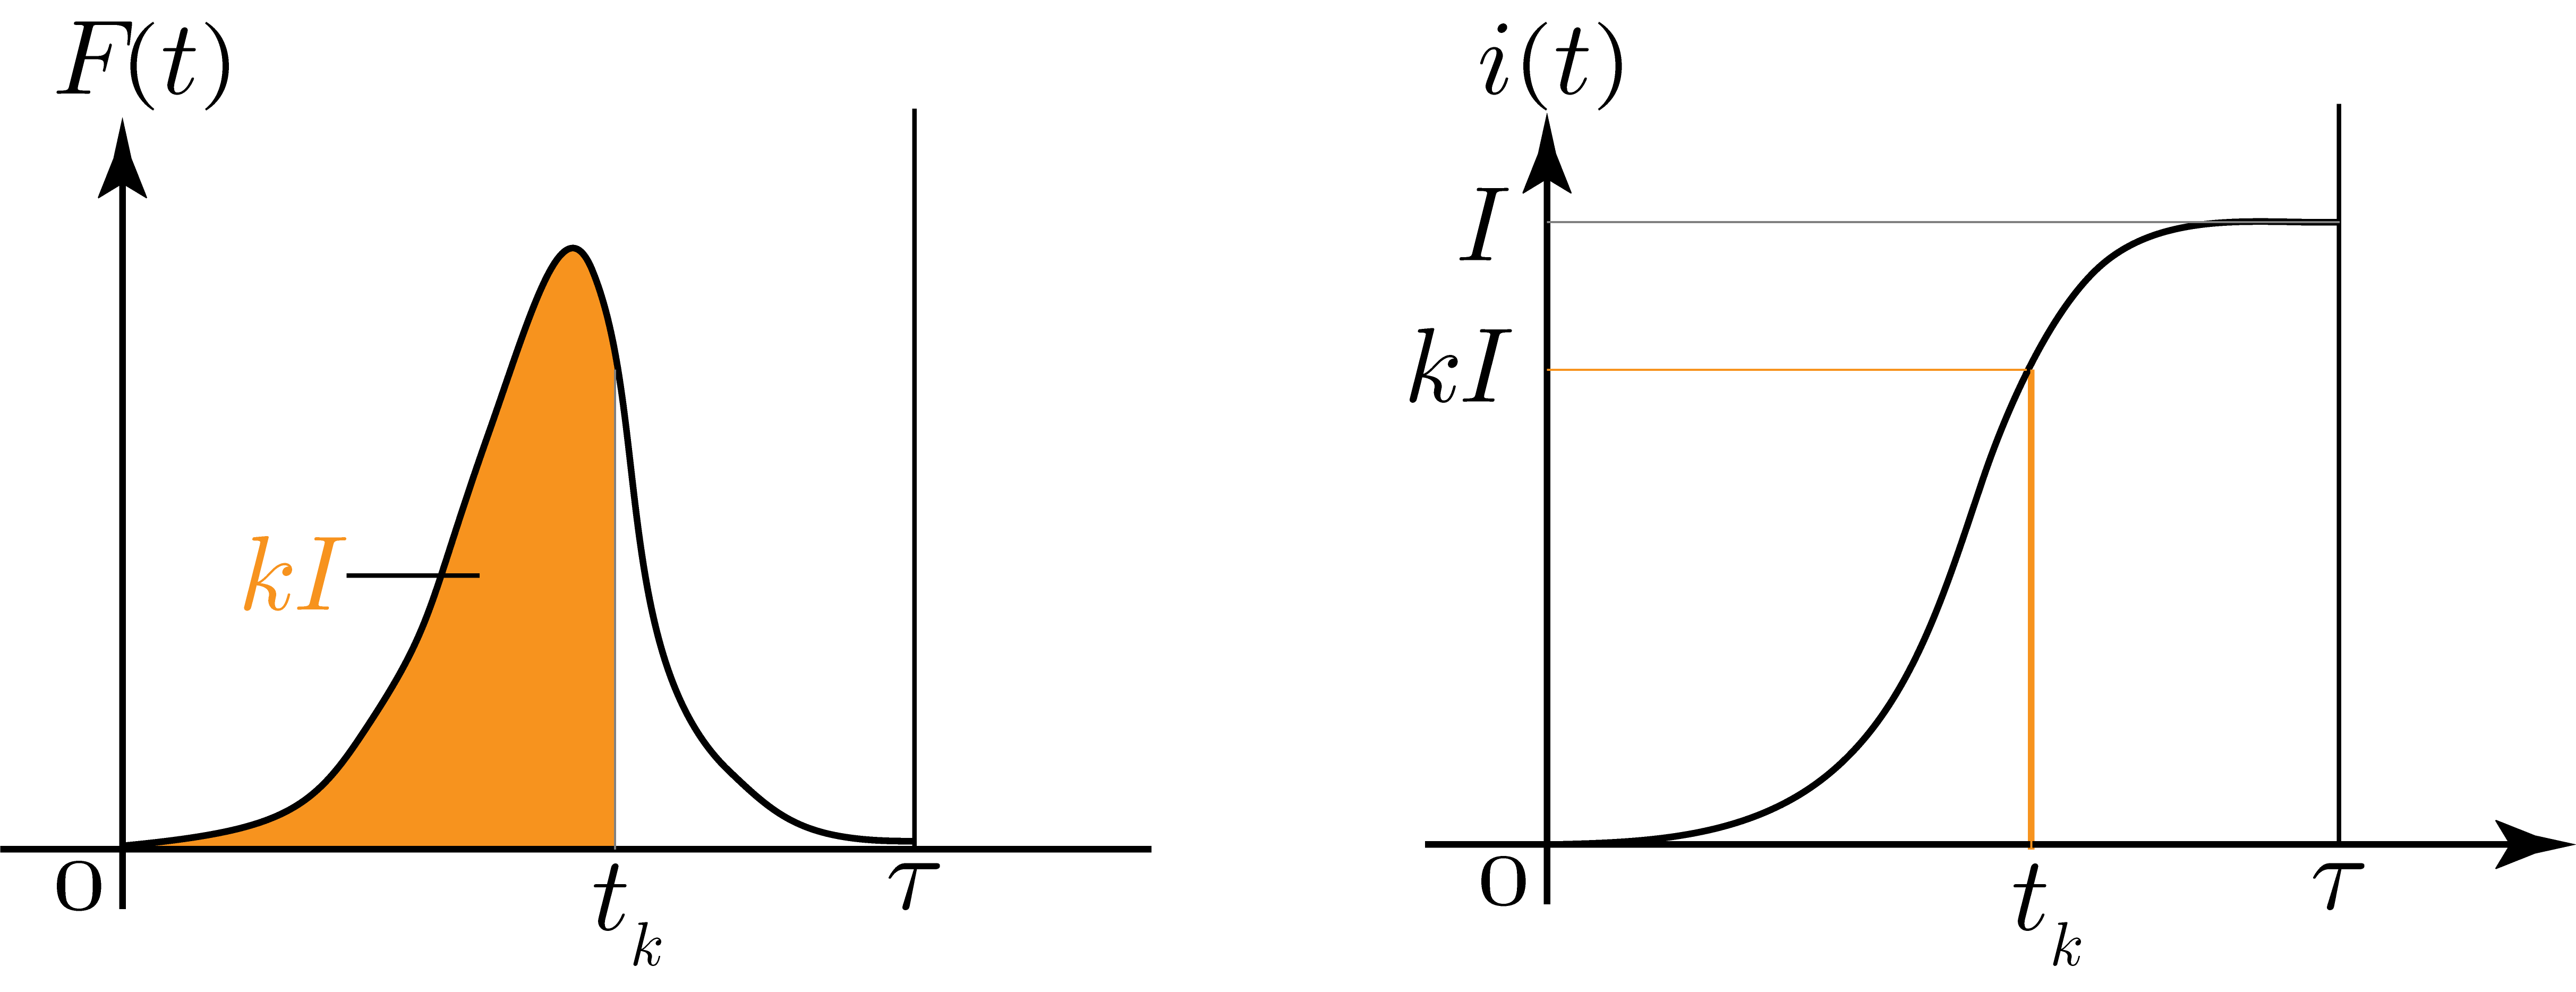
\includegraphics[width=16cm]{image/6-1-12.png}
\caption{力与累积的冲量}
\end{figure}


虽然这个问题倒是也分析地清,\,但这足以告诉我们,\,选取一个简单清晰的模型的必要性.\,为此我们进一步设出碰撞过程中两质点之间持续作用的力$F(t)$,\,它从$0$时刻开始产生到$\tau$时刻作用结束.\,但是,\,并不是只有两质点直接接触才发生作用力,\,事实上我们可以人为把这两个力加在相距较远的两个质点上,\,用这样的模型去等效本来可能复杂的碰撞过程.

我们再把过程中累积的冲量定义为一个函数:
\[i(t)=\int_0^t F(t')\ud t'\]

并且把最终造成的总作用冲量记作$I$:
\[I=\int_0^\tau F(t')\ud t'\]

那就必然有一个时刻冲量累积到$kI$,\,可以把这个时刻记作$t_k$,\,即:
\[i(t_k)=kI\]

事实上由于$i$是严格单调的增函数,\,就存在反函数$i^{-1}$,\,那么这个时间就是:
\[t_k=i^{-1}(kI)\]

有$i^{-1}(0)=0,\,i^{-1}(I)=\tau$.\,这样就足够我们去计算过程中相互作用力的做功了.\,由于是真实碰撞的模拟,\,那么必然$v_1\geq v_2$碰撞才可以发生.\,当冲量累积到$i$时,\,两个质点的速度分别为:
\[u_1=v_1-\frac{i}{m_1}\]
\[u_2=v_2+\frac{i}{m_2}\]

这说明过程$1$速度不断减小,\,$2$速度不断增加.\,现在就足够写出力对$1$和$2$做功的功率了.\,分别为:
\[P_1=-Fu_1=-\frac{\ud i}{\ud t}\left(v_1-\frac{i
}{m_1}\right)\]
\[P_2=Fu_2=\frac{\ud i}{\ud t}\left(v_2+\frac{i
}{m_2}\right)\]

最后如果把功率对时间积分,\,我们发现积分自动以$i$为自变量了:
\[W_1=\int_0^\tau P_1(t)\ud t=-\int_0^I \left(v_1-\frac{i
}{m_1}\right)\ud i\]
\[W_2=\int_0^\tau P_2(t)\ud t=\int_0^I \left(v_2+\frac{i
}{m_2}\right)\ud i\]

线性函数的积分,\,就等于函数值初末值的平均值乘以积分区间的长度,\,这就给出了一个\emph{冲量乘速度形式的功},\,碰撞过程中相互作用力对质点1和质点2的功应当是:
\[W_1=-\frac{1}{2}I(v_1+v_1')\]
\[W_2=\frac{1}{2}I(v_2+v_2')\]

这并不是任何让人意外的结论,\,如果带入动量定理$I=m_1(v_1-v_1')=m_2(v_2'-v_2)$就能发现这两个功无非就是末动能减初动能,\,其实就是反映了动能定律.\,不过注意到表达式推导过程中对动量定律的应用我们发现这个表达式倒不是纯粹的任意情况下都通用的功的定义.\,在使用动量定律前的这个功的积分:
\[W=\int \bs{v}\cdot \ud \bs{I}\]

倒是的确通用的.

如果定义碰前接触速度$v=v_1-v_2$,\,碰后分离速度$v'=v_2'-v_1'$.\,我们可以发现:
\[W_1+W_2=\frac{1}{2}I(v'-v)\]

又定义恢复系数$e=v'/v$.\,碰撞就因此分为四类:

1.\,完全非弹性碰撞,\,$I$最小的情况,\,作为一个实际的碰撞过程分离速度必然也至少为零$v_2'\geq v_1'$,\,否则1仍然在接近2力就不可能会消失.\,所以$I$最小就是让碰撞后共速,\,这样$e=0$就是完全非弹性碰撞的决定$I$大小的条件.

2.\,完全弹性碰撞.\,考虑碰撞过程的能量转化,\,显然,\,如果$W_1+W_2$不等于零,\,前后的总动能就不会是不变量.\,但是如果要求碰前碰后动能不变,\,这就构成了完全弹性碰撞,\,简称弹性碰撞.\,此时,\,除了可以列动能不变来求解$I$,\,我们发现这等价于$v=v'$,\,也就是\emph{接触速度等于分离速度}.\,以后我们将总是认为弹性碰撞的等价对应条件是$e=1$.

3.\,非弹性碰撞(不完全的).\,这是最符合实际情况的一类碰撞.\,这种碰撞中$0<e<1$.\,也就是$v'<v$的情况.\,功$W_1+W_2$是小于零的,\,说明碰撞过程动能有损失,\,能量去向是显而易见的:\,变成了两个碰撞的物体的内能,\,这里的内能可能就是热学上的内能,\,也可以是视作弹性体时虽然整体动量为零但局部有弹性波而产生的宏观动能与势能.\,这种情况之所以普遍是因为,\,碰前往往整个物体没有这样的弹性波,\,能量处于最低的状态,\,碰后这个能量总是会大于零.\,故能量总是有损失的.

4.\,超弹性碰撞.\,也就是$e>1$.\,碰撞后分离速度大于接触速度.\,因碰撞而获得动能.\,这样的过程也并不少见,\,炸弹的爆炸,\,或者刚刚的人推墙使人动起来都是这种情形.\,特点是别的能量会释放出来转化为动能.\,前提需要注意不能违背动量守恒.





\subsection{自由刚体的碰撞}

如果把两个质点的碰撞换为两个自由刚体相碰撞,\,这里我们只考虑平面情况,\,那么同理碰撞会产生一个冲量$\bs{I}$.\,但是这个冲量却有两种可能性,\,如果是光滑的刚体,\,那么碰撞的冲量必然沿法线$n$方向.\,但是如果是粗糙的刚体,\,那么还可以有沿切线方向的分量.\,不管何种情况我们来证明两个恒成立的结论:
\begin{wrapfigure}[14]{o}[-10pt]{6cm}\label{6-1-12}
\centering
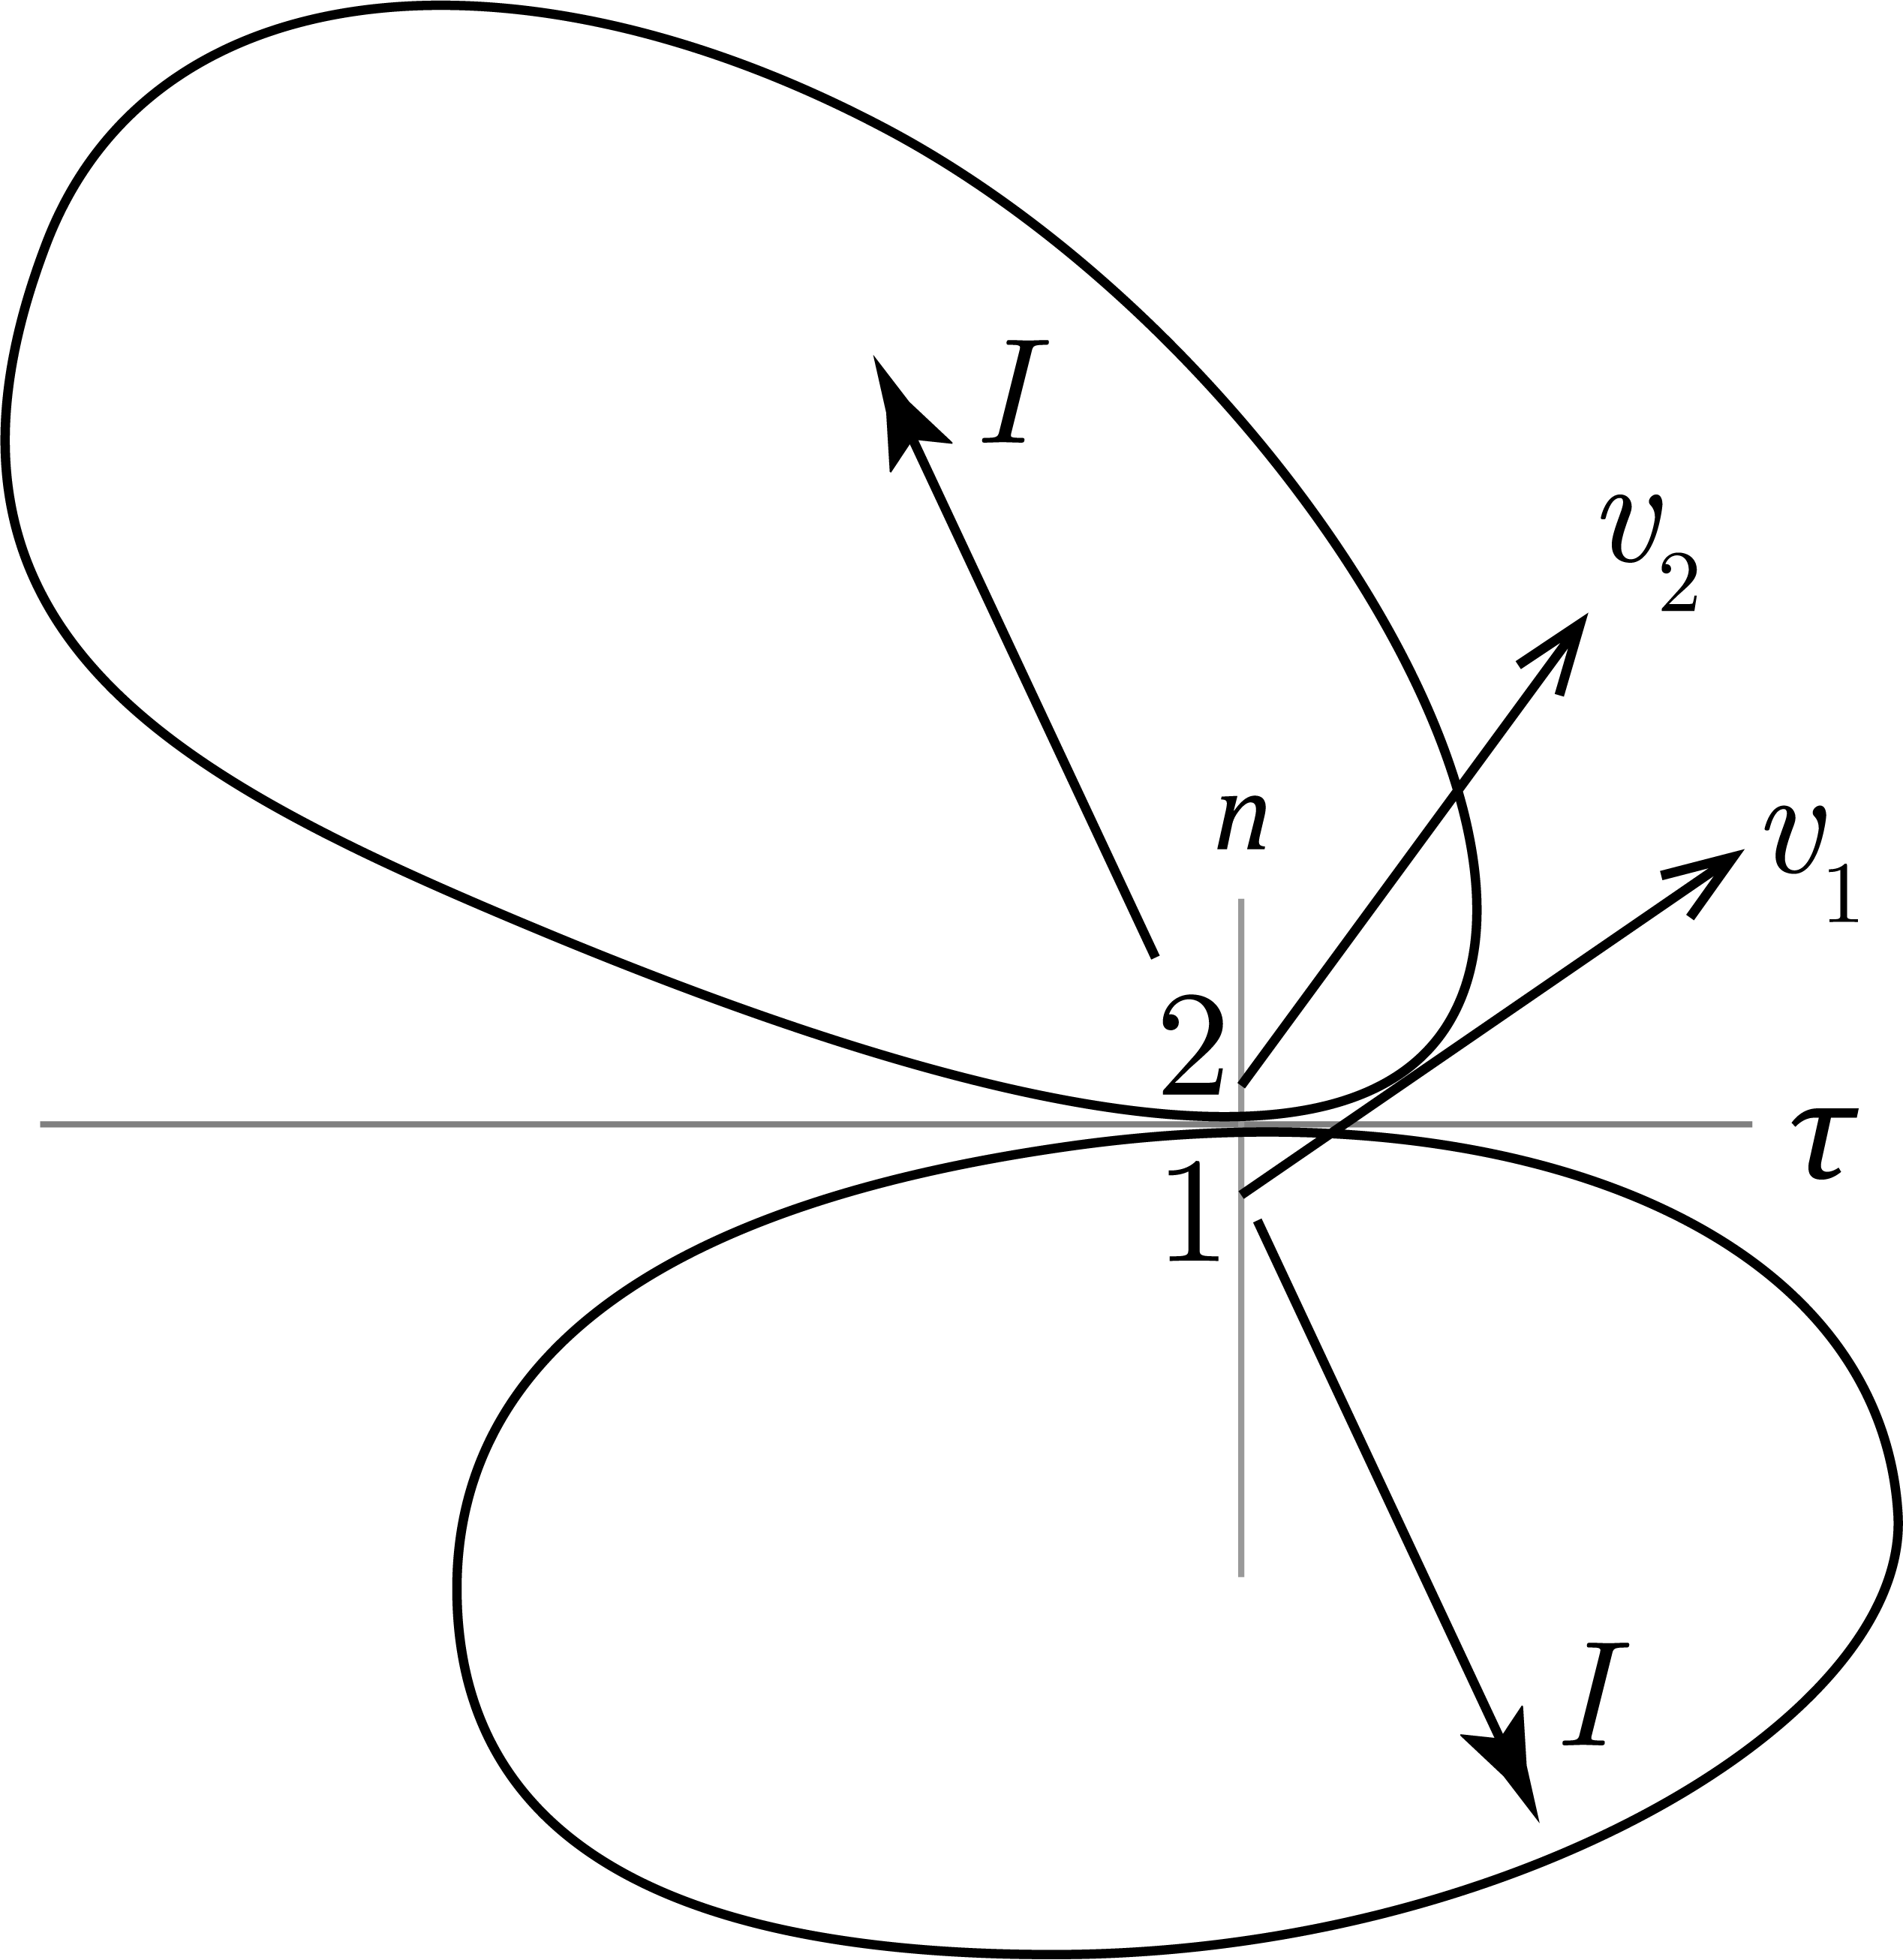
\includegraphics[width=6cm]{image/6-1-13.png}
\caption{两刚体碰撞}
\end{wrapfigure}

一是,\,1对2做的功或2对1做的功总是满足:
\[W=\frac{1}{2}\bs{I}\cdot(\bs{v}+\bs{v}')\]

这里$\bs{v}$和$\bs{v}'$指的便是力的作用点,\,即固连在刚体上的点的速度.\,证明这个定理思路类似于之前的做法.\,我们可以为过程中的冲量累计选取一个变量$k(t)$.\,当$k=0$时碰撞刚刚开始,\,而$k=1$时碰撞就结束了.\,变量取$k$时作用的冲量为:
\[\bs{i}(t)=k(t)\bs{I}\]

那么由于冲量对刚体质心速度和刚体旋转角速度的影响都是线性的,\,而且碰撞点速度也将线性依赖于这些值.\,从而积累到变量$k$时,\,点具有速度:
\[\bs{u}=k\bs{v}'+(1-k)\bs{v}\]

于是利用做功的积分式:
\[W=\int_0^\tau \bs{F}\cdot \bs{u}\ud t=\int_0^{\bs{I}} \bs{u}\cdot \ud \bs{i}=\int_0^1[k\bs{v}'+(1-k)\bs{v}]\cdot\bs{I}\ud k=\frac{1}{2}\bs{I}\cdot(\bs{v}+\bs{v}')\]

二是,\,不损失机械能的条件是,\,或者更特殊地,\,在无摩擦的碰撞中弹性碰撞的条件是,\,接触点形成的沿冲量方向的接触分速度等于该方向的分离分速度.\,这个证明也是简单的.\,只需要把点乘式后面的速度分解在冲量方向并把两个功相加为零即可.\,也就是我们有广义的$e=1$与动能不变作为弹性碰撞的等价条件.


\subsection{多体碰撞}
如果碰撞是多体的往往有两种不同的处理思路:\,一是屡次碰撞的思路,\,最典型的碰撞就是牛顿摆情况,\,小球与多个连续放置的小球的碰撞如果视作屡次的弹性碰撞就能解释体系形成周期性运动的原因.\,因为两个质量相等的小球的碰撞总是简单的交换速度.\,此时我们注意到碰撞结束后,\,最左侧的两球之间从接触速度的$v$变成了$0$,\,而最右侧的两小球却从$0$变成了$v$:
\begin{figure}[H]
\centering
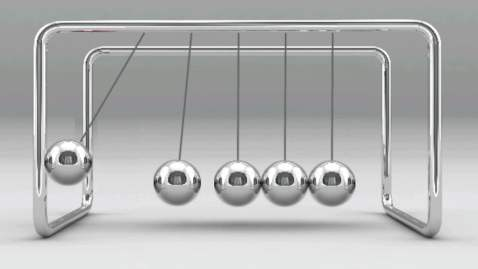
\includegraphics[width=16cm]{image/6-1-14}
\caption{牛顿摆}
\end{figure}

但是如果把最右边的小球要撞击的四个小球视作一个带约束的整体,\,显然既然四个小球必须作为一个整体运动,\,它们之间的相互作用冲量是不会做功的.\,同样的道理也适用于任何带约束的多体碰撞场合,\,虽然碰撞涉及多个物体,\,但是真正具有接触速度的只有一个碰撞点,\,那么作为约束其它点处不可能产生分离速度.\,从而动能不损失的条件依然是在撞击的点处法向接触速度等于分离速度.

不难理解,\,实际的多体碰撞总是介于两种极端情形之间的.\,如果是无限多个无限小的球无限密排,\,这就变成了一个连续的弹性介质中的波动的解的问题,\,波的传播速度和碰撞速度之间的大小关系就成为了一个具有决定性意义的因素.\,容易分析,\,思路一适用与撞击速度很快四个小球还来不及达到平衡的情况.\,而思路二适用于波的传播速度非常快,\,任何冲量作用在四个小球上都相当于在推动四个球构成的整体的情况.
% %!TEX root = ../physical-olympics-2.tex
\chapter{静力学}

以运动学和动力学理论为基础,\,时不时地,\,我们发现一些典型的现象,\,包括:
\begin{itemize}
	\item 不管体系多么复杂,\,能量函数对其行为似乎起决定性的作用.
	\item 似乎总是能够从不同的体系中抽象出它的一个特征数字:\,自由度.
	\item 约束越多体系约复杂,\,它的未知约束力越来越多,\,但是多到一定程度体系只剩下一个自由度了反而用能量守恒就能够解答大多数问题.
\end{itemize}

这些现象无疑是紧密联系的,\,值得研究的.\,事实上我们要做的就是以之前的所有动力学定律为依据进一步展开讨论.\,再从头开始建立新的理论:\,先讨论运动的描述,\,再单独研究力的特性.\,最后合到一起,\,看看这能让我们得到什么.

\section{约束}

\section{力系化简}

\section{平衡问题}

\section{虚功原理}

\section{分析力学初步}

\section{平衡态稳定性}

% %!TEX root = ../physical-olympics-2.tex
\chapter{简谐振动}


\section{方程与谐振}

\subsection{简谐振动的定义}
振动是最常见的物理现象.\,而振动中的最简单(simple)而和谐(harmonic)者谓之\emph{简谐振动}(simple harmonic oscillation).\,对\emph{谐振子}(harmonic oscillator)的学习与研究是会贯彻整个物理理论不同层次内容的始终的.\,现在是经典力学,\,以后会上升到场论,\, 量子力学与量子场论的高度.

简谐振动是指一个物理量$Q$随时间围绕其平衡位置做上下的波动.\,其形式符合:
\[Q=Q_0+\Delta Q\cos(\omega t+\varphi)\]

我们经常会有用复数表示振动的习惯,\,其做法是在三角函数$\cos$与其\emph{宗量}(argument)\,$\phi=\omega t+\varphi$构成的项后添加一个虚的$\ui \sin\phi$项,\,于是新的写法变成:
\[\tilde{Q}(t)=Q_0+\Delta Q\ue^{\ui(\omega t+\varphi)}\; ; \; Q=\mathfrak{Re}(\tilde{Q})\]

又或者:
\[\tilde{Q}(t)=Q_0+\Delta \tilde{Q}\ue^{\ui\omega t}\; ; \; \Delta \tilde{Q}=\Delta Q\ue^{\ui\varphi}\]

以上各个常量中,\,$Q_0$是平衡位置,\,$\Delta Q$叫\emph{振幅}(amplitude),\,宗量$\omega t+\varphi$叫做\emph{相位}(phase),\,$\omega$叫\emph{角频率}(angular frequency),\,$\varphi$叫初相位.\,$\tilde{Q}$为复化的复物理量,\,而$\Delta \tilde{Q}$叫做\emph{复振幅}(complex amplitude).

复数表示最大的一个好处就在于很方便计算物理量的线性组合与导数.\,事实上,\,如果合理选取$Q_0=0$:
\[\dot{Q}=-\omega\Delta Q\sin\phi\; ; \; \dot{\tilde{Q}}=\ui\omega\tilde{Q}\quad \Rightarrow\quad \dot{Q}=\mathfrak{Re}(\dot{\tilde{Q}})\]
\[\ddot{Q}=-\omega^2\Delta Q\cos\phi\; ; \; \ddot{\tilde{Q}}=-\omega^2\tilde{Q}\quad \Rightarrow\quad \ddot{Q}=\mathfrak{Re}(\ddot{\tilde{Q}})\]

\subsection{简谐振动的性质}
以一个质点水平坐标$x$围绕$x=0$左右做谐振为例.\,其运动方程写作\footnote{以后我们对物理量和物理量的复化只在必要的时候加以区分,\,看到复数只需要认为省写了取实部这一例常操作罢了.}:
\[x=A\ue^{\ui(\omega t+\varphi)}\]

那么其速度与加速度为:
\[v=\ui\omega A\ue^{\ui(\omega t+\varphi)},\,a=-\omega^2A\ue^{\ui(\omega t+\varphi)}\]

我们发现在运动过程中的任意一个时刻,\,加速度都是指向平衡位置的,\,与偏离平衡位置的位移是成正比的:
\[a=-\omega^2 x\]

而任意一个时刻既然$x$是宗量的余弦函数,\,$v$是正弦函数,\,它们就满足其绝对值大小的``此消彼长''关系\footnote{注意到这里(往下)要避免使用复数,\,因为一个复数的实部平方不会等于其平方的实部$v^2\neq\mathfrak{Re}(\tilde{v}^2)$}:
\[v^2+\omega^2 x^2=\omega^2 A^2\]

相位是很重要的物理概念,\,\emph{相}(phase),\,状态也,\,相位则是一个可以用来表示状态的数.\,反过来,\,我们可以根据物体在一个时刻的状态反过来确定这个时刻的相位.\,如果位移是$x$而振幅为$A$,\,则:
\[\phi=\mathrm{Arcsin}\frac{x}{A}\, ,\,\mathrm{Arcsin}\frac{x}{A}\in \left\{\arcsin\frac{x}{A}+2n\pi|n\in\mathbb{Z}\right\}\cup\left\{\pi-\arcsin\frac{x}{A}+2n\pi|n\in\mathbb{Z}\right\}\]

同理如果已知速度$v$和\emph{速度振幅}(velocity amplitude)\,$\omega A$,\,那么相位为:
\[\phi=\mathrm{Arccos}\frac{v}{\omega A}\, ,\,\mathrm{Arccos}\frac{v}{\omega A}\in \left\{\arccos\frac{v}{\omega A}+2n\pi|n\in\mathbb{Z}\right\}\cup\left\{-\arccos\frac{v}{\omega A}+2n\pi|n\in\mathbb{Z}\right\}\]

相位的取法上具有多值性.\,但是相位随时间的变化我们约定必须是连续的,\,事实上它随时间线性增加.\,也就是说如果前一个状态下相位为$\phi_1$,\,后一个状态下相位为$\phi_2$,\,那么这两个状态间历时:
\[\Delta t=\frac{\phi_2-\phi_1}{\omega}\]

\subsection{简谐振动的判定}

事实上以上的两个关系都可以成为体系做简谐振动的判据,\,它们为:

\begin{itemize}
	\item 线性回复判据:\,如果一个随时间演化的变量的二阶导数正比于变量本身,\,且符号相反,\,可以判断变量做简谐振动:
	\[\ddot{q}=-\omega^2 q\quad \Rightarrow \quad q=A\cos(\omega t+\varphi)\]

	\item 此消彼长判据:\,如果一个随时间演化的变量的一阶导数与自己的正系数平方和为动力学守恒量(一般就是能量).\,可以判断变量做简谐振动:
	\[\dot{q}^2+\omega^2 q^2=\omega^2A^2\quad \Rightarrow \quad q=A\cos(\omega t+\varphi)\]
\end{itemize}

证明如下:

线性回复$\Rightarrow$此消彼长:

首先进行代换:

\[\ddot{q}=\frac{\ud}{\ud t}(\dot{q})=\frac{\ud q}{\ud t}\frac{\ud}{\ud q}(\dot{q})=\frac{\dot{q}\ud\dot{q}}{\ud q}\]

将上式代入$\ddot{q}=-\omega^2 q$:
\[\dot{q}\ud\dot{q}+\omega^2 \cdot q\ud q=\ud(\frac{1}{2}\dot{q}^2+\frac{1}{2}\omega^2 q^2)=0\quad \Rightarrow \quad \dot{q}^2+\omega^2 q^2=C\]

命$A=\sqrt{C/\omega^2}$即得到此消彼长判据.

此消彼长$\Rightarrow$简谐振动:

考虑$\dot{q}$的正根即可,\,负根结果也是简谐振动:
\[\dot{q}=\frac{\ud q}{\ud t}=\omega\sqrt{A^2-q^2}\]
\[\Rightarrow \quad \frac{\ud q}{\sqrt{A^2-q^2}}=\omega \ud t\]

两边同时积分,\,积分常数写到右侧记作$\varphi$,\,得到:
\[-\arccos \frac{q}{A}=\omega t+\varphi \quad \Rightarrow\quad q=A\cos(\omega t+\varphi)\]
\vspace{-0.1cm}


\subsection{小振动}

值得注意的是,\,很多情况下体系的运动并不是严格的简谐振动.\,十分常见的一种情况是\emph{小振动}(small oscillation).\,事实上,\,如果我们研究体系为完整而稳定的一自由度体系,\,广义坐标为$q$,\,而且势能函数$V(q)$存在一个极小值:
\[V'(q_0)=0\quad,\quad V''(q_0)>0\]

那么根据上一章的阐述,\,这个$q_0$就是体系的稳定平衡位置.\,那么,\,任何偏离这个平衡位置的系统运动只要偏离的值足够小,\,即做坐标变换$\delta=q-q_0$为无穷小量,\,那么就一定为简谐振动.\,这是因为势能可以由泰勒展开为:
\[V=\frac{1}{2}V''(q_0)\delta^2+\frac{1}{3!}V'''(q_0)\delta^3+\cdots\]

只要$\delta$足够小,\,三阶项就必然远小于二阶项.\,从而可以只保留第一项.\,同理这也适用于动能,\,它必然正比于$\dot{\delta}$的平方,\,系数则与平衡位置有关:
\[T=\frac{1}{2}M(q_0)\dot{\delta}^2\]

从而这个体系的能量函数(哈密顿量)就被近似为了:
\[H=T+V=\frac{1}{2}M(q_0)\dot{\delta}^2+\frac{1}{2}V''(q_0)\delta^2\]

这就直接符合了``此消彼长''判据.\,从而小振动的角频率为:
\[\omega=\sqrt{\frac{V''(q_0)}{M(q_0)}}\]

例如,\,在典型的单摆问题中,\,取摆线与竖直方向的夹角$\theta$为广义坐标.\,摆球的重力势能以平衡位置为原点表示为:
\[V(\theta)=mgl(1-\cos\theta)\]

而动能为:
\[T=\frac{1}{2}ml^2\dot{\theta}^2\quad \Rightarrow\quad M(\theta)=ml^2\]

从而只需要带入以上公式,\,就得到:
\[\omega=\sqrt{\frac{V''(0)}{M(0)}}=\sqrt{\frac{mgl}{ml^2}}=\sqrt{\frac{g}{l}}\]

这是因为事先看出来了稳定平衡点为$\theta=0$.\,简单的小振动问题的思路都大抵如此.\,第一步是写出能量函数来,\,它决定体系的所有可能的动力学演化.\,第二步要找到稳定平衡位置,\,往往一样地是通过势能函数的增减凹凸性来判断,\,往往也要结合体系的对称性来观察.\,最后便是在平衡位置处把动能势能都近似为简单的平方项.\,唯一需要补充的是,\,除了利用二阶导数来计算这一个平方项,\,对常见函数写泰勒展开式也是十分常见的思路.

单摆问题的周期从而就是:
\[T=\frac{2\pi}{\omega}=2\pi\sqrt{\frac{l}{g}}\]

但是一定要注意这个振动仅仅对小振动成立.\,例如在摆角为$10\dgr=0.087{\rm rad}$时会有约$2\permil$的误差.\,如何计算这个误差?\,之后的非线性振动将讨论这个问题.


\section{阻尼振动与受迫振动}

\subsection{阻尼振动}

阻尼振动,\,狭义地是指普通的弹簧型谐振子,\,但是让振子运动的空间充满介质而产生湿摩擦(流体摩擦).\,从而产生一个正比于速度的阻尼的情形.\,其牛顿定律为:
\[m\ddot{x}=-kx-\gamma \dot{x}\]

这里的$\gamma$即\emph{阻尼系数}(damping coefficient).\,习惯上把$m/\gamma$称作\emph{弛豫时间}(relaxation time).\,最后还定义\emph{衰减参数}(attenuation parameter)或\emph{损耗参数}(loss parameter)为:
\[\beta=\frac{\gamma}{2m}\]

而无阻尼情况下的\emph{固有频率}(natural frequency), 这里是角频率,\,为:
\[\omega_0=\sqrt{\frac{k}{m}}\]

这样原来的方程又被重新写为:
\[\ddot{x}+2\beta \dot{x}+\omega_0^2 x=0\]

我们定义广义的\emph{阻尼振动}(damped oscillation),\,只需要一个运动的任意自由度$q$,\,符合或者可以近似为以上式子形式的动力学方程,\,那么这个自由度上的运动就是一个阻尼振动.\,所有的阻尼振动只有两个常数特征,\,一个是固有角频率,\,一个是损耗的大小.

\vspace{1cm}
阻尼振动的求解需要分为三种情况.\,我们统一猜解:
\[x=A\ue^{\ui\omega t}\]

带入原方程以后发现$\omega$需要满足:
\[\omega^2-2\ui\beta\omega-\omega_0^2=0\]

从而:

\begin{itemize}
	\item \emph{欠阻尼}(underdamped)

	常见的小阻尼情况,\,此时$0<\beta<\omega_0$.\,通过对以上方程求解得到两个含有正虚部的关于虚轴对称的根:
	\[\omega_{1,2}=\ui\beta \pm\sqrt{\omega_0^2-\beta^2}\]

	这样就得到了原阻尼振动方程的通解:
	\[x=\ue^{-\beta t}[A\cos(\sqrt{\omega_0^2-\beta^2}t)+B\sin(\sqrt{\omega_0^2-\beta^2}t)]=C\ue^{-\beta t}\cos(\sqrt{\omega_0^2-\beta^2}t+\varphi)\]

	\begin{figure}[H]
	\centering
	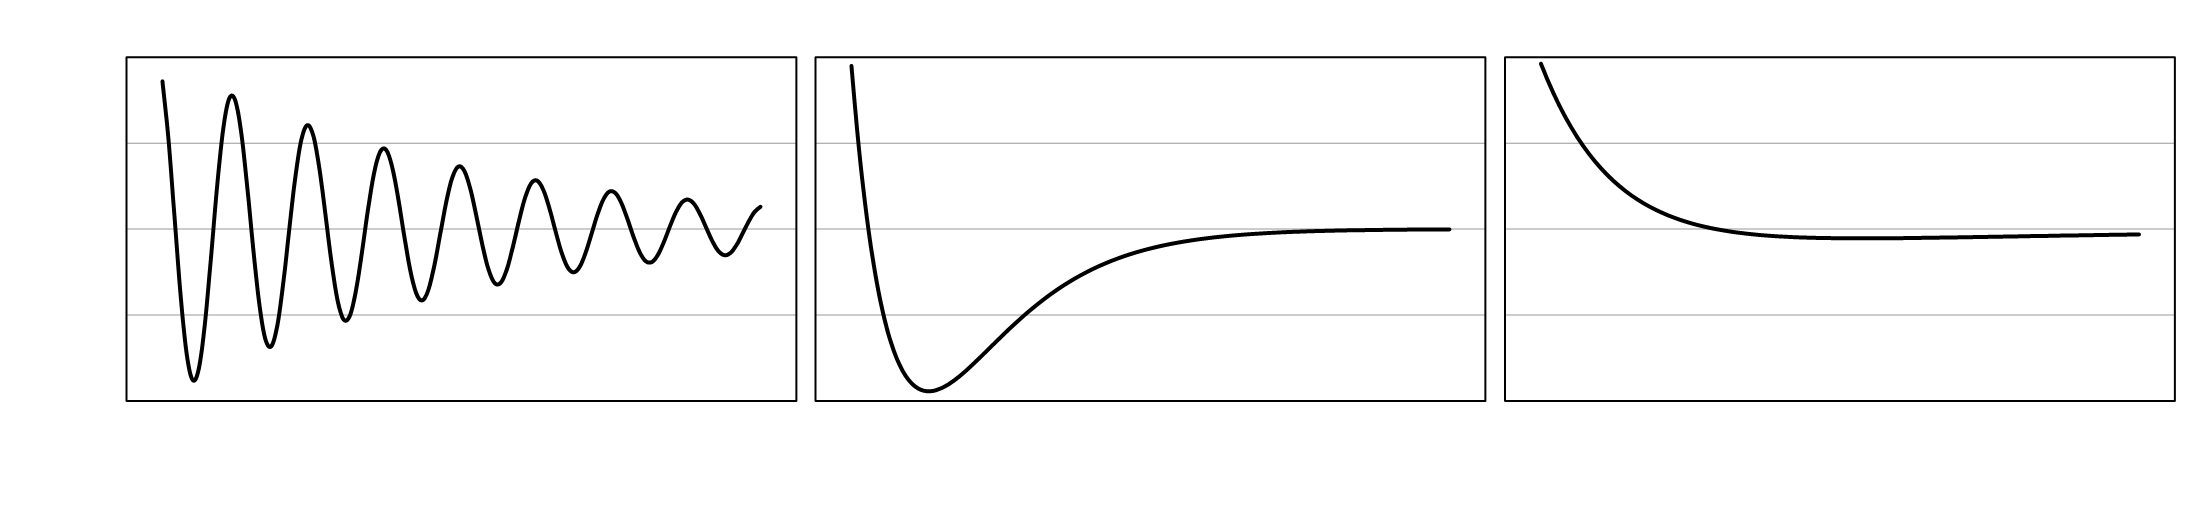
\includegraphics[width=14cm]{image/6-3-1.png}
	\caption{欠阻尼, 临界阻尼与过阻尼}
	\end{figure}

	\item \emph{过阻尼}(overdamped)

	此时$\beta>\omega_0$.\,从而振动和回复力被极大地抑制了.\,主要是一个在大阻力和初速度下缓慢回到平衡位置的运动.\,以上方程两根此时为两个正虚根:
	\[\omega_{1,2}=\ui(\beta\pm\sqrt{\beta^2-\omega_0^2})\]

	这样就得到了原阻尼振动方程的通解:
	\[x=\ue^{-\beta t}[A\ue^{\sqrt{\beta^2-\omega_0^2}t}+B\ue^{-\sqrt{\beta^2-\omega_0^2}t}]=C\ue^{-\beta t}\cosh(\sqrt{\beta^2-\omega_0^2}t+\varphi)\footnote{也有可能是$\sinh$}\]

	\item \emph{临界阻尼}(critical damped)

	这对应$\beta=\omega_0$的特殊情况.\,可以通过微分方程的理论,\,或者采用求$\beta\to \omega_0$极限的方式得到此时的运动方程.\,它为:
	\[x=\ue^{-\beta t}(A+Bt)\]

	临界阻尼在实际生活中的应用为:\,它是较快能够让振子回到平衡位置的理想阻尼大小.\,这一点不难理解,\,不难看出,\,欠阻尼情况的振幅随时间的衰减方式为$\ue^{-\beta t}$,\,也就是适当增大$\beta$有利于振幅尽快衰减.\,但是,\,过阻尼时,\,长时间后位移与时间的关系为
	\[x\sim \ue^{-\beta t}\cosh(\sqrt{\beta^2-\omega_0^2}t)\sim\ue^{-\beta t}\ue^{\sqrt{\beta^2-\omega_0^2}t}\sim \ue^{-\frac{\omega_0^2t}{\beta+\sqrt{\beta^2-\omega^2}}}\]

	这就不难发现,\,此时增加$\beta$只会使得$t$前的衰减系数变小而不利于尽快衰减其位移.\,从而,\,无论是欠阻尼还是过阻尼,\,临界阻尼是它们能够尽快回到平衡位置的极限.\,此时原来的固有频率对应的周期就是它回到平衡位置的特征时间.
\end{itemize}

对于欠阻尼情况,\,尤其是衰减因子$\beta<<\omega_0$的小阻尼情况,\,还有一些重要的性质值得挖掘.\,下面都默认是这样的前提:

\begin{wrapfigure}[17]{o}[-10pt]{7cm}
\centering
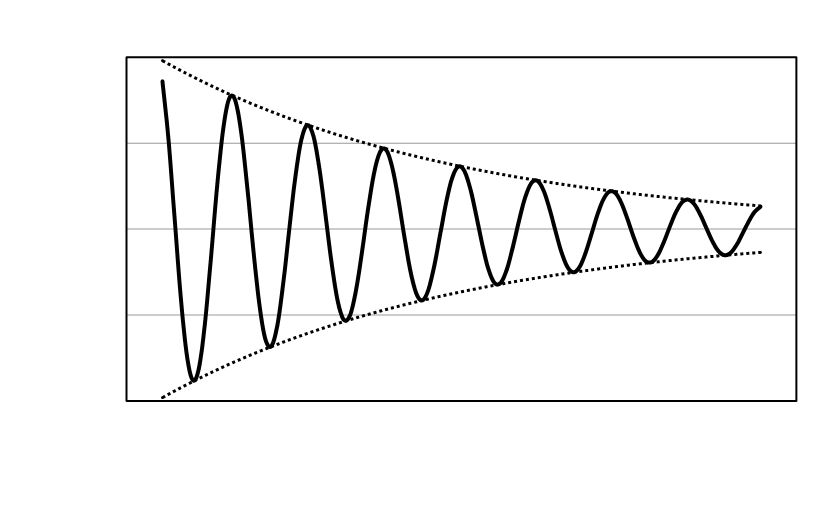
\includegraphics[width=7cm]{image/6-3-2.png}
\caption{\quad 小阻尼下的振幅衰减}
\end{wrapfigure}
从之前的运动方程解不难看出来,\,我们可以把小阻尼情况下的运动方程看作是一个振幅不断随着时间衰减的简谐振动.\,其振幅衰减函数和阻尼化角频率为:
\[A(t)=A_0\ue^{-\beta t}\]
\[\omega_d=\sqrt{\omega_0^2-\beta^2}\approx \omega_0\]

要讨论其衰减的原因,\,还有一种新的角度,\,便是考虑其能量.\,当振幅为$A$时,\,其动能,\,势能的和为:
\[E=T+V=\frac{1}{2}m\dot{x}^2+\frac{1}{2}kx^2\]

现在它不是守恒的,\,仅仅是在少数几个周期里面``近似''守恒.\,但是我们可以考虑求它在一个周期内的平均:
\[\bar{E}=\frac{1}{2}\cdot\frac{1}{2}m\omega_d^2 A^2+\frac{1}{2}\cdot\frac{1}{2} kA^2=\frac{1}{2}m\frac{\omega_0^2+\omega_d^2}{2} A^2\approx \frac{1}{2}m\omega_0^2 A^2\]

现在我们计算单位时间减少的能量的平均值.\,它其实就是阻尼造成的负功功率的平均值:
\[\bar{P}=\overline{\gamma v\cdot v}=\frac{1}{2}\gamma \omega_d^2 A^2\approx \frac{1}{2}\gamma \omega_0^2 A^2=\frac{1}{2}m \omega_0^2 A^2\cdot 2\beta\]

通过损耗功率等于能量的负导数,\,也可以得到振幅随着时间衰减的具体结果.\,我们现在关心一个重要的量,\,它实际上是反应振子振动单位时间所减少的能量占由于以$\omega_0$振动导致的总能量转化速率的比例,\,我们把上式换一种写法:
\[\bar{P}=\frac{\omega_0\bar{E}}{Q}\]

以上引入的$Q$就是著名的\emph{品质因数}(quality factor).\,它越大,\,表示损耗越低,\,振子的阻尼就越小,\,就越接近``谐振''.\,实际上它算法为:
\[Q=\frac{\omega_0}{2\beta}\]

品质因数经常与另一个因子一起提出,\,两者是简单的倒数关系,\,更精确地,\,我们定义:
\[\sin\delta=\frac{1}{2Q}=\frac{\beta}{\omega_0}\]

$\delta$被称作\emph{损耗角}(loss angle).\,一定要注意这两个概念是普遍的.\,谐振子模型是很多实际问题的抽象,\,它们作为谐振子都有自己的品质因数或损耗角,\,用以描述过程的一些共性,\,而且,\,不光可以用能量的损失的共性来定义品质因数和损耗角,\,还有很多重要的方式.\,详情见后.

\begin{wrapfigure}[17]{o}[-10pt]{7cm}
\centering
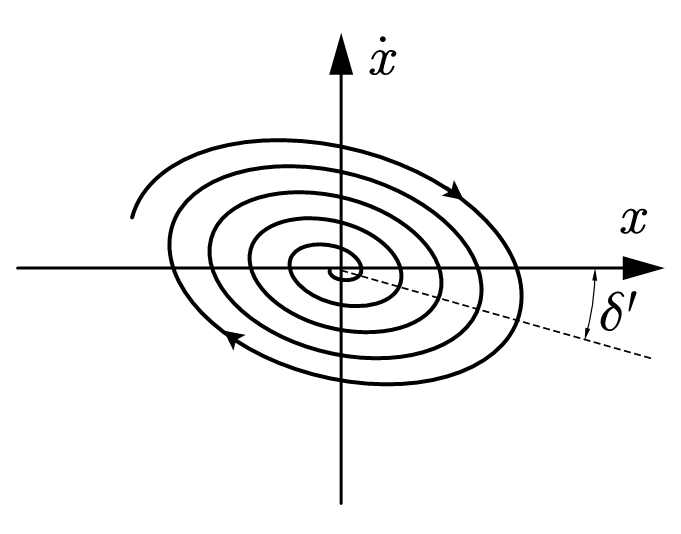
\includegraphics[width=7cm]{image/6-3-3.png}
\caption{阻尼振动的相图}
\end{wrapfigure}
现在我们来考虑简谐振动的\emph{相图}(phase diagram).\,在动力学中,\,这总是指把单个过程的运动,\,画成以其广义坐标和广义速度(或动量)为坐标轴的\emph{相空间}(phase space)中的曲线形成的图像.\,阻尼振动的代表性解为:
\[x=A\ue^{-\beta t}\ue^{\ui \omega_d t}\]

在这个解下,\,其速度为:
\[\dot{x}=(\ui\omega_d-\beta)A\ue^{-\beta t}\ue^{\ui \omega_d t}\]

两个量都在随时间衰减.\,从而在相图上就体现为一随着时间不断向着原点靠近的螺旋线.\,如果没有阻尼,\,那么标准简谐振动的相轨迹就是正椭圆:
\[\frac{x^2	}{A^2}+\frac{\dot{x}^2}{\omega_0^2A^2}=1\]

但是,\,有阻尼时除了是螺旋式的椭圆,\,它还不是``正''的.\,事实上,\,如果去除衰减因子,\,即将$x$和$\dot{x}$乘以个$\ue^{\beta t}$以抵消其衰减:
\[X=x\ue^{\beta t}=A\ue^{\ui \omega_d t}\quad,\quad V=\dot{x}\ue^{\beta t}=\ui(\omega_d+\ui\beta)A\ue^{\ui \omega_d t}\]

两者之间也不是恰好相差相位$\pi/2$,\,而是有一个额外相位差:
\[\delta=\arctan\frac{\beta}{\omega_d}=\arcsin\frac{\beta}{\omega_0}\]

可以发现这个相位差就是损耗角.\,也就是说,\,损耗角的另一种理解方式是位置与速度振动过程中的相位夹角.\,作为结果,\,其相图中的椭圆也要倾斜一个角度$\delta'$.\,可以证明,\,损耗角越大,\,这个倾斜角度也会越大.

\subsection{受迫振动}

如果在谐振子上施加一个周期性的策动外力.\,我们总是研究基本的简谐式的外力\footnote{傅里叶分析理论告诉我们,\,任何函数都可以分解为无穷多助三角函数的线性组合.\,故对于线性系统原则上就可以用叠加原理处理任意任意强迫力的运动求解:\,只要我们把简谐强迫力找到解法.}:
\[F(t)=F_0\ue^{\ui\omega t}\quad {\rm i.e.}\quad F(t)=F_0\cos{\omega t}\]

这个运动就称作\emph{受迫振动}(driven oscillation).\,这样子原来的方程就变为:
\[m\ddot{x}+\gamma\dot{x}+kx=F_0\ue^{\ui\omega t}\]
\[\Rightarrow\quad \ddot{x}+2\beta\dot{x}+\omega_0^2 x=\frac{F_0}{m}\ue^{\ui\omega t}\]

很明显,\,可以猜一个谐振解.\,它是上述微分方程的特解(稳态解).\,通解还需要加上上一部分讨论的阻尼振动解(齐次方程的解是暂态解).\,注意其振动频率应当是策动力的频率$\omega$而不是体系的固有频率$\omega_0$:
\[x=A\ue^{\ui\omega t}\quad \Rightarrow \quad (\omega_0^2-\omega^2+2\ui\beta\omega)A=\frac{F_0}{m}\]

故,\,复振幅的解法也是相当地直接:
\[A=\frac{F_0/m}{\omega_0^2-\omega^2+2\ui\beta\omega}\]


作为复振幅,\,上$A$表达式其实同时包含了两个因素,\,一个是振幅,\,一个是相位.\,现在我们分离它们:
\[A=|A|\ue^{\ui \varphi}\]
\[|A|=\frac{F_0/m}{\sqrt{(\omega_0^2-\omega^2)^2+4\beta^2\omega^2}}\]
\[\varphi=-\arctan\frac{2\beta\omega}{\omega_0^2-\omega^2}\quad {\rm or} \quad \varphi=-\left(\pi-\arctan\frac{2\beta\omega}{\omega^2-\omega_0^2}\right)\]

\begin{wrapfigure}[15]{o}[-10pt]{7cm}
\centering
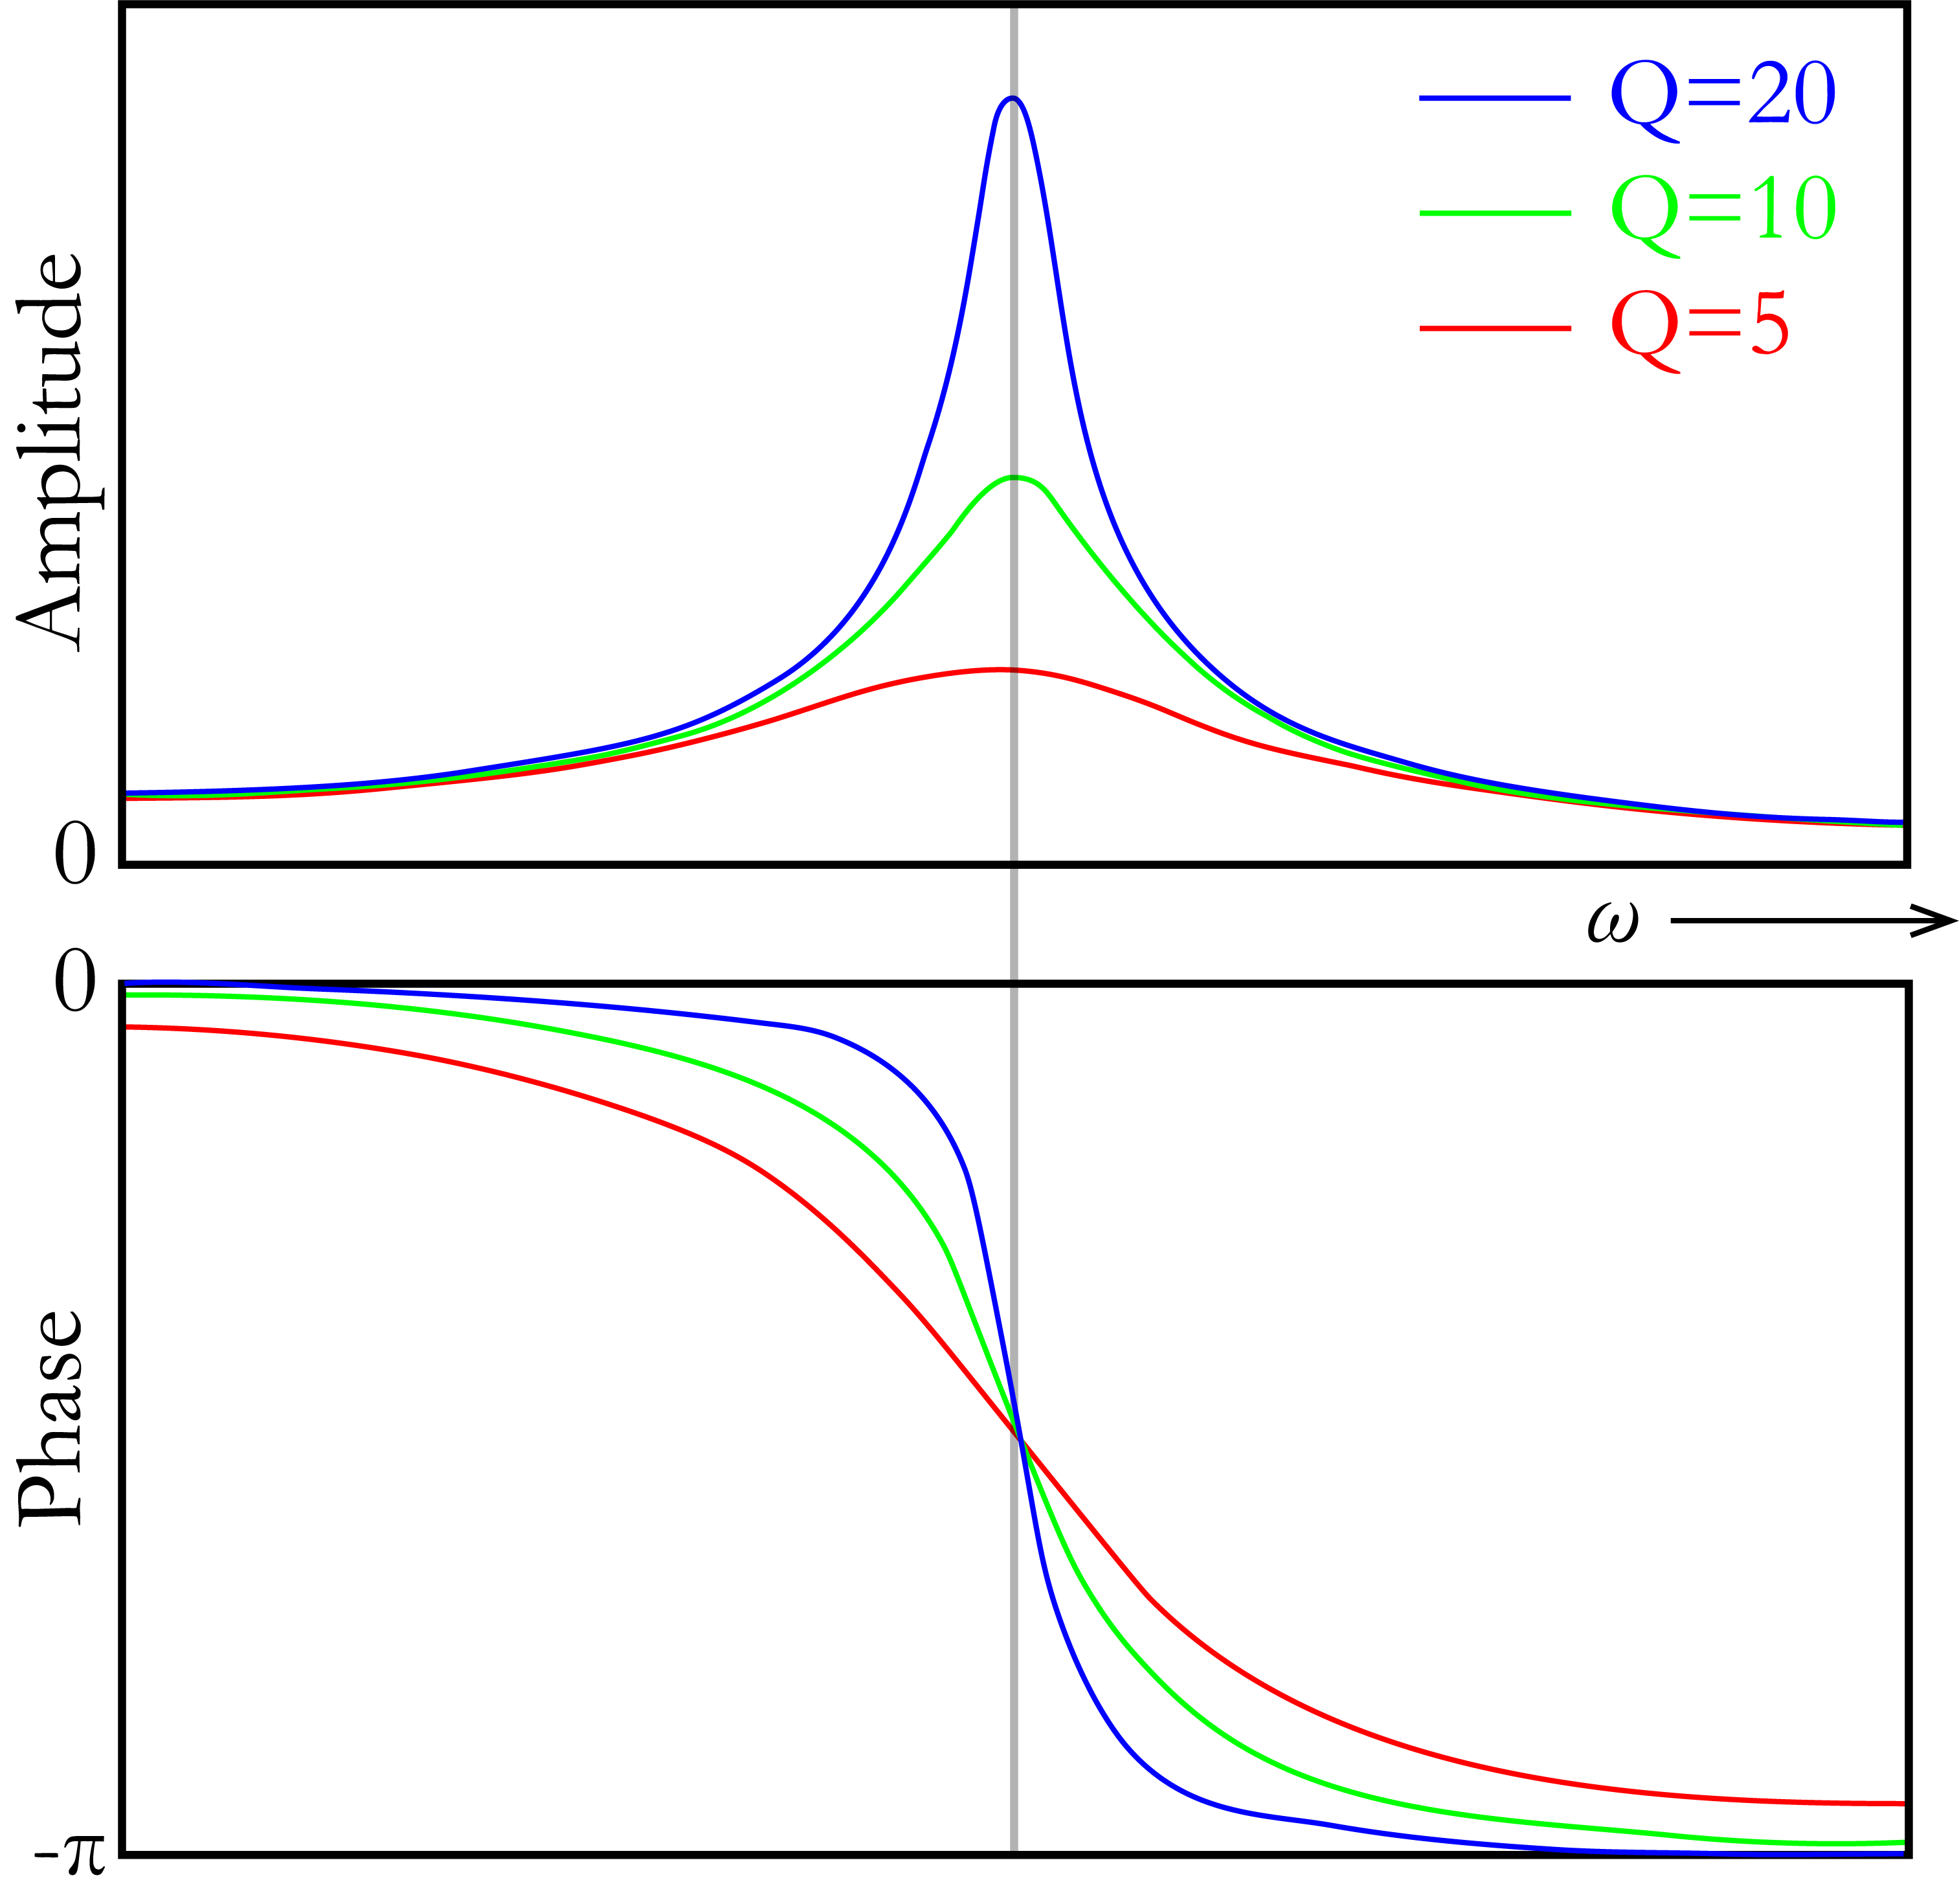
\includegraphics[width=7cm]{image/6-3-4.png}
\caption{幅频, 相频特性}\label{6-3-4}
\end{wrapfigure}
这就构成了两个关于$\omega$的函数.\,这也是实验上我们特别关心的两个函数,\,它们反映在稳态受迫振动的时候,\,一定外力下振子产生的振幅与相位究竟是怎样取决于策动力的角频率的.\,这就是著名的\emph{幅频特性}(amplitude-frequency characteristic)和\emph{相频特性}(phase-frequency characteristic).\,利用之前定义的品质因数$Q$,\,再命$x=\omega/\omega_0$.\,整理得:
\[|A|=\frac{QF_0/m\omega_0^2}{\sqrt{Q^2(1-x^2)^2+x^2}}\]
\[\varphi=-\arccos\frac{Q (1-x^2)}{\sqrt{Q^2(1-x^2)^2+x^2}}\]


我们依然只考虑小阻尼情况.\,此时$Q$较大.\,比如如图\ref{6-3-4}所示,\,$Q=5,\,10,\,20$等.

那么受迫振动又被分为三种情形:

\begin{itemize}
	\item 低频区为弹性控制区.

	在$\omega\ll\omega_0$时,\,$m\ddot{x},\,\gamma\dot{x},\,kx$三项中最后一项最大,\,主要是弹簧的弹性力与策动力去平衡.\,从而体现出以下计算结果:
	\[|A|\approx \frac{F_0}{m\omega_0^2}=\frac{F_0}{k}\]
	\[\varphi\approx 0\]

	也就是策动力与位移几乎同相,\,振子有充分的时间去实现平衡.

	\item 高频区为惯性控制区.

	在$\omega\ll\omega_0$时,\,$m\ddot{x},\,\gamma\dot{x},\,kx$三项中第一项最大,\,主要是高速变化的策动力去直接产生振子加速度.\,从而体现出以下计算结果:
	\[|A|\approx \frac{F_0}{mx^2\omega_0^2}=\frac{F_0}{m\omega^2}\]
	\[\varphi\approx -\pi\]

	也就是策动力与位移几乎反相(亦反向).\,振子``随波逐流'',\,弹性力和阻尼力没有时间跟上策动力的节奏.

	\item 中频区为共振区.

	在$\omega$在$\omega_0$附近,\,即量级接近时.\,三个项$m\ddot{x},\,\gamma\dot{x},\,kx$也量级相当.\,如果把结果画成图\ref{6-3-4}.\,可以发现十分典型的现象是,\,振幅在某频率处取到了极值.\,而相位差(绝对值)在某频率处从小于$\pi/2$增加到大于$\pi/2$.
\end{itemize}

\emph{共振}(resonance)是谐振子系统中十分典型的现象.\,一个共振发生的时候有两个量是值得关注的:

第一个值得关注的共振参数,\,是共振的峰的位置.\,即\emph{共振频率}(resonance frequency).\,但是这个因素又被分为位移共振和速度共振,\,即位移振幅$|A|$最大或者速度振幅最大的角频率值.\,或者可以证明,\,等价的是,\,\emph{振幅共振}(amplitude resonance)和\emph{相位共振}(phase resonance).\,前者指的是响应$x$最大的点:
\[x^2=1-\frac{1}{2Q^2}\approx 1\quad \Rightarrow \quad \omega\approx\omega_0\]

后者则指响应和策动力完全相位差为$\pi/2$的情况:
\[x^2=1\quad \Rightarrow \quad \omega=\omega_0\]

可见两个共振在小阻尼情况下几乎是重合的.\,在振幅共振的情况下,\,振幅最终为:
\[|A|=Q\cdot\frac{F_0}{m\omega_0^2}\cdot\sqrt{\frac{4Q^2}{4Q^2-1}}\approx Q\cdot\frac{F_0}{m\omega_0^2}\]

如果以这个角频率的外力$F_0$直接作用在自由的质点上,\,或者是考虑让一个没有阻尼的振子进行固有振动并使弹簧给振子的力就是$F_0$.\,我们发现振子振幅应当是$F_0/m\omega_0^2$.\,这就是说共振时振幅成为了这个振幅的$Q$倍.\,说明了如果让体系从静止开始,\,自某一时刻开始受到周期性的外力而产生振动,\,如果频率接近固有频率,\,体系会十分反常的振幅越来越大,\,直到振幅是自由振幅的$Q$倍.\,这也是品质因数的第二种理解方式:\,共振的放大倍数.

在看相位共振时的策动力-相位差为$\pi/2$的现象.\,这说明了什么?\,这说明策动力与速度完全就是同相的.\,带入$x=1$容易计算此时位移振幅为$|A|=QF_0/m\omega_0^2$,\,等效地可以写成$F_0=m\omega_0^2|A|/Q$.\,那么速度振幅就是$\omega_0|A|$.\,从而策动力对速度单位时间做的功就是:
\[W=\overline{F(t)\dot{x}(t)}=\frac{1}{2}F_0\omega_0|A|=\left.\frac{1}{2}m\omega_0^3|A|^2\right/ Q\]

这与上一部分得到了相似的结果.\,因为振动的能量其实就是:
\[\bar{E}=\frac{1}{2}m\omega_0^2|A|^2\]

也就是说品质因数反映了耗散的能量与总能量(动能势能互相转换)的比例:
\[Q=\frac{\omega_0 \bar{E}}{W}\]

第二个值得关注的共振参数,\,是共振的峰的宽度.\,谐振子模型给出的幅频曲线,\,与著名的\emph{柯西分布}(Cauchy distribution)对应的函数曲线有密切联系,\,柯西分布又常常因为在理论物理学中的广泛使用而称作\emph{洛伦兹型}(lorentzian shape)\footnote{比如谱线的形状,\,即线型,\,就常被视作洛伦兹线型.}.\,所谓柯西分布最初来自概率分布模型,\,它是指以下分布函数:
\[{\rm pdf.}\footnote{probability distribution function,\,即概率分布函数的缩写.}=\frac{1}{\pi[\gamma^2+(x-x_0)^2]}\]

\begin{figure}[H]
\centering
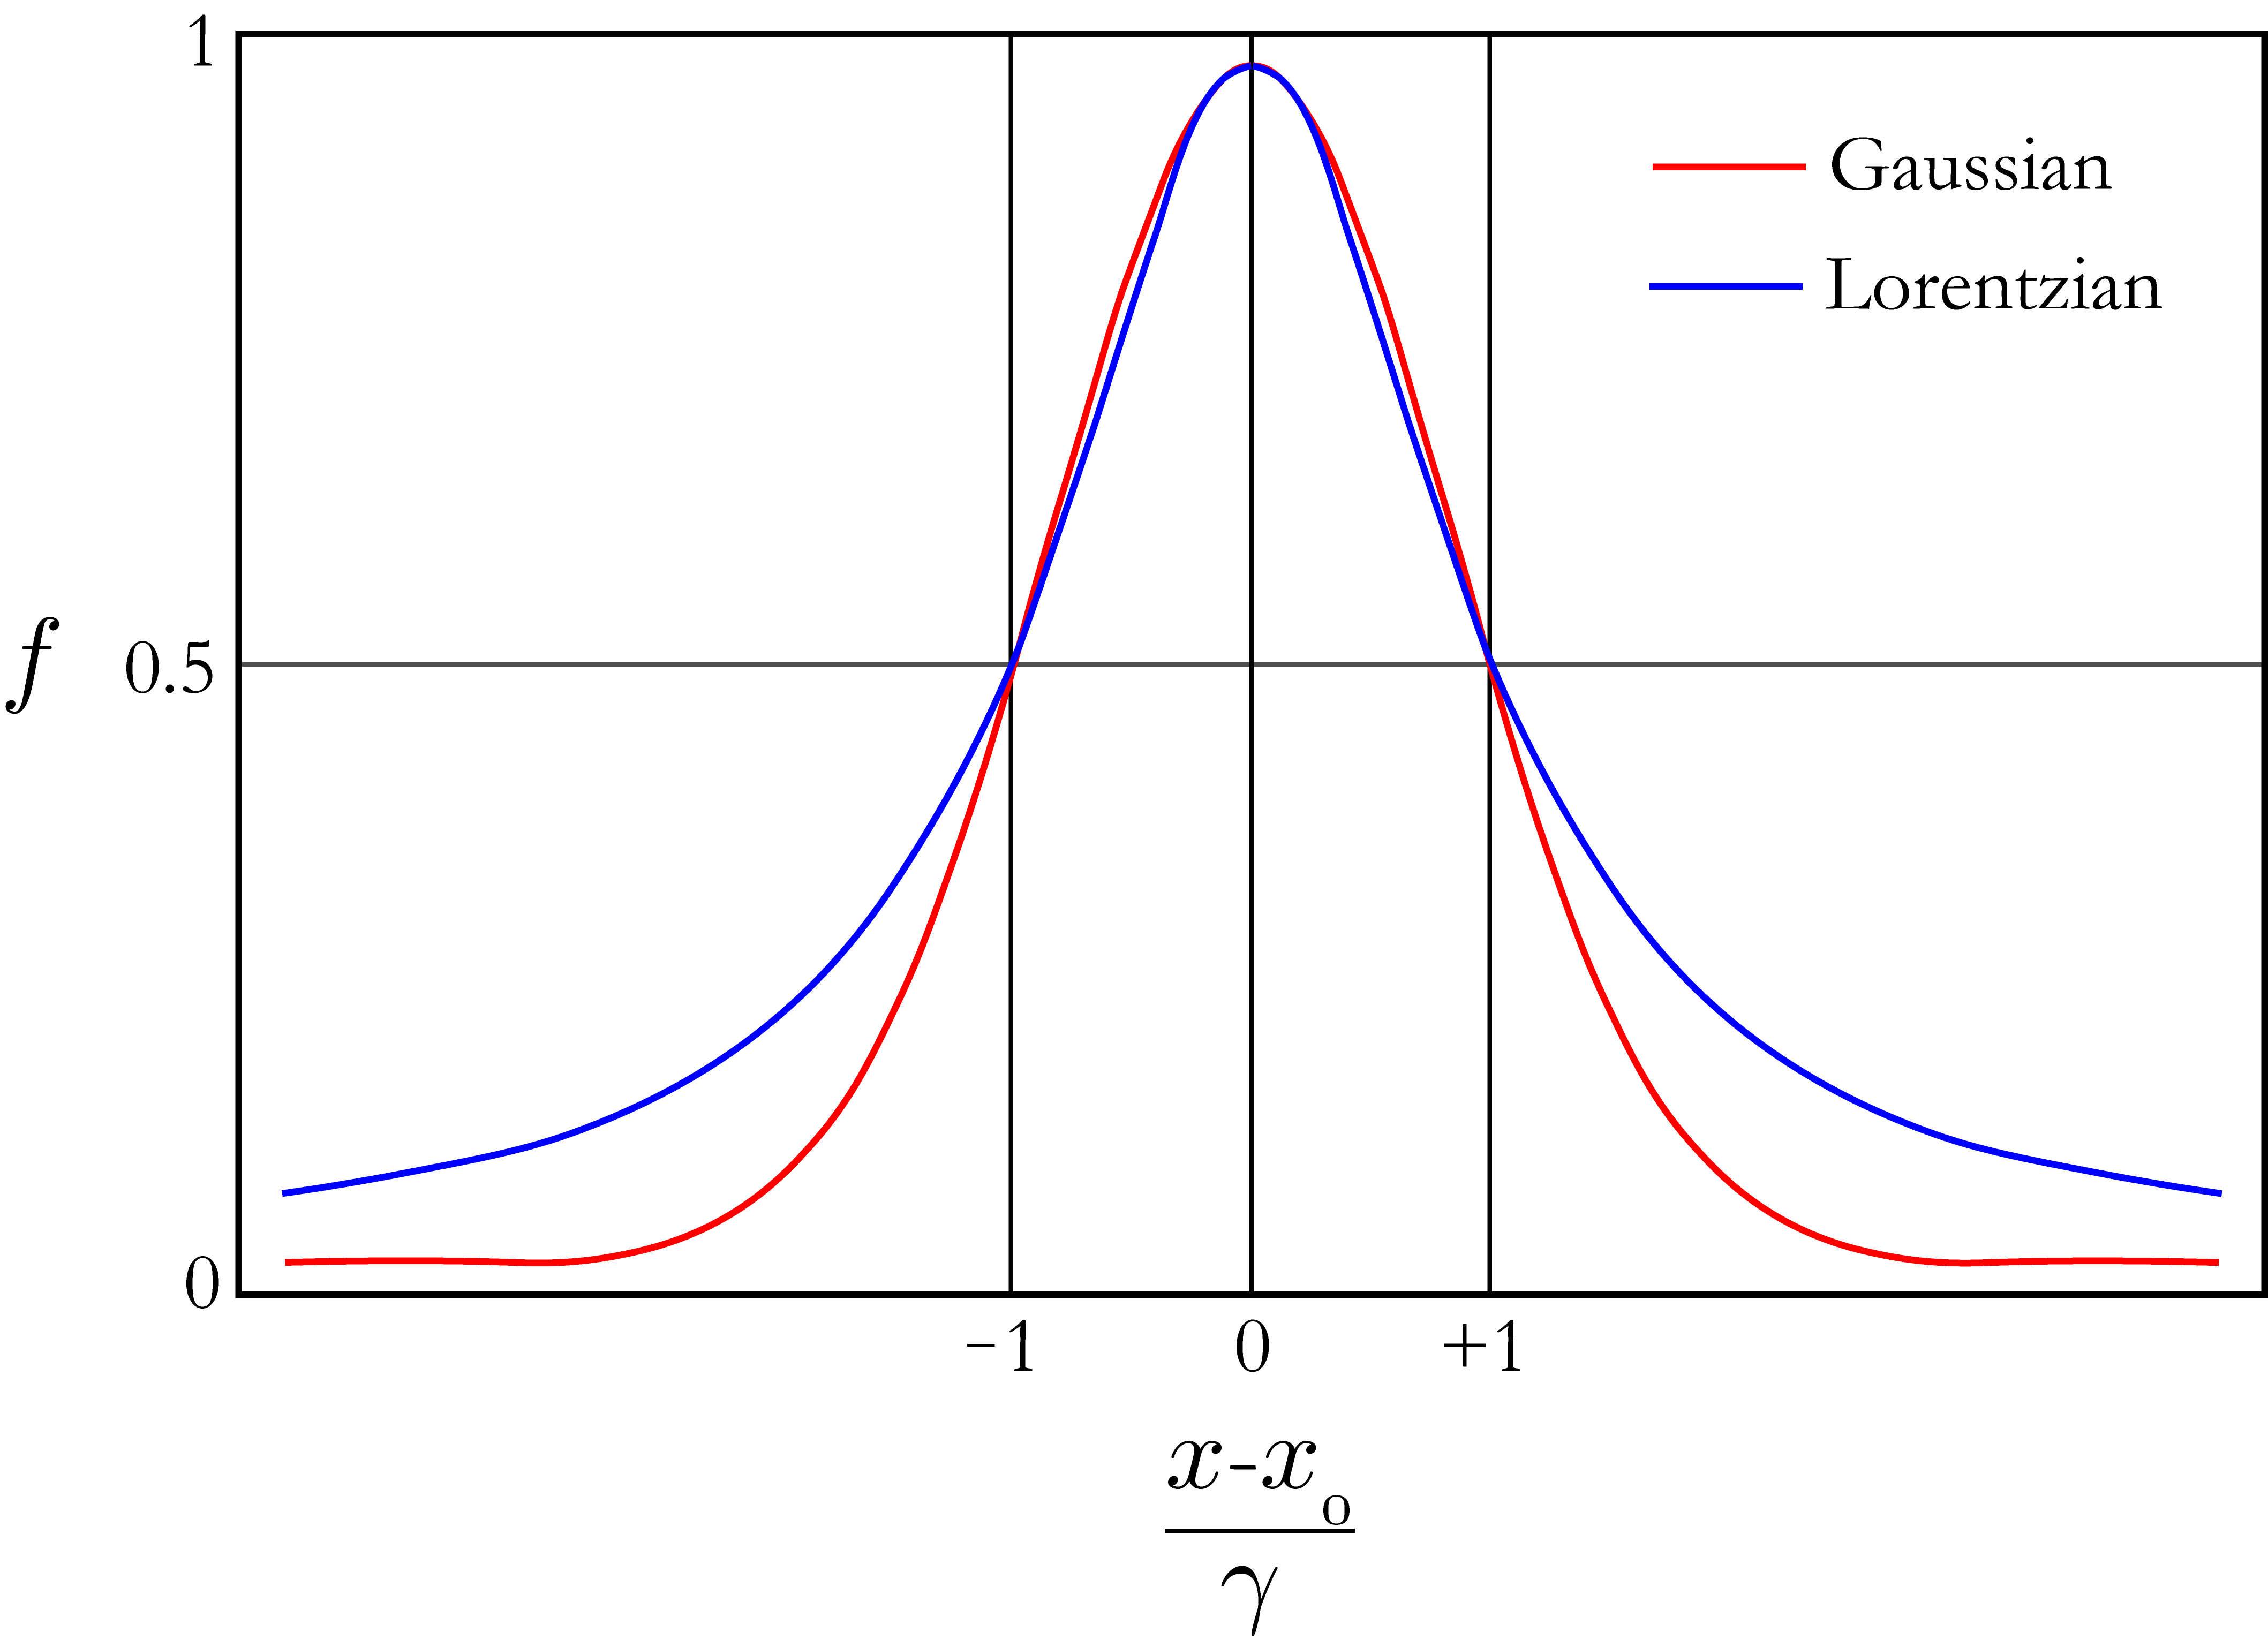
\includegraphics[width=10cm]{image/6-3-5.png}
\caption{高斯型和洛伦兹型\protect\footnotemark}

\end{figure}

\footnotetext{高斯型是指高斯分布:
\[{\rm pdf.}=\frac{1}{\sqrt{2\pi}\sigma}\ue^{-\frac{(x-x_0)^2}{2\sigma^2}}\]}

这样一个分布函数是需要有归一化的要求的:
\[\int_{-\infty}^{+\infty}{\rm pdf. }\,\ud x=1\]

但是现在的幅频特性,\,明显与洛伦兹型是有出入的.\,第一是,\,我们需要把因变量修改为$I=|A|^2$而不是$|A|$.\,这代表振动的强度而不是振幅.\,第二是,\,不同于柯西分布的分母为二次函数,\,这里的分母却作为了$x$的四次函数.\.也是$\omega$的四次函数.\,虽然$I(\omega)$与柯西分布有别,\,而且也不归一化.\,但是却体现出类似的性质.\,它们都是有一个峰,\,并在峰两侧按照较慢的多项式的方式衰减(而不是像高斯型那样指数衰减).\,而且我们都用\emph{半高峰宽}(FWHM,\,full width at half maximum)来描述峰的宽度.\,它被定义为函数值,\,或者代表的强度减少为峰值的一半对应的两点之间的区间宽度.\,对于标准的洛伦兹型,\,容易发现半高峰宽就是:
\[{\rm FWHM}=2\gamma\]

谐振子的幅频曲线的半高峰宽就更加难算.\,我们此时会采取一个近似技巧,\,不难验证其正确性.\,注意到在洛伦兹型中取到半高的点处分母中的两项是相等的,\,于是有理由相信在$I(x)$函数情况下,\,直接让分母两项相等就也近似是在半高点处:
\[I(x)=I_0\left/\middle[(1-x^2)^2+\frac{x^2}{Q^2}\right]\quad\Rightarrow\quad I_{\rm max}\approx I_0\]
\[I=\frac{I_{\rm max}}{2}\quad\Rightarrow\quad 1-x^2\approx \pm\frac{x}{Q}\]

这就可以确定,\,取到半高的点$x_+,\,x_-$为:
\[x_+=\sqrt{1+\frac{1}{4Q^2}}+\frac{1}{2Q}\quad;\quad x_-=\sqrt{1+\frac{1}{4Q^2}}-\frac{1}{2Q}\quad\Rightarrow \quad x_+-x_-=\frac{1}{Q}\]



而$\omega_+=x_+\omega_0,\,\omega_-=x_-\omega_0$.\,从而半高峰宽就是:
\[{\rm FWHM}=\Delta\omega=\omega_+-\omega_-=\frac{\omega_0}{Q}\]

我们又发现了品质因数的一种常见定义方式,\,它被定义为谱线的\emph{锐度}(sharpness),\,即峰处角频率与半高峰宽的比值:
\[Q=\frac{\omega_0}{\Delta \omega}\]





\section{多自由度小振动*}

多自由度小振动,\,首先得是一个多自由度平衡问题.\,在上一章带约束的完整系统的静力学平衡的基础上.\,如果体系还存在$f$个自由度,\,与之对应的有$f$个广义坐标$q_i$.\,那么我们指出过,\,体系的平衡条件为:
\[Q_i=\sum_k \bs{F}_k\cdot \frac{\partial \bs{r}_k}{\partial q_i}=0\]

但是在绝大多数情况下,\,我们处理的是保守体系的问题.\,所以这种场合下又有势能函数$V(q_i)$.\,广义力也能从势能中得到:
\[Q_i=\frac{\partial V}{\partial q_i}\]

这完全就能得到保守体系的平衡条件:
\[\frac{\partial V}{\partial q_i}=0\]

又是在绝大多数情况下,\,势能函数是性质非常良好的函数\footnote{数学上叫做光滑函数.}.\,从而可以在平衡位置附近泰勒展开.\,把平衡位置记作$q_{i0}$,\,而偏离平衡位置的位移为$\delta_i$,\,平衡位置处势能记作$V_0=V(q_{i0})$,\,由于平衡位置一阶导数为零,\,故:
\[V(q_{i0}+\delta_i)=V_0+\frac{1}{2}\sum_{i,\,j}\left.\frac{\partial^2 V}{\partial q_i\partial q_j}\right|_{q_{i0}}\delta_i\delta_j+\frac{1}{3!}\sum_{i,\,j,\,k}\left.\frac{\partial^3 V}{\partial q_i\partial q_j\partial q_k}\right|_{q_{i0}}\delta_i\delta_j\delta_k+\cdots\]

在忽略三阶小量(不会成为领头项,\,条件下面再讨论)的前提下,\,再通过去掉常数$V_0$,\,不影响势能的效果.\,我们发现势能实际上就成为了一个二次型:
\[V=\frac{1}{2}\sum_{i,\,j}\left.\frac{\partial^2 V}{\partial q_i\partial q_j}\right|_{q_{i0}}\delta_i\delta_j=\frac{1}{2}\sum_{i,\,j} V_{ij}\delta_i\delta_j\]

而动能,\,由于在平衡位置附近小范围内做小的运动,\,当然也是一个关于广义速度的二次型,\,系数为常数$T_{ij}$:
\[T=\frac{1}{2}\sum_{i,\,j} T_{ij}\dot{\delta}_i\dot{\delta}_j\]

关于系数$T_{ij},\,V_{ij}$.\,一个要求是它们必须对称:
\[T_{ij}=T_{ji}\quad;\quad V_{ij}=V_{ji}\]

其中的道理非常简单,\,例如只有两个广义坐标的变化$\delta_1,\,\delta_2$.\,那么$V_{12}=a\neq V_{21}=b$所决定的势能二次型与$V_{12}=V_{21}=(a+b)/2$决定的二次型根本就是同一个:
\[V_{12}=a\neq V_{21}=b:\,V=\frac{1}{2}V_{11} \delta_1^2+\frac{1}{2}V_{22} \delta_2^2+\frac{1}{2}a\delta_1\delta_2+\frac{1}{2}b\delta_2\delta_1=\frac{1}{2}V_{11} \delta_1^2+\frac{1}{2}V_{22} \delta_2^2+\frac{1}{2}(a+b)\delta_1\delta_2\]
\[V_{12}=V_{21}=\frac{a+b}{2}:\,V=\frac{1}{2}V_{11} \delta_1^2+\frac{1}{2}V_{22} \delta_2^2+\frac{1}{2}\frac{a+b}{2}\delta_1\delta_2+\frac{1}{2}\frac{a+b}{2}\delta_2\delta_1=\frac{1}{2}V_{11} \delta_1^2+\frac{1}{2}V_{22} \delta_2^2+\frac{1}{2}(a+b)\delta_1\delta_2\]

反过来,\,如果给一个二次型,\,我们也中总可以把系数写成对称的形式,\,比如在动能中,\,毕竟偏导数本身也是可交换次序的:
\[T_{ij}=\frac{\partial^2 T}{\partial \dot{\delta}_i\partial \dot{\delta}_j}=\frac{\partial^2 T}{\partial \dot{\delta}_j\partial \dot{\delta}_i}=T_{ji}\]

\begin{wrapfigure}[38]{o}[-10pt]{6cm}
\centering
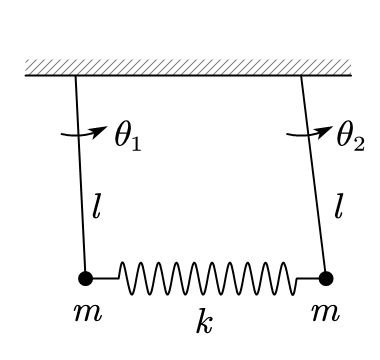
\includegraphics[width=6cm]{image/6-3-7.png}
\caption{耦合摆}\label{6-3-6}
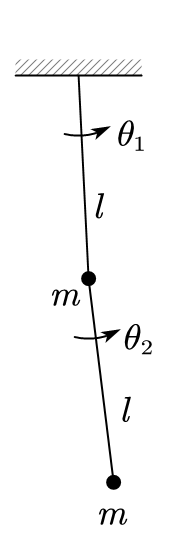
\includegraphics[width=2.5cm]{image/6-3-6.png}
\caption{双摆}\label{6-3-7}
\end{wrapfigure}
举两个例子.\,在\emph{耦合摆}(coupled pendulum)问题\ref{6-3-6}中,\,分开看是相同的两个单摆,\,但却因为弹簧而发生弱的耦合,\,设想弹簧原长为$x$为摆间距,\,这样就使得两单摆按原来的位置平衡时,\,弹簧也没有作用力.\,但只要一发生运动就彼此影响,\,设两摆球距离$x'=\sqrt{(x+l\sin\theta_2-l\sin\theta_1)^2+(l\cos\theta_2-l\cos\theta_1)^2}$.\,这样作为整体体系动能和势能为:
\[T_{\rm cp}=\frac{1}{2}ml^2\dot{\theta}_1^2+\frac{1}{2}ml^2\dot{\theta}_2^2\]
\[V_{\rm cp}=mgl(1-\cos\theta_1)+mgl(1-\cos\theta_2)+\frac{1}{2}k(x'-x)^2\]

再引入描述耦合强度的参量$\varepsilon=kl/mg$,\,小量近似以后,\,动能,\,势能被近似为二次型:
\[T_{\rm cp}=\frac{1}{2}\cdot ml^2\cdot \dot{\theta}_1^2+\frac{1}{2}\cdot ml^2\cdot \dot{\theta}_2^2\]
\[V_{\rm cp}=\frac{1}{2}\cdot (1+\varepsilon)mgl\cdot{\theta}_1^2+\frac{1}{2}\cdot (1+\varepsilon)mgl\cdot{\theta}_2^2-\varepsilon mgl\cdot {\theta}_1{\theta}_2\]

而在\emph{双摆}(double pendulum)问题\ref{6-3-7}中,\,两个摆直接悬挂在一起.\,也会彼此影响.\,体系动能和势能为:
\[T_{\rm dp}=\frac{1}{2}ml^2\dot{\theta}_1^2+\frac{1}{2}ml^2[\dot{\theta}_1^2+\dot{\theta}_2^2+2\dot{\theta}_1\dot{\theta}_2\cos(\theta_1-\theta_2)]\]
\[V_{\rm dp}=mgl(1-\cos\theta_1)+mgl(1-\cos\theta_1)+mgl(1-\cos\theta_2)\]


小量近似以后,\,动能,\,势能被近似为二次型:
\[T_{\rm dp}=\frac{1}{2}\cdot 2ml^2\cdot\dot{\theta}_1^2+\frac{1}{2}\cdot ml^2\cdot\dot{\theta}_2^2+ml^2\cdot\dot{\theta}_1\dot{\theta}_2\]
\[V_{\rm dp}=\frac{1}{2}\cdot 2mgl\cdot{\theta}_1^2+\frac{1}{2}\cdot mgl\cdot{\theta}_2^2\]

如果把$T_{ij}$和$V_{ij}$写成矩阵,\,那么对应的矩阵叫做\emph{惯性矩阵}(inertial matrix)和\emph{弹性矩阵}(elastic matrix):
\[[T_{ij}]_{\rm cp}=ml^2\begin{bmatrix} 1&0\\ 0&1\end{bmatrix}\quad;\quad [V_{ij}]_{\rm cp}=mgl \begin{bmatrix} 1+\varepsilon&-\varepsilon\\ -\varepsilon &1+\varepsilon\end{bmatrix}\]
\[[T_{ij}]_{\rm dp}=ml^2\begin{bmatrix} 2&1\\ 1&1\end{bmatrix}\quad;\quad [V_{ij}]_{\rm dp}=mgl \begin{bmatrix} 2&0\\ 0&1\end{bmatrix}\]

从而我们可以发现这两个问题的重大区别在于,\,前一个问题动能规整,\,势能却具有交叉项.\,后一个问题势能规整,\,动能却具有交叉项.

当我们遇到一个这样普遍的小振动问题时,\,该如何得到其运动的特征.\,有两种常见的做法:\,一是通过换元来实现动能势能的简化,\,这种方法需要较深厚的数学基础,\,又最好通过拉格朗日方程来理解一些过程.\,我们下面也写出具体的过程,\,有兴趣的读者可以做进一步研究;\,但也有第二种简易的方法来求解一些直接的量.\,我们也在详细讨论的方法之后加上去:

\subsection{基于线性代数与分析力学的简正坐标求解}

对一个任意的二次型进行配方并不是难事.\,例如$F(x_1,\,x_2\cdots)$是一个二次型,\,那么它必然可以写作:
\[F(x_1,\,x_2\cdots)=\frac{1}{2}f_{11}x_1^2+x_1(f_{12}x_2+f_{13}x_3+\cdots)+(\frac{1}{2}f_{22}x_2^2+\cdots)\]

即$x_1$自己的项,\,和别的变量``耦合''的项以及与$x_1$无关的项.\,那么做变量代换:
\[x_1'=x_1+\frac{f_{12}}{f_{11}}x_2+\frac{f_{13}}{f_{11}}x_3+\cdots\]

便可以把``耦合''项配方到$x_1$自己的项内,\,上式变成:
\[F(x_1,\,x_2\cdots)=\frac{1}{2}f_{11}x_1'^2+F'(x_2,\,x_3\cdots)\]

之后只要继续对$F'$配方,\,每次可以得到一个完全平方的项,\,余项则是剩下的变量的二次型,\,变量数至少减一.\,这样就可以实现任意二次型的完全配方.\,用这个方法可以选择动能或者势能进行化简.\,最终形式,\,由上讨论,\,只包含平方项,\,没有交叉项.\,由于这样对应的矩阵是对角矩阵.\,我们把这样的配方过程称作\emph{对角化}(diagonalization):
\[T=\sum_i\frac{1}{2}T_i \dot{\delta}_i^2\quad ;\quad V=\sum_i\frac{1}{2}V_i \delta_i^2\]

注意这里动能和势能的对角化是分开来进行的.\,对应的系数$T_i$叫做\emph{惯性系数}(inertial coefficient),\,而$T_i$叫做\emph{弹性系数}(elastic coefficient).\,同时我们对这些系数必然有以下期待:

\begin{itemize}
	\item 动能的对角化结果:
		\begin{itemize}
			\item 非退化正定二次型:\,所有$T_i>0$.
			\item 退化正定二次型:\,个别$T_i=0$.
			\item 不可能出现某个$T_i<0$.
		\end{itemize}
	\item 势能的对角化结果:
		\begin{itemize}
			\item 非退化正定二次型:\,所有$V_i>0$.
			\item 可以负的二次型:\,存在$V_i<0$.
			\item 退化的二次型:\,所有$V_i\geq 0$且也存在$V_i= 0$.
		\end{itemize}
\end{itemize}

说明:

动能不可以出现负的惯性系数,\,是因为在所有情况下动能都必须大于零.\,但是在有的情况下惯性系数可以为零,\,即,\,即使广义速度不为零,\,造成的动能为零,\,称作\emph{退化}(degenarate)的情况.\,这要么说明体系存在没有动力学效果的冗余自由度.\,例如无限细的杆的自转角就是这样的例子.\,去掉这个广义坐标也不影响能量的表达式.\,要么说明这个自由度上的动能是一个高阶小量.\,只是在目前平衡位置,\,系数``偶然''地等于了零,\,只要偏离这个位置去振动就会产生一定的动能,\,抑或我们在实际问题中需要考虑更高阶泰勒展开产生的广义速度的高次项.\,后面这种情况一般就与简谐振动无关了.\,再次不予考虑.\,故我们此后做假设:\,\emph{所有小振动问题,\,动能必须是非退化正定的.}

势能就更加复杂.\,势能相对平衡位置本来就可正可负.\,那么上面我们分为三种情况其实就包括了所有情况.\,有一点是非常突出的,\,如果沿某方向偏离平衡位置时,\,势能降低了,\,那么原平衡位置就一定是\emph{非稳定平衡}(unstable equilibrium).\,在仅仅考虑二次型的情况下,\,一旦出现一个负的弹性系数这就成为了必然.\,但是即使一个负的弹性系数都没有,\,也不能因此就下断言原位置是稳定的.\,因为还有二次型\emph{退化}的情况.\,它发生在某些弹性系数为零时,\,此时高阶泰勒展开项如果是负的,\,它依然可以不稳定,\,普遍情况得考察多个领头项.\,但是,\,有一点很好判断:\,就是如果所有弹性系数为正,\,那么原来的位置就一定是\emph{稳定平衡}(stable equilibrium).\,因为此时任意的偏离平衡位置都使得势能升高.\,也只有稳定平衡才能作为小振动问题求解的先决条件.\,故我们此后做假设:\,\emph{所有小振动问题,\,势能必须是非退化正定的.}

但是虽然单独对动能或势能对角化简单,\,但是两者却不会同时对角化.\,例如在双摆问题中,\,对于动能:
\[T_{\rm dp}=\frac{1}{2}\cdot 2ml^2\cdot\dot{\theta}_1^2+\frac{1}{2}\cdot ml^2\cdot\dot{\theta}_2^2+ml^2\cdot\dot{\theta}_1\dot{\theta}_2=\frac{1}{2}\cdot 2ml^2\cdot\left(\dot{\theta}_1+\frac{1}{2}\dot{\theta}_2\right)^2+\frac{1}{2}\cdot \frac{ml^2}{2}\cdot\dot{\theta}_2^2\]

但是如果做换元$\vartheta_1=\theta_1+\theta_2/2,\,\vartheta_2=\theta_2$,\,动能倒是没有交叉项了,\,但原来好好的势能又产生交叉项了:
\[V_{\rm dp}=\frac{1}{2}\cdot 2mgl\cdot{\vartheta}_1^2+\frac{1}{2}\cdot \frac{3}{2}mgl\cdot{\vartheta}_2^2-mgl\cdot {\vartheta}_1{\vartheta}_2\]

所以,\,我们这里要追求的其实是\emph{同时对角化}(simutalneous diagonalization)的技巧.\,为了进一步研究,\,我们先来抽象对角化的过程.\,根据矩阵理论,\,任何一个坐标变换,\,其实是一个线性变换:
\[[q_i']=[A_{ij}][q_j]\]

这个式子是以下两种写法的缩略形式:
\[q_i'=\sum_j A_{ij}q_j\quad {\rm or}\quad \begin{bmatrix}q_1'\\q_2'\\ \vdots\\ q_n'\end{bmatrix}=\begin{bmatrix}A_{11}&A_{12}&\cdots&A_{1n}\\ A_{21}&A_{22}&\cdots &A_{2n}\\ \vdots&\vdots &&\vdots\\ A_{n1}&A_{n2}&\cdots &A_{nn} \end{bmatrix}\begin{bmatrix}q_1\\q_2\\ \vdots\\ q_n\end{bmatrix}\]

它的逆变换:\,求出$[A_{ij}]$的逆矩阵$[B]_{ij}$,\,就可以用新坐标表示旧坐标:
\[[q_i]=[B_{ij}][q_j']\]

而动能,\,势能都可以用矩阵来表示\footnote{用$\phantom{}^{\rm t}[q_i]$表示转置,\,即把列向量写作行向量.}:
\[T=\frac{1}{2}\phantom{}^{\rm t}[\dot{q}_i][T_{ij}][\dot{q}_j]\quad ;\quad V=\frac{1}{2}\phantom{}^{\rm t}[q_i][V_{ij}][q_j]\]

这样只要把之前的变换代入这两个二次型,\,就得到了变换之后的二次型:
\[T=\frac{1}{2}\phantom{}^{\rm t}[\dot{q}'_i]\phantom{}^{\rm t}[B_{ij}][T_{jk}][B_{kl}][\dot{q}'_l]=\frac{1}{2}\phantom{}^{\rm t}[\dot{q}'_i][T'_{il}][\dot{q}'_l]\]
\[V=\frac{1}{2}\phantom{}^{\rm t}[q'_i]\phantom{}^{\rm t}[B_{ij}][V_{jk}][B_{kl}][q'_l]=\frac{1}{2}\phantom{}^{\rm t}[q'_i][V'_{il}][q'_l]\]

这说明其实在坐标变换以后,\,惯性和弹性矩阵是按照右乘一个矩阵,\,再左乘它的转置来进行的.\,这种对矩阵的变换数学上叫做\emph{合同变换}(congruent transformation):
\[[T'_{il}]=\phantom{}^{\rm t}[B_{ij}][T_{jk}][B_{kl}]\quad ;\quad [V'_{il}] =\phantom{}^{\rm t}[B_{ij}][V_{jk}][B_{kl}]\]

要把$[T]$和[V]同时对角化,\,其实问题的诀窍是求解\emph{本征值问题}(eigenvalue problem):
\[([V_{ij}]+\lambda [T_{ij}])[x_j]=[0]\]

即,\,确定是否存在常数$\lambda$\footnote{后面会知道一定非零.}和非零向量$[x_j]$使得两个矩阵组合以后恰好作为系数使得这个向量作为以上方程的解.\,乍一看这似乎很抽象.\,其实这背后的物理意义可以做这样的理解:\,既然是小振动,\,就有可能找到一些简单的运动模式,\,此时所有坐标上都是做不同振幅的简谐振动,\,即:
\[[q_i]=[x_i]\cos\omega t\]




如何写出这种情况下的动力学方程?\,一种完全严谨的做法就是利用上一章讨论的拉格朗日方程:
\[L=T-V=\frac{1}{2}\phantom{}^{\rm t}[\dot{q}_i][T_{ij}][\dot{q}_j]-\frac{1}{2}\phantom{}^{\rm t}[q_i][V_{ij}][q_j]\]

\[\frac{\ud }{\ud t}\frac{\partial L}{\partial \dot{q}_i}=\frac{\partial L}{\partial {q}_i}\quad\Rightarrow \quad [T_{ij}][\ddot{q}_j]=-[V_{ij}][q_j]\]

将简谐振动解带入,\,就得到了:
\[([V_{ij}]-\omega^2 [T_{ij}])[x_j]=[0]\]

从而原来的本征值问题中的$\lambda$代表的含义就是振动角频率平方$\omega^2$.\,那么这个本征值问题又如何求解?\,首先,\,上式中方程组存在解且非零的条件为系数行列式为零:
\[{\rm det}([V_{ij}]-\lambda [T_{ij}])=0\]

这就构成了关于$\lambda$的$n$次方程,\,他就一定有$n$个根,\,不过可以有重根.\,把这$n$个根带入,\,我们就可以把对应的$n$个本征向量\footnote{注意本征向量的存在性,\,非重根是显然的,\,但是如果有个$s$重根,\,是否也有$s$组独立的解向量?\,这不是显然的,\,需要证明,\,在次略去.\,一般线性代数的教材上都会有证明方法,\,不过一般会默认是$[T_{ij}]$为单位矩阵的简单情况,\,其实这不影响证明过程.}$[x_j]$找到,\,这仅仅是个体力活:\,求解至多$n$次$n$元线性方程组.\,一旦求解完毕,\,我们就找到了$n$个$\lambda$和$n$个$[x_j]$,\,可以记作:
\[([V_{ij}]-\lambda_k [T_{ij}])[B_{j,k}]=[0]\]

最后还需证明一点,\,就是这$k=1,\,2\cdots n$个本征值对应的本征向量不仅是独立的,\,而且还是\emph{正交}(orthogonal)的.\,注意这里的正交是指:
\[k\neq k'\quad\Rightarrow\quad\phantom{}^{\rm t}[B_{i,k}][T_{ij}][B_{j,k'}]=0\]

这个正交性足以说明独立性,\,毕竟如果$[B_{i,k}]$与$[B_{i,k'}]=0$不独立,\,那么前者(非零)就是后者(非零)的常数(非零)倍,\,以上$\phantom{}^{\rm t}[B_{i,k}][T_{ij}][B_{j,k'}]$就会变成常数乘以后者产生的动能,\,显然是非零的.\,所以一旦上式为零,\,两个矢量正交就足以说明它们不会同向.

证明正交性的依据还是它们的定义.\,首先我们发现,\,如果任意两个矢量恰好成为不同本征值下的本征向量:
\[([V_{ij}]-\lambda_1 [T_{ij}])[x_{j,1}]=[0]\;,\;([V_{ij}]-\lambda_2 [T_{ij}])[x_{j,2}]=[0]\quad,\quad \lambda_1\neq\lambda_2\]

构造式子$\phantom{}^{\rm t}[x_{i,1}][V_{ij}][x_{j,2}]$.\,一方面先计算前面的向量乘弹性矩阵,\,一方面也可以先算后面的向量乘弹性矩阵:
\[\phantom{}^{\rm t}[x_{i,1}][V_{ij}]=\lambda_1\phantom{}^{\rm t}[x_{i,1}][T_{ij}]\quad,\quad [V_{ij}][x_{j,2}]=\lambda_2[T_{ij}][x_{j,2}]\]
\[\Rightarrow \quad \phantom{}^{\rm t}[x_{i,1}][V_{ij}][x_{j,2}]=\lambda_1\phantom{}^{\rm t}[x_{i,1}][T_{ij}][x_{j,2}]=\lambda_2\phantom{}^{\rm t}[x_{i,1}][T_{ij}][x_{j,2}]\]
\[\lambda_1\neq \lambda_2 \quad\Rightarrow\quad [x_{i,1}][T_{ij}][x_{j,2}]=0\]

这实际上是证明了,\,由$n$个本征向量$[B_{i,k}]$形成的空间根据不同的本征值彼此正交,\,即使在某个本征值下有多个本征向量,\,总可以在它们线性组合形成的空间中选取相互正交的向量作为本征向量.\,这样我们就得到了一组特殊的本征向量,\,它们符合:
\[\phantom{}^{\rm t}[B_{i,k}][T_{ij}][B_{j,k'}]=0\quad{\rm if}\quad k\neq k'\]

而当$k=k'$时上述值一定大于零,\,这些结果,\,后面就可以看到,\,其实就是惯性系数:
\[\phantom{}^{\rm t}[B_{i,k}][T_{ij}][B_{j,k}]=T_k\]

现在我们直接把这$n$个$n$行的列向量横向按顺序并置构成矩阵:
\[[B_{ij}]=[[B_{i,\,1}]\,,\,[B_{i,\,2}]\cdots [B_{i,\,n}]]\]

这样以上关系其实就表示为了:
\[\phantom{}^{\rm t}[B_{ij}][T_{jk}][B_{kl}]=\mathfrak{Diag}(T_i)\]

其中$\mathfrak{Diag}(T_i)$表示由$T_i$作为元素的对角矩阵.\,同理我们如果考察弹性矩阵,\,也有:
\[\phantom{}^{\rm t}[B_{i,k}][V_{ij}][B_{j,k'}]=0\quad{\rm if}\quad k\neq k'\]
\[\phantom{}^{\rm t}[B_{i,k}][V_{ij}][B_{j,k}]=\lambda_k T_k=\omega_k^2T_k=V_k\]

同理用矩阵表示:
\[\phantom{}^{\rm t}[B_{ij}][V_{jk}][B_{kl}]=\mathfrak{Diag}(V_i)\]

这样我们之前的愿望就实现了,\,即动能矩阵与势能矩阵的同时对角化.

\vspace{1cm}

让我们来对双摆体系利用上述套路来求解:\,首先是对应的本征值问题的系数行列式为零:
\[[V]_{ij}=mgl\begin{bmatrix}2&0\\0&1\end{bmatrix}\quad;\quad [T]_{ij}=ml^2\begin{bmatrix}2&1\\1&1\end{bmatrix}\]
\[{\rm det}([V_{ij}]-\lambda [T_{ij}])=0\quad\Rightarrow\quad {\rm det}\begin{bmatrix}2g/l -2\lambda &-\lambda \\-\lambda&g/l -\lambda \end{bmatrix}=0\]
\[\Rightarrow\quad 2(g/l-\lambda)^2=\lambda^2\]

从而得到特征值:
\[\lambda_1=\omega_1^2=(2-\sqrt{2})\frac{g}{l}\quad;\quad\lambda_2=\omega_2^2=(2+\sqrt{2})\frac{g}{l}\]

带入本征值问题,\,分两个本征值来求解本征向量:
\[([V_{ij}]-\lambda_k [T_{ij}])[B_{j,k}]=0\;,\;k=1,\,2\]
\[\begin{bmatrix}2(\sqrt{2}-1)&-(2-\sqrt{2})\\-(2-\sqrt{2})&\sqrt{2}-1\end{bmatrix}\begin{bmatrix}B_{11}\\B_{21}\end{bmatrix}=\begin{bmatrix}0\\0\end{bmatrix}  \quad,\quad  \begin{bmatrix}-2(\sqrt{2}+1)&-(2+\sqrt{2})\\-(2+\sqrt{2})&-(\sqrt{2}+1)\end{bmatrix}\begin{bmatrix}B_{12}\\B_{22}\end{bmatrix}=\begin{bmatrix}0\\0\end{bmatrix}\]
\[\Rightarrow \quad \begin{bmatrix}B_{11}\\B_{21}\end{bmatrix}=\begin{bmatrix}1\\\sqrt{2}\end{bmatrix}\quad,\quad \begin{bmatrix}B_{12}\\B_{22}\end{bmatrix}=\begin{bmatrix}1\\-\sqrt{2}\end{bmatrix}\]

这就给出了一个坐标变换矩阵:
\[[B_{ij}]=\begin{bmatrix}1&1\\\sqrt{2}&-\sqrt{2}\end{bmatrix}\]

其逆矩阵:
\[[A_{ij}]=\begin{bmatrix}\frac{1}{2}&\frac{\sqrt{2}}{4}\\\frac{1}{2}&-\frac{\sqrt{2}}{4}\end{bmatrix}\]

这就是给出了如下的坐标变换:
\[\left\{\begin{array}{l}\varphi_1=\frac{1}{2}\theta_1+\frac{\sqrt{2}}{4}\theta_2\\ \varphi_2=\frac{1}{2}\theta_1-\frac{\sqrt{2}}{4}\theta_2\end{array}\right.\quad,\quad \left\{\begin{array}{l}\theta_1=\varphi_1+\varphi_2\\ \theta_2=\sqrt{2}\varphi_1-\sqrt{2}\varphi_2\end{array}\right.\]

代入便知,\,初始的动能和势能分别变为:
\[T=\frac{1}{2}\cdot 2ml^2\cdot\dot{\theta}_1^2+\frac{1}{2}\cdot ml^2\cdot\dot{\theta}_2^2+ml^2\cdot\dot{\theta}_1\dot{\theta}_2 \quad,\quad V=\frac{1}{2}\cdot 2mgl\cdot{\theta}_1^2+\frac{1}{2}\cdot mgl\cdot{\theta}_2^2\]
\[\Rightarrow \quad T=\frac{1}{2}\cdot 2(2+\sqrt{2})ml^2\cdot \dot{\varphi}_1^2+\frac{1}{2}\cdot 2(2-\sqrt{2})ml^2\cdot \dot{\varphi}_2^2\quad,\quad V=\frac{1}{2}\cdot 4mgl\cdot \varphi_1^2+\frac{1}{2}\cdot 4mgl\cdot \varphi_2^2\]

这就可以看作两个独立的振子,\,完成了\emph{解耦}(decouple).\,各自的角频率为:
\[\omega_1=\sqrt{\frac{4mgl}{2(2+\sqrt{2})ml^2}}\quad,\quad \omega_2=\sqrt{\frac{4mgl}{2(2-\sqrt{2})ml^2}}\]

与之前本征值确定的角频率是一样的.

现在我们来对这个结果产生的物理意义进行解释.\,通过坐标变换,\,我们发现动能势能形式变得简单了,\,所以新的坐标$q_i'$称作\emph{简正坐标}(normal coordinates).\,对应的频率$\omega_i$称作\emph{简正频率}(normal frequencies):
\[\omega_i=\sqrt\frac{V_i}{T_i}\quad {\rm or}\quad V_i=T_i\omega_i^2 \]

于是我们产生了一个疑问,\,为什么只要动能势能的形式变得简单,\,就可以判定体系可以等效为独立的谐振子的组合?\,其实它简单地来自于拉格朗日方程:
\[L=T-V=\sum_i\frac{1}{2}T_i(\dot{q}_i'^2-\omega_i^2q_i'^2)\]
\[\frac{\ud }{\ud t}\frac{\partial L}{\partial \dot{q}_i'}=\frac{\partial L}{\partial {q}_i'}\quad \Rightarrow \quad \ddot{q}'_i=-\omega_i^2q_i'\]

这就足以给出其解为简谐振动:
\[q_i'=C_i\cos(\omega_i t+\varphi_i)\]

再回到体系的初始广义坐标,\,它就会等于这些各自做不同频率振动的简正坐标的组合,\,从而体现出非常复杂的非简谐运动特性\footnote{要知道傅里叶理论可以证明,\,用不同频率的简谐振动组合可以无限接近任意光滑函数.}.\,具体各个广义坐标的振幅和初相位如何,\,由体系的初始条件决定.\,但是可以想象,\,存在一些简单的振动模式,\,它的初始条件决定了,\,最后只有一个简正坐标$q_k'$在做振动,\,其他的坐标振幅为零.\,那么最后原来的坐标也会具有单一的频率$\omega_k$,\,从而每一处运动都是简谐振动,\,其实它们为:
\[[q_i]=[B_{ij}][q_j']=[B_{i,\,k}]\cdot C_k\cos(\omega_k t+\varphi_k)\]

所以我们把体系以统一的频率,\,所有地方都做简谐振动的这种振动模式称作\emph{简正模}(normal mode).\,``简正''这个词语三次出现在相关术语中,\,它可以浅显地被理解为``简单''+``正确''.\,也可以更精确地被理解为``简谐''+``正交''.\,毕竟在中文语境下,\,简谐本意就是``简单''+``和谐'',\,而``正确''的``正''本身也含有方向的意味.\,英文语境下的``normal''也恰好有着异曲同工之妙.

\subsection{基于对称性的简正模判定与简正频率求解}

如何规避掉较难的数学和分析力学知识?\,用简单而优雅的方式快速确定一个多自由度简谐振动的绝大多数特征?\,我们可以采用与对称性结合的方式来求解其运动的微分方程.

就比如对于具有更好的对称性的耦合摆问题.\,我们不去追求用能量函数来解决问题,\,这样势必涉及到分析力学方法.\,而是独立地去推导两个质点的牛顿定律.\,很容易给出它们为:
\[\left\{\begin{array}{l}\ddot{\theta}_1=-\omega_0^2(1+\varepsilon)\theta_1+\omega_0^2\varepsilon\theta_2 \\ \ddot{\theta}_2=+\omega_0^2\varepsilon\theta_1-\omega_0^2(1+\varepsilon)\theta_2\end{array}\right.\]

其中$\omega_0=\sqrt{g/l}$.\,至于这个方程的求解,\,猜一个本征模解是常规操作:
\[\left\{\begin{array}{l} \theta_1=A_1\ue^{\ui\omega t}\\\theta_2=A_2\ue^{\ui\omega t} \end{array}\right.\]

但是在猜解之后,\,我们不一定要通过带入原方程,\,命系数行列式为零,\,再次带入本征频率来求解方程的曲折方程来求解振幅$A_1$和$A_2$的比.\,在本题中有一点是显然的.\,就是体系具有鲜明的左右对称性.\,这使得我们猜想:\,是不是在一种本征模式下,\,左右两个物体的位移完全相等.\,而另一个模式下,\,两个物体的位移完全相反?

这的确发生了.\,在经典物理情况下,\,这其实就对应了质心的左右振动和相对质心的二体在弹性内力下的振动.\,一般把两个物体位移相等的模式称作\emph{对称模式}(symmetric mode),\,而位移相反的模式称作\emph{反对称模式}(antisymmetric mode).\,即:
\[\left\{\begin{array}{l} \theta_{1S}=A\ue^{\ui\omega_S t}\\\theta_{2S}=A\ue^{\ui\omega_S t} \end{array}\right.\quad ,\quad \left\{\begin{array}{l} \theta_{1A}=A\ue^{\ui\omega_A t}\\\theta_{2A}=-A\ue^{\ui\omega_A t} \end{array}\right.\]

代入原来的方程就可以看出来:\,对称模式给出了:
\[-\omega_S^2A=-\omega_0^2(1+\varepsilon)A+\omega_0^2\varepsilon A\quad \Rightarrow \quad \omega_S=\omega_0\]
\[-\omega_A^2A=-\omega_0^2(1+\varepsilon)A-\omega_0^2\varepsilon A\quad \Rightarrow \quad \omega_A=\omega_0\sqrt{1+2\varepsilon}\]

可以发现,\,问题的关键在于如何看出振动模式下各个振幅之间的比例关系.\,这个问题似乎取决于问题具体的对称性.\,那么,\,何谓对称性?\,它又是怎样决定体系的振动解的.\,我们对一个更复杂的问题来做进一步研究:

\begin{figure}[H]
\centering
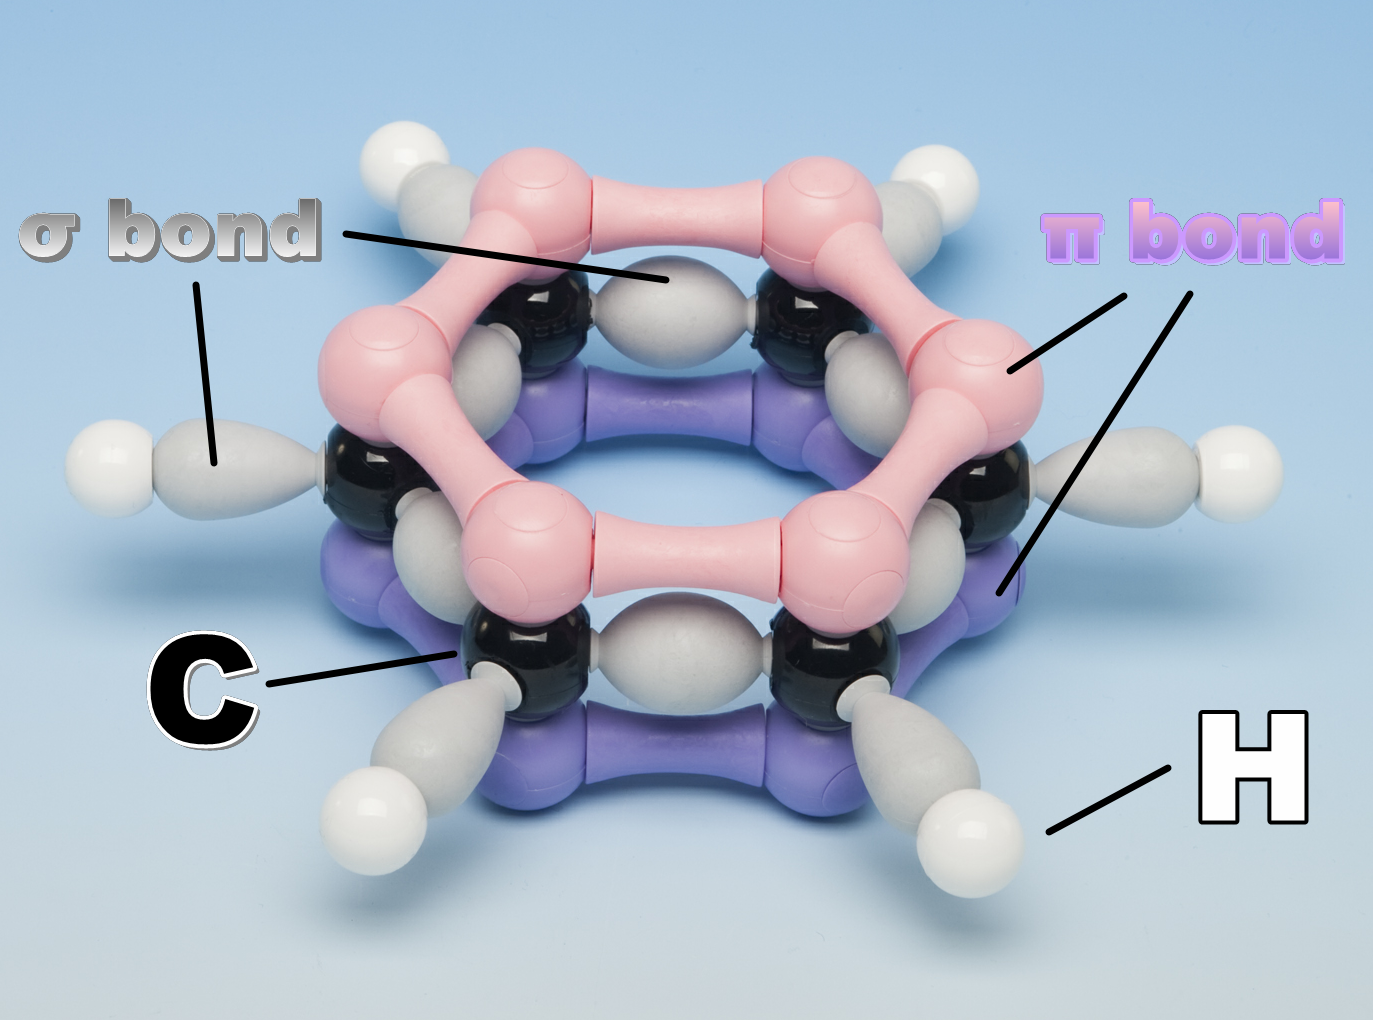
\includegraphics[width=7cm]{image/6-3-10.png}
\hspace{2cm}
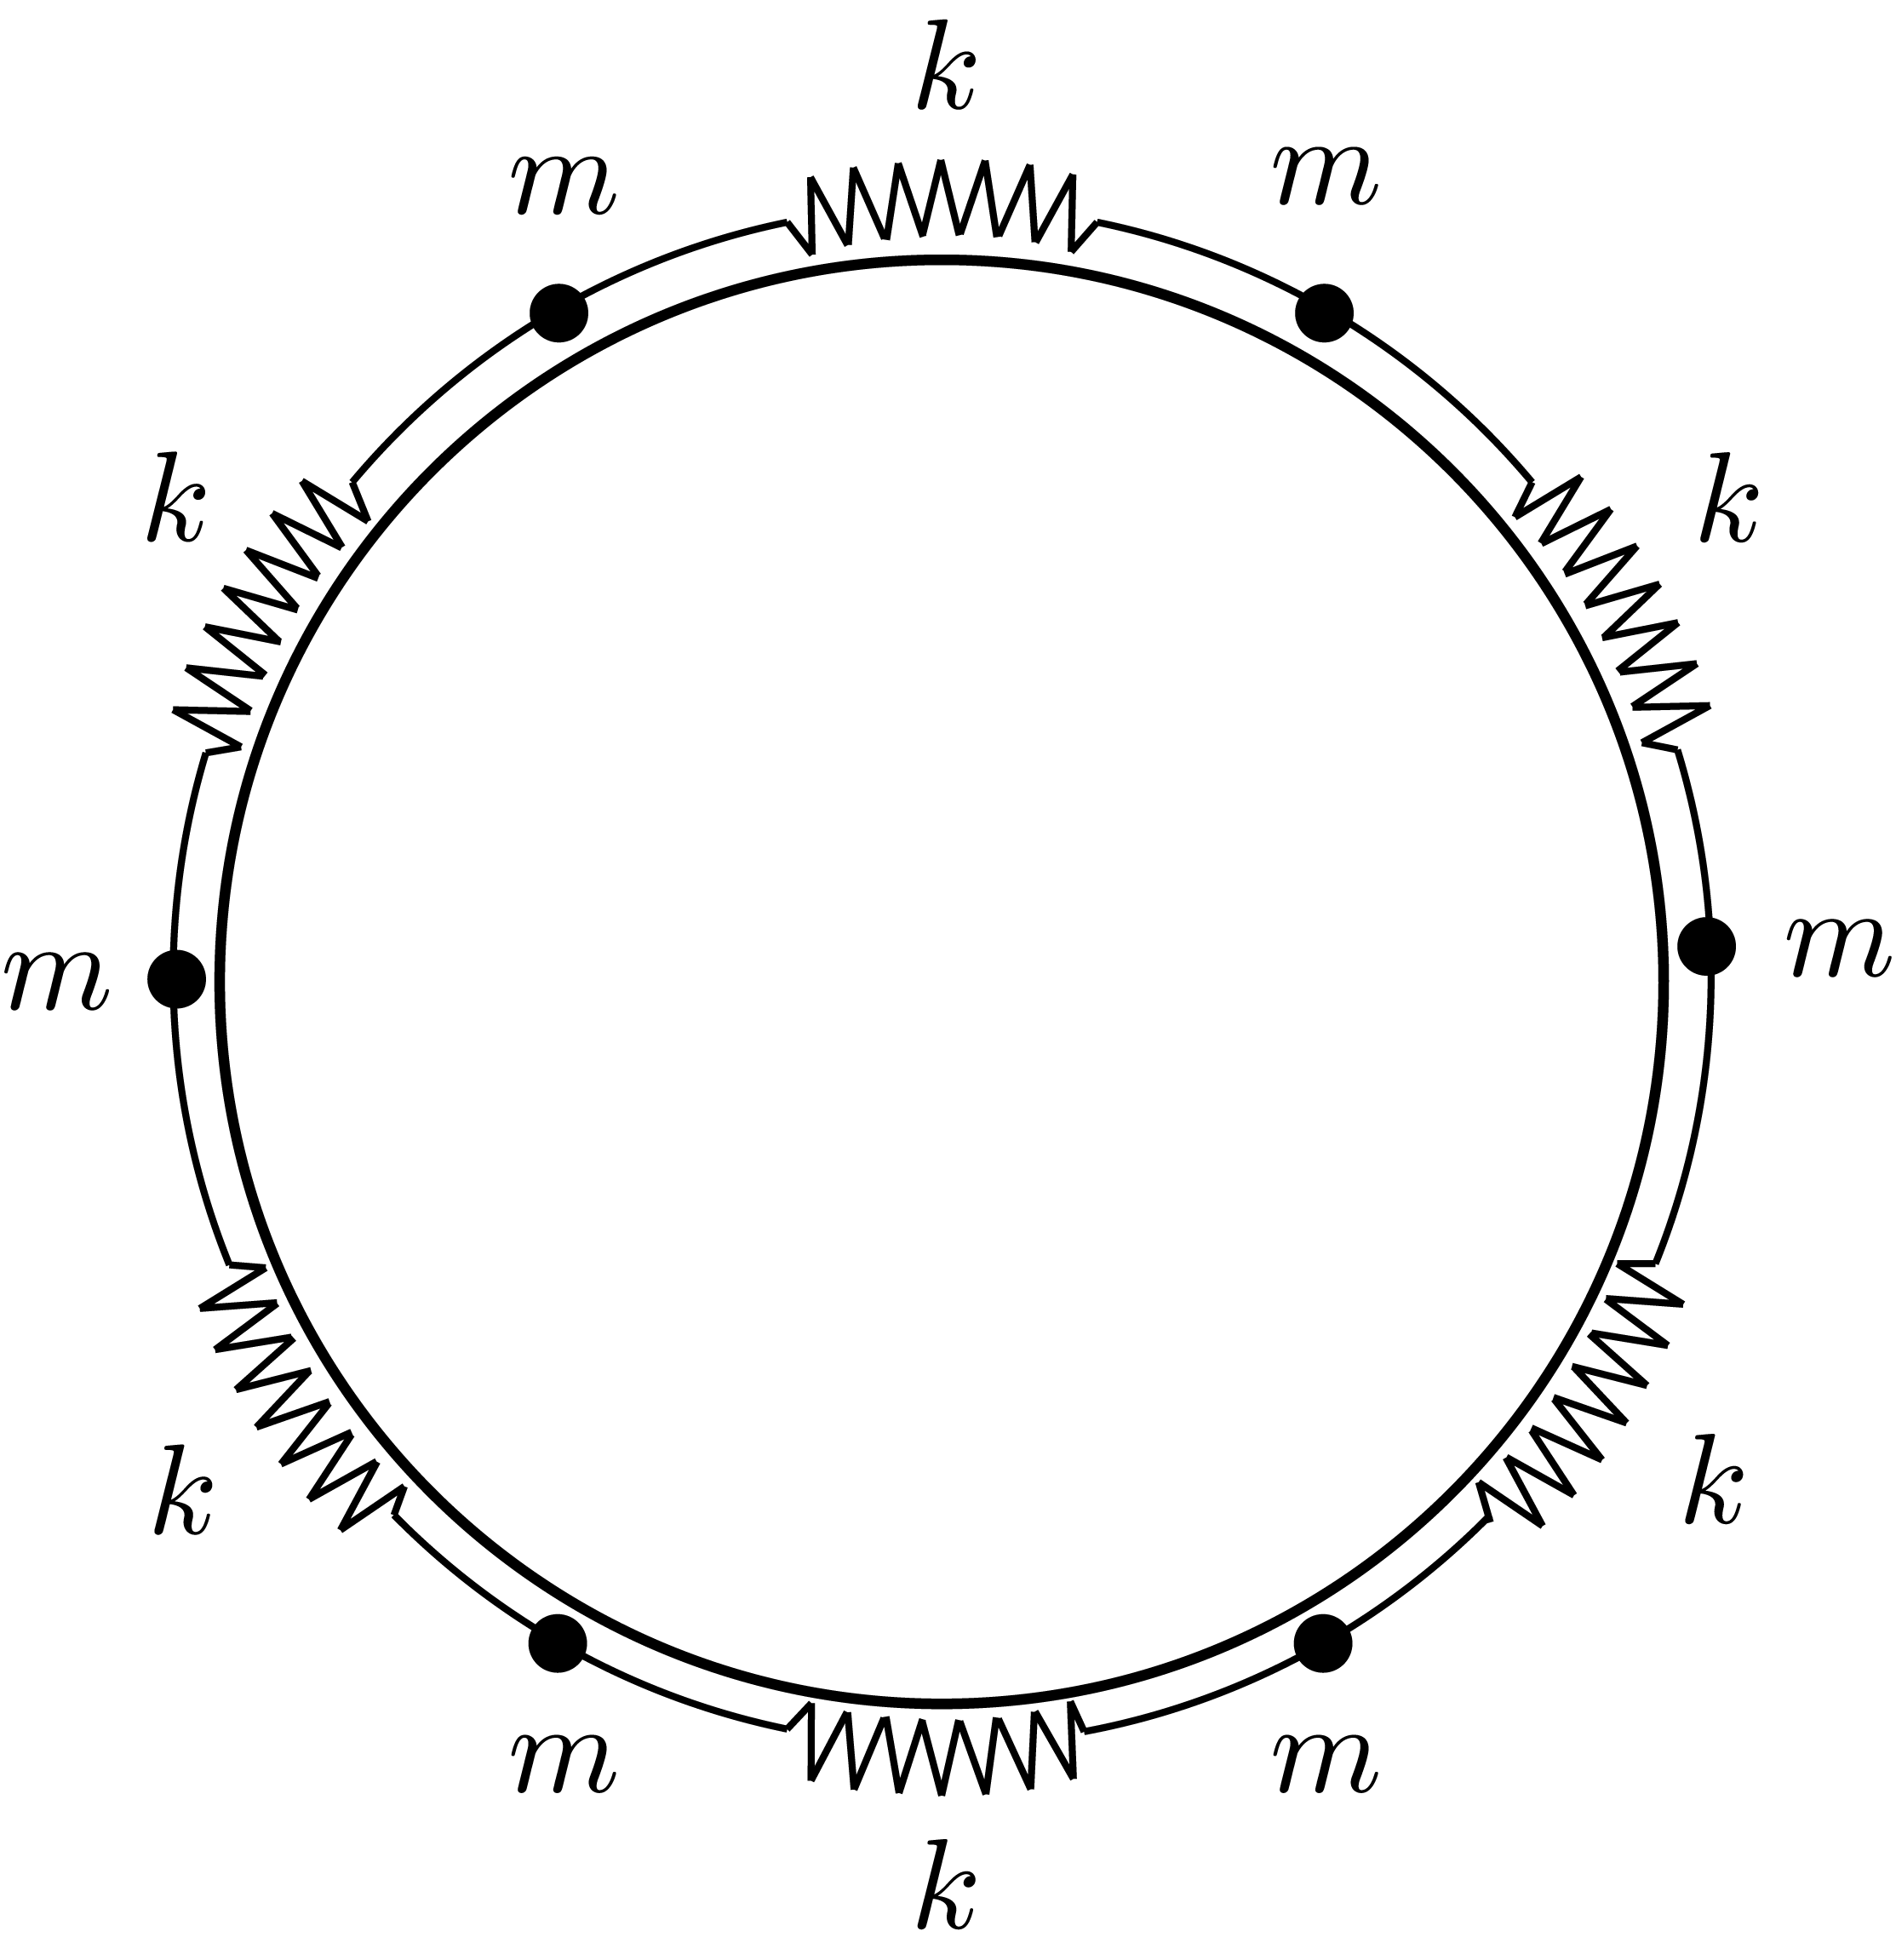
\includegraphics[width=5cm]{image/6-3-8.png}
\caption{苯: 6原子环问题}
\end{figure}

对于苯分子的振动光谱问题主要的部分就可以做如下简化:\,碳原子和氢原子作为一个整体来研究.\,设他们是在一个刚性圆环上的质量为$m$的质点.\,而彼此之间的相互作用简化为只有相邻的原子才有,\,为劲度系数为$k$的线性弹簧.\,体系还要求在一个平面上,\,甚至一个圆环上作一维运动.\,那么这个体系的能量和动力学方程为:
\[T=\sum_{i=1}^6 \frac{1}{2}m\dot{x}_i^2\quad,\quad V=\sum_{i=1}^6\frac{1}{2}m(x_{i+1}-x_i)^2\]
\[m\ddot{x}_i=-2kx_i+kx_{i+1}+kx_{i-1}\quad,\quad i=1,2\cdots 6\]

在上式中我们约定$x_0=x_6,\,x_1=x_7$.\,那么这个微分方程必然存在某种解.

我们讨论第一个问题:\,什么叫做对称性?\,表面上看上去,\,苯分子似乎具有三种对称性:\,一是绕竖直轴旋转$60^\circ$的六重轴对称性:
\[C_6:\quad x_1\to x_2,\,x_2\to x_3\,x_3\to x_4,\,x_4\to x_5,\, x_5\to x_6,\,x_6\to x_1\]

\begin{figure}[H]
\centering
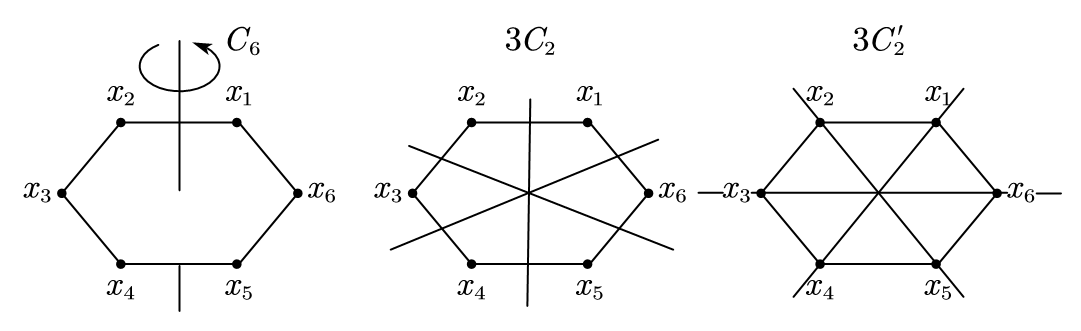
\includegraphics[width=14cm]{image/6-3-11.png}
\caption{6原子环对称性}
\end{figure}

第二种是以六边形对边连线中点构成的二重轴.\,绕它们转$180^\circ$后体系才会复原,\,典型的代表性元素:
\[C_2:\quad x_1\leftrightarrow -x_2,\,x_3\leftrightarrow -x_6,\,x_4\leftrightarrow -x_5\]

第三种是六边形的对角线作为二重轴.\,典型的代表元素:
\[C_2':\quad x_1\leftrightarrow -x_5,\,x_2\leftrightarrow -x_4,\,x_3\leftrightarrow -x_3,\,x_6\leftrightarrow -x_6\]

对称性永远都是指在某一种变换下,\,体系的某一些量具有不变的特性.\,那么我们发现,\,体系的能量函数就具有这样的特性.\,以上无论哪一个变换,\,在交换了各个$x$的角标以后,\,能量函数的表达式却恰好回到原来的表达式.\,但是对于一些不属于这个体系的对称性操作,\,比如单个$x_1\leftrightarrow x_2$.\,能量的表达式就变了.\,所以我们说体系的能量函数具有对称性.

但是体系的形状是不会具有对称性的.\,之前的示意图完全是静止状态下的苯分子\footnote{基态体系的对称性会完全等于能量函数的对称性,\,这一点也是可以被证明的.}.\,但是我们现在就是要考虑它的振动.\,作为能量函数的结果,\,其振动解是否一定具有对称的形式?\,答案显然是否定的,\,因为体系的运动由动力学方程和初始条件来决定.\,即使动力学方程是对称的,\,只要其初始条件具有不对称性,\,其解就至少有一些时刻不再对称.\,这就是说,\,\emph{对称性的原因不一定产生对称的结果}.\,这种现象就是一种广义上的\emph{对称性破缺}(symmetry breaking)现象.

但是,\,我们指出:\,如果把对称性操作理解为\emph{算符}(operator),\,它作用在一组现成的解上可以得到一种不同的运动.\,例如典型的$C_6$对称性操作,\,它把每一个原子的运动状态转移到了它的下一个原子上.\,那么我们就可以找到体系\emph{演化规律和某个对称性算符的共同本征模式}.\,这就是说,\,存在一些振动模式,\,它即是某个本征频率$\omega$下的模式,\,又恰好在某个对称性操作下(例如$C_6$)产生的运动和原来仅仅相差一个常数,\,这个常数称作\emph{本征值}(eigenvalue):
\[C_[x_i]\}=\lambda[x_i]\]

原因是简单的:\,首先如果找到了体系的一个$\omega$下的本征模式,\,那么直接用这个对称性作用在这个模式下任意次,\,显然得到的新的运动全都是原来的动力学方程的解,\,就连频率也不会改变,\,它们就全都是对应到同一个本征频率下的本征模式,\,称作\emph{简并}(degenerate)在一个频率上的模式.\,那么可以考虑得到的所有模式的组合,\,由于对称性操作连续作用有限次以后必然回到初始状态.\,故模式数必然有限.\,这样就一定可以找到合适的状态.

\newpage
例如,\,对于$C_6$,\,初始状态如果是$[x_i]_1$,\,那么至多连续作用$C_6$五次,\,第六次就回到初始状态了:
\[[x_i]_2=C_6[x_i]_1,\,[x_i]_3=C_6^2[x_i]_1,\,[x_i]_4=C_6^3[x_i]_1,\,[x_i]_5=C_6^4[x_i]_1,\,[x_i]_6=C_6^5[x_i]_1\]
\[[x_i]_1=C_6^6[x_i]_1\]

这样我们就可以构造出以下的\emph{共同本征函数}:
\[
\begin{array}{rcl}
[x_i]_{(0)}=[x_i]_1+[x_i]_2+\cdots+[x_i]_6 & \Rightarrow & C_6[x_i]_{(0)}=1\cdot[x_i]_{(0)}\\

[x_i]_{(1)}=[x_i]_1\cdot (w^1)^1+[x_i]_2\cdot (w^1)^2+\cdots+[x_i]_6\cdot (w^1)^6 & \Rightarrow & C_6[x_i]_{(1)}=w^{-1}\cdot[x_i]_{(1)}\\

[x_i]_{(2)}=[x_i]_1\cdot (w^2)^1+[x_i]_2\cdot (w^2)^2+\cdots+[x_i]_6\cdot (w^2)^6 & \Rightarrow & C_6[x_i]_{(2)}=w^{-2}\cdot[x_i]_{(2)}\\

&\cdots& \\ 

[x_i]_{(5)}=[x_i]_1\cdot (w^5)^1+[x_i]_2\cdot (w^5)^2+\cdots+[x_i]_6\cdot (w^5)^6 & \Rightarrow & C_6[x_i]_{(5)}=w^{-5}\cdot[x_i]_{(5)}
\end{array}
\]

而$w^6=1,\,w=\ue^{\ui\pi/3}$是六次单位根.\,把某个本征频率下的所有本征模式拿出来,\,对应的$C_6$算符的本征值也只有可能在以上六种值:\,六次单位根的若干幂次中选取.

同理,\,如果考虑$C_2$或者$C_2'$对称性,\,它们的本征值则更少,\,作为二次单位根仅仅只有$1$或$-1$两种可能性.\,

接下来我们可以先分析\emph{单态}(singlet).\,假设某一个角频率下仅仅只有一重简并,\,即只有一个本征模式.\,那么这个模式自己就必须同时成为$C_6,\,C_2,\,C_2'$三者的本征态.\,对于后两者有四种可能性:
\[C_2[x_i]=\pm [x_i]\quad ,\quad C_2'[x_i]=\pm [x_i]\]
\[\Rightarrow\quad \begin{bmatrix}-x_2\\-x_1\\-x_6\\-x_5\\-x_4\\-x_3\end{bmatrix} =\pm \begin{bmatrix}x_1\\x_2\\x_3\\x_4\\x_5\\x_6\end{bmatrix}\quad,\quad \begin{bmatrix}-x_5\\-x_4\\-x_3\\-x_2\\-x_1\\-x_6\end{bmatrix} =\pm \begin{bmatrix}x_1\\x_2\\x_3\\x_4\\x_5\\x_6\end{bmatrix}\]



如果两个本征值分别是$+1$和$-1$.\,那么对应的模式为:
\[[x_1,\,x_2,\,x_3,\,x_4,\,x_5,\,x_6]=x_1[+,-,+,-,+,-]\]

这样的模式恰好也是$C_6$本征值为$+1$的模式.\,对应的运动为三个相间的原子编组,\,另外三个也编组,\,两组原子反向运动的振动模式.\,用$C_2$和$C_2'$的本征值正负来标示这种模式,\,代入原来的动力学方程,\,得到:
\[-m\omega_{+-}^2A=-2kA-kA-kA\quad\Rightarrow\quad \omega_{+-}=\sqrt{\frac{4k}{m}}\]

再来考虑两个本征值都是$-1$的情况,\,这样恰好有:
\[[x_1,\,x_2,\,x_3,\,x_4,\,x_5,\,x_6]=x_1[+,+,+,+,+,+]\]

也就是所有原子都沿相同方向作相同运动.\,对应$C_6$本征值为$+1$.\,显然这样的运动就是整体作匀速旋转的运动:
\[\omega_{--}=0\]

但是另外两种情况略有不同.\,首先是两个本征值都是$+1$的情况.\,此时得到:
\[[x_1,\,x_2,\,x_3,\,x_4,\,x_5,\,x_6]=x_1[+,-,0,+,-,0]\]

抑或是两个本征值分别为$-1$和$+1$的状态.\,得到:
\[[x_1,\,x_2,\,x_3,\,x_4,\,x_5,\,x_6]=x_1[+,+,0,-,-,0]\]

我们发现,\,这些运动直接并不是$C_6$的本征态.\,但是这些运动有它存在的合理性.\,事实上画图就会发现这些运动都是可以符合动力学规律的:

\begin{figure}[H]
\centering
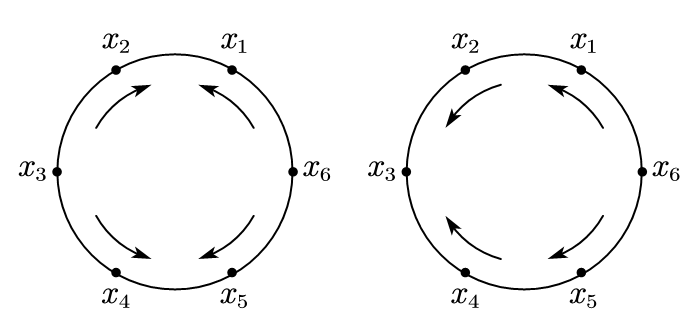
\includegraphics[width=12cm]{image/6-3-12.png}
\caption{二重简并的振动模式}
\end{figure}

每种模式的$x_1$的振动就能代表$x_1,\,x_2,\,x_4,\,x_5$四个质点的振动.\,而$x_3,\,x_6$在这两种模式下都是静止的.\,对于第一种模式,\,对$x_1$列牛顿定律:
\[-m\omega_{++}^2A=-2kA-kA\quad\Rightarrow \quad \omega_{++}=\sqrt{\frac{3k}{m}}\]
\[-m\omega_{-+}^2A=-2kA+kA\quad\Rightarrow \quad \omega_{-+}=\sqrt{\frac{k}{m}}\]

正因为这些运动合理,\,但又不是$C_6$的本征态,\,所以其实它们根本就不像最初假设的那样,\,是两个本征频率$\omega_{++},\,\omega_{-+}$下的单态,\,而是各存在二重简并.\,显然我们把$C_6$作用在这两个态上各一次就是与它简并在同一个频率上的另一个独立振动模式,\,如果设$x_1=A\ue^{\ui\omega t}$:
\[[x_i]_{++}=[+,-,0,+,-,0]A\ue^{\ui\omega_{++} t}\quad\Rightarrow\quad C_6[x_i]_{++}=[0,+,-,0,+,-]A\ue^{\ui\omega_{++} t}\]
\[[x_i]_{-+}=[+,+,0,-,-,0]A\ue^{\ui\omega_{-+} t}\quad\Rightarrow\quad C_6[x_i]_{-+}=[0,+,+,0,-,-]A\ue^{\ui\omega_{-+} t}\]

恰好,\,作用两次是徒劳的.\,两次旋转以后的运动可以用前两次的运动组合形成:
\[C_6^2[x_i]_{++}=-[x_i]_{++}-C_6[x_i]_{++}\quad:\quad [-,0,+,-,0,+]=-[+,-,0,+,-,0]-[0,+,-,0,+,-]\]
\[C_6^2[x_i]_{-+}=-[x_i]_{-+}-C_6[x_i]_{-+}\quad:\quad [-,0,+,+,0,-]=-[+,+,0,-,-,0]-[0,+,+,0,-,-]\]

从而我们就完整地找到了体系的六个本征模式:
\[\omega_{--}=0\quad:\quad [x_i]_{--}=[+,+,+,+,+,+]vt\]
\[\omega_{-+}=\sqrt{\frac{k}{m}}\quad:\quad [x_i]_{-+}=[+,+,0,-,-,0]A\ue^{\ui\omega_{-+} t}\quad,\quad C_6[x_i]_{-+}=[0,+,+,0,-,-]A\ue^{\ui\omega_{-+} t}\]
\[\omega_{++}=\sqrt{\frac{3k}{m}}\quad:\quad [x_i]_{++}=[+,-,0,+,-,0]A\ue^{\ui\omega_{++} t}\quad,\quad C_6[x_i]_{++}=[0,+,-,0,+,-]A\ue^{\ui\omega_{++} t}\]
\[\omega_{+-}=\sqrt{\frac{4k}{m}}\quad:\quad [x_i]_{+-}=[+,-,+,-,+,-]A\ue^{\ui\omega_{+-} t}\]

事实上我们只看到了问题的一个局部.\,关于复杂体系小振动背后的对称性分析是一个内容非常丰富的专题.\,它涉及到关于对称性的\emph{群论}(group theory)和对于振动在对称性操作下演化的\emph{群表示论}(group representation theory).\,它在原子分子物理,\,固体物理,\,乃至粒子物理中都有着非常广泛的应用.

对于苯分子的振动模式我们也做了过多的简化,\,下面的表是较完整地考虑碳原子和氢原子间共$12$个原子,\,在三维空间中各做三自由度运动而形成的共$36-6=30$个振动模式.\,减$6$是因为有$6$个自由度是整体的平动和转动而不是振动.\,根据对称性,\,一共有$20$种振动模式.\,其中有$10$种为二重简并.\,分子的振动光谱一般在红外线波段:
\begin{figure}[H]
\centering
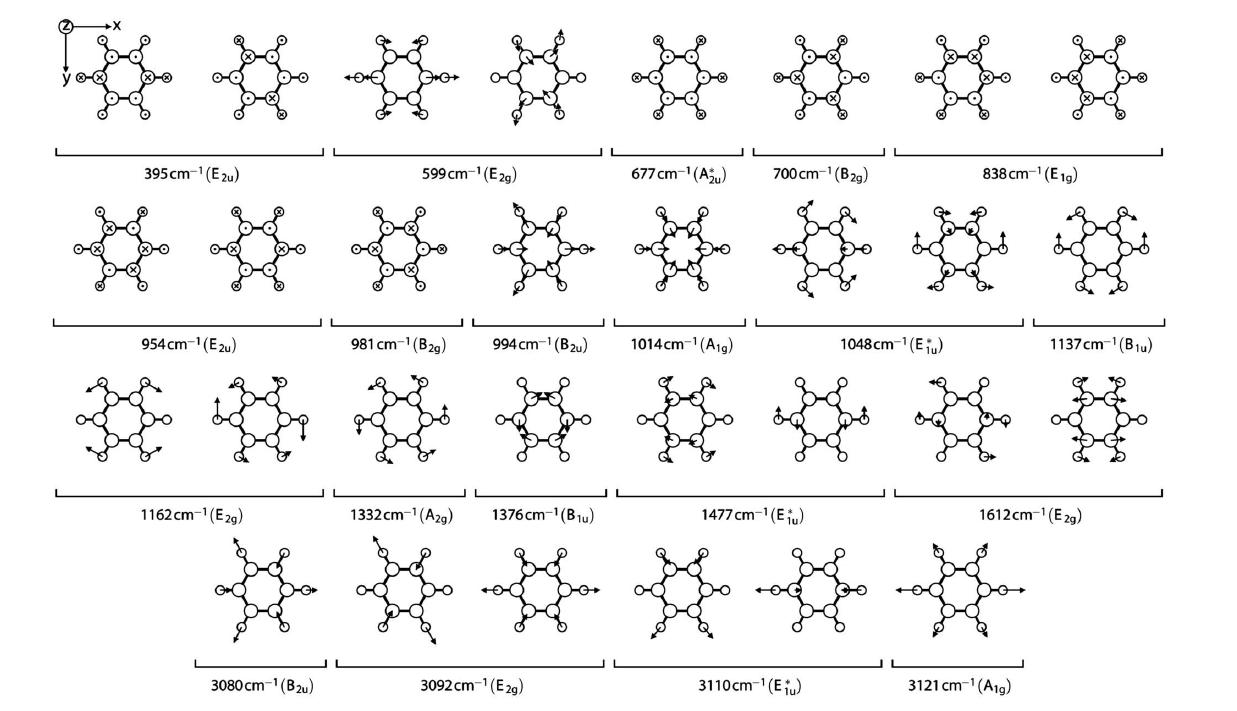
\includegraphics[width=17cm]{image/6-3-9.png}
\caption{苯分子的完整振动模式}
\end{figure}

利用原子间作用力的经验函数就可以得到各个本征角频率$\omega$.\,而由量子力学中的原理,\,振动的能量实际上是量子化的:
\[E_n=\left(n+\frac{1}{2}\right)\hbar\omega\]
苯分子的吸收光谱和发射光谱中对于相邻两个能级能量差的光子就会有共振吸收的现象:
\[\Delta E=h\nu =\hbar \omega\]

可见其实就是当电磁波的频率恰好与振动频率吻合时发生共振吸收:
\[\nu=\frac{\omega}{2\pi}\]
\newpage


\section{非线性摄动*}



\section{格波}

让我们考虑两个十分经典的\emph{固体物体}(solid state physics)问题:\,声音的本质是什么?\,固体热运动的本质是什么?\,我们可能会得到一个惊人的答案:\,两者的本质,\,都是晶格的振动.

固体,\,一般是晶体,\,它的描述方法,\,也需要照顾到电子的行为,\,也需要照顾余下的原子实---它占据着主要的质量与动能---的运动形式.\,如果把目光仅仅放在原子实上,\,认为原子实是在格点的平衡位置附近做小振动.\,而这个运动的动力学成因,\,必然是来自于初始条件和原子之间可以类比为弹簧的线性作用力.\,这样去思考问题的话,\,也许具体的计算还是困难的,\,但至少我们会有以下三个结论:

一:\,这个运动一定是牵一发而动全身的.\,一个原子的振动会带动其它原子的振动,\,一个地方的振动会带动另一个地方的振动,\,这其实就是固体可以传热和传声的原理.\,而且不出意外的,\,一般传热性能越好的固体,\,声速也就越快.\,天然材料中金刚石就是在两个方面都具有卓越性能的典型:\,它的声速高达$12000{\rm m/s}$,\,在元素单质方面仅仅次于在自然界不以单质形式存在的金属铍($13000{\rm m/s}$),\,是铁的两倍多.\,而热导率则是达到了惊人的$2000{\rm W/m\cdot K}$,\,为金属中导热性能优异的银的约五倍.

二:\,有规则的这种运动形成了声波.\,也就是宏观问题中看似连续的声波,\,在微观看来其实就是一个个分立的原子在因为弹性力而做多自由度的小振动,\,而不再具有连续性.\,这种运动就叫做\emph{格波}(lattice wave).

三:\,无限不规则的声波进行叠加就形成了热运动.\,基于这一点,\,我们其实不应该把热运动分解为每一个原子各做一个独立简谐振动,\,这样的统计方法是不能给出正确的关于固体的热学结果的,\,因为这些简谐振动根本就不``独立''.\,从爱因斯坦时代开始,\,把热运动分解为真正声波的叠加,\,并且对声波的能量进行量子化,\,称作\emph{声子}(phonon),\,这才真正能开始解释关于固体的热容等等初步的实验结果.

这一节我们暂时无法得出这些深刻结果的计算过程.\,但至少,\,我们可以尝试在完全经典的情况下对两个简化问题给出完整的动力学求解方法.

第一个问题就是\emph{一维原子链}(1D atomic chain)问题.\,把质量为$m$的物块和劲度系数为$k$的弹簧无限串接形成下图所示的体系.

\begin{figure}[H]
\centering
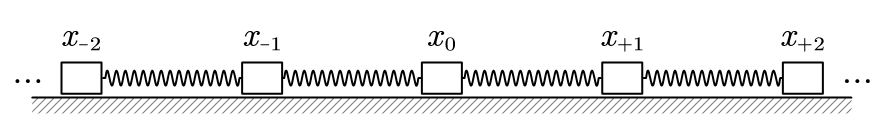
\includegraphics[width=15cm]{image/6-3-13.png}
\caption{一维原子链}
\end{figure}

这样的体系的动力学方程写作:
\[m\ddot{x}_i=-2kx_i+kx_{i+1}+kx_{i-1}\]

这样一个方程的求解其实非常类似于之前的对称性分析法.\,这里体系的对称性为平移一个单元.\,那我们就设想体系的状态为平移算符的本征态,\,即每一个物块的振动都恰好是其前一个(左边的那个,\,指标比它小一的那个)的$\lambda$倍.\,只不过这里的$\lambda$其实是一个相位因子$\ue^{\ui \varphi}$罢了.\,那么我们猜一个本征频率为$\omega$,\,在平移算符下本征值为$\lambda$的解,\,显然$\omega$就会是$\lambda$的函数:
\[x_i=\lambda^i A\ue^{\ui\omega t}\]

代入原方程,\,命$\omega_0=\sqrt{k/m}$就可以得到:
\[\frac{\lambda+\lambda^{-1}}{2}=1-\frac{\omega^2}{2\omega_0^2}\]

若$\lambda$为实数,\,不管是$|\lambda|>1$还是$|\lambda|<1$都不是我们希望得到的结果,\,这样在$i\to+\infty$和$i\to-\infty$两个方向一个振幅指数衰减,\,一个指数爆炸.\,那么根据因果律和能量守恒可以判断,\,指数爆炸那一侧是受到外力开始起振的那一侧,\,这个波根本就不能在原子链上传播,\,而是传着传着振幅就衰减掉了.\,此时等号左侧是一个绝对值大于$1$的实数.\,故我们发现当$\omega\geq 2\omega_0$时对应的波无法在一维原子链上传播.\,这个频率$\omega_c=2\omega_0$就叫做\emph{截止频率}(cut-off frequency).\,恰好为截止频率时,\,$\lambda=-1$,\,也就是这样的波虽然可以形成,\,但任何相邻两个原子振动方向彻底反向,\,它其实是一种``驻波'',\,原则上也没有在传播.

那么就只剩下$\omega\leq \omega_c$的波可以在一维原子链上传播.\,把$\lambda$写成$\ue^{\ui \varphi}$.\,我们得到:
\[\cos\varphi=1-\frac{\omega^2}{2\omega_0^2}\quad \Rightarrow \quad \omega=2\omega_0\left|\sin{\frac{\varphi}{2}}\right|\]

相邻两个原子的相位差应当是一个$\varphi\in (-\pi,\pi)$内的数.\,这是因为如果$A$比$B$相位大一个$\pi+\delta$,\,那么也可以解释为$A$比$B$相位小一个$\pi-\delta$.\,所以如果是截止频率的临界情况,\,我们也只能说相邻的原子反相,\,至于谁比谁大也是无从判断的,\,这是格波的特性.

对于上式我们更喜欢写为\emph{色散关系}(dispersion relation)的形式.\,就是说把自变量改为\emph{波矢}(wave vector).\,设相邻原子距离为$l$,\,那么产生的相位差$\varphi$可以由波矢来产生:
\[Kl=\varphi\quad,\quad K\in\left(-\frac{\pi}{l},\,\frac{\pi}{l}\right)\]

\begin{wrapfigure}[13]{o}[-10pt]{6cm}
\centering
\vspace{-1.5cm}
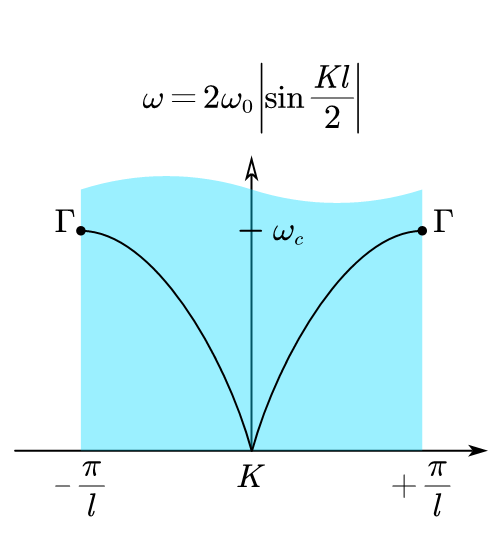
\includegraphics[width=6cm]{image/6-3-14.png}
\caption{色散关系}\label{6-3-14}
\end{wrapfigure}
上面这个$K$应当处于的空间称作\emph{布里渊区}(Brillouin zone).\,它告诉我们,\,在一维原子链上传播的格波在频率和波矢上都是受限的.\,其函数图像和表达式如图\ref{6-3-14}.

色散曲线上每一个点都代表一种能够在一维原子链上传播的振动模式:
\[x_i=A\ue^{\ui(\omega t+iKl)}\]

此时两个极限是值得关注的:

一是,\,在短波极限:\,波长最短就是当$Kl=\pi$时,\,此时波长$\Lambda=2\pi/K=2l$时,\,向左和向右延伸的色散曲线到达最高点$\Gamma$.\,但尤其要注意两个$\Gamma$点实质上就是同一个点,\,对应完全相同的状态.\,可以想想把第一布里渊区卷做一个圆柱,\,让两个$\Gamma$点重合.\,对应的相邻原子彼此反相的``驻波''形式.\,也就是说如果让$K>0$的右行波的$K$持续增加以跨越$\Gamma$点,\,波就演化为左行波了.\,个中缘由在于$K$的正负指称的速度其实是\emph{相速度}(phase velocity),\,但在判断波的传播方向时,\,其实\emph{群速度}(group velocity)才是更加合理的选择.\,它被定义为:
\[v_g=\frac{\ud \omega}{\ud K}\]

其中的原理我们将在流体的相关波动章节中简介.

二是,\,在长波极限:\,$\Lambda\gg l$.\,此时$Kl$时一个小量,\,可以对$\sin$使用近似,\,物理上代表相邻两个原子几乎是以相同的方式运动,\,微观波变成了宏观的波:
\[\omega=\omega_0Kl\]

这就给出了波的传播速度:
\[v=\frac{\omega}{K}=\omega_0 l=\sqrt{\frac{k}{m}}l\]

这个结果与宏观波速公式$v=\sqrt{E/\rho}$是完全一致的.\,且看之后弹性体章节的分析.

\vspace{1cm}

最后我们还看看\emph{双原子链}(diatomic chain)与以上\emph{单原子链}(monoatomic chain)产生的并不平凡的区别.\,双原子链就意味着虽然其平移周期还是$l$,\,但每一个单元内部出现了两个待求解的坐标.\,我们让两个原子质量分别为$M,\,m$,\,弹簧劲度系数依然为$k$:
\begin{figure}[H]
\centering
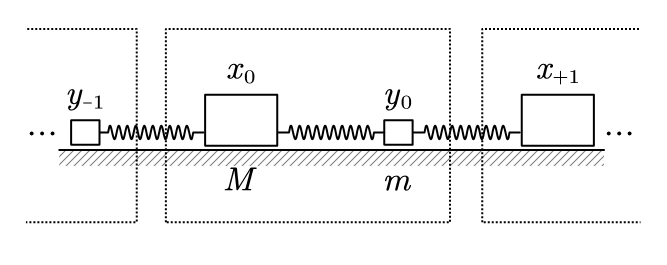
\includegraphics[width=10cm]{image/6-3-15.png}
\caption{双原子链}
\end{figure}

那么对应的动力学方程写作:
\[M\ddot{x}_i=-2kx_i+ky_i+ky_{i-1}\]
\[m\ddot{y}_i=-2ky_i+kx_i+kx_{i+1}\]

由于有单原子链的经验.\,我们让$\omega_0=\sqrt{k/2M}$\footnote{即先忽视$m$的存在让弹簧直接串联.},\,而$m=\beta M$.\,并直接设解为:
\[x_i=A\ue^{\ui(\omega t+iKl)}\quad,\quad y_i=B\ue^{\ui(\omega t+iKl)}\]\

其中$A$和$B$是复振幅可以差一个相位.\,那么这就给出:
\[
\begin{array}{rcrc}
(4\omega_0^2-\omega^2)A&+&-2\omega_0^2(1+\ue^{-\ui Kl})B&=0\\
-2\omega_0^2(1+\ue^{\ui Kl})A&+&(4\omega_0^2-\beta\omega^2)B&=0
\end{array}
\]

这个方程组$A,\,B$的解不为零的条件就是:
\[(4\omega_0^2-\omega^2)(4\omega_0^2-\beta\omega^2)=4\omega_0^4(1+\ue^{\ui Kl})(1+\ue^{-\ui Kl})=16\omega_0^4\cos^2\frac{Kl}{2}\]

在$\beta$是个小量的情况下,\,我们可以近似地求解这个方程.\,在任意$K$下这个方程与单原子链不同,\,它$\omega^2$总是有两个解.\,第一个解发生在$\omega$与$\omega_0$量级相当的情况下,\,此时$4\omega_0^2-\beta\omega^2\approx 4\omega_0^2$.\,近似可以得到:
\[\omega=2\omega_0\left|\sin{\frac{Kl}{2}}\right|\]

可以发现这个解与只含$M$的单原子链的结果并没有什么区别.\,所以其实是这种模式下,\,主要的动力学效果由$M$承担,\,$m$则几乎平衡在两侧的$M$中间.\,两个相邻的$M$之间的两段弹簧几乎就是直接串联在一起,\,同时伸长同时缩短,\,感受不到很轻的$m$的影响.

而另外一个解则发生在$\omega\gg \omega_0$的极端情况下,\,此时$4\omega_0^2-\omega^2$本是一个绝对值很大的负数,\,它$\approx -\omega^2$.\,但是与另一个因子$4\omega_0^2-\beta\omega^2$相乘时又回到正的$\omega_0^4$量级的等式右侧了.\,从而乘的因子其实很接近零:
\[4\omega_0^2-\beta\omega^2\approx 0\quad\Rightarrow \quad \omega\approx \frac{2\omega_0}{\sqrt{\beta}}\]

为了更精确地找到这个频率与$K$的函数关系,\,我们把原方程的$4\omega_0^2-\omega^2$项除到等号右边,\,并近似:
\[\omega\approx \frac{2\omega_0}{\sqrt{\beta}}\cdot\sqrt{1+\beta\cos^2\frac{Kl}{2}}\]

\begin{wrapfigure}[13]{o}[-10pt]{8cm}
\centering
\vspace{-0.5cm}
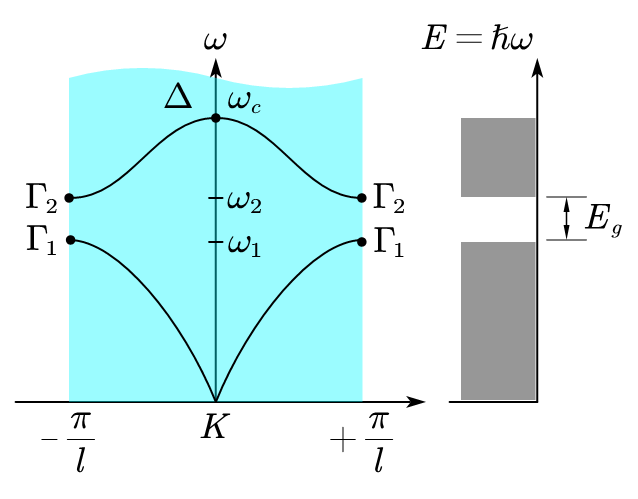
\includegraphics[width=8cm]{image/6-3-16.png}
\caption{声学支与光学支}\label{6-3-16}
\end{wrapfigure}
这样的两组解看似近似,\,但是其实在特征点处的性质和坐标又是完全准确的.\,特征点就是指波矢为零$K=0$和波矢为$\pm \pi/l$的布里渊区中心和边界上的点.\,我们把两组$\omega(K)$关系画成色散曲线如图\ref{6-3-16}.\,对应的特殊点$\Gamma_1,\,\Gamma_2,\,\Delta$对应的特殊频率为:
\[\omega_1=2\sqrt{\frac{k}{2M}}\quad ,\quad \omega_2=2\sqrt{\frac{k}{2m}}\]
\[\omega_c=2\sqrt{\frac{k}{2\mu}}\;(\mu=\frac{Mm}{M+m})\]

现在终于可以发现,\,多出来的第二组解,\,对应了在原来的色散曲线上方又多出来一支.\,这一支在$\Delta$的行为具有代表性:\,即使$K=0$,\,即相邻两个单元之间完全没有相位差.\,但是依然有很大的角频率.\,也就是这个振动并没有传播,\,而从角频率的表达式来看,\,其实就是每一个单元内部两个物体在弹性力作用下做二体小振动.\,而从$\Gamma_2$到$\Delta$点这样一段色散曲线对应的各个波动模式下,\,十分显著的一点就是轻的原子一定要主动振动起来而且与相邻的重原子根接近反相而不是同相.\,最边缘的$\Gamma_2$点则只有轻的原子在振动.\,这样的模式的频率,\,其实与上一节讨论过的分子振动频率相当,\,就在光的红外线频段,\,故把这样的一支振动模式称作色散曲线的\emph{光学支}(optical branch).

所以原来单原子链的保留支,\,特点是从$\omega=0,\,K=0$延续到布里渊区边缘的$\Gamma_1$,\,就相应的被称作\emph{声学支}(acoustic branch).\,因为在长波极限$K\to 0$下,\,这个模式的轻重原子之间是没有相位差的,\,而不是像光学支那样反相,\,这样就相当于宏观地看整个原子链在较大范围内做宏观平移.\,形成的波就是常规意义下的声波.\,在声学支模式下,\,轻的原子跟随重的原子而运动,\,相邻轻重原子更加接近同相而不是反相.\,而极限点$\Gamma_1$对应的情况是只有重原子在振动,\,轻原子全部静止了.

最后我们指出,\,简单的计算产生的结果中还蕴含着意义非凡的一个物理图像.\,那就是\emph{能带}(energy band)结构的产生.\,在这里我们着眼的是晶格上的波动,\,色散曲线上每一个点都代表一种可能的波动模式,\,其振幅,\,在经典物理中,\,由初始条件决定,\,且是可以连续变化的.\,但是量子理论预言,\,这个能量实则在低能量时量子化:
\[E_n=\left(n+\frac{1}{2}\right)\hbar\omega\]

从而色散曲线的这一副图,\,实际上也代表量子化的振动的\emph{元激发}(elementary excitation)的能量单位与$K$的关系图.\,更有甚者,\,如果我们不是去考虑晶格振动的动能加势能的元激发,\,而是去考虑在晶格间运动的电子,\,它的能量也会产生非常类似的但更复杂的能带结构\footnote{会往上产生更多能带.},\,毕竟电子在其中的描述也应当使用物质波,\,它具有波矢$K$和相应的能量$E(K)$.\,而为什么这个$E(K)$的函数也会产生类似的行为,\,这一点可以纯粹从电子满足的\emph{薛定谔方程}(Schr\"odinger equation)和对称性分析出发得到.\,在介质中的电子的波矢$K$其实也是受限的.\,而同一个$K$对应的能量也可以有多个,\,分别在不同分支的色散曲线上.\,故我们把每一条色散曲线对应的可取能量区间叫做\emph{允带}(allowed band).\,而允带之间没有对应状态的能量区间叫做\emph{禁带}(forbidden band).\,两个相邻的允带之间的禁带宽度就是\emph{带隙}(band gap).

这样一种全新的看待振动的能量,\,电子的能量的理论就是能带论.\,尤其是把电子视作物质波,\,利用量子力学完整地计算固体中的电子的运动,\,从而非常好地解释了历史上残留的金属电导率,\,热导率相关的疑问并很好地带动半导体物理学的成熟的理论,\,以它的主要缔造者:\,瑞士-美国物理学家布洛赫\,命名为\emph{布洛赫理论}(Bloch theory).

能带结构是一种介于\emph{自由电子}(free electron)和\emph{紧束缚电子}(tight-binding electron)之间的存在形式.\,在真空中的自由电子满足:
\[E=\frac{\hbar^2K^2}{2m}\]

其能量完全可以连续的改变.\,但是在束缚态上,\,如氢原子外的电子,\,简单地由玻尔模型,\,电子的能量被量子化为能级结构:
\[E=-\frac{me^4}{8n^2\varepsilon_0^2h^2}=-\frac{13.6{\rm eV}}{n^2}\]

那么在金属中的电子,\,微观上自由:\,可以脱离金属原子的束缚而传导,\,但宏观上,\,本质又是被束缚的:\,被所有原子核共同产生的吸引力束缚在金属内部.\,所以就体现出一种折衷:\,紧束缚的能级展开为能带,\,具有一定的能量连续变化的范围.\,但是能带与能带之间依然是分立的,\,没有像真空那样连成一片.


% %!TEX root = ../physical-olympics-2.tex
\chapter{万有引力}


\section{有心力下运动}

天体运动中起到核心作用的相互作用力都是\emph{有心力}(central force),\,事实上不光是天体运动,\,任意两个可以近似为质点的物体之间的相互作用力,\,根据牛顿第三定律的要求,\,其受力方向都必须沿着两个物体的连线方向.\,那么我们只要做两个要求,\,这就构成了一个有心力问题:

一是,\,这个力必须是保守力,\,即,\,它必须由势能生成:
\[V(\bs{r}_1,\,\bs{r}_2):\quad\,\bs{F}_1=-\nabla_1V\;,\,; \bs{F}_2=-\nabla_2V\]

根据我们之前的说法,\,根据对称性或牛顿第三定律,\,这个势能其实就是两个质点连线距离$R$的函数$V(R)$.\,而以$1$为中心向$2$引$\bs{R}$矢量,\,则:
\[\bs{F}_2=-V'(R)\bs{e}_{\bs{R}}=F(R)\bs{e}_{\bs{R}}\]

二是,\,中心物体$1$必须不动或者是近似不动.\, $1$不动是指有外力作用在$1$上以维持其静止.\,但$2$上不应该有这样的外力,\,而仅仅是在$1$对$2$产生的$\bs{F}_2$作用下做运动.\,$1$近似不动是比如考虑太阳系这种典型情况,\,太阳虽然受到多个行星对它的万有引力,\,但是由于自己质量过重从而近似是不动的.\,即使是地球月亮构成的二体问题,\,地球和月亮并不一定能认为都不动,\,我们也有相应的转化为有心力问题的方法,\,见后.\,最后当然,\,也有一些更简单的情况,\,$2$受到一些更复杂的体系对它的力构成了有心力$F(R)$,\,比如弹性绳对绳端质点的拉力.



\section{万有引力下运动}

\section{二体与潮汐}


% %!TEX root = ../physical-olympics-2.tex
\chapter{刚体}


\section{刚体的物理描述}
近代以前人们意识到了物质世界的\emph{连续性}(continuum),\,同时针锋相对地也提出了\emph{原子论}(atomism).\,原子最简单的模型就是质点,\,而调和物质连续性与原子学说的中间模型就是\emph{刚体}(rigid body)模型.\,刚体是不允许形变发生的系统.\,由牛顿力学对质点的讨论推广到质点系的讨论,\,使我们也很容易将相关结论进一步推广到刚体.

由于刚体上一点受力,\,则整体同时运动起来,\,这个模型与相对论力学体系是不兼容的.\,具体来说,\,相互作用必须以有限的速度传播,\,否则就违背了因果律.\,刚体不符合因果律这一时空的固有结构.\,在很多相对论情境下将招致矛盾的结果.

刚体的物理学量是哪一些呢?\,必要的内禀的属性是其质量的分布.\,某一默认时刻$t_0$刚体占据了空间区域$\Omega_0$,\,由大量体积微元$\ud V$(记做$\ud^3\bs{R}_0$)组成,\,则刚体的总质量为:
\[m=\int\limits_{\Omega_0}\rho(\bs{R}_0)\ud^3\bs{R}_0=\int\limits_{\Omega_0}\ud m\]

\begin{wrapfigure}[17]{o}[-10pt]{7cm}
\vspace{-0.4cm}
\centering
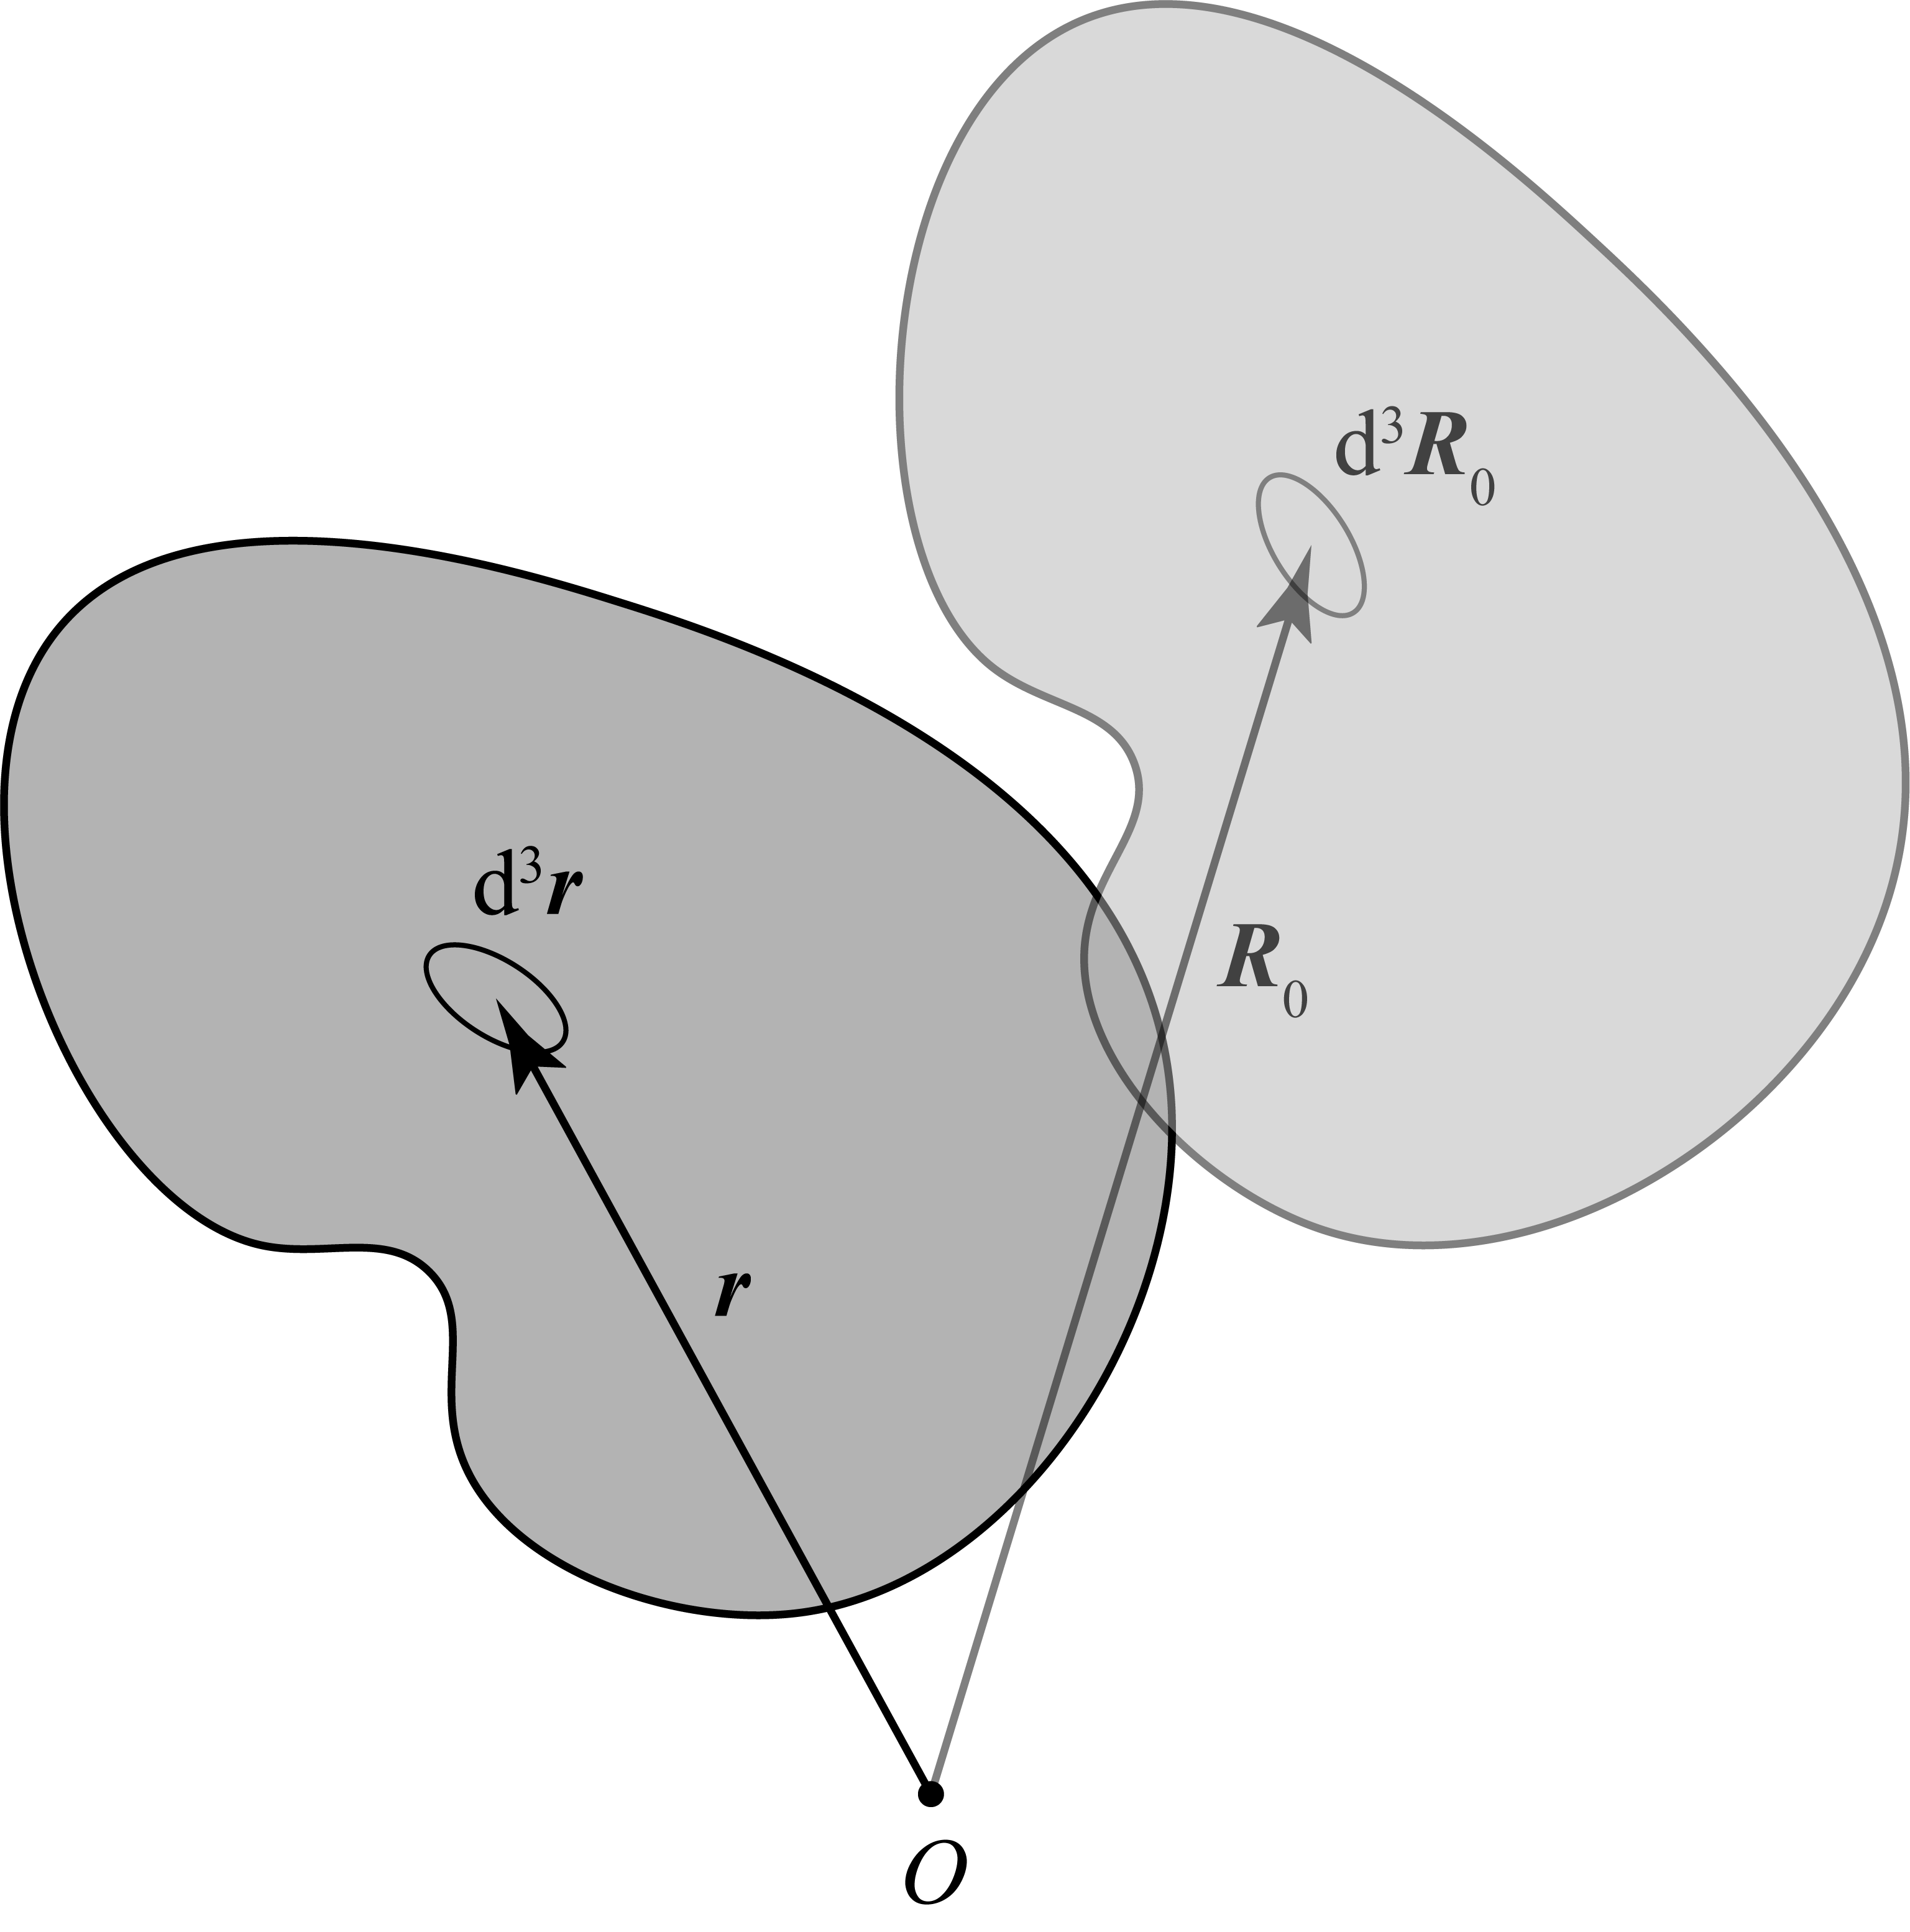
\includegraphics[width=7cm]{image/6-6-1.png}
\caption{刚体的描述}
\end{wrapfigure}
随着刚体的运动,\,原来在$\bs{R}_0$处的体积元现在在$t$时刻位于$\bs{r}$处,\,整个刚体的运动由一个多元映射来定义:
\[f:\quad \bs{R}_0,\,t\;\;\longrightarrow\;\; \bs{r}(\bs{R}_0,\,t)\]

刚体的刚性的要求,\,使得这个映射必须保持体积元的不变性:
\[f:\quad \ud^3\bs{R}_0\in\Omega_0\;\;\longrightarrow\;\; \ud^3\bs{r}\in\Omega \quad ;\quad \ud^3\bs{R}_0=\ud^3\bs{r}=\ud V\]

而且所有这个体积元内的所有内禀属性,\,这里包括密度都不能变.\,所以质量元$\ud m$也是不变的.\,从而刚体具有不变的总质量.\,马上就会发现,\,\emph{质量几何}(mass geometry)对刚体的动力学来说也十分重要.\,质量几何研究质量对特定原点$O$的各级\emph{矩}(moment).\,其中零级矩即为质量:
\[M^0=m=\int\limits_\Omega \ud m\]

一级矩是个矢量,\,它定义了刚体的\emph{质心}(center of mass)的位置:
\[M^1_i=mr_{Ci}=\int\limits_\Omega r_i\ud m\]
\[\bs{r}_C=\frac{\int\limits_\Omega \bs{r}\ud m}{\int\limits_\Omega \ud m}\]

二级矩则是一个张量,\,它的九个分量代表\emph{惯量积}(product of inertia):
\[M^2_{ij}=\int\limits_\Omega r_ir_j\ud m\]

这些矩和原点的选取有关,\,随着刚体的运动也会不断变化,\,这三阶矩的信息对刚体动力学来说就是充分的了,\,通过后面的动力学可以发现,\,刚体的运动完全依赖于外力和这三阶矩.\,如果要研究广义相对论里的引力波辐射问题,\,更高阶的矩才变得重要起来.

刚体的运动可以被我们更精确地描述,\,在$t_0$时刻建立固定在刚体上,\,沿$x,y,z$三方向的单位矢量$\bs{e}_1,\bs{e}_2,\bs{e}_3$,\,那么刚体的运动同时也把三个矢量旋转到新的三个方向:
\[f:\quad \bs{e}_i\;\longrightarrow\; \bs{\varepsilon}_i\]

这三个矢量仍然要互相垂直,\,且长度为一.\,这在数学上导致了可以通过这三个矢量的导数定义\emph{角速度}(angular velocity)矢量的结果:
\[\dot{\bs{\varepsilon}}_i=\bs{\omega}\times\bs{\varepsilon}_i\]

\begin{wrapfigure}[15]{o}[-10pt]{7cm}
\vspace{-0.7cm}
\centering
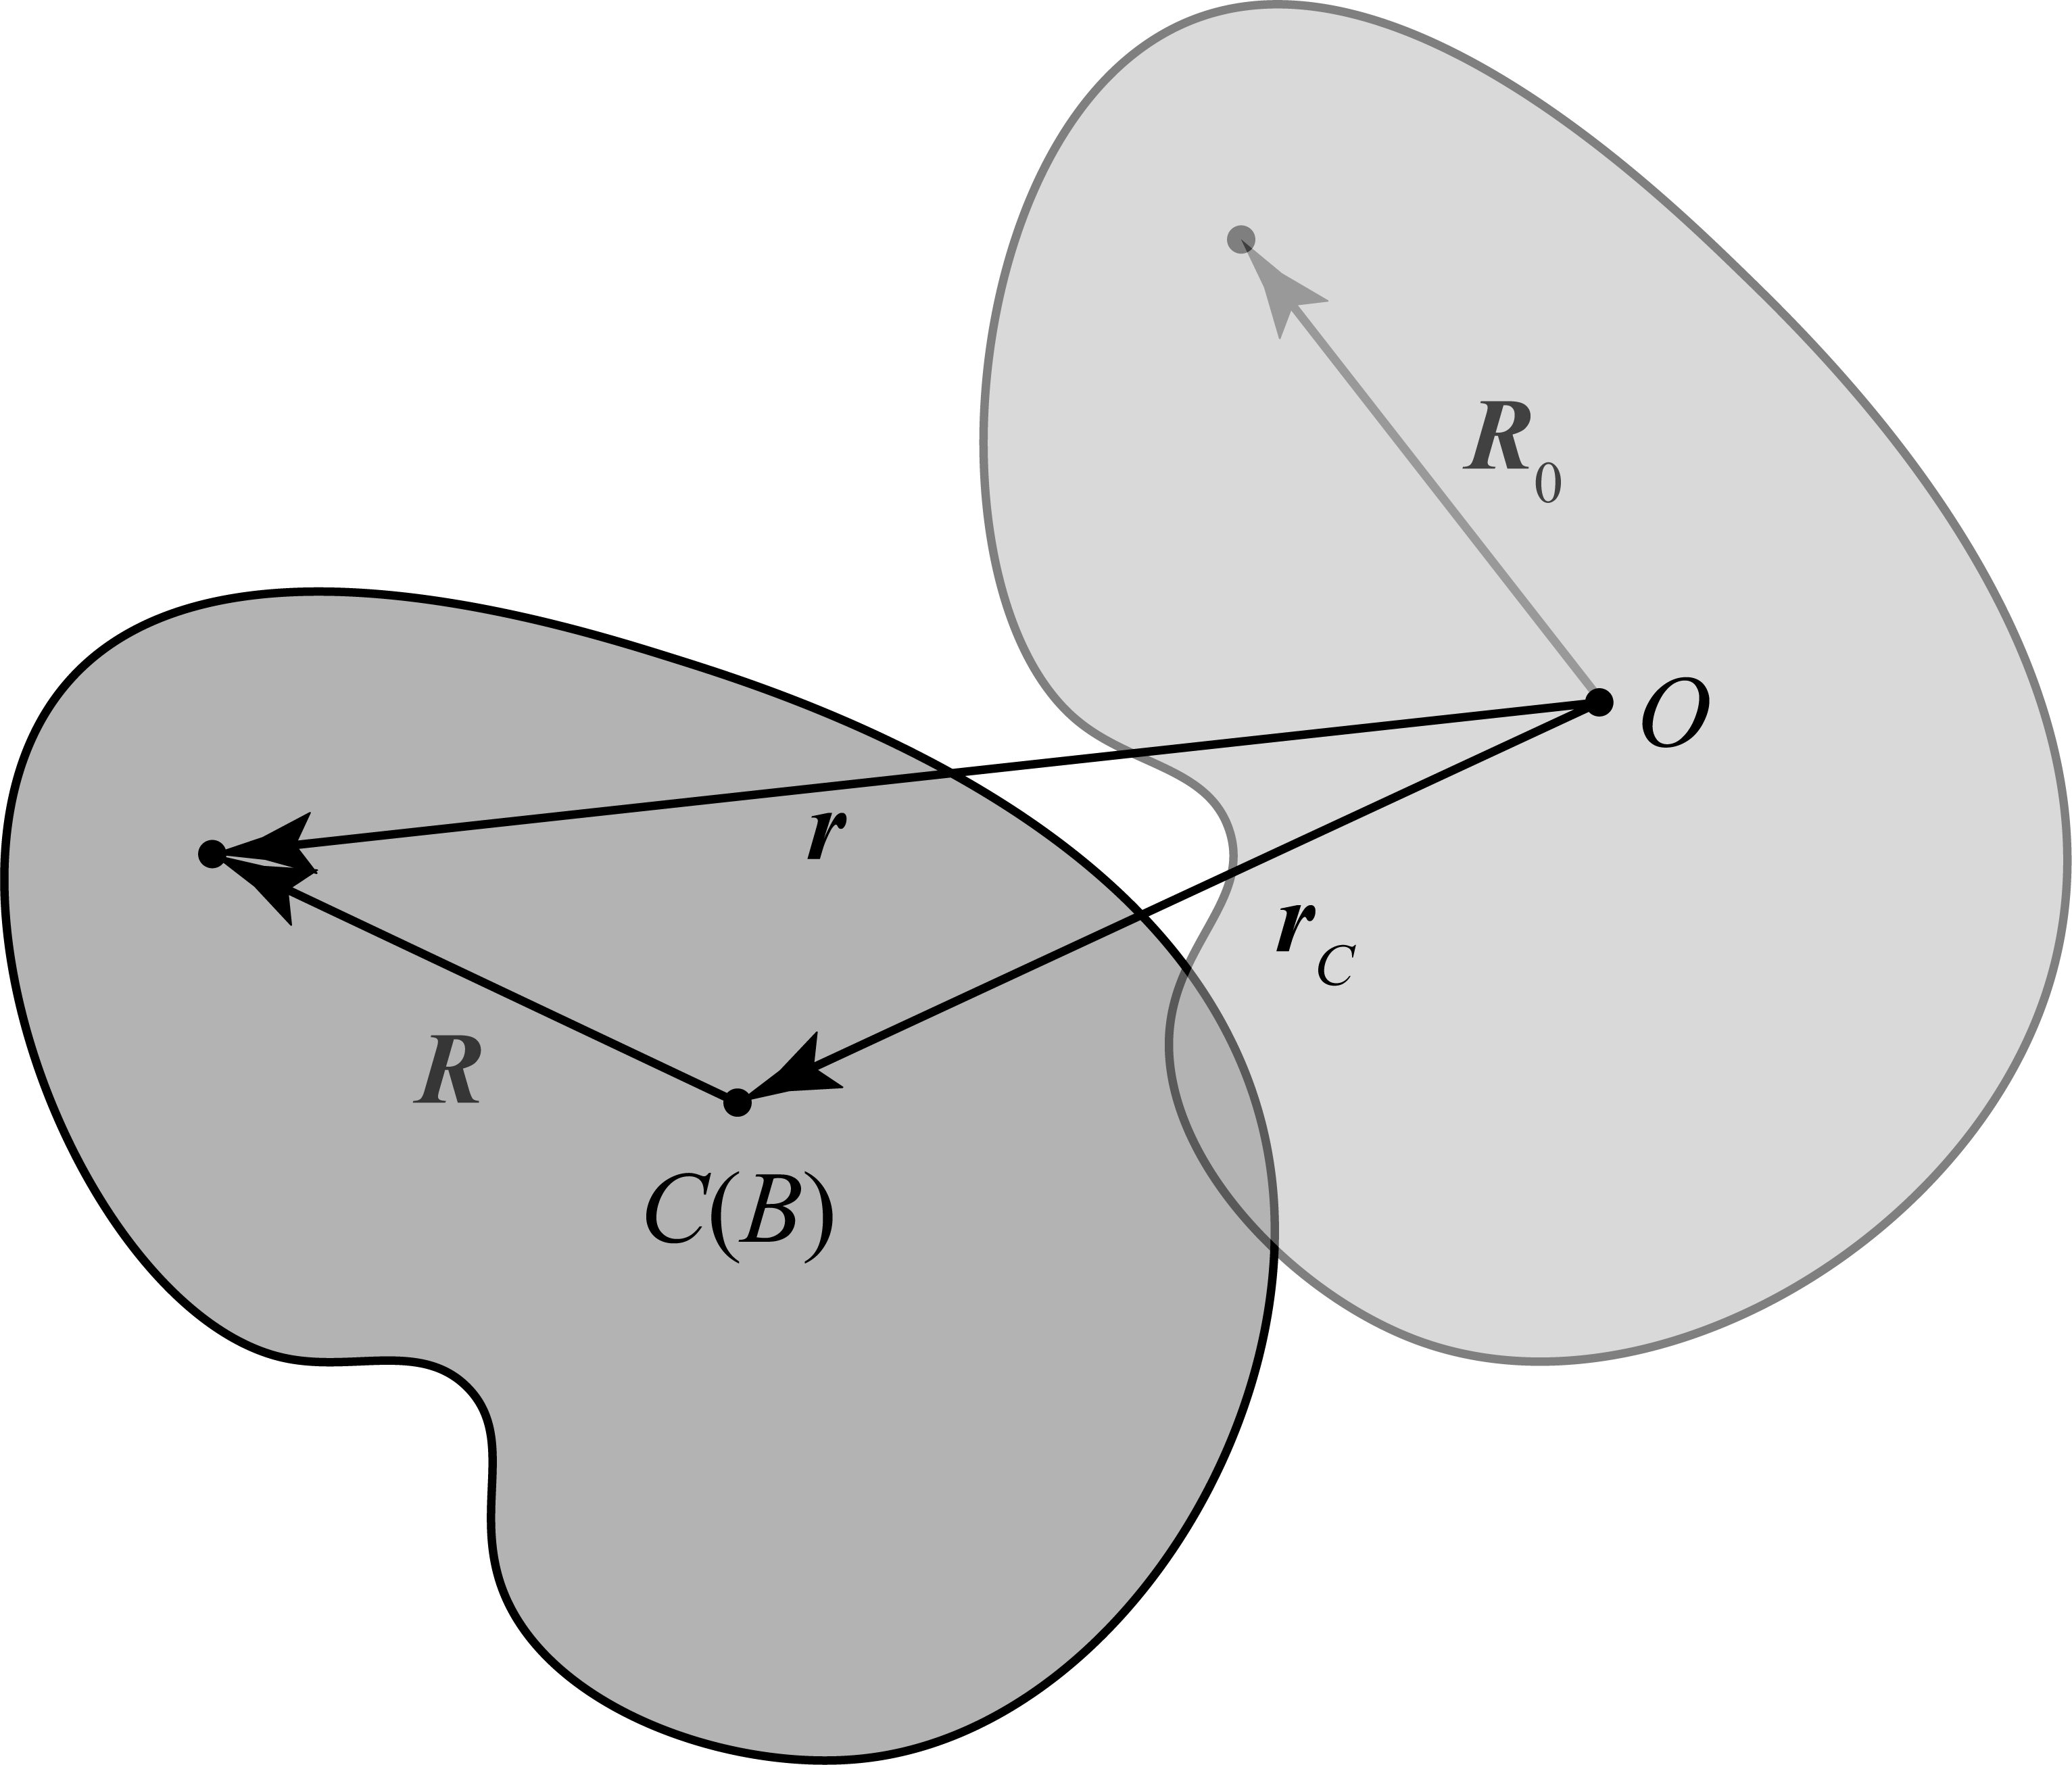
\includegraphics[width=7cm]{image/6-6-2.png}
\caption{基点法}
\end{wrapfigure}
十分类似于旋转参考系的变换的运动学,\,刚体的运动实际上就是有一个唯一的旋转参考系固连在刚体上,\,以后称作\emph{刚体系}(reference system of rigid body),\,要研究的刚体上各个点速度实际上就是刚体系中定点的运动.\,于是习惯上我们采用\emph{基点法}(method of base point)来计算刚体上任意点的运动学量.\,定义\emph{基点}(base point)为$t_0$时刻$\bs{R}_0=\bs{0}$的点$B$,\,之后的位矢为$\bs{r}_B$,\,对应的基点速度加速度为$\bs{v}_B,\,\bs{a}_B$,\,而刚提上待研究的点相对基点的位矢为$\bs{r}-\bs{r}_B=\bs{R}$,\,那么该点的速度加速度即为:
\[\bs{v}=\bs{v}_B+\bs{\omega}\times\bs{R}\]
\[\bs{a}=\bs{a}_B+\bs{\omega}\times(\bs{\omega}\times\bs{R})+\dot{\bs{\omega}}\times\bs{R}\]

出于动力学的考虑,\,基点$B$一般就取做质心$C$.\,作用在刚体上$\bs{r}$处的力$\bs{F}$固然对原点会有力矩$\bs{M}$,\,但是为了研究使刚体自身转动的效应,\,考虑到这个力同时也会使得质心运动起来,\,故我们重视这个力相对质心的力矩$\bs{M}_C$:
\[\bs{M}=\bs{r}\times\bs{F}\]
\[\bs{M}_C=\bs{R}\times\bs{F}\]

刚体受到一个力系${\bs{F}_i}$的作用,\,那么以下六个定理则来自于之前的动力学理论:
\[\sum_i\bs{F}_i=\frac{\ud \bs{p}}{\ud t}\quad ; \quad \sum_i\bs{F}_i=m\bs{a}_C\]
\[\sum_i \bs{v}_i\cdot \bs{F}_i=\frac{\ud }{\ud t}(\frac{1}{2}m\bs{v}_C^2+E_{kr})\quad ;\quad \sum_i(\bs{v}_i-\bs{v}_C)\cdot \bs{F}_i=\frac{\ud E_{kr}}{\ud t}\]
\[\sum_i \bs{r}_i\times \bs{F}_i=\frac{\ud }{\ud t}(\bs{r}_C\times m\bs{v}_C+\bs{L}_r)\quad ;\quad \sum_i \bs{R}_i\times \bs{F}_i=\frac{\ud \bs{L}_r}{\ud t}\]

前两个式子实际上几乎没有区别,\,因为刚体的总动量其实就是质心动量$\bs{p}=m\bs{v}_C$.\,后面几个式子则涉及到相对(平动)质心系的能量与角动量.\,它们与质量二级矩有着密切的联系,\,我们在第三讲\ref{6.3}阐明.\,现在我们写出相对质心系能量角动量的定义:
\[E_{kr}=\int\limits_\Omega \frac{1}{2}(\bs{\omega}\times \bs{R})^2\ud m\]
\[\bs{L}_r=\int\limits_\Omega \bs{R}\times(\bs{\omega}\times \bs{R})\ud m\]




\section{平面平行运动}
一个底面磨平的物体贴在平坦的地面上运动给人以\emph{平面平行运动}(plane-parallel motion)的概念.\,其他的一些物体运动特征也相似于它:\,黑板刷在黑板上的运动,\,车轮在直行时的滚动...\,它们的特征是:\,刚体任何一个体积元都在一个特定的平面上运动,\,而这些平面又彼此平行.\,对于这样的运动基点法只需要给出质心$C$的位矢$\bs{r}_C$和对$t_0$时刻刚体转过的角度$\theta$即可.\,角速度与角加速度即可用角度的导数来给出$\omega=\dot{\theta},\,\beta=\ddot{\theta}$.\,一般来说,\,在垂直于这些平面方向要么由于动力学对称性不需要也不存在任何作用力.\,要么这些力作为约束平面对物体的约束力而不在我们考虑范围内.\,所以我们对一些物理对象做如下修改:\,
\begin{itemize}
\item 所有参考点改成垂直平面过该点的参考轴.\,并约定其正方向
\end{itemize}
\section{空间刚体运动*}\label{6.3}



% %!TEX root = ../physical-olympics-2.tex
\chapter{弹性体}


\section{弹性体的物理描述}

所谓弹性体就是完全\emph{弹性}(elasticity)的物体.\,弹性描述的是使物体发生形变的力撤除以后物体可以回到静息状态的属性.\,弹性力学研究的对象与范围就是弹性体的力学性质.\,一般来说,\,固体主要具有弹性而液体主要具有黏性,\,若是研究中间的状态,\,\emph{非牛顿流体}(non-newtonian fluid)和\emph{塑性固体}(plastic solid),\,那就是\emph{黏弹性力学}(rheology)要研究的对象了.\,典型的黏弹性过程受力不是简单地正比于位移而是与速度,\,与历史相关.\,因此而可以发生永久的不可恢复的变形.

正因为如此,\,完整描述弹性体的运动学时,\,不得不额外留心所有点的实际位移.\,在流体时也许速度更需要注意.\,所以我们写出一个初始$t=0$位置矢量为$\bs{R}$的点,\,经过$t$时间到达位置为$\bs{r}$处,\,也就是我们要定义一个$\mathrm{3D}\times\mathrm{1D}$到$\mathrm{3D}$的映射:
\[\bs{r}=\bs{r}(\bs{R},t)\]

不失普遍性地,\,我们考虑如何刻画在$\bs{R}=\bs{0}$的形变.\,我们需要研究在$\bs{R}=\bs{0}$的附近$\ud \bs{R}=\ud X\bs{e}_x+\ud Y\bs{e}_y+\ud Z\bs{e}_z$处的位移$\bs{\delta}=\bs{r}-\bs{R}$与中心的位移去比较.\,数学上有以下泰勒展式:
\[\bs{\delta}(\ud \bs{R},t)=\bs{\delta}(\bs{0},t)+\ud \bs{R}\cdot \nabla \bs{\delta}\]

上式中$\nabla\bs{\delta}$是一个有九个分量的张量,\,张量这一概念上一章介绍过,\,它是九个分量的三行三列式的组合,\,现在它的作用是可以与之前的矢量$\ud \bs{R}$点乘把它线性地映射为另一个矢量:
\[\nabla\bs{\delta}=\sum_{i,j}\frac{\partial \delta_j}{\partial X_i}\bs{e}_i\bs{e}_j\]
\[\nabla\bs{\delta}:\; \sum_i\ud X_i\bs{e}_i\rightarrow \sum_j\ud \delta_j\bs{e}_j=\sum_j\left(\sum_i \frac{\partial \delta_j}{\partial X_i}\ud X_i\right)\bs{e}_j\]

\[\nabla\bs{\delta}:\; \begin{bmatrix}\frac{\partial \delta_x}{\partial X}&\frac{\partial \delta_y}{\partial X}&\frac{\partial \delta_z}{\partial X}\\\frac{\partial \delta_x}{\partial Y}&\frac{\partial \delta_y}{\partial Y}&\frac{\partial \delta_z}{\partial Y}\\\frac{\partial \delta_x}{\partial Z}&\frac{\partial \delta_y}{\partial Z}&\frac{\partial \delta_z}{\partial Z}\end{bmatrix}\]

不难发现第二个式子是不证自明的.\,所以实际上刻画形变的包含于$\nabla\bs{\delta}$这个张量.\,但是并不是完全取决于它,\,考虑像刚体这样的不能变形的物体,\,上一章介绍过,\,旋转依然是可能的.\,不妨设刚体不仅随$\bs{R}=\bs{0}$的点发生了$\bs{\delta}(\bs{0},t)$式的平动,\,也要发生一个$\ud\bs{\phi}$的小角度转动.\,在这里我们让转动的角度足够小以至于可以做小角近似.\,这样就可以把刚体式的位移的以上张量写成:
\[\bs{\delta}(\ud \bs{R},t)=\bs{\delta}(\bs{0},t)+\ud \bs{\phi}\times \ud \bs{R}\]
\[\nabla\bs{\delta}:\; \begin{bmatrix} 0&\ud \phi_z &-\ud \phi_y \\-\ud \phi_z&0&\ud \phi_x \\ \ud \phi_y &-\ud \phi_x &0\end{bmatrix}\]

这个矩阵是一个反对称矩阵,\,从而我们得出一个结论:\,一个固体在某点位移对应的$\nabla\bs{\delta}$如果是反对称的,\,则不产生任何形变,\,仅仅是局部整体发生了平移和旋转.

但是有一个简单的定理.\,任何一个方矩阵$[M_{ij}]$都能被唯一地分解为对称矩阵和反对称矩阵.\,分别称作原来矩阵的\emph{对称部分}(symmetric component)和\emph{反对称部分}(anti-symmetric component).\,用矩阵的转置可以很简单的得到这个结果:
\[[M_{ij}]=[S_{ij}]+[A_{ij}]\]
\[[S_{ij}]=\frac{[M_{ij}]+\phantom{}^{\rm t}[M_{ij}]}{2}\quad,\quad [A_{ij}]=\frac{[M_{ij}]-\phantom{}^{\rm t}[M_{ij}]}{2}\]

那么问题就很简单了,\,之前那个矩阵的对称部分就是描述形变的部分.\,这个部分被叫做\emph{应变张量}(strain tensor),\,以后用$\bs{\varepsilon}$来表示\footnote{本书印刷体张量都是与矢量一致的粗体.\,手写时,\,为了区分,\,可以把张量写作带异型箭头的形式$\stackrel{\leftrightarrow}{T}$或者直接用自由指标的分量代指构成的整体$T_{ij}$.}:
\[\bs{\varepsilon}=\frac{1}{2}(\nabla\bs{\delta}+\phantom{}^{\rm t}\nabla\bs{\delta})\]
\[\bs{\varepsilon}:\; \begin{bmatrix}\frac{\partial \delta_x}{\partial X}&\frac{1}{2}\frac{\partial \delta_y}{\partial X}+\frac{1}{2}\frac{\partial \delta_x}{\partial Y}&\frac{1}{2}\frac{\partial \delta_z}{\partial Y}+\frac{1}{2}\frac{\partial \delta_y}{\partial Z}\\\frac{1}{2}\frac{\partial y}{\partial X}+\frac{1}{2}\frac{\partial \delta_x}{\partial Y}&\frac{\partial \delta_y}{\partial Y}&\frac{1}{2}\frac{\partial \delta_x}{\partial Z}+\frac{1}{2}\frac{\partial \delta_z}{\partial X}\\\frac{1}{2}\frac{\partial \delta_z}{\partial Y}+\frac{1}{2}\frac{\partial \delta_y}{\partial Z}&\frac{1}{2}\frac{\partial \delta_x}{\partial Z}+\frac{1}{2}\frac{\partial \delta_z}{\partial X}&\frac{\partial \delta_z}{\partial Z}\end{bmatrix}=\begin{bmatrix} \varepsilon_x&\theta_{xy}/2 &\theta_{zx}/2 \\ \theta_{xy}/2&\varepsilon_y&\theta_{yz}/2 \\ \theta_{zx}/2&\theta_{yz}/2&\varepsilon_z\end{bmatrix}\]

\begin{wrapfigure}[15]{o}[-10pt]{7cm}
\vspace{-0.5cm}
\centering
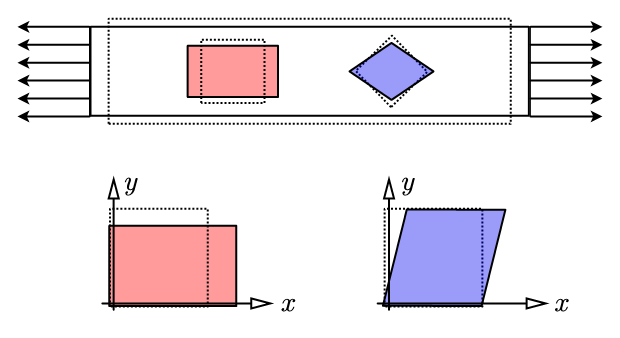
\includegraphics[width=7cm]{image/6-7-1.png}
\caption{正应变与剪应变}\label{6-7-1}
\end{wrapfigure}
其中三个对角元素$\varepsilon$称作\emph{正应变}(normal strain).\,而非对角的元素$\theta$称作\emph{剪应变}(shear strain).\,如图\ref{6-7-1}所示,\,在一种非常简单的模型中,\,大气中的棒被在沿棒方向施加一个拉力而伸长,\,但宽方向很自然地会产生些许的收缩.\,那么根据在棒里取出不同的微元形式,\,其变形方向也会有所改变.\,红色部分沿$x$方向就发生了明显的正应变.\,这是因为合适地平移,\,旋转其变形后的微元对齐形变前的微元(虚线)后,\,明显发现在$x$方向长度变大了.\,如果初始长度为$X$,\,之后在微元范围内端点的$x=X+\delta$.\,于是根据上面的定义,\,正应变其实就是:
\[\varepsilon=\frac{\delta}{X}=\frac{x-X}{X}\]

而蓝色部分是个平行四边形,\,将底边与变形前的底边对齐以后,\,我们发现$x-y$平面上顶角不再是$90^\circ$,\,这其实就标志着剪应变.\,如果这个角度减小了$\alpha$,\,那么之后的$x=X+Y\tan\alpha,\,y=Y$.\,这就说明$\delta_x=Y\tan\alpha,\,\delta_y=0$.\,从而:
\[\theta_{xy}=\frac{\partial \delta_y}{\partial X}+\frac{\partial \delta_x}{\partial Y}=\tan\alpha\approx \alpha\]

可见这个角度变化其实就是剪应变,\,它与边的对齐方式无关,\,如果$x,\,y$轴夹角变小便是正的.\,正应变,\,剪应变都是无量纲的物理量.

\vspace{0.5cm}

接下来需要考虑弹性体的内部受力情况.\,令人惊讶的是,\,它也必然由一个对称张量描述.\,首先我们意识到弹性力内部的受力具有以下特征:\,A.\,是空间点的函数,\,不同点处可以不同,\,但每一点应当有一个受力情况,\,它就是内部的\emph{应力}(stress).\,B.\,不是一个矢量.\,显然指出弹性体中的一点,\,并不能马上对应出来这个点处的某个受力的情况,\,因为我们考虑的是内力而不是外力,\,但是点处的受力不可能有明确的施力物体与受力物体.\,那么其实还需要在这一点处找到一个面矢量$\ud \bs{S}$,\,才能说是谁对谁的力.\,我们这样就发现了,\,其实指定一个应力,\,本质上就是在每一点指定一个面矢量$\ud \bs{S}$到相互作用力$\ud \bs{F}$的映射.\,C.\,显然,\,这样的映射应当为线性映射\footnote{证明留给读者做思考,\,需要用到极限微元受力分析.}.

\begin{wrapfigure}[15]{o}[-10pt]{7cm}
\vspace{-0.5cm}
\centering
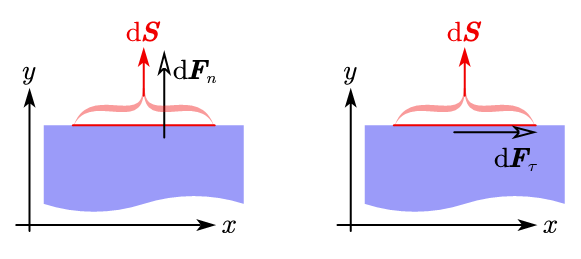
\includegraphics[width=7cm]{image/6-7-2.png}
\caption{正应力与剪应力}\label{6-7-2}
\end{wrapfigure}
这样就几乎已经说明,\,应力其实就是一个张量.\,因为从一个矢量$\ud \bs{S}$到另一个矢量$\ud \bs{F}$的线性映射的数学模型其实就是张量,\,它存在$3\times 3=9$个分量.\,我们进一步指定,\,$\ud \bs{F}$的含义$\ud \bs{S}$指向的那一侧的体元对这一侧的体元通过$\ud \bs{S}$施加的相互作用力.\,这个张量就是:
\[\left\{\begin{array}{ccc}\ud F_x &= & \sigma_{xx} \ud S_x + \sigma_{xy} \ud S_y+\sigma_{xz} \ud S_z \\ \ud F_y&= & \sigma_{yx} \ud S_x + \sigma_{yy} \ud S_y+\sigma_{yz} \ud S_z \\ \ud F_z &= & \sigma_{zx} \ud S_x + \sigma_{zy} \ud S_y+\sigma_{zz} \ud S_z \end{array}\right.\]
\[\bs{\sigma}:\; \ud \bs{S}\rightarrow \ud \bs{F}\]

\[\bs{\sigma}:\; \begin{bmatrix}\sigma_{xx}&\sigma_{xy}&\sigma_{xz}\\\sigma_{yx}&\sigma_{yy}&\sigma_{yz}\\\sigma_{zx}&\sigma_{zy}&\sigma_{zz}\end{bmatrix}\]

这个张量就叫做\emph{应力张量}(stress tensor).\,通过极限微元的受力分析,\,可以证明这个张量还必须是对称的\footnote{也留给读者自己完成.}.\,也就是说,\,我们可以写成以下形式:
\[\bs{\sigma}:\; \begin{bmatrix}\sigma_{x}&\tau_{xy}&\tau_{zx}\\\tau_{xy}&\sigma_{y}&\tau_{yz}\\\tau_{zx}&\tau_{yz}&\sigma_{z}\end{bmatrix}\]

同样的,\,参考图\ref{6-7-2},\,我们可以发现,\,对角线元素$\sigma$代表\emph{正应力}(normal stress)而非对角线元素$\tau$代表\emph{剪应变}(shear stress).\,如果把面元取为$\ud\bs{S}=\ud S_y\bs{e}_y$,\,考虑在平面上的受力就会产生两个分量:
\[\ud \bs{F}_n=\sigma_y \ud S_y\bs{e}_y\quad,\quad\ud \bs{F}_{\tau}=\tau_{xy} \ud S_y\bs{e}_x\]

前者就是垂直于面的以拉力为正的正应力,\,后者就是平行于面方向的剪应力.\,而应力本身都是和以往学过的压强量纲一致,\,国际单位是帕斯卡${\rm Pa}$:
\[\sigma=\frac{\ud F_n}{\ud S}\quad ,\quad \tau=\frac{\ud F_{\tau}}{\ud S}\]

\vspace{0.5cm}

引入两个张量以后,\,剩下的就是构造两者之间的因果关系:\,应力是如何造成应变的.\,在纯粹的弹性理论中,\,我们可以假设应力张量到应变张量的映射再一次是一个逐点线性的映射.\,这样的结果是数学上造成了每一点需要引入一个四阶的张量来描述这样的映射.\,三维情况下四阶的张量一共会造成$3^4=81$个独立分量.\,由于应力应变张量本身具有对称性,\,故其实只需要$6^2$个独立分量.\,再由于体系的非耗散性的要求\footnote{导致了某种形式互易定理.},\,其独立分量数最终减少到$21$个.\,这也是高度非对称的介质的弹性系数中独立的量的个数.\,然而,\,如果介质是完全各向同性的,\,也就是说沿所有三维空间中任意方向的长度与角度的拉伸与压缩都是相同困难的情况下,\,张量的对称性理论可以告诉我们,\,独立的弹性系数只会剩下两个.\,具体来说,\,$\bs{\varepsilon}$与$\bs{\sigma}$之间的关系必然会变成以下不依赖于坐标系选取的形式:
\[\bs{\sigma}=2\mu\cdot\bs{\varepsilon}+\lambda {\rm Tr}(\bs{\varepsilon})\cdot\bs{I}\]

而按照这样的方式选取的弹性系数$\lambda$和$\mu$被叫做\emph{拉梅参数}(Lam\'e parameters).\,式中${\rm Tr}$代表取迹操作,\,而$\bs{I}$是单位张量.\,带入之前的两个张量的写法上式实际上意味着:
\[\sigma_x=2\mu\varepsilon_x+\lambda(\varepsilon_x+\varepsilon_y+\varepsilon_z)\]
\[\sigma_y=2\mu\varepsilon_y+\lambda(\varepsilon_x+\varepsilon_y+\varepsilon_z)\]
\[\sigma_z=2\mu\varepsilon_z+\lambda(\varepsilon_x+\varepsilon_y+\varepsilon_z)\]
\[\tau_{ij}=\mu\theta_{ij}\]

至少我们能从上式发现,\,剪应力和正应力是分别独立地导致剪应变和正应变的,\,尤其是剪应力,\,它在三个方向甚至都是互相独立地,\,而这个比例系数就还被叫做\emph{剪变模量}(shear modulus),\,用$G$来表示.\,即拉梅系数$\mu\equiv G$.\,这个在切向成立的结论称作\emph{横向胡克定律}(transverse Hooke's law):
\[\frac{ F_\tau}{ S}=G \frac{ \delta}{ y}\]

而前三个式子对应的正应力正应变之间的关系比较复杂.\,首先我们把三式相加可以得到:
\[\sigma_x+\sigma_y+\sigma_z=(2\mu+3\lambda)(\varepsilon_x+\varepsilon_y+\varepsilon_z)\]\tabularnewline

我们意识到,\,任何物体在大气环境下实际上就受到周围分子不断撞击产生的大气压力而体积收缩,\,实际上就是三个方向应力相等于压强$\sigma_x=\sigma_y=\sigma_z=p$,\,而且三个应变$\varepsilon_i$就等价于线压缩率,\,应当是体压缩率的三分之一的情况,\,这样我们得到:
\[p=\left(\lambda+\frac{2}{3}\mu\right)\frac{\Delta V}{V}\]

这个系数就叫做\emph{体弹性模量}(bulk modulus):
\[K=\lambda+\frac{2}{3}\mu\]

一般来说,\,弹性体预先在大气体系中被压缩,\,在这个基础上,\,线性地叠加上由于其他形式的应力$\bs{\sigma}$导致的新应变$\bs{\varepsilon}$.\,

还有一种至关重要的变形.\,如果我们在一根弹性棒的$x$方向施加应力$\sigma$,\,但是$y-z$方向不施加任何的力$\sigma_y=\sigma_z=0$,\,扣除原来大气造成的应变,\,通过解方程得到$\varepsilon=\varepsilon_x$和$\varepsilon'=\varepsilon_y=\varepsilon_z$的值:
\[\left\{\begin{array}{ccc}\sigma &=&2\mu\varepsilon + \lambda(\varepsilon+2\varepsilon') \\ 0 &=&2\mu\varepsilon' + \lambda(\varepsilon+2\varepsilon')\end{array}\right.\Rightarrow\quad \left\{\begin{array}{ccc}\varepsilon &=& \frac{\lambda+\mu}{\mu(3\lambda+2\mu)} \sigma\\ \varepsilon' &=&-\frac{\lambda}{2(\lambda+\mu)}\varepsilon\end{array}\right.\]

第一个式子翻过来写就是描述拉力与棒伸长之间的\emph{纵向胡克定律}(longtitudinal Hooke's law).\,相关的弹性系数称作\emph{杨氏模量}(Young's modulus),\,即$E=\mu(3\lambda+2\mu)/(\lambda+\mu)$.\,而第二个式子反映了如果棒在拉力方向伸长,\,在垂直方向必然缩短的现实.\,缩短率与伸长率的比值称为\emph{泊松比}(Poisson's ratio),\,即$nu=\lambda/2(\lambda+\mu)$:
\[\frac{F_n}{S}=E\frac{\delta}{x}\quad ,\quad \frac{\delta'}{y}=\nu\frac{\delta}{x}\]

\begin{figure}[H]
\centering
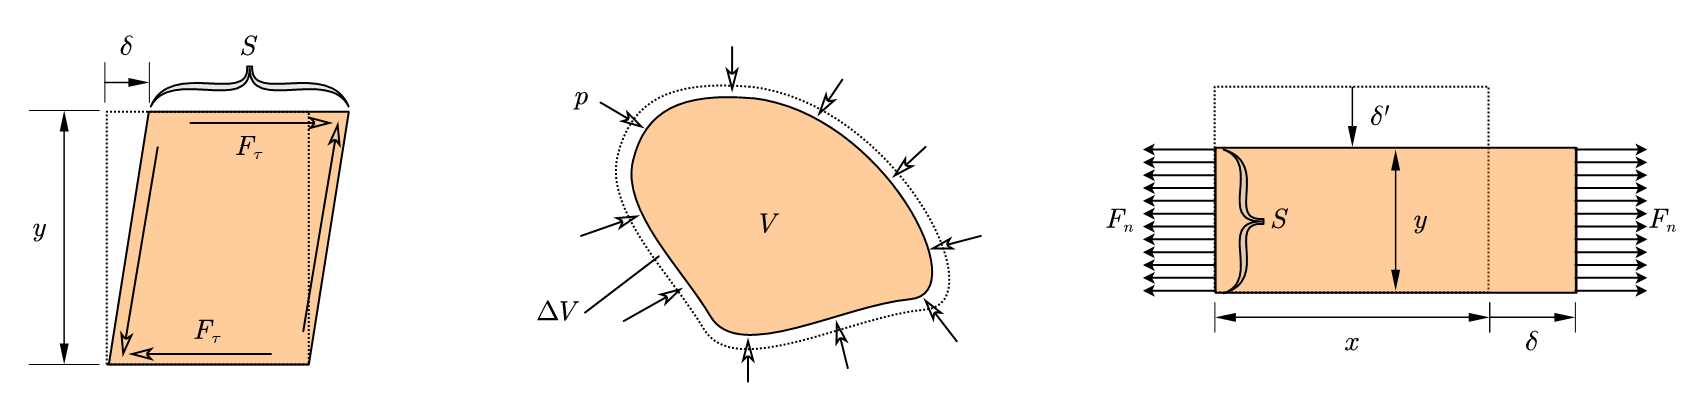
\includegraphics[width=14cm]{image/6-7-3.png}
\caption{剪变模量,\,体弹性模量与杨氏模量}
\end{figure}

三个弹性模量的单位也是应力的单位,\,即帕斯卡,\,而典型材料的弹性模量在$10^{10}{\rm Pa}$的数量级.


\section{弹性棒,\,弹性绳,\,弹性膜与弹性体}

\section{弹性波}


% %!TEX root = ../physical-olympics-2.tex
\chapter{流体}



\section{流体的物理描述}

\section{定常流动动力学}

\section{黏滞流体动力学}

\section{流体中的波}

\section{波的色散}
% %!TEX root = ../physical-olympics-2.tex
\chapter{相对论}


\section{相对论运动学}

\begin{itemize}
\item 光速不变原理:\,时空的结构为平直时空:\,$\text{d}s^2=c^2\text{d}t^2-\text{d}x_i^2$:\,物质运动的``舞台''.

\item 相对性原理:\,物理规律的协变性:
\[\text{Sca}.=\text{Sca}. \quad , \quad \text{Vec}.=\text{Vec}. \quad ,\quad  \text{Vec}.\cdot \text{Vec}.=\text{Sca}. \quad \text{etc}.\]

\item \emph{四-标量}(four-scalar)与\emph{四-矢量}(four-vector)的定义:\,类比三维空间标量矢量,\,但按闵可夫斯基空间处理.

\item 洛伦兹变换的定义:\,保度规的变换.\,物理上是不同共原点惯性参考者建立的参考系.

\item 洛伦兹群:
\[\text{SO}\left( 3,1 \right) =<R_x, R_y, R_z, B_x, B_y, B_z>\]

其中$B_x$为$x$方向的\emph{推促}(boost):
\[\left[ \begin{array}{c}
	ct\\
	x_1\\
	x_2\\
	x_3\\
\end{array} \right] ^{'} =\left[ \begin{matrix}
	\gamma&		-\gamma \beta&		0&		0\\
	-\gamma \beta&		\gamma&		0&		0\\
	0&		0&		1&		0\\
	0&		0&		0&		1\\
\end{matrix} \right] \left[ \begin{array}{c}
	ct\\
	x_1\\
	x_2\\
	x_3\\
\end{array} \right] \]

\item 经典物理没有协变性,\,但电磁学与相对论理论具有协变性.\,意为所有物理定律都由协变的对象构成,\,这主要包括标量,\,矢量,\,张量,\,旋量四类.\,四-矢量尤其常见:
\[\left[ \begin{array}{c}
	A_0\\
	A_1\\
	A_2\\
	A_3\\
\end{array} \right] ^{'} =\left[ \begin{matrix}
	\gamma&		-\gamma \beta&		0&		0\\
	-\gamma \beta&		\gamma&		0&		0\\
	0&		0&		1&		0\\
	0&		0&		0&		1\\
\end{matrix} \right] \left[ \begin{array}{c}
	A_0\\
	A_1\\
	A_2\\
	A_3\\
\end{array} \right] \]

出于方便,\,四-矢量也被简记为$A_{\mu}=\left( A_0, A_i \right) =\left( A_0, \boldsymbol{A} \right) $.\,而$A_i=\left( A_1, A_2, A_3 \right) $是三维矢量的简记.\,四-矢量与四-矢量可以算\emph{伪内积}(pseudo-inner-product):
\[A_{\mu}B^{\mu}=A_0B_0-A_iB_i\]

伪内积将得到四-标量.\,即参考系变换下不变的量.

\item 洛伦兹变换下任意四-矢量具有不变量$A_{\mu}A^{\mu}=A_{0}^{2}-\boldsymbol{A}^2$,\,对于类时四-矢量这将大于零,\,即$A_{\mu}A^{\mu}=A_{\text{proper}}^2$,\,事实上以速度$\boldsymbol{v}=\frac{\boldsymbol{A}}{A_0}c$做洛伦兹变换,\,可以把空间分量变为零.\,这叫做\emph{本征参考系}(proper reference system).\,得到本征四-矢量$A_{\mu}'=\left( A_{\text{proper}}, \mathbf{0} \right)$.

\item 三个基本图像:

\begin{itemize}
\item 尺缩:\,$L=L_0/\gamma$.

\item 钟慢:\,$t=\gamma t_0$.

\item 同时相对性:\,$\tau=-\beta \frac{x}{c}$.

\end{itemize}

只要是真的尺子,\,真的钟,\,就永远不可能错!\,没有真的尺子和钟就去构造.

\item 相对论质点运动:

具有四-标量:\,间隔$\text{d}s=\sqrt{\text{d}x_{\mu}\text{d}x^{\mu}}$,\,本征时$\ud t_0=\ud s/c$,\,下四-速度的不变模长$v_\mu v^\mu=c^2$.

具有四-矢量:\,四-位移$\text{d}x_{\mu}=\left( c\text{d}t, \text{d}\boldsymbol{r} \right) $,\,四-速度$v_{\mu}=\left( \gamma c, \gamma \boldsymbol{v} \right) $,\,四-加速度见下节.

\item 速度变换公式:

$$
\gamma '=\frac{1-\frac{uv_x}{c^2}}{\sqrt{1-u^2/c^2}}\gamma 
$$

$$
v_x'=\frac{v_x-u}{1-\frac{uv_x}{c^2}}
$$

$$
v_{y,z}'=\frac{\sqrt{1-u^2/c^2}}{1-\frac{uv_x}{c^2}}v_{y,z}
$$

\item 光行差公式:\,可以用速度变换推导,\,也可以之后用流变换推导:
\[\cos \theta'=\frac{\cos \theta -\beta}{1-\beta \cos\theta}\quad ,\quad \sin \theta'=\sin\theta\cdot \frac{\sqrt{1-\beta^2}}{1-\beta \cos\theta}\quad ,\quad \tan\theta =\frac{\sin \theta'}{\cos \theta'}\]

\item 相对论下讨论刚体?\,模型存在缺陷:\,隧道佯谬,\,转盘佯谬.\,故整个刚体运动学都没有必要建立.

\end{itemize}

\section{相对论动力学}

\begin{itemize}
\item 动量-能量构成四矢量的必要性:\,守恒律需要被保留且协变.

\item 四-动量:
\[p_{\mu}=\left( \frac{E}{c}, \boldsymbol{p} \right) \,\,, p_{\mu}p^{\mu}c^2=E^2-p^2c^2=m^2c^4\,\,, \boldsymbol{v}=\frac{\boldsymbol{p}c^2}{E}\]

\[\boldsymbol{p}=\frac{m\boldsymbol{v}}{\sqrt{1-v^2/c^2}}\,\,, E=\frac{mc^2}{\sqrt{1-v^2/c^2}}\]

\item 普遍的过程的守恒律:
\[\sum_i{p_{i,\mu}}=\sum_j{p_{j,\mu}}\]

\item 四-力与四-加速度:
\[a_{\mu}=\frac{\text{d}v_{\mu}}{\text{d}t_0}=\left( \gamma \frac{\text{d}\gamma}{\text{d}t}c, \gamma \frac{\text{d}\gamma \boldsymbol{v}}{\text{d}t} \right) \,\,, \frac{\text{d}\boldsymbol{v}}{\text{d}t}:=\boldsymbol{a}\]

\[F_{\mu}=\frac{\text{d}p_{\mu}}{\text{d}t_0}=\left( \gamma \frac{\text{d}E}{c\text{d}t},\gamma \frac{\text{d}\boldsymbol{p}}{\text{d}t} \right) :=\left( \gamma \frac{W}{c},\gamma \boldsymbol{F} \right) \]

\begin{itemize}
\item 推论一:\,$F_\mu=a_\mu$.\,但三维矢量之间不会直接符合Newton-like的动力学方程.

\item 推论而:\,$F_\mu v^\mu=0$.\,这个三维继续可以得到:
\[\boldsymbol{F}\text{d}t=\text{d}\boldsymbol{p}\,\,, \boldsymbol{F}\cdot \text{d}\boldsymbol{r}=\text{d}E\]
\end{itemize}

\item 单方向受力时,\,在该方向的推促下力不变.

\item 本征加速度与本征力:\,它本意指的是\emph{四-速度的本征系}中的四-加速度与四-力,\,不过神奇的是恰好让两者的时间分量变为零(类空,\,与类时的四-速度正交),\,空间分量为$\bs{a}_0,\,\bs{F}_0$:
\[\bs{F}_0=m\bs{a}_0\]
\[a_\mu a^\mu=-a_0^2\]

\item 沿平行于本征加速度与本征力方向施以推促:
\[F=F_0\quad ,\quad a=a_0/\gamma^3\]

\item 沿垂直于本征加速度与本征力方向施以推促:
\[F=F_0/\gamma\quad ,\quad a=a_0/\gamma^2\]

\item \emph{快度}(rapidity):\,$\beta={\rm th} \vartheta,\,\gamma={\rm ch} \vartheta$.

\item 自然坐标下的相对论性牛顿定律:
\[F_\tau=\gamma^3 ma_\tau\]
\[F_n=\gamma ma_n\]

\item 相对论关于碰撞的新理解:

\begin{table}[H]
\centering
\begin{tabular}{c|c|c}
\hline
情形 &经典 & 相对论\\\hline
弹性 & 无耗散,\,$\bs{p}'=\bs{p},\,E'=E$ &粒子守恒,\,$\bs{p}'=\bs{p},\,E'=E$\\\hline
非弹性 & 有耗散,\,$\bs{p}'=\bs{p},\,E$不可列 &粒子变性,\,$\bs{p}'=\bs{p},\,E'=E$\\\hline
\end{tabular}
\end{table}

只有一个例外:\,光子的散射若频率不变,\,叫做弹性散射.\,如经典的瑞利散射,\,米氏散射;\,但如果频率变了,\,叫做非弹性散射,\,如拉曼散射,\,康普顿散射.

\item 相对论碰撞根据具体情形一般有以下大的分类:\,弹性的散射,\,非弹性的散射,\,粒子反应.

\item 质点系的动量-能量也将构成一个四-矢量,\,即:
\[(E,\,\bs{p})=\sum_i (E_i,\,\bs{p}_i)\]

那么这个四-矢量的本征系速度:
\[\bs{v}=\frac{\bs{p}c^2}{E}\]

称作\emph{动量中心系}(center-of-momentum frame),\,以代替经典物理的质心系.\,简称动心系.\,顾名思义,\,此系中质点系总动量为零:\,而总能量:
\[E_0^2=E^2-\bs{p}^2c^2=m_0^2 c^4\]

$m_0$为动心系中的总动质量,\,以后称作质点系的等效静质量.\,这个式子可以解释一部分的质量起源问题.

\item 一个等效静质量$m_0$的质点系若选取相对动心系以$\bs{v}$运动的参考系,\,动量与能量为:
\[\bs{p}=\sum_i \bs{p}_i =\frac{m_0\boldsymbol{v}}{\sqrt{1-v^2/c^2}}\]
\[E=\sum_i E_i=\frac{m_0 c^2}{\sqrt{1-v^2/c^2}}\]

\item 放能反应:\,$\sum_i m_i>\sum_j m_j$.\,则无论取哪个系,\,静能转化为动能的量都相等.\,定义为反应能$Q$:
\[Q=\left(\sum_i m_i-\sum_j m_j\right)c^2\]

\item 吸能反应:\,$\sum_i m_i<\sum_j m_j$.\,则具有阈能.\,\emph{仅在动心系中},\,反应发生的最小动能(阈能)的值为:
\[Q=\left(\sum_j m_j-\sum_i m_i\right)c^2\]

\end{itemize}
	
\section{相对论连续物质}

\begin{itemize}
\item 若有一守恒荷$Q$作为四-标量,\,则其空间分布与流动构成一个密度场$\rho,\,\bs{j}$:
\[\ud Q=\rho\ud V\]
\[\ud Q=\bs{j}\cdot \ud \bs{S} \ud t\]

\item 那么$(\rho c,\,\bs{j})$是一个四-矢量且符合洛伦兹变换,\,如$x$方向的推促:
\[\left[ \begin{array}{c}
	\rho^{'}c\\
	j_x^{'}\\
	j_y^{'}\\
	j_z^{'}\\
\end{array} \right]  =\left[ \begin{matrix}
	\gamma&		-\gamma \beta&		0&		0\\
	-\gamma \beta&		\gamma&		0&		0\\
	0&		0&		1&		0\\
	0&		0&		0&		1\\
\end{matrix} \right] \left[ \begin{array}{c}
	\rho c\\
	j_x\\
	j_y\\
	j_z\\
\end{array} \right] \]

\item 若有一平面波场,\,其必要的一个要素为相位,\,它随着时空分布必然写作:
\[\varphi=\omega t-\bs{k}\cdot\bs{r}\]

$\omega$称作角频率,\,$\bs{k}$为波矢.

\item 那么由于相位为四-标量,\,且可以写作以下形式,\,故$k_\mu=(\omega/c,\,\bs{k})$为四-矢量,\,称作四-波矢:
\[\varphi=k_\mu x^\mu\]

如$x$方向的推促:
\[\left[ \begin{array}{c}
	\omega^{'}/c\\
	k_x^{'}\\
	k_y^{'}\\
	k_z^{'}\\
\end{array} \right]  =\left[ \begin{matrix}
	\gamma&		-\gamma \beta&		0&		0\\
	-\gamma \beta&		\gamma&		0&		0\\
	0&		0&		1&		0\\
	0&		0&		0&		1\\
\end{matrix} \right] \left[ \begin{array}{c}
	\omega /c\\
	k_x\\
	k_y\\
	k_z\\
\end{array} \right] \]

\item 可以从上式出发得到光行差公式,\,同时也能得到多普勒效应公式.\,在前提$\omega/k=c$(四-波矢类光)时:
\[\omega'=\omega\cdot \frac{1-\beta \cos\theta}{\sqrt{1-\beta^2}}\]

\[\cos \theta'=\frac{\cos \theta -\beta}{1-\beta \cos\theta}\]

\item 将三维的力密度和功率密度:
\[\bs{f}=\frac{\ud \bs{F}}{\ud V}\]
\[p=\frac{\ud P}{\ud V}\]

合并可以得到四-力密度$f_\mu=(p/c,\,\bs{f})$.

\end{itemize}

\section{相对论电磁场}

相对论场变换公式:
\[E_{//}'=E_{//}\quad ,\quad B_{//}'=B_{//}\]
\[\bs{E}_\perp'=\frac{\bs{E}_\perp+\bs{v}\times \bs{B}_\perp}{\sqrt{1-\beta^2}}\quad,\quad \bs{B}_\perp'=\frac{\bs{B}_\perp-\bs{v}\times \bs{E}_\perp/c^2}{\sqrt{1-\beta^2}}\]

%!TEX root = ../physical-olympics-2.tex
\chapter{热力学第一定律}


\section{热力学第零定律}
热力学系统的状态可以分为\emph{平衡态}(equilibirium state)和\emph{非平衡态}(non-equilibrium state).\,平衡态这样一种状态,\,首先它是一种宏观性质都不随着时间演化的状态---稳定态\footnote{注意,\,一是从微观上看,\,组成系统的微观粒子仍然处于无休无止的运动中,\,其微观坐标与速度在发生几急剧的变化,\,但平衡态只对宏观性质定义.\,二是统计力学可以证明,\,处于平衡态的系统总是由于内在随机性而产生涨落,\,有时甚至不可忽略,\,如临界乳光现象.\,这说明我们的平衡态模型只能是一种近似,\,实际情况往往还有很多需要考虑的因素.},\,但稳定态不一定是平衡态,\,如两端温度保持不变后稳定导热的杆,\,如稳定喷气的火箭,\,如不断气化液化工作循环制冷的空调工作物质.\,原因是它们没有符合以下三个平衡条件:
\begin{description}
	\item[\quad \quad {\CJKfamily{hei} 热学平衡}]	系统各部分温度严格相等.
	\item[\quad \quad {\CJKfamily{hei} 力学平衡}]	系统内力(如压强)与外力达到平衡,\,如重力场下的等温大气模型.
	\item[\quad \quad {\CJKfamily{hei} 化学平衡}] 	系统各部分热运动扩散的趋势相互平衡,\,如饱和糖水与糖块共存.
\end{description}

可以发现,\,既使系统状态不均匀,\,如重力场等温大气模型的各处压强和饱和糖-糖水模型中的两相糖分子数密度,\,系统也是处于平衡态的.\,而如果这些平衡条件没有达成,\,系统内部将发生各种宏观可见的\emph{输运过程}(transport phenomena).\,如温度不均导致的热传导,\,速度与压强不均导致的黏滞,\,及浓度不均导致的扩散.\,不平衡的力产生了不平衡的流,\,相应的研究是非平衡态物理研究的对象.\,这种情况下既使系统随时间稳定,\,也不是平衡态.

上文中已多次提及\emph{温度}(temperature)这一物理概念.\,今天的我们完全可以用统计力学的思考方式来理解它:\,诚然,\,{\CJKfamily{hei} 温度是分子热运动剧烈程度的量化}.\,如理想气体的温度定义为:
\[T=\frac{2\overline{\varepsilon_k}}{3k}\]

其中$\overline{\varepsilon_k}$表示分子平均\emph{平动}动能,\,而$k$表示玻尔兹曼常数.\,也就不难理解,\,为什么温度不均将导致传热,\,因为分子平均动能大的子系统$\mathrm{A}$与分子平均动能小的子系统$\mathrm{B}$发生热接触时,\,平均效应是$\mathrm{A}$中的分子通过相互作用要把能量给$\mathrm{B}$.\,这叫\emph{热传递}(heat transfer).

然而,\,在统计力学还没有诞生前,\,甚至在很长的一段时间内人们对热与温度的能量本质并没有明确的认识,\,\emph{热质说}(caloric theory)大行其道,\,人们把热量导致的温度升高视为与功导致的能量升高为完全独立的两个维度.\,但正是在这样的环境内,\,诞生了基于经验规律的物态方程,\,发明了测温,\,量热的各种实用仪器,\,乃至甚至产生了公理化的热力学体系.\,热力学第零定律即给出了温度可定义的依据.
\begin{description}
	\item[\quad \quad {\CJKfamily{hei} 热力学第零定律}]		任意两个各自达到热平衡的系统若发生热接触可以直接形成热平衡,\,则说这两个系统具有一致的温度.\,等温具有反身性,\,交换性与传递性.
	\item[\quad \quad {\CJKfamily{hei} 热力学第零定律的补充}]		如果两个各自达到热平衡的系统若发生热接触一者传递给另一者热量,\,则说前者比后者温度高.
\end{description}

这一定律确定了温度作为系统的\emph{态函数}(state function),\,它能像一个数那样可以进行大小的比较.\,有两点值得注意:

一是热力学第零定律定义了温度,\,但它没有量化一个\emph{温标}(temperature scale).\,如何量化一个温标呢?\,从各种系统平衡态的性质出发可以以某一具有特点的状态量作为温度评价的标度.\,如理想气体温标,\,黑体辐射谱温标和噪声温标等等.\,而我们发现,\,温度高低的比较似乎与其传热的难易程度有关,\,是否可以利用这一点自然而然地定义普适温标呢?\,热力学第二定律回答了这个问题,\,答案是肯定的.

二是热力学第二定律与热力学第零定律的内在联系.\,作为热力学第零定律的补充,\,其实它正是热力学第二定律的一部分.\,热力学第二定律中得到了很好的量化定义了热力学温标以完善温度这一概念.\,其实,\,这两个定律的背后是简单的统计规律,\,若我们采取一种统计力学的方法,\,我们的理论基础便是统计公设,\,而热力学定理反而成为我们需要去证明和解释的对象了.








\section{热力学第一定律}

热力学第一定律的研究对象是热力学过程,\,是既定系统连续发生的这样或那样的真实状态改变.\,而热力学第一定律的微观本质是普遍的能量转化与守恒原理.\,它写为:
\[\ud U=\dbar W+\dbar Q\]

$U$为系统内能,\,表示系统内部能量的总和.\,等式左边为内部能量增量,\,右边为外界输入系统内部的能量,\,其中$\dbar W$为外界对系统内部的做功,\,而$\dbar Q$为外界通过热接触,\,以微观碰撞交换能量的形式,\,产生的平均宏观能量输送的大小.\,注意,\,$U$前面的$\ud$,\,表示无穷小变化量,\,但$W$与$Q$前面的$\dbar$,\,仅仅表示无穷小量(微元),\,不是某个热力学态函数的微分.\,这也是两个微分符号记法不相同的原因.\,这两种不同的热力学量可以称为\emph{状态量}(state quantity)与\emph{过程量}(process quantity).

在具体考察上述三个量的具体范围前,\,明确一下过程发生的具体形式是十分有必要的.


\subsection{准静态与非准静态过程}
\emph{准静态过程}(quasi-static process):\,过程进行地速度无限缓慢,\,以至于每一时刻系统都几乎处于平衡态.\,如等温传热的过程;\,保持外界压强始终等于气缸压强地压缩气体的过程;\,亦或是缓慢地冷却热溶液,\,使得溶质析出的过程,\,都是准静态过程.\,相反,\,高温物体向低温物体放热的过程,\,气体向真空自由膨胀的过程,\,把糖丢进纯水里溶解的过程或两种不同气体混合的过程,\,就都是非准静态过程.

过程的准静态与非准静态有以下两个特征:

一是准静态由于每时每刻都是平衡态,\,所以可以由平衡态的均匀状态参量去描写,\,从而得出各状态参量随时间的变化关系,\,消去时间可得\emph{状态方程}(process equation).\,更特别地,\,在过程中所发生的内能变化,\,做功,\,吸热全都可以用状态方程去确定,\,比如以$p,\,V$作为状态参量的理想气体:
\[\ud U=\frac{\partial U}{\partial p}\ud p + \frac{\partial U}{\partial V}\ud V \quad ; \quad \dbar W =-p\ud V \quad ; \quad \dbar Q=\ud U-\dbar W \]

注意在上式中最后一式不是说$\dbar Q$是$\ud U$与$\dbar W$的结果,\,在热一的公式中,\,等式右边的做正负功和吸放热永远是原因,\,等式左边内能的增减永远是结果.\,不过这是一个很常用的计算式,\,图像也还算直观:\,气体吸收的热量用来增加内能和对外做功.

而非准静态过程则不能由状态方程描写,\,也没有以上三个方程的成立,\,我们在更晚些时候展开讨论.

二是准静态过程由于每时每刻都达到了平衡,\,在平衡的状态下发生热量,\,功或者粒子的交换,\,所以是可逆过程\footnote{严格地说,\,还要求过程没有耗散,\,耗散是一类功变热的行为,\,它使得有序的功对应的能量转化为无序的热对应的能量.}.\,而由于非准静态过程没有达到各种平衡,\,故自发产生的各种过程都是不可逆的.

我们接下来仔细考虑内能,\,功与热量三个物理概念.


\subsection{内能}
\emph{内能}(internal energy),\,就是系统内部的能量和.\,它由许多可能的成分构成,\,如:
\begin{description}
	\item[\quad \quad {\CJKfamily{hei} 分子平动动能}]		三个自由度;
	\item[\quad \quad {\CJKfamily{hei} 分子转动动能}]		线性分子只有两个自由度\footnote{分子对自转轴的转动不会带来系统的改变,\,这与全同粒子的量子本性有关系.};\,非线性分子则有三个;
	\item[\quad \quad {\CJKfamily{hei} 分子振动动能}]\footnote{注意由于量子效应,\,室温下振动能量可以认为不被激发.}		分子间键长,\,键角偏离平衡位置的集体振动模式,\,其自由度数与上两者之和为$3n$,\,$n$为分子含原子数;
	\item[\quad \quad {\CJKfamily{hei} 分子振动势能}]		由于分子的振动,\,其势能也会比其平衡位置更大,\,近似地与分子振动动能相等;
	\item[\quad \quad {\CJKfamily{hei} 键能}]				即电子运动的动能势能之和(全部能量);
	\item[\quad \quad {\CJKfamily{hei} 静能}]				这里指以上运动的动能,\,势能全部去除后,\,由于更加深层次内部相对运动造成的静能量,\,如核能,\,基本粒子的自能等等.
\end{description}

有两点值得注意:

一是在内能具体的计算中,\,对于我们不关心的,\,过程中不发生改变的部分我们将其置零.\,如双原子分子理想气体的问题中研究的内能不会去包括两原子间化学键的能量,\,除非发生化学反应.\,而在常温下其振动自由度往往难以被激发,\,故其等效自由度约为$5$.\,自然界对于尺度的放缩并不具有对称性,\,所以很多能量实际上在更微小的层次内封装为不变的整体,\,这使得我们只需要研究我们关心的尺度上的问题,\,即\emph{有效理论}(effective theory)的思想.

二是有一些形式的能量是否属于内能的一部分视问题的不同而可以做不同的处理.\,这体现为功能原理上:
\[\dbar W_{\rm conservative}=-\ud E_{\rm potential}\]

即,\,在热力学第一定律的计算中,\,我们不去计算保守力部分做的功.\,而是把它对应的势能视为系统内能的一部分:
\[\ud U=\dbar W_{\rm others} + \dbar W_{\rm conservative} +\dbar Q \quad \Longrightarrow \quad \ud U_{\rm total}=\ud U + \ud E_{\rm potential}=\dbar W_{\rm others}+\dbar Q\]

最经典的例子是那些热力学系统中每个粒子都具有外场中的相互作用势能的情况.\,如气体的重力势能与电介质的静电能,\,就常常当做系统内能的一部分,\,然而有些情况下又使用不含这些能量的系统内能更加方便.\,再比如在恒定的外压强下的气体系统,\,外界对气体做功可以用体积功来表示:
\[W=\int_{V}^{V+\Delta V} \!\!(-p_0 \ud V)=-p_0 \Delta V\]

从中可以看出,\,气体具有体积能$E_{\rm volume}=p_0 V$,\,可以定义新的总内能为:
\[H_0=U+p_0 V\]

如果气体与外界压强平衡\footnote{如系统在大气压下发生一个化学反应等等.},\,则上式中的压强就是气体压强$p$,\,以上量称为气体的\emph{焓}(enthalpy):
\[H=U+pV\]


\subsection{功}
\emph{功}(work)有两个特点:\,一,\,功是一种能量转移,\,考虑功能原理,\,对一个系统做正功使得系统动能增加,\,而这是系统内能的一部分,\,从而能量传入系统.\,二,\,功总是与力对应. 热力学中为了方便我们引入所谓\emph{广义力}(generized forces)与\emph{广义坐标}(generized coordinates)来方便表示我们的系统. 如理想气体广义坐标如果取做体积$X=V$,\,则广义力就是外压强的相反数$Y=-p_0$,\,它们满足外界对研究的系统做功为:
\[\dbar W=Y\ud X=-p_0\ud V\]

这被叫做\emph{体积功}(volume work).\,与其他形式的功对应的广义力与广义坐标并在一张表中供参考:
\begin{figure}[H]
\centering
\begin{tabular}{c|c|c}
\hline
功形式		&	广义力					&	广义坐标			\\ \hline\hline
体积功		&	$-p$ 				&	$V$ 			\\ \hline
表面张力功  &	$\sigma$    		&   $S$ 		    \\ \hline
电路功		&   $U$ 				&   $Q$				\\ \hline
极化功		&	$E$ 				&  	$P$ 			\\ \hline
磁化功		&	$H$ 				& 	$M$ 			\\ \hline
\end{tabular}
\end{figure}

\begin{wrapfigure}[14]{o}[-10pt]{7cm}
\centering
\vspace{-30pt}
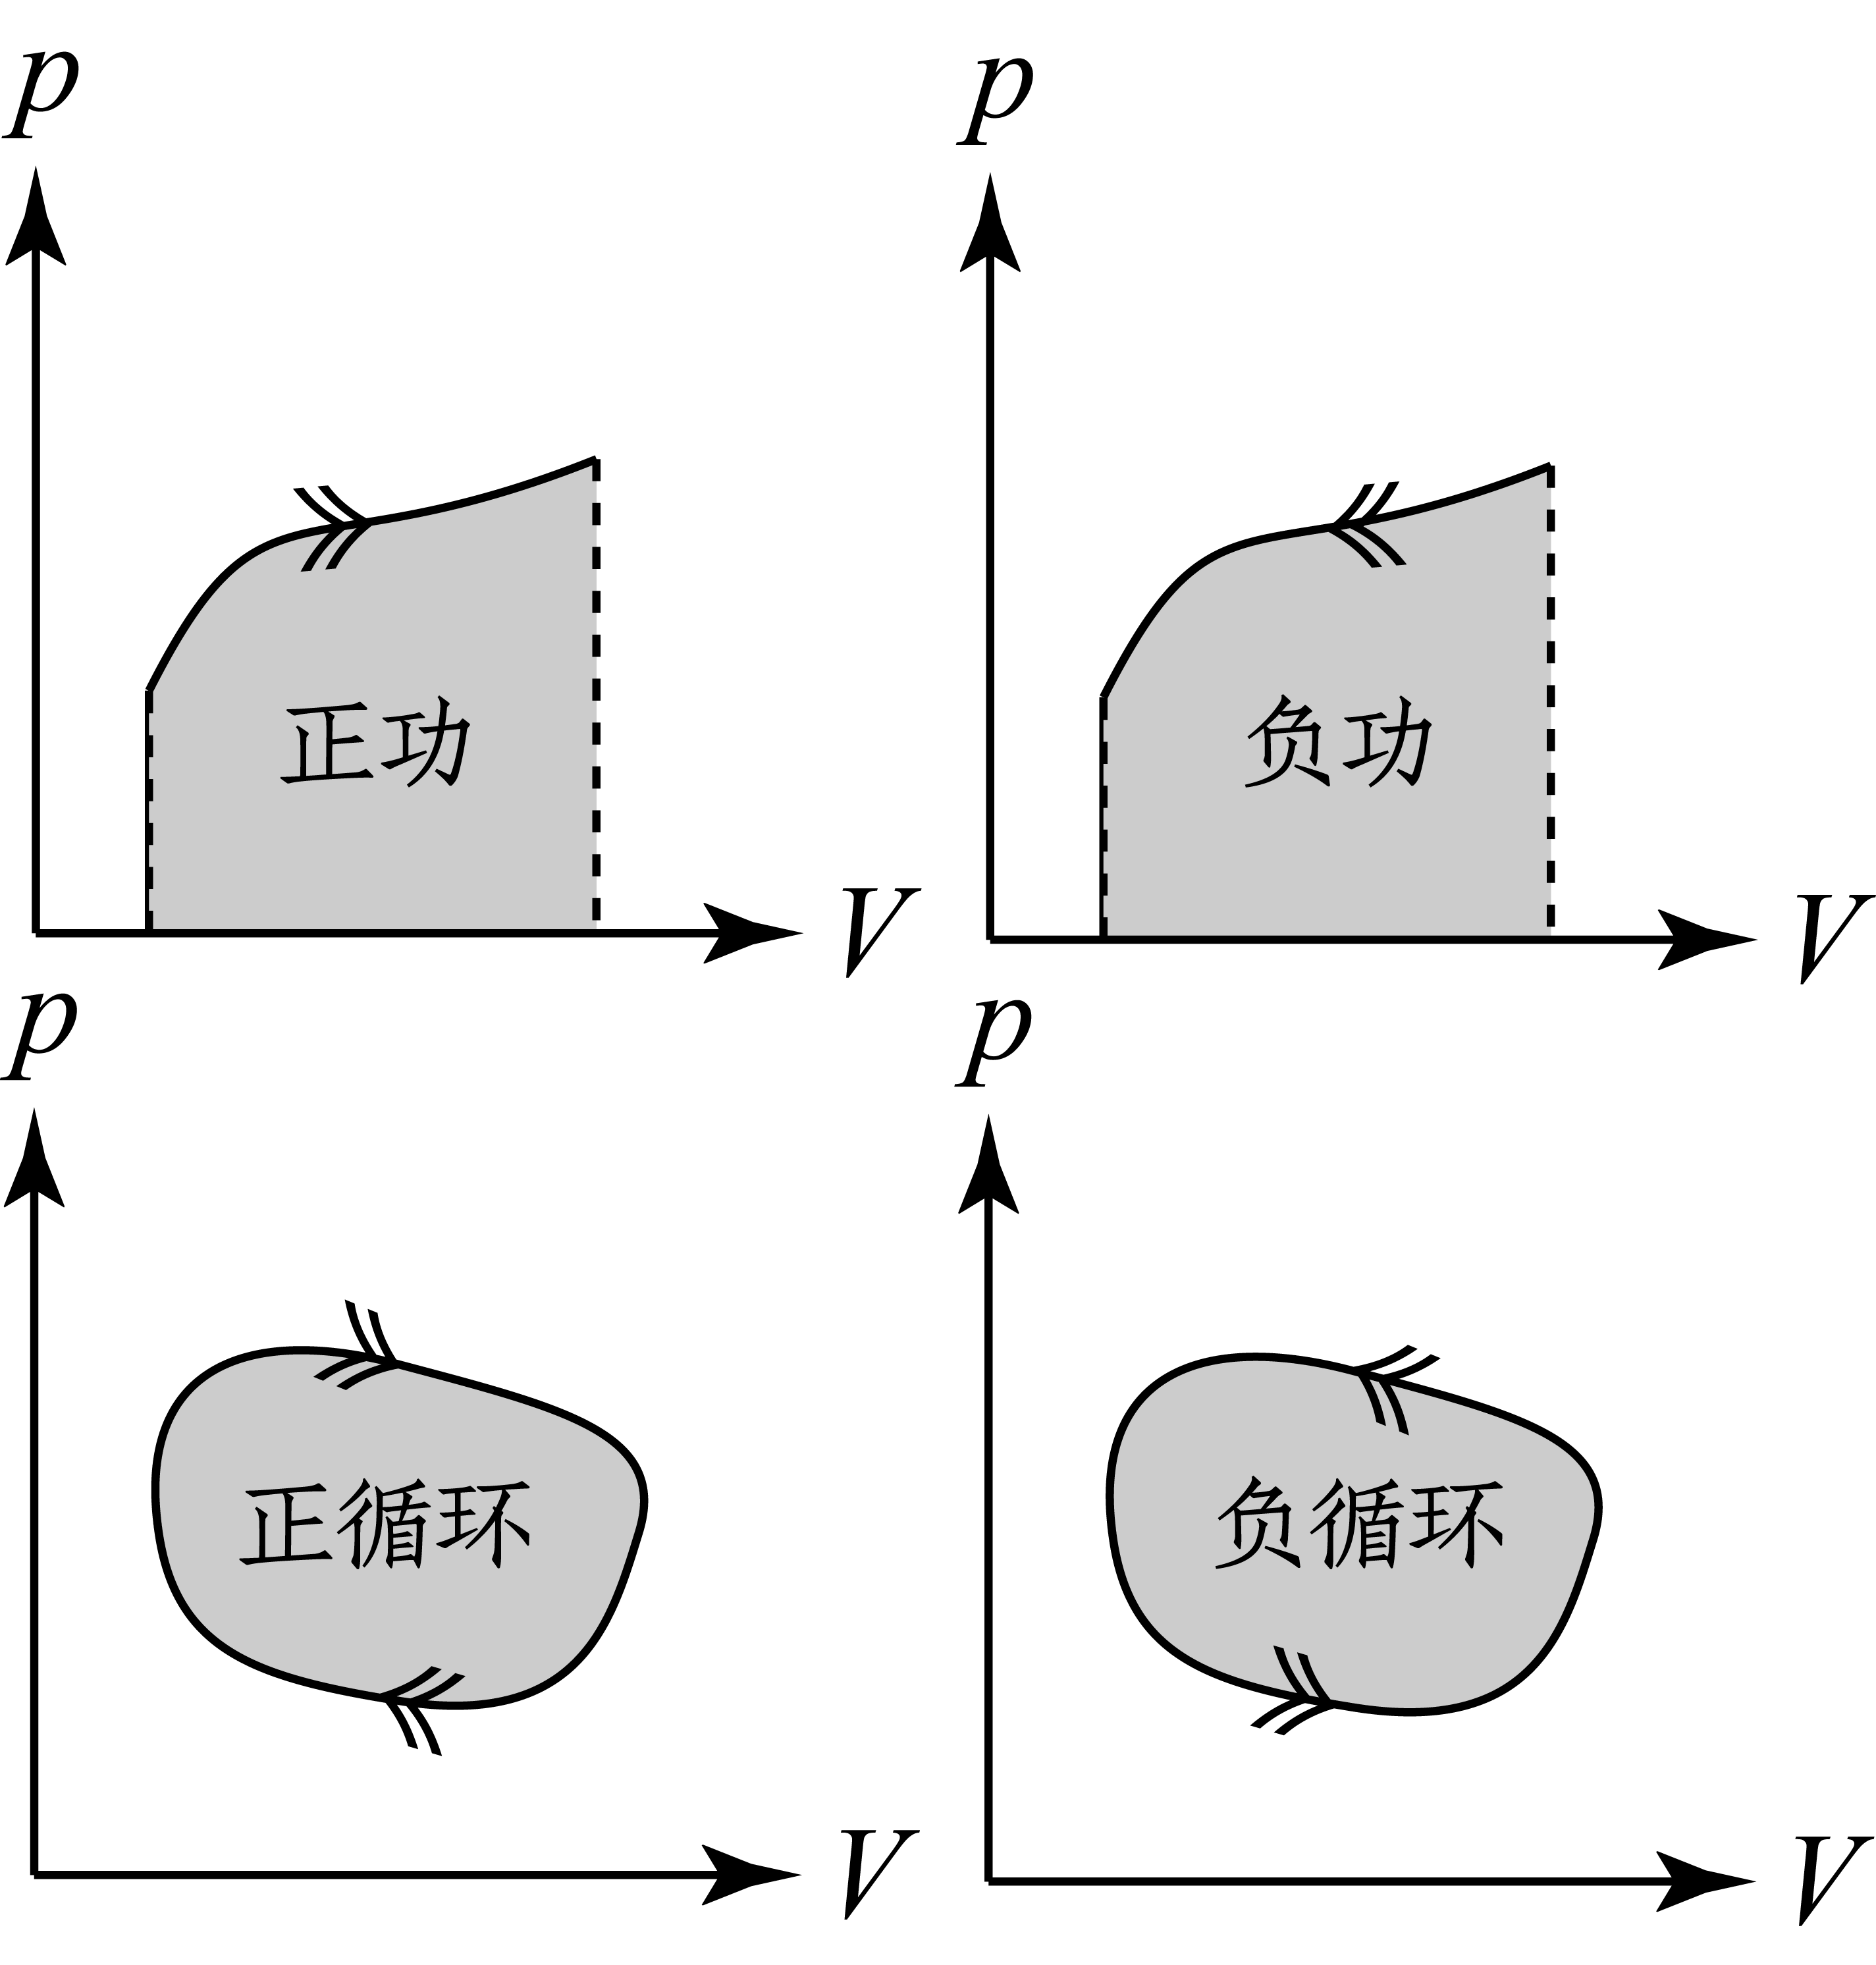
\includegraphics[width=7cm]{image/5-1-1.png}
\caption{准静态过程的做功}
\end{wrapfigure}
对于体积功,\,在准静态过程中可以由$p-V$图下的面积计算.\,在循环过程中则等于过程曲线所包含的面积.\,注意其正负号与过程方向之间的关系.\,但对于非准静态过程.\,做功一定要由外界参数(活塞加速度,\,活塞外气压等)计算而不是用内部气体的过程方程.\,这是因为即使形式地写出内部气体所发生的过程的过程方程.\,由于气体发生膨胀处的压强不等于过程方程中的平均压强,\,对做功的计算是没有意义的.
\subsection{热量}
做功与\emph{传热}(heat transfer)是截然不同的两种向系统注入能量的方式.\,做功依赖于广义坐标这一参数的改变.\,本质上与每一个微观粒子的能量对于广义坐标的依赖有关.\,然而热量则完全不依赖于外在的参数.\,它与系统粒子关于不同能量的状态的占据数\emph{配分}(partition)有关.\,也就是与温度息息相关.\,温度高的物体,\,占据在高能量状态上的粒子较多,\,低能量状态的粒子较少,\,与低温物体发生热接触时,\,单位时间内高能粒子碰撞低能粒子传递能量的可能性更高.\,其统计平均效应就是高温物体向低温物体放热.\,准静态的\emph{等温传热}又是怎样一个过程呢?\,从以上分析可知,\,产生温度梯度是有热传导\footnote{注意,\,广义的热量传递还包括热对流与热辐射.}的必要条件,\,没有了温度差热量的交换也就无从谈起了.\,从这个意义上说,\,实际发生的过程其实都是非准静态过程,\,准静态过程仅仅是一种实际过程的一种近似.\,或是我们虚设的一种模型.\,如在等温传热模型中,\,我们设想只让一个物体的高能粒子与另一个物体的低能粒子发生热接触而实现热传递,\,这无疑会破坏热力学的统计规律\footnote{或是借助于所谓的麦克斯韦妖,\,引入信息熵.},\,但有助于我们理解这个过程的发生机理.

\npg{-10pt}

\subsection{耗散}
\begin{wrapfigure}[14]{o}[-10pt]{7cm}
\centering
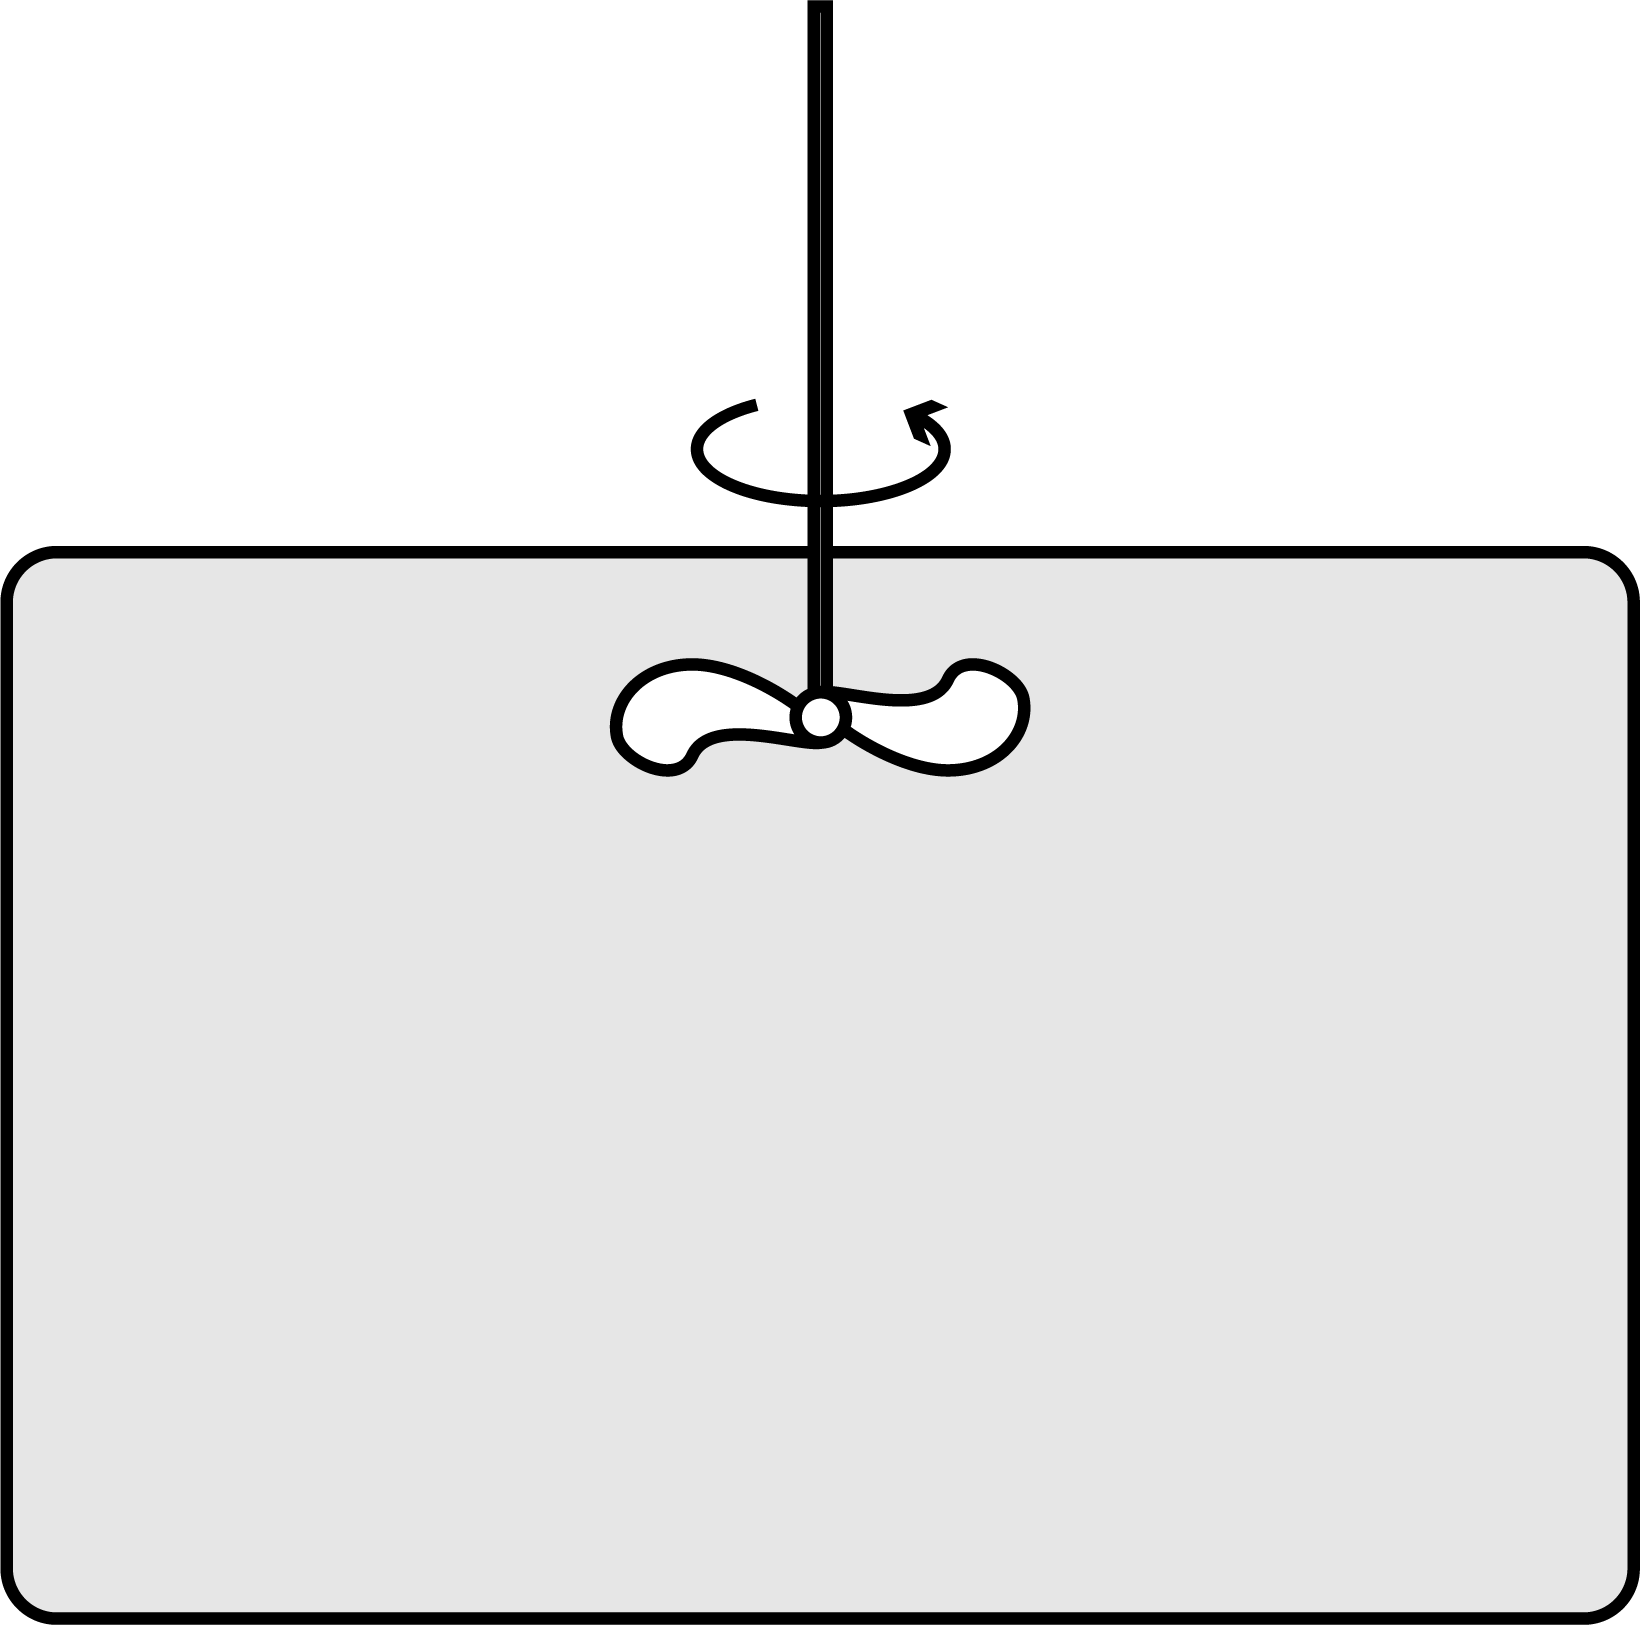
\includegraphics[width=6cm]{image/5-1-2.png}
\caption{搅动空气发热}\label{fig:1-2}
\end{wrapfigure}
还有一类向系统输送能量的方式,\,表面上看是功,\,效果上却是热.\,这被我们称为\emph{耗散}(dissipation).\,俗称\emph{功变热}.\,例如常见的摩擦生热过程,\,非弹性碰撞的过程,\,激光泵浦的过程.\,都是典型的功变热的例子.\,我们看一个十分浅显的例子.\,涡轮叶片搅动气缸中的空气使其温度升高.\,在这个过程中,\,涡轮无疑对气体做功,\,但这个做功并不与系统广义坐标的变化相关.\,它的特点是仅仅作用在系统的一个子系统上.\,再由系统倾向于热平衡的趋势把得来的能量平分到系统各个自由度上.\,从而造成了与吸热完全类似的结果:\,广义坐标没有变化,\,但系统从外界获得了能量.

究其原因,\,本质上是因为系统具有了所谓的\emph{耗散结构}(dissipative structure).\,它不把系统看成一个平衡的整体,\,而是有着复杂内部非线性相互作用的对象.\,故输入的功不一定改变体系的广义坐标,\,但像加热一个系统一般,\,增加了系统的内能.

耗散结构的特点之一是外力驱动系统远离平衡态.\,在非弹性的碰撞过程中固体内部的低频弹性波的成分被突然增强,\,而激光发射的过程中大量粒子被输运到亚稳态而实现布居反转,\,这些都破坏了原来热平衡下的布局.\,需要结合动力学与统计方法来讨论这些现象.

特点之二是开放条件下的自组织现象.\,以普利高津({\it Progogine})为首的研究者把生命现象,\,连同研究过程中的很多奇特现象看成是一种耗散结构的结果.\,这些过程伴随着系统与外界连续不断的能量,\,粒子与信息的交换,\,使得微小的涨落可以在具有正反馈的功能结构中被放大,\,使得体系的对称性被破坏,\,形成有组织的自发序.
\begin{figure}[H]
\centering
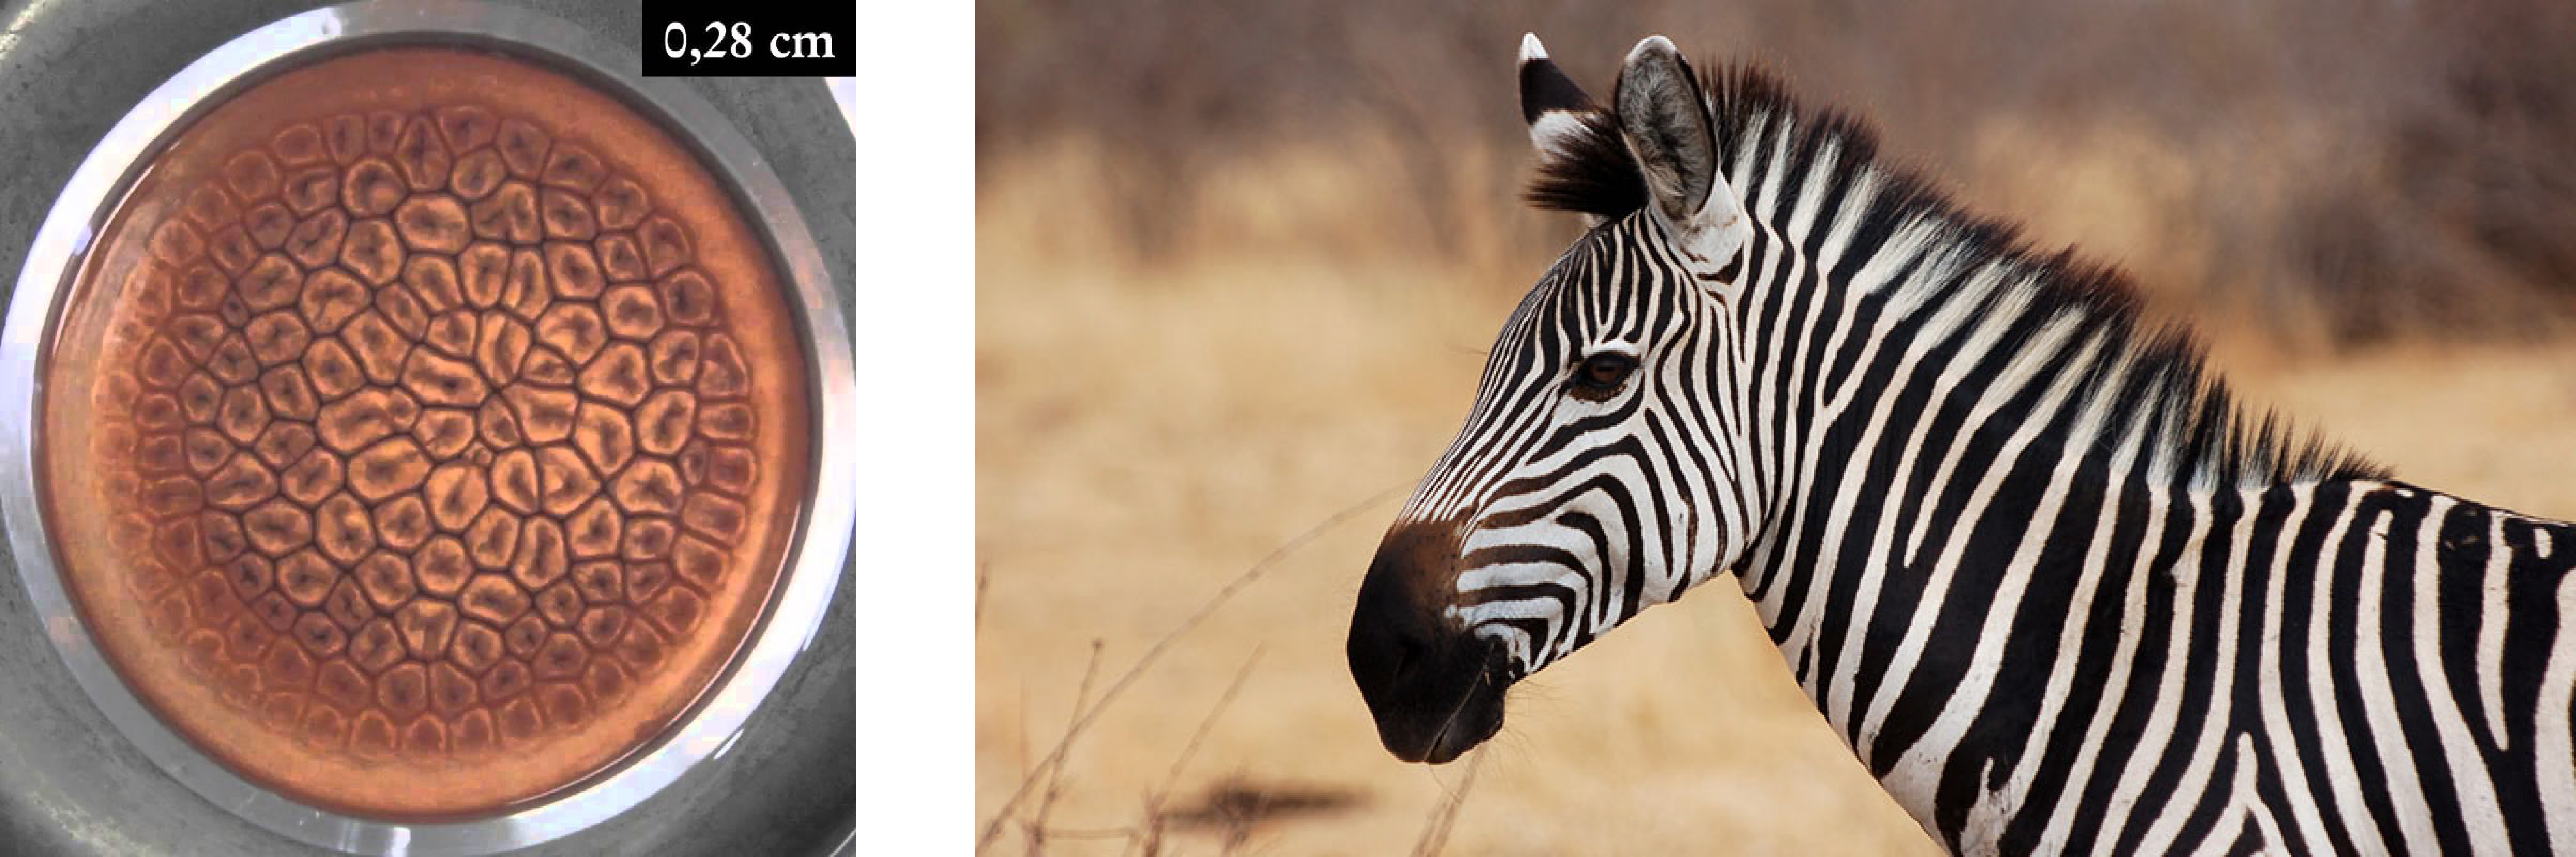
\includegraphics[width=14cm]{image/5-1-3.png}
\caption{自组织现象:\,B\'enard 对流与斑马身上的条纹}
\end{figure}


\npg{-10pt}

\section{理想气体}

\subsection{理想气体的定义}

满足以下三个条件的气体为理想气体:
\begin{enumerate}
	\item 分子间作用力可以忽略;
	\item 分子体积可以忽略;
	\item 分子按自由度平分能量.
\end{enumerate}

我们讨论一下这三个条件.\,首先第一个条件的意思,\,旨在把理想气体间的作用力当成\emph{短程力}(short-range force)处理.\,仅仅当两个分子间距离进入力程范围才可以当做可以发生相互作用(碰撞或散射).\,在这个意义下,\,分子体积实际上也可以处理为半径为力程大小的钢球模型.\,我们忽略这一个体积,\,也就是说所有分子可以自由活动的体积就等于容器体积$V$.\,且分子间相互作用力为零.

然而这两点合在一起将导致一个严重的问题:\,那便是热平衡不可以达到.\,若每个分子不可以通过相互作用或刚性的碰撞与别的分子交换能量与动量.\,那从根本上就不可以达到热平衡,\,统计方法也就无济于事.\,故分子体积足够小,\,小到可以忽略其对热力学性质的影响,\,但又足够大,\,大到在我们关心的时间空间尺度内体系能很快地达到热平衡.\,这才是对这两点的正确理解方式.

我们设分子的速率分布函数为$f(v)$,\,意思是每取$N$个分子,\,速率介于$v$到$v+\ud v$的分子数平均为:
\[\ud N=Nf(v)\ud v\]

从而分子的平均速率与方均速率为:
\[\overline{v}=\int_0^\infty vf(v)\ud v \quad ; \quad \overline{v^2}=\int_0^\infty v^2 f(v)\ud v\]

分子质量为$m$,\,直径为$D$,\,数密度为$n$.\,从中我们得出分子间平均距离$d$:
\[d\sim\frac{1}{\sqrt[3]{n}}\]

\begin{wrapfigure}[15]{o}[-10pt]{7cm}
\centering
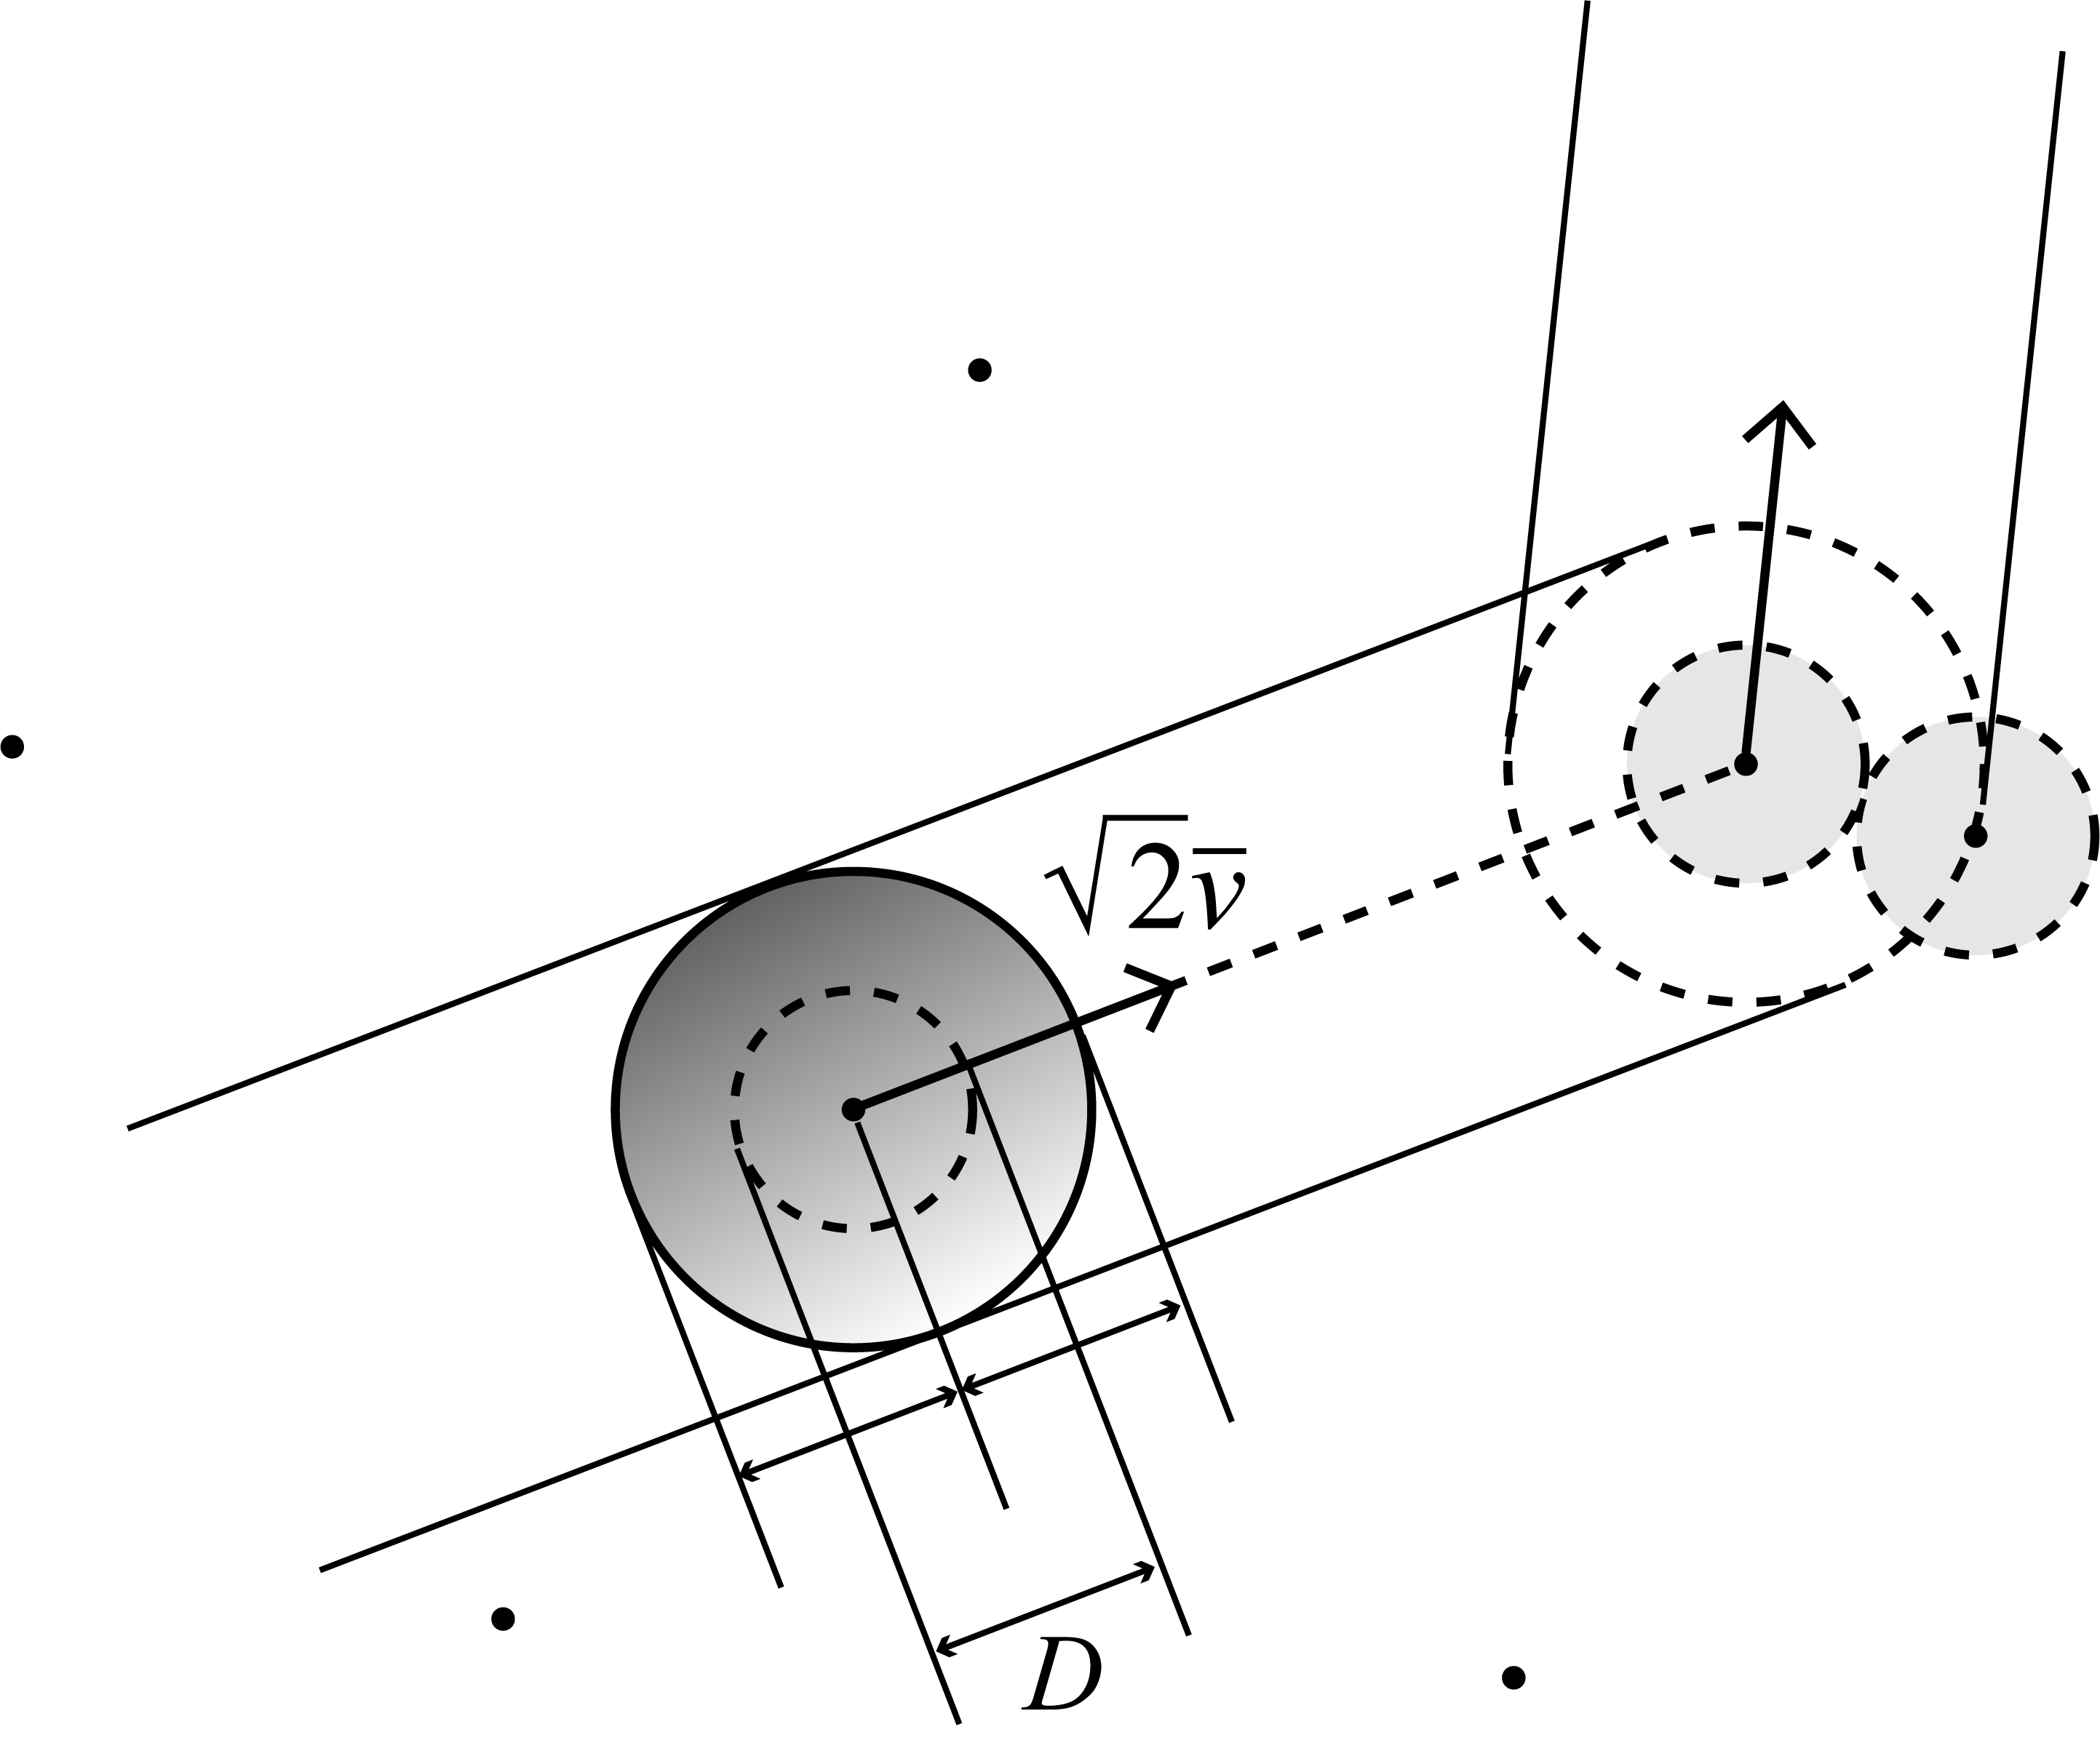
\includegraphics[width=6cm]{image/5-1-4.png}
\caption{曲折柱体计算}
\end{wrapfigure}
可以想见,\,分子间平均距离$d\sim 10{\rm nm}$(大气压下)越大,\,分子直径$D\sim 1{\rm nm}$越小,\,气体越能够近似为理想气体.\,同时其相隔两次碰撞的平均时间间隔$\tau$与空间间隔$\lambda$也会越大.\,如何计算这两个量呢?\,由于分子的速度符合麦克斯韦分布律(参见第五章),\,故两分子间的平均相对速率为$\sqrt{2}\overline{v}$.\,将待研究的粒子处理为钢球,\,速率恒定为$\sqrt{2}\overline{v}$,\,其半径为原分子直径$D$.而其他分子处理为静止的质点,\,半径为零.\,这样钢球碰到质点,\,即相当于原来的两个分子发生碰撞.\,而时间$t$内钢球扫过的体积为:
\[V(t)=\pi D^2\cdot \sqrt{2}\overline{v}t\]

发生碰撞次数$c$:
\[c(t)=nV(t)\]

当$c=1$时,\,对应的时间即为平均自由时间$\tau$,\,又称为\emph{驰豫时间}(relaxation time),\,而这一段时间内粒子走过的距离即为\emph{平均自由程}$\lambda$(mean free path):
\[\tau=\frac{1}{\sqrt{2}\pi nD^2\overline{v}} \quad ; \quad \lambda=\frac{1}{\sqrt{2}\pi nD^2}\]

即有:
\[\lambda\sim\frac{d^3}{D^2}\sim 100d\sim 1{\rm \upmu m}\]

以上数据仅仅在大气压下有效,\,注意平均自由程与分子平均速度无关,\,仅仅是一个几何相关量.\,而它与$n$成反比,\,也就是与$p$成反比,\,如果压强减小到约$1{\rm Pa}$(而温度不变),\,则平均自由程$\lambda$增大5个量级,\,也就是分米量级.

现在我们做一个总结:\,我们取了一个分子间相互作用力与分子的大小可以忽略的模型来研究理想气体,\,它对应的条件是:
\[D \ll d \quad ; \quad \lambda\sim\frac{d^3}{D^2} \ll L\]

第一个条件是保证分子体积可以忽略,\,第二个条件是在研究的问题尺度内保证分子有足够的空间来实现动量能量交换以达到热平衡.

现在让我们专心研究第三个条件.\,能量按自由度均分是麦克斯韦分布的一个独特结果.\,详情也可以参见第五章.\,现在我们指出,\,由于系统中的各个自由度,\,如$x,\,y,\,z$方向的平动,\,分子的转动,\,振动的能量具有相似的形式\footnote{指谐振子形式,\,详见第五章.},\,而且可以通过相互作用(碰撞)交换能量,\,总能量守恒.\,在这样的条件下,\,统计规律告诉我们每一个分子每一个自由度上都分得相同的平均能量值.\,这个平均能量值\footnote{及其对应的按能量高低的配分.}即代表了体系的温度:
\[\overline{\varepsilon}=\frac{1}{2}kT\]

体系自由度越多,\,分子数越多,\,在一定温度下储能就越多:
\[U=N\cdot\frac{f}{2}kT\]

其中$f$是系统能量自由度数\footnote{注意其与动力学自由度的区别,\,振动的势能也对应能量自由度,\,但其动力学自由度与振动动能重合.}.\,它被视为与温度无关的常量\footnote{然而实验发现这些不是常量,\,而是随着温度升高越来越大,\,存在一些基本不变的平台,\,思考这意味着什么.}.\,对于上式,\,我们再引入\emph{摩尔}(mole)这一化学计量单位来表示巨大的原子数$N$:
\[\frac{N}{N_A}=\nu \quad ; \quad N_A=6.022140857\pow{23}/{\rm mol}\]

同时,\,普适气体常量被定义为:
\[R=N_A k=8.314{\rm J/mol\cdot K}\]

这样气体的内能即为:
\[U=\frac{f}{2}\nu RT\]

\subsection{理想气体物态方程}
我们发现,\,$\ud p_1=f(v)\ud v$表示的含义为任意一个分子的速率落在$v\sim v+\ud v$区间内的概率.\,然而对于这样的分子,\,它速度方向在空间中的取向是任意的,\,各向同性的.\,所以建立极轴后,\,速度与极轴夹角在$\theta\sim\theta+\ud \theta$范围内的概率又为:
\[\ud p_2=\frac{\ud \Omega}{4\pi}=\frac{2\pi\sin\theta\ud\theta}{4\pi}=\frac{\sin\theta\ud\theta}{2}\]

对于这样的分子,\,它在容器中的任何位置都是有可能且等概率的,\,所以出现在体积微元$\ud V$中的概率还有$\ud p_3$,\,联合概率为$\ud p=\ud p_1\ud p_2\ud p_3$.

\begin{wrapfigure}[12]{o}[-10pt]{6cm}
\centering
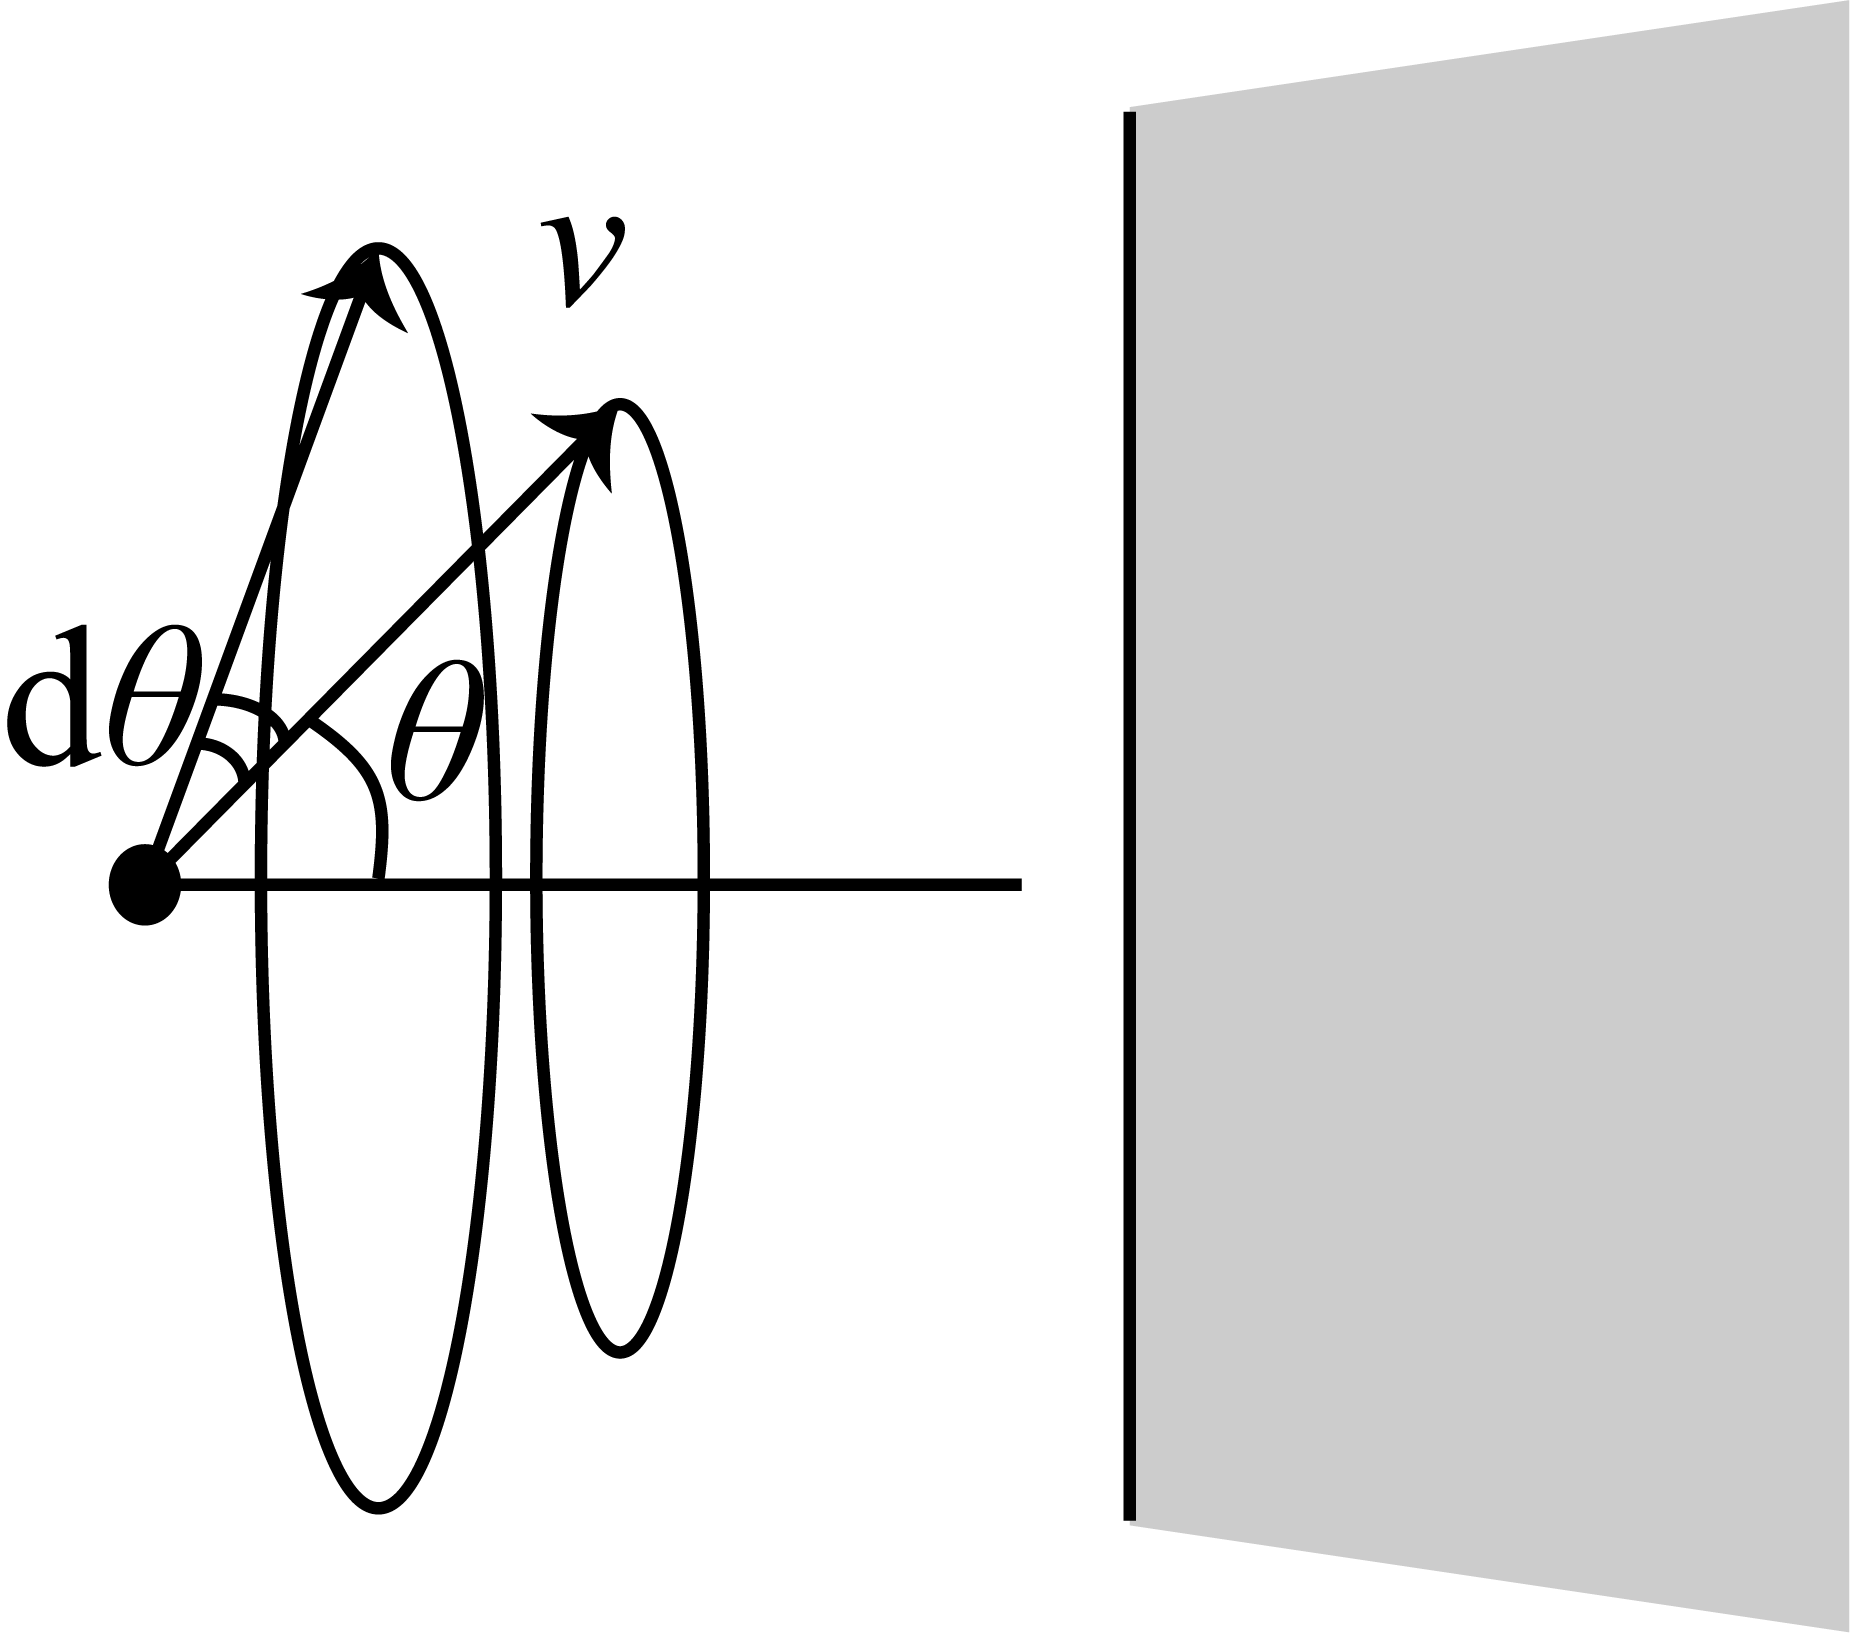
\includegraphics[width=6cm]{image/5-1-5.png}
\caption{粒子速度方向分布}
\end{wrapfigure}
我们接下来考虑气体的压强.\,在这之前我们了解两个概念是十分有帮助的:\,处于平衡态的系统可以看成互相达到平衡的各部分\emph{子系统}(subsystem)直接组成.\,这些部分的所有\emph{强度量}(intensive property)都是完全一致的,\,如理想气体的压强,\,温度,\,粒子数密度,\,摩尔体积,\,摩尔内能等等.\,而子系统的\emph{广延量}(extensive property)大小之和即为总系统的对应量的大小,\,如分子数,\,摩尔数,\,体积,\,内能,\,焓等等.\,我们可以这么理解:\,强度量描述体系的内禀属性,\,而广延量仅仅反应全同子系统的简单堆积.\,如一杯盐水,\,确定了我们关心的强度量\ca 温度和浓度之后,\,我们就可以回答``怎样的盐水''这一个问题.\,而接下来只需要再回答``有多少''这一个简单的问题,\,就能算出所有的广延量来.\,基于这一点理解,\,我们可以发现以下两个性质是成立的:\\[1pt]

{\hei 保持所有强度量不变,\,一个广延量变化$\lambda$倍,\,所有广延量随之变化$\lambda$倍.}\\[1pt]

{\hei 两个广延量之比为强度量,\,典型的如质量$M$比体积$V$为密度$\rho$,\,体积$V$比摩尔数$\nu$为摩尔体积$v$等.}\\[1pt]

理想气体作为极其简单的系统,\,它的独立强度量仅仅只有两个.\,一是系统的温度$T$.\,它决定了分子的平均热运动剧烈程度,\,也就是平均能量大小.\,另一个就是分子数密度$n$,\,它反映单位体积里有多少个全同单元,\,是一种``浓度''.\,其他所有强度量都是这两个量的导出.\,比如压强$p$,\,用分子动理论的方法:
\begin{eqnarray*}
p 	&=&	\int_0^{\infty}\int_0^{\frac{\pi}{2}}n\ud S v\cos\theta\ud t \cdot f(v)\ud v \cdot\frac{\sin\theta\ud\theta}{2}\cdot 2mv\cos\theta/\ud S\ud t 	\\
	&=&	nm\cdot\int_0^{\infty}v^2 f(v)\ud v \cdot \int_0^{\frac{\pi}{2}}\sin\theta\cos^2\theta\ud\theta	\\
	&=& \frac{1}{3}nm\overline{v^2}		\\
	&=& \frac{2}{3}n\overline{\varepsilon_k}	\\
	&=& nkT
\end{eqnarray*}

可见对容器壁的压强正比于温度和分子数密度,\,这一点的物理图像还是很直观的.\,这个压强被我们称之为\emph{外压强}(outer pressure).\,它是由于分子碰撞容器壁引起.\,还有所谓的\emph{内压强}(inner pressure)的概念,\,它由于分子间的碰撞引起.\,理想气体的内压强与外压强相等\footnote{然而范德瓦尔斯气体则不然,\,详见第四章.}.\,但如果气体足够稀薄,\,以至于容器尺度与分子平均自由程可以比拟.\,此时内压强的概念也失去了意义,\,这意味着气体完全不可以用动力学方法处理,\,压强的梯度不会导致气体团的加速度,\,而是以下面所介绍的泻流的方式进行.

上文我们推出来的关系式被称作(强度量之间的)\emph{物态方程}(equation of state),\,它有很多变式,\,如:
\[pV=NkT \quad ; \quad pV=\nu RT \quad ; \quad pv=RT \quad ; \quad p=\frac{\rho RT}{\mu}\]

上面最后一式中$\mu$表示摩尔质量,\,稍作变形还可以得到密度公式:
\[\rho=\frac{\mu p}{RT}\]

用分子动理论方法还可以得到另一个十分重要的量\ca \emph{泻流数}(effusion number).\,如果在容器壁上开一个小孔.\,则速率在在$v$到$v+\ud v$区间内的分子,\,单位面积单位时间通过小孔的分子数为:
\begin{eqnarray*}
\ud \Gamma 		&=& 	\int_0^{\frac{\pi}{2}}n\ud S v\cos\theta\ud t \cdot f(v)\ud v \cdot\frac{\sin\theta\ud\theta}{2}/\ud S\ud t 	\\
				&=&		\frac{n}{2}\cdot \int_0^{\frac{\pi}{2}}\sin\theta\cos\theta\ud\theta	\\
				&=&		\frac{1}{4} nv f(v)\ud v 	\\
				&=&		\frac{1}{4}\ud n v
\end{eqnarray*}
可见速率为$v$的那一部分分子,\,泻流数就是$\ud \Gamma=\frac{1}{4} \ud nv$.\,那么对于所有分子,\,总泻流数为:
\[\Gamma=\frac{1}{4}n\overline{v}\]

泻流的条件是开的孔的大小足够小,\,以至于分子在穿过孔时不会受到别的分子的碰撞.\,也就是其平均自由程$\lambda$显著地大于孔的直径$L$.\,相反地,\,如果$\lambda\ll L$,\,那么就变成了一种压强差驱动气体集团运动的动力学模型,\,我们在下一节阐述.

最后,\,理想气体的内能则可以根据之前关于温度定义的讨论,\,直接写出:
\[U=\nu C_{mV} T\]

其中$C_{mV}$被称为\emph{定容摩尔热容}(molar heat capacity at constant volume).\,其意义之后将了解.\,现在只需知道$\displaystyle C_{mV}=\frac{f}{2}R$.

\subsection{混合理想气体}
考虑几种理想气体的混合,\,我们也需要忽略几种组分分子间的相互作用,\,尤其是应该排除几种分子间发生化学反应的情况\footnote{如混合{$\rm NH_3$}与{$\rm Cl_2$}.}.\,此时,\,几种气体由各自的数密度$n_i$和热平衡下的公共温度$T$描述.\,另一种描述方法是给出总分子数密度$n$与各组分分子所占的比例(强度量)$x_i$:
\[n=\sum n_i \quad ; \quad x_i=\frac{n_i}{n}\]

称为\emph{摩尔分数}(mole fraction),\,注意$x_i$间要满足的归一关系:
\[\sum x_i=1\]

不同组分间分子纵然有碰撞,\,但这对于这一部分分子碰撞容器壁产生的压强大小没有影响.\,也就是说,\,压强等于各组分以$n_i$单独存在时对容器壁产生的分压$p_i$.\,这叫做\emph{道尔顿分压定律}({\it Dalton}'s law of partial pressures):
\[p=\sum p_i \quad ;\quad p_i=n_i kT=x_i p \quad ; \quad p=nkT\]

值得注意,\,每个分子的质量$m_i$或能量自由度数$i_i$并不影响压强的计算.\,压强单方面地决定于分子数密度与温度(分子平均平动动能.\,分子质量改变的是整个体系的摩尔质量$\mu$,\,取一定体积的气体:
\[M=\nu\mu=\sum M_i=\sum \nu_i\mu_i \quad \Rightarrow \quad \mu=\sum x_i \mu_i\]

其中出现的摩尔数$\nu_i$之比即为分子数密度$n_i$之比,\,而摩尔质量$\mu_i$与分子质量的换算关系也很基础,\,请读者一定要熟练使用:
\[\nu_i : \nu_j=\frac{n_i V}{N_A} : \frac{n_j V}{N_A}=n_i : n_j \quad ; \quad \mu_i=N_A m_i\]

能量自由度数影响的是摩尔内能$u$:
\[u=\nu \overline{C_{mV}} T=\sum u_i=\sum \nu_i C_{mVi} T \quad \Rightarrow \quad \overline{C_{mV}}=\sum x_i C_{mVi}=\sum \frac{x_i f_i}{2}R\]

上面我们定义了平均摩尔定容热容$\overline{C_{mV}}$.\,平均的含义一定是按分子数$n_i$(摩尔数$\nu_i$,\,比例$x_i$)平均.

\subsection{理想气体的过程}
\begin{wrapfigure}[15]{o}[-10pt]{6cm}
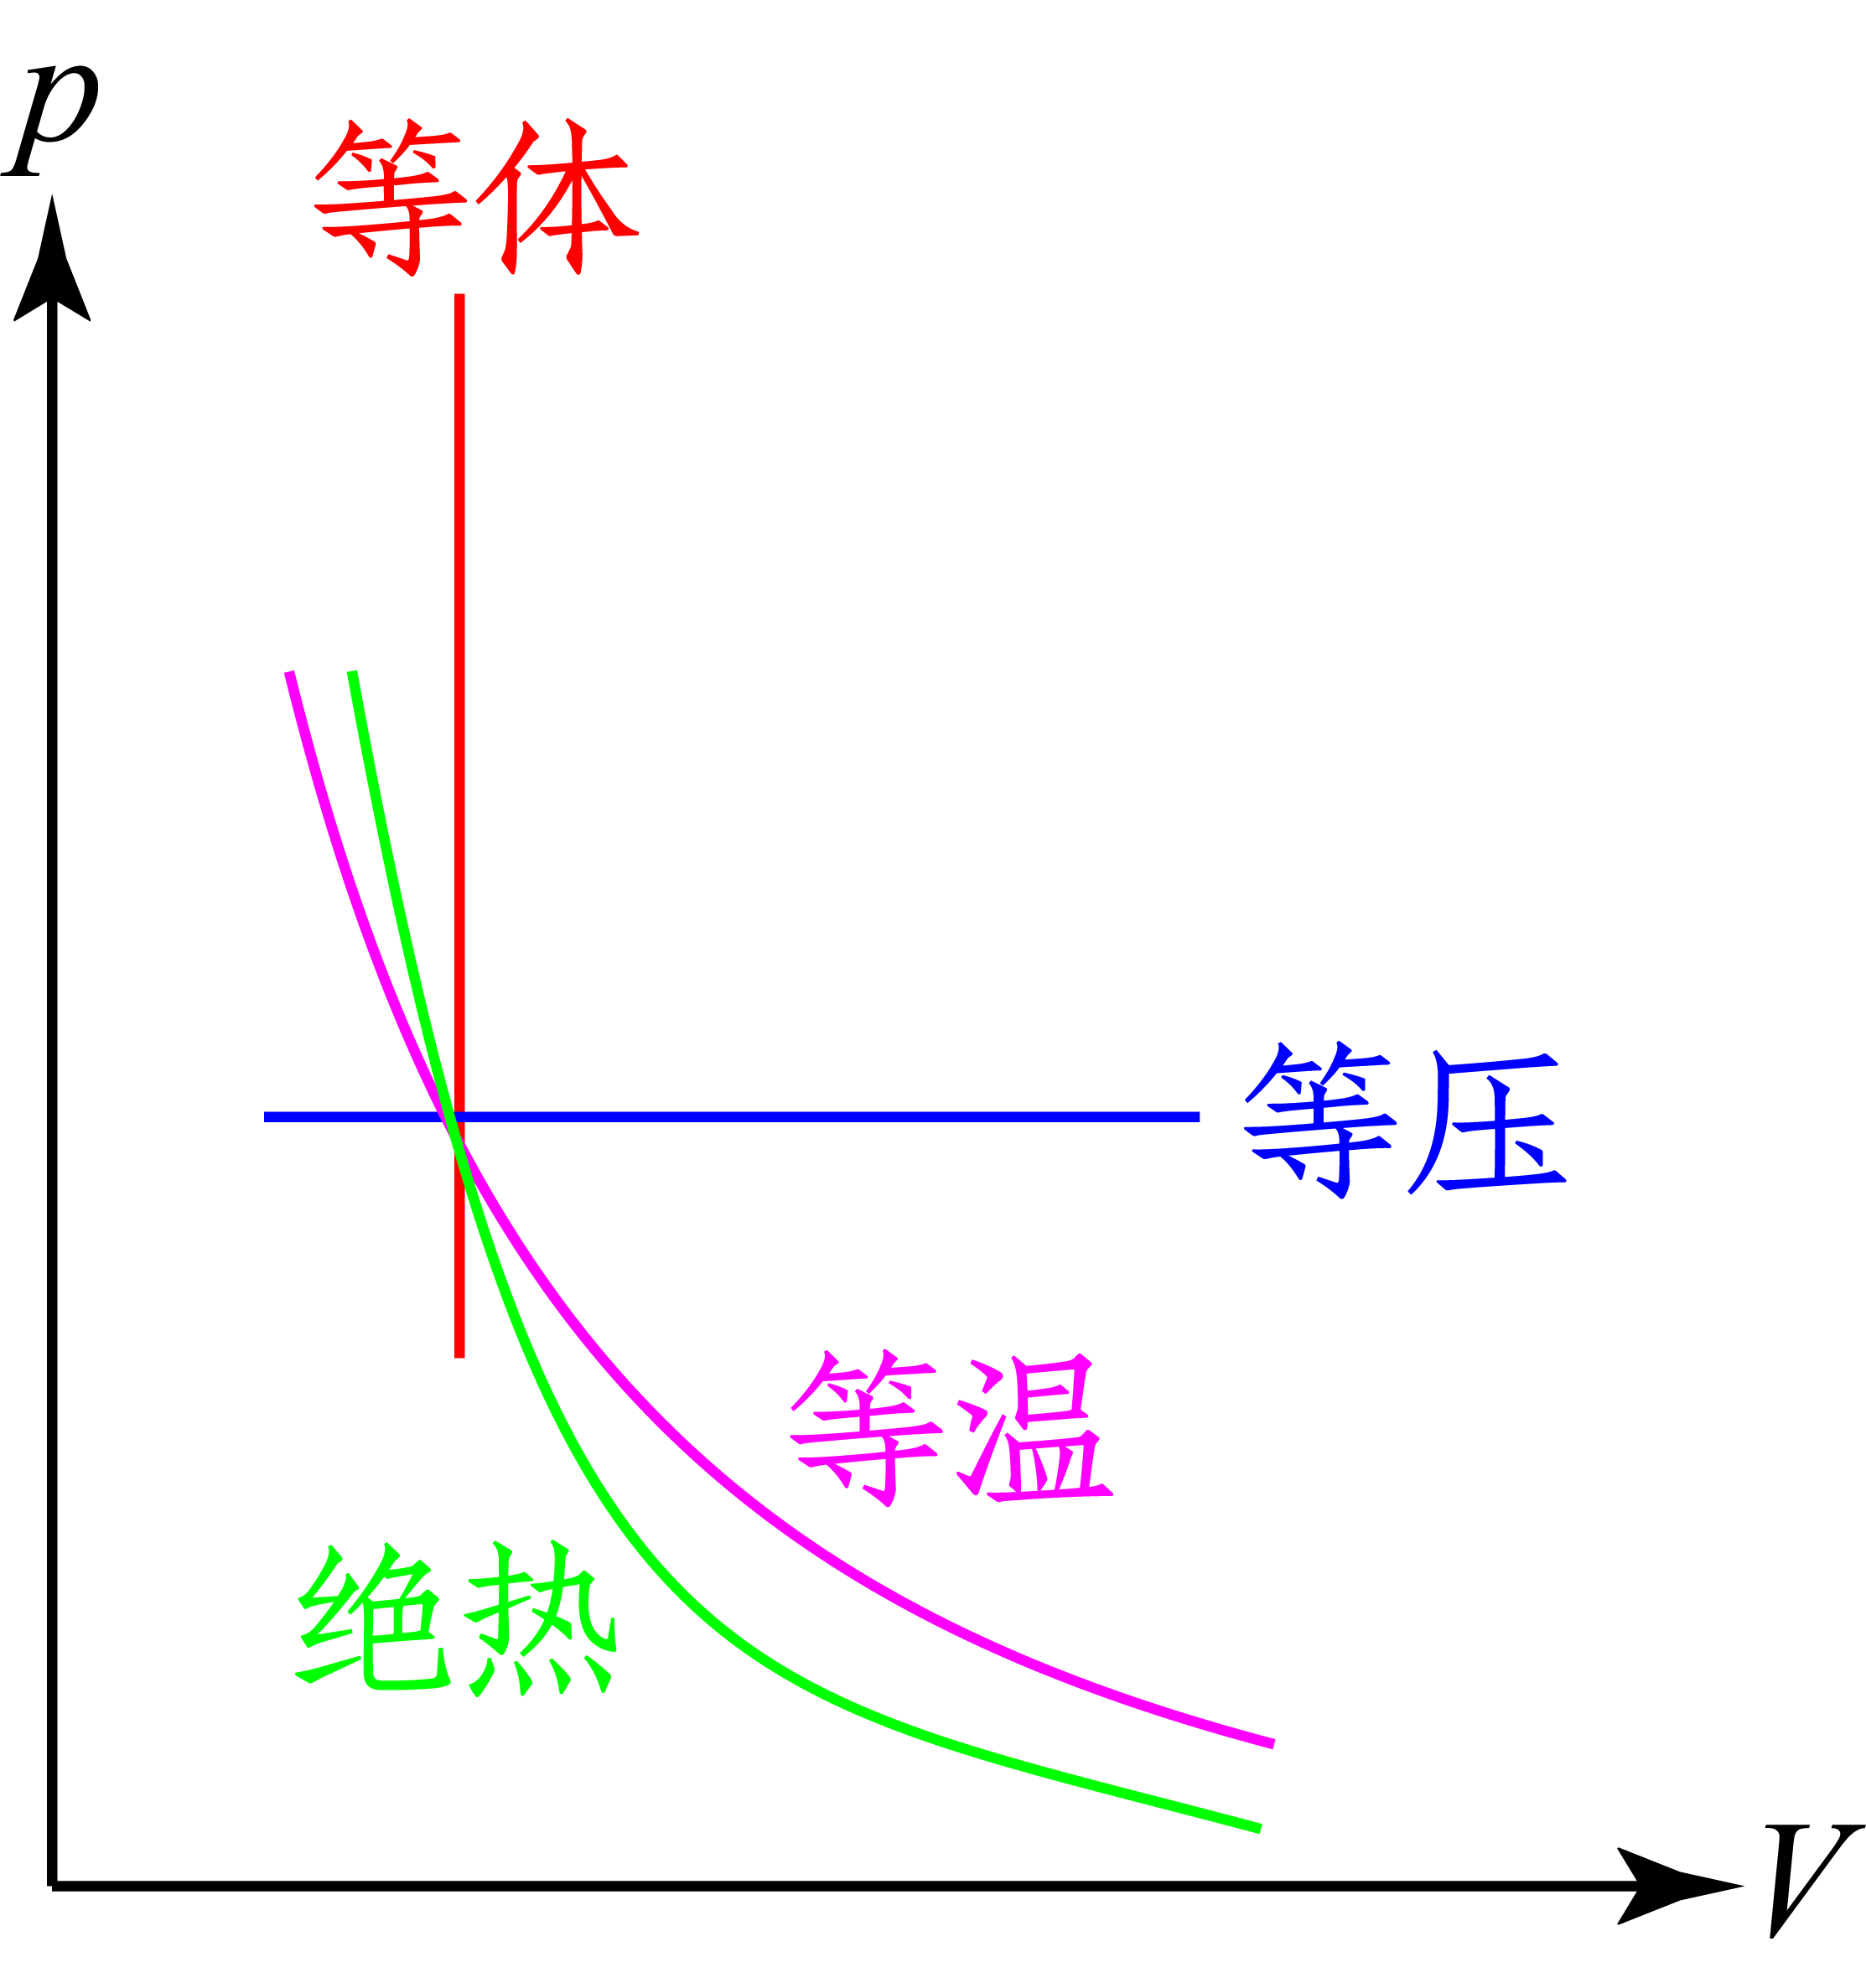
\includegraphics[width=6cm]{image/5-1-6.png}
\caption{四大准静态过程}\label{fig:1-6}
\end{wrapfigure}
所谓\emph{过程}(process)是状态的集合.\,我们考虑的范围内,\,过程的初态和末态都需要是均匀的平衡态.\,中间态如果也可以视为平衡态,\,就叫做\emph{准静态过程}(quasi-static process),\,若中间态蕴含着非平衡,\,则称为\emph{非准静态过程}(non-quasi-static process).\,下面列举常见的过程:
\subsubsection{\hei 等体过程(isochoric process)}
作为等体过程体积功为零$W=0$,\,只能以从外界吸放热$Q$(或是如图\ref{fig:1-2}所示的功变热形式.).\,系统吸热导致温度$T$升高,\,定义系统\emph{热容}(heat capacity)为:
\[C=\frac{\dbar Q}{\ud T}\]

而压强$p$将升高,\,定义\emph{压强系数}(pressure coefficient)为:
\[\beta:=\frac{1}{p}\frac{\ud p}{\ud T}\]

根据理想气体的物态方程与内能公式我们算出\footnote{热力学的角标表示这个量不变,\,而这里热容的表达式下一章学了熵的概念后可以写:\[C=T\frac{\partial S}{\partial T}\]}:
\[C_V=\left(\frac{\dbar Q}{\ud T}\right)_V=\nu C_{mV} \quad ; \quad \beta_V=\frac{1}{p}\left(\frac{\partial p}{\partial T}\right)_V=\frac{1}{T}\]

\subsubsection{\hei 准静态的等压过程(isobaric process)}
若是控制压强$p$而不是体积$V$不变,\,区别在于气体从外界吸收的热量中一部分要用来对外做功:
\[\ud U=\dbar Q-p\ud V\]

热容按同样的方法定义,\,分别称为等体热容和等压热容\footnote{中文太灵活,\,``等体''也有人说成``定体'',\,``等容'',\,``定容''.\,统一术语十分困难.}.\,而\emph{热膨胀系数}(thermal expansion coefficient)定义为:
\[\alpha:=\frac{1}{V}\frac{\ud V}{\ud T}\]

注意这实际上是\emph{体膨胀系数}(volumetric thermal expansion),\,由近似方法可知,\,近似为线膨胀系数$\alpha_L$的三倍.\,对于理想气体等压过程,\,同理可得:
\[C_p=\left(\frac{\dbar Q}{\ud T}\right)_p=\nu (C_{mV}+R)=\nu C_{mp} \quad ; \quad \alpha=\frac{1}{V}\left(\frac{\partial V}{\partial T}\right)_p=\frac{1}{T}\]

\subsubsection{\hei 准静态的等温过程(isothermal process)}
系统与恒温大热库接触,\,吸热膨胀, 压强减小;\,放热收缩,\,压强增大.\,这时$pV$为过程不变量.\,我们定义\emph{压缩系数}(compression coefficient):
\[\kappa:=-\frac{1}{V}\frac{\ud V}{\ud p}\]

注意若是在固体情形,\,以上量被称为\emph{体模量}(bulk modulus).\,对于理想气体,\,等温压缩系数为:
\[\kappa_T=-\frac{1}{V}\left(\frac{\partial V}{\partial p}\right)_T=\frac{1}{p}\]

\subsubsection{\hei 准静态的绝热过程(adiabatic process)}
绝热过程中$\dbar Q=0$,\,对于理想气体:
\[\ud U +p \ud V=0\]
\[\nu C_{mV} \ud T + \frac{\nu R T}{V}\ud V=0\]
\[C_{mV}\frac{\ud T}{T}+R\frac{\ud V}{V}=0\]

惯例上定义\emph{绝热指数}(adiabatic index)$\gamma$为:
\[\gamma:=\frac{C_{mp}}{C_{mV}}=1+\frac{R}{C_{mV}}=\frac{f+2}{f}\]

则可以由$\gamma$和$R$表示两个摩尔热容:
\[C_{mV}=\frac{1}{\gamma -1}R \quad ;\quad C_{mp}=\frac{\gamma}{\gamma -1}R\]

从而我们从绝热过程的热力学第一定律方程积分得:
\[TV^{\gamma-1}={\rm Const.}\]

也可以写为:
\[pV^\gamma={\rm Const.} \quad ; \quad \frac{p^{\gamma-1}}{T^\gamma}={\rm Const.}\]

前一式可以用于在$p-V$图\ref{fig:1-6}上确定过程曲线.\,后一式则注重关心强度量之间的变化关系而不关心广延性质.\,在绝热过程中(用角标$S$表示绝热,\,$S$其实表示熵,\,具体原因见下一章.),\,热膨胀系数,\,压强系数与压缩系数分别为:
\[\alpha_S=\frac{1}{V}\left(\frac{\partial V}{\partial T}\right)_S=-\frac{1}{\gamma -1}\frac{1}{T} \quad ;\quad \beta_S=\frac{1}{p}\left(\frac{\partial p}{\partial T}\right)_S=\frac{\gamma}{\gamma -1}\frac{1}{T}\quad ;\quad \kappa_S=-\frac{1}{V}\left(\frac{\partial V}{\partial p}\right)_S=\frac{1}{\gamma}\frac{1}{p}\]

\subsubsection{\hei 准静态的多方过程(polytropic process)}
多方过程可以由过程方程$pV^n={\rm Const.}$描述,\,多方指数$1<n<\gamma$.\,实际过程若发生缓慢,\,可以近似处理为某种形式的多段多方过程.\,多方过程的热容为:
\[C_{mn}=\left(\frac{1}{\gamma -1}-\frac{1}{n-1}\right)R\]

而其他响应函数(指上面定义的$\alpha$,\,$\beta$与$\kappa$)的形式与绝热过程算出来的类似,\,只需要把$\gamma$改为$n$.\,多方过程在特殊的参数条件下即变成以上过程:
\begin{figure}[H]
\centering
\begin{tabular}{c|c|l}
\hline
绝热指数$n$		&	摩尔热容$C_m$						&	描述			\\ \hline\hline
$n<0$ 			   		&	$\left(\dfrac{1}{\gamma -1}+\dfrac{1}{1-n}\right)R$ 		&	 吸收大量热量,\,压强体积温度同时增加			\\ \hline
$n=0$				  &	$C_{mp}$    																				&   等压过程 		    \\ \hline
$0<n<1$			&   $\left(\dfrac{1}{\gamma -1}+\dfrac{1}{1-n}\right)R$ 				&   相比吸热等温膨胀,\,温度有升高				\\ \hline
$n=1$		&	$\infty$ 																									&  	等温过程 			\\ \hline
$1<n<\gamma$		&	$ -\left(\dfrac{1}{n -1}-\dfrac{1}{\gamma -1}\right)R$ 				& 	膨胀降温时要从外界吸热 			\\ \hline
$n=\gamma$		&	$0$ 																									&	绝热过程 			\\ \hline
$n>\gamma$		&	$\left(\dfrac{1}{\gamma -1}-\dfrac{1}{n-1}\right)R$						& 	压缩气体同时给气体热量的过程	\\ \hline
$n=\infty$		&	$C_{mV}$ 																						&	等温过程			\\ \hline
\end{tabular}
\end{figure}

\subsubsection{\hei 自由膨胀过程}
\begin{wrapfigure}[15]{o}[-10pt]{6cm}
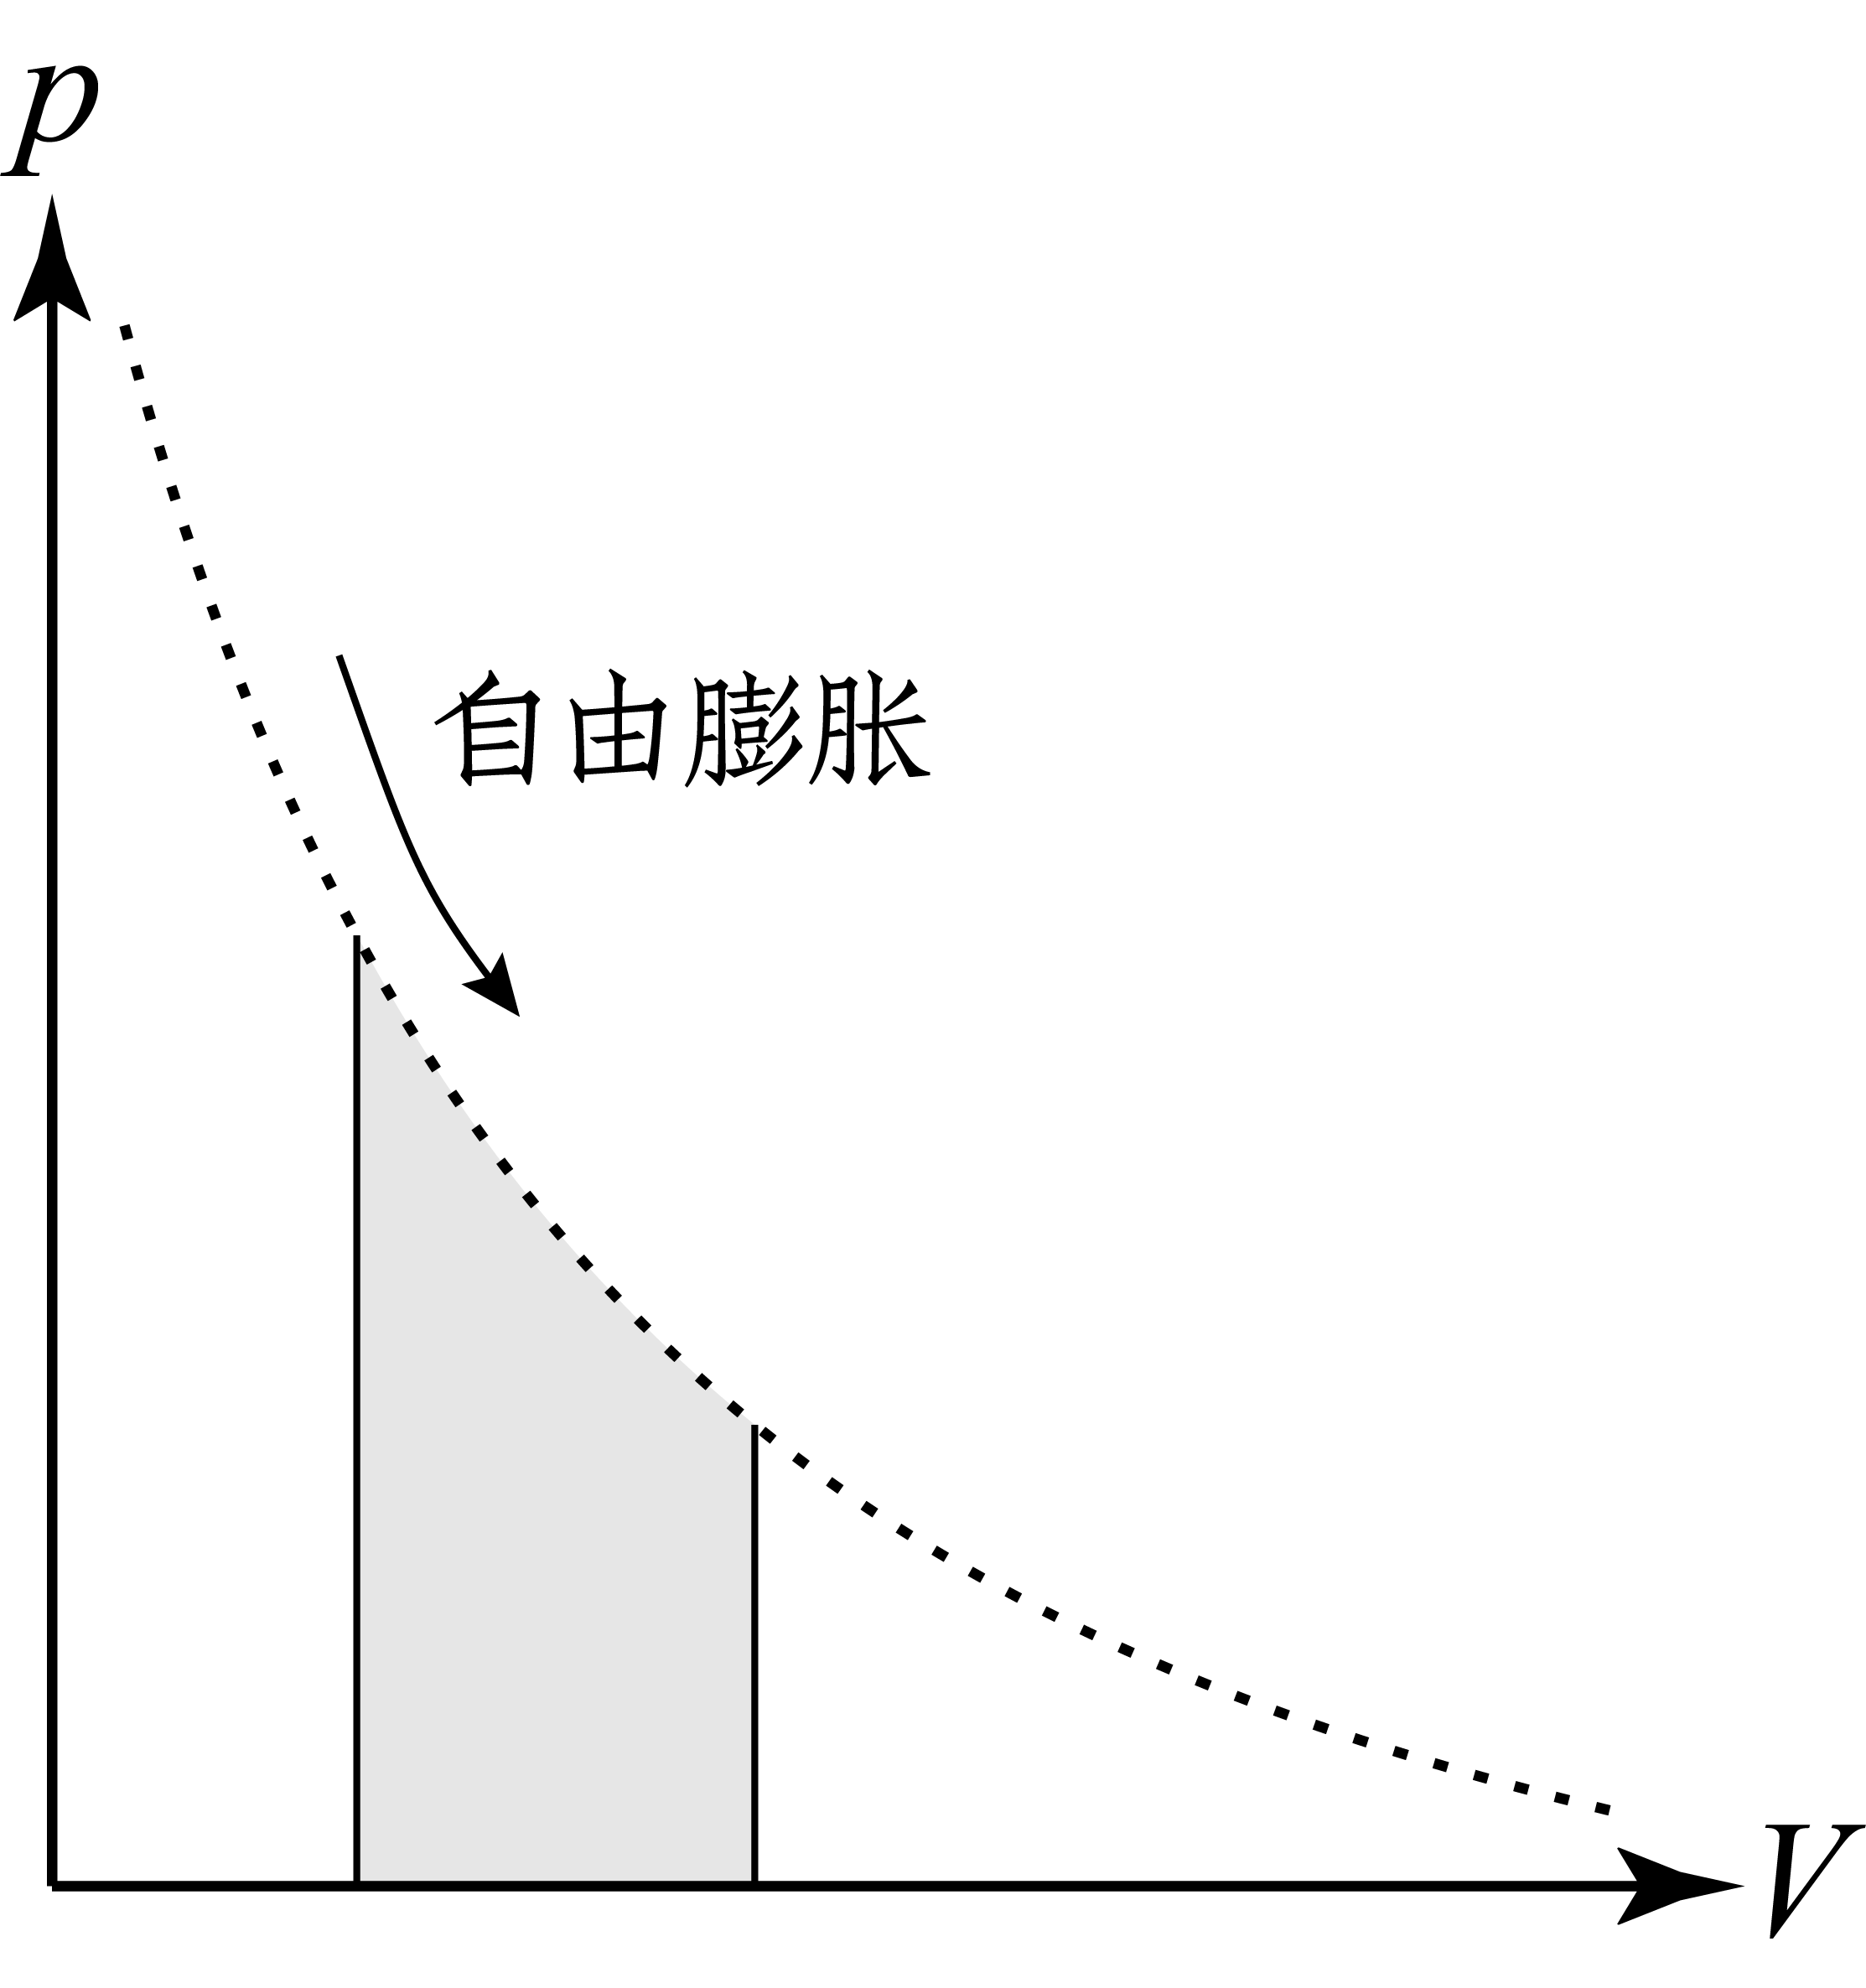
\includegraphics[width=6cm]{image/5-1-7.png}
\caption{$p-V$图上画自由膨胀}
\end{wrapfigure}
理想气体向真空的\emph{自由膨胀过程}(free expansion process)是一类典型的非准静态过程.\,在这样一个过程中,\,由于外压为零,\,外界对气体做功为零.\,而系统绝热,\,从而从外界吸热也为零.\,故由于热力学第一定律,\,内能不变.\,再根据理想气体内能直接依赖于温度的性质,\,我们发现:\,理想气体的自有膨胀是一个非准静态的等温膨胀.

从而在$p-V$图上,\,我们画一根等温线,\,它是否代表向真空的自由膨胀过程?\,我们需要画成虚线,\,线上每一个点都表示平衡态,\,而从一个点到另一个相邻的点中发生的过程则没有达到力学平衡,\,从而不能视为准静态过程.\,这一根虚线能够代表气体在自有膨胀过程中的状态,\,因为即使不均匀,\,整体的内能和可以确定出平均温度,\,整体的体积和平均温度又可以确定出平均压强.\,如果在某个时刻命自有膨胀结束,\,体系达到平衡态后其状态就落在了这根等温线上.\,只不过,\,这根线下面积此时也没有了实际意义,\,因为气体对外做功应该是零.

\vspace{2cm}

\subsubsection{\hei 向固定压强膨胀}
\begin{wrapfigure}[11]{o}[-10pt]{6cm}
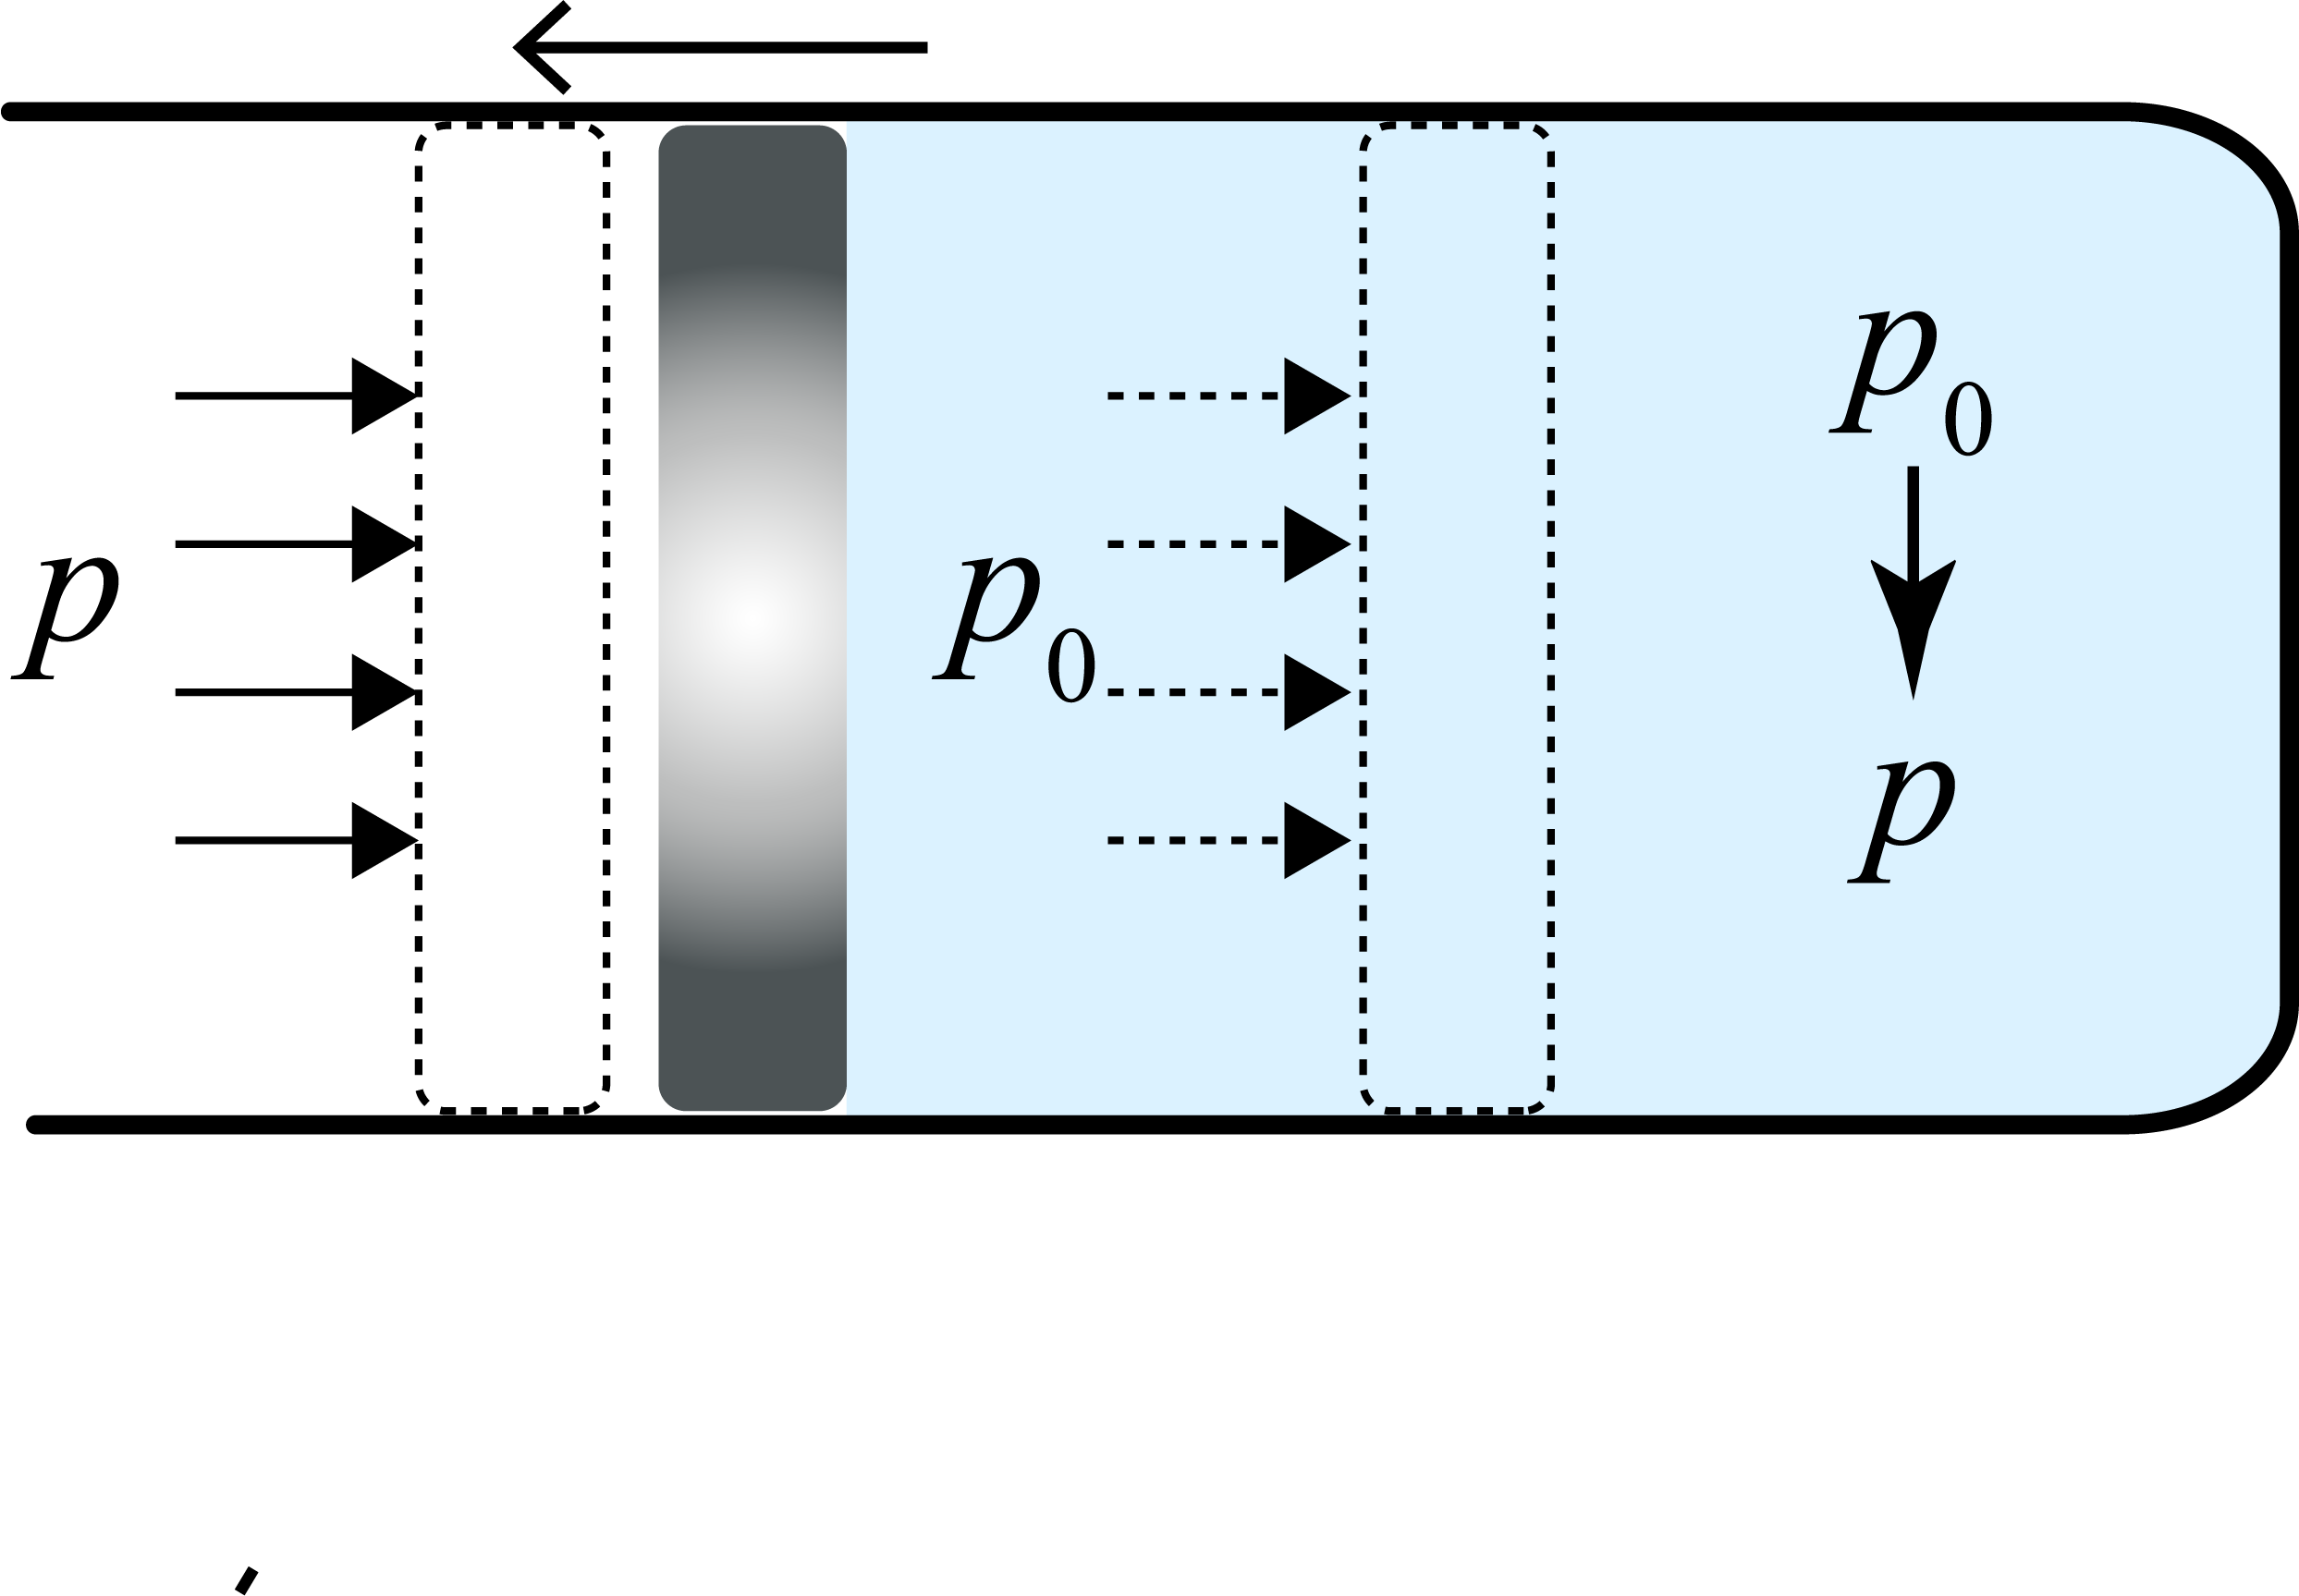
\includegraphics[width=6cm]{image/5-1-8.png}
\caption{向固定压强膨胀}
\end{wrapfigure}
考虑原平衡态压强为$p_0$的气体,\,突然命外压变小为$p$,\,气体将发生某种膨胀,\,如果膨胀稍过度,\,其压强小于外界压强$p$时,\,又会被压缩,\,这样来回振动,\,直到达到新的平衡态.\,如果这个过程系统绝热,\,则系统对外界做功应该写为:
\[W=p(V-V_0)\]

这一个模型可以这样理解:\,它保证了外界压强$p$的严格不变性.\,内部气体由于发生了急剧的体积变化,\,最靠近活塞的部分气体压强由于急剧的膨胀实际上就会等于外界气压$p$.\,这是忽略活塞质量(轻活塞)的情形.\,若是考虑活塞的质量,\,这个结论也还是成立,\,因为内外气体对活塞做功之和转化为活塞动能.\,而前后平衡态活塞实际上动能都是零.\,故内部气体对外做功可以由外界固定压强部分气体的体积功来计算.\,这就是上式.\,那么同样,\,由热力学第一定律和理想气体的性质,\,我们有:
\[\frac{V}{V_0}=1+\frac{p_0-p}{\gamma p} \quad ; \quad \frac{T}{T_0}=\frac{1}{\gamma}+(1-\frac{1}{\gamma})\frac{p}{p_0}\]

如果我们在初态压强$p_0$与末态压强$p$之间搭设很多的压强平台$p_i$,\,使得外压是缓慢地从$p_0$逐级减小到$p$,\,那么用极限的方法容易证明(请读者自己完成),\,过程恰好变为准静态的绝热过程:
\[pV^\gamma=p_0V_0^\gamma \quad ; \quad \frac{p^{\gamma-1}}{T^\gamma}=\frac{p_0^{\gamma-1}}{T_0^\gamma}\]

此时屡次的非平衡态将无限趋于平衡态,\,而非准静态过程也就无限趋于准静态过程了.

\npg{-2cm}

\subsubsection{\hei 节流过程(throttling)}
节流过程亦是对很多复杂系统过程的抽象,\,如冷凝机内部工作物质所发生的循环的定常流动.\,我们从中提取出一个模型,\,如下图,\,气体在内壁光滑的管道内做定常流动,\,通过一多孔塞后压强减小,\,气体膨胀.\,整个过程绝热.\,我们取一个固定的气团(图中红加蓝)作为研究对象.\,经过一定时间$t$后左侧与右侧体积变化分别为$V_1$与$V_2$,\,那么气体的流量被定义为:
\[Q=\frac{m_i}{t}=\frac{\rho_i V_i}{t}=\rho_i v_i A\]

由于是定常流动,\,左右两侧流量必须相等,\,这是质量守恒的要求,\,而体积流量$v_i A$可以不相等,\,因为气体可以被压缩.

下面我们考虑气体的热力学第一定律,\,由于$Q$小,\,我们忽略气体的整体动能(这一点在下一节我们将做详细讨论).\,
\begin{figure}[H]
\centering
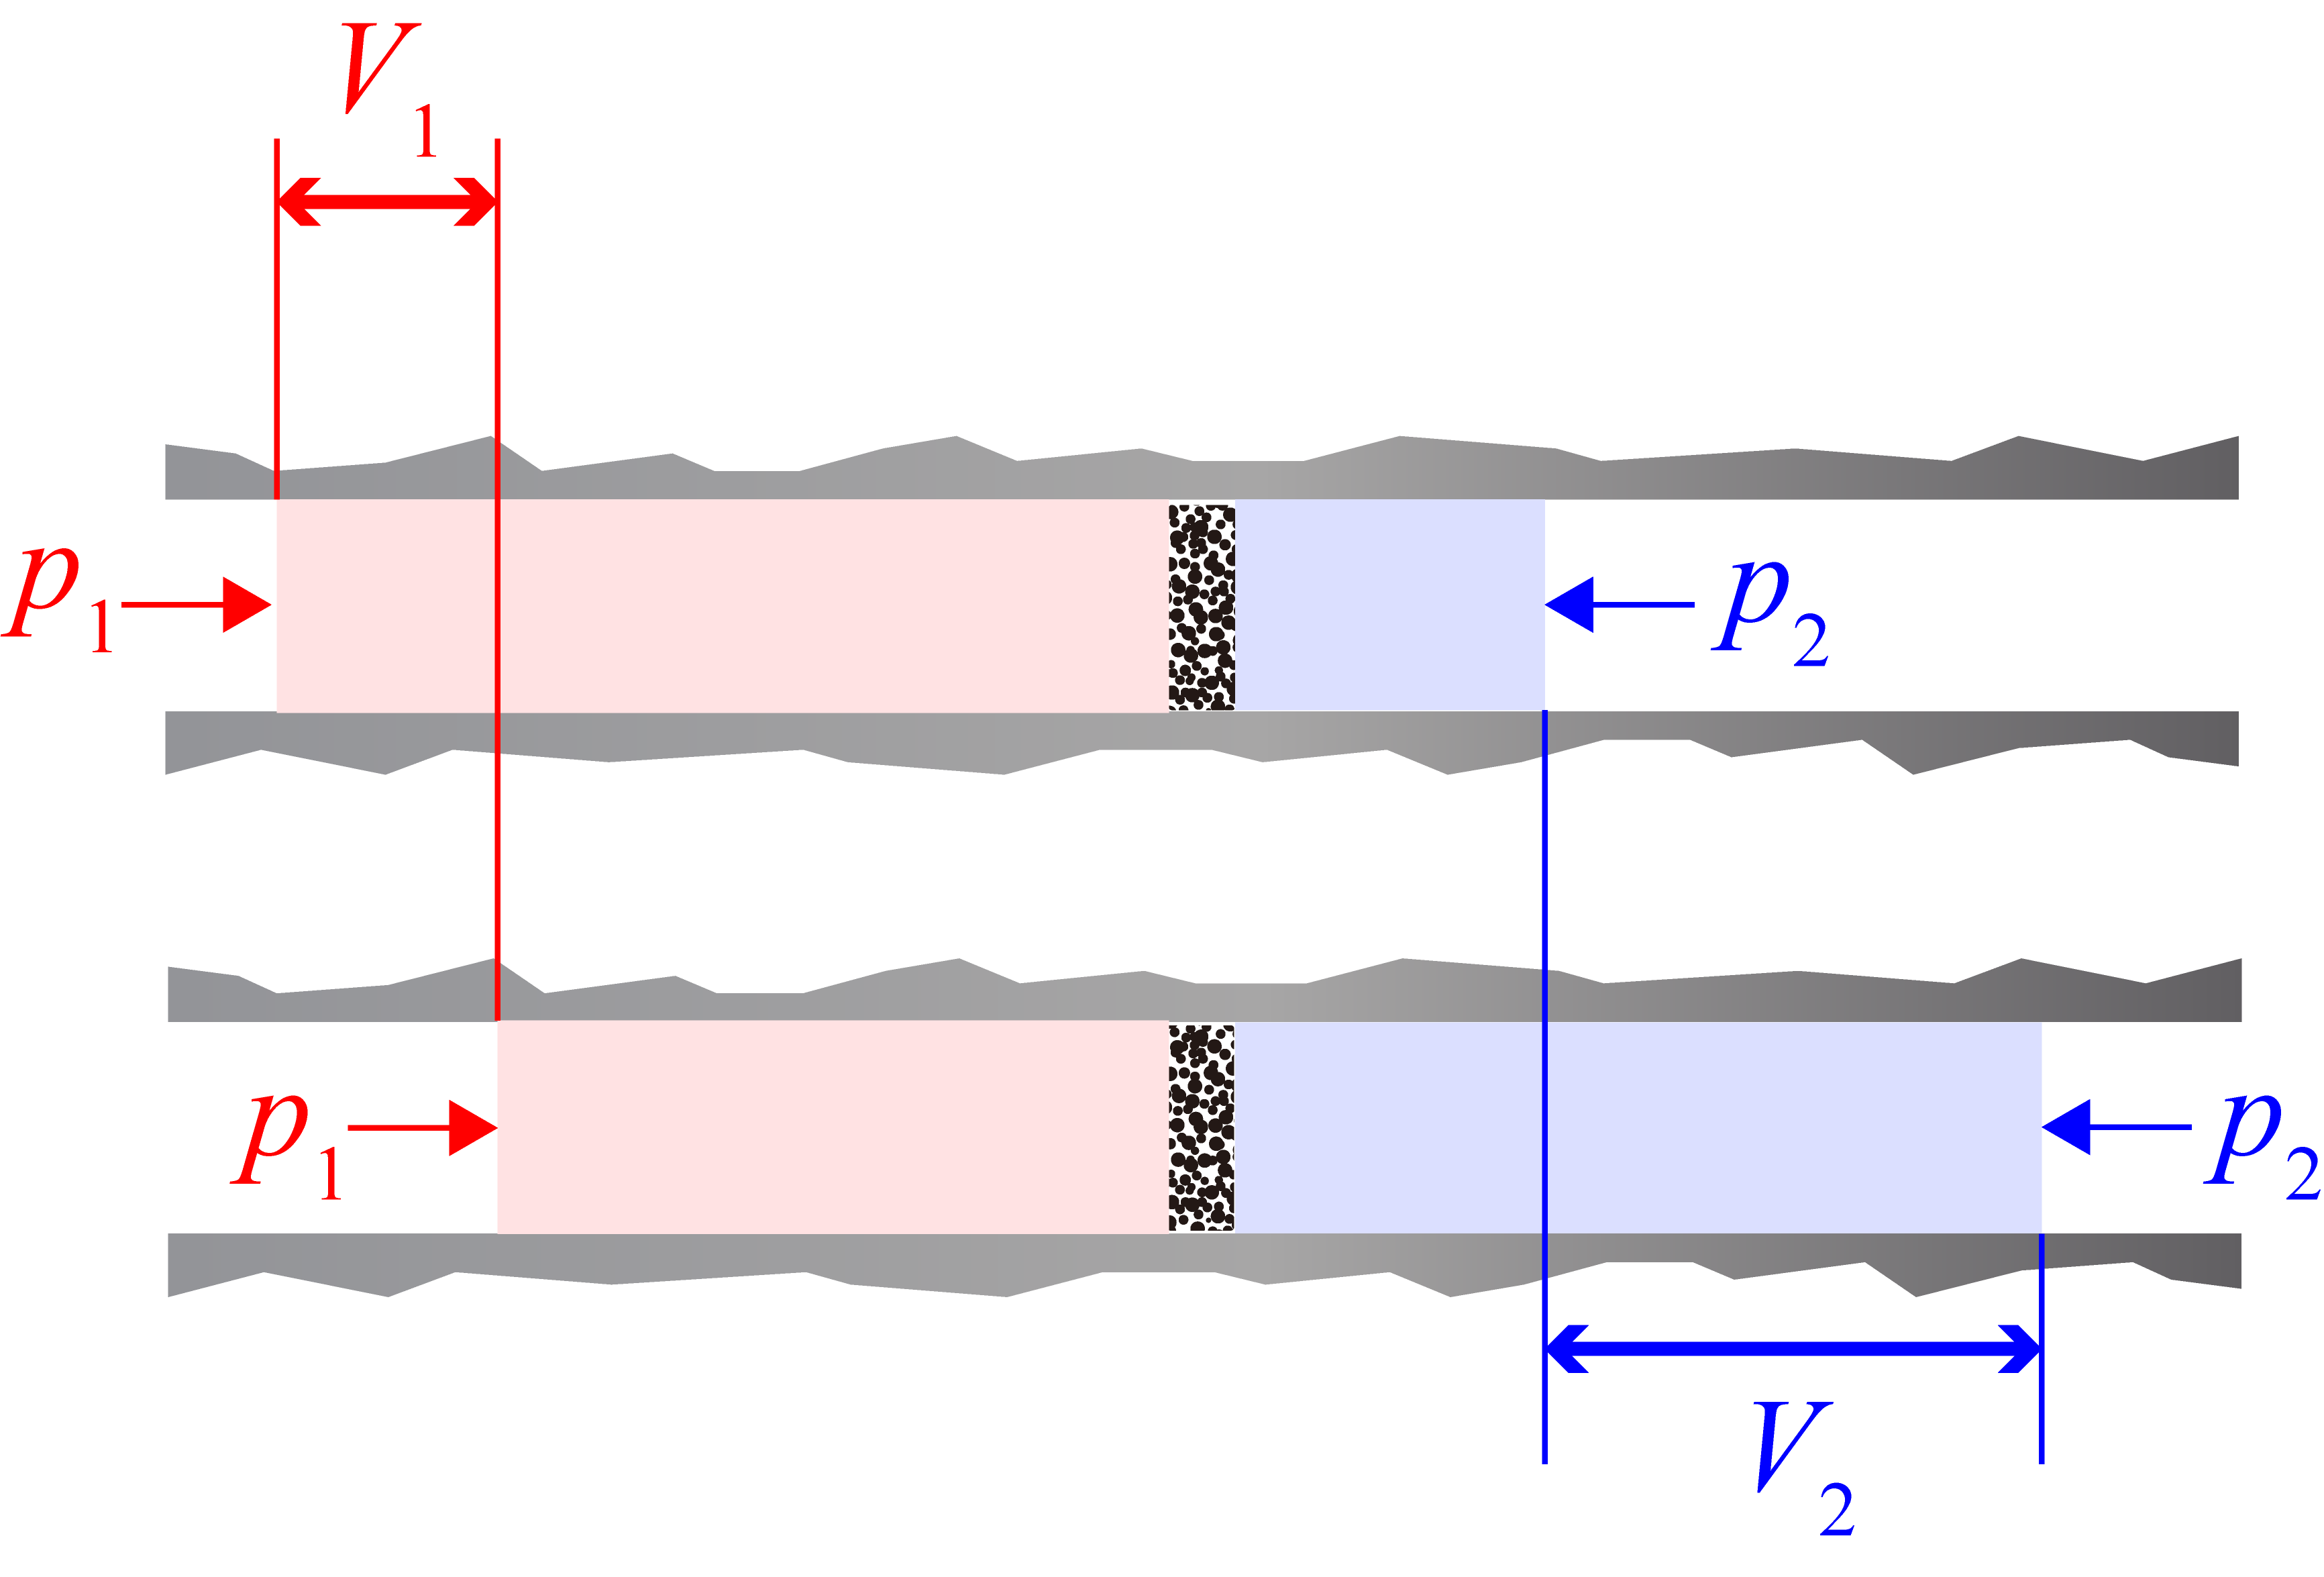
\includegraphics[width=14cm]{image/5-1-9.png}
\caption{多孔塞制节流阀}
\end{figure}

对于红+蓝的整体,\,热一定律表述为:
\[p_1V_1-p_2V_2=U_2-U_1\]

即:
\[U_1+p_1V_1=U_2+p_2V_2\quad ;\quad H_1=H_2\]

也就是说,\,节流过程前后焓不变的过程.\,若流过的气体是理想气体,\,那么
\[H=\nu C_{mV}T+pV=\nu (C_{mV}+R)T=\nu C_{mp}T\]

可见这也是一个温度不变的过程.\,但是吸热,\,做功都为零,\,它并不是一个达到平衡的准静态过程.

\npg{-2cm}

\section{开放系统的理想气体}

开放的气体系统一般有两个特点,\,一是其性质一般被描述为:\,在某处$\bs{r}$的气体性质怎样.\,而描述该气体性质的只能是各种强度量.\,如压强$p(\bs{r})$,\,温度$T(\bs{r})$等等.\,二是气体往往处于动态的物质,\,能量的交换与流动中.\,这就意味着我们分析其物理规律时必须单独取出一个\emph{气团}(parcel of air)作为研究对象.\,研究周围气体对它可能造成的微观扩散,\,黏滞,\,传热过程,\,研究周围气体对气团压力造成的体积功与加速过程.\,下面我们由简入难地分析这些问题.

\subsection{静态平衡问题\ca 重力场中的大气}
对于静态平衡的热力学体系,\,气团首先要符合的是静力学平衡条件:
\[\nabla p+\bs{f}=\bs{0}\]

其中$\bs{f}$代表体积力,\,我们考虑重力场系统,\,则为:
\[\nabla p+\rho \bs{g}=\bs{0}\]

而密度反过来又同时和压强,\,温度有关:
\[\rho=\frac{\mu p}{RT}\]

\begin{wrapfigure}[20]{o}[-10pt]{4cm}
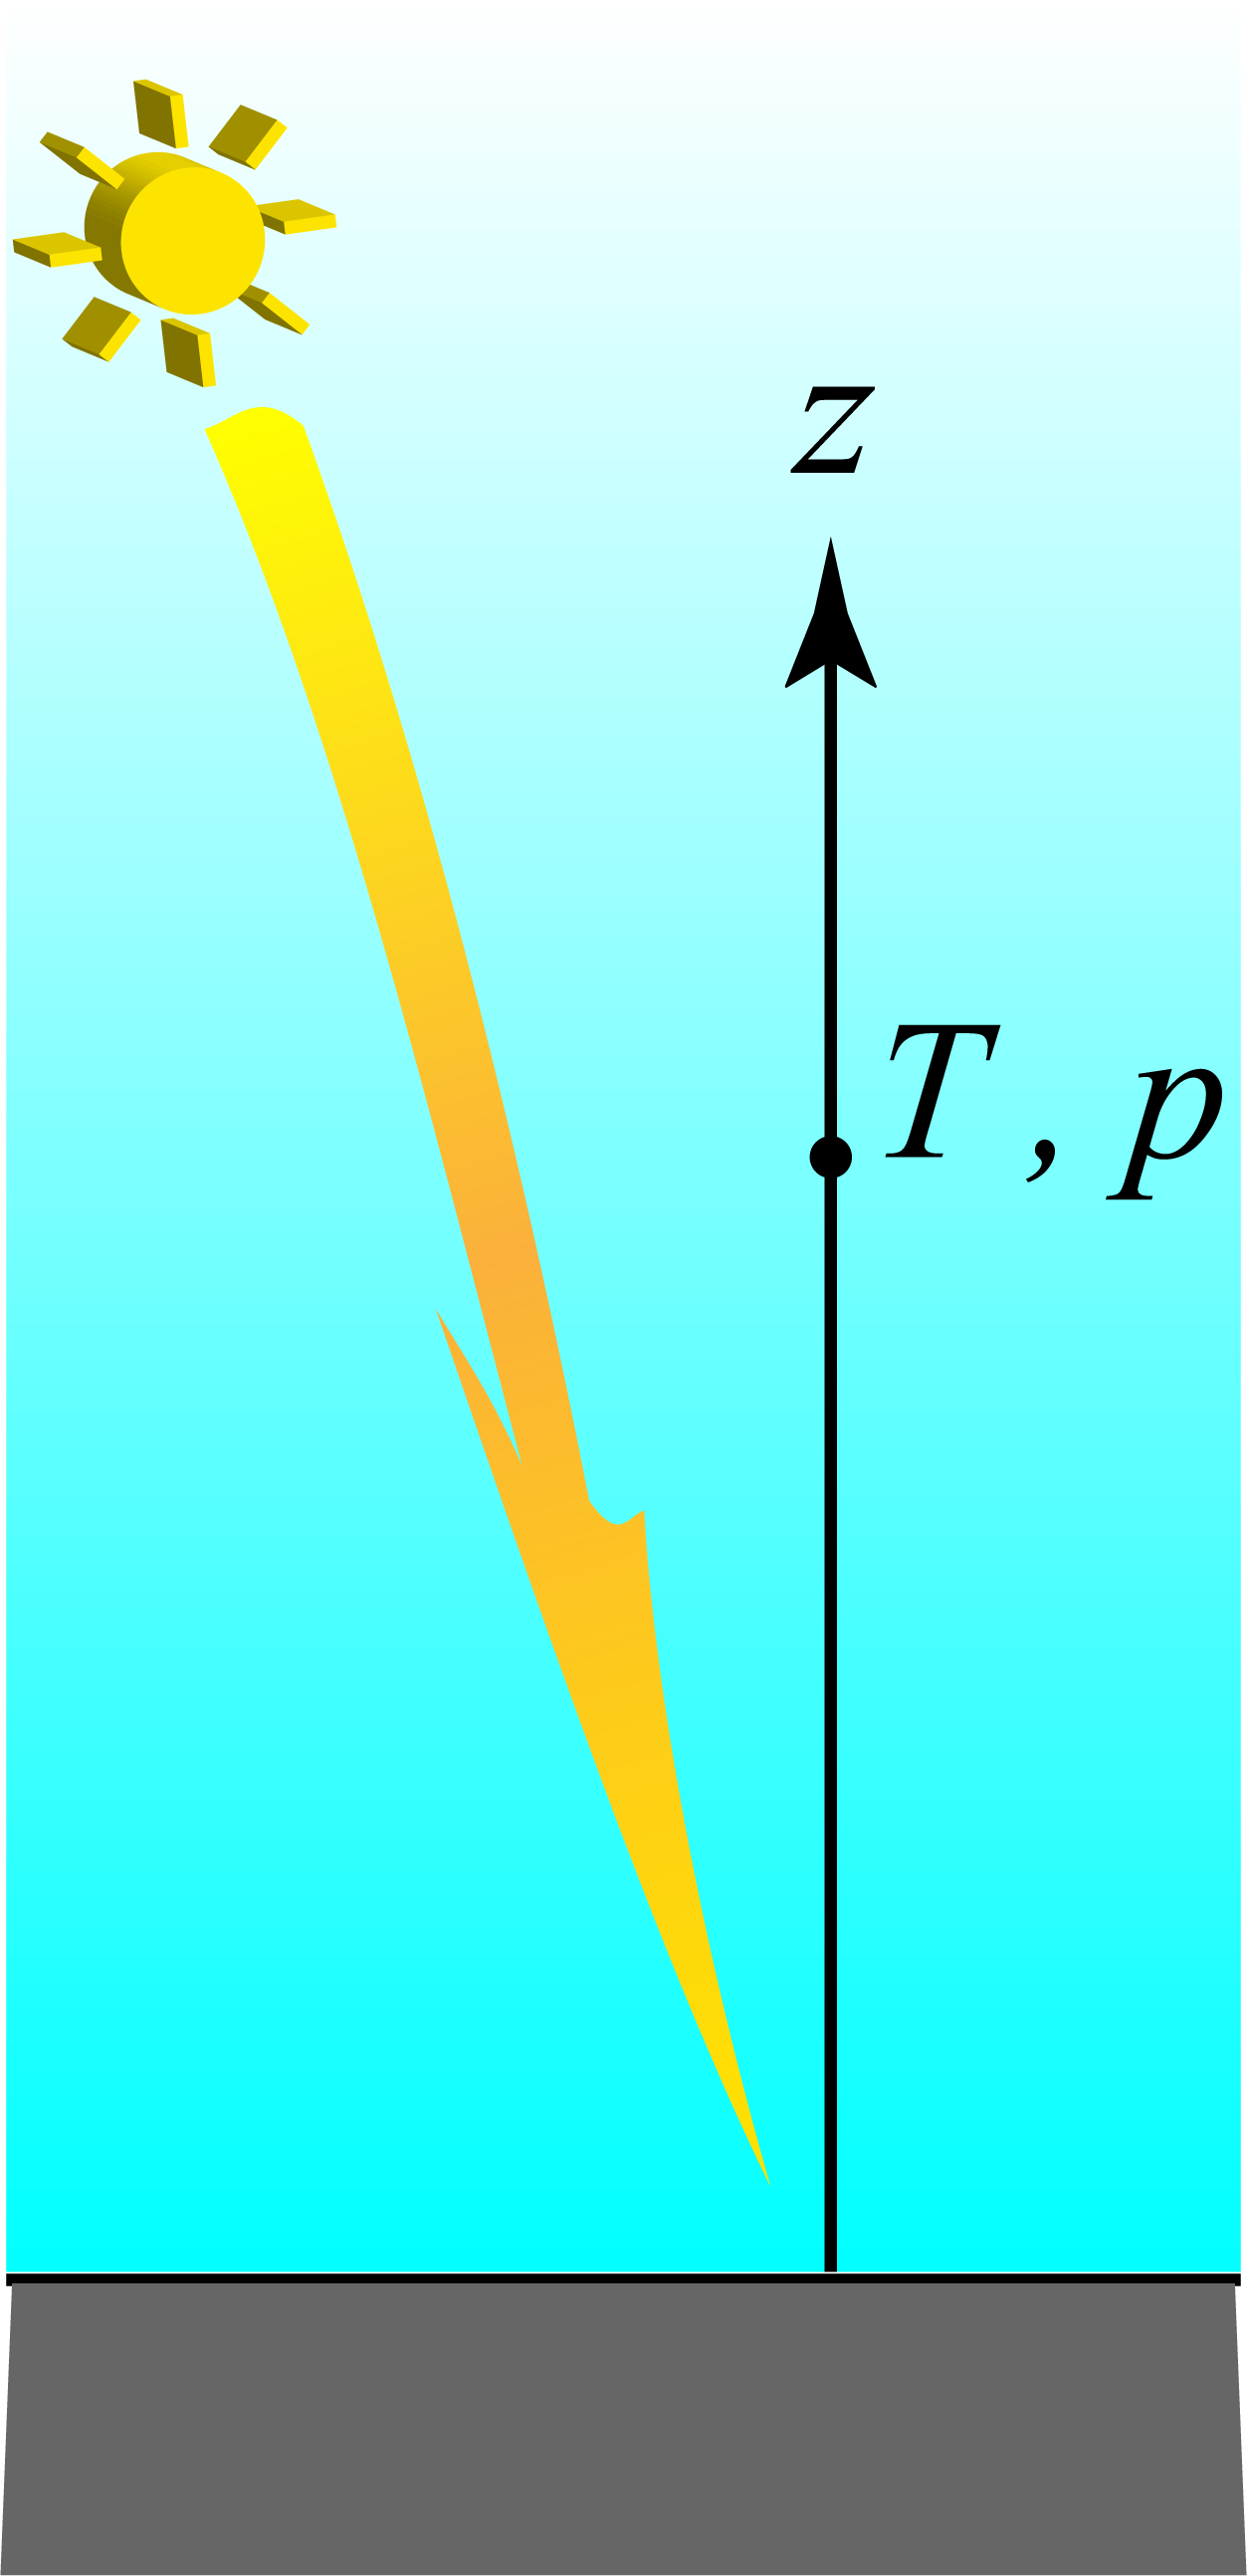
\includegraphics[width=4cm]{image/5-1-10.png}
\caption{地球大气}
\end{wrapfigure}
于是,\,压强的分布纯粹由温度分布决定,\,而温度分布则看似成为了一个纯粹的热学问题,\,而且在一定范围内粗略地研究我们可以简单地假设温度随高度均匀地变化$T(z)=T(0)-\Gamma z$.\,然而这个问题并不简单,\,大体上如果讨论限于地球表面对流层的大气,\,其基本图像可以视为由太阳照射地表,\,地表升温而加热大气导致的.\,而对于不同的气候,\,地理环境,\,时间与天气条件这个温度随高度递减的方式都十分地不相同,\,我们也还是定义\emph{环境温度递减率}(environmental lapse rate)来线性表示温度的降低:
\[\Gamma=-\frac{\ud T}{\ud z} \quad;\quad T(z)=T(0)-\Gamma z\]

了解这一点后便可计算出其压强分布:
\[p(z)=p(0)\cdot[1-\frac{\Gamma z}{T(0)}]^\frac{\mu g}{\Gamma R}=p(0)\cdot[\frac{T(z)}{T(0)}]^\frac{\mu g}{\Gamma R}\]

当环境递减率取某些不同的值时大气的性质是不同的,\,我们考虑其对流性质.\,考虑一个干的气团,\,让它在垂直方向上发生微扰,\,认为力学平衡总是很快地达到\ca 气团压强始终等于外大气压.\,但热学平衡总是来不及达到\ca 既使气团温度与外大气不相等,\,它与外界的热量交换可以忽略,\,从而可以发现,\,气团做绝热碰撞:
\[p(z)=p(0)\cdot[\frac{T'(z)}{T(0)}]^\frac{\gamma}{\gamma -1}\]

比对气团温度$T'(z)$与外大气温度$T(z)$,\,我们发现有一临界的环境温度递减率,\,我们称为\emph{干绝热递减率}(dry adiabtic lapse rate),\,它表征干燥的气团发生微扰后温度,\,密度恰好与周围大气相等的情况:
\[\Gamma_d=\frac{\gamma-1}{\gamma}\frac{\mu g}{R}=\frac{\mu g}{C_{mp}}=9.8\cdgr/\mathrm{km}\]

若$\Gamma>\Gamma_d$,\,则环境递减率过高,\,向上微扰的气团温度高于环境温度,\,所受浮力偏大,\,将偏离平衡位置,\,产生热对流,\,成云致雨.\,反之,\,$\Gamma<\Gamma_d$时浮力偏小,\,气团受到回复力而稳定在平衡位置处,\,对应着稳定无对流的大气.\,对于地球大气体系,\,有对流与无对流的情况都有时发生,\,其平均递减率就在临界绝热递减率附近.

对于临界大气为何温度随高度线性递减,\,而递减率又与定压热容有直接的关联,\,有一种较为直接的证明方法.\,其思想为虚功原理结合下面经常使用的流管分析法.\,我们让从$z=0$到$z=h$的截面积为$A$的气柱在顶部与底部的压力作用下向上发生虚位移,\,由于是临界平衡,\,故位移以后恰巧每一小块气柱$A\ud z$都与新的位置的环境大气性质全同,\,也就是与之前在这儿的那块气柱性质一样.\,整体上看,\,相当于把$z=0$处的一块质量为$\delta m$的气团位移到了$z=h$处.\,写出热力学第一定律,\,要注意其本质为能量守恒,\,这里还要包括重力势能:
\[p(0)\delta V(0)-p(h)\delta V(h)=\delta U(h)-\delta U(0)+\delta m gh\]

而由焓的定义$\delta H=\delta U +p\delta V$,\,以及理想气体的焓有公式$\delta H=\delta \nu C_{mp}T$,\,我们得出:
\[\delta \nu C_{mp}[T(0)-T(h)]=\delta \nu \mu gh\]

即:
\[T(h)=T(0)-\frac{\mu g}{C_{mp}}h\]

对于实际地球对流层大气来说,\,还需要考虑空气中水蒸气受冷造成的液化放热现象,\,其临界递减率将会取决于气体含水蒸气的多少.\,而地球下层大气还分为\emph{对流层}(troposphere)与\emph{平流层}(stratosphere),\,平流层含大量臭氧,\,太阳的紫外辐射将在传播的过程中被平流层逐渐吸收.\,所以平流层的上部具有较强的辐射和较高的平衡温度,\,而温度随高度递增,\,提供了一个稳定的大气环境,\,极难发生对流.





\subsection{能量守恒\ca 伯努利方程}
我们把流体力学里讨论的\emph{伯努利方程}(Bernoulli Equation)推广到热力学中.\,它适用条件为\emph{定常流动}(steady flow)中的同一条\emph{流线}(streamline)上.\,它也是推广的热力学第一定律,\,它代表能量的守恒.

\begin{wrapfigure}[10]{o}[-10pt]{6cm}
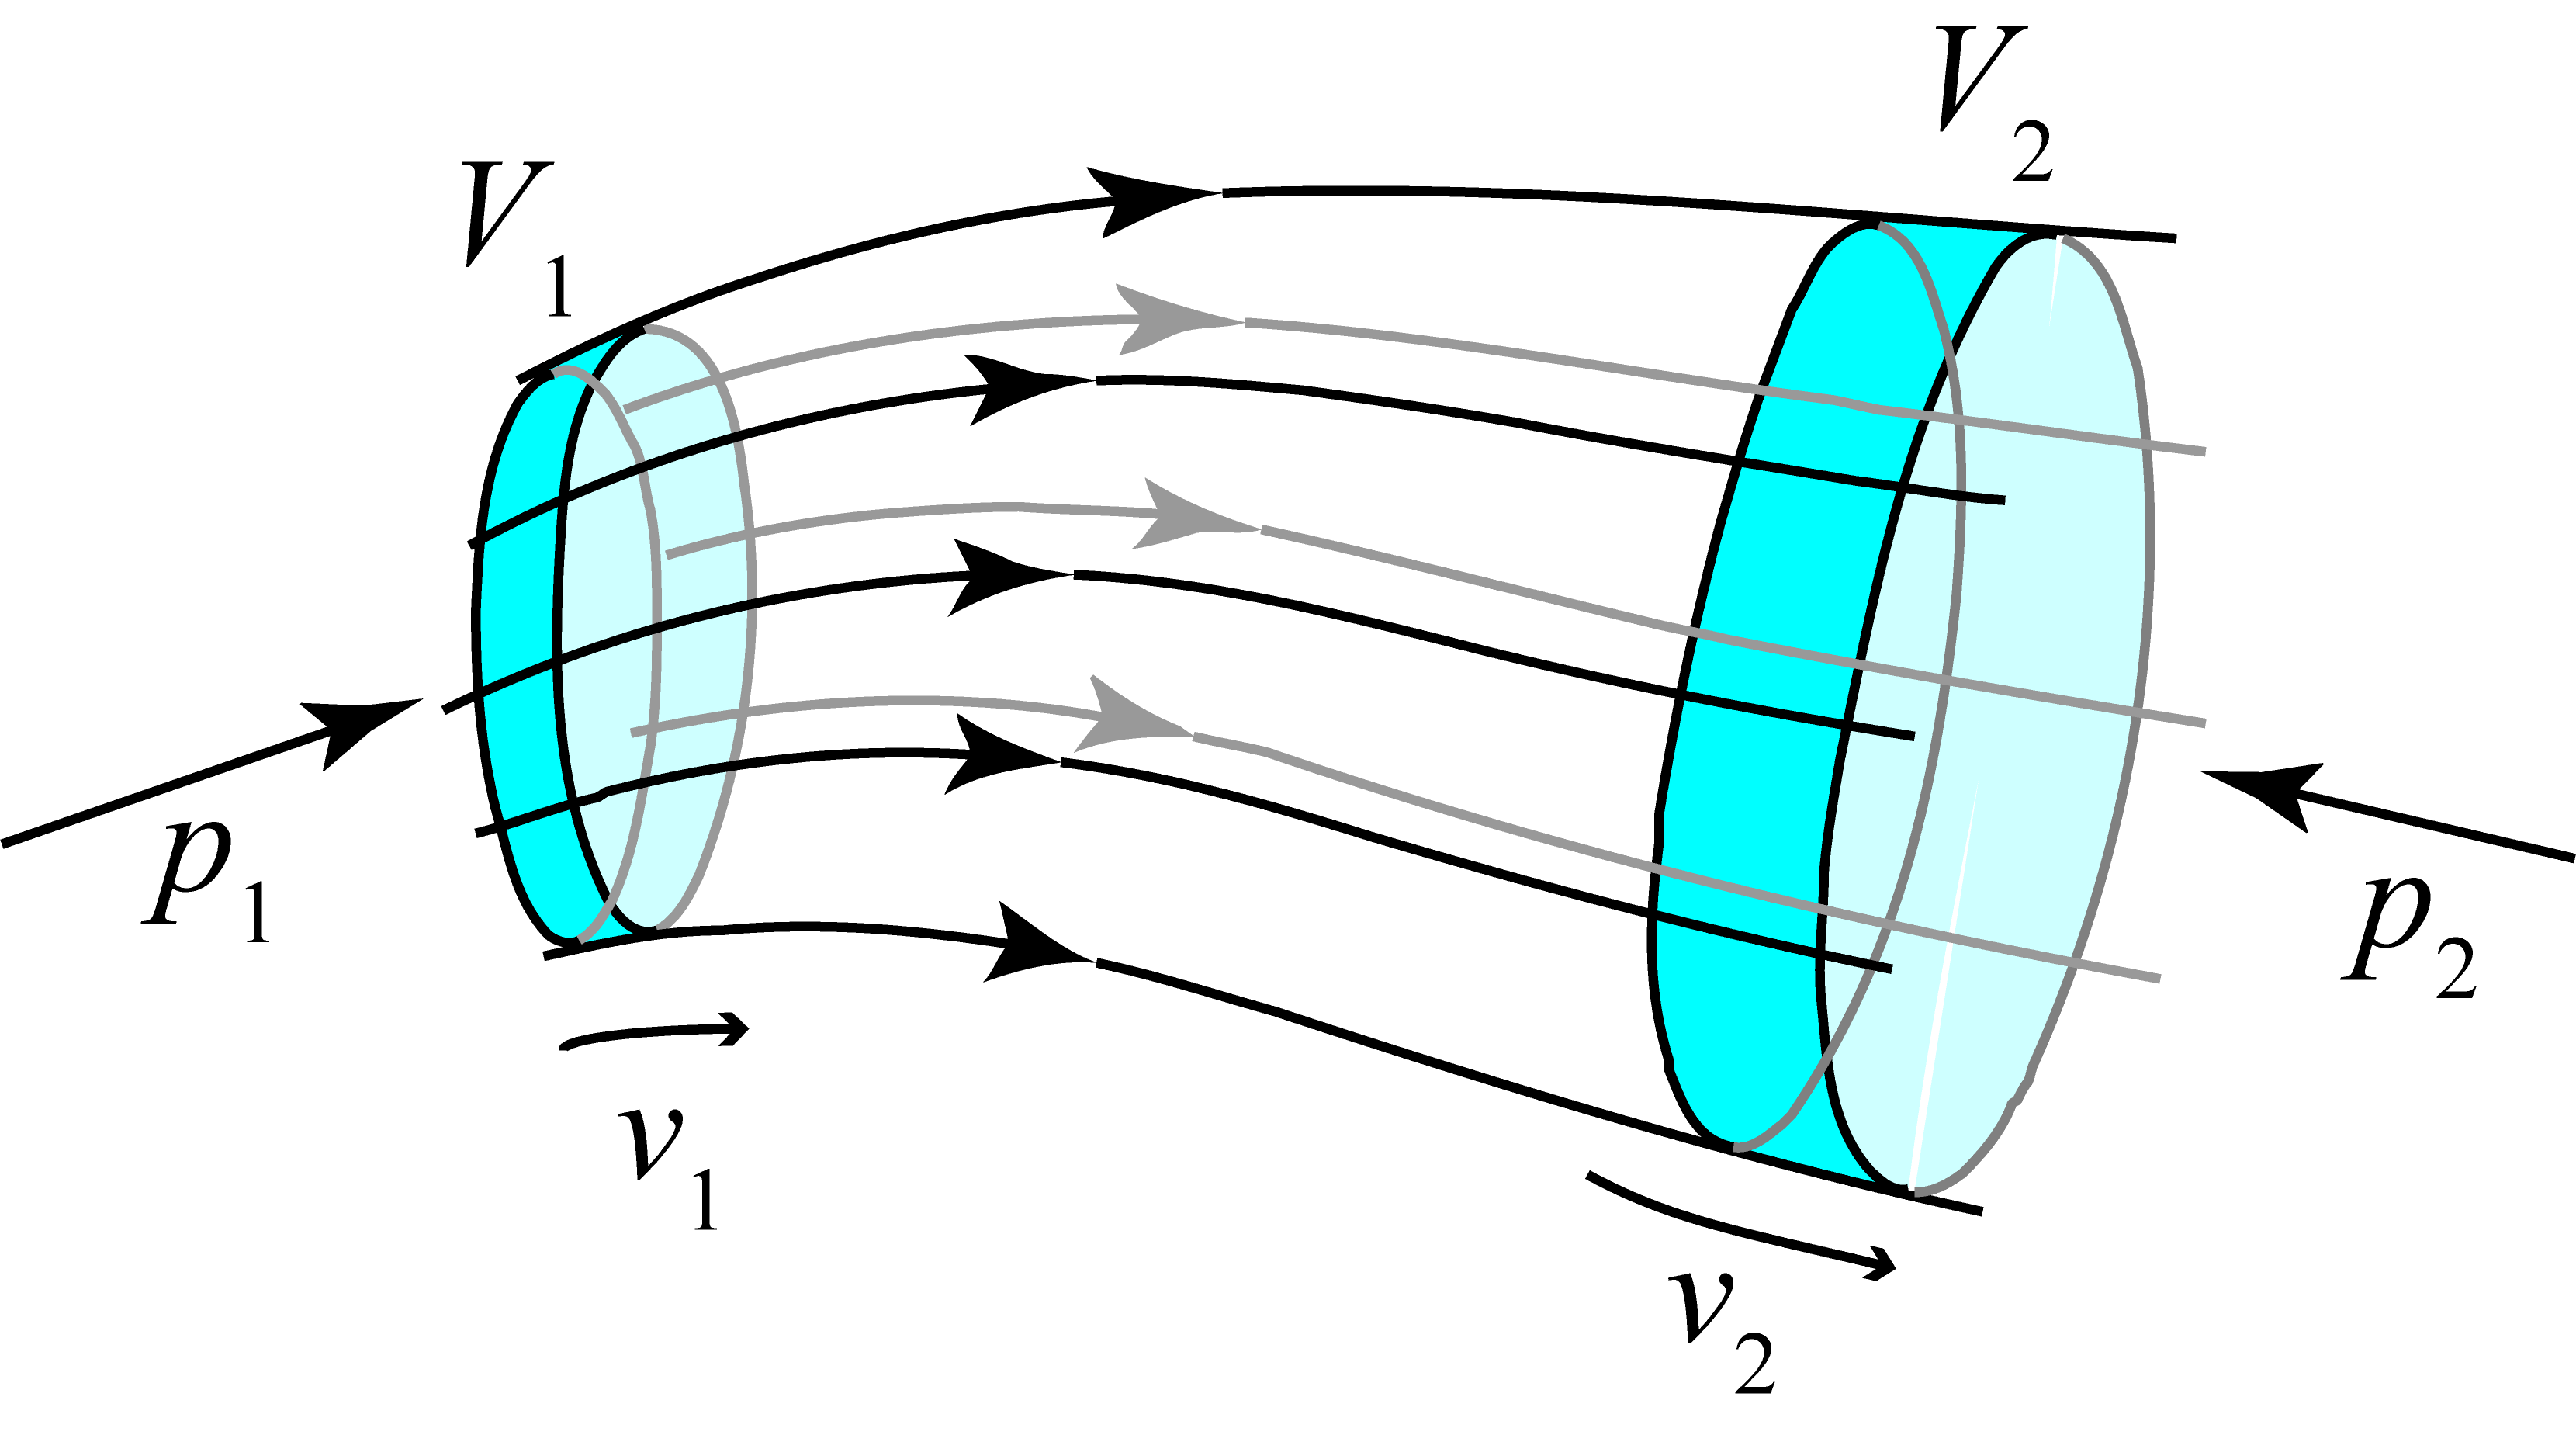
\includegraphics[width=6cm]{image/5-1-11.png}
\caption{气体沿一条流管流动}
\end{wrapfigure}
不可压缩流体的伯努利方程的图像其实很清晰,\,我们若不考虑流体势能的变化,\,那么伯努利原理实际是在说,\,两侧的压强差导致了流体的加速:
\[p_1-p_2=\frac{1}{2}\rho v_2^2-\frac{1}{2}\rho v_1^2\]

从而沿流线,\,以下量守恒:
\[p+\frac{1}{2}\rho v^2=\mathrm{const.}\]

但若考虑可以压缩的气体,\,以及考虑保守外力的做功,\,是否有以上守恒量呢?\,我们假设保守外力为质量力:\,单位质量的流体的势能为$\Phi$,\,那么对于一定时间间隔$t$下的流管发生的流动$m=Qt$,\,有以下能量守恒:
\[p_1V_1-p_2V_2=(U_2+\frac{1}{2}mv_2^2+m\Phi_2)-(U_1+\frac{1}{2}mv_1^2+m\Phi_1)\]

两边同时除以质量,\,得守恒律:
\[u+\frac{p}{\rho}+\frac{v^2}{2}+\Phi=\mathrm{const.}\]

其中$u+p/\rho=u+pv=h$即为比焓,\,而$u$为比内能,\,$v$为比体积,\,``比''表示单位质量的某物理量,\,它是一种强度量.\,从而以上量我们还可以写为:
\[h+\frac{v^2}{2}+\Phi=\mathrm{const.}\]

我们还定义所谓的\emph{阻滞焓}(stagnation enthalpy)的概念.\,它表示让运动的气体发生某种虚构的定常流动绝热地停止下来后气体应该有的焓.\,那么比阻滞焓为:
\[h'=h+\frac{v^2}{2}\]

最后这一广义的伯努利方程,\,就被我们写为一个广义的两项的能量守恒形式:
\[h'+\Phi=\mathrm{const.}\]

那么对于理想气体,\,我们还可以定义阻滞温度:
\[T'=T+\frac{\mu v^2}{2C_{mp}} \quad ; \quad h'=\frac{1}{\mu}C_{mp}T'\]

而对于普通不可压缩流体,\,我们一般不关心其热学性质,\,故焓可以扣除内能项$h=p/\rho +v^2/2$,\,而$\rho$为常数.\,这样我们又可以定义阻滞压强:
\[p'=p+\frac{1}{2}\rho v^2\quad;\quad h'=\frac{p'}{\rho}\]




\subsection{动量守恒\ca 欧拉方程}
让我们考虑管道内的理想气体流动,\,管道的截面积在不断减小的情况$A=A(x)$.\,可以想见,\,这会导致流速的增加,\,进一步导致压强的减小,\,对应方程为\emph{连续性方程}(continuity equation)与伯努利方程,\,分别对应质量与能量守恒:
\[\rho vA=\mathrm{const.}\]
\[\frac{1}{\mu}C_{mp}T+\frac{v^2}{2}=\mathrm{const.}\]

以上方程还应联系物态方程理解:
\[\rho=\frac{\mu p}{RT}\]

\begin{figure}[H]
\centering
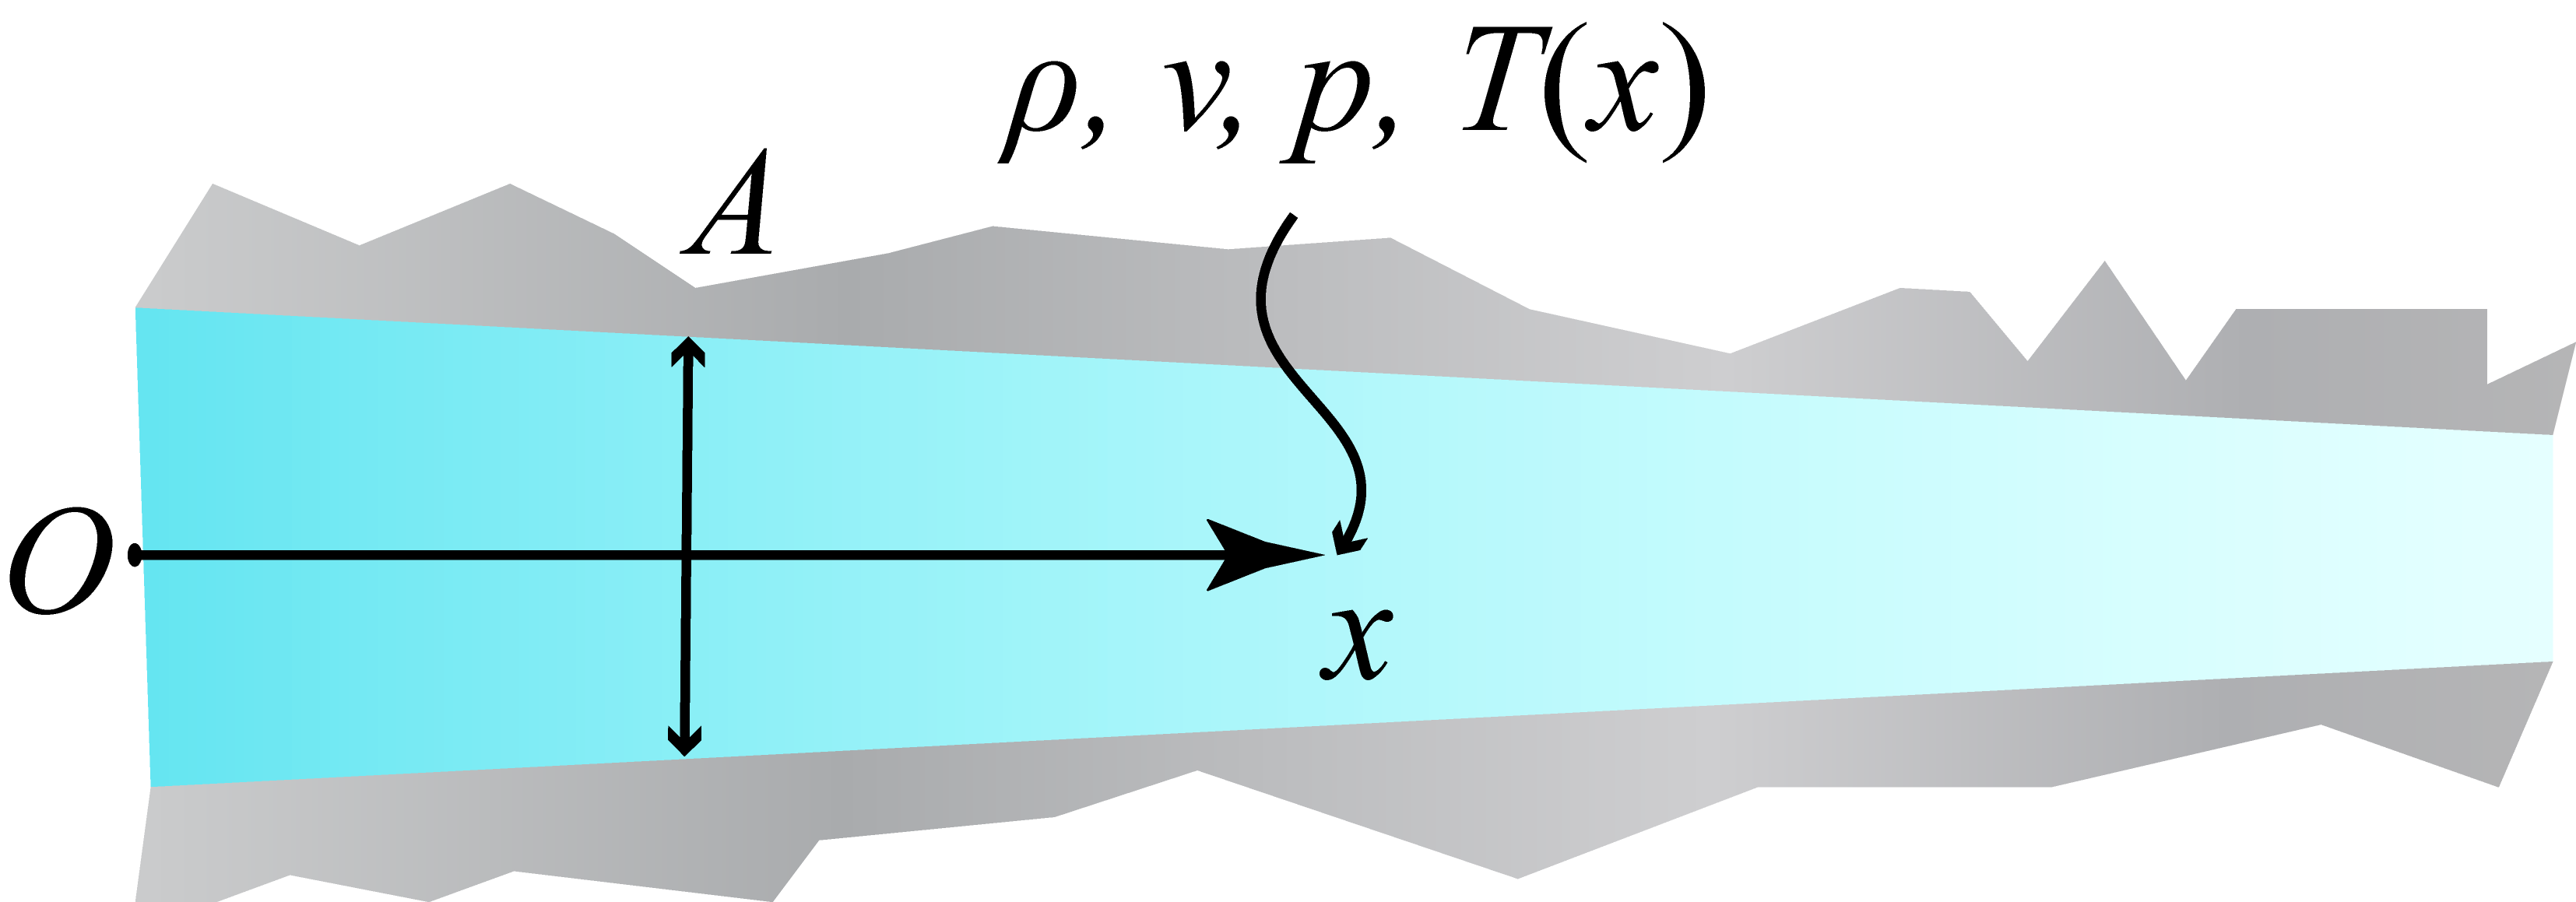
\includegraphics[width=12cm]{image/5-1-12.png}
\caption{截面积减小的管道内的气流}
\end{figure}



注意到我们把$A$的变化当做已知量以后,\,却仍设了待求解的四个物理量$v(x),\,p(x),\,T(x),\,\rho(x)$,\,但目前却只有三个方程.\,那么我们漏了怎样一个方程呢?\,这个方程就是流体的\emph{欧拉方程}(Euler equation),\,它是一个纯粹的动力学方程,\,不包含任何热效应.\,一般写作:
\[\frac{\mathrm{D} \bs{v}}{\mathrm{D} t}=-\frac{\nabla p}{\rho}-\nabla \Phi\]

其中$\mathrm{D}$代表\emph{随体导数}(material derivative):
\[\frac{\mathrm{D}}{\mathrm{D} t}=\frac{\ud}{\ud t}+\bs{v}\cdot \nabla\]

上式代表了压强梯度力与保守外力对流体的加速效应,\,在上述情形中没有外力所以等式右边只有一项.\,实际上,\,它代表了整个体系动量守恒.\,而对于上述情形,\,气体做定常流动,\,上式写为:
\[v\frac{\ud v}{\ud x}=-\frac{1}{\rho}\frac{\ud p}{\ud x}\]

这一个式子也可以由上一节的类似方法\ca 取一定长度的气团来导出.\,但切不可忽略管壁对气体在过程中作用的冲量:
\[p_1A_1\bs{e}_x \cdot t-p_2A_2\bs{e}_x \cdot t+\int -p\ud \bs{A} \cdot t=m\bs{v}_2-m\bs{v}_1\]

左边恰巧是在整个表面的压强的面积分,\,可以由高斯定理化为体积内的体积分:
\[\int_{x_1}^{x_2}-\frac{\ud p}{\ud x}\cdot A\ud x=Q(v_2-v_1)\]

又考虑到以上积分式无法直接积出结果,\,故对积分上限求导,\,再考虑到$Q=\rho vA$,\,化简后即得欧拉方程:
\[\frac{\ud p}{\ud x}=-\rho v\frac{\ud v}{\ud x}\]

对于管道截面积相对于长度变化缓慢的情况\footnote{即,\,在所关心的范围内截面积的相对变化很小:\[\frac{\Delta A}{A}\ll 1\]},\,联立以上四个方程,\,解得:
\[\frac{\ud v}{v}=-\frac{\ud A}{A}(1-\frac{\mu v^2}{\gamma RT})^{-1}\]
\[\ud p=\rho v^2\cdot\frac{\ud A}{A}(1-\frac{\mu v^2}{\gamma RT})^{-1}\]
\[\ud T=\frac{\mu v^2}{C_{mp}}\cdot\frac{\ud A}{A}(1-\frac{\mu v^2}{\gamma RT})^{-1}\]

可见,\,随着截面积$A$的减小,\,流速加快,\,压强和温度都要减小,\,利用这个效应可以制作纯粹依靠风力制冷的``土空调''.\,注意到以上结论还依赖于一个条件:
\[\frac{\mu v^2}{\gamma RT}<1\]

这意味着分子代表的气团集体运动能量要远小于分母代表的微观热运动能量,\,这在一般情况下是很容易满足的,\,因为$v\sim 10 \mathrm{m/s}$而热运动平均速率$\bar{v}\simeq 500 \mathrm{m/s}$,\,若对于高速运动的气体,\,其发生的过程中气团速度的改变与热运动平均速度可以比拟,\,实际上把气团处理为平衡的理想气体也是不妥当的.
%!TEX root = ../physical-olympics-2.tex
\chapter{热力学第二定律}


热力学第一定律固然强大,\,它根本上杜绝了所谓的\emph{第一类永动机}(perpetual motion machine of the first kind)的可能性,\,也排除了一大类不现实的热力学过程的发生.\,然而由这样一个只关心整体性质,\,不深入到微观本质的热力学规律又能告诉我们多少呢?\,\emph{炼金术}(alchemy)不违背热力学第一定律,\,它企图实现物质与物质之间的随意转化,\,\emph{第二类永动机}(perpetual motion machine of the second kind)亦不违背热力学第一定律,\,它基于能量守恒,\,主张同一份能源的无限再生利用.\,对于前者,\,微观机理彻底地否定了它,\,不同的原子有不同的构成,\,原子核的结构十分稳定,\,至今无法自由操控.\,而对于后者,\,统计规律也彻底地进行了否定,\,它告诉我们,\,一个体系的过程总是有确定的方向性,\,在一定条件下,\,过程被我们分类为\emph{自发过程}(spontaneous process)与\emph{不自发过程}(non-spontaneous process),\,具有特定方向性的过程一旦发生,\,其时间反演的过程就将不现实.\,但十分神奇的一点是,\,不同体系的不可逆特性居然是紧密相关的,\,若将一个过程的不可逆性与另一个不可逆过程的不可逆性建立联系,\,我们就能从中同时发现统一的热力学温标与态函数熵这两个概念,\,从而量化过程的不可逆性,\,这一套宏观的规律称为热力学第二定律.\,它道出了热力学过程的方向性,\,本质是微观统计规律,\,限制了另一大类不现实的热力学过程的发生.


\section{循环过程}
在历史上,\,热力学基本规律的确立与发展和热机的使用与改进是紧密相关的.\,直到今天卡诺循环的引入仍然不失为介绍热力学第二定律理论体系的强有力工具.\,本节将介绍热机,\,热泵的基本模型与著名的卡诺循环.\,为之后引入热力学第二定律相关概念打下基础.

\subsection{热机与热泵}
\begin{wrapfigure}[13]{o}[-10pt]{7cm}
\centering
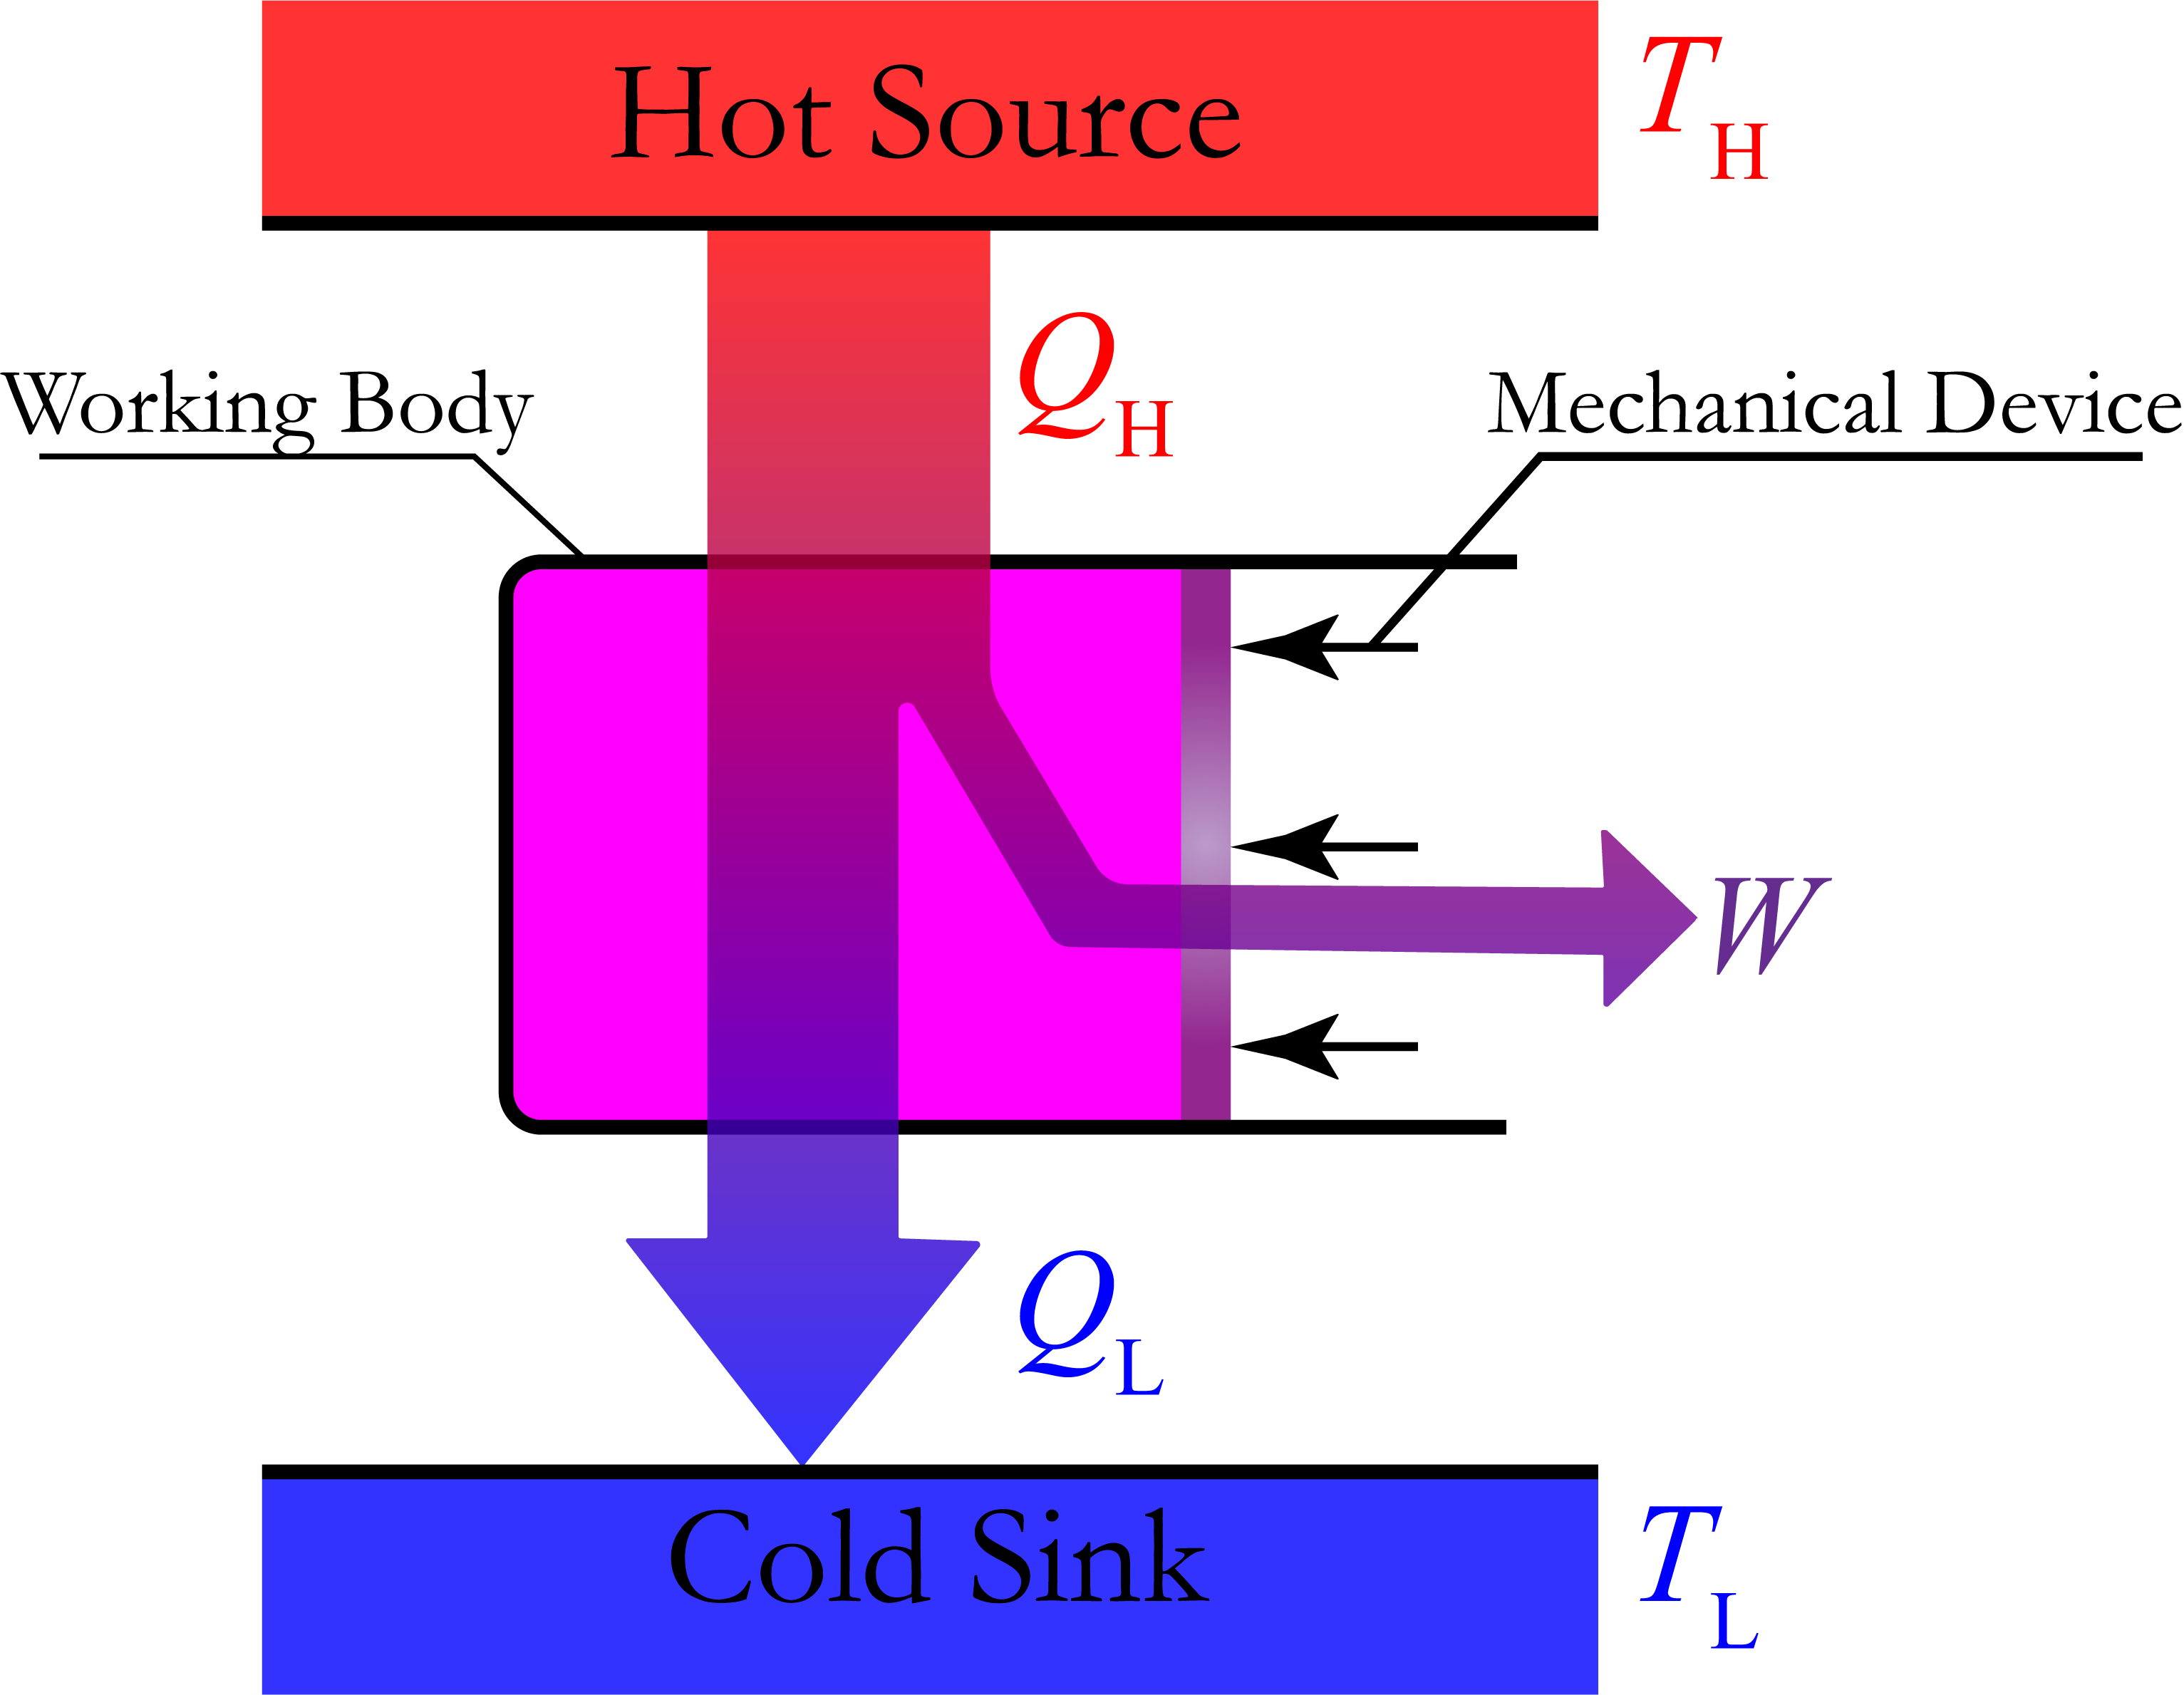
\includegraphics[width=7cm]{image/5-2-1.png}
\caption{热机模型}\label{fig:heat engine}
\end{wrapfigure}
上一章介绍过循环过程的概念.\,我们介绍了$p-V$系统的正负循环.\,现在我们把这样的$p-V$体系看成很多实际生活中一些机器的工作过程的抽象.\,其实际承担了状态循环变化的体系称为\emph{工作物质}(working body).\,而其联动的\emph{机械装置}(mechanical device)可以与外界交换功.\,最后,\,这样的体系还需要可以与其交换热量的对象,\,凡是工作物质从中吸热的被称为\emph{热源}(heat source),\,而工作物质向之放热的被称为\emph{冷库}(cold sink).\,这样我们就抽象出了一个理论模型,\,根据热力学第一定律,\,如果做正循环,\,工作物质一个循环将从高温热源吸收更多的热量,\,向低温冷库放更少的热量,\,而通过机械装置输出功,\,故被称为\emph{动力循环}(power cycle),\,对应机器为\emph{热机}(heat engine).\,而如果考虑相反的过程\footnote{这样的过程不一定可逆,\,这里指的是那些定性现象相反的循环.},\,工作物质一个循环向高温热源放热,\,从低温冷库吸热,\,机械装置要对它做功,\,则是一个\emph{泵热循环}(heat pump cycle).\,对应机器被称为\emph{热泵}(heat pump).

\begin{figure}[H]
\centering
\includegraphics[width=14cm]{image/5-2-2.jpg}
\caption{俄罗斯巴拉科沃(Balakovo)核电站汽轮机}
\end{figure}

根据以上原理,\,热机主要分为以下两大类:
\begin{description}
	\item[\hei 蒸汽机(steam engine)]  蒸汽机是一类\emph{外燃机}(external combustion engines),\,工作物质是在气相与液相混合的水(水蒸气).\,用外界燃烧的热量,\,或者来自太阳能,\,核能,\,地热等的非燃烧热量加热\emph{锅炉}(boiler)中的水,\,由此产生高温高压蒸汽,\,用蒸汽带动机械装置运转向外输出能量.\,经过这样的装置后(这中间一般视为节流过程),\,水蒸气一般变为过饱和的冷气体或者还夹杂着水滴,\,进一步导入冷凝器而液化变为液态水回收进入锅炉.\,完成一个循环.\,18世纪末与大半个19世纪可谓``蒸汽时代'',\,蒸汽机在大型机械生产工厂,\,蒸汽机车,\,蒸汽机轮船等交通工具中大放异彩.\,虽然石油开采为小型汽车生产提供了可能,\,大型交通工具和生产业动力来源之后也慢慢地几乎被内燃机与电力所取代.\,但直到今天,\,我们的生产生活有$90\%$以上的电量都来自于\emph{汽轮机}(steam turbine)形式的热电厂.\,值得一提的是其中化石能源(煤电,\,气电,\,以及较为小规模的油电)仍然占据$75\%$的高比重(中国与美国的情况大致相同),\,新型能源的比重不大,\,但在稳步上升中.
	\item[\hei 内燃机(internal combustion machine)]  蒸汽机的锅炉设计让燃烧能量给了流动的工作物质,\,实现了工作物质不含燃料,\,不与燃料混合或被燃料污染.\,这有效地提高了燃料能量利用的效率.\,然而却需要为工作物质准备额外的空间,\,不利于把热机做小.\,与之相反,\,内燃机利用了\emph{燃烧室}(combustion chamber)的设计,\,工作物质直接是高能量密度的燃料和氧化剂(一般就是空气).\,利用高温高压下点燃化学反应释放的巨大化学能来产生热,\,导致气体反向对机械装置\ca \emph{活塞}(piston)或\emph{涡轮}(rotor)做功.\,与外燃机工作物质发生的真循环过程不同,\,内燃机发生的过程是一种开放循环.\,以常规的四冲程活塞式内燃机为例,\,气体经历四个冲程:\,\emph{吸入}(intake),\,\emph{压缩}(compression),\,\emph{做功}(power),\,\emph{排出}(exhaust).\,整个循环从常态燃料中开始,\,最后以排出气体在大气中冷却结束.\,而\emph{燃气涡轮发动机}(gas turbine engine)更是针对四个阶段分别设计功能区,\,使得四个阶段同时进行,\,提供了极大的功率输出.\,按照其机械装置的不同分为四类:\,军用战斗机往往采用\emph{涡喷发动机}(turbojet engine),\,而民航客机往往是\emph{涡扇发动机}(turbofan engine);\,运输机,\,巡逻机经常采用\emph{涡桨发动机}(turboprop engine);\,而直升机和其他陆上,\,海上交通工具则通过\emph{涡杆发动机}(turboshaft engine)将动力用传动轴导出.\,在这样的设计中,\,燃料产生的能量用来驱动涡轮带动整个装置大量吸入外界空气\footnote{火箭除外,\,它需要自备燃料与氧化剂.}并有效地压缩气体从而产生动力.\,涡轮转动的能量也正是很多民航飞机上电力的来源.
\end{description}
\begin{figure}[H]
\centering
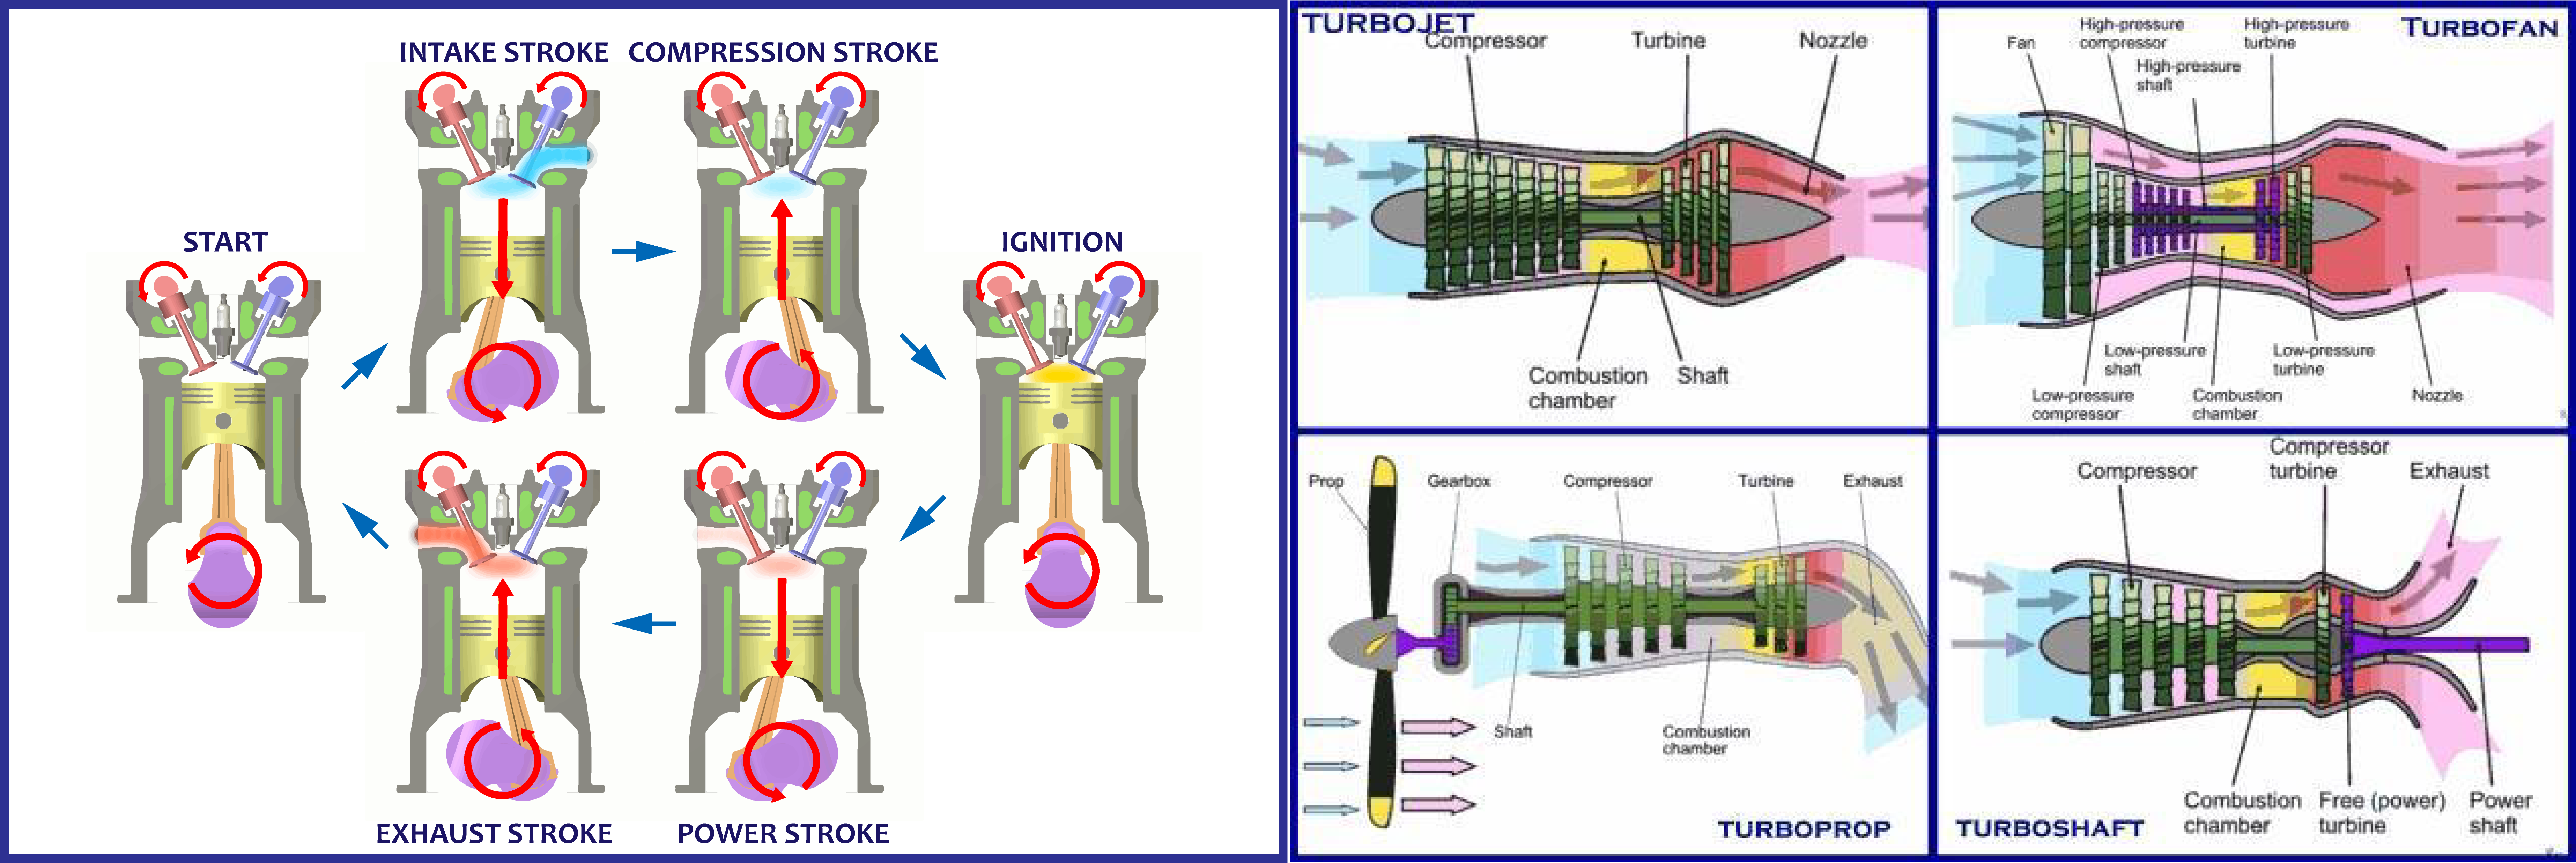
\includegraphics[width=17cm]{image/5-2-3.png}
\caption{左:\,四冲程活塞内燃机;\,右:\,四类涡轮机}
\end{figure}

我们发现,\,将实际的热机抽象为前图\ref{fig:heat engine}那样的模型往往是过分地简单了.\,实际问题中的工作物质往往成分在发生改变,\,有物质的输入输出,\,甚至无法视为一个完整的循环过程.\,但理论可以帮我们分析与把握这个过程的一些主要信息.\,在实际问题中热机的\emph{能效}(energy efficiency)是主要的关心因素之一,\,它定义为输出的有用功$W$与燃料提供的化学能$Q_{\rm H}$之比:
\[\eta=\frac{W}{Q_{\rm H}}\]

\begin{wrapfigure}[22]{o}[-10pt]{7cm}
\centering
\includegraphics[width=7cm]{image/5-2-4.png}
\caption{热泵的普遍构成}
\vspace{1cm}
\includegraphics[width=7cm]{image/5-2-5.png}
\caption{热泵的工作循环}
\end{wrapfigure}
而热泵也根据其设计功能分为\emph{制冷机}(cooling machine),\,\emph{制热机}(heating machine)与\emph{可逆机}(reversible machine).可逆的热泵同时具备制冷制热两种功能,\,采用换向阀来控制气流的流向从而改变效果.\,当采用制热模式时,\,其效率往往比使用单独的电阻加热高3到4倍.

无论何种类型的热泵,\,其构成与原理可以被抽象为典型的四步.\,高温热源处更高温的气体在\emph{冷凝器}(condenser)处变为液态而放热;\,\emph{膨胀阀}(expansion valve)处的节流过程使液态流体温度与压强大降而成为气液混合的状态;\,低温冷库处稀薄的半液态流体在\emph{蒸发器}处蒸发吸热;\,最后通过\emph{压缩机}(compressor)泵入冷凝管,\,压强与温度显著升高.\,这样的循环称为\emph{斯特林循环}(Stirling cycle).


而对于热泵的\emph{性能系数}(coefficient of performance),\,需要对两种不同的模式区分:

对于制冷模式,\,取低温冷库处吸热比输入功率:
\[\eta=\frac{Q_{\rm L}}{W}\]

对于制热模式,\,取高温热源处放热比输入功率:
\[\eta=\frac{Q_{\rm H}}{W}\]

两者都可能大于一.

\subsection{热机循环}
从瓦特({\it Watt}\,)改良蒸汽机开始,\,一代代的工程师开始致力于提高热机的效率.\,这其中便产生了大量实用的热机模型.\,直到1824年法国物理学家与工程师卡诺({\it Carnot}\,)给出了惊人的卡洛热机模型与关于热机工作效率上限的论断.\,这实际上意味着\emph{热力学}(thermodynamics)的诞生.\,之后热机优化建立在严格的热力学计算的基础上.\,发展到今天理论早已成熟,\,只待技术的发展与革新.

简单的热机循环计算往往将工作物质视为理想气体在$p-V$图上的准静态过程构成的循环.\,下将一一列举:
\subsubsection{\hei 勒鲁瓦循环(Lenoir cycle)}
\begin{wrapfigure}[11]{o}[-10pt]{5cm}
\centering
\includegraphics[width=5cm]{image/5-2-6.png}
\caption{Lenoir cycle}
\end{wrapfigure}
1860年法国工程师勒鲁瓦发明的勒鲁瓦机是第一个为商业设计的内燃机.\,其对应循环常常用来描述\emph{脉冲喷气发动机}(pulse jet engine)的模型.\,它区别于其他热机的特点是无需压缩气体.\,一个循环内,\,理想气经历:
\begin{enumerate}[i]
	\item 1-2:\,定容爆炸吸热
	\item 2-3:\,绝热膨胀
	\item 3-1:\,定压放热
\end{enumerate}

定义\emph{爆炸比}(explosion ratio)$r_p$:
\[r_p=\frac{p_2}{p_1}\]

则可以计算出其效率为:
\[\eta=1-\gamma\frac{T_3-T_1}{T_2-T_1}=1-\gamma\frac{r_p^{\frac{1}{\gamma}}-1}{r_p-1}\]
\subsubsection{\hei 奥托循环(Otto cycle)}
\begin{wrapfigure}[12]{o}[-10pt]{5cm}
\centering
\includegraphics[width=5cm]{image/5-2-7.png}
\caption{Otto cycle}
\end{wrapfigure}
这是最典型的四冲程型\emph{汽油机}(gasoline engine,\,gas engine)的工作循环.\,特点是通过压缩气体产生高温高压易燃汽油空气混合体,\,再通过火花塞点燃混合体,\,过程可以视为瞬间发生的,\,从而体积不变,\,压强突然增大.\,一个循环内,\,理想气经历:
\begin{enumerate}[i]
	\item 1-2:\,绝热压缩
	\item 2-3:\,定容爆炸吸热
	\item 3-4:\,绝热膨胀
	\item 4-1:\,定容放热
\end{enumerate}

定义\emph{压缩比}(compression ratio)$r$:
\[r=\frac{V_1}{V_2}\]

则可以计算出其效率为:
\[\eta=1-\frac{T_1}{T_2}=1-\frac{T_4}{T_3}=1-r^{-(\gamma-1)}\]

对于空气与燃油的混合气$\gamma\simeq 1.3$,\,由于爆炸燃烧机制,\,目前的压缩比能做到$r\simeq 10$,\,这样看其理论效率上限$\sim 50\%$,\,目前一般的汽油机效率为$25\%\sim35\%$.\,最高能到$40\%$,\,离理论上限还尚有一段提升空间.

\npg{0cm}

\vspace{1cm}

\subsubsection{\hei 迪塞尔循环(Diesel cycle)}

迪塞尔机又称为\emph{柴油机}(Diesel fuel engine).\,其与汽油机设计上存在区别.\,为了提高汽油机的效率,\,柴油机企图增大压缩比,\,故采用粗重的活塞.\,并取消汽油机中点火爆炸的过程,\,而让压缩冲程的末温直接使得燃料能够燃烧,\,而缓慢注入燃料以使得燃烧充分.\,这样,\,典型的迪塞尔循环可以认为是这样四个过程:
\begin{wrapfigure}[12]{o}[-10pt]{5cm}
\centering
\includegraphics[width=5cm]{image/5-2-8.png}
\caption{Diesel cycle}
\end{wrapfigure}
\begin{enumerate}[i]
	\item 1-2:\,绝热压缩
	\item 2-3:\,定压燃烧吸热
	\item 3-4:\,绝热膨胀
	\item 4-1:\,定容放热
\end{enumerate}

定义压缩比$r$与\emph{停气比}(cut off ratio)$\alpha$:
\[r=\frac{V_1}{V_2}\quad ;\quad \alpha=\frac{V_3}{V_2}\]

则可以计算出其效率为:
\[\eta=1-\frac{1}{\gamma}\cdot\frac{T_4-T_1}{T_3-T_2}=1-\frac{\alpha^\gamma-1}{\gamma r^{\gamma-1}(\alpha-1)}\]

\vspace{2cm}

\subsubsection{\hei 布莱顿循环(Brayton cycle)}

涡轮机等开放式热力学循环的一般抽象是带有两个等压过程的布莱顿循环.\,可以认为是这样四个过程:
\begin{wrapfigure}[12]{o}[-10pt]{5cm}
\centering
\includegraphics[width=5cm]{image/5-2-9.png}
\caption{Brayton cycle}
\end{wrapfigure}
\begin{enumerate}[i]
	\item 1-2:\,绝热压缩
	\item 2-3:\,定压燃烧吸热
	\item 3-4:\,绝热膨胀
	\item 4-1:\,定压放热
\end{enumerate}

定义\emph{压强比}(pressure ratio)$r_p$:
\[r_p=\frac{p_2}{p_1}\]

则可以计算出其效率为:
\[\eta=1-\frac{T_1}{T_2}=1-{r_p}^{-\frac{\gamma-1}{\gamma}}\]

\npg{-3cm}

\subsubsection{\hei 卡诺循环(Carnot cycle)}

卡诺循环是一种具有极其重要的理论意义的理想循环.\,它不能对应实际应用与生活与生产的实际热机.\,但是却像直线与平面之于几何理论那样,\,对卡洛循环与热机的很多讨论都将与热力学理论体系紧密相关.\,对于理想气体,\,卡诺循环意味着其吸放热都发生在与两个恒温热源做等温接触的过程中.
\begin{wrapfigure}[10]{o}[-10pt]{5cm}
\centering
\vspace{-0.5cm}
\includegraphics[width=5cm]{image/5-2-10.png}
\caption{Carnot cycle}
\end{wrapfigure}
整个循环由两条绝热线与两条等温线围成.\,过程如下:

\begin{enumerate}[i]
	\item 1-2:\,绝热压缩
	\item 2-3:\,等温吸热
	\item 3-4:\,绝热膨胀
	\item 4-1:\,等温放热
\end{enumerate}

高温热源的温度为$T_{\rm H}$,\,低温冷库的温度为$T_{\rm L}$.\,那么可以计算出卡诺热机的效率为:
\[\eta=1-\frac{T_{\rm L}}{T_{\rm H}}\]


\section{理想气体的熵}

理想气体的准静态过程是这一章内我们关心的问题.\,如何判断一个微元准静态过程中理想气体吸热还是放热?\,具体来说,\,我们关心在$(T,\,V)$点沿着$(\ud T,\,\ud V)$变化方向改变状态所需要吸收的热量微分$\dbar Q$.\,由热一,\,它应为:
\[\dbar Q=\ud U+p\ud V=\nu C_{mV}\ud T+\frac{\nu RT}{V}\ud V\]

这可以进行如下的化简:
\[\dbar Q=\nu C_{mV} T\cdot [\frac{\ud T}{T}+(\gamma-1)\frac{\ud V}{V}]=\nu C_{mV} T\cdot\ud \ln(TV^{\gamma-1})\]

我们定义态函数\ca \emph{熵}(entropy):
\[S_1=\nu C_{mV}\ln(TV^{\gamma-1})\]

那么自然得出:
\[\dbar Q=T\ud S_1\]

这给出了气体吸放热与状态变化之间的联系.\,一个直接的推论就是,\,准静态绝热过程中$TV^{\gamma-1}$是不变的(绝热方程).\,或者说,\,准静态绝热过程可以被称为\emph{等熵过程}(isentropic process).\,而熵作为一个态函数,\,等熵线就是绝热线.

熵在定义时可以相差一个与状态无关的常数(但与摩尔数$\nu$有关,\,目前它不随着状态变化而变化).\,我们为了方便暂时不写这个常数.\,但如果我们一开始以$(p,\,V)$或者$(p,\,T)$作为状态参量.\,那么自然而然写出来的符合$\dbar Q=T\ud S$的熵为:
\[S_2=\nu C_{mV}\ln(pV^\gamma)\quad ;\quad S_3=\nu C_{mV}\ln\frac{T^\gamma}{p^{\gamma-1}}\]

它们都相差一个过程不变的常数:
\[S=S_3\quad ;\quad S_1=S+\nu R\ln(\nu R)\quad ;\quad S_2=S+\nu C_{mp}\ln(\nu R)\]

我们把$S_3$取为标准的熵.\,原因在于,\,如果我们要讨论摩尔数$\nu$变化的情况时.\,在对数里放两个强度量可以使表达式成为一个广延量\ca 当摩尔数增大到$\lambda$倍而所有强度量不变时,\,熵$S$也增大到$\lambda$倍.\,而其他两个$S$附加的项$\nu R\ln(\nu R)$与$\nu C_{mp}\ln(\nu R)$使得定义失去了这种广延性.

\begin{figure}[H]
\centering
\includegraphics[width=15cm]{image/5-2-11.png}
\caption{左:\,吸放热的元过程方向;\,右:\,两根等熵线间的``热量差''}\label{fig5-2-11}
\end{figure}

我们由此得出这样的结论:\,在一个准静态过程中.\,沿着等熵线以下的方向熵降低(如图\ref{fig5-2-11}中蓝色箭头方向),\,从而要放热.\,而往上走则熵增加,\,要吸热.\,但注意到既使沿着切线方向走熵还是会降低(无论往上还是往下),\,只不过这时候其降低是一个二阶小量而已.\,也就是说如果气体历经$p-V$图上的负斜率直线过程,\,一定是先吸热,\,后放热.\,在中间有一个熵的极值点符合:
\[k=\frac{\ud p}{\ud V}=-\gamma\frac{p}{V}\]

我们画出两条相隔很近的等熵线(差$\ud S$).\,注意到两条线之间的``热量差''这个概念本身不够严谨,\,因为热量是过程量不是状态量.\,但由于两条等熵线相隔很近,\,所以从一点出发到另一条绝热线上的点还在这一点附近(微元过程,\,取$\Delta S\rightarrow 0$的极限).\,所以可以认为温度近似不变.\,尽管这样,\,吸热仍然与过程发生的平均温度$T$有关:
\[Q_{\rm H}=T_{\rm H}\ud S\quad;\quad Q_{\rm L}=T_{\rm L}\ud S\]

\begin{figure}[H]
\centering
\includegraphics[width=15cm]{image/5-2-12.png}
\caption{示功图与示热图}\label{fig5-2-12}
\end{figure}

由于$S$是态函数,\,我们也可以选取$(T,\,S)$来作为体系的状态参量.\,而做$T-S$图表示状态与过程.\,此时等温线实际上就是水平线,\,而绝热线就是竖直线.\,而其包围的面积实际上就是整个过程所吸收的热量:
\[Q=\oint T\ud S\]

而由于热一,\,它一定等于$p-V$图中的面积,\,它表示对外做功:
\[W=\oint p\ud V\]

正是由于这个直观的关系,\,热力学理论分析时我们经常对照两个图像.\,分别叫做\emph{示功图}(work indicator diagram)与\emph{示热图}(heat indicator diagram).

还有两点值得讨论:

第一,\,以上讨论仅仅限于理想气体的准静态过程.\,我们发现对于理想气体,\,如果采用理想气体温标(即分子内能恰正比于温度),\,恰好可以引入独特的态函数熵来计算其吸热.\,然而,\,对于非准静态过程初末态之间的联系我们还一无所知,\,仅仅知道热一总是成立的.

第二,\,对于其他体系是否有$\dbar Q=T\ud S$?,\,这看上去似乎不显然.\,首先我们知道热力学第零定律定义了温度是某种热平衡的系统共同具有的属性,\,但我们一直使用的温度似乎是根据理想气体的分子平均动能定义出来的(理想气体温标):


这样,\,直接把这个温度用于其他体系似乎不太可能会得出相似的结论,\,而另外定义新的温标又会造成物理规律的不统一性.\,温度也就失去了作为了互为热平衡态共同参数的性质.\,然而,\,需要知道上式不是无来由的,\,它来源于麦克斯韦分布律\ca 微观体系的经典动力学与统计规律的共同结果,\,在这一点上其实温度的定义是普适的,\,它都反应了各个自由度上热运动的剧烈程度.\,所以实际上存在普适的热力学温标,\,而同样的也将存在对应的普适的态函数熵.\,它们都由大量微观粒子的统计规律给出.\,然而十分神奇的一点是,\,普适的温度与熵的存在性在历史上和逻辑上的确是可以由简单的公理得出的热力学第二定律的体系.\,这正是下一节我们要说明的.\,而要深刻了解温度与熵的微观本质需要深入了解统计力学方法,\,我们在下一章将给出相关的论述.
\[T=\frac{2\overline{\varepsilon_k}}{3k}\]


\section{热力学第二定律}

费曼说过,\,所有自然现象的最自然特征莫过于它们明显的不可逆性.\,大量微观粒子构成的宏观热力学体系在种种现象上体现出不可逆的特性,\,即\emph{热力学时间箭头}(time arrow of thermodynamics).\,如果令时间反演,\,系统的各状态逆序发生,\,外界对其做功变为对外做功,\,向外界放热变为从外界吸热.\,那么很多现象都给出了从未被观察到的结果:\,混合均匀地两钟气体自发地分开,\,低温冷库向高温热源自发放热,\,热能单一地转化为机械能等等.\,无耗散的准静态过程是理想的\emph{可逆过程}(reversible process),\,仅有系统内部处处达到细致平衡,\,在与外界平衡的状态下统一地改变其状态才能将其过程反演而符合物理规律.\,而广泛存在的\emph{不可逆过程}(reversible process),\,一方面在于过程反演的不实际性,\,还在于如果我们把系统和外界各部分视为一整个孤立的体系,\,那么发生的不可逆过程无法通过任何可能的过程回到初始状态.\,在发生不可逆过程的时候,\,体系的某些特征沿着一个方向被永久而不可恢复的改变了,\,衡量这个特征的物理量就是熵,\,而这种断言就是热力学第二定律.\,它回答了热一所不能回答的问题,\,给出了热力学过程发生的方向性与限度.\,对于这些问题的讨论是热二的特色.

热力学第二定律在逻辑体系上承接热力学第零,\,第一定律,\,我们现在取消前面已经有良好定义的理想气体与针对它的温标的概念.\,而热机模型与其效率只取决于吸放热仍然有良好的定义:
\[\eta=1-\frac{Q_{\rm L}}{Q_{\rm H}}\]

\begin{figure}[H]
\centering
\includegraphics[width=15cm]{image/5-2-13.png}
\caption{熵增原理}\label{fig5-2-13}
\end{figure}
我们讨论一个$p-V$系统作为工作物质在两个恒温热源(冷库在此被称为低温热源)之间的工作,\,各个温度暂时只是一个记号,\,其值暂不确定.\,为了统一起见,\,我们研究系统与外界的功热交换时规定$\ud U=\dbar W+\dbar Q$,\,即以从外界吸热和外界对其做功为正.\,首先,\,我们孤立那个$p-V$系统,\,让它做绝热过程而只能与外界有功的交换.\,那么准静态的绝热过程\footnote{它具有极其独特的含义,\,参见之后第五章的讨论.}将给出系列绝热线,\,它们彼此绝不可以相交,\,否则在一点处将存在多个绝热的方向.\,图中为了简化而近似画成了平行直线(这在微元的循环过程中\ca 微小吸放热,\,微小温差\ca 是合理的处理方法).\,现在考虑一个非准静态的绝热过程.\,如果是绝热压缩,\,那么外界给予气体的压强应该大于系统的平均压强,\,这样造成的不平衡才可以使得系统自发收缩.\,如果是绝热膨胀,\,同理,\,外界给予气体的压强应该小于系统的平均压强.\,不管怎样,\,都有:
\[\dbar W \geq -p\ud V\]

这样造成的结果是系统的状态只能往绝热线的一侧走,\,类似于热力学第零定律,\,对于这个特定体系,\,我们暂时可以把这些可以通过准静态绝热过程相互连接的状态称为具有共同的熵.\,而更高的绝热线代表更高的熵,\,以上观点给出了\emph{熵增原理}(principle of entropy increase):

\begin{center}
\hei 熵增原理:\,孤立系统的熵只增不减,\,$\Delta S \geq 0$
\end{center}

这一点的意义不仅仅在于末态到达另一条绝热线上以后仍然孤立地自发回到初始状态,\,还意味着既使借助外界\ca 两个恒温热源,\,可能出现的其他辅助工作物质的帮助,\,也无法在不改变其他物体的状态(两个热源净吸放热为零,\,其他工作物质初末状态复原)的条件下回到初始状态,\,原来的功也被补偿.\,这构成热力学第二定律的一种表述,\,它在热力学体系里是公理,\,代表了自然界的某种规律.

\begin{figure}[H]
\centering
\includegraphics[width=15cm]{image/5-2-14.png}
\caption{三种不可逆过程的联系}\label{fig5-2-14}
\end{figure}

质疑这一点会引发什么结果?\,如果在某个任意中间温度$T,\,T_{\rm L}<T<T_{\rm H}$下可以通过某个过程让较高绝热线上的状态回到相距很近的较低绝热线上的状态.\,那么我们将它与两条绝热线和在低温热源上吸热膨胀的过程组成一个循环,\,其合效果是从低温热源吸收了热,\,并完全转变为对外界的做功.\,这也是被热力学第二定律禁止的,\,或者说其反过程不可逆:

\begin{center}
\hei 开尔文表述:\,功变热不可逆,\,$W=-Q\geq 0$
\end{center}

表述为文字,\,则为热机不可能在一个循环过程中从单一热源吸热转变为对外做功而不产生其他影响.

继续质疑这一点.\,再构造一个热泵B,\,它接受来自热机A的功而从低温热源向高温热源泵热,\,其总结果是,\,低温热源向高温热源传了热,\,其他体系状态历经一个循环回到初态.\,同样的,\,它被热力学第二定律禁止:

\begin{center}
\hei 克劳修斯表述:\,温差传热不可逆,\,$Q_{\rm H}=-Q_{\rm L}\geq 0$
\end{center}

可见热力学第二定律的不同表述之间都是相互联系的.\,实际上如果把两个热源和工作物质视为整体,\,那么其实后两个表述就是整个体系的熵增原理,\,此时,\,整个循环过程来看,\,如果过程中时时,\,处处都是无耗散的准静态过程,\,那么熵应该是不变的,\,过程应该是可逆的,\,这就是卡诺热机模型:\,是高温热源与气体等温时放热$Q_{\rm H}>0$,\,气体与低温热源等温时再放热$|Q_{\rm L}<0|$.\,而气体对外做功为$|W=-Q_{\rm H}-Q_{\rm L}<0|$.\,或者是这个过程的逆过程\ca 卡诺热泵循环.\,对于所有热机,\,热力学第二定律断言:

\begin{center}
\hei 卡诺定理:\,卡诺热机效率最高,\,$\displaystyle \eta=1-\frac{-Q_{\rm L}^\prime}{Q_{\rm H}^\prime}\leq 1-\frac{-Q_{\rm L}}{Q_{\rm H}}$
\end{center}

证明思路是,\,如果有热机效率高于卡诺热机效率,\,意味着输出相同的功时其在两个热源的吸放热可以同时减到比卡诺热机小,\,那么用输出的功给一个对应的卡诺热泵,\,总的结果是低温热源向高温热源放热了,\,由于热力学第二定律,\,这不可以成立.

从而,\,卡诺定理实际上也是热力学第二定律的等价表述.\,这些表述都有一个特点,\,可逆过程对应取等号,\,而不等号发生在不可逆的过程中,\,代表过程的方向性.\,在等号情况下,\,工作于两个恒温热源间的可逆卡诺热机的吸放热比是恒定的,\,这给出了热力学温标的定义:
\[\frac{-Q_{\rm L}}{Q_{\rm H}}=\frac{T_{\rm L}}{T_{\rm H}}\]

只需确定一种特定系统的温度,\,便可以由可逆循环的吸放热比测量任意其他平衡态的温度.\,目前,\,这种特定的系统被取做水的三相共存系统\footnote{2018年预通过的新国际单位制提案指出将可能把联系微观统计规律与宏观测量的常数$k_B$作为基本常数.\,这样确定了温度与能量换算的线性关系,\,从极低温到极高温完全一致.},\,温度定义为$273.16{\rm K}$.\,这就是热力学温标.\,而这也给出了与之共轭的熵的概念:
\[\ud S=\frac{\dbar Q}{T}\]

上式对可逆过程适用.\,对于卡诺循环来说,\,如果着眼点在整个系统,\,那么一个循环下来工作物质的熵是复原的.\,而两个恒温热源的熵变根据上面温度的定义:
\[\Delta S=-\frac{Q_{\rm H}}{T_{\rm H}}-\frac{Q_{\rm L}}{T_{\rm L}}=0\]

可见大的系统初末态在一条等熵线(实际上整个循环中每一个状态之间都彼此等熵,\,因为整个系统做绝热可逆过程)上.\,而如果我们着眼点在气体上,\,而且让气体做一个任意的可逆循环过程,\,一定有:
\[\Delta S=\oint \frac{\dbar Q}{T}=0\]

以上式子为克劳修斯等式(Clausius equality),\,同理对于不可逆过程将给出不等式,\,普遍的,\,我们对一个系统,\,有:
\[\Delta S=S_{\rm final}-S_{\rm initial}\geq \int_{\rm initial}^{\rm final}\frac{\dbar Q}{T}\]

上式也是热力学第二定律的表述,\,它十分强大,\,其他表述都可以简单地从这个表述验证.\,它甚至有十分清晰的图像:\,右边是从外界流向系统的熵流,\,左右的区别在于系统内部不平衡条件下的各种流造成的熵产生,\,详见下一节和本章最后一节的相关讨论.\,对于上式,\,如果不等号左边为零,\,可以理解为功变热的不可逆性:\,右边积分里的$\dbar Q$小于零将使得不等式成立,\,说明在过程中体系更自发的行为是接受外界对其做功,\,而以放热的形式形成能量守恒,\,当然条件是初末态等熵\ca 一般考虑循环过程.\,如果不等式右边为零,\,给出了熵增原理\ca 绝热体系的熵只增不减.



\vspace{1cm}
\section{熵的计算}

\subsection{理想气体的熵}

理想气体温标与热力学温标为何统一?\,一者,\,用理想气体温标定义的温度自动符合卡诺定理:\,卡诺循环效率为热力学定义值$\displaystyle\eta=1-\frac{T_{\rm L}}{T_{\rm H}}$,\,且关键是它能使得下式成为全微分:
\[\ud S=\frac{\dbar Q}{T}=\frac{\ud U+p\ud V}{T}=f(T,\,V)\ud T+g(T,\,V)\ud V\]

如果理想气体温标是$T'=h(T)\cdot T$,\,那么$\displaystyle \frac{\dbar Q}{T'}$不可能再是一个全微分,\,而与热力学第二定律定义的温标不一致.\,

二者,\,热力学第二定律的体系看似复杂而充满精巧的构造,\,实则可以在更深的层次:\,微观动力学规律与统计规律的基础上进行自然的推导.\,此时温度,\,熵,\,热量不仅可以普适而简单地定义,\,而且具有清晰的物理图像,\,我们在第五章统计物理基础中展开说明.

所以,\,理想气体的熵我们可以直接使用第二节的推导,\,不过我们这里写作:
\[S(T,\,V)=\nu C_{mV}\ln T+\nu R \ln V\]
\[S(p,\,V)=\nu C_{mV}\ln p+\nu C_{mp} \ln V\]
\[S(p,\,T)=\nu C_{mp}\ln T-\nu R \ln p\]

以上三个定义不太一样,\,差一些取决于摩尔数$\nu$的常数.\,而且只有最下面一个是广延量.\,一种常见的处理方法是把体积换为摩尔体积:
\[V_m=\frac{V}{\nu}\]

摩尔体积实际上与比体积(单位质量的体积)$v$,\,密度$\rho$,\,粒子数密度$n$有如下正反比关系:
\[\rho=\frac{1}{v}=\frac{\mu}{V_m}=nm\]

这样三个式子都变成了广延量.\,它们还差一些与$\nu$成正比,\,对数里面是$R$的一些广延量.\,这种定义的非唯一性很正常,\,实际过程中产生实际效果的是熵的变化量,\,仅有在极低温下,\,讨论量子体系时才需要讨论熵的绝对数值(热力学第三定律).\,还有一点,\,为了使得对数里的物理量不带单位,\,我们规定$p=p_0,\,v=v_0,\,T=T_0$时的熵为零,\,最后得到统一的熵的公式:
\[S=\nu C_{mV}\ln \frac{T}{T_0}+\nu R \ln \frac{v}{v_0}=\nu C_{mV}\ln \frac{p}{p_0}+\nu C_{mp} \ln \frac{v}{v_0}=\nu C_{mp}\ln \frac{T}{T_0}-\nu R \ln \frac{p}{p_0}\]

熵是广延量,\,我们作此要求.\,说明我们可以将一个均匀的系统按某比例分成若干份,\,熵也会随之分成对应比例的份数.\,甚至,\,我们可以将上面的熵除以总分子数,\,得到每一个分子上的熵的结果:
\[\varsigma=\left( \frac{i}{2}+1 \right)k\ln T-k\ln p \]

乍一看这是荒诞的,\,一个分子具有能量可能还比较好理解,\,但是一个分子为何可以具有温度,\,压强,\,甚至熵的概念?\,这些问题需要等我们之后章节研究了熵的统计学和信息学含义以后才能理解.

\subsection{固定热容固体熵}

理想情况下这种固体是以温度为单参数热力学系统,\,其内能为
\[U=CT\]

而吸热就是$Q=C\Delta T$,\,从而熵:
\[dS=C\frac{\ud T}{T}\]

从而:
\[S=C\ln\frac{T}{T_0}\]

\subsection{大热容恒温热库}

无疑,\,这种情况是上一种情形的大热容极限近似,\,如果温度变化$\Delta T$相对于$T$很小:
\[\Delta S=C\ln\frac{T+\Delta T}{T}\simeq\frac{C\Delta T}{T}=\frac{\Delta U}{T}\simeq\Delta{\frac{U}{T}}\]

即此时等价的定义不会造成区别:
\[S=\frac{U}{T}\]

\subsection{传热熵}

\begin{wrapfigure}[14]{o}[-10pt]{6cm}
\centering
\vspace{-0.5cm}
\includegraphics[width=6cm]{image/5-2-15.png}
\caption{传热熵产生}
\end{wrapfigure}
如果高温物体温度$T_{\rm H}$,\,低温物体温度$T_{\rm L}$,\,两者发生一个热接触而有热流$\dbar Q$从高温物体流向低温物体.\,这是一个非准静态过程,\,它不可逆,\,如何分析其熵的呢?\,考虑高温物体放热$\dbar Q$,\,实际上如果它是与一个温度同为$T_{\rm H}$的恒温热库接触而放出这个热量,\,其状态的改变是完全相同的,\,不过这是一个准静态过程,\,可以计算其熵变:
\[\ud S_{\rm H}=-\frac{\dbar Q}{T_{\rm H}}\]

即,\,有$|\ud S_{\rm H}|$的熵从高温物体中流了出来.\,同理,\,流向低温物体的熵为:
\[\ud S_{\rm L}=\frac{\dbar Q}{T_{\rm L}}\]

整个体系熵要增加:
\[\ud S=\dbar Q(\frac{1}{T_{\rm L}}-\frac{1}{T_{\rm H}})> 0\]

上式被称为传热过程中的\emph{熵产生}(entropy production).\,它其实也代表某种微观形式的耗散,\,它发生于高温与低温物体接触时平均起来高温的动能较大的粒子动能被拉低而低温物体动能被拔高的过程中.

\subsection{混合熵}

讨论理想气体的混合,\,而且混合后各种气体分子间亦无任何形式的相互作用.\,命气体的第$i$组分的摩尔分数为$x_i$,\,混合前不同气体处于温度为$T$,\,压强为$p$的平衡,\,不同组分占体积比为:
\[V_1:V_2:\,\cdots\, :V_n=x_1:x_2:\,\cdots\,:x_n\quad ; \quad V_i=x_i V\]

混合后温度仍然是$T$,\,体积倒是共用一个$V$了.\,而不同组分去对$p$进行分压:
\[p_1:p_2:\,\cdots\, :p_n=x_1:x_2:\,\cdots\,:x_n\quad ; \quad p_i=x_i p\]

\begin{wrapfigure}[15]{o}[-10pt]{5cm}
\centering
\vspace{-0.5cm}
\includegraphics[width=5cm]{image/5-2-16.png}
\caption{混合熵}
\end{wrapfigure}
熵是广延量,\,混合理想气体的熵满足\emph{吉布斯定理}(Gibbs' theorem):\,混合气体的熵等于所有组分的熵的和,\,而每一组分在与其他组分共存的过程中,\,其他组分对这个组分可能的微观状态形式并无影响(分子间无相互作用).\,所以这个组分的熵就等于它单独存在时的熵.\,那么过程前后的熵变其实也就是气体向真空自由膨胀的熵变(因为$T$恰好不变,\,与自有膨胀特征相同),\,这是一个典型的不可逆过程:
\[\Delta S_i=\nu_i R\ln\frac{V}{V_i}=-\nu R x_i\ln x_i\]

故算出\emph{混合熵}(entropy of mixing)为:
\[\Delta S=-\nu R\sum x_i\ln x_i>0\]

我们写出末态混合均匀后熵的表达式,\,注意为了保证其广延性,\,我们采用$p,\,T,\,x_i$这些强度量作为其可以放到$\ln$后面的自变量:
\begin{eqnarray*}
S 	&=&	 \sum S_i \\
	&=&	\sum \nu_i C_{mp}\ln T-\nu_i R\ln p_i \\
	&=&	\nu C_{mp}\ln T-\nu R\ln p-\nu R\sum x_i\ln x_i \\
	&=&	S_0 +\Delta S
\end{eqnarray*}

从中混合熵的概念就十分明显了:\,它代表混合气体与同样条件下的单组分气体的熵$S_0$的区别.\,这很自然地引入了所谓的\emph{吉布斯佯谬}(Gibbs' paradox):\,一是为什么吉布斯定理不适用于单组分气体,\,如果把一缸气体体积分成两份,\,那么熵可以直接相加(广延性),\,但不能把这缸气体的压强(粒子数)分成两份而占据相同的体积,\,除非分成的两份分子有本质的不同.\,二就是多组分与单组分的区别在哪里,\,会造成物理量的差别.

这其实不是奇怪的事.\,我们考虑一缸氢气,\,它的熵应根据$S_0$计算,\,用它计算也符合测量结果.\,而某一天科学家们突然得知,\,原来氢分子${\rm H_2}$分为两种:\,核自旋平行的\emph{正氢}(orthohydrogen)和核自旋反向的\emph{仲氢}(parahydrogen),\,两者占比为$3:1$.\,两种分子仅仅是深入到原子核的性质略有不同,\,对常温下的分子物理化学性质几乎没有影响\footnote{然而低温下影响巨大,\,这与量子效应有关}.\,于是似乎要在熵公式后附加一项混合熵$\displaystyle -\nu R(\frac{1}{4}\ln\frac{1}{4}+\frac{3}{4}\ln\frac{3}{4})\approx 0.56\nu R$.\,这一项如何解释?\,通过第五章的学习我们将知道,\,熵实际上对应着信息的多少.\,在混合氢情况下我们知道了更多的信息:\,每一个氢分子究竟是正氢还是仲氢.\,所以熵增加了.\,但加这一项有必要吗?\,其实是没有必要的,\,因为它作为常数,\,在公式$\dbar Q=T\ud S$中求变化量时不出现,\,从而不会出现在实际可以测量的系统发生的过程中的宏观物理量上.\,然而一涉及到微观构成,\,它就是必要的了,\,如果两种氢之间可以相互转化,\,那么如果整缸氢气都是正氢或是仲氢,\,在一定时间后它将在两种氢之比为$3:1$处平衡,\,这个过程是个不可逆过程.\,这是因为正氢又分为三种可能的自旋态,\,那么把这三个态与仲氢的摩尔分数记做$x_1,\,x_2,\,x_3,\,x_4$,\,有:
\[x_1+x_2+x_3+x_4=1\]
\[\Delta S=-\nu R\ln\sqrt[4]{x_1x_2x_3x_4}\]

由算术几何平均不等式,\,在$\displaystyle x_1=x_2=x_3=x_4=\frac{1}{4}$处熵增取极大值.\,在这个状态往任何一个其他状态熵必然减少而不被热二允许.\,它就是我们要求的平衡态.\,所以两种氢之比为$3:1$,\,同时我们还可以看出之前我们算的熵变还不够严格,\,考虑四种氢时混合熵应为
\[\Delta S=\nu R\ln 4=1.4\nu R\]

值得一提,\,我们上面反过来通过预先在非平衡态都有良好定义的熵的极值来求平衡状态的参数条件的方法称为\emph{最大熵原理}(principle of maximum entropy),\,这种目前看似难以理解的方法亦会在第五章给出详细论述.



\section{热力学函数与其特性}

\subsection{四个热力学函数与四个状态参量}

在本节中我们将把态函数熵$S$视为与$p,\,V,\,T$并列的状态参量.\,由热力学第一定律:
\[\ud U=\dbar Q+\dbar W\]

无论是在准静态或非准静态过程中上式都使用,\,而只有在准静态过程中:
\[\dbar Q= T\ud S\quad;\quad \dbar W=-p\ud V\]

于是:
\[\ud U= T\ud S -p\ud V\]

这个式子又是对准静态和非准静态过程都适用的了,\,因为等式两边都是状态量,\,它们不关心过程的性质.\,这是对符合热力学规律的正确定义的各个物理量之间提出的必然要求,\,被称作\emph{热力学基本方程}(master equation).\.在这里,\,可以理解为如果把内能写作熵$S$和体积$T$的函数,\,它必须满足:
\[\left(\frac{\partial U}{\partial S}\right)_V=T\; ; \; \left(\frac{\partial U}{\partial V}\right)_S=-p\]

由混合偏导数与求导次序无关的性质,\,可以得到:
\[\left(\frac{\partial T}{\partial V}\right)_S=-\left(\frac{\partial p}{\partial S}\right)_V\]

而我们之前定义了焓$H=U+pV$,\,那么相应的有:
\[\ud H= T\ud S +V\ud p\]
\[\left(\frac{\partial H}{\partial S}\right)_p=T\; ; \; \left(\frac{\partial H}{\partial p}\right)_S=V\]
\[\left(\frac{\partial T}{\partial p}\right)_S=\left(\frac{\partial V}{\partial S}\right)_p\]

我们再定义\emph{亥姆霍兹自由能}(Helmholtz's free energy),\,简称\emph{自由能}(free energy)为$F=U-TS$,\,从表达式上看,\,它反映了一种能量最低与熵最高的``抗衡''.\,它的相应结论为:
\[\ud F=- S\ud T -p\ud V\]
\[\left(\frac{\partial F}{\partial T}\right)_V=-S\; ; \; \left(\frac{\partial F}{\partial V}\right)_T=-p\]
\[\left(\frac{\partial S}{\partial V}\right)_T=\left(\frac{\partial p}{\partial T}\right)_V\]

最后还可以定义\emph{自由焓}(free enthalpy),\,它又被叫做\emph{吉布斯自由能}(Gibbs' free energy),\,定义为$G=H-TS=U+pV-TS$,\,相关性质为:
\[\ud G=- S\ud T +V\ud p\]
\[\left(\frac{\partial G}{\partial T}\right)_p=-S\; ; \; \left(\frac{\partial G}{\partial p}\right)_T=V\]
\[\left(\frac{\partial S}{\partial p}\right)_T=-\left(\frac{\partial V}{\partial T}\right)_p\]

\npg{-2cm}
以上四个热力学基本函数的定义自然而然的给出了四个基本关系式,\,称为\emph{麦克斯韦关系}(Maxwell relations):
\[\left(\frac{\partial T}{\partial V}\right)_S=-\left(\frac{\partial p}{\partial S}\right)_V\]
\[\left(\frac{\partial T}{\partial p}\right)_S=\left(\frac{\partial V}{\partial S}\right)_p\]
\[\left(\frac{\partial S}{\partial V}\right)_T=\left(\frac{\partial p}{\partial T}\right)_V\]
\[\left(\frac{\partial S}{\partial p}\right)_T=-\left(\frac{\partial V}{\partial T}\right)_p\]

\begin{wrapfigure}[9]{o}[-10pt]{8cm}
\centering
\vspace{-0.3cm}
\includegraphics[width=8cm]{image/5-2-17.png}
\caption{循环过程的做功与吸热相等}
\end{wrapfigure}
如何理解这些关系?\,它们实际上都来自热力学规律对从$p,\,V$确定$T,\,S$的映射的性质.\,如果我们画出$p-V$图与$T-S$图,\,则两个图形上的点一一对应.\,$p-V$图上的一个闭区域的面积必须和对应的$T-S$图上的面积相等.\,这是因为其边界对应的循环过程的吸热与做功就是两个面积,\,由热一两者必然相等.\,这种性质在数学上表述为\emph{雅可比行列式}(Jacobian determinant)必须等于一:
\[\frac{\partial(T,S)}{\partial(p,V)}=\begin{vmatrix}\dfrac{\partial T}{\partial p} & \dfrac{\partial S}{\partial p} \\[8pt] \dfrac{\partial T}{\partial V} & \dfrac{\partial S}{\partial V}\end{vmatrix}=\left(\frac{\partial T}{\partial p}\right)_V\left(\frac{\partial S}{\partial V}\right)_p-\left(\frac{\partial S}{\partial p}\right)_V\left(\frac{\partial T}{\partial V}\right)_p=1\]

而且是$+1$,\,这代表循环的顺时针与逆时针在映射下保持不变.\,对于符号$\partial(p,V)$,\,我们理解为点$(p,V)$周围的一小块邻域的面积大小.\,这样这个式子就是一个直观的微商式,\,而上式两个面积比之所以可以用行列式来表示,\,是因为在$p-V$图上$(p,V)$点移动$\ud p$,\,在$T-S$图上移动矢量$(\dfrac{\partial T}{\partial p},\dfrac{\partial S}{\partial p})\ud p$,\,若移动$\ud V$,\,则在$T-S$图应移动$(\dfrac{\partial T}{\partial V},\dfrac{\partial S}{\partial V})\ud V$,\,那么在$p-V$图上由两个移动构成的矩形面积为$\ud p\ud V$,\,而$T_S$图上面积应为$\left|(\dfrac{\partial T}{\partial V},\dfrac{\partial S}{\partial V})\times(\dfrac{\partial T}{\partial V},\dfrac{\partial S}{\partial V})\right|\ud p\ud V$,\,根据代数知识这个叉乘就等于以上行列式.

也是基于这个认识,\,不难写出:
\[\left(\frac{\partial T}{\partial V}\right)_S=\frac{\partial(T,S)}{\partial(V,S)}=\frac{\partial(p,V)}{\partial(V,S)}=-\frac{\partial(V,p)}{\partial(V,S)}=-\left(\frac{\partial p}{\partial S}\right)_V\]

其他三个麦克斯韦关系也可以依据这个方法进行推导.\,在$p-V$图和$T-S$图上应该如何直观理解这个式子还请读者自己思考.

\subsection{若干定理的证明}
\vspace{0.5cm}
\subsubsection{\hei 能态定理}
对于$p-V$体系,\,若给出状态方程,\,则能量关于状态参量的偏导数有以下条件必须满足:
\[\left(\frac{\partial U}{\partial V}\right)_T=T\left(\frac{\partial p}{\partial T}\right)_V-p\]

\npg{-3cm}
{\hei 证法一:}

利用$U(S,V)$是\emph{特性函数}(characteristic function),\,用它可以表示出任意状态参量与其偏导数:
\[p=-U_V\quad,\quad T=U_S \]
\[\left(\frac{\partial p}{\partial T}\right)_V=\left(\frac{\partial S}{\partial T}\right)_V\cdot\left(\frac{\partial p}{\partial S}\right)_V=-\left(\frac{\partial S}{\partial T}\right)_V\cdot U_{SV}\]
\[\ud T=\ud U_S=U_{SS}\ud S+U_{SV}\ud V\quad \Rightarrow \quad \left(\frac{\partial S}{\partial T}\right)_V=\frac{1}{U_{SS}}\; ,\;\left(\frac{\partial p}{\partial T}\right)_V=-\frac{U_{SV}}{U_{SS}}\]
从而等式右边为:
\[T\left(\frac{\partial p}{\partial T}\right)_V-p=U_V-\frac{U_S U_{SV}}{U_{SS}}\]

而等式左边为:
\[\left(\frac{\partial U}{\partial V}\right)_T=\left(\frac{\partial U}{\partial V}\right)_S+\left(\frac{\partial U}{\partial S}\right)_V\cdot\left(\frac{\partial S}{\partial V}\right)_T\]
\[\ud T=\ud U_S=U_{SS}\ud S+U_{SV}\ud V\quad \Rightarrow \quad \left(\frac{\partial S}{\partial V}\right)_T=-\frac{U_{SV}}{U_{SS}}\]

代入,\,即有:
\[\left(\frac{\partial U}{\partial V}\right)_T=U_V-\frac{U_S U_{SV}}{U_{SS}}\]
从而两式相等.

\vspace{1cm}
{\hei 证法二:}

方程以$T,\,V$作为自变量,\,故考虑自由能$F=U-TS$,\,它恰好以$T,\,V$为自变量时为特性函数,\,有:
\[\left(\frac{\partial U}{\partial V}\right)_T=\left(\frac{\partial F}{\partial V}\right)_T-T\left(\frac{\partial S}{\partial V}\right)_T=-p+T\left(\frac{\partial p}{\partial T}\right)_V\]

后一步推导用到了麦克斯韦关系.

\vspace{1cm}
{\hei 证法三:}

\begin{wrapfigure}[11]{o}[-10pt]{8cm}
\centering
\includegraphics[width=8cm]{image/5-2-18.png}
\caption{构造循环过程证明能态定理}
\end{wrapfigure}
构造在两根相差$\ud V$的等体线和相差$\ud T$的等温线之间的循环过程.\,这不是一个卡诺循环,\,但依然近似有两个等温过程中的吸放热定义的效率为:
\[\eta=1-\frac{\dbar Q_{\rm L}}{\dbar Q_{\rm H}}=\frac{\delta \dbar Q}{\dbar Q}=\frac{\ud T}{T}\]

这一点从这个循环对应的$T-S$图中可以看出来,\,小段红线下方的面积与小段蓝线下方的面积,\,由于微元过程近似为平行四边形,\,两个面积的底$\ud S$相等,\,面积差即为平行四边形的面积$\ud T \ud S$,\,而吸放热约为$T\ud S$,\,它们的比就是上式.

现在我们把注意力集中在左图中.\,在等体过程中增加的压强为$\left(\dfrac{\partial p}{\partial T}\right)_V\ud T$,\,从而过程做功为:
\[\dbar W=\left(\frac{\partial p}{\partial T}\right)_V\ud T\ud V\]

而两个等温过程中的吸热,\,由热力学第一定律:
\[\dbar Q=p\ud V+\left(\frac{\partial U}{\partial V}\right)_T \ud V\]

把两式与循环效率比对:
\[\frac{\dbar W}{\dbar Q}=\frac{\ud T}{T}\]

即得:
\[\left(\frac{\partial U}{\partial V}\right)_T=T\left(\frac{\partial p}{\partial T}\right)_V-p\]

\vspace{1cm}
把这个式子用于理想气体的物态方程:
\[pV=\nu RT\quad \Rightarrow \quad \left(\frac{\partial U}{\partial V}\right)_T=0\]

可见理想气体的内能只和温度有关是由物态方程决定的.\,而满足该物态方程的其他气体模型也需要符合这一点,\,所以内能对温度的偏导数仍然符合等体热容的定义,\,但热容一般是温度的函数:
\[U=\nu \int C_{mV}(T)\ud T\]

实际气体,\,一方面在高密度,\,高温度情况下其状态方程会偏离理想物态方程的形式,\,另一方面,\,多原子分子气体其内能-温度关系在常温-低温区一般体现为温度的单调递增函数的形式,\,而在某些温度区间达到一些近似不变的平台.\,这反应了气体内部自由度的量子本质.\,在一种近似的模型处理中,\,我们可以让$T<T_c$时摩尔等体热容为$C_{mV}=\dfrac{i}{2} R$,\,而$T>T_c$时摩尔等体热容为$C_{mV}=\dfrac{f}{2} R$,\,而在$T=T_c$附近的微小区间内不仅热容迅速升高,\,内能也突然从$\dfrac{i}{2}\nu RT_c$上升到$\dfrac{f}{2}\nu RT_c$\footnote{事实上由于需要吸热而温度不变,\,这个过程热容是发散的.}.\,这实际上是一种相变-期间两种热容的分子可以视为共存,\,详见第四章相与相变的内容.

这种情况也很容易推广到一个类似体系中:\,液膜的热力学系统.\,在此时热力学基本方程写作:
\[\ud U=T\ud S+\sigma \ud A\]

可见在这儿表面张力系数$\sigma$是广义力,\,广义坐标是表面积$A$.\,故我们可以写出:
\[\left(\frac{\partial U}{\partial A}\right)_T=\sigma-T\left(\frac{\partial \sigma}{\partial T}\right)_A\]

一般$\sigma$是温度$T$的函数,\,只不过与理想气体情况不太相同的是,\,$\sigma$依赖于$T$但一般不依赖于液面表面积$A$,\,液膜的拉伸改变的是膜的厚度,\,而表面层永远是膜的两个表面上极薄的一层,\,它的性质不会改变,\,从而不会改变表面张力系数(详见下一章液体与固体的性质).\,事实上,\,此时我们注意到自由能的性质为:
\[\ud F=-S\ud T+\sigma \ud A\]

而$\dfrac{\partial \sigma}{\partial A}=0$意味着:
\[\left(\frac{\partial F}{\partial A}\right)_T=\sigma(T) \quad;\quad \left(\frac{\partial^2 F}{\partial A^2}\right)_T=0\]

这意味着$F=\sigma(T)A+f(T)$,\,对于$f(T)$,\,显然与表面现象没有关系,\,因为当面积$A=0$时这一项仍然存在,\,说明不是因为表面现象引起的,\,实验时与理论计算都应该扣除.\,从而我们给出:
\[F=\sigma A\]

也就是说平时说的表面能在热力学下实际上是自由能.\,它恰恰是表面积$A$的广延量.\,而熵应该为:
\[S=-\left(\frac{\partial F}{\partial T}\right)_A=-\sigma'A\]

最后再代入到$U=F+TS$,\,得:
\[U=(\sigma-T\sigma')A\]

内能与面积的比例系数不是$\sigma$,\,但由$\sigma$决定,\,意料之外,\,情理之中.\,这意味着等温地拉伸液膜是需要吸放热的,\,从微观机理上来看,\,熵必须大于零,\,从而$A$增加熵应该也要增加.\,从以上熵的表达式来看必然有:
\[\sigma'<0\]

从而我们得出了温度升高表面张力系数减小的结论.\,微观上看,\,温度升高导致分子从液相通过表面层到气相更简单,\,表面层变薄,\,所以表面能减小.\,从而拉伸液膜是要吸热的.\,而如果面积不变,\,而温度升高,\,我们得到等面积热容为
\[C_A=-T\sigma'' A\]

\begin{wrapfigure}[12]{o}[-10pt]{6cm}
\centering
\vspace{-0.3cm}
\includegraphics[width=6cm]{image/5-2-19.png}
\caption{苯的$\sigma\sim T$关系}
\end{wrapfigure}
对于一般的有机液体有经验公式:
\[\sigma=\sigma_0(1-\frac{T}{T_C})^n\]

一般$n\simeq \dfrac{11}{9}$,\,从而我们发现$C_A<0$\footnote{热力学预言简单的$p-V$系统如果热容小于零将是不稳定的\ca 传热将使得局部高温更高,\,低温更低.}.\,这没什么奇怪的,\,要知道液膜的表面层是依附于内部的液体而存在的.\,所以既使增加$A$对内部液体没有影响,\,升温绝对是对两侧的液,\,气相产生影响的.\,这个热容将被包含在正的较大的液体气体热容中.\,它的减小可以理解为温度升高时表面层变薄而直接减少内能的缘故.\,另外,\,在$T=T_C$处$\sigma$减小到零,\,内能与自由能也都减小到了零.\,这也是预料之中的.\,这一点就是液相与气相共存的临界点.\,第四章相与相变将仔细研究这个现象.

\vspace{0.5cm}
\subsubsection{\hei 物性函数间关系}
除了两个热容$C_{mp},\,C_{mV}$,\,实验中容易测得的量一般只能是$p,\,V,\,T$.\,从而连带着可以测的还有在上一章理想气体的过程这一节中介绍的各种\emph{物性函数}(material property function):\,膨胀系数$\alpha$,\,压强系数$\beta$和压缩系数$\kappa$.\,不同的过程中这些量间有关系:
\[\alpha_X=-p\beta_X\kappa_X\]
\[\alpha_p=p\beta_V\kappa_T\]
\[\gamma=\frac{C_{p}}{C_{V}}=\frac{\kappa_T}{\kappa_S}\]
\[C_{p}-C_{V}=pVT\alpha_p\beta_V\]

其中下标$X$表示一个任意的过程.

\vspace{0.3cm}
{\hei 证明:}

二自由变量的$p-V$系统引入一个过程方程后变为一自由变量,\,所有变化的微元互相之间都成正比,\,即:
\[\ud p=\lambda_p \ud x\; , \; \ud V=\lambda_V \ud x\; , \; \ud T=\lambda_T \ud x\]

其中$x$作为过程参数反应过程发生的程度.\,从而三个$X$过程的响应函数分别为:
\[\alpha_X=\frac{1}{V}\left(\frac{\partial V}{\partial T}\right)_X=\frac{\lambda_V}{V\lambda_T}\]
\[\beta_X=\frac{1}{p}\left(\frac{\partial p}{\partial T}\right)_X=\frac{\lambda_p}{p\lambda_T}\]
\[\kappa_X=-\frac{1}{V}\left(\frac{\partial V}{\partial p}\right)_X=-\frac{\lambda_V}{V\lambda_p}\]

从而得到待证第一式.\,而第二个式子的区别在于它不依赖于某个过程,\,而是直接从物态方程中得出:
\[F(p,V,T)=0\quad \Rightarrow \quad F_p\ud p +F_V \ud V +F_T \ud T=0\]
\[\Rightarrow \quad \alpha_p=-\frac{F_T}{VF_V}\, , \, \beta_V=-\frac{F_T}{pF_p}\, , \, \kappa_T=\frac{F_p}{VF_V}\]

即可证明第二式.\,这两个过程都仅仅是数学恒等式,\,不依赖于任何体系的物理性质.\,而第三个式子则需要热二的相关推论来推导.\,首先注意到一下关于两个热容的定义是与之前说法等价的:
\[C_{V}=\left(\frac{\partial U}{\partial T}\right)_V=T\left(\frac{\partial S}{\partial T}\right)_V\quad ;\quad C_{p}=\left(\frac{\partial H}{\partial T}\right)_p=T\left(\frac{\partial S}{\partial T}\right)_p\]

从而利用雅可比行列式的方法:
\[\frac{C_{p}}{C_{V}}=\frac{\left(\dfrac{\partial S}{\partial T}\right)_p}{\left(\dfrac{\partial S}{\partial T}\right)_V}=\frac{\partial(S,p)}{\partial(T,p)}\cdot\frac{\partial(T,V)}{\partial(S,V)}=\frac{\partial(T,V)}{\partial(T,p)}\cdot\frac{\partial(S,p)}{\partial(S,V)}=\frac{\left(\dfrac{\partial V}{\partial p}\right)_T}{\left(\dfrac{\partial V}{\partial p}\right)_S}=\frac{\kappa_T}{\kappa_S}\]

这就是第三式,\,而最后一式则考虑$(V,T)$为自变量:
\[C_p-C_V=T\left(\frac{\partial S}{\partial T}\right)_p-T\left(\frac{\partial S}{\partial T}\right)_V=T\left(\frac{\partial S}{\partial V}\right)_T\left(\frac{\partial V}{\partial T}\right)_p=T\left(\frac{\partial p}{\partial T}\right)_V\left(\frac{\partial V}{\partial T}\right)_p=pVT\alpha_p\beta_V\]

期间用了一次麦克斯韦关系.\,至此四个关系式都得证.

\vspace{0.5cm}
\subsubsection{\hei 吉布斯-亥姆霍兹方程}

吉布斯-亥姆霍兹方程(Gibbs-Helmholtz equation)用来确定化学反应中的吸放热(实际上是焓变)与吉布斯自由能的变化间的关系,\,而吉布斯函数又和化学反应发生的方向,\,化学平衡的位置紧密相关.\,这个关系写作:
\[\left(\frac{\partial}{\partial T}\right)_p \frac{G}{T}=-\frac{H}{T^2}\]

\vspace{0.3cm}
{\hei 证明:}

实际上:
\[H=G+TS=G-T\left(\frac{\partial G}{\partial T}\right)_p=-T^2[G\left(\frac{\partial}{\partial T}\right)\frac{1}{T}+\frac{1}{T}\left(\frac{\partial}{\partial T}\right)G]=-T^2\left(\frac{\partial}{\partial T}\right)\frac{G}{T}\]

这就是上式.\,相似的关系我们还可以写出:
\[\left(\frac{\partial}{\partial T}\right)_V \frac{F}{T}=-\frac{U}{T^2}\]
\[\left(\frac{\partial}{\partial V}\right)_T \frac{F}{V}=-\frac{G}{V^2}\]
\[\left(\frac{\partial}{\partial p}\right)_T \frac{G}{p}=-\frac{F}{p^2}\]

\subsection{自由能的含义}

我们先讨论亥姆霍兹自由能,\,对于双参数描述的简单系统,\,此时热力学基本关系牢固地成立,\,不管过程是否准静态:
\[\ud U=T\ud S-p\ud V\]

但对于非双参数的,\,比如我们考虑两种气体的相互扩散,\,初态与末态似乎其表现出来的性质是类似的.\,比如标准状态下$1{\rm mol}$正氢与$1{\rm mol}$仲氢混合均匀.\,如果视为一个$p-V$系,\,整个过程前后等温,\,等压,\,等体,\,但熵增.\,这类问题上式就不再是一个等式.\,究其本质,\,在与内部发生的各种过程的各种不平衡与耗散的因素造成的自发熵产生.\,体系总是受迫地远离平衡态,\,而有自发地从非平恒态回到平衡态.\,为了简化,\,我们假设系统与外界的热,\,功交换仍然是准静态且无耗散的\footnote{为了表述的简化我们让体系的每处都处于共同温度$T$而每个与外界交换的体积功都发生在共同压强$p$处,\,只要我们愿意对于较复杂的系统我们随时都可以把下面式子写为:\[\Delta U \leq \sum_i T_i\Delta S_i -\sum_j p_j\Delta V_j\]},\,熵产生仅仅发生在体系内部.\,此时上式应该写为:
\[\Delta U \leq T\Delta S -p\Delta V\]

这是因为外界对系统做功仍然为$\Delta W=-p\Delta V$,\,但根据克劳修斯不等式系统从外界吸热满足$\Delta Q\leq T\Delta S$.\,而最终$\Delta U=\Delta Q+\Delta W$的缘故.\,注意到克劳修斯不等式的本质就是系统与外界一起看成一个整体的熵增原理.\,它是普适的,\,对任意复杂体系都适用的统计规律.\,上式也通常写成
\[\Delta S\geq \frac{\Delta U}{T}+\frac{p\Delta V}{T}\]

上式也与熵增原理兼容,\,等体,\,绝热的体系自然可以认为是孤立的,\,它内能不变,\,从而上式给出了$\Delta S>0$.\,但上式实际上比熵增原理更强.\,因为即使如果对于$V$增大的过程,\,即使不可逆,\,上式对理想气体也应该严格成立,\,但对于一般多内部参量的$p-V$系统上式则可以取不等号.\,上式还给出了平衡态的条件:\,我们可以在不改变体系总内能和总体积的情况下分配各部分所占的内能和体积,\,如果可以通过某种分配方式让熵增加,\,则体系会自发地往这个方向演化.\,直至熵达到它的极大值,\,对应热力学平衡态.\,这叫做\emph{最大熵原理}(principle of maximum entropy).

从内能的相似表达式中可以得到完全一致的结论,\,不过此时我们要保持熵$S$与体积$V$不变.\,而结论是对应的\emph{热力学势}(thermodynamic potential)\ca 内能取最小.\,对应的原理为\emph{最小能原理}(principle of minimum energy).\,从内能出发的这个结论有些不足之处:\,熵理论上计算公式复杂,\,实际操作上又因为无法直接控制其不变而没有意义,\,且难以用微观统计观点诠释的熵的概念解释.\,所以仅仅有较为好的热力学理论价值.

亥姆霍兹自由能的优势就体现在这儿了,\,由于$F=U-TS$,\,在等温的条件下我们写出:
\[\Delta F\leq-S\Delta T-p\Delta V\]

从而这个关系式对应的平衡判据为\ca 在等温等体情况下自由能必须极小.\,这个式子实际上经常意味着纯粹的机械平衡.\,例如我们还记得液膜的自由能就是$F=\sigma A$,\,而后一项$-p\Delta V$理解为$\Delta W$,\,这个原理就是:\,在一定温度下固定边界(外界不做功)的液膜的面积要收缩到最小.\,利用\emph{变分法}(calculus of variation)我们可以把这个最小曲面确定下来.\,我们将在下一章介绍液体表面张力时介绍相关概念.

如果放宽条件,\,允许系统在不变的温度下对外做功$\Delta W'=-\Delta W=p\Delta V$,\,那么两边同时积分给出:
\[W'\leq F_{\rm initial}-F_{\rm final}\]

等号成立时,\,这就是个机械能守恒,\,自由能$F$具有势能的含义.\,而不等号的存在意味着热力学系统的不可逆性.\,上式又被称为\emph{最大功原理}(principle of maximum work).\,虽然名称与上面两个原理相似,\,但这个原理不是用作一个平衡判据,\,而是用于实际过程,\,工程上往往把整个系统与外界和合自由能称为\emph{火用}\footnote{笔者电脑字库里没有这个字orz.}(exergy).

接着我们讨论吉布斯自由能$G$.\,同样,\,吉布斯自由能的能量最小判据在等温等压的条件下被写作:
\[\Delta G\leq -S\Delta T +V\Delta p\]

也就是说,\,在等温,\,等压的过程中吉布斯自由能$G$总是取到它的极小值.\,而等温等压的过程又常常是各种化学反应发生的初末态要符合的条件.\,此式在判断化学反应的发生方向上极为有用.\,在各种燃烧的模型中,\,我们发现气体发生化学反应体积膨胀对外做的功不全由体积功$p_0\Delta V$表示,\,这是因为把外界压强(初末态平衡压强)与过程中气体压强划等号的不合理.\,此时还会有其他形式的机械功输出,\,要么转化为气体的动能,\,要么利用起来推动活塞对外做功.\,这一部分功称为非体积功$W''$,\,由于$W'=W''+p\Delta V$,\,我们通过上面的亥姆霍兹自由能的最大功原理写出等温等压下的吉布斯自由能的最大功原理:
\[W''\leq G_{\rm initial}-G_{\rm final}\]

\subsection{化学势}
最后我们再考虑一下粒子数可变的系统.\,对于理想气体类似的仅由$p-V$决定的系统在考虑粒子数变化后将有三个独立变化的状态参量.\,我们注意到粒子数$N$不变时:
\[\ud G=-S\ud T+V\ud p\]

而显然$G,\,S,\,V$恰好都是广延量,\,而作为自变量的$p,\,T$是两个强度量.\,这就是说,\,如果我们引入``每个粒子携带的吉布斯自由能''$\mu=\dfrac{G}{N}$,\,同样地,\,我们不假思索的把所有广延量平分到每个粒子上,\,用它们的小写表示,\,如$s,\,v,\,u,\,h,\,f$等等.\,研究吉布斯自由能便可以发现:
\[\ud \mu=-s\ud T+v\ud p\]
\[\ud G=\ud (N\mu)=-S\ud T+V\ud p+\mu \ud N\]

而如果研究内能便可以发现:
\[\ud u=T\ud s-p\ud v\]
\[\ud U=\ud (Nu)=NT\ud s-Np\ud v+ u\ud N=T\ud (Ns)-p\ud(Nv)+(u-Ts+pv)\ud N=T\ud S-p\ud V +\mu \ud N\]

另外两个热力学势是类似的:
\[\ud F=-S\ud T-p\ud V +\mu \ud N\]
\[\ud H=T\ud S+V\ud p+\mu \ud N\]

从中可以看出$\mu$具有某种特殊的含义,\,我们把这个量叫做\emph{化学势}(chemical potential).\,它是在准静态的等温等压过程中向体系添加一个粒子外界需要做的非体积功.\,它与相之间的平衡与转化问题息息相关.\,如一个在等温等压条件下自发进行的化学反应过程${\rm A \longrightarrow B}$,\,我们如果不对体系做非体积功,\,也不去吸收非体积功,\,那么根据最小功原理吉布斯自由能必须减小.\,也就是${\rm A}$的化学势必须比${\rm B}$的化学势高可以利用化学势的差对外输出机械功,\,这便是内燃机的原理.\,达到平衡时有$\mu_A=\mu_B$,\,此时两相之间的粒子交换已经是准静态的过程.\,不会造成过程的不可逆性.

在引入化学势后对于共存的,\,或多相混合的,\,甚至非均匀的$p-V$系统我们统一地写出热力学的基本关系式:
\[\ud U=T\ud S-p\ud V+\sum_\alpha \mu_\alpha\ud N_\alpha\]

上式是一个恒等式,\,不再像之前的讨论那样由于缺少内部的参数而导致成为不等式.\,这一点容易理解,\,因为考虑到化学势实际上说明我们对不同的组分进行了区分,\,考虑到了实际$p-V$系统的内部构成而不是仅仅研究其宏观彻体性质.\,在这一点上,\,上式中各个量都是明确的微观含义,\,对于平衡态和下一节要介绍的近平衡态都是可以使用的.\,不会造成不相等的情形.


\section{近平衡态热力学*}

从古至今,\,物理学对\emph{非平衡态}(non-equilibrium state)的研究兴趣丝毫不亚于对平衡态的研究.\,著名的\emph{开尔文勋爵}({\it Lord Kelvin})就曾试图处理不可逆过程.\,直到20世纪三四十年代才有\emph{昂萨格}({\it Onsager})等人建立了\emph{近平衡态}(near-equilibrium)的热力学与统计理论.\,而在六七十年代又由\emph{普利高津}({\it Prigogine})等人对\emph{远离平衡态}(far from equilibrium)的研究而大放异彩.\,远离平衡态的性质将在本书的讨论范围外,\,我们在这儿对近平衡态中的线性特性做一个简介.

\subsection{线性输运现象}
当系统处于非平衡态时,\,系统内部一般存在压强,\,温度,\,浓度,\,电势梯度.\,分别将引起质量\footnote{这是黏滞现象,\,本书将不讨论},\,热量,\,粒子与电荷的迁移,\,称为\emph{输运现象}(transport phenomenon).\,形象地看这种因果关系,\,我们把各种非平衡的梯度称为\emph{力}(force),\,而导致的输运称为\emph{流}(flow).\,在力较小时流近似与力成正比,\,这个线性的区域正是近平衡态热力学所研究的区域.\,历史上人们相继发现了如下经验规律:

\subsubsection{\hei 傅里叶({\it Fourier\,})热传导定律}
\[\bs{J}_q=-\kappa\nabla T\]
其中\(\bs{J}_q\)表示热流密度.\,热交换是指通过非粒子交换,\,也非物质团集体运动而通过热接触,\,分子碰撞而交换的能量部分.\,而系数\(\kappa\)称为\emph{热导率}(thermal conductivity).

\subsubsection{\hei 菲克({\it Fick\,})扩散定律}
\[\bs{J}_n=-D_0\nabla n\]
其中\(\bs{J}_n\)表示粒子流密度.\,但为了热力学的统一处理我们又经常把上式写为:
\[\bs{J}_n=-D\nabla \mu\]
注意到\(\mu=\mu(n,T)\),\,一般一定温度下化学势都是与浓度正相关的,\,两种定义因此而能够互相换算\(\displaystyle D_0=D\left(\frac{\partial \mu}{\partial n}\right)_T\),\,仅仅是\emph{扩散率}(diffusivity)的取法不同.\,然而如果不等温的情形如何处理?\,这不会带来问题,\,因为温度梯度也能造成粒子流,\,见下.

\subsubsection{\hei 欧姆({\it Ohm\,})定律}
\[\bs{J}_e=-\sigma\nabla \varphi\]
其中\(\bs{J}_e\)表示电流密度.\,而\(\sigma\)为导体的\emph{电导率}(electrical conductivity).

\subsubsection{\hei 索瑞({\it Soret\,})效应}
温差传热与浓度差传粒子的现象存在耦合,\,温度差(而不是浓度差)也将导致粒子的扩散.\,这个效应称为\emph{热迁移}(thermophoresis)或\emph{热扩散}(thermodiffusion).\,类似的可以由以下经验公式表示:
\[\bs{J}_n=-D_T\nabla T\]

其中\(D_T\)称为\emph{热扩散率}(thermodiffusivity).\,从而在傅里叶热传导实验中,\,如图\ref{fig5-2-20}左,\,在温度梯度下实际上存在着热流与粒子流两种同时存在的现象.
\begin{figure}[H]
\centering
\includegraphics[width=16cm]{image/5-2-20.png}
\caption{Soret效应与Dufuer效应}\label{fig5-2-20}
\end{figure}

\subsubsection{\hei 杜福尔({\it Dufuer\,})效应}
如图\ref{fig5-2-20}右所示,\,在傅里叶热传导实验中阻断两侧的粒子流,\,那么由于热扩散现象的存在将造成两侧粒子的浓度差.\,两个效应由此产生的粒子流也因此而达到平衡而抵消.\,在此时对热流进行测量,\,其值将不同于有粒子流时的值,\,这可以被解释为由于粒子浓度梯度所造成的.\,经验规律可以写为:
\[\bs{J}_q-{\bs{J}_q}^\prime=\kappa_\mu\nabla\mu\]

\subsubsection{\hei 伽伐尼({\it Galvani\,})接触电势差}

金属内的电子体系不是一个简单的体系,\,在量子理论建立后才有\emph{能带理论}(energy band theory)能给出电子性质的正确描述.\,一般来讲,\,不同金属内的电子可以认为具有不同的化学势\(\mu_i\).\,此时如果让两种金属\(1\)与\(2\)相互接触,\,化学势高的金属,\,设为\(1\),\,其电子将自发地向化学势低的金属\(2\)上运动.\,这直接改变的不是化学势,\,而是更直接地导致了电磁学的结果---\(2\)上电势降低而\(1\)上电势升高.\,我们可以引入\emph{电化学势}(electrochemical potential)来表示两种驱动电子运动的效果的和,\,达到平衡时应有:
\[\bar{\mu}_1=\bar{\mu}_2\quad ; \quad \bar{\mu}_i=\mu_i-e\varphi_i\]

这一点也很好理解,\,\(\mu\)的含义为从无穷远移动一个电荷进入导体中外界所需要做的功,\,现在只需要把整体电荷分布所带来的电势能改变所需要的功也计及在内即可.\,上式给出了两种金属的\emph{接触电势差}(contact potential difference):
\[\varphi_1-\varphi_2=e(\mu_1-\mu_2)\]

然而它既不能产生回路电流,\,甚至也不能被直接测量:\,如果把第三种金属制作的电极加在两种金属两端,\,由于三个界面上都有接触电势差而使得第三种金属的两个电极上电势差为零.

\subsubsection{\hei 塞贝克({\it Seebeck\,})效应}
1821年物理学家塞贝克发现由两种材料的导线构成的闭合回路如果把两个连接点置于不同的温度环境下则会使得小磁针偏转.\,他把这个效应称为``热磁效应'',\,这是因为当时人们对电磁现象之间的联系缺乏认识,\,毕竟恰好在几乎同时奥斯特({\it \O rsted\,})才发现电流能够产生磁场.\,之后奥斯特就意识到这个现象是典型的热电耦合现象,\,展开了人们对热电耦合现象研究的序幕.\,类似于温差传热与浓度差传粒子的耦合,\,这个现象实际上是有以下经验规律:
\[\bs{J}_e=-\sigma \eta\nabla T\]

其中\(\eta\)被称为\emph{塞贝克系数}(Seebeck coefficient),\,而实际温差电现象有以下特点:\,温差电动势不依赖于导线的长度,\,不依赖于导线上温度的分布,\,既使中间有连接第三种材料的导线,\,只要连接点等温,\,也不影响温差电动势的大小.\,这很容易理解.\,首先意识到接触电势差不会带来电动势,\,其次在第\(i\)段导线上的非静电力为:
\[\bs{J}_e=\sigma \bs{K}\quad \Rightarrow \quad \bs{K}=-\eta_i\nabla T\]

从而两端的总电动势为:
\[\mathcal{E}_i=\int_{H_i}^{L_i} -\eta_i \nabla T\cdot\ud \bs{l}=\eta_i(T_{H_i}-T_{L_i})\]

上式以高温端向低温端为正,\,两个温度分别用\(T_H\)和\(T_L\)表示.\,通过上式发现的确这个积分与路径无关,\,而两端等温的导线段将不产生电动势.\,故如果把导线\(1\)和\(2\)连成回路,\,以从\(1\)上高温到低温,\,\(2\)上低温到高温为回路正方向的回路电动势为:
\[\mathcal{E}=(\eta_1-\eta_2)(T_H-T_L)=\eta_{12}\Delta T\]

而\(\eta_{12}\)则是实用的\emph{温度系数}(temperature sensitivity).\,塞贝克系数是可正可负的,\,类似于热扩散现象,\,如果载流子为正电荷,\,如\(\mathrm{p}\)型半导体,\,那么热扩散导致电荷从高温端向低温端迁移,\,系数为正.\,如果载流子为负电荷,\,如\(\mathrm{n}\)型半导体,\,相反的系数就为负.\,金属的塞贝克系数就都是负的.\,由此现象制作的\emph{热电偶}(thermocouple)是很好的宽温度范围测温仪器.\,下图\ref{fig5-2-21}左演示了其半导体型热电偶的工作原理.

\begin{figure}[H]
\centering
\includegraphics[width=13cm]{image/5-2-21.png}
\caption{Seebeck效应与Peltier效应}\label{fig5-2-21}
\end{figure}

\subsubsection{\hei 佩尔捷({\it Peltier\,})效应}
类似于索瑞效应与杜福尔效应的关系,\,温差可以耦合电流,\,那么这个效应也会反过来对热传导造成影响.\,第一个效应是佩尔捷效应,\,当电流\(I\)以其正向流过以上连接点处时,\,连接点会产生一部分独立于热传导外的吸放热.\,这个热量被称为佩尔捷热,\,以电流从\(1\)到\(2\)为正,\,热量产生为正,\,则经验公式为:
\[\dot{Q}=(\pi_1-\pi_2)I\]

其中\(\pi_i\)为材料\(i\)的佩尔捷系数.

\subsubsection{\hei 汤姆孙({\it Thomson\,})效应}
汤姆孙也就是开尔文爵士,\,他在1851年前后系统地研究了热电耦合的两个效应,\,并在理论上预言和实验上观测了连续版本的佩尔捷效应---即汤姆孙效应.\,这个效应只需要把上式中的热产生率换成热产生率密度,\,而佩尔捷系数之差理解为某种和温度有关的性质的梯度,\,电流改为电流密度,\,得到:
\[\dot{q}=-k\bs{J}\cdot\nabla T\]

这样一些线性现象可以代表在统计力学方法出现前人们对近平衡态研究成果.

\subsection{传热的熵产生}
我们先建立简单的热传导过程的热力学理论.\,在热传导的过程中每一处的熵增都是由于左右两侧的传热造成的,\,根据热力学第一定律,\,单位体积内的内能增加为:
\[\frac{\partial u}{\partial t}=-\nabla\cdot\bs{J}_q\]

而凡是内能增加即体现为熵增:
\[\delta u=\delta q=T\delta s\]

那么熵的等式可以化为:
\[\frac{\partial s}{\partial t}=-\frac{1}{T}\nabla\cdot\bs{J}_q\]

至此已足够明显,\,如果定义\emph{熵流}(entropy flow),\,它由其他流共同体现,\,在热传导时热流即也携带熵流:
\[\bs{J}_s=\frac{\bs{J}_q}{T}\]

那么熵流本身不能完全反应每一点处熵的增加,\,还要引入\emph{熵产生}(entropy production)的概念,\,比如在此种情形下为:
\[\theta=\bs{J}_q\cdot\nabla\frac{1}{T}\]

那么有以下熵连续性方程:
\[\frac{\partial s}{\partial t}=-\nabla\cdot\bs{J}_s+\theta\]

\subsection{普遍理论与昂萨格倒易关系}
一般来讲,\,熵密度的改变往往与体积内的某种``荷''\(q_\alpha\)与``势''\(f_\alpha\)有关,\,一般可以表示为:
\[\delta s=\sum_\alpha f_\alpha \delta q_\alpha\]

而每一种``荷''都有其连续性方程:
\[\frac{\partial q_\alpha}{\partial t}=-\nabla\cdot \bs{J}_\alpha\]

从而一样地我们写出:
\[\frac{\partial s}{\partial t}=-\nabla\cdot\bs{J}_s+\theta\]
\[\bs{J}_s=\sum_\alpha f_\alpha \bs{J}_\alpha\quad ;\quad \theta=\sum_\alpha \bs{J}_\alpha\cdot\nabla f_\alpha\]

从而流就是\(\bs{J}_\alpha\)而力就是\(F_\alpha=\nabla f_\alpha\),\,那么近平衡区的线性输运特性可以表示为:
\[\bs{J}_\alpha=\sum_\beta L_{\alpha\beta}\nabla f_\beta\]

中间的经验系数构成的矩阵就是\emph{昂萨格矩阵}(Onsager matrix).\,通过对微观过程可逆性的研究,\,昂萨格断言:
\[L_{\alpha\beta}=L_{\beta\alpha}\]

即这个矩阵是一个对称的(半正定)矩阵,\,任意两种流与力之间的交叉耦合强度实际上应该相等.\,这就是\emph{昂萨格倒易关系}(Onsager reciprocal relation),\,由于其普适性,\,它经常被当成热力学第四定律\footnote{本书将不涉及热力学第三定律}.\,从而整体熵产生被表示为一个二次型:
\[\theta=\sum_{\alpha\beta} L_{\alpha\beta}\nabla f_\alpha\cdot\nabla f_\beta\]

\subsection{推证热电耦合的普遍规律}
热电耦合问题中存在两种流,\,一是热流\(\bs{J}_q\),\,定义为单位面积单位时间内通过的热量.\,二是电流\(\bs{J}_p\),\,我们命载流子为正电荷,\,电量为\(p\),\,而把化学势约化为单位电荷的:\,\(\zeta=\mu/p\)则\(\mu n\)项变为\(\zeta\rho\).\,\(\rho\)为电荷密度.\,在导体导电问题中有一些不同于普遍理论之处:\,一是有外电场的存在,\,它会对流做功而直接导致输运,\,二是化学势的变化一般可以忽略,\,而仅在两种导体接触处才需要考虑.\,我们写出此时的内能连续方程:
\[\frac{\partial u}{\partial t}=-\nabla\cdot\bs{J}_q-\nabla\cdot(\zeta \bs{J}_p)-\bs{J}_p\cdot\nabla\varphi\]

第一项是传热输入的能量,\,第二项是传入粒子所带来的能量,\,第三项还有外电场\(\bs{E}=-\nabla\varphi\)对电流所做的功.\,而电荷连续方程写为:
\[\frac{\partial \rho}{\partial t}=-\nabla\cdot\bs{J}_p\]

熵的大小为:
\[\delta s=\frac{1}{T}\delta u-\frac{\zeta}{T}\delta \rho\]

代入化简得:
\begin{align*}
\frac{\partial s}{\partial t}	&=-\frac{1}{T}\nabla\cdot \bs{J}_q-\frac{1}{T}\bs{J}_p\cdot\nabla(\zeta+\varphi) \\
								&=-\nabla\cdot(\frac{1}{T}\bs{J}_q)+[\bs{J}_q+(\zeta+\varphi)\bs{J}_p]\cdot\nabla\frac{1}{T}-\bs{J}_p\cdot\nabla\frac{\zeta+\varphi}{T} \\
								&=-\nabla\cdot(f_1\bs{J}_1+f_2\bs{J}_2)+\bs{J}_1\cdot\nabla f_1+\bs{J}_2\cdot\nabla f_2 \\
								&=-\nabla\cdot\bs{J}_s+\theta
\end{align*}

其中第一个流是能量量纲的\(\bs{J}_1=\bs{J}_q+(\zeta+\varphi)\bs{J}_p\),\,对应的``势''为\(f_1=1/T\);\,第二个流是电荷量纲的\(\bs{J}_1=\bs{J}_p\),\,对应的``势''为温度约化的电化学势\(f_2=-(\zeta+\varphi)/T\).\,这样我们写出昂萨格线性关系:
\[\begin{matrix}
\bs{J}_q+(\zeta+\varphi)\bs{J}_p & = & L_1\nabla\dfrac{1}{T} & - & M\nabla\dfrac{\zeta+\varphi}{T} \\[5pt]
\bs{J}_p & = & M\nabla\dfrac{1}{T} & - & L_2\nabla\dfrac{\zeta+\varphi}{T}
\end{matrix}\]

对应欧姆定律,\,命上式温度梯度为零,\,在一种导体中\(\zeta\)始终认为是一个常数,\,有:
\[L_2=\sigma T\]

而对应温差电效应,\,我们消除外电场,\,让\(\varphi\)是一个常数,\,用塞贝克系数可以确定\(M\):
\[M=\sigma T(\eta T+\zeta+\varphi)\]

最后再由傅里叶定律,\,让电流\(\bs{J}_p\)为零,\,得到:
\[L_1=\kappa T^2+\sigma T(\eta T+\zeta+\varphi)^2\]

最后整理得:
\[\begin{matrix}
\bs{J}_q & = & -(\kappa +\sigma\eta^2 T)\nabla T & - & \sigma\eta T\nabla(\zeta+\varphi) \\
\bs{J}_p & = & -\sigma\eta\nabla T & - & \sigma\nabla(\zeta+\varphi)
\end{matrix}\]

首先考虑伽伐尼接触电势差,\,显然当且仅当上式中两个梯度为零时所有流都将消失.\,从而相互接触的两种介质有
\[\zeta_1+\varphi_1=\zeta_2+\varphi_2\quad\Longrightarrow \varphi_1-\varphi_2=-\frac{1}{p}(\mu_1-\mu_2)\]

如果是金属\(p=-e\)我们便得到了之前熟知的结果.\,再考虑佩尔捷效应,\,我们依然认为两介质满足以上式子,\,这是因为此时由\(\nabla\varphi\)驱动的电流应该认为是发生在两种介质中,\,而分界面上仍是这个固定的接触电势差.\,那么对于电流从介质\(1\)流向\(2\)的情况,\,再命上式中温度均匀不变,\,有:
\[\bs{J}_{q,i}=\eta_i T\bs{J}_{p,i}\]

也就是说电流恰好携带着一个热流.\,由内能连续性:
\[\dot{Q}=\frac{\ud U}{\ud t}=\eta_1 TI-\eta_2 TI+(\zeta_1+\varphi_1)I-(\zeta_2+\varphi_2)I\]
后两项表示输入输出的电流粒子带来的能量与电场力的做功,\,这两项恰好消掉了.\,于是得到了佩尔捷效应的公式,\,并发现佩尔捷系数实际上就是:
\[\pi=\eta T\]

这是开尔文爵士当年得出的两个关系之一,\,称之为\emph{第二汤姆孙关系}(the second Thomson relation).\,我们再研究连续情形的内能连续性,\,再次使用之前的表达式:
\[\frac{\partial u}{\partial t}=-\nabla\cdot\bs{J}_q-\nabla\cdot(\zeta \bs{J}_p)-\bs{J}_p\cdot\nabla\varphi\]

首先根据昂萨格关系,\,注意到任意情况下都有:
\[\bs{J}_q=\eta T\bs{J}_p-\kappa\nabla T\]

再注意到在我们要研究的问题中电流仍连续:
\[\nabla\cdot  \bs{J}_p=0\]

代入上式,\,通过昂萨格关系化简便得:
\[\dot{q}=\nabla\cdot(\kappa\nabla T)+\frac{\bs{J}_p^2}{\sigma}-T\bs{J}_p\cdot\nabla\eta\]

上式第一项表示热传导积累的热,\,第二项是焦耳热,\,第三项就是汤姆孙热了.\,可见它是由于塞贝克系数\(\eta\)不均匀而导致的,\,一般就是其与温度有关\footnote{既然\(\eta\)可以随温度改变,\,那么\(\kappa\)随温度的改变其实也应考虑在内.\,当然这一项是纯导热现象而与电流没有耦合.},\,温度梯度也造成了一个塞贝克系数的梯度\(\nabla\eta=\dfrac{\ud \eta}{\ud T}\nabla T\),\,从而我们也得到了开尔文系数:
\[k=T\frac{\ud \eta}{\ud T}=\frac{\ud \pi}{\ud T}-\frac{\pi}{T}\]

上式即被称作\emph{第一汤姆孙关系}(the first Thomson relation).

这就是近平衡态线性热力学理论对热电耦合现象的解释大意.
%!TEX root = ../physical-olympics-2.tex
\chapter{统计物理基础}

\section{数学基础}


\subsection{概率与独立性}
现实生活中有很多偶然事件,\,偶然事件的成因是多种多样的,\,它们集中表现在相似的条件下进行试验,\,而能够得到完全不同的结果.\,数学上用抽象的集合来表示所有可能的结果:
\[x\in X,\quad X=\{x\}\]

其中每一个元素代表一种可能的结果.\,这些结果应该有以下特点:
\begin{quote}
{\hei 忠实性}:\,每一个不同的实验结果如实地反应为集合中的不同元素.\,也就是不能用一个元素代替一类实验结果.\\
{\hei 互斥性}:\,当一个结果发生时,\,另一个结果就必须排除,\,也就是不能有多个元素对应同样的实验结果.\\
{\hei 完备性}:\,所有的实验结果必须都有集合中的元素对应.
\end{quote}

这样就能把集合\(X\)称为\emph{样本空间}(sample space),\,而每一个元素\(x\)也称为一个\emph{元事件}(elementary event).\,我们常说的\emph{事件}(event),\,其实一般指样本空间的一些定义良好的子集\(A\subset X\).\,只要实验结果在这个子集中,\,就说这个事件发生了.\,所谓定义良好我们可以做如下理解:

在\emph{古典概型}(classic models)情形下,\,样本空间是一个有限的集合,\,此时任意子集都可以视为某种事件.\,如投一颗骰子,\,样本空间为\(X=\{1,2,3,4,5,6\}\),\,则投出偶数是一个事件\(A=\{2,4,6\}\).

但在\emph{几何概型}(geometric models)情形下,\,样本空间一般具有与\(\mathbb{R}^n\)类似的结构,\,一般都是无限的集合,\,有一些``事件''的提法应当给予摒弃否则会引起矛盾.\,例如在闭区间\([0,1]\)间任取一个点,\,这个点恰好是有理数这样的``事件''可能就不是那么定义良好\footnote{事实上有理数集是定义良好---可测的,\,但有些集合不可测从而不能讨论它们的概率.\,参考\url{https://en.wikipedia.org/wiki/Non-measurable_set}}.\,一般常见的事件如点落在区间\((a,b)\)内等等.

设想同时做好几个实验,\,这几个实验互不干扰\,它们的结果是完全独立的,\,那么联合到一起就构成了一个大的实验,\,其结果应表示为一个数组:
\[\bs{x}=(x_i)\quad ;\quad x_i\in X_i\]

而新的样本空间称为原来那些样本空间的\emph{独立直积}(independent product).\,记做:
\[\bigotimes_i X_i=\{\bs{x}=(x_{ij})|x_{ij}\in X_i\}\]

互斥,\,独立这样的一些概念如何用数学严格表述?\,事实上它们恰恰是用概率去定义的.\,概率是一种我们关于实验结果可能性的\emph{先验假设}(a priori presumption),\,它是\emph{随机变量}(random variable)的正实数值函数\(P\),\,而随机变量既可以取为样本空间中的单个结果,\,也可以取为结果的集合:\,事件:
\[P(A)=P(\bigcup_{x_i\in A} {x_i})=\sum_{x_i\in A} P(x_i)\]

这其中已用到了\(P\)的属性:\,\emph{互斥事件}(mutual-exclusive events, disjoint events)的加法原理:
\[A\cap B=\emptyset\quad \Rightarrow\quad P(A\cup B)=P(A)+P(B)\]

再加上:
\[P(A)\geqslant 0\quad ;\quad P(X)=1\]

就构成了一个合适的概率定义.\,而对于随机变量可取连续样本空间,\,比如区间\([a,b]\)的情形,\,引入\emph{概率密度函数}(probability density function, pdf):
\[P([x,x+\ud x])=p(x)\ud x\quad ;\quad p(x)>0\;,\;\int_a^b p(x)\ud x=1\]

便是一个合适的概率定义.

现在来讨论事件的独立性.\,两个非互斥的事件可能同时发生,\,同时发生这一个新的事件即被定义为\(A\cap B\neq \emptyset\),\,此时可以定义事件\(B\)在事件\(A\)下的\emph{条件概率}(conditional probability):
\[P(B|A)=\frac{P(A\cap B)}{P(A)}\]

显然,\,若条件概率为零,\,那么实际上两个事件互斥.\,而实际上如果\(B\)在\(A\)下的条件概率等于\(B\)的概率,\,那么这种情况称为两个事件相互独立:
\[P(B|A)=P(B)\]

注意到上式实际上也可以写为:
\[P(X)P(A\cap B)=P(A)P(B)\]

所以两个事件相互独立的确是一个相互的关系,\,此时\(A\)的条件概率也有\(P(A|B)=P(A)\).\,两个事件相互独立是一种很微妙的关系,\,这意味着一个事件的发生既不会阻碍另一个事件,\,也不会促成另一个事件.\,而是完全没有影响.\,物理上看,\,很有可能两个事件没有因果关系.

我们之前构造的独立直积,\,用概率表示即为:
\[P((x_{ij}))=\prod_i P(x_{ij})\]

而对于连续概率分布,\,两个样本空间的独立直积给出的新概率应该是有以下概率密度:
\[p(x,y)=p_1(x)p_2(y)\]

\subsection{随机变量及其数字特征}
物理实验中的随机现象,\,常常体现为实验测量中测量结果数据的上下波动.\,此时一般认为这个测量数据\(x\)就是一个随机变量,\,而具有先验的某种概率密度函数\(p(x)\).\,.\,有时候我们关心测量数据的某种函数\(y=f(x)\),\,那么不同的\(y\)其出现概率分布应该修改:
\[p_y(y)=\frac{\ud p}{\ud y}=\frac{p(x)\ud x}{\ud y}=\frac{1}{f'}p(x)\]

例如,\,如果考虑在\(x\)方向的粒子速度\(v\)具有分布律:
\[p(v)=\frac{1}{\sqrt{2\pi}}\ue^{-\frac{v^2}{2}}\]

可以验证这个概率归一,\,那么其能量\(e=\dfrac{v^2}{2}\)的分布为
\[p_{e+}=\frac{p(v)}{v}=\frac{1}{2\sqrt{\pi e}}\ue^{-e}(v>0)\quad ;\quad p_{e-}=\frac{p(v)}{-v}=\frac{1}{2\sqrt{\pi e}}\ue^{-e}(v<0)\]

注意到同一个能量对应着两种可能的运动方向,\,故把两个\(\ud e\)对应概率分开算,\,最后合到一起:
\[p_e(e)=\frac{1}{\sqrt{\pi e}}\ue^{-e}\]

一个在统计中关心的数学处理,\,是在\(n\)次全同独立测量中获得的测量结果的\emph{平均数}(average):
\[\bar{x}=\frac{x_1+x_2+\cdots+x_n}{n}\]

而著名的\emph{大数定律}(law of large numbers)指出:\,如果概率分布的一个重要数字特征:\,\emph{期望}(expectation)存在\footnote{值得指出,\,有些数学上诡异的概率分布是不存在期望的,\,比如典型的柯西分布:
\[p(x)=\frac{\gamma/\pi}{x^2+\gamma^2}\]

当然这样的理想概率分布物理上几乎不存在,\,因为物理量总是有限的,\,在一定尺度下适用.}:
\[\mu=\langle x\rangle=\int x\ud p\]

那么如果随着测量次数趋于无穷,\,平均数将会无限趋近于期望值:
\[\lim_{n\to \infty}P(|\bar{x}-\langle x\rangle|>\varepsilon)=0\; , \; \forall \varepsilon>0\]

如何理解这一点?\,我们再定义另一个随机变量的数字特征:\,\emph{方差}(variance),\,物理上称为\emph{涨落}(fluctuation),\,数学上还称\emph{中心二极矩}(second central moment):
\[\sigma^2=\langle(x-\mu)^2\rangle=\int(x-\int x\ud p)^2\ud p\]

物理上还常常把涨落除以期望的平方称为相对涨落.\,那么可以证明:
\[\langle\bar{x}\rangle=\langle x\rangle\quad ;\quad \langle(\bar{x}-\mu)^2\rangle=\frac{\langle(x-\mu)^2\rangle}{n}\]

故随着实验次数增加,\,平均数作为新的随机变量它的期望不会变,\,而方差在不断减小,\,故有中心极限定理的说法.

以上讨论适用于任何\(y=f(x)\)型的随机变量,\,其中\(x\)可以是一次实验的实数结果,\,也可以是多次实验的数组结果,\,也可以是不同独立甚至非独立测量结果的复合,\,此时\(y\)即被理解为事件,\,代表某些可能发生的元事件的集合.\,期望与方差被定义为:
\[\mu=\int y\ud p\]
\[\sigma^2=\int (y-\mu)^2\ud p\]

其中\(\ud p\)表示\(y\)落在该点附近范围内的概率.

\subsection{信息熵}
为了刻画样本空间与其概率的多样性,\,我们引入\emph{信息熵}(information entropy)的概念.\,对于一个样本空间与随机分布,\,它具有的熵被定义为:
\[S=\sum_{x_i\in X}-P(x_i)\ln P(x_i)\]

而每一种可能性\(x_i\)带来的信息量被定义为\(I_i=-\ln P(x_i)>0\).\,而总熵是事件信息量的期望.\,为什么如此定义?\,比如我们设想投一枚骰子,\,那么投出\(1\)这个数的信息量应该是投出奇数的信息量加上在已知投出奇数后再投出\(1\)的信息量,\,投出奇数称作\(A\)事件那么这个性质写作:
\[I(x)=I(A)+I(x|A)\]

而应该有一种概率与信息量之间的普适对应,\,以上三个信息都可以理解为:
\[I(x)=f(P(x)),\,I(A)=f(P(A)),\,I(x|A)=f(P(x|A))\]

但三个概率本来就有:
\[P(x)=P(A)P(x|A)\]

这暗示着\(f(xy)=f(x)+f(y)\),\,在假定\(f\)性质足够好(可以求二阶导数)情况下:
\[\xrightarrow{\;\partial_y\;} xf'(xy)=f'(y)\]
\[\xrightarrow{\;\partial_x\;} f''(xy)+xyf'(xy)=0\]
\[\xrightarrow{xy=u\;} \frac{\ud}{\ud u}(u\frac{\ud f}{\ud u})=0\]
\[\Rightarrow f=C\ln u+C'\]

重新代入\(f\)性质,\,得\(C'=0\).\,剩下的\(C\)可以任取,\,一般理解为\(-1\),\,这样给出了正的信息量.\,这个推理过程还给出了事件的信息量\(I(A)\)与条件信息量\(I(A|B)\)两个概念的定义.\,根据定义,\,可见\(A\)取整个样本空间的信息量就是零.

现在我们理解到信息量表示稀有程度,\,具体事件发生概率越小则信息量越大.\,那熵又表示什么含义呢.\,它表示多样性.\,我们设想如果某一种元事件\(x_i\)的可能性被发现还可以细分为\(x_{i1},\,x_{i2},\cdots,x_{im}\)种子可能性.\,那么根据此式所引入的熵就会因此而增加,\,增量为:
\begin{align*}
\Delta S & = \sum_{j=1}^m -P(x_{ij})\ln P(x_{ij})-(-P(x_i)\ln P(x_i))\\
		 & = \sum_{j=1}^m -P(x_{ij})\ln P(x_{ij})-\sum_{j=1}^m -P(x_{ij})\ln P(x_i)\\
		 & = \sum_{j=1}^m -P(x_{ij})\ln\frac{P(x_{ij})}{P(x_i)}\\
		 & = \sum_{j=1}^m P(x_{ij})I(x_{ij}|x_i)\\
		 & = P(x_i)\cdot \sum_{j=1}^m -\frac{P(x_{ij})}{P(x_i)}\ln\frac{P(x_{ij})}{P(x_i)}\\
		 & = P(x_i)\cdot \sum_{j=1}^m -P(x_{ij}|x_i)\ln P(x_{ij}|x_i)\\
		 & = P(x_i) S(x_i)
\end{align*}

一方面,\,等于细化这一元事件所增加的信息量的概率平均.\,另一方面,\,也等于事件熵与概率的乘积.\,此处也定义了事件细分熵:
\[S(A)=\sum_{x_i\in A}-P(x_i|A)\ln P(x_i|A)\]

可见单个元事件的细分熵是零.\,而如果把样本空间可以分为一系列不相交的事件:
\[X=\bigcup_i A_i\quad ;\quad A_i\cap A_j=\emptyset(i\neq j)\]

那么有:
\[S(A)=\sum_i P(A_i)[I(A_i)+S(A_i)]=S(\{A_i\})+\sum_i P(A_i)S(A_i)\]

可见把不相交的事件并在一起时,\,总熵就是把\(A_i\)视作元事件的熵加上各个子事件的熵的加权和.

最后让我们来看看作为以上熵的定义所符合的一个十分重要的性质.\,为了方便起见我们把样本空间记做$\Omega$.\,并在样本空间的每个元事件引入两个随机变量$x_i\in X,\,y_j\in Y$.\,还要求两个随机变量独立:
\[P(x_i,y_j)=P(x_i)P(y_j),\,\forall i\forall j\]

那么对于整个样本空间按照随机变量$X$来划分的熵与$Y$的熵:
\[S_X=\sum_i -P(x_i)\ln P(x_i)\quad ;\quad S_Y=\sum_j -P(y_j)\ln P(y_j)\]

而总熵:
\[S=\sum_{ij}-P(x_i,y_j)\ln P(x_i,y_j)\]

计算其关系,\,容易发现:
\begin{align*}
S &=\sum_{ij}-P(x_i,y_j)\ln P(x_i)P(y_j)\\
  &=\sum_{ij}-P(x_i,y_j)\ln P(x_i)+\sum_{ij}-P(x_i,y_j)\ln P(y_j)\\
  &=\sum_{i}\sum_{j}-P(x_i,y_j)\ln P(x_i)+\sum_{j}\sum_{i}-P(x_i,y_j)\ln P(y_j)\\
  &=\sum_i -P(x_i)\ln P(x_i)+\sum_i -P(y_j)\ln P(y_j)\\
  &=S_X+S_Y
\end{align*}

即,\,独立随机变量的熵是可以直接相加的.\,而我们再来分析一下若是非独立随机变量的叠加导致的熵:
\begin{align*}
S_X+S_Y-S &=\sum_{ij}-P(x_i,y_j)\ln P(x_i)+\sum_{ij}-P(x_i,y_j)\ln P(y_j)-\sum_{ij}-P(x_i,y_j)\ln P(x_i,y_j)\\
	      &=\sum_{ij}-P(x_i,y_j)\ln\frac{P(x_i)P(y_j)}{P(x_i,y_j)}\\
	      &\geqslant -\ln\sum_{ij}P(x_i,y_j)\cdot\frac{P(x_i)P(y_j)}{P(x_i,y_j)}\\
	      &=-\ln\sum_{ij}P(x_i)P(y_j)\\
	      &=-\ln 1\\
	      &=0
\end{align*}


其中用到了$\ln$是上凸函数,\,所以自变量的加权平均处的函数值总是大于函数值的加权平均:
\[\ln(\sum_i p_ix_i)\geqslant \sum_ip_i\ln x_i\quad ; \quad \sum_ip_i=1\]

以上结论告诉我们非独立的两个随机变量所带来的熵有一部分是重合的,\,从而导致总的熵小于两个随机变量熵的和.\,小的这一部分叫做两个变量之间的\emph{互信息}(mutual information):
\[M=S_X+S_Y-S\]

互信息代表着已知一个随机变量的结果以后对另一个随机变量条件概率分布的影响.\,例如考虑自然光在某个方向的分振幅,\,以$x$方向的振幅作为第一个随机变量,\,如果另一个方向也是$x$,\,那么互信息恰好等于$x$方向振幅概率分布的熵;\,如果另一个方向为$y$方向,\,那么两个随机变量独立,\,从而互信息为$0$;\,如果选取一个与$x$方向夹锐角的方向,\,则$x$方向的振幅在一定程度上也会影响该方向的振幅的概率分布,\,从而两个随机变量之间具有一定的互信息量,\,并随着夹角增大到$90$度而消失.


\begin{itemize}
	\item 概率模型:\,\emph{经典概型}(classic models)中原子事件构成的集合是有限的,\,一般为等概率分布.\,也可以想象不是等概率的样本空间.\,事件是部分原子事件构成的子集.\,一般写作:
	\[x\in \Omega,\quad \Omega=\{\omega\}\]
	\[P(A)=P(\bigcup_{\omega_i\in A} {\omega_i})=\sum_{\omega_i\in A} P(\omega_i)\]
	\item 概率模型:\,\emph{几何概型}(geometric models)中的样本空间是与\(\mathbb{R}^n\)具有类似的结构的连续空间,\,一般认为参数化.\,比如原子事件抽象为区间$[a,\,b]$内的一个数,\,或是二维球面$S^2=\{(\theta,\varphi)|\theta\in(0,\,\pi),\,\varphi\in[0,\,2\pi)\}\cup\{\theta=0,\,\theta=\pi\}$上的一个点.\,而概率则是一个归一化的\emph{概率分布函数}(prabability distribution function):
	\[\int_a^b \ud p=\int_a^b p(x)\ud x=1\]
	\[\oint_{S^2} \ud p=\oint_{S^2} p(\theta,\, \varphi)\ud S=1\]

	\item \emph{独立事件}(indepedent events):\,对于经典概型,\,事件$A$与事件$B$独立:
	\[P(A\cap B)=P(A)P(B)\]

	如果把事件的交写作直接的乘积$A\cap B=AB$,\,事件的补$\Omega\backslash A$写作$\bar{A}$,\,上式等价于以下四式:
	\[P(AB)=P(A)P(B)\quad ;\quad P(A\bar{B})=P(A)P(\bar{B})\]
	\[P(\bar{A}B)=P(\bar{A})P(B)\quad ;\quad P(\bar{A}\bar{B})=P(\bar{A})P(\bar{B})\]

	在样本空间定义一个函数变量$X:\,\omega_i\mapsto x_i=X(\omega_i)$,\,那么可以根据不同的函数结果对样本空间进行分类,\,每一个结果就是一个事件,\,概率为$P(x_i)$.\,此时变量$X$与变量$Y$独立即定义为:
	\[\forall x_i\forall y_j:\,P(x_iy_j)=P(x_i)P(y_j)\]

	对于定义在$(x,\,y)\in \mathbb{R}^2$上的几何概型,\,概率分布关于两个坐标独立的条件为可以找到两个坐标各自的概率分布函数:
	\[\forall x\forall y :\,p(x,\,y)=p_x(x)p_y(y)\]

	\item 两种概型下变量$X$的\emph{期望}(expectation)$E=\langle X\rangle $与\emph{方差}(variance)$\sigma^2=\langle (X-E)^2\rangle$的定义:
	\[E=\sum_{\omega_i\in \Omega} P(\omega_i)X(\omega_i)=\int_\Omega X(x)\ud p\]
	\[\sigma^2 =\sum_{\omega_i\in \Omega} P(\omega_i)(X(\omega_i)-E)^2=\int_\Omega (X(x)-E)^2\ud p\]

	\item 两种概型下\emph{统计熵}(statistic entrophy)或\emph{信息熵}(information entropy)的定义:
	\[S=-\sum_{\omega_i\in \Omega} P(\omega_i)\ln P(\omega_i)=-\int_\Omega \ln P(x)\ud p\]

	\item 在$\mathbb{R}$上的分布若要求$\sigma^2$取固定值,\,那么\emph{正态分布}(normal distribution)可以使得熵最大:
	\[p(x)=N(\mu,\,\sigma^2)=\frac{1}{\sqrt{2\pi }\sigma }\ue^{-\frac{-(x-\mu)^2}{2\sigma^2}}\]

	如果还要求期望为零,\,那么上式$\mu=0$.\,注意这等价于说,\,如果一个一维粒子的平均动量为$0$而平均动能为$\langle mv^2/2\rangle=kT/2$,\,熵最大的分布为:
	\[f(v)=\sqrt{\frac{m}{2\pi kT}}\ue^{-\frac{mv^2}{2kT}}\quad ;\quad S=\ln\sqrt{\frac{m}{2\pi kT}}-\frac{1}{2}\]

	\item 如果已知$\mathbb{R}^2$上概率分布$p(x,\,y)$的\emph{边缘分布}(marginal distribution)$p_x,\,p_y$:
	\[p_x(x)=\int_{-\infty}^\infty p(x,\,y)\ud y\]
	\[p_y(y)=\int_{-\infty}^\infty p(x,\,y)\ud x\]

	那么在$\mathbb{R}$分别以$p_x,\,p_y$作为分布函数的分布的熵与二维分布的熵满足:
	\[S\leq S_x+S_y\]

	成立条件是$X$与$Y$随机变量独立:
	\[p(x,\,y)=p_x(x)p_y(y)\]

	这就是说,\,两个随机分布合成时,\,独立合成能够使得熵最大.

\end{itemize}

\section{统计假设}

原则上来说,\,经典的物理体系应当是\emph{确定性}(certainty)的,\,用经典力学语言可以描述(质点系的位置与动量)的,\,不包含\emph{随机性}(randomness)的,\,不应引入概率描述的系统.\,然而一方面由于体系在大粒子数大自由度数下所体现出来的统计复杂性,\,即使初态是一个高度特殊的状态:\,比如一个长方体气缸内理想气体初始时刻所有粒子排列为规则的点阵,\,具有完全相同的速度矢量.\,在历经一段时间之后也会体现出完全的随机性:\,体系在很长一段时间内看来各个状态都没有明显的\emph{序}(order),\,显得杂乱无章.\,而稍微有序的状态几乎不可能再次出现.\,这期间的过程与演化,\,原则上说理应是确定性的过程,\,如果我们在某一时刻命所有粒子的速度方向反向,\,这个体系将会重新回到最初的状态.

但是我们将研究\emph{随机过程}(stochastic process),\,在一个随机过程中,\,即使上一刻只有唯一的一种状态,\,下一刻的状态也不是决定性的,\,而是体现出不确定性或是随机性.\,从而对一个时刻系统完整的描述就要包含在各种可能状态下的概率,\,这实际上是一个\emph{系综}(ensemble).\,用系综而不是单个的系统描述,\,从而引入概率的原因有以下几个:

\begin{itemize}
	\item 外在随机性:\,多自由系统是混沌系统,\,初态微小的改变将会随时间以指数形式迅速放大.\,热力学体系总是处在外界环境中,\,外界总是对体系有各种各样的微小扰动.\,即使在之前的情况下在某个时间让所有粒子速度反向,\,也会因为外界对体系的影响而无法观察到体系回到初始状态.
	\item 内在随机性:\,以衰变为例,\,如果认为衰变发生在一个瞬间,\,粒子只可能处于衰变前或衰变后两个不同状态,\,那么衰变就是一个随机的过程.\,每一小段时间粒子均以均等的概率衰变,\,那么大量全同未衰变的粒子构成的体系的未衰变数期望随时间将指数衰减,\,但是每一个时刻未衰变粒子数仍然具有某种概率分布,\,粒子数对于其期望仍具有某种方差.\,事实上原子与原子的碰撞涉及到量子力学行为,\,同样的初始条件是会导致不同的结果的.
\end{itemize}


\begin{itemize}
	\item \emph{等概率原理}(principle of equal a-priori probability):\,平衡态分布在相空间等能量曲面上所有点处的概率分布函数都应该相等.\,例如大量摆角固定的单摆构成的热力学体系,\,显然摆球出现在最高点的概率要大于最低点的概率(最高点速度慢停的久).\,但是如果把其摆动的$p-x$空间画出来合适的比例下相轨迹为圆,\,而且一定做匀速圆周运动,\,所以肯定单位圆弧上出现摆球的概率相等.\,这个结论是理论力学里通过\emph{刘维尔定理}(Liouville's theorem)的一种合情推理,\,但一般作为平衡态统计力学的最初假设.

	\item 通过等概率原理可以证明,\,如果理想气体也符合这个原理的话,\,平衡态分子速度作为随机变量分布为麦克斯韦分布律.\,这个推导参考热力学统计物理书籍的系综理论.
	\item 通过等概率原理+求\emph{最可几分布}(most probable distribution)也可以得到实际的分布为麦克斯韦分布律.\,这个推导也参考热力学统计物理书籍的最可几分布.
	\item \emph{玻尔兹曼H定理}(Boltzmann H theorem):\,通过\emph{分子混沌假说}(molecular chaos hypothesis),\,认为从非平衡态分子通过碰撞向平衡态转变的过程中,\,每一时刻都存在的概率分布,\,即,\,真实世界的情况只是万千可能情况中的一种.\,而每一次分子的碰撞都是把单一的初态的可能性变成了更多的末态的可能性.\,数学上很容易证明,\,这样的概率演化过程熵只增不减.\,从而末态的熵一定达到了极值.\,再根据上一章的论述,\,粒子在三个方向的速度分布一定是正态分布,\,且彼此独立,\,平均动能一致时熵最大.\,也给出了麦克斯韦分布律.
\end{itemize}


\section{麦克斯韦分布律}

三维\emph{麦克斯韦速度分布律}(Maxwell distribution law)是指:
\[f(\bs{v})=\left(\frac{m}{2\pi kT}\right)^\frac{3}{2}\ue^{-\frac{m\bs{v}^2}{2kT}}=\prod_1^3 \sqrt{\frac{m}{2\pi kT}}\ue^{-\frac{mv_i^2}{2kT}}\]

\begin{itemize}
\item 这是速度空间中的概率分布函数. 即若分子数$N$很大则$\ud N = Nf(\bs{v})\ud v_x\ud v_y\ud v_z$.

\item 由于三个方向分布律独立, 每个方向上的分布律也叫麦克斯韦速度分布律:
\[ \sqrt{\frac{m}{2\pi kT}}\ue^{-\frac{mv_i^2}{2kT}}\]
\[f(\bs{v})=f(v_x)f(v_y)f(v_z)\]

\item 麦克斯韦速率分布律是指速度空间中等速率球之间的概率微元决定的函数:
\[\frac{\ud N}{N}=\ud p=F(v)\ud v \]
\[F(v)=4\pi v^2\left(\frac{m}{2\pi kT}\right)^{\frac{3}{2}}\ue^{-\frac{mv^2}{2kT}}\]

\item 平均速率与方均根速率:
\[\overline{v}=\sqrt{\frac{8kT}{\pi m}}\quad ;\quad \sqrt{\overline{v^2}}=\sqrt{\frac{3kT}{m}}\]

\item 泻流数与压强既可以用速率分布计算也可以用单方向的分布函数计算:
\[\varGamma=\frac{1}{4}n\overline{v}\quad ;\quad \ud \varGamma=\frac{1}{4}\ud nv\]
\[p=\frac{2}{3}n\overline{\varepsilon}\quad ;\quad \ud p=\frac{2}{3}\ud n\varepsilon\]

\item 光子气的以上公式是类似的:
\[\varGamma=\frac{1}{4}nc\quad ;\quad \ud \varGamma=\frac{1}{4}\ud nc\]
\[p=\frac{1}{3}n\overline{\varepsilon}\quad ;\quad \ud p=\frac{1}{3}\ud n\varepsilon\]
\end{itemize}

\section{能均分定理}

\begin{itemize}
	\item \emph{近独立子系}(nearly independent system): 体系的内能可以写出各个粒子内能的和, 即忽略粒子之间的相互作用或者做\emph{平均场}(mean field theory)处理:
	\[U=\sum u_i=\sum h(q_i,\,p_i)\]

	\item \emph{玻尔兹曼分布律}(Boltzmann distribution law): 若粒子在某一自由度上的能量为$h(q,\,p)$, 那么概率即为:
	\[\ud p=C\ue^{-\frac{h(q,\,p)}{kT}}\ud p\ud q\]

	其中$p$为该自由度上的广义动量, $C$为归一化常数, 可积分计算. 或者直接我们写出最关心的平均能量:
	\[u=\frac{\iint h(q,\,p)\ue^{-\frac{h(q,\,p)}{kT}}\ud p\ud q}{\iint \ue^{-\frac{h(q,\,p)}{kT}}\ud p\ud q}\]

	\item 每一个平方项形式的能量在麦克斯韦分布律下都具有如下相同的平均能量:
	\[\overline{\frac{1}{2}M\dot{q}^2}=\overline{\frac{1}{2}Kq^2}=\frac{1}{2}kT\]
	\item 非平方项故不符合能均分的例子: 重力场, 离散线性能级, 二能级系统, 三维电偶极子...
\end{itemize}

\section{功, 热, 熵}

\begin{itemize}
	\item 通过以上近独立子系的分析可以发现, 体系的内能为温度和哈密顿量中参数(比如系统的体积等整体广义坐标)的函数:
	\[U=Nu=U(T,\,Q_\alpha)\]
	\[u=\iint h(q,\,p,\,Q_\alpha)\rho (q,\,p,\,Q_\alpha,\,T)\ud p\ud q\]
	\[\rho (q,\,p,\,Q_\alpha,\,T)=\left.\ue^{-\frac{h(q,\,p,\,Q_\alpha)}{kT}}\middle/\iint \ue^{-\frac{h(q,\,p,\,Q_\alpha)}{kT}}\ud p\ud q\right.\]
	\item 绝热功: 在一个过程中, 哈密顿量中参数改变, 温度改变, 导致分布不变:
	\[\ud\left(\frac{h(q,\,p,\,Q_\alpha)}{kT}\right)=0\quad \Rightarrow \quad\ud \rho (q,\,p,\,Q_\alpha,\,T)=0\]
	\[\ud u|_{\rm diabatic}=\iint \ud h(q,\,p,\,Q_\alpha)\rho (q,\,p,\,Q_\alpha,\,T)\ud p\ud q\]
	\[\ud U|_{\rm diabatic}=\sum Y_\alpha \ud Q_\alpha\]

	\item 热: 内能改变的其他部分:
	\[\ud q=\ud u-\ud u|_{\ud Q=0}=\iint h(q,\,p,\,Q_\alpha)\ud \rho (q,\,p,\,Q_\alpha,\,T)\ud p\ud q\]

	\item 熵: 容易证明, 如果定义:
	\[s=\frac{u}{T}+k\ln \iint\ue^{-\frac{h(q,\,p,\,Q_\alpha)}{kT}}\ud p\ud q\]

	则有:
	\[\ud q=T\ud s\]
\end{itemize}


%\section{量子与相对论}

%\begin{itemize}
	%\item 

	%\item 

	%\item 
%\end{itemize}

	
%!TEX root = ../physical-olympics-2.tex
\chapter{液体与固体的性质}

在讲解热力学基本规律的过程中,\,我们已经对气体,\,尤其是理想气体这样的热力学体系有了一定的了解.\,但是对于与我们的生活息息相关的\emph{液体}(liquid)与\emph{固体}(solid)两种\emph{凝聚态}(condensed matter)我们还知之甚少.\,在此稍作一步展开介绍.

\section{固体晶格论}

\subsection{经典晶格论}

\begin{wrapfigure}[8]{o}[-10pt]{7cm}
\centering
\includegraphics[width=7cm]{image/5-3-2.png}
\caption{单晶体,\,多晶体与无定形体}\label{fig:3crystal}
\end{wrapfigure}
固体在此处实际上特指\emph{晶体}(crystal).\,晶体应具有\emph{长程序}(long-ranged order),\,也就是说组成的晶体的原子,\,分子,\,或者离子应体现出大范围的空间周期性.\,如图\ref{fig:3crystal}所示,\,一整块物质如果完全由严格的周期性结构组成,\,那么一般其表面也是规则的几何形状,\,称作\emph{单晶体}(single crystal).\,但是即使单晶体内部是充满着\emph{缺陷}(defect)的,\,无论是原子的\emph{缺失}(vacancy)还是\emph{填隙}(interstitial),\,还是更复杂的面缺陷与体缺陷,\,都会使得晶体的不同区域变得孤立起来,\,常见的金属,\,冰,\,陶土,\,岩石都是由大量可视作晶体的晶粒拼接而成,\,在物理性质上丧失了单晶体所具有的的各向异性而成为\emph{多晶体}(polycrystal).\,最后还有丧失了长程序的\emph{无定形体}(amorphous solid),\,又做非晶体,\,玻璃体.\,比如玻璃,\,蜡,\,塑料等,\,它们都不是晶体,\,但一般仍认为是固体.

固体的结合方式在极大程度上决定了其热学性质,\,而固体的结合又在很大程度上依赖于其外层的电子在量子统计规律下的诸多行为.\,根据最后的结果我们可以粗浅地分类:
\begin{figure}[H]
\centering
\begin{tabular}{c|c}
\hline
晶体类型			&		结合方式\\ \hline\hline
原子晶体			& 局域在原子间的共用价电子对与原子实之间的相互吸引 \\ \hline
离子晶体 		& 一种原子的电子几乎完全被另一种原子剥夺形成离子,\,两种离子相互吸引 \\ \hline
金属晶体			& 非局域的共享电子们与原子实们之间的相互吸引 \\ \hline
分子晶体 		& 分子与分子之间十分微弱的氢键,\,范氏相互吸引,\,还包含电偶极矩磁偶极矩相互作用 \\ \hline
\end{tabular}
\end{figure}


在某些较为简单的情形下,\,我们会认为固体可以拆解为两个体系,\,一是由\emph{原子实}(atomic core)构成的\emph{点阵}(lattice),\,一是参与原子间相互作用的所有\emph{价电子}(valance electron)构成的\emph{电子气}(electron gas).\,后者是那么地轻盈,\,但是却带有与原子实等量反号的电荷,\,这一点造成了如下的局面:\,体系的动能几乎由具有绝大多数质量的点阵承担\footnote{其实这也是个量子效应,\,详见之后章节.};\,而势能也由点阵的位置与变形来计算,\,对于电子的分布,\,总是遵循泡利不相容原理和最小势能原理,\,故可由点阵位置计算.\,这种\emph{平均场论}(mean field theory)的思想使我们写出体系的总能量来:
\[H=\sum_g T(\bs{v}_{i,g})+V(\bs{r}_{i,g})\quad ,\quad i=1,2\cdots n\;;\;g\in G\]

\begin{wrapfigure}[13]{o}[-10pt]{6cm}
\centering
\includegraphics[width=6cm]{image/5-3-4.png}
\caption{石墨烯的结构}\label{fig:graphene}
\end{wrapfigure}
式中$G$表示所有\emph{原胞}(unit cell)的集合,\,将一个原胞按照$G$的方式平移便得到了整个晶体,\,称作\emph{布拉伐格子}(Bravais lattice).\,而每一个原胞都是全同的,\,内含$1,2\cdots n$号原子.\,以\emph{石墨烯}(graphene)为例,\,\emph{石墨}(graphite)实际上即由一层一层的石墨烯通过范德瓦尔斯力吸引而形成.\,每一层可以认为是一种平面型的原子晶体.\,其原胞由两个并不具有平移等价性的原子构成.\,原胞形状为菱形,\,故可以在$x-y$平面上按密铺,\,具有平移对称性,\,如果我们把沿两个$x-y$平面上独立方向的对称平移矢量$\bs{a},\,\bs{b}$找到,\,那么所有平移对称性就能够被记做:
\[G=\{p\bs{a}+q\bs{b}|p,\,q\in  \mathbb{Z}\}\]

从而能量的一种最简单的写法就是:
\[H=\sum_{pq}  \frac{1}{2}m(\dot{x}_{1,pq}^2+\dot{y}_{1,pq}^2+\dot{x}_{2,pq}^2+\dot{y}_{2,pq}^2)+\frac{1}{2}k{\color{red}[}(x_{1,pq}-X_{1,pq})^2+(y_{1,pq}-Y_{1,pq})^2\]
\[\qquad +(x_{2,pq}-X_{2,pq})^2+(y_{2,pq}-Y_{2,pq})^2{\color{red}]}+\frac{1}{2}m'(\dot{z}_{1,pq}^2+\dot{z}_{2,pq}^2)+\frac{1}{2}k'(z_{1,pq}^2+z_{2,pq}^2)\]

上式$1$表示上图中每一个原胞中的黄色原子的动能和势能,\,$2$则表示红色原子的能量.\,这背后的原理是,\,首先动能自然是正比于速度的平方的,\,而势能在平衡位置$(X_{i,pq},\,Y_{i,pq},\,0)$附近泰勒展开也至少是从二阶项开始.\,由于只考虑原子偏离平衡位置不多的情况,\,所以只保留最低阶的项.\,所以都是二次型.\,由于红色黄色原子在中心反演下对称,\,故两者系数$m,\,k$也是相等的.\,而在平面上的能量具有三重旋转对称性,\,具有这样的对称性的二次型只能在所有方向上都具有相同的系数,\,故连$x,\,y$的系数都是一样的.\,但是$z$方向的运动则可以具有不一样的系数$m',\,k'$.

这样极端的近似存在一个致命的缺陷: 忽略了格点与格点之间的相互作用, 下文我们将采取一种弹性原子链模型来弥补这个缺陷. 但这个处理足以带来第一个关键的信息:\,我们发现上面一共具有$12$个平方项,\,这就是说,\,根据之前说过的,\,之后还将讨论的能均分定理,\,该单元的总平均能量为:
\[\varepsilon_{\rm cell}=\frac{1}{2}kT\cdot 12=6kT\]

或者说对于这样的原子晶体(离子晶体,\,金属晶体也是类似的),\,其每一个原子上的平均能量就是:
\[\varepsilon=3kT\]

这其实是一个普遍的性质,\,任何原胞里面如果具有$n$个原子,\,那么对应的动能项和势能项就会各有$3n$个,\,相当于每个原子平均具有三个动能项和势能项,\,对应三个运动的维度.\,从而平均能量就是$3kT$.\,那么整个晶体的总内能就是:
\[U=3NkT=3\nu RT\]

即晶体的摩尔热容是:
\[C_{m}=3R\]

这是\emph{杜隆-裴替定律}(Dulong-Petit law).\,有四点值得注意:

1.\,以上摩尔热容指的是每一摩尔原子的热容.\,例如NaCl晶体,\,每一摩尔的NaCl应当按$2$摩尔原子计算.

2.\,以上内能只计算了振动导致的热运动形式的能量.\,晶格自己的结合能自然也是内能的一部分,\,被我们直接处理为不变的常数而从``有效''内能中略去了.\,如果考虑热膨胀甚至晶格的解离,\,如熔化或溶解的过程,\,显然这个过程内能的改变就会用到这一部分.\,另,\,对于固体来说等体热容和等压热容的差别很小可以忽略不计,\,因为固体温度不同的体积膨胀与气体相比实在太细微.

3.\,电子对热容的贡献被忽略了,\,这个做法甚至是合理的.\,背后有一定的量子力学原理:\,电子被量子效应束缚在定态上:\,它们要么是束缚电子处于原子轨道中,\,要么是价电子处于分子轨道上,\,甚至金属中的自由电子也其实是在一定的能带结构中,\,本质上还是被所有原子实束缚.\,故计算表明室温下这些电子产生的热容是可以忽略不计的.\,在室温下,\,即使是金属,\,它们的热容与杜隆-裴替定律符合地也是相当地好的.\,但是在较高的\emph{费米温度}(Fermi temperature)量级开始,\,其热容明显大于$3R$.\,量级基本上在几万开尔文.\,这个温度下基本上物质也称为等离子体态而不是固态了.

4.\,最后,\,晶格热容低温下杜隆-裴替定律也会失效.\,也是与量子效应有关.\,典型的温度称作\emph{德拜温度}(Debye temperature).\,明显低于德拜温度时晶格热容将迅速减小.\,常见金属的德拜温度在室温附近,\,而非金属单质的德拜温度往往较低.\,如果温度特别低,\,那么可以证明晶格的热容将正比于温度的$3$次方,\,而电子造成的热容将正比于温度的$1$次方.\,之后我们会做简要讨论.

\begin{figure}[H]
\centering
\includegraphics[width=15cm]{image/5-3-5.png}
\caption{弹性}
\end{figure}

认为固体单元之间有十分简单的平方形式的弹性势能,\,这是近似但实用的.\,正如\emph{弹性}(elasticity)的概念正发源于其中,\,在简化的一维原子链模型下,\,正如力学的弹性体中所描述的那样,\,这样一个体系就会产生弹性.\,其纵向的弹性模量为:
\[F=K\frac{\Delta L}{L}\quad \Rightarrow \quad K=kl\]

那么沿三维晶体的一条原子链方向的拉伸压缩形变的杨氏模量,\,就可以不严谨地认为是以上的$K$除以每一条原子链``占据''的截面积.\,但是这个模型有一个缺点:\,温度升高以后原子仅仅是围绕既定的平衡位置做热振动,\,从而就无法产生正常固体具有的\emph{热膨胀}(thermal expansion)现象.

为了解释热膨胀现象我们就需要对既定的模型进行适度的扩充.\,其实热膨胀可以简单地来自于其相互作用的\emph{非谐性}(anharmonicity).\,简谐的受力是线性回复的,\,简谐的势能是至多二次的多项式的形式,\,势能函数的图像是标准的抛物线.\,但是只要在势能函数中最小增添一个三次项,\,就可以导致势能的非谐性.\,对于任意非线性力的势能函数组成的一维原子链,\,热膨胀其实就来自这个势能的非零三阶导数.\,例如,\,我们依然认为一维原子链中,\,只有相邻的两个原子之间才有相互作用,\,例如形式为\emph{李纳-琼斯势能}(Lennard-Jones potential)\footnote{然而这个势能适用于不带电,\,无偶极矩,\,不成化学键的两个原子或分子之间的作用力.\,其他的力一般更强而具有更低的幂次.}:
\[V(u)=V_0  \left[ -2\left( \frac{u_0}{u} \right)^6+ \left( \frac{u_0}{u} \right)^{12}\right]  \]

这样在平衡的时候(无热振动),\,相邻原子之间的距离为$l=u_0$.\,即势能曲线的最低点对应的距离.\,在该点处,\,该势能的二阶展开给出了这个模型对应的简谐模型中的劲度系数$k$:
\[V=V(u_0)+\frac{1}{2}V''(u_0)(u-u_0)^2 \quad,\quad k=V''(u_0)=72\frac{V_0}{u_0^2}\]

现在$u-u_0$表示的是两个质点的间距.\,现在用$x$表示它,\,如果势能仅仅是上式给出的:
\[V=-V_0+\frac{1}{2}kx^2\]

这样的势能就不会产生热膨胀的效果,\,经典物理的观点是,\,如果体系以一定形式在这样一个势能平衡位置处振动,\,往左往右位移的幅度和停留时间都是对称的,\,那么平均起来相当于两原子平均距离没有改变.\,其实更精确的观点应当是:\,其原子间的距离应当满足一个玻尔兹曼分布.\,现在让我们考虑泰勒展开的三阶项:
\[V'''(u_0)=-1512\frac{V_0}{u_0^3}\]

即势能变为:
\[V=-V_0+\frac{1}{2}kx^2+\frac{V'''(u_0)}{6}x^3=-V_0+cx^2-gx^3 \quad,\quad g=252\frac{V_0}{u_0^3}\]

根据玻尔兹曼分布理论,\,分子之间的平均距离对应的$x$的计算公式应当是:
\[\langle x\rangle=\frac{\int xe^{-V/k_{\rm B}T}\ud x}{\int e^{-V/k_{\rm B}T}\ud x}\]

在计算中做如下近似:
\[e^{gx^3/kT}\approx1+\frac{gx^3}{k_{\rm B}T}\]

得到以上积分为:
\[\langle x\rangle=\frac{\frac{3\pi^{1/2}(k_{\rm B}T)^{3/2}g}{4c^{5/2}}}{\frac{\pi^{1/2}(k_{\rm B}T)^{1/2}}{c^{1/2}}}=\frac{3g}{4c^2}k_{\rm B}T\]

这就可以给出\emph{热膨胀系数}(thermal expansion coefficient)的值:
\[\frac{\Delta L}{L}=\alpha T \quad\Rightarrow \quad \alpha=	\frac{3k_{\rm B}g}{4u_0c^2}\]

这个热膨胀系数实际上是线膨胀系数,\,体膨胀系数,\,由小量近似方法容易得到,\,应是线膨胀系数的三倍.\,在温度变化范围不大的情况下,\,这两个系数根据公式都是常数,\,所以固体的长度和体积分别按照以下公式变化:
\[\alpha_V=3\alpha_L=3\alpha\]
\[L=L_0(1+\alpha T)\quad,\quad V=V_0(1+\alpha T)\]

其中$L_0,\,V_0$为假想的外推到绝对零度时的原长,\,原体积.

类似于热容的性质,\,把简谐的势能改为非谐的情况下,\,尽管产生了一个热膨胀系数,\,但是它其实完全是个常数.\,在温度较低的情况下,\,热容的杜隆-裴替定律和线膨胀系数的上理论公式将会同时失效.


\subsection{量子晶格论*}

此前在力学中我们讨论过两个模型:

一是连续介质的弹性波模型. 在一个杨氏模量为$E$的密度为$\rho$的无限长的自由棒\footnote{我们也说过, 如果是连续的三维介质, 一个波矢$\bs{\kappa}$下就存在更复杂的三个振动模式, 纵波与其平行, 横波与其垂直. 其波速依赖于材料剪变模量$G$和体弹性模量$K$:
\[v_P=\sqrt{\frac{K+4G/3}{\rho}}\quad ,\quad v_S=\sqrt{\frac{G}{\rho}}\]}的弹性运动模式中, 值得注意的是以下基础的行波解:
\[\xi(t)=A\cos(\omega t-\kappa x+\varphi)\quad ,\quad \frac{\omega}{\kappa}=\sqrt{\frac{E}{\rho}}\]

二是考虑宏观物质实际上是由离散的单元所构成的格波模型. 我们也得到了以下行波解:
\[x_n(t)=A\cos(\omega t-n\kappa l+\varphi)\quad ,\quad \omega^2=\frac{4k}{m}\sin^2\frac{\kappa l}{2}\]

在两个问题中, $\omega,\,\kappa$都是满足色散关系下可连续取值的. 而研究本征模式可替代研究单个质元或格点的运动, 因为整个体系的运动除了看做所有单个质元或格点的运动的组合, 也可以分解为本征模式的叠加:
\[x_n(0)=\int_{-\pi/l}^{\pi/l} [A(\kappa)\cos n\kappa l+B(\kappa)\sin n\kappa l]\ud \kappa\]

上式其实是一种\emph{离散傅里叶变换}(discrete fourier transform, DFT)\footnote{更准确的来讲是DTFT}, 这一点在接下来的分析中将会变得明了. 其中$\kappa$的取值范围在\emph{第一布里渊区}(first Brillouin zone):
\[-\frac{\pi}{l}<\kappa\leq \frac{\pi}{l}\]

这是因为$\kappa+j\cdot 2\pi/l$与$\kappa$对应的两种振动模式没有任何区别: 相邻两个格点振动的相位差只是多了$2\pi$的整数倍.

出于三个考虑: a. 以上离散傅里叶变换的$A(\kappa),\,B(\kappa)$算法并不直观. b. 真实热学体系并不是无限长原子链, 而是具有粒子数$N$. c. 虽然真实热学体系总是存在复杂的边界条件, 但是在远离边界的区域选取一个粒子数为$N$的子系统时, 边界与内部变得没有区别. 综合考虑我们重新建立一个类似于格波模型的有限原子链模型:

\begin{figure}[H]
\centering
\includegraphics[width=16cm]{image/5-3-7.png}
\caption{周期性边界条件}
\end{figure}

如上图左, $N$个原子排成链状. 并给予其周期性边界条件:
\[x_0=x_N\]

物理上可以理解为这$N$个原子绕成了环状. 如果$N$很大, 这样的体系就能反应一般的热学链条内部的性质. 在这个条件下, $\kappa$的取值就变得有限:
\[N\kappa l=j\cdot 2\pi\quad j=1,\,2,\,3\cdots N\]

故总共只有$N$种可能的振动模式, 第$j$种模式下:
\[x_n(t)=A_j\cos(\omega_j t-n\kappa_j l+\varphi)\quad ,\quad \omega_j^2=\frac{4k}{m}\sin^2\frac{\kappa l}{2}\]

为了使得推导更简洁, 引入复数表示法. 将以上模式叠加计算系数:
\[x_n(0)=\sum_{j=1}^N A_j e^{-2\pi\ui\frac{nj}{N} }\]

十分关键的一点是, 我们不是单纯把上式看做零时刻的坐标确定每一种模式的强度系数$A_j$的决定式. 而是直接看做一种任意时刻都恒成立的坐标变换:
\[x_n=\sum_{j=1}^N q_j e^{-2\pi\ui\frac{nj}{N}}\]

这个变换就是真正意义上的离散傅里叶变换. 它的逆变换与通常的傅里叶逆变换形式类似. 只需要计算:
\[\sum_{n=1}^N x_n e^{2\pi\ui\frac{nj'}{N}}=\sum_{n=1}^N\sum_{j=1}^N q_j e^{-2\pi\ui\frac{nj}{N}}e^{2\pi\ui\frac{nj'}{N}}=\sum_{j=1}^N\left(\sum_{n=1}^N  e^{2\pi\ui\frac{n(j'-j)}{N}}\right)q_j\]

括号内的求和式在$1\leq j\,j'\leq N$时仅有$j=j'$才不为零, 此时指数函数取$1$求和$N$次. 故:
\[\sum_{n=1}^N x_n e^{2\pi\ui\frac{nj'}{N}}=Nq_{j'}\]

从而得到此前坐标变换的逆变换:
\[q_j=\frac{1}{N}\sum_{n=1}^N x_n e^{2\pi\ui\frac{nj}{N}}\]

这个变换可不止是$q_j(0)$表示体系振动分解为本征模式的一个系数的作用那么简单, 它可以直接改写这个体系的动能和势能函数. 首先将动能和势能形式改写成:
\[T=\sum_{n=1}^N \frac{1}{2}m\dot{x}_n^*\dot{x}_n\]
\[V=\sum_{n=1}^N \frac{1}{2}k(x_n^*-x_{n-1}^*)(x_n-x_{n-1})=\frac{1}{2}\sum_{n=1}^N 2k {x}_n^* {x}_n-\frac{1}{2}\sum_{n=1}^N k (x_n^* x_{n-1}+x_{n-1}^* x_{n})\]

代入以上变换并化简得到:
\[T=\frac{1}{2}\sum_{j=1}^N Nm\dot{q}_j^*\dot{q}_j\]
\[V=\frac{1}{2}\sum_{j=1}^N 2Nk\left(1-\cos\frac{2\pi j}{N}\right) {q}_j^* {q}_j=\frac{1}{2}\sum_{j=1}^N 4Nk\sin^2\frac{\pi j}{N} {q}_j^* {q}_j\]

这就可以直接看出. 整个体系变成了$j=1,\,2\cdots N$对应的谐振子的直接合成:
\[H=\sum_{j=1}^N  \frac{1}{2}Nm(|\dot{q}_j|^2+\omega_j^2 |q_j|^2) \quad,\quad \omega_j^2=\frac{4k}{m}\sin^2 \frac{\kappa_j l}{2}\;,\;\kappa_j=\frac{2\pi j}{Nl}\]

所以, 通过命$N\to \infty$. 我们就可以得到此前的无限长原子链方案对应的模式系数与其确定方法:
\[x_n(0)=\int_{-\pi/l}^{\pi/l} [A(\kappa)\cos n\kappa l+B(\kappa)\sin n\kappa l]\ud \kappa\]
\[A(\kappa)=\frac{l}{2\pi}\sum_{n=-\infty}^{+\infty}x_n(0)\cos n\kappa l\quad ;\quad B(\kappa)=\frac{l}{2\pi}\sum_{n=-\infty}^{+\infty}x_n(0)\sin n\kappa l\]

至此更值得我们注意的反而是$N$个粒子组成的满足周期性边界条件的情况. 我们通过坐标变换将初始的粒子坐标代换为$N$个广义坐标$q_j$. 这样体系的能量直接变成了$N$个谐振子项:
\[H=\sum_{j=1}^N  \frac{1}{2}Nm(|\dot{q}_j|^2+\omega_j^2 |q_j|^2)\]

那么容易看出每个谐振子的广义坐标就会随时间做简谐振动:
\[q_j=A_j e^{\ui \omega_j t}+A_j' e^{-\ui \omega_j t}\]

这里的``谐振子'', 已经从经典物理中的谐振子概念迈进了更抽象的层面. 经典物理的谐振子$H=m\dot{q}^2/2+kq^2/2$,\,系数$m,\,k$通常有所指, 而且指向某个具体的物理实体的属性. 比如单摆若视作谐振子, 摆角视作广义坐标$q=\theta$, 则系数$m$指单摆对悬挂点的转动惯量, 而$k$值则是单摆质量, 摆长与重力加速度三者的乘积. 我们这里通过坐标变换得到的$N$个谐振子, 每一个谐振子代表的是\emph{集团行为}(aggregate behavior), 从因果性上看, 任何一个格点的运动将对相邻的格点产生动力学影响, 从而从来都无法看成是独立的振子. 但是分解为广义坐标对应的谐振子后, 振子与振子之间的影响就不再存在了.

基于这一点, 从经典的热学理论就可以判定, $N$个振子上的动能和势能就是体系的内能. 但又由于能均分原理, 这个内能就是:
\[U=N\cdot 2\cdot\frac{1}{2}kT=NkT=\nu RT\]

这里是一维原子链. 如果考虑三维情形, 那么上式就回到了此前提过的杜隆-裴替定律:
\[U=3\nu RT\]

但这个坐标变换处理的意义绝对不仅限于在考虑原子间相互作用的情形下得到了一个与不考虑相互作用而采取平均场论的思想得到的结果一致的结果, 它的下一步是考虑能量尺度较低下的\emph{元激发}(elementary excitation).

我们应当已经知道, 在氢原子的电子能量函数下:
\[H=\frac{\bs{p}^2}{2m}-\frac{e^2}{4\pi \varepsilon_0 r}\]

可以得到其角动量和能量的量子化:
\[L_z=m\hbar\quad ,\quad m=0,\,\pm 1,\,\pm 2\cdots\]
\[E=-\frac{E_0}{n^2}\quad ,\quad n=1,\,2,\,3\cdots\]

其背后的物理规律为某在$\hbar$的尺度下才发挥显著功能的量子定律\footnote{暗示薛定谔方程.}. 那么容易想见, 虽然经典谐振子能量连续. 但是如果考虑量子效应, 一个量子谐振子:
\[H=\frac{1}{2}m(\dot{q}^2+\omega^2 q^2)\quad ,\quad q\text{存在不确定性}\]

只要其振动能量足够小, 就也可以看到其能级的量子化现象. 量子理论的推导给出了一个非常简洁的公式\footnote{思考: 如果用相空间面积量子化是否可以得到相同的结果?}:
\[E_n=\left(n+\frac{1}{2}\right)\hbar \omega\]

这就是说, 谐振子的振动幅度不是连续的而是离散的\footnote{准确的说法是振动幅度是不确定的, 但造成了离散的能级}, 不同的振动幅度之间只能以一份一份的形式叠加运动剧烈程度, 每一份叠加的能量子我们就称作元激发:
\[E=\hbar\omega\]

在原子链中的元激发更值得留意, 它是集团模式的元激发, 每一份元激发代表了某种在总质量$M$,\,总长$L$的$N$原子链中传播的行波. 而且由于:
\[H=\sum_{j=1}^N H_j\quad ,\quad H_j=\frac{1}{2}M(|\dot{q}_j|^2+\omega_j^2 |q_j|^2)\;,\; \kappa_j=\frac{2\pi j}{L}\]

故这样的元激发一共有$N$种. 每一种都具有具体的波矢$\kappa_j$与角频率$\omega_j$. 引人注意的是, 如果计算元激发的总动量, 不难发现:
\[p_j=\hbar \kappa_j\]

单个元激发具有动量和能量, 就好像水面上的一朵浪花, 给人以类似移动的物体的直觉, 当然真正在运动的是造成元激发的物质粒子. 但是固体中物质粒子却不能像元激发那样长途迁徙. 能否把单个元激发也形式地视作某种粒子? 这种观点其实是被物理学普遍采用的. 这样的粒子称作\emph{准粒子}(quasiparticle). 它的含义是量子化的集团运动模式:
\[E=\hbar\omega\quad ,\quad \bs{p}=\hbar\bs{\kappa}\]

对于波来说, 一个重要的结论为, 如果考虑波包的运动, 其中心速度应为群速度:
\[v_g=\frac{\ud \omega}{\ud \kappa}\]

这个式子即色散关系, 它在量子理论下将具有更加直白的含义. 我们考虑一个向前以$v_g$传播的波包, 并把它看做元激发或若干元激发的相干态. 那么作为准粒子, 根据元激发具有的能量动量公式, 比较不同$\omega,\,\kappa$的准粒子就有:
\[v_g=\frac{\ud E}{\ud p}\]

甚至可以写为矢量式:
\[\ud E=\bs{v}_g\cdot \ud \bs{p}\]

如何理解这个式子? 设想在准粒子上作用一个力$\bs{F}$, 时间为$\ud t$. 那么力为准粒子带来的动量和动能改变就分别可以参考经典的动量定律和动能定律:
\[\ud\bs{p}=\bs{F}\ud t\]
\[\ud E=\bs{F}\cdot \bs{v}_g\ud t\]

上式代入下式就可以得到:
\[\ud E=\bs{v}_g\cdot \ud \bs{p}\]

从这个推导来看, 把元激发作为准粒子看是贴切的. 它继承了经典物理中关于粒子的一些关键性质.

从原子链推广到固体. 固体内部晶格振动分解为本征模式行波后的元激发, 我们把这样的准粒子称为\emph{声子}(phonon).

\vspace{1cm}

声波, 连续介质之体波也. 声子就是固体\footnote{液体中的声波的量子往往更复杂, 如常常会产生\emph{旋子}(roton)}中声波的量子. 固体的声速, 其实就是声子的群速度, 它符合色散关系:
\[v_g=\frac{\ud E}{\ud p}\]

固体中传播声波时, 完全可以把它看做大量声子在固体中做$v_g$的匀速直线运动. 注意我们尚未考虑声子间的相互作用\footnote{它将由格点之间相互作用的非谐效应造成, 当然晶格缺陷也会造成声子的散射.}, 故声子运动过程是没有任何阻力的. 这样热学固体系统就十分奇妙地简化为了一个由声子构成的理想气体系统.

然而话又反过来说, 声子系统与理想气体系统还是有着不小的差异的:

理想气体, 由$N$个粒子构成, 每一个粒子$3$个平动自由度, 还可能由内禀自由度, 每一个自由度上能量连续\footnote{当然只要能量足够小, 照样也可以提出量子版本的理想气体模型}:
\[U=N(\overline{\varepsilon_x}+\overline{\varepsilon_y}+\overline{\varepsilon_z}+\cdots)\]

声子系统, 由$3N$个独立振子构成, 每一个振子上的元激发称作声子, 而这样的元激发可以用任意个:
\[U=\sum_{j=1}^{3N}\varepsilon_j\quad ,\quad \varepsilon_j=\left(n_j+\frac{1}{2}\right)\hbar\omega_j\]

这样的区别当然就能体现在热学性质上. 具体推导过程还需要参考此后关于统计物理的章节. 从热容和热导率结果上来说:

理想气体单分子平动动能服从玻尔兹曼分布. 故平均动能为:
\[\overline{\varepsilon_x}=\overline{\varepsilon_y}=\overline{\varepsilon_z}=\frac{1}{2}kT\]

但是每一个振子上的平均能量却服从玻色-爱因斯坦分布. 故平均能量只有:
\[\overline{\varepsilon_j}=\frac{\hbar \omega_j}{e^{\frac{\hbar \omega_j}{kT}}-1}\]

可见只有当$\hbar \omega_j\ll kT$, 每一个振子上的平均能量才回归经典物理结果(动能+势能两个平方项):
\[\frac{\hbar \omega_j}{kT}\ll 1:\quad \overline{\varepsilon_j}\simeq kT\;,\; U=3\nu RT\]

故在高温下, 的确固体热容与$3R$较为符合. 但是低温下, 正如后文将论述的那样, 较高角频率的振子很难被激发, 故统计振子内能时将存在``截断''. 这导致热容与温度的三次方成正比:
\[T\to 0\footnote{更准确的说法是$T\ll T_D$, 温度远小于德拜温度.}:\quad U=CT^4\;,\;C_V=4CT^3\]

固体的导热与理想气体的导热机理相似吗? 原则上来说相似: 都是粒子在运动过程中不断受到散射作用而造成热导率. 但是声子的散射比较复杂: 考虑固体格点之间非谐势能会造成多声子散射过程, 或是考虑固体内的缺陷也会造成声子散射. 一般来说固体热导率不仅与温度呈现分段函数关系, 还依赖于固体的制备方式, 纯度或掺杂浓度, 低温下甚至依赖于固体的尺寸. 本书不做展开.



\section{固体电子论*}

促使现代固体物理理论成型的早期工作涉及金属的物理性质的测量, 一是纯粹的热学特性如热容和热导率, 一是纯粹的电学(输运)特性如电导率, 还有若干热电耦合特性与磁电耦合特性. 即使从直接的感官上说, 金属的大量性质异于通常的固体是显而易见的, 特殊的光泽, 良好的延展特性, 优异的导电导热特性. 稍加思考便不难想到这些都与金属中的电子运动的独特性有关.

但是就是对于金属电子论的早期研究, 物理学家们遇到了很大的困难: 大量实际测量结果并不能符合理论的预期. 尤其是金属的热容: 例如洛伦兹曾经就疑惑不解: 电子能够参加电的传导, 那么就应该视作在运动, 怎么对于热容又没有贡献? 实际观测金属热容扣除晶格热容以后, 电子贡献的热容低于视作理想气体热容的$1\%$. 这个问题只有到了泡利不相容原理与狄拉克-费米分布被发现之后才得到解答.

固体中的电子分为两大类: 一类是可以自由运动的\emph{传导电子}(conduction electron), 在所有原子间自由游走\footnote{不一定所有方向,\,比如石墨导电只发生在层内.},\,低温下到了固体边缘被势垒反弹回来; 第二类电子就是\emph{束缚电子}(bound electron), 它是被仅局域在空间中特定区域而无法转移的电子, 细分又有两类: \emph{紧束缚电子}(tight binding electron)与氢原子模型的中的电子类似, 在单个原子内存在, 往往是原子外的内层电子, 经典地看可以认为在原子轨道上运动; 以及\emph{价电子}(valance electron)或\emph{成键电子}(bonding electron), 它们在若干原子间来回运动.

可以想见, 传导电子对固体的热学性质会有较大的影响, 束缚电子主要只对固体的电学特性造成改变. 金属含有大量传导电子, 我们下面主要来研究它.

\subsection{德鲁特模型}

%本节内容将在本书下册的电磁学中稳恒电流章节有一个更加偏向电磁学的论述. 读者可以作为参考.

%1900年前后德鲁特({\it P. Drude})和洛伦兹({\it H. A. Lorentz})等人提出\emph{德鲁特模型}(Drude model), 这个


\begin{itemize}
	\item 经典理论为\emph{德鲁特模型}(Drude model),\,把电子视作类似理想气体,\,在原子实间做匀速直线运动,\,平均速率为$v$,\,频繁发生碰撞,\,碰撞自由程$\lambda$,\,自由时间$\tau$,\,经典理论给出其输运的两个特性:\,电导率与热导率:
	\[\sigma=\frac{ne^2\tau}{m}\quad ;\quad \kappa=\frac{1}{3}nc\lambda v\]

	\item 经典理论对平均速率,\,自由程与自由时间的估计都严重偏离真实值好几个量级,\,电子质量也应该修正为有效质量才准确.\,但最后对电导率,\,热导率的估计仅差几倍,\,但仍然没有解释金属的热容为什么没有因为电子热运动而增加的问题.
	\item 考虑到电子的波动性,\,不确定原理告诉我们电子的波函数的弥散范围至少能扩展到原子的尺寸.\,把电子处理为波得出了单电子的\emph{布洛赫波理论}(Bloch wave theory),\,而且得出了电子运动动量与能量之间的独特色散关系,\,也就是电子的\emph{能带结构}(energy and structure),\,能量既不是像真空中电子那样连续也不是像原子内电子那样有能级,\,而是介于两者之间.\,价电子将一个能带填满处于满带,\,故不导电;\,而导电的电子处在未填满的能带.

	\item 同时,\,与原子中的电子一样,\,电子要符合\emph{泡利不相容原理}(Pauli exclusion principle),\,能带中的电子往往是从最低能量的静止态往上填充,\,填充到其动能约为几个电子伏的\emph{费米能级}上.\,即使在常温下,\,电子在各个能级上的自带能量也会远大于热力学特征能量$kT$,\,所以它不是符合麦克斯韦-玻尔兹曼分布,\,而是符合由于电子作为\emph{费米子}(fermion)其微观特性带来的\emph{费米-狄拉克分布}(Fermi-Dirac distribution).\,这样的电子体系是\emph{强简并气体}(strongly degenerate gas).
	\item 部分绝缘体\emph{带隙}(band gap)较窄,\,部分处于满带的电子可以因为热运动激发到空带.\,这就成为了\emph{本征半导体}(intrinsic semiconductor).\,激发的电子数密度若为$n$,\,那么载流子就为数密度$n$的电子和数密度$p=n$的空穴:
	\[p\cdot n\propto \ue^{-\frac{V_g}{kT}}\quad ;\quad \sigma=pe\mu_p+ne\mu_n\]

	其中$\mu=e\tau/m$为迁移率,\,为速度正比于外力的系数.

	\item 掺杂半导体分为p型和n型,\,主要载流子为空穴p for positive和电子n for negative.\,用它们制作的\emph{pn结}(pn junction)进一步就是各半导体晶体管的基元了.\,在pn结内电子的输运有两大类:\,\emph{扩散电流}(diffusive current)和\emph{漂移电流}(drift current).
\end{itemize}

\section{液体的彻体性质}

\subsection{液体性质综述与其微观成因}

\begin{wrapfigure}[10]{o}[-10pt]{6cm}
\vspace{-0.4cm}
\centering
\includegraphics[width=6cm]{image/5-3-1.png}
\caption{在有``弹性''的液体上行走}\label{fig:oobleck}
\end{wrapfigure}
液体在很多方面与气体相似,\,而与固体区分来开.\,具体来说,\,液体没有固定的体积易于流动;\,没有弹性只有黏性;\,黏度与压缩系数比气体倒是大不少,\,这得益于其接近固体的高密度;\,热容,\,热导率等更细节的内容我们后几节详细阐述;\,微观细节则在以后章节中加以说明.\,最后,\,我们指出特殊条件下液体也具有某些与固体相似的性质,\,尤其是当变形率十分的急剧时.\,这种现象是\emph{非牛顿流体}(non-newtonian fluid)的一种典型,\,比如图\ref{fig:oobleck}中用玉米面粉与水和成的\emph{欧不裂}(oobleck)就是一种典型的一旦作用力变化十分快,\,就会主要表现出弹性固体的性质而不是液体的流动性的材料,\,所以人才可以在液面上快步走动而不会陷进去.\,但使我们把液体固体彻底区分开来的主要原因是因为固体具有\emph{序}(order),\,而且是\emph{长程}(long range)的序\footnote{凡事皆有例外,\,\emph{液晶}(liquid crystal)就有长程序的液体,\,\emph{非晶体}(non-crystalline)便是无长程序的固体.\,更准确的液体固体区分方式应该要看结合的强度.}.


液体内一般无序. 每一个单元周围的若干近邻粒子距离不像固体那样几乎取固定值, 也不像气体那样剧烈变化. 而是在一个特定的范围内分布. 用近邻粒子随半径的分布的方式来研究液体和固体气体的区别是一种行之有效的方法. 利用X射线衍射的方法可以得到物质内部单元之间距离分布的信息. 这样可以得到系统的\emph{径向分布函数}(radial distribution function), 即粒子体密度随与中心粒子距离的分布函数. 如图\ref{fig:rdf}所示为氩的三态的模拟计算后的径向分布函数.

\begin{wrapfigure}[12]{o}[-10pt]{8cm}
\vspace{-0.4cm}
\centering
\includegraphics[width=8cm]{image/5-3-8.png}
\caption{径向分布函数}\label{fig:rdf}
\end{wrapfigure}
径向分布函数为``表'', 相互作用形式为``里''. 从径向分布函数可知:\, 气体仅有当两个分子较为靠近时径向分布函数才略有升高并随半径减小迅速趋于零, 从中可以分析出两个分子靠近则产生吸引, 势能降低, 玻尔兹曼分布下造成概率增加. 而通过固体径向分布函数可以看出即使在半径较大的情况下分子也具有长程序. 而液体则短距离下径向分布函数类似固体, 长距离下类似气体. 即在短距离下吸引力占据主导作用, 分子团可以形成局部的``类晶区'', 但是在长距离下则不具有平移不变性.

而如果考察液体分子之间相互作用的形式. 液体可以分为以下类型:

\begin{itemize}
\item \emph{范德瓦尔斯液体}(van der Waals liquid)

由无固有电偶极矩分子构成的液体, 其分子之间相互作用力为范德瓦尔斯力, 这是一种由于量子效应导致的与分子之间感应产生电偶极矩有关的力. 经验公式是为其引入前文也介绍过的\emph{李纳-琼斯势能}(Lennard-Jones potential):
\[V(r)=-\varepsilon  \left[ \left( \frac{\sigma}{r} \right)^6- \left( \frac{\sigma}{r} \right)^{12}\right]  \]

下一章相变将详细研究这种力同时造成的气体与液体的性质.

\item \emph{极性液体}(polar liquid):

构成液体的单元存在固有电偶极矩则为极性液体, 在极性液体中, 有存在一类单元之间有着较强吸引作用的液体, 水就是其中的典型代表. 称作\emph{缔合性液体}(associated liquid). 缔合性液体性质非常不同于非缔合性的对应液体, 热学上通常具有较大的黏滞, 反常的压缩与热容特性. 甚至会造成\emph{液液相变}(liquid-liquid phase transition, LLPT).

\item \emph{金属液体}(metallic liquid):

如果构成液体的基本可活动粒子带电, 如电子, 离子, 原子核. 那么这会大大增加液体内部的关联, 形成较好的导热和导电性能. 如熔解的金属, 稠密的等离子体等等.

\item \emph{量子液体}(quantum liquid):

在极低温或极高密等极端条件下的一些系统将会出现\emph{超流性}(superfluidity). 典型例子如$2.4{\rm K}$以下温度的液氦(${\rm {}^4He[II]}$). 它将体现出第二声(温度波), 热容发散, 黏度消失等奇特的力热效应.

\end{itemize}

即使对于我们最熟悉的液体水, 很多问题至今依然是开放问题与前沿问题: 如何准确描写水分子之间的相互作用? 冰和液态水之间的相变和液态水的反常膨胀是怎样的过程? 水一共有多少种物相? 诚然液体系统是复杂的多体问题, 其难点在于从自由的理想气体模型引入相互作用导致的高密度气体模型和从具有序的晶体模型不断引入序的破缺导致的瓦解的固体模型都不能很好地反应液体独特行为的全貌. 在理论研究液体行为的场合较多被使用的方法为\emph{密度泛函理论}(density functional theory, DFT). 对这个方法的介绍已经远远超出本书的范围. 故在以下对液体具体性质的讨论中我们将仅仅围绕现象进行介绍并做少量定性的原理注解.


\subsection{热容与黏度}
热容:\,一般来说,\,按原子的摩尔数计算,\,才有等压等体热容约为$3R$
热膨胀:\,部分液体与晶体反常膨胀,\,结晶过程也不是收缩反而是膨胀,\,一种解释是加热使得一些固体到液体成键倾斜以后更有利于在其他方向节省空间.

黏度:\,液体一般温度越高黏度越小.\,这是因为不同于气体黏度,\,液体黏度更像固体那样,\,靠的是相互作用形成的``激发''.\,而热运动加剧时液体分子间相互作用更难形成结果,\,比如两个原子很难形成一种亚稳态的``集团''.





\section{液体的表面性质}
\begin{itemize}
	\item 液体与气体交界面为\emph{表面}(surface),\,与固体交界面为\emph{界面}(interface).\,表面一般就若干个分子层那么厚,\,表面的分子数密度由于过渡到气体中所以明显会降低.\,界面则可能降低可能升高.
	\item 分子与分子间相互吸引形成内聚力,\,它的计算一般包括在体的内能中.\,但表面与界面的形成会改变能量,\,叫做表面能与界面能.\,它正比于其面积$S$.\,习惯上:
	\[W_s=+\sigma_s S=+\sigma_{\rm lg} S\]
	\[W_i=-\sigma_i S=-(\sigma_{\rm ls}-\sigma_{\rm gs})S\]

	前者$S$为液体表面面积.\,后者$S$为液体固体接触的界面面积,\,就是说要考虑由于液体与固体的接触使得固体与气体少接触了相同的面积可能导致的$\sigma_{\rm gs}S$能量,\,尽管这一项几乎总是可以忽略.\,$\sigma_{\rm ls}$是可正可负可为零的.\,$\sigma_{\rm lg}$一般大于零.

	\item 表面能对应\emph{表面张力}(surface tension):
	\[f_s=\sigma_s L\quad ;\quad f_i=\sigma_i L\]

	前者使表面尽可能小,\,后者使界面尽可能大.

	\item 附加压强的\emph{杨-拉普拉斯方程}(Young-Laplace equation):
	\[\Delta p=\sigma(\frac{1}{\rho_x}+\frac{1}{\rho_y})\]

	其中$\rho_x$和$\rho_y$是可以任意选取的两个相互垂直的方向上曲面上法曲线的曲率.

	\item 液体固体接触的\emph{接触角}(contact angle)的\emph{杨-杜普蕾方程}(Young-Dupr\'e)方程:
	\[\cos\theta=\frac{\sigma_i}{\sigma_s}\]

	若$\sigma_i>0$称为\emph{浸润}(wetting).\,若$\sigma_i>\sigma_s$上式无解称为\emph{完全浸润}(perfect wetting),\,液体会在固体表面尽可能铺展.\,若$\sigma_i\leq 0$称为\emph{不浸润}(non-wetting),\,若$\sigma_i<-\sigma_s$称为\emph{完全不浸润}(perfect non-wetting)

	\item 表面能实际上是自由能而不是内能,\,等温等压拉伸液膜要伴随着吸放热.\,详情参考之前章节的计算.

\end{itemize}



\section{极端条件下的其他物态}

\begin{itemize}
	\item 超冷($\sim {\rm \upmu K}$):\,\emph{玻色-爱因斯坦凝聚}(Bose-Einstein condensate):\,宏观数目的原子的动量$\bs{p}=\hbar \bs{k}$凝聚到了基态.\,其波函数可以被干涉实验探测到.
	\item 低温($1\sim 10{\rm K}$):\,\emph{超流}(superfluid)现象:\,如He-4液体黏度消失.\,He-3由于是费米子其超流直到1970年代才被发现,\,需要$\sim {\rm mK}$的低温.
	\item 低温物理中的高温($10\sim 100{\rm K}$):\,\emph{超导}(superconductor):\;常规金属的电阻率会消失,\,伴随着\emph{迈斯纳效应}(Meissner effect):\,完全抗磁性.\,电子结合成\emph{库珀对}(Cooper pair),\,可以像BEC那样通过晶格作用而凝聚成整个波函数而传播.

	\item 高温低密($10^3 \sim 10^4{\rm K}$):\,\emph{等离子体}(plasma),\,所有电子都与原子核不再形成束缚态,\,而是构成独立的气体体系,\,可以不考虑相对论效应也不考虑电子的量子简并来处理.\,

	\item 超高温,\,高密度($10^{11} \sim 10^{12}{\rm K},\,10^{17}{\rm kg/m^3}$):\,引力场下坍缩形成的中子星.\,电子数不再守恒而是在中子质子互变的反应中产生与消灭.\,

	\item 最高温($>10^{12}{\rm K}$):\,各大型对撞机上已经实现的\emph{夸克-胶子等离子体}(quark-gluon plasma):\,质子数和中子数不再守恒,\,内部的构成的夸克与胶子形成强相互作用的等离子体.\,

	\item 每一种粒子数不再守恒的极端相对论性的气体,\,其内能密度与温度的关系都是:\,对于每自由度的玻色子与费米子:
	\[u_b=\frac{2\sigma}{c}T^4\quad ;\quad u_f=\frac{7}{8}u_b\]

	例如对于光子气,\,两个偏振自由度再结合$J=uc/4$便得到黑体辐射公式.\,对于不包含第二代基本粒子的QGP,\,夸克有2味3色2自旋2电荷一共24自由度,\,胶子有8色2偏振(螺度)共16自由度.\,代入得:
	\[u=\frac{74\sigma T^4}{c}\]
\end{itemize}
%!TEX root = ../physical-olympics-2.tex
\chapter{相与相变摘要}


\section{相平衡}

\begin{itemize}
	\item 相平衡条件:\,等温等压,\,化学势相等:\,
	\[\mu_1(T,\,p)=\mu_2(T,\,p)\]

	即三种平衡同时被满足:\,热学,\,力学与化学平衡.

	\item 若$\mu_1>\mu_2$,\,粒子从势高的向势低的自发相变.\,如某温度下未饱和的水蒸气内化学势就会低于水中的化学势.

	\item 除了这三个量相等,\,摩尔熵$s$,\,摩尔体积$v$,\,数密度$n$两相平衡时都可以不相等.

	\item \emph{相变潜热}(latent heat)指等温等压条件下的吸热,\,所以是摩尔焓的增量:
	\[Q=\nu l=h_2-h_1=u_2-u_1+p(v_2-v_1)\]

	\item $0\cdgr$下若把水的比热容记做$1{\rm cal/g\cdot K}$,\,那么水的溶解热与汽化热为$80{\rm cal/g}$与$600{\rm cal/g}$,\,$100\cdgr$下汽化热降低到只有$540{\rm cal/g}$.\,冰和水蒸气的比热容几乎刚好只有水的一半$0.5{\rm cal/g\cdot K}$
\end{itemize}

\section{气液相变}
%\begin{wrapfigure}[9]{o}[-10pt]{7cm}
%\centering
%\includegraphics[width=7cm]{image/1.png}
%\caption{范氏等温线}
%\end{wrapfigure}
首先\emph{范德瓦尔斯方程}(van der Waals equation):
\[p=\frac{\nu RT}{V-\nu b}-\frac{\nu^2 a}{V^2}\]
\begin{itemize}
	\item 用范德瓦尔斯方程同时可以描述气体和液体,\,低于临界温度$T_c=8a/27Rb$时$p-V$曲线不再单调.\,提供了等温等压等化学势相平衡的可能性.\,事实上在\emph{麦克斯韦等面积法则}(Maxwell's equal area rule)决定的两点处能够相平衡.\,这定义了气液两相的分歧背后的数学原因.
	\item 汽化的熵变其实简单地决定了潜热:
	\[l=T(s_{\rm g}-s_{\rm l})\]
	\end{itemize}

	\begin{itemize}
	\item 两相共存时压强与温度的导数关系,\,也就是\emph{克劳修斯-克拉伯龙关系}(Clausius-Clapeyron relation):
	\[\frac{\ud p}{\ud T}=\frac{s_{\rm g}-s_{\rm l}}{v_{\rm g}-v_{\rm l}}=\frac{l}{T(v_{\rm g}-v_{\rm l})}\]
	
	\item \emph{蒸发}(evaporation):\,由于大气的存在,\,水蒸气在空气中仅是分压,\,不等于水的压强,\,但是大气压对水的压强使水压缩程度很小对水的化学势几乎可以忽略.\,故,\,可以认为某温度平衡时空气中的水汽分压就是该温度下水蒸气单独与水在该温度共存时的压强,\,称作\emph{饱和蒸气压}(saturate vapour pressure).\,$0\cdgr$时为$0.6{\rm kPa}$,\,室温下变成$2-4{\rm kPa}$,\,最后$100\cdgr$变成$1{\rm atm}$.\,蒸发条件是外界大气环境水蒸气分压不能达到该温度下的饱和蒸气压.\,这样化学不平衡会让水变成蒸汽而增大水面上的总压强,\,但是力学不平衡又会让蒸汽转移向上方的大气形成蒸发流.\,易挥发的气体会尤其明显.\,高压锅也是利用这个特点,\,取消了力学平衡,\,用化学平衡来使压强单方面增加.\,日常生活中的空气一般都是不饱和的,\,降雨的天气空气湿度可达$100\%$而形成饱和的空气.\,如果空气水蒸气分压较大而经历降温至\emph{露点}(dew point)以下,\,水蒸气就会析出而结露.

	\item \emph{沸腾}(boiling):\,当温度达到甚至高于某压强下两相共存对应的温度时.\,剧烈的沸腾现象就发生了.\,比如$1{\rm atm}$下水在$100\cdgr$沸腾,\,此时水蒸气不断产生希望在更高的压强下实现化学平衡,\,但是外界大气压的力学平衡又不允许.\,所以就发生了从内到外的剧烈汽化现象.
\end{itemize}

\section{连续相变}

\section{拓扑相变}
%%!TEX root = ../physical-olympics-2.tex
\chapter{静电学}


\section{电荷与电场}

\subsection{电磁相互作用与电荷}
物质若携带\emph{电荷}(charge),\,则可以发生\emph{电磁相互作用}(electromagnetic interaction).\,在经典情形下理解为电荷受到一个力.\,我们先研究\emph{静电学}(electrostatics),\,它要求受力物体与施力物体\footnote{实际上物理上不允许超距的施力物体,\,施力物体就是局域的电场.}都处于静止状态,\,或者认为一切电荷都处于静止状态.

电荷分正负,\,阴阳激荡.

作为协变电磁场理论的基本要求与实验规律,\,电荷是一个参考系不变的标量,\,微观地看电荷具有\emph{量子化}(quantized)的奇妙特性\footnote{与磁单极子的存在与量子化有关.}.\,质子的质量与电子的质量没有简单的整数比关系,\,但电荷量确实严格相反.\,如果设想两者电量有着微小差异,\,那么构成自然界的原子也就携带了一个能够传递远程相互作用的库仑力,\,从而导致自然界的不稳定\footnote{是的,\,这种思考方式就是\emph{人择原理}(antropic principle).}.\,而\emph{质子}(proton)的电量被定义为\emph{基本电荷}(elementary charge)\footnote{这个值是2018新国际标准单位制提出的规定值.}:
\[e=1.602176634\pow{-19} {\rm C}\]

实际上今天我们知道,\,电荷量的量子化单位实际上更小,\,至少是\(\dfrac{1}{3}e\),\,夸克的电量就是这个电量的一倍或两倍,\,可正可负.\,而\emph{电子}(electron)带一个单位的负电荷.\,当然,\,特殊场合还会有带一个单位正电荷的\emph{正电子}(positron)和一个单位负电荷的\emph{反质子}(anti-proton)甚至它们组成的反物质.\,\emph{中子}(proton)是不带电的.

\begin{wrapfigure}[16]{o}[-10pt]{7cm}
\centering
\includegraphics[width=7cm]{image/7-1-1.png}
\caption{电子对湮灭与产生}
\end{wrapfigure}
电荷如同静质量,\,是基本粒子的基本属性.\,它只能随着基本粒子运动,\,没有相互作用时不能被创造与消灭.\,在存在电磁相互作用时电荷可以被创造与消灭,\,典型的过程如电子与正电子\emph{湮灭}(annihilation)为两个光子或高能光子在原子核附近\emph{产生}(production)电子正电子对.\,这些过程电荷的代数和守恒,\,其实现要求反物质与相对论性运动的存在.\,在经典情形下有严格的\emph{电荷守恒定律}(charge conservation),\,电荷可以流动形成电流,\,但流动的过程中电荷的总量不能发生改变.\,我们总是计算一定体积内的电荷代数和:
\[\ud Q=\sum_i{n_i q_i}\ud V\]

其中\(n_i\)是第\(i\)种基本构成粒子的数密度,\,\(q_i\)是这种基本粒子的带电量.\,\(\ud V\)则为微元体积.\,而上式也被写为:
\[\ud Q=\rho \ud V\quad;\quad \rho=\sum_i{n_i q_i}=\sum_i \rho_i\]

\subsection{库仑定律}
\emph{库仑定律}(Coulumb's law)用于描述真空中的两个孤立静止点电荷之间的相互作用力:
\[\bs{F}_{12}=\ke\frac{q_1q_2}{r^2}\bs{e}_{12}\]

其中系数\(k_e=\dfrac{1}{4\pi \varepsilon_0}\approx 8.99\pow{9}{\rm N\cdot m^{-2} \cdot C^{-2}}\)为库仑常数.

\begin{wrapfigure}[11]{o}[-10pt]{7cm}
\centering
\includegraphics[width=7cm]{image/7-1-2.png}
\caption{电荷体系间的相互作用力}
\end{wrapfigure}
库仑定律是整个电磁学最基本的公理.\,其他所有规律或多或少都可以理解为库仑定律与自洽的物理概念体系的推论.\,库仑定律的特征是:

1.{\hei 平方反比(inverse-square law)}:\,与万有引力相似,\,与强相互作用与弱相互作用不同,\,荷之间的相互作用力遵从平方反比律.\,这一点使得此相互作用成为\emph{长程}(long range)相互作用,\,长至\(10^7{\rm m}\),\,短至\(10^{-17}{\rm m}\),\,库仑定律被证明是有效的.\,更短的距离下则由于量子场论的原因而使得基本电荷量的值上升,\,但基本的规律仍然不变.

2.{\hei 叠加原理(superposition principle)}:\,力与电荷成正比,\,而电荷在概念上可以作为标量线性叠加,\,说明了力的叠加本性.\,一个复杂电荷系统(包括构成介质的电荷)可以用连续的电荷密度描述:
\[\ud Q=\rho \ud V\]
	
那么两部分电荷之间的相互作用力为:
\[\bs{F}_{\rm I\,to\,II}=\ke\int\limits_{V_{\rm II}}\rho(\bs{r}_{\rm II})\int\limits_{V_{\rm I}}\frac{\rho(\bs{r}_{\rm I})}{r_{\rm I\,to\,II}^2}\bs{e}_{\rm I\,to\,II}\ud V_{\rm I}\ud V_{\rm II}\]

相互作用力在定义上就是成对存在的,\,所以两部分电荷体系间的相互作用力满足牛顿第三定律:\,大小相等,\,方向相反,\,对整个体系产生的力矩的贡献为零.

\vspace{1cm}
\subsection{电场}
现代物理认为,\,狭义相对论下的时空观是正确的.\,一个重要的推论就是\emph{局域性原理}(principle of locality):\,物体仅仅被此时此刻周围的物质所影响.\,所有相互作用必须被理解为\emph{近距作用}(action upon contact)而不能是\emph{超距作用}(action at a distance).\,这是为了能与更本质的\emph{因果律}(principle of causality)相适应.\,如果物体这一时刻的状态及其改变取决于同一时刻的空间上相隔一定距离的另外一个点(类空间隔).\,那么就可以另一个点的事件称作因,\,而物体的状态与状态改变称作果.\,但类空间隔在洛伦兹变换下具有可逆性.\,也就是原则上可以在果的时空点也可以制造事件去对因的点产生影响.\,从而造成逻辑上的紊乱.\,所以我们必须规定这两个时空点间不存在因果关系,\,互相独立没有影响.

局域性原理的直接结论便是,\,在引力与电磁相互作用时,\,作为物质的\emph{场}(field)的概念的引入.\,场本是数学概念.\,在一个三维的欧几里得空间\(\mathbb{R}^3\)中,\,如果每一个点都定义了一个数(标量),\,代表某种物理量,\,物理现象可以在不同参考系,\,惯性系中观察,\,所对应的时空点的位置坐标可能发生改变,\,但特定的时空点的概念,\,和与之相结合的物理现象与描述它的这个数,\,不应该发生改变,\,称为\emph{标量}(scalar):
\[\mathfrak{f}:\quad \bs{r}\mapsto f(\bs{r})\]
\npg{0cm}
\begin{wrapfigure}[15]{o}[0pt]{6cm}
\centering
\includegraphics[width=6cm]{image/7-1-3.png}
\caption{温度场的梯度}
\end{wrapfigure}
如,\,压强场,\,温度场,\,波动的相位场,\,都是典型的标量场的例子.\,数学上定义了标量场的\emph{梯度}(gradient)来描述在一点极其附近的标量场的行为,\,它是一个矢量,\,方向是使得标量上升最快的欧几里得空间中的方向,\,大小是沿这个方向的标量变化的方向导数.\,数学上可以证明:
\[\nabla f=\frac{\partial f}{\partial x}\bs{e}_x+\frac{\partial f}{\partial y}\bs{e}_y+\frac{\partial f}{\partial z}\bs{e}_z\]

物理量在某点\(\bs{r}\)的局部,\,偏离一个\(\ud \bs{r}\)后值变为:
\[f(\bs{r}+\ud\bs{r})=f(\bs{r})+\nabla f\cdot\ud \bs{r}\]

这就是微元形式的\emph{牛顿-莱布尼茨定理}(Newton-Leibniz theorem).\,而标量场的梯度往往也具有重要的含义.\,压强场的梯度决定浮力的方向与大小(反向),\,温度场的梯度决定热传导的方向与强弱(也是反向),\,波动的相位场的梯度则决定波的传播方向与波长(波矢).

而在三维的欧几里得空间中在每一个空间点也可以引入一个\emph{矢量}(vector),\,它不占三维空间的有限体积\footnote{即,\,不同于位移矢量那样必须与三维空间中的不同点同时建立联系}而是定义在一个点上,\,可以认为是这个点上扩展出了一个新的与原三维空间坐标平行的\(\bs{e}_x-\bs{e}_y-\bs{e}_z\)坐标系.\,而这一点定义的矢量就位于这个``浓缩在一点''的坐标系中\footnote{数学术语把空间叫做\emph{微分流形}(differentiable manifold),\,而局部的矢量位于的空间叫做\emph{纤维}(fiber)或\emph{切空间}(tagent space),\,每一点都有一个这样的空间,\,合称\emph{纤维丛}(fiber bundle).}:
\[\mathfrak{F}:\quad \bs{r}\mapsto\bs{F}(\bs{r})\]

显然,\,标量场的梯度恰是一个矢量场.\,矢量不能简单理解为三个标量场的合成.\,因为在空间旋转(或时空的惯性系变化)下,\,标量应该是不变的,\,而矢量将发生与坐标系相似的旋转,\,从而三个分量之间相互转化,\,只有矢量的模长是不变的.\,另一种典型的矢量场是流体的流速场\(\bs{v}\),\,或者更普遍的,\,某种物理属性的流密度场\(\bs{j}\),\,前者定义为单位时间通过单位面积的体积,\,后者则推广为单位时间通过单位面积的某物理量\(Q\):
\[\ud Q=\bs{j}\cdot\ud A\ud t\]

在一点附近的矢量场的行为则比标量场复杂很多:
\[\bs{F}(\bs{r}+\ud\bs{r})=\bs{F}(\bs{r})+\ud \bs{r}\cdot\nabla \bs{F}\]

此处\(\nabla=\bs{e}_x\dfrac{\partial}{\partial x}+\bs{e}_y\dfrac{\partial}{\partial y}+\bs{e}_z\dfrac{\partial}{\partial z}\)可以形式地视为矢量微分算符,\,它写在上一式的后一项中实际上是在表示:
\begin{align*}
\ud \bs{F} 	&=\ud F_x \bs{e}_x+\ud F_y \bs{e}_y+\ud F_x \bs{e}_z \\
			&=(\frac{\partial F_x}{\partial x}\ud x+\frac{\partial F_x}{\partial y}\ud y+\frac{\partial F_x}{\partial z}\ud z)\bs{e}_x\\
			&\phantom{=}+(\frac{\partial F_y}{\partial x}\ud x+\frac{\partial F_y}{\partial y}\ud y+\frac{\partial F_y}{\partial z}\ud z)\bs{e}_y\\
			&\phantom{=}+(\frac{\partial F_z}{\partial x}\ud x+\frac{\partial F_z}{\partial y}\ud y+\frac{\partial F_z}{\partial z}\ud z)\bs{e}_z\\
			&=(\ud x\frac{\partial}{\partial x}+\ud y\frac{\partial}{\partial y}+\ud z\frac{\partial}{\partial z})(F_x\bs{e}_x+F_y\bs{e}_y+F_z\bs{e}_z)\\
			&=\ud \bs{r}\cdot\nabla \bs{F}
\end{align*}

而也可以把\(\nabla \bs{F}\)认为能完整描述这个矢量在该点处的一阶变化行为,\,也称为矢量的梯度,\,但它实际上由九个分量组成,\,分别描述三个分量在三个方向的变化率,\,一般写在一张数表中,\,也就是矩阵\footnote{实际上,\,形成了一个\emph{张量场}(tensor filed).\,张量将不在本部分教材的讨论范围内.}:
\[\nabla \bs{F}=\begin{bmatrix}
\dfrac{\partial F_x}{\partial x}&\dfrac{\partial F_y}{\partial x}&\dfrac{\partial F_z}{\partial x}\\[3pt]
\dfrac{\partial F_x}{\partial y}&\dfrac{\partial F_y}{\partial y}&\dfrac{\partial F_z}{\partial y}\\[3pt]
\dfrac{\partial F_x}{\partial z}&\dfrac{\partial F_y}{\partial z}&\dfrac{\partial F_z}{\partial z}
\end{bmatrix}\]

显然用这样的一个矩阵去描述矢量场在一点处的行为是代数的,\,抽象地,\,不几何直观的.\,所以我们引入两个物理上会更实用的概念.

\begin{wrapfigure}[16]{o}[0pt]{7cm}
\centering
\includegraphics[width=7cm]{image/7-1-4.png}
\caption{矢量场的散度}
\end{wrapfigure}
一是矢量场的\emph{散度}(divergence),\,它是一个标量,\,定义为矢量场的源强度:
\[\nabla\cdot \bs{F}=\lim_{R\to 0}\left.\left(\oint_{\partial {\rm Ball}(\bs{r},R)}\bs{F}\cdot \ud\bs{A}\right)\right/(\frac{4}{3}\pi R^3)\]

其中\({\rm Ball}(\bs{r},R)\)表示以待研究的点为球心的,\,半径为\(R\)的球形体,\,而\(\partial {\rm Ball}\)表示它的表面.\,积分号\(\oint\)用来代表此场合下用来积分的区域是一个闭合的区域\footnote{数学上称为\emph{又闭又开}(clopen)的集合,\,表示它没有边界.}.\,积分的量称为\emph{通量}(flux),\,即矢量场与面积的电场,\,速度场情况下即单位时间通过面\(\ud \bs{A}\)的体积.\,现在对闭合的面进行积分,\,再除以面包含的体积,\,代表的是该点单位体积内产生这个矢量场的场线的源的多少,\,即源强度.\,数学上可以证明,\,它与体积以怎样的取法趋于零无关,\,如果取成与坐标系平行的长方体的形状,\,能够在坐标系下计算出它的值为:
\[\nabla\cdot\bs{F}=\frac{\partial F_x}{\partial x}+\frac{\partial F_y}{\partial y}+\frac{\partial F_z}{\partial z}\]

\begin{wrapfigure}[15]{o}[0pt]{7cm}
\centering
\vspace{0.5cm}
\includegraphics[width=7cm]{image/7-1-5.png}
\caption{矢量场的旋度}
\end{wrapfigure}
第二个概念便是\emph{旋度}(curl)了.\,它实际上代表矢量场的变化矩阵表中反对称的那一部分\footnote{任何一个矩阵都可以被唯一地分解为一个对称矩阵与反对称矩阵之和,\,前者有六个独立分量,\,包含原来的对角线与对称位置的两元素和的一半,\,后者仅有三个独立分量,\,为对称两个位置元素差的一半.}.\,它可以被写为一个矢量.\,与在这一点处的无限小的环积分有关,\,数学上不难证明:
\[\bs{n}\cdot\nabla\times \bs{F}=\lim_{R\to 0}\left.\left(\oint_{\partial {\rm Circ}(\bs{r},\bs{n},R)}\bs{F}\cdot \ud\bs{l}\right)\right/(\pi R^2)\]

由于半径为$R$的圆的选取还依赖于其朝向.\,故在上式中我们对积分的方向和垂直于积分圆面的法向单位矢量$n$采取了右手定则式的对应.\,而最后积分出来得到的数恰好是面法向单位矢量与从$\bs{F}$的各个导数中提取的旋度矢量的点乘.\,环积分通常被称为\emph{环量}(circulation),\,旋度则反应矢量场局域的涡旋程度.\,数学上可以证明旋度可以由行列式表示为:
\[\nabla\times \bs{F}=\begin{vmatrix}
\dfrac{\partial}{\partial x}&\dfrac{\partial}{\partial y}&\dfrac{\partial}{\partial z}\\
F_x&F_y&F_z\\
\bs{e}_x&\bs{e}_y&\bs{e}_z
\end{vmatrix}\]

作为与牛顿-莱布尼茨定理对应的散度与旋度版本,\,根据两个量的定义可知前者发生在体积内部的积分与其闭合表面上,\,后者发生在曲面上面积分和它的闭合曲线边界上:
\[\int\limits_V \nabla\cdot \bs{F}\ud V=\oint\limits_{\partial V}\bs{F}\cdot\ud\bs{A}\]
\[\int\limits_A \nabla\times \bs{F}\cdot\ud \bs{A}=\oint\limits_{\partial A}\bs{F}\cdot\ud\bs{l}\]

前者为\emph{奥斯特诺格拉德斯基-高斯定理}(Ostrogradsky-Gauss theorem),\,后者则为\emph{开尔文-斯托克斯定理}(Kelvin-Stokes theorem)\footnote{微分流形上的微分形式有一个\emph{嘉当-斯托克斯定理}(Cartan-Stokes theorem)统一了以上所有形式:
\[\oint\limits_{\partial \Omega}\omega=\int\limits_\Omega \ud \omega\]}.

现在让我们回到库仑定律,\,现在就必须把它理解为两个公式:
\[\bs{E}=\ke \frac{Q}{r^2}\bs{e}_r\quad ;\quad \bs{F}=q\bs{E}\]

前一半式子说明,\,即使没有引入任何试探电荷$q$,\,在空间中距离场源电荷$Q$为$r$处依然存在某种独立于电荷而存在的``场''.\,否则也就不可能对引入的电荷瞬间产生力的作用.\,这个场由电荷激发,\,以后将知道它有自己的能量与动量,\,而且都是可以被局域地确定\footnote{即,\,可以确定每一点的场能量动量密度.}.\,经典物理中似乎只能由电荷产生场,\,但高能物理下场也能反过来产生电荷粒子,\,实际上此时会将电磁场理解为``光子''这样的物质.\,电磁场的特点是能对带电荷的物质产生作用.

而后一半的式子则给出了电磁场中一点处电场强度矢量$\bs{E}$的定义.\,带电粒子如果在电磁场中静止,\,那么将受到一个与电荷量成正比的力.\,把力与电荷量的比值定义为电场强度矢量.

显然,\,带电粒子的引入也会产生电场.\,这个电场与原来场源电荷产生的电场叠加,\,形成了空间的真实电场分布.\,但在计算这个``试探电荷''的电场时,\,不应该考虑自己在自己这一点处产生的电场.\,因为自己对自己的力总是零.\,而总是计算``外场''在试探电荷这一点的值.\,不过,\,试探电荷的引入与否可能会对外界的场源电荷分部产生改变.\,从而改变外场.\,这又需要另说了,\,我们下一章的导体静电感应就是在不断讨论这个问题.

电场满足\emph{叠加原理}(superposition principle).\,我们总是一对一对地考虑电荷之间的二体作用,\,把相互作用力做非相干的矢量叠加.\,这也就是说,\,给定一个场源电荷分部,\,可以叠加计算出空间中任意一点的电场强度:
\[\bs{E}(\bs{r})=\int\limits_{V'} \ke \frac{\rho \bs{e}_{\bs{R}}}{\bs{R}^2} \ud V'\quad,\quad \bs{R}=\bs{r}-\bs{r}'\]
\[\bs{E}(\bs{r}):=\frac{\bs{F}_{\rm static}}{q}\]

也是出于这个原因,\,所有由电场强度派生出来的量:\,电势,\,电通量等等都符合线性的叠加原理.\,马上就会介绍,\,这是由于描述电场与电荷关系的基本方程是一个线性的微分方程的缘故.




\section{两个定律与电势}

库仑定律是静电学最基本的公理,\,但我们研究电场作为场的性质,\,它与电荷的关系.\,为以后深入了解电磁场整体打好基础.

\subsection{电场的高斯定律}

首先让我们研究\emph{电通量}(electric flux),\,通过一个曲面(不一定闭合)的电通量定义为曲面上电场强度的积分:
\[\varPhi=\int\limits_A \bs{E}\cdot\ud \bs{A}\]

我们在这儿必须引入有向曲线,\,曲面,\,体积的概念.\,固然,\,曲线,\,曲面,\,体积都没有方向与正负,\,它们仅仅是特定空间中的几何形状.\,但定义各种积分时,\,曲线积分的线元矢量$\ud\bs{l}$,\,曲面积分的面元矢量$\ud\bs{A}$都有两个可能的方向.\,而体积元$\ud V$也不一定恒正,\,在某些情况下将取负.\,那么我们通常会有一个符号约定:

\begin{enumerate}
	\item 对于\emph{可定向}(orientable)曲面(不可定向的比如莫比乌斯环),\,总是定义一个方向为正,\,即为每一个面元指定一个面元矢量,\,它取垂直于面的两个方向之一,\,而相邻的面元具有相同的取向.\,而如果涉及到面边界上闭合曲线的环积分,\,则线元矢量取的方向与面元构成\emph{右手定则}(right-hand rule).
	\item 对于\emph{连通}(connected)体积区域,\,如果取体积微元为正,\,那么涉及到区域边界闭合曲面上的面积分时,\,面元取从体积内到体积外的方向.\,如果取体积微元为负,\,则面上面元取体积外到体积内的方向.
\end{enumerate}

而我们之前写出的奥-高定理和开-斯定理,\,都是在这个意义下正确的.

从而以上电通量也就因为我们选择的面的两种可能的正向而造成两个不同的结果,\,它们相差一个相反数.

电场的\emph{高斯定律}(Gauss's law)指出:
\[\varPhi_{\partial V}=\oint\limits_{\partial V} \bs{E}\cdot\ud \bs{A}=\frac{1}{\varepsilon_0}\int\limits_V \rho\ud V\]

\begin{figure}[H]
\centering
\includegraphics[width=0.5\textwidth]{image/7-1-6.png}
\caption{证明高斯定律}
\end{figure}

我们来用库仑定律证明高斯定律.\,首先考虑一个在闭合曲面内部的点电荷,\,我们发现面元上的通量:
\[\ud \varPhi=\bs{E}\cdot\ud \bs{A}=\ke \frac{Q\bs{e}_{\bs{r}}\cdot\ud \bs{A}}{\bs{r}^2}\]

而这一个小面元对点电荷张的立体角恰好是:
\[\ud\varOmega=\frac{\bs{e}_{\bs{r}}\cdot\ud \bs{A}}{\bs{r}^2}\]

故对面积分总立体角给出$4\pi$的结果:
\[\ud \varPhi=\frac{Q}{\varepsilon_0}\cdot\frac{\ud\varOmega}{4\pi}\quad \Rightarrow\quad \varPhi=\frac{Q}{\varepsilon_0}\cdot\oint\limits_{\partial V}\frac{\ud\varOmega}{4\pi}=\frac{Q}{\varepsilon_0}\]

我们再考虑在面外的点电荷$Q$对面产生的电通量,\,此时面的正向与点电荷产生电场方向的点乘就有了正负号,\,积分以后得到的结果是通过点电荷去看曲面,\,把曲面对点电荷张的最大视角处的曲线找到,\,将曲面分为两个部分,\,立体角都是$\varOmega_1$,\,总积分为:
\[\varPhi=\frac{Q}{\varepsilon_0}\cdot\oint\limits_{\partial V}\frac{\ud\varOmega}{4\pi}=\frac{Q}{\varepsilon_0}(\varOmega_1-\varOmega_1)=0\]

从而我们证明了,\,电荷若在闭合曲面内,\,则电通量贡献为\(\frac{Q}{\varepsilon_0}\).\,而若在闭合曲面外,\,则电通量贡献为$0$.\,再由叠加原理,\,得任意情况下闭合曲面的电通量等于内部总电荷量除真空介电常数$\varepsilon_0$.\,考虑电荷连续分布或准连续分布的情况下,\,有:
\[\oint\limits_{\partial V} \bs{E}\cdot\ud \bs{A}=\frac{1}{\varepsilon_0}\int\limits_V \rho\ud V\]

此即高斯定律,\,由数学上的奥-高定理,\,我们可以把上式写为局域的微分形式:
\[\nabla\cdot\bs{E}=\frac{\rho}{\varepsilon_0}\]

高斯定律旨在说明:\,电荷产生电场(电荷是电场的源强度).

\subsection{电势与电场的环路定律}

对点电荷产生的电场$\bs{E}=\dfrac{Q}{4\pi\varepsilon_0 r^2}\bs{e}_r$,\,再引入以下标量场是方便的:
\[\varphi=\ke\frac{Q}{r}\]

这是因为如果计算球坐标下的梯度:
\[\nabla=\bs{e}_r\frac{\partial}{\partial r}+\frac{\bs{e}_\theta}{r}\frac{\partial}{\partial \theta}+\frac{\bs{e}_\varphi}{r\sin\theta}\frac{\partial}{\partial \varphi}\]

便得到以下关系式:
\[\bs{E}=-\nabla\varphi\]

即电场可以表示为我们引入的另一个标量场的负梯度的形式.\,这个标量场就叫做\emph{电势}(electric petential).\,而以上关系,\,结合梯度的含义理解,\,便是沿电场线方向电势降低.\,可以通过牛-莱定理写为积分形式(下式与路径无关):
\[\int_A^B \bs{E}\cdot \ud\bs{l}=\varphi_A-\varphi_B\]

以上关系式由叠加原理,\,在任意电荷分部的情况下都成立,\,此时对应的电势标量场为:
\[\varphi(\bs{r})=\int \ke\frac{\rho}{|\bs{R}|}\ud V'\quad ,\quad \bs{R}=\bs{r}-\bs{r}'\]

对于电势的引入可能存在一点疑惑:\,我们都知道电场的定义是可以独立于场源电荷的,\,它为在一点处引入静止的试探电荷时单位电荷的受力.\,那么电势是否可以独立于场源电荷而定义呢?\,观点一比较基础,\,它认为在静电场情况下既然全空间电场已经被定义了,\,它就应该反映了该点处场的全部实际信息,\,那么电势作为与电场符合一个梯度关系的梯度场,\,也就能被相应的确定下来,\,两个可能的电势还可以差一个全空间都一致的常数.\,也就是这种观点把电场视为更加基础的场的特征.\,下面便可以知道电势的含义是引入试探电荷后单位试探电荷在该点处的电势能.\,而观点二则更加本质,\,我们今天知道了势比场强实际上包含更多的信息.\,由于微观粒子的量子特性,\,力的概念已然失效,\,从而场强反而不如用势来描述一个场更为直接而实用.\,电磁场论实际上也就是一个是矢量场论,\,它由矢势和标势组成一个四维矢量来完整地描述,\,但取法不唯一,\,多出来的冗余自由度被称为\emph{规范}(gauge),\,它恰好就在表示电荷与场的相互作用时,\,与电荷的量子相位协同变化,\,从而造成实际可以观测的影响.\,为了实际问题的方便,\,通常约定势有特定的取法.\,在静电学的常见情况下(电荷分布区域有限时),\,常常取无穷远处电势为零,\,注意上电势积分式也恰恰符合这一点.

我们进一步考察电势的物理含义,\,如果把以上电场视为外电场,\,引入试探电荷$q$,\,并在以上积分形式的场强与势的关系中乘以$q$,\,便发现$q\bs{E}$就是电荷的受力,\,左边就是表示电场力的做功:
\[W_{A\to B}=q\varphi_A-q\varphi_B\]

很自然地我们发现电场力是保守力,\,而对应的电势能,\,基于它应该与电荷量成正比的观点,\,我们总是直接取为:
\[E_p=q\varphi\]

从而电势的效果,\,是为试探电荷带来一个电势能.

最后我们再考察电场的一个特性,\,由于任何路径上的电场积分可以根据牛-莱定理写为端点的电势差的形式,\,考虑闭合的曲线积分,\,它可以看成一个可定向曲面的边界,\,由于两端点重合:
\[\oint\limits_{\partial A}\bs{E}\cdot\ud \bs{l}=0\]

这就是电场的\emph{环路定律}(circuital law),\,再根据数学上的开-斯定理,\,我们写出环路定律的微分形式:
\[\nabla\times\bs{E}=\bs{0}\]

也就是静电场无旋.\,值得指出这不过是静电场可以表示为标量电势场的负梯度的直接结果,\,因为任意一个标量场的梯度都是无旋的\footnote{这个结论向流形推广就是著名的\emph{庞加莱引例}(Poincar'e lemma)了,\,它指出任意$p-$形式$\omega$的二次全微分为零:
\[\ud\ud\omega=0\]

一个以后会用得上的推论可以通过考察矢量场的旋度在闭合曲面上的面积分,\,而把闭合曲面看成是边界曲线缩小到零的有边界曲面而得:
\[\oint\limits_{\partial V}\nabla \times \bs{F}\cdot\ud \bs{A}=0\quad \Rightarrow \quad \nabla\cdot\nabla \times\bs{F}=0\]}:
\[\oint\limits_{\partial A}\nabla f\cdot\ud \bs{l}=0\quad \Rightarrow \quad \nabla\times\nabla f=\bs{0}\]

\subsection{总结}

\begin{wrapfigure}[9]{o}[0pt]{8cm}
\centering
\vspace{-0.1cm}
\includegraphics[width=8cm]{image/7-1-7.png}
\caption{Feynman讲座一瞥}
\end{wrapfigure}
我们现在有三个不同的层次去看待电荷与电荷之间的相互作用问题\footnote{拉普拉斯算子$\nabla^2=\nabla\cdot\nabla$,\,如作用在标量上即表示先求梯度后求散度:
	\[\nabla^2f=\nabla\cdot(\nabla f)\]}:
\begin{description}
	\item[{\hei 1. 不引入场:}]

	\[\bs{F}=\ke\frac{Qq}{r^2}\bs{e}\]

	\item[{\hei 2. 引入场,\,用场强描述:}]

	\[\nabla\cdot \bs{E}=\frac{\rho}{\varepsilon_0}\quad ;\quad \nabla\times\bs{E}=\bs{0}\]
	\[\bs{F}=q\bs{E}\]

	\item[{\hei 3. 引入场,\,用势描述:}]
	\[\nabla^2 \varphi=-\frac{\rho}{\varepsilon_0}\]
	\[E_p=q\varphi\]
\end{description}


以上描述一个比一个适用范围更广,\,第一个仅仅适用于静电场或低速情况,\,第二个则是对高速运动的电荷与电磁场适用,\,比如匀速运动的电荷的场强由简单相对论讨论可得:
\[\bs{E}=\ke\frac{Q}{r^2}\frac{1-\beta^2}{(1-\beta^2\sin^2\theta)^{3/2}}\bs{e}_r\]
\[\bs{B}=\frac{\bs{v}\times\bs{E}}{c^2}\]

它要符合第二个式子(旋度需要做相对论修正),\,而第三个式子更是适用于非经典场论情况.


\section{静电能}

我们将进一步深入研究电场相互作用中的能量概念.

\subsection{静电势能}

\begin{wrapfigure}[13]{o}[0pt]{8cm}
\centering
\vspace{-0.1cm}
\includegraphics[width=8cm]{image/7-1-8.png}
\caption{情形:\,场源电荷取决于试探电荷}
\end{wrapfigure}
之前已经引入了电势能的概念,\,我们把外场中引入的试探电荷(点电荷)所具有的势能的大小计做电势能,\,并得出了电势能的表达式:
\[E_p=q\varphi\]

还指出了,\,它的作用是用来表示不变的外电场对电荷的做功的多少,\,基于这样的观察,\,我们把这个能量称为\emph{静电势能}(electrostatic potential energy),\,静电的含义,\,是要求外场不能随着试探电荷的引入与移动而改变.\,而更常见的一类情况是,\,随着试探电荷的移动,\,场源电荷也在随着改变,\,如之后将会经常讨论的静电感应的情况.\,此时仍然可以计算外场的场强与电势,\,并引入试探电荷以后依然可以形式地写出\emph{电势能}(electro potential energy)的值$E_p=q\varphi$,\,但它不再代表实际移动试探电荷电场对电荷做的功了,\,它代表什么?\,电场对电荷做功普遍地应该怎么表示?\,外力做功又如何和它发生联系,\,这是我们之后的讨论关心的问题.

首先对于这个问题的第一步考察是,\,虽然试探电荷的特定位置带来特定的外场,\,但一旦确定了外场的场源的电荷分布,\,便可以独立于试探电荷地产生一个分布于全空间的电势与电场,\,而可以设想固定这个电荷分布不变,\,而把试探电荷放在空间中的任意一点,\,讨论其受力与能量.\,这些改变试探电荷位置而不改变外场的位移称为\emph{虚位移}(virtual displacement).\,它是一种广泛用来建立理论模型的方法.\,它的强大之处在于虚位移的任意性,\,在每一个实际时刻试探电荷可以在任意位置,\,外场在缓慢随时间发生改变,\,而试探电荷发生的实际位移是所有虚位移中的一个特例.\,在这个意义下,\,电势能的含义便在于,\,试探电荷发生虚位移时,\,即场源电荷分布不变时,\,电场力对试探电荷做的虚功即为电势能的减小,\,此即静电场下的虚功原理:
\[\delta E_p=-q\bs{E}\cdot\delta \bs{r}\]

我们可以把这个概念推广,\,如果在该外场中引入不止一个点试探电荷,\,我们写出一个电荷体系在外场中的电势能来:
\[E_p=\sum_i q_i\varphi_i\]

这个写法存在一些问题,\,首先是如果没有引入任何试探电荷,\,体系是否固有一个能量?\,用场的角度来理解就会发现不对,\,场是一种物质,\,物质必定伴随着能量.\,或者考虑场源电荷之间的相互作用,\,它也一定会伴随着能量.\,再者,\,引入两个以上的点电荷时,\,它们之间的相互作用能没有被包含在以上项中.\,第三,\,即使是单个点电荷单独存在,\,也必定会带来其自能.\,我们需要从更基础的角度来讨论电荷体系的能量.




\subsection{自能与相互作用能}

考虑真空中的两个点电荷之间的相互作用.\,电荷$q_1$在电荷$q_2$处产生的电场与电势为$\bs{E}_{12}$与$\varphi_{12}$,\,电荷$q_2$在电荷$q_1$处产生的电场与电势为$\bs{E}_{21}$与$\varphi_{21}$无疑,\,相互作用力是相互的,\,满足牛顿第三定律$q_1\bs{E}_{21}+q_2\bs{E}_{12}=\bs{0}$.\,那么电势能是相互的吗?\,注意到:
\[q_1U_{21}=\ke\frac{q_1q_2}{r}=q_2U_{12}\]

从而两个电势能实际上是相等的.\,根据电势能的定义,\,它等于$1$不动$2$移到无穷远电场力所做的功,\,也会等于$2$不动$1$移到无穷远电场力所做的功.\,这两种情况平移对称,\,从而我们有理由判断:\,无论如何移动两个电荷,\,将$1$与$2$分开到无限远时电场力做功都会是以上值,\,这一点也不难在数学上证明.

从而我们把这个能量称为$12$间相互作用力对应的\emph{相互作用能}(interaction energy).\,它可以用任何一个电荷乘以另一个电荷在这个电荷处产生的势相乘得到,\,或者找到这一对相互作用,\,直接写出:
\[I_{12}=\ke\frac{q_1q_2}{r_{12}}\]

按照这思路,\,由叠加原理,\,我们可以很轻易地写出点电荷体系与连续分布电荷体系的总相互作用能:
\begin{description}
	\item[{\hei 1. 点电荷体系:}]
	\[I=\sum_{\{i,j\}!} \ke\frac{q_iq_j}{r_{ij}}\]
	\item[{\hei 2. 连续分布电荷体系:}]
	\[I= \iint\limits_{\{\ud V,\ud V'\}!}\ke\frac{\rho\rho'}{r}\ud V\ud V'\]
\end{description}

关于以上求和我们做出以下解释:

首先,\,点电荷体系的相互作用能表示把点电荷从计算这个能量的状态移动到点电荷彼此之间都相距无穷远时电场力所做的功.\,但一定要注意每个点电荷移动到无穷远以后还会因为自身的电磁相互作用而产生一个待定的能量,\,叫做自能,\,我们紧接着会讨论到这个问题.\,而连续分布电荷体系则表示把每一份电荷微元移动到无穷远以后电场力做的功,\,移动到无穷远以后电荷无限分散(宏观意义上),\,所以每一份微元电荷对应的电磁相互作用能真实地趋于零,\,故我们计算的这个能量就是这个体系的总电磁相互作用对应的能量.

第二,\,是这个求和表示的含义.\,我们用$(i,j)$来表示特定集合中两个元素$i,j$构成的\emph{有序对}(ordered pair),\,而$\{i,j\}$则表示交换$i,j$后表示同一代数元素的\footnote{以后还会用到$n$个元素的\emph{对称无序类}(symmetrized unordered setoid)与\emph{反对称无序类}(antisymmetrized unordered setoid):
\[\{i_1\cdots i_p\cdots i_q\cdots i_n\}=\{i_1\cdots i_q\cdots i_p\cdots i_n\}\]
\[[i_1\cdots i_p\cdots i_q\cdots i_n]=-[i_1\cdots i_q\cdots i_p\cdots i_n]\]
}\emph{对称无序对}(symmetrized unordered pair),\,即$\{i,j\}=\{j,i\}$.\,求和下加这个对符号表示对所有一对一对的情况进行求和.\,每一对只需要求一次即可.\,这之后还跟着一个感叹号,\,它表示$i,j$必须取不同值(而$\ud V$与$\ud V'$可以取相同值,\,这些项会在体积很小时求和也很小而可以忽略).\,那么由简单的代数变形,\,我们发现上两式即:
\[I=\frac{1}{2}\sum_i\sum_{j\neq i}\ke\frac{q_iq_j}{r_{ij}}=\frac{1}{2}\sum_iq_i\phi_i\]
\[I=\frac{1}{2}\int\limits_{\ud V}\int\limits_{\ud V'}\ke\frac{\rho\rho'}{r}\ud V\ud V'=\frac{1}{2}\int\limits_{\ud V}\rho \varphi \ud V\]

注意到第一式中$\phi_i$表示的是别的电荷在$q_i$处产生的电势,\,不包括自己在自己上产生的,\,我们把符号稍微变动一下以示区别.\,而在后一个表达式中则不需要考虑这种区别,\,这个式子将作为一个普遍的求总电磁相互作用能的表达式而使用.

第三,\,是这个求和的使用方法.\,实际上,\,如果电荷连续分布系统从一个状态变化到另一个状态,\,电荷分布与它产生的电势分布都发生改变,\,那么前后的能量增加:
\[\Delta I=\frac{1}{2}\int\rho' \varphi' \ud V-\frac{1}{2}\int\rho \varphi \ud V\]

自然表示电场对电荷体系所做的负功,\,或者表示由电荷流向电场的能量,\,它使得场的能量,\,也就是$I$,\,发生了增长\footnote{场只能和带荷的物质发生作用,\,这也是唯一的使得场能量变化的方法}.\,而反过来考察电荷体系,\,如果外力对电荷体系做功为$W$,\,那么根据动能定理应该有:
\[W-\Delta I=\Delta E_k\]

在十分缓慢地移动电荷的情况下,\,亦或是导体在载流子为电子,\,其动能十分的小可以忽略的情况下,\,动能的增长可以视为零,\,从而有:
\[W=\Delta I\]

即,\,外力做功,\,通过电荷为媒介,\,转化为了场的能量的增长.\,这个观点也是我们经常用的到的.

我们最后回到电势能与相互作用能的关系,\,考虑整个体系由两部分电荷体系构成,\,那么由叠加原理,\,整个空间中每一点的电势可以写成两部分贡献的和$\varphi_1+\varphi_2$.\,我们只需要对全空间的电荷积分,\,就得到了整个体系的相互作用能:
\begin{align*}
I 	&=\frac{1}{2}\int\limits_{\rm I+II}\rho \varphi \ud V \\
	&=\frac{1}{2}\int\limits_{\rm I}\rho_1 (\varphi_1+\varphi_2)\ud V_1 + \frac{1}{2}\int\limits_{\rm II}\rho_2 (\varphi_1+\varphi_2)\ud V_2 \\
	&=\frac{1}{2}\int\limits_{\rm I}\rho_1 \varphi_1\ud V_1+\frac{1}{2}\int\limits_{\rm II}\rho_2 \varphi_2\ud V_2+\frac{1}{2}\left(\int\limits_{\rm I}\rho_1 \varphi_2\ud V_1+\int\limits_{\rm II}\rho_2 \varphi_1\ud V_2\right) \\
	&=I_1+I_2+I_{12}
\end{align*}

\begin{wrapfigure}[14]{o}[0pt]{9cm}
\centering
\vspace{-0.1cm}
\includegraphics[width=9cm]{image/7-1-9.png}
\caption{自能与相互作用能}
\end{wrapfigure}
我们于是找到了三个能量,\,$I_1,\,I_2$是两个电荷分布体系单独存在时各自的自相互作用能,\,我们把它简称作\emph{自能}(self-energy),\,它一定是大于零的,\,这一点下一节就可以发现.\,而余下的交叉求和项就是表示两个体系之间的相互作用能.\,仔细一看不难发现一项其实就是电荷体系${\rm II}$产生的外场下电荷体系${\rm I}$的电势能,\,而另一项就是电荷体系${\rm I}$产生的外场下电荷体系${\rm II}$的电势能,\,两者仔细研究下发现其实相等:
\[I_{12}=\int\limits_{\rm I}\int\limits_{\rm II}\ke\frac{\rho_1\rho_2}{r}\ud V_1\ud V_2=\int\limits_{\rm I}\rho_1 \varphi_2\ud V_1=\int\limits_{\rm II}\rho_2 \varphi_1\ud V_2\]

这一项可以大于零也可以小于零,\,表示的是相互作用.\,现在我们试探电荷体系在外场中的电势能有了一个新的看法,\,它其实表示试探电荷体系与场源电荷体系的相互作用能,\,作为相互作用,\,它也可以反过来用场源电荷体系在试探电荷体系产生的场中的电势能来计算,\,或是对称地,\,用两者和的一半来计算.

最后让我们来看一下点电荷的自能.\,实际上在之前点电荷体系相互作用能体系中我们已经指出,\,其表达式中电荷$q_i$上电势$\phi_i$与真实电势$\varphi_i$的区别就在于没有计及点电荷在自己位置处产生的电势$\varphi_{ii}$,\,从而漏掉的项其实就是点电荷的自能:
\[I_i=\frac{1}{2}q_i\varphi_{ii}\]

这些项不会影响我们的实际计算,\,因为点电荷总被我们认为是没有内部改变的理想体系,\,我们经常把微观基本粒子做这样的抽象,\,因为它们都是小到可以忽略其尺寸.\,当粒子速度远小于光速,\,且不涉及到高能粒子反应的情况下,\,它们也的确不发生任何内部的改变,\,自能精确地保持不变.\,所以只需要计算扣除点电荷自能的相互作用能表达式,\,就能够知道有多少势能被存储在场中,\,就能够用它来写出电荷分布发生改变时释放出来的能量.

点电荷的自能如何计算呢?\,这取决于我们采取的模型.\,如果我们考虑的是一个电荷均匀分布在表面的球体,\,那么自能为:
\[I=\frac{1}{2}Q\cdot\ke\frac{Q}{r}\]

对于电子,\,如果我们认为电子的静质量全部来源于它携带的场的惯性,\,那么能够写出:
\[I=\frac{e^2}{8\pi\varepsilon_0 r}=m_e c^2\]

事实上我们并不能确定电子内部电荷分布,\,所以我们更常直接定义\emph{经典电子半径}(classical electron radius)为:
\[\frac{e^2}{4\pi\varepsilon_0 r_e}=m_e c^2\quad \Rightarrow \quad r_e=\ke \frac{e^2}{m_e c^2}=2.82\times 10^{-15} {\rm m}\]

然而这仅仅是一个方便计算的实用常数,\,并不能代表电子的真实情况!\,事实上用不带电荷的粒子与电子发生散射实验就会发现,\,电子的尺寸比这要小得多,\,上面的计算结果甚至比质子的半径还要大几倍!\,而实验更是发现电子在多种意义下就是一个点粒子,\,根本没有内部组成结构,\,十分稳定不能衰变.\,那么显然从上式发现这也面临着自能发散的问题.\,双重矛盾如何解决呢?

解决方案是量子力学的引入,\,电子不是点粒子,\,在原子尺度下电子就已经必须要由波函数描述了,\,电子没有同时确定的位置和速度,\,在原子外形成``电子云''.\,\emph{狄拉克}({\it P. Dirac})于1928年提出\emph{狄拉克方程}(Dirac equation),\,把电子像光子那样处理为一个传播的``场'',\,从而从根本上摒弃了电子作为点电荷的观点,\,电子的质量被理解为场的质量或者静能,\,而电子的电荷量被理解为与电磁场(光子)的耦合常数.\,从而把电荷作为一种物质和场物质彻底分割开来独立描述.\,还同时一并给出了电子的自旋与预言了电子的反物质:\,\emph{正电子}(positron)的存在.\,它们都被天然而巧妙的包含在一个统一的代数形式中,\,极大程度地推动了物理学理论的进展.

但这没有给出问题的全部解释,\,对于点电荷自能发散的问题这种做法仍然没有给出绝对的答案.\,经典地看一个匀速运动的经典无穷小点电荷会携带着一个发散的场共同向前运动,\,这在量子场论语言下,\,变成了电子与光子相互作用的无限可能性求和,\,从而也理所当然地引进了各种各样的发散.\,对于这些发散物理学家们发展出了各种各样的处理方法,\,但直到今天还仅仅停留在现象解释的层面,\,背后是否有更加简单的解释方法还是一个谜.


\subsection{电场能}

我们已经十分熟悉,\,电荷之间的相互作用能实际上就是场的能量.\,我们现在将给出这一说法的定域化描述.\,记得一个电荷连续分布体系的相互作用能为:
\[I=\frac{1}{2}\int\limits_V \rho\varphi\ud V\]

而又根据场与电荷之间的关系:
\[\nabla^2 \varphi=-\frac{\rho}{\varepsilon_0}\]

我们把以上积分写为:
\[I=-\frac{\varepsilon_0}{2}\int\limits_V \varphi\nabla^2\varphi\ud V\]

再根据著名的\footnote{而\emph{第二格林等式}(Green's second identity)在格林函数法解边值问题时将十分有用:
\[\nabla\cdot(\phi\nabla\psi-\psi\nabla\phi)=\phi\nabla^2\psi-\psi\nabla^2\phi\]}\emph{第一格林等式}(Green's first identity):
\[\nabla\cdot(\phi\nabla\psi)=\phi\nabla^2\psi+\nabla\phi\cdot\nabla\psi\]

我们再取$\phi,\,\psi$都为$\varphi$,\,从而:
\[\varphi\nabla^2\varphi=\nabla\cdot(\varphi\nabla\varphi)-(\nabla \varphi)^2\]

带入以上积分,\,我们得到:
\begin{align*}
I 	&=\frac{\varepsilon_0}{2}\int\limits_V (\nabla \varphi)^2\ud V-\frac{\varepsilon_0}{2}\oint\limits_{\partial V} \varphi\nabla\varphi\cdot\ud \bs{A}\\
	&=\int\limits_V \frac{\varepsilon_0}{2} \bs{E}^2 \ud V + \frac{\varepsilon_0}{2}\oint\limits_{\partial V} \varphi\bs{E}\cdot\ud \bs{A}
\end{align*}

我们总是考虑电荷分布有限的情况.\,此时最初的积分体积只要包含所有电荷即可,\,那么我们最后得到的这个恒等式就十分的有意思,\,,它将一个体系的相互作用转化为了一个量的体积分和另一个量在包含所有电荷的面上的面积分的形式.\,我们如果取体积为无穷大的全空间,\,那么考虑到随着远离电荷体系$R$处$\varphi$以至多$\dfrac{1}{R}$的方式衰减(若体系总电荷量为零则衰减更加剧烈),\,而$\bs{E}$以至多$\dfrac{1}{R^2}$的方式衰减,\,而积分面积以$R^2$的方式增加,\,故整个积分以至多$\dfrac{1}{R}$的方式衰减,\,在无穷远处这个积分的第二项就会趋于零.\,

从而我们得到了:
\[I=\int \frac{\varepsilon_0}{2} \bs{E}^2 \ud V\]

从而发现相互作用能可以用场来定域地计算.\,电场的\emph{能量密度}(energy density)为:
\[w_e=\frac{\varepsilon_0}{2} \bs{E}^2\]

场的能量不再由电荷造成,\,而是由场自己的场强去定义,\,以后还会进一步证明,\,场在一点处对电荷有力的作用,\,将会使场的动量密度发生改变,\,而对电荷有做功,\,将会影响这一点处的能量密度.


\section{电荷体系}

讨论若干电荷体系对于之后问题的理解是大有帮助的.\,这些包括:

\subsection{电偶极子}

\begin{wrapfigure}[11]{o}[0pt]{7cm}
\centering
\vspace{-2cm}
\includegraphics[width=7cm]{image/7-1-10.png}
\caption{远方的场}
\end{wrapfigure}
我们都知道一个电荷体系如果带电,\,那么尽管在离电荷体系很近处电场分布不均匀,\,但离开分布电荷足够远处的场强却总是趋于一个点电荷的电场.\,常见的情况发生在原子核中,\,原子核由质子和中子组成,\,质子带电而中子不带电.\,原子核内电荷分布总是不均匀的,\,但在考虑外界电子受力时总是将其产生的场视为库仑场.\,这是因为电子典型半径:\,玻尔半径与原子核的尺寸比差了$5$个数量级.\,在这个距离处电场完全可以看成是库仑场,\,它与库仑场的偏离将作为一个可以忽略的小量而不去考虑.

但类似的,\,我们将考虑到很多不带净电荷的电荷分布体系,\,它们在近处产生一个不均匀的电场,\,而在远处产生的电场却总是存在着某些规律.\,这个问题有重要的实用价值.\,比如我们如果从${\rm NaCl}$晶体中取出一小块来,\,它的总电量总是为零,\,但由于晶体的变形等因素导致正负电荷产生的电场并不能完全抵消,\,这个电场将会与晶体的动力学耦合,\,极大地影响晶体的动力学特征.\,又比如很多分子实际上属于\emph{极性分子}(polar molecule),\,由于原子的\emph{电负性}(electronegativity)差异,\,原子间的键合具有极性,\,在很多情形下一个原子对公用电子对的吸引能力更强,\,导致电子集中在一个原子一侧.\,从而负电荷的中心向这个原子位移.\,只要分子结构上的对称性不会使得键的极性不会相互抵消,\,整个分子就会显示出极性来,\,它是溶液中溶剂溶解机理的关键,\,也会影响物质的熔点,\,沸点,\,极化率等等关键的物理特性.

\begin{wrapfigure}[11]{o}[0pt]{6cm}
\centering
\vspace{-0.6cm}
\includegraphics[width=6cm]{image/7-1-11.png}
\caption{水分子极性}
\end{wrapfigure}
所以我们关心总电荷量为零的体系在很远处产生的电场,\,理论上我们可以采取更完整的\emph{多极展开}(multipole expansion)的做法,\,在很多情况下\emph{电偶极项}(dipole term)成为了这种情形下的\emph{领头项}(leading order).\,我们定义小范围分布电荷体系中所有正电荷的``中心''和负电荷的``中心'':
\[\bs{r}_+=\frac{\displaystyle\sum_{q_i>0} q_i \bs{r}_i}{Q}\quad,\quad Q=\sum_{q_i>0} q_i\]
\[\bs{r}_-=\frac{\displaystyle\sum_{q_i<0} q_i \bs{r}_i}{-Q}\quad,\quad -Q=\sum_{q_i<0} q_i\]

而体系的\emph{电偶极矩}(dipole moment)就被定义为由负电荷指向正电荷的矢量:
\[\bs{d}=Q(\bs{r}_+-\bs{r}_-)\]

或者写为:
\[\bs{d}=\sum_{i} q_i \bs{r}_i\]

求和遍及所有电荷,\,无论正负.\,由于总电荷量是零,\,不难验证这个矢量与坐标原点的选取无关,\,为了纪念物理学家\emph{德拜}({\it P. Debye})在分子物理领域的相关开创性工作,\,它一般使用以德拜命名的单位,\,它是一个高斯制单位:
\begin{align*}
1 \;{\rm D} 	&=10^{-18} \;{\rm statC\cdot cm} \\
			&=\frac{1}{299792458}\times 10^{-21} \;{\rm C\cdot m} \\
			&=3.34\pow{-30} \;{\rm C\cdot m} \\
			&=0.208 \;{\rm e\cdot \angstrom}
\end{align*}


\begin{wrapfigure}[8]{o}[0pt]{4cm}
\centering
\vspace{-2.5cm}
\includegraphics[width=4cm]{image/7-1-12.png}
\caption{偶极展开}
\end{wrapfigure}
为何定义这样的一个矢量呢?\,我们考察在原点附近分布了一个电荷体系$\{q_i ,\, \bs{r}_i\}$,\,那么在很远处产生的电势应该为:
\[\varphi(\bs{r})=\sum_i \ke \frac{q_i}{|\bs{r}-\bs{r}_i|}\]

而对于分母中的矢量的模,\,我们考虑到$|\bs{r}|\gg|\bs{r}_i|$,\,可以做如下近似:
\begin{align*}
\frac{1}{|\bs{r}-\bs{r}_i|} 	&=[(\bs{r}-\bs{r}_i)^2]^{-\frac{1}{2}}=(\bs{r}^2-2\bs{r}_i\cdot\bs{r}+\bs{r}_i^2)^{-\frac{1}{2}} \\
								&\approx (r^2-2\bs{r}_i\cdot\bs{r})^{-\frac{1}{2}}=\frac{1}{r}(1-2\frac{\bs{r}_i\cdot\bs{r}}{r^2})^{-\frac{1}{2}} \\
								&\approx \frac{1}{r}(1+\frac{\bs{r}_i\cdot\bs{r}}{r^2})=\frac{1}{r}+\frac{\bs{r}}{r^3}\cdot \bs{r}_i \\
								&=\frac{1}{r}+\frac{\bs{e}_r}{r^2}\cdot \bs{r}_i
\end{align*}

代入求和表达式,\,得:
\[\varphi(\bs{r})\approx \ke \frac{\displaystyle\sum_i q_i}{r}+\ke \frac{\bs{e}_r\cdot\displaystyle\sum_i q_i \bs{r}_i}{r^2}\]

第一项求和由于总电荷量为零放弃了成为领头项的机会,\,而第二项凸显了出来,\,根据我们之前定义的电偶极矩,\,它实际上就是:
\[\varphi(\bs{r})=\ke \frac{\bs{e}_r\cdot\bs{d}}{r^2} \quad (r\gg d)\]

我们取了等号,\,条件是我们考察的点的矢径$r$远大于电荷分布的平均尺寸$d$.\,而理论上常常构造一种十分独特的体系,\,我们让一对电量为$+Q$与$-Q$严格相等的点电荷相离$\bs{r}_+-\bs{r}_-=\bs{l}$,\,再令$Q\to\infty$而$\bs{l}\to \bs{0}$,\,而保持$\bs{p}=Q\bs{l}$的值保持不变,\,其极限就是抽象的模型:\,\emph{点电偶极子}(point dipole),\,它在除原点外,\,全空间产生的电势都可以用上式来表示.\,这也是我们以后讨论的中心.\,如果在点电偶所在空间点建立球极坐标系,\,而把电偶极矩矢量指向的方向作为极轴,\,我们可以写出电势为:
\[\varphi(r,\,\theta)=\ke\frac{p\cos\theta}{r^2}\]
\begin{wrapfigure}[11]{o}[0pt]{7cm}
\centering
\vspace{-0.5cm}
\includegraphics[width=7cm]{image/7-1-13.png}
\caption{点电偶极子的场}
\end{wrapfigure}
这是一个与半径平方反比的电势,\,它与角度有关.\,利用球坐标下梯度算符的表示:
\[\nabla=\bs{e}_r \frac{\partial}{\partial r} +\frac{1}{r}\frac{\partial}{\partial \theta}+\frac{1}{r\sin\theta}\frac{\partial}{\partial \phi}\]

我们计算出点电偶极子的电场来:
\[E_r(r,\,\theta)=\ke\frac{2p\cos\theta}{r^3}\]
\[E_\theta(r,\,\theta)=\ke\frac{p\sin\theta}{r^3}\]

可见电场倒是三次反比了.\,它比点电荷产生的场随距离减少地更快.\,理论研究经常会把以上两个分量式组合为一个矢量式,\,不难验证\footnote{这个表达式对原点以外的点适用,\,如果考虑原点的奇异电场特性,\,并引入\emph{狄拉克德尔塔函数}(Dirac delta function),\,则更准确的表达式为:
\[\bs{E}=\ke \frac{3(\bs{e}_r\cdot\bs{p})\bs{e}_r-\bs{p}}{r^3}-\frac{\bs{p}}{3\varepsilon_0}\delta^3(\bs{0})\]}
\[\bs{E}=\ke \frac{3(\bs{e}_r\cdot\bs{p})\bs{e}_r-\bs{p}}{r^3}\]

如果考虑电偶极子在外场中的情形,\,采用两电荷分布极限为点电偶极子的结果,\,我们很容易发现它的电势能为:
\[V=Q(\varphi_+-\varphi_-)=Q\bs{l}\cdot\nabla\varphi=-\bs{p}\cdot\bs{E}\]

注意到根据电势能的含义,\,这个能量是不包含构成电偶极子的两电荷之间的相互作用能的,\,而在电偶极子在电场中发生位移的过程中我们也应该不能让电偶极子发生结构的改变:\,即,\,$\bs{p}$的大小不能改变,\,但$\bs{p}$的方向,\,位置都可以发生改变,\,随着这两个剩余自由度发生变化,\,电场对电偶极子做的虚功$-\delta V=\delta[\bs{p}\cdot\bs{E}(\bs{r})]$就被理解为力矩与受力:
\[\delta \bs{r}=\bs{0},\;\delta \bs{p}=\delta \bs{\theta}\times \bs{p}:\; -\delta V=\bs{M}\cdot \delta\bs{\theta}\quad \Rightarrow \quad \bs{M}=\bs{p}\times\bs{E}\]
\[\delta \bs{r}\neq\bs{0},\;\delta \bs{p}=0:\; -\delta V=\bs{F}\cdot \delta\bs{r}\quad \Rightarrow \quad \bs{F}=\bs{p}\cdot\nabla\bs{E}\]

其中表达式$\bs{p}\cdot\nabla\bs{E}$的含义为取沿$\bs{p}$方向的矢量场$\bs{E}$的方向导数.\,以后会提到导体或电介质颗粒将会在外电场下感应或极化出一个电偶极子来:
\[\bs{p}=\alpha \bs{E}\]

把此式代入受力公式,\,我们发现:
\[\bs{M}=0\quad;\quad \bs{F}=\frac{\alpha}{2}\nabla{E^2}\]

这也就是我们常说的电场有能够吸引轻小物体的本领的解释,\,我们发现这些小物体在外电场中的受力方向总是指向电场强度大小增加的方向的,\,而与电场强度方向关系不大.

\subsection{电荷密度}

\begin{figure}[H]
\centering
\includegraphics[width=0.5\textwidth]{image/7-1-14.png}
\caption{连续分布点电荷产生平均电场}
\end{figure}
我们经常会用到连续分布的电荷这样的说法,\,把电荷分布写成一个$\rho(\bs{r})$的形式,\,表示每一个体积元$\ud V$中含有的电荷量为$\rho\ud V$.\,这种做法在分析理论问题时发挥了很重要的作用,\,但是它却并不实际.\,实际电荷分布在很小的尺度看来永远是不连续的,\,经典情况下一般可以视为由基本电荷量的点粒子产生的.\,那么正如前述,\,在这样的情况下电荷密度被理解为:
\[\rho=\sum_i n_iq_i\]

更难理解的此时电场强度的定义.\,让我们考虑一个均匀带点的球,\,此时球外的电场强度自然可以简单的按$\dfrac{Q}{4\pi\varepsilon_0 r^2}$来计算.\,若内部的电场若按照完全的连续电荷分布来计算,\,给出了:
\[\bs{E}=\frac{\rho \bs{r}}{3\varepsilon_0}\]

的结果.\,但这个结果忽略了电荷的离散性,\,我们如果认为这个球是由电荷数密度为$n$,\,电荷量为$q$的大量点电荷构成.\,那么设在半径为$r$处的电场与单个点电荷在距中心为$r'$处的电场相等.\,我们可以得到:
\[\frac{nqr}{3\varepsilon_0}=\frac{q}{4\pi\varepsilon_0 r'^2}\]

如果一个电荷的平均占据体积视为球体,\,半径为$R$,\,那么电荷数密度与它的关系为:
\[n\cdot\frac{4}{3}\pi R^3=1\]

这样就得到:
\[\frac{r'}{R}=\sqrt{\frac{R}{r}}\]

或者用$r$区域内包含的电荷数量$N=\left.\dfrac{4}{3}\pi r^3\right/\dfrac{4}{3}\pi R^3$,\,得到:
\[r'=\frac{R}{N^{1/6}}\]

还有一种看法是考察一个电荷发出的电场线在远方形成匀强电场以后的截面:
\[\frac{nqr}{3\varepsilon_0}\cdot \pi\sigma^2=\frac{q}{\varepsilon_0}\]

我们很容易发现:
\[\sigma=2r\]

也就是说,\,离开中心区域越远,\,包含的总电荷数量越多,\,该处点电荷产生的电场相对与由内部大量电荷积累而来的大的几乎均匀的电场相比就足够地小.\,点电荷使得外电场偏离均匀的空间范围就远小于电荷与电荷之间的间距,\,使得电荷之间的空间就可以视为一个几乎均匀的场.

最后我们总结,\,在用堆放点电荷的方式来得到一个电荷密度时,\,尽管微观来看产生的电磁场仍然很不均匀,\,但我们可以抽象出来每一点的平均场强的概念.\,它的意义有二:\,一是下一节即将证明的该点局部微元体积内电场的平均值.\,二是如果保证电荷密度不变电荷无限分散的极限情形下该点处的实际场强.\,它的算法依然是:
\[\bs{E}=\int\limits_{V'} \ke \frac{\rho \bs{e}_{\bs{R}}}{\bs{R}^2} \ud V'\]

而既然电场算法与真实的连续分布的电荷没有区别.\,电势,\,局部电荷受力体密度就仍然可以这样计算:
\[\varphi=\int \ke\frac{\rho}{|\bs{R}|}\ud V'\quad ,\quad \bs{f}=\rho \bs{E}\]

\subsection{极化强度}

往往,\,平常状态下的物质的真实情况是,\,所有局部都不是由单一的点电荷单元堆积而成.\,就比如液体的水,\,它的重复单元是电中性的水分子.\,尽管电中性,\,对外表现出偶极子,\,在原场情况下近似为点电偶极子,\,便是其电势电场的领头项.\,故我们需要考虑的实际情况是:\,单位体积内有$n(\bs{r})$个偶极矩为$\bs{p}(\bs{r})$的点电偶极子.\,这里$\bs{p}$不会是常矢量,\,首先其方向往往随着空间位置逐渐在改变,\,而每个电偶极子的电偶极矩大小亦可能因为极化程度的不同而有所区别,\,下一章我们要介绍的位移极化就是这样的情形.\,我们将数密度$n$与电偶极矩$\bs{p}$相乘,\,得到单位体积内的电偶极矩,\,即\emph{极化强度}(polarization density):
\[\bs{P}=n\bs{p}\]

对于连续情况,\,我们发现电势应该用电偶极子的电势进行体积分来得到:
\[\varphi=\int \ke \frac{\bs{P}\cdot \bs{e}_{\bs{R}}}{\bs{R}^2}\ud V' \quad ,\quad \bs{R}=\bs{r}-\bs{r}'\]

然而我们发现以下等式是成立的:
\[\nabla'=\bs{e}_x\frac{\partial}{\partial x'}+\bs{e}_y\frac{\partial}{\partial y'}+\bs{e}_z\frac{\partial}{\partial z'}\]
\[\nabla'\cdot\frac{\bs{P}}{|\bs{R}|}=\frac{\nabla'\cdot \bs{P}}{|\bs{R}|}+\bs{P}\cdot\nabla'\frac{1}{|\bs{R}|}\]
\[\nabla\frac{1}{|\bs{R}|}=\nabla\frac{1}{|\bs{r}-\bs{r}'|}=-\frac{\bs{r}-\bs{r}'}{|\bs{r}-\bs{r}'|^3}=-\frac{\bs{e}_{\bs{R}}}{\bs{R}^2}\quad,\quad \nabla'\frac{1}{|\bs{R}|}=\nabla'\frac{1}{|\bs{r}-\bs{r}'|}=-\frac{\bs{r}'-\bs{r}}{|\bs{r}'-\bs{r}|^3}=\frac{\bs{e}_{\bs{R}}}{\bs{R}^2}\]
\[\Rightarrow\quad \frac{\bs{P}\cdot \bs{e}_{\bs{R}}}{\bs{R}^2}=\nabla'\cdot\frac{\bs{P}}{|\bs{R}|}-\frac{\nabla'\cdot \bs{P}}{|\bs{R}|}\]

这样我们就得到在区域$V'$内存在极化矢量$\bs{P}$时在全空间产生的电势的公式:
\begin{align*}
\varphi 	&=\int\limits_{V'}\ke (\nabla'\cdot\frac{\bs{P}}{|\bs{R}|}-\frac{\nabla'\cdot \bs{P}}{|\bs{R}|})\ud V'\\
			&=\oint\limits_{\partial V'} \ke \frac{\bs{P}\cdot\ud \bs{A}'}{|\bs{R}|}+\int\limits_{V'}\ke\frac{-\nabla'\cdot \bs{P} \ud V'}{|\bs{R}|}\\
			&=\oint\limits_{\partial V'} \ke \frac{\sigma_P\ud A'}{|\bs{R}|}+\int\limits_{V'}\ke\frac{\rho_P \ud V'}{|\bs{R}|}
\end{align*}

\begin{figure}[H]
\centering
\includegraphics[width=0.9\textwidth]{image/7-1-16.png}
\caption{极化强度导致表面面电荷分布}
\end{figure}

从以上表达式看得出来,\,最后电势有一种等效的求法,\,就是认为在体内有一个$\rho_P=-\nabla'\cdot\bs{P}$的电荷密度分布,\,而认为在体表面的面元$\ud \bs{A}$上带有面电荷$\ud Q=\bs{P}\cdot\ud \bs{A}$,\,或者认为有面电荷密度$\sigma_P=\bs{P}\cdot\bs{n}$,\,其中$\bs{n}$为体积表面的外法向量.\,与其说这是一种等效,\,不如说这只是对实际情况的另一种理解.\,如上图所示,\,这是一块均匀极化的介质,\,我们这样理解介质表面上会出现的电荷:\,对介质内部的电荷进行合适的分组使得一对一对的正负电荷产生的场互相抵消.\,这样便只剩下了表面的电荷能产生场了.\,在几何学上不难证明,\,如果电偶极子长$l$,\,两电荷为$q$,\,体密度为$n$,\,那么在与极化矢量平行的方向看两端未配对电荷的面密度恰好为$\sigma=nql=np=P$.\,再考虑面可能的倾斜便容易发现以上极化电荷面密度$\sigma_P$的公式.\,类似地,\,体电荷密度$\rho_P$对应于沿某方向的$\bs{P}$分量在变化的情形.\,具体的物理图像也请读者加以分析与思考.

我们有把握预期空间各处的电场强度的公式,\,也可以通过上述方式等效,\,毕竟我们可以通过电势计算电场:
\[\bs{E}=\oint\limits_{\partial V'} \ke \frac{\sigma_P\ud A'}{|\bs{R}|^2}\bs{e}_{\bs{R}}+\int\limits_{V'}\ke\frac{\rho_P \ud V'}{|\bs{R}|^2}\bs{e}_{\bs{R}}\]

然而,\,若要开始考虑电偶极子在场中受到的外力,\,那就势必要考虑连续分布的电荷体系产生的电场和微观非均匀分布的电荷体系的局部场之间的区别.\,我们会惊人地发现以上电场只能作为平均意义下的\emph{宏观场}(macroscopic field)而区别于电偶极子具体感受到的\emph{局域场}(local field).\,首先让我们来计算一个概念,\,一个球体内的平均场强$\overline{\bs{E}}$.\,它会计算球体内电荷的受力提供关键线索.\,以原点为中心,\,半径为$R$的球内积分直接得到:
\[\overline{\bs{E}}=\left.\int\limits_{\rm Ball}\bs{E} \ud V\right/ \frac{4}{3}\pi R^3\]

直接计算会具有相当的难度.\,这里采用的技巧是在分子积分中引入$\rho'$常数,\,把积分看做原来的电荷体系产生的电场与均匀分布在这个球体内部的电荷体系之间的相互作用力\footnote{数学上相当于把$1$视作$\bs{r}$的散度的$1/3$,\,即:
\[\nabla\cdot \bs{r}=\frac{\partial x}{\partial x}+\frac{\partial y}{\partial y}+\frac{\partial z}{\partial z}=3\]
}.\,这样的球体产生的电场强度为:
\[\bs{E}'=\begin{cases} \frac{\rho' r}{3\varepsilon_0}\bs{e}_r & (r<R)\\[4pt] \frac{\rho' R^3}{3\varepsilon_0 r^2}\bs{e}_r & (r>R) \end{cases}\]

从而上式被等价写作:
\[\overline{\bs{E}}=\left.\int\limits_{\rm Ball}\rho' \bs{E} \ud V\right/ \frac{4}{3}\pi \rho' R^3=\left.\int\limits_{\rm Ball} \bs{E}\nabla\cdot\bs{E}'  \ud V\right/ \frac{4}{3}\pi \rho' R^3=\left.\int\limits_{\rm all} \bs{E}\nabla\cdot\bs{E}'  \ud V\right/ \frac{4}{3}\pi \rho' R^3\]

最后一步${\rm all}$改为对全空间积分.\,由牛顿第三定律,\,几乎可以肯定上式通过某种化简\footnote{数学上需要用到张量分析,\,过程略去.}后可以得到作用力与反作用力和为零的结论:
\[\int\limits_{\rm all} \bs{E}\nabla\cdot\bs{E}'  \ud V+\int\limits_{\rm all} \bs{E}'\nabla\cdot\bs{E}  \ud V=\bs{0}\]

于是把原电场对应的电荷密度记做$\rho$,\,待求的量变成:
\[\overline{\bs{E}}=-\left.\int\limits_{\rm all}\rho \bs{E}' \ud V\right/ \frac{4}{3}\pi \rho' R^3=\ke\frac{-\int\limits_{\rm Ball}\rho \bs{r}\ud V}{R^3}+\int\limits_{\rm all-Ball}\ke\frac{\rho(-\bs{e}_r)}{r^2}\ud V\]

\begin{figure}[H]
\centering
\includegraphics[width=0.6\textwidth]{image/7-1-17.png}
\caption{球内平均电场的两项积分}
\end{figure}

通过以上结果我们发现,\,在一个电荷分布体系中的一个球体内的平均电场取决于两项积分.\,第一项不是别的,\,就是直接取决于球内电荷分布产生的电偶极矩$\bs{p}$.\,第二项则代表外界电荷直接对球心处产生的电场\footnote{这意味着如果球内没有电荷,\,那么对球内电场做平均的结果恰好得到球心处电场.\,这种性质称作\emph{调和}(harmonic).}.

接下来可以进行以下推演:\,如果外界电荷不是那么紧密地靠近球面,\,那么我们可以通过球面把电荷体系分为两部分.\,现在我们来关心内部这些电荷的受力.\,依然从电场考虑,\,由于外部电荷离球面较远,\,故可以近似认为在球内产生一个均匀的电场$\bs{E}_{\rm ex}$,\,甚至于它就可以近似地等于对球心处的场强,\,这样我们就把之前的式子写为:
\[\overline{\bs{E}}=\ke \frac{-\bs{p}}{R^3}+\bs{E}_{\rm ex} \quad\Rightarrow \quad \bs{E}_{\rm ex}=\overline{\bs{E}}+\ke \frac{\bs{p}}{R^3}\]

如果让求平均的体积非常小,\,而电荷又总是连续化,\,那么$\overline{\bs{E}}$又应当与之前通过极化电荷分布计算的体内点场强$\bs{E}$无异.\,我们已经观察到一个十分关键的信息:\,考虑球内电荷受力时应当使用的外界的场$\bs{E}_{\rm ex}$,\,它与忽略电荷不连续性而计算出来的``平均场''$\bs{E}$存在一个差.\,最后考虑到极化强度的定义$\bs{P}=\lim\limits_{R\to 0}\bs{p}\left/\frac{4}{3}\pi R^3\right.$,\,最终我们得到:
\[\bs{E}_{\rm ex}=\bs{E}+\frac{\bs{P}}{3\varepsilon_0}\]

这个细节对理解介质的极化十分重要.\,我们将会在下一章重新回到这个问题.

\subsection{若干对称带电体系的场}

%%!TEX root = ../physical-olympics-2.tex
\chapter{导体与介质}




\section{导体与静电平衡}

\subsection{绝缘体与导体}



微观地看,\,物质由原子或分子等组成,\,其中导电现象通常发生在不同情况下:

	\vspace{0.3cm}1. 真空导电:\,一般不会说真空具有\emph{导电性}(conductive),\,因为真空中是没有\emph{载流子}(charge carrier)的\footnote{量子场论认为真空存在电子对的产生湮灭涨落从而具有一定的导电性.}.\,的确,\,在\emph{阴极射线管}(cathode ray tube)中,\,加热一个阴极,\,并辅以合适的偏置电压可以造成真空中的电流.\,或是用一束能量足够的光子去轰击金属表面造成电子逸出,\,甚至纯粹由于阴极表面尖处十分强的电场导致电子直接克服逸出功发射出来.\,三种现象分别称为\emph{热发射}(thermionic emission),\,\emph{光电效应}(photoelectric effect)与\emph{场发射}(field emission).这种电荷的定向移动现象被统一地称为\emph{输运现象}(transport phenomenon).\,由于真空输运的独特性质,\,比如电子不会受到散射,\,平均自由程远大于仪器尺寸,\,与凝聚态物理中的一些概念对应,\,这被称为\emph{弹道输运}(ballistic transport).

	\begin{wrapfigure}[16]{o}[0pt]{5cm}
	\vspace{-1.6cm}
	\centering
	\includegraphics[width=5cm]{image/7-2-1.png}
	\caption{晶体击穿}
	\end{wrapfigure}

	\vspace{0.3cm}2. 绝缘体漏电:\,大多数非金属晶体,\,或是不含离子的液体与气体,\,原子核在晶体中都限制在点阵格子的特定位置,\,在气体,\,液体中则是可以活动的原子分子周围.\,电子分为两类,\,,一类是原子的内层电子,\,它极为稳定地存在于原子周围,\,离子晶体中的几乎完全被阴离子夺取的电子也属于这种情况.\,它们与原子核一起构成\emph{原子实}(atomic core).\,而\emph{价层电子}(valence shell electron),\,它们用来成键,\,将原子连接形成分子或者晶体,\,一般被定域在原子间的特定区域.\,所有这些电子的特点都是\emph{束缚态}(bond state).\,它们不能在介质中自由传导,\,一个电子的区域到另一个电子的区域间存在\emph{势垒}(potential barrirer),\,经典物理认为电子的动能不足以穿过这些势垒.\,但是,\,量子理论则认为电子的波函数可以通过\emph{隧道效应}(tunnelling)以小概率在不同区域间转移.\,这就为有电场的情况下电荷的平均定向移动提供了可能.\,这种现象称为\emph{漏电}(leakage).

	\vspace{0.3cm} 3. 绝缘体击穿:\,在十分高的电场下,\,原子与原子间,\,或是分子中显不同电性的部分之间的典型电压将大于阻碍电子转移的势垒.\,在晶体被击穿时此时电子在本质上可以被视为在周期性势能场与线性势能场的叠加中运动的经典粒子.\,不难看出电子不仅可以脱离单个势阱的束缚,\,还可以在这样的电场力下做持续的加速运动.\,气体液体则是在电场力作用下原子,\,分子被撕裂为离子而继续在电场力下做加速运动.\,此时碰撞就发生了:\,碰撞的结果往往是使得更多的原子分子发生电离.\,这样就会雪崩式的累积,\,固液气中的这些现象都称作\emph{雪崩击穿}(avalanche breakdown).\,尤其是气体中的放电现象在不同电流条件下分别造成\emph{汤森放电}(Townsend discharge),\,\emph{电晕放电}(corona discharge),\,\emph{辉光放电}(glow discharge),\,\emph{电弧放电}(arc discharge)的不同情况.

	\vspace{0.3cm} 4. 自然的导体:\,我们将材料区分为\emph{绝缘体}(insulator)与\emph{导体}(conductor),\,最重要的依据就是在弱场下是否天然地具有能产生电荷输运的载流子.\,所以导体就是一类事先就具有一定数密度$n$的一种或多种载流子$q$的材料,\,它们往往在有电场$\bs{E}$在场时发生位移,\,且与散射造成的形式阻力平衡,\,造成平均的匀速运动,\,即\emph{定向漂移}(directional drift).\,常见的金属以最外层的自由电子为载流子,\,半导体以热激发或掺杂形成的电子或空穴为载流子,\,电解质溶液或部分气态或液态的等离子体以阴阳离子为载流子.\,它们都是典型的导体.\,区别于前三种情况与最后的超导体.

	\vspace{0.3cm} 5. 超导体:\,低温下的很多奇异的宏观现象大大拓宽了人们对量子理论在物理学各个层次中应用的认识.\,其中很典型的一个就是\emph{超导}(superconductivity)现象.\,最早在1911年由\emph{昂内斯}({\it H. K. Onnes})在研究低温下汞的电阻率时惊人的发现在$4.2{\rm K}$下电阻率消失至零,\,这就是超导的发现.\,但是直到约十年后才引起足够重视.\,在$1933$年\emph{迈斯纳}({\it F. W. Meissner})才发现超导不仅仅是电阻率的消失,\,还伴随着\emph{完全抗磁性}(perfect diamagnetism):\,就好像理想导体内部无电场线,\,在超导体中交变的磁场也只能存在于表面极小的深度内(趋肤深度),\,也称\emph{迈斯纳效应}(Meissner effect).\,后来通过量子理论的蓬勃发展,\,在$1957$年提出的\emph{BCS理论}(Bardeen-Cooper-Schrieffer theory)终于解释了超导的成因,\,原来是一对\emph{库珀电子对}(Cooper pair)通过与声子(晶格振动)相互作用而造成了没有任何散射的量子模式.\,完整地解释了直到1986年所有\emph{低温超导}(low-temperatre superconductivity)的现象.\,但是随着$35{\rm K}$超导的镧钡铜氧体的发现,\,宣告人类进入\emph{高温超导}(high-temperatre superconductivity)纪元.\,新的超导材料不断被发现,\,新的理论也不断被提出,\,目前最``高温''的材料是汞钡钙铜氧体,\,超导临界温度$135{\rm K}$.\,为什么有高温超导?\,高温超导的临界温度如何进一步提高?\,直到今天这也还是方兴未艾的研究领域.\,其在科研,\,科技,\,生产,\,生活方面的应用是不可估量的.

\vspace{0.5cm}

我们将把研究的范围主要放在导电的导体和不导电的绝缘体上.\,前者分析其静电平衡,\,即本章要集中讲的情形;\,下一章的稳恒电流和之后章节的拟稳的一些情况则是导体研究的其他场合.\,对于绝缘体我们本章也介绍其介电特性,\,光作为电磁波在介质中的传播则本章做一个抛砖引玉,\,主要内容在光学色散理论中讲解.

\subsection{导体的特点}

这里说的导体,\,主要指固体形式的金属.

首先界定我们研究的问题范围:\,\emph{静电平衡}(electrostatic equilibrium)问题是一种\emph{稳态}(steady state).\,我们研究的问题由各式各样的,\,有限的块状导体${\rm C}_1,\,{\rm C}_2\cdots {\rm C}_n$构成,\,这些导体带电情况由体电荷密度$\rho$和面电荷密度$\sigma$描述.\,但是导体${\rm C}_i$上的总电荷量不一定为零:
\[Q_i=\int\limits_{{\rm C}_i}\rho \ud V+\int\limits_{\partial{\rm C}_i}\sigma \ud S\neq 0\]

这个电量$Q_i$一般也是可以在一定范围内人为控制的,\,即给导体\emph{充电}(charge).\,利用电容的性质很容易可以做到这一点.\,在为导体充电后由于电量守恒,\,其总电量就不能改变了,\,但是其电荷分布一般是未知的.


除了它们往往还有人为指定的各种点电荷$q_j$或者电荷分布$\rho(\bs{r})$存在于导体外.\,那么,\,容易想像,\,当导体外突然产生电荷分布时(如原来中和的电荷被重新分开),\,或者导体被置入电荷体系中,\,本质上就是当导体外的场环境发生改变时,\,导体内部显然不可能保持电场强度始终为零.\,只要有电场就会引起电流,\,它必然使得内部和表面的电荷分布发生改变$\dot{\rho}(t),\,\dot{\sigma}(t)\neq 0$.\,这些状态就是\emph{暂态}(transient state).\,但是只要外界的场不再变动,\,经过特征的\emph{弛豫时间}(relaxation time)后,\,一般很短只有$10^{-14}{\rm s}$量级,\,就会接近,\,直到变成稳态.

通过以上推理,\,足以看出,\,\emph{静电平衡下,\,导体内部应当没有电场.}\,这就是静电平衡理论的初始命题.\,它的初步推演泛化出以下的九宫格式的结论,\,分别讨论导体内,\,导体表面,\,导体外三处的电荷分布,\,电场分布,\,和电势分布三个特性:

\begin{table}[H]
\centering
\begin{tabular}{|c||c|c|c|}
\hline
一般特征	&电荷		  		&电场&电势\\
\hline\hline
导体内 		&$\rho = 0$			&$\bs{E} = 0$	&$\varphi=C$\\
\hline
导体表面	&$\sigma\neq 0$ 	&奇异			&$\varphi=C$\\
\hline
导体外 		&$\rho \neq 0$ 	&$\bs{E} \neq 0$&$\varphi\neq C$\\
\hline
\end{tabular}
\caption{静电平衡的初级结论}
\end{table}

其实就是说,\,因为导体内部没有电场,\,所以导体内部也没有形成电场的电荷(高斯定理可证),\,也使得导体成为一个\emph{等势体}(equipotential body),\,导体表面成为一个\emph{等势面}(equipotential surface).\,注意,\,这里说的``内部'',\,``表面'',\,``外部''包含两种情况.\,导体内部就是金属成分的空间,\,外部一般是真空与外加电荷分布的空间,\,表面是它们的分界面,\,但是下图左的情况,\,导体的外部延伸到了无穷远,\,这种为\emph{开外界}(open exterior),\,但是中和右两种情况,\,导体的外部是有限的\emph{闭外界}(closed exterior).\,第二种典型情况这个单连通的闭外界还被称作\emph{空腔}(cavity).\,除非特殊说明,\,我们一般默认导体的内部不会延伸到无穷远(总是闭的).

\begin{figure}[H]
\centering
\includegraphics[width=0.7\textwidth]{image/7-2-2.png}
\caption{导体内外}
\end{figure}

在导体表面发生了电场计算的奇异性,\,因为这里是面电荷分布.\,我们考察细节就会进一步发现以下进一步的结论:\,\emph{导体表面的面电荷只朝外侧发出(或吸收)电场线,\,其方向垂直于表面(电场线垂直于等势面),\,且疏密程度正比于电荷密度(即高斯定理).}\,即:
\[\bs{E}=-\nabla\varphi=\frac{\sigma}{\varepsilon_0}\bs{n}\]

\begin{figure}[H]
\centering
\includegraphics[width=0.6\textwidth]{image/7-2-3.png}
\caption{导体表面}
\end{figure}

但是正如上图所示,\,如果在十分接近表面的内外各取一点,\,就会发现如果只选取相对这两点足够大的一块面电荷(但又足够小以至于可以视作平面),\,它对面左右的电场强度只贡献以上值的一半.\,那么另一半必然由去掉这一块电荷的另外的部分所贡献.\,所以如果要讨论面上的场强,\,通过上一节的球体平均的理解方式,\,它就自然地被定义为内外场强和的一半,\,即:
\[\bs{E}=\frac{\sigma}{2\varepsilon_0}\bs{n}\]

对于导体静电平衡问题的计算求解,\,也包括模拟求解,\,本质上都建立在以下基本原理的基础上:

\begin{verse}
\emph{独立叠加原理}:\,静电平衡问题可以拆解为独立的在导体外部一个个连通区域内的静电边值问题.
\end{verse}

所谓的\emph{边值问题}(boundary value problem)本是偏微分方程的术语,\,在这里特指下面说的静电情况.\,每一种情况中,\,我们无需分析导体的内部的电荷,\,电场,\,电势.\,只需要求解外部的电场$\bs{E}(\bs{r})$和电势$\varphi(\bs{r})$.\,导体外部的电荷分布$\rho(\bs{r})$却是事先给定的.\,还给定了每一种导体表面的,\,要么是电势$V_i$(从而导体内部的电势也是这个值),\,把这种导体称作第一类导体,\,对应条件称为第一类边界条件;\,要么是给定了这个面上的总电量$Q_i$,\,把这种导体称作第二类导体,\,对应条件称为第二类边界条件.\,而每一个导体外部的区域的边界,\,就回到了各个导体的表面$\Sigma_1,\,\Sigma_2\cdots\Sigma_n,\,\Pi_1,\,\Pi_2\cdots\Pi_m$构成的集合.\,但是表面上的电荷分布也是事先不知道的.\,由于电荷,\,电场都可以从电势中得到,\,故只暂时考虑求电势,\,我们把静电边值问题整理一下:

\begin{verse}
\emph{已知}:\,导体外连通区域$D$以第一类导体表面$\Sigma_1,\,\Sigma_2\cdots\Sigma_n$和第二类导体表面$\Pi_1,\,\Pi_2\cdots\Pi_m$为边界.\,已知区域$D$内电荷分布$\rho$,\,已知第一类导体表面$\Sigma_i$上的电势$V_i$.\,已知第二类导体表面$\Pi_j$上的电量$Q_j$:
\[\partial D=\biggl(\bigcup_i \Sigma_i\biggr)\cup \biggl(\bigcup_j\Pi_j  \biggr) \]
\[\rho=\rho(\bs{r}) \quad,\quad \bs{r}\in D\]
\[\varphi(\bs{r})|_{\Sigma_i}=V_i \quad, \quad \int\limits_{\Pi_j}\nabla\varphi\cdot \ud \bs{S}=Q_j/\varepsilon_0 \quad, \quad \varphi(\bs{r})|_{\Pi_j}=C\]

\emph{未知}:\,导体表面电荷的具体分布$\sigma(\bs{r})|_{\Sigma_i,\,\Pi_j}$

\emph{待求}:\,$D$内的电势分布$\varphi(\bs{r})|_{D}$

\end{verse}


\begin{wrapfigure}[19]{o}[0pt]{7cm}
\vspace{-0.6cm}
\centering
\includegraphics[width=7cm]{image/7-2-4.png}
\includegraphics[width=7cm]{image/7-2-5.png}
\caption{边值问题}
\end{wrapfigure}
但是还要注意这种边值问题又分为\emph{外问题}(outside problem)和\emph{内问题}(inside problem)两类.\,外问题是区域$D$延伸到了无穷远,\,这种情况的边值问题提法就完全如上所述.\,但是内问题中区域$D$存在一个最外的表面$\Sigma_0$,\,它把整个$D$和其他所有金属表面与内部包含在其内部.\,$\Sigma_0$的外部亦是金属.\,对于内问题,\,我们很容易发现$\Sigma_0$上的总带电量为内部所有带电量的和的相反数,\,且仅仅由内部体系和它产生的电场线不会延伸到$\Sigma_0$外部.\,所以我们暂时可以以这一类问题中$\Sigma_0$上的电势为零点:
\[\varphi(\bs{r})|_{\Sigma_0}=0\]

这样所有已知未知的电势皆是相对$\Sigma_0$而言的电势差.


对于每一个具体的边值问题,\,指导我们求解的重要思想是\emph{广义叠加原理}(general superposition principle)和\emph{唯一性定理}(uniqueness theorem).\,从语义上看广义叠加原理显然与之前的单纯的叠加原理有着直接的联系.\,其实它更是来自于数学上具有线性结构的系统的解的叠加原理.\,这个叠加原理是这样表述的:
\begin{verse}
\emph{广义叠加原理}:\,两个边值问题如果$D,\,\Sigma_i,\,\Pi_j$一致.\,第一个问题具有第一类边界条件$V_{1i}$和第二类边界条件$Q_{1j}$和内部电荷分布$\rho_1(\bs{r})|_D$.\,第二个问题具有第一类边界条件$V_{2i}$和第二类边界条件$Q_{2j}$和内部电荷分布$\rho_2(\bs{r})|_D$.\,两个问题的解分别为$\varphi_1(\bs{r})|_D,\,\varphi_2(\bs{r})|_D$.\,则同样以$D$为区域,\,$\Sigma_i,\,\Pi_j$为$D$两类导体边界,\,但是以$V_{1i}+V_{2i}$和$Q_{1j}+Q_{2j}$为两类边界条件的问题的解一定是:
\[\varphi(\bs{r})=\varphi_1(\bs{r})+\varphi_2(\bs{r})\]
\end{verse}

这个定理的证明是显然的:\,首先$\varphi$作为一个边值问题的解,\,当且仅当它满足以下的一个全局条件和若干边值条件:
\[\nabla^2\varphi=-\frac{\rho}{\varepsilon_0}\]
\[\varphi(\bs{r})|_{\Sigma_i}=V_i \quad, \quad \int\limits_{\Pi_j}\nabla\varphi\cdot \ud \bs{S}=Q_j \quad, \quad \varphi(\bs{r})|_{\Pi_j}=C\]

那么既然$\varphi_1$和$\varphi_2$都是之前两个问题的解,\,这就意味着:
\[\nabla^2\varphi_1=-\frac{\rho_1}{\varepsilon_0} \quad,\quad \nabla^2\varphi_2=-\frac{\rho_2}{\varepsilon_0}\]
\[\varphi_1(\bs{r})|_{\Sigma_i}=V_{1i} \quad, \quad \int\limits_{\Pi_j}\nabla\varphi_1\cdot \ud \bs{S}=Q_{1j} \quad, \quad \varphi_1(\bs{r})|_{\Pi_j}=C\]
\[\varphi_2(\bs{r})|_{\Sigma_i}=V_{2i} \quad, \quad \int\limits_{\Pi_j}\nabla\varphi_2\cdot \ud \bs{S}=Q_{2j} \quad, \quad \varphi_2(\bs{r})|_{\Pi_j}=C\]

那么定义$\varphi=\varphi_1+\varphi_2$,\,它就自然也能满足:

\[\nabla^2\varphi=-\frac{\rho_1+\rho_2}{\varepsilon_0}\]
\[\varphi(\bs{r})|_{\Sigma_i}=V_{1i}+V_{2i} \quad, \quad \int\limits_{\Pi_j}\nabla\varphi\cdot \ud \bs{S}=Q_{1j}+Q_{2j} \quad, \quad \varphi(\bs{r})|_{\Pi_j}=C\]

从而就的确是新问题的一个解.\,但是这个解是否唯一?\,答案是肯定的.\,这就是著名的唯一性定理,\,可以这么表述:
\begin{verse}
\emph{唯一性定理}:\,如果同一个边值问题具有两个解$\varphi_1,\,\varphi_2$.\,那么$\varphi_1-\varphi_2= 0$.
\end{verse} 	 

其证明的核心思想是利用上一章介绍的第一格林等式\footnote{其实使用简单的``电荷发出电场线,\,沿电场线方向电势降低"的观点也是可以论证这个定理的.\,请读者思考过程.}.\,首先注意到如果$\varphi_1,\,\varphi_2$都是同一个边值问题的解.\,那么命$\varphi=\varphi_1-\varphi_2$就是以下边值问题的解:
\[\nabla^2\varphi=-\frac{\rho-\rho}{\varepsilon_0}=0\]
\[\varphi(\bs{r})|_{\Sigma_i}=0 \quad, \quad \int\limits_{\Pi_j}\nabla\varphi\cdot \ud \bs{S}=0 \quad, \quad \varphi(\bs{r})|_{\Pi_j}=C\]

上面这个等号右侧都是零的方程称作\emph{齐次方程}(homogeneous equation).\,那么问题就被转化为证明齐次方程的解必为零解.\,想起第一格林等式:
\[\nabla\cdot(\phi\nabla\psi)=\phi\nabla^2\psi+\nabla\phi\cdot\nabla\psi\]

同样是在$\phi,\,\psi$都取$\varphi$的情况:
\[\varphi\nabla^2\varphi=\nabla\cdot(\varphi\nabla\varphi)-(\nabla\varphi)^2\]

现在把$\varphi$就视作刚刚定义的$\varphi_1-\varphi_2$,\,并把这个公式运用于$D$中的任意一点,\,由于电势满足的条件$\nabla^2\varphi=0$,\,就有:
\[(\nabla\varphi)^2=\nabla\cdot(\varphi \nabla\varphi)\]

等号右侧会让人联想到奥-高定理.\,事实上如果把它应用到$D$:\,左右两侧就能化为:
\[\int\limits_D(\nabla\varphi)^2\ud V=\int\limits_D \nabla\cdot(\varphi \nabla\varphi)\ud V=\oint\limits_{\partial D}\varphi\nabla\varphi \cdot \ud \bs{S}=\oint\limits_{\scriptscriptstyle\left(\cup_i \Sigma_i\right)\cup \left(\cup_j\Pi_j  \right)}\cdots=\sum_i \oint\limits_{\Sigma_i}\varphi\nabla\varphi \cdot \ud \bs{S}+\sum_j \oint\limits_{\Pi_j}\varphi\nabla\varphi \cdot \ud \bs{S}\]

在第一类导体边界上,\,由于$\varphi=0$所以积分为零.\,在第二类导体边界上,\,首先$\varphi$也是常数所以可以提出到积分外面,\,即:
\[\oint\limits_{\Pi_j}\varphi\nabla\varphi \cdot \ud \bs{S}=C\cdot\oint\limits_{\Pi_j}\nabla\varphi \cdot \ud \bs{S}=C\cdot 0=0\]

从而得到恰好等号的右侧就是$0$.\,这就相当于证明了这个电势$\varphi$满足:
\[\int\limits_D(\nabla\varphi)^2\ud V=0\]

一个总是不小于零的$(\nabla\varphi)^2$,\,经过积分得到了零的结果.\,这就说明它恒等于零:
\[\nabla\varphi=\bs{0}\]

从而电势就是一个常数,\,由于在第一类边界条件上得取零,\,故只能是:
\[\varphi=0\]


以上两个原理是静电平衡问题能够被分析与解决的基础.\,以下几类问题中,\,区域$D$有高度对称性,\,且内部都没有电荷分布$\rho$,\,那么其解决甚至用不上这两个原理,\,下一节的电像法就非常依赖这两个原理了.\,不过这里的几类情况足以解决很多实际的问题:

\subsection{常见简单体系}

1.\,平行的无限大导体板

\begin{wrapfigure}[10]{o}[0pt]{9cm}
\vspace{-0.2cm}
\centering
\includegraphics[width=9cm]{image/7-2-6.png}
\caption{平行板问题}\label{fig7-2-6}
\end{wrapfigure}
我们先考虑无限大的导体平面板,\,它可能具有一定的厚度.\,把这样的$n$块板子从左至右平行放置,\,如图\ref{fig7-2-6}.\,这样就把空间隔离为中间的$D_{12},\,D_{23},\,\cdots,\,D_{n-1\,n}$等区域.

我们没有必要严格写出这个问题的解.\,把这个体系的解需要满足的性质罗列出来会更实用.\,首当其冲地我们写出每一块板上的电量需要满足的关系.\,如果板非常薄,\,那么左右两侧的带电面密度$\sigma_{i{\rm L}}$和右侧$\sigma_{i{\rm R}}$就可以合成为统一的$\sigma_i$.\,那么以下两个特征是显著的:
\begin{enumerate}
\item $\sigma_{i{\rm R}}+\sigma_{i+1\,{\rm L}}=0$
\item $\sigma_{1{\rm L}}=\sigma_{n{\rm R}}=(\sigma_1+\cdots+\sigma_n)/2$
\end{enumerate}

而在第$i$与第$i+1$块板之间的区域$D_{i\,i+1}$内,\,如果研究场强,\,以向右为正.\,它应该满足两个关系:
\begin{enumerate}
\item[3.] $E_{i\,i+1}=\sigma_{i{\rm R}}/\varepsilon_0=-\sigma_{i+1\,{\rm L}}/\varepsilon_0$
\item[4.] $E_{i\,i+1}=(\sigma_1+\cdots+\sigma_i-\sigma_{i+1}-\cdots-\sigma_n)/2\varepsilon_0$
\end{enumerate}


请注意,\,在以上关系式中,\,$1,\,3$关系式仅仅依赖于上一节我们推出过的边界条件.\,是无条件成立的.\,但是$2,\,4$却无法从边界条件中推导出来.\,所以这两个式子的成立是有条件的:\,那就是整个体系``仅仅''由这些带电的板组成.\,事实上,\,如果把第$1$块板和第$n$向左向右平移到无限远,\,可以想象不改变板上的电荷分布也能保持静电平衡.\,但是这样中间就只剩下$2,\,3,\,\cdots,\,n-1$这些板,\,它们就可以造成典型的仅仅符合$1,\,3$而不符合$2,\,4$的带电体系.\,所以$2,\,4$的正确性要求``无穷远处不能有电荷分布''.\,此时我们可以通过叠加原理来解释$4$的正确性.\,又分过来通过$4$计算出来的电场强度用$3$来计算各板左右两侧的带电量.\,最后就能推导出$2$式来.

对于等式$2$,\,我们发现这实际上代表一种左右对称性:\,在这些所有板的外侧区域$D_{\infty 1},\,D_{n\infty}$观察,\,这些所有板等效于单块$\sigma_1+\cdots+\sigma_n$的板.\,从而左右的场强都是:
\[E_\infty=\frac{\sigma_1+\cdots+\sigma_n}{2\varepsilon_0}\]

\begin{wrapfigure}[10]{o}[0pt]{10cm}
\vspace{-0.2cm}
\centering
\includegraphics[width=10cm]{image/7-2-7.png}
\caption{电容器}\label{fig7-2-7}
\end{wrapfigure}
如果把上面的模型替换为电容器电路,\,各个区域$D$变成电容内部的场强区,\,而每一块导体板内部的区域被改成一根导线,\,并可以通过外界引入电量.\,那么需要注意,\,这个体系额外多了一个性质:\,\emph{一般情况下}各个电容器外侧的电量都一定是零.\,这是因为电容器初始状态必然不带电,\,而充放电过程是拟稳\footnote{即符合节点电流方程等,\,见之后章节的说明.}的,\,故两极板积累的电量必然相反.\,故按照上面的公式计算的$E_\infty$就是零.\,所以电容器极板外侧一般不允许有场强.\,除非遇到电容器中间被放置了外电荷的情况,\,比如在中间引入电压可以调控的栅极,\,对于这种``异型''电容的问题处理方法就又回到了之前我们说的四个结论上.

\vspace{0.5cm}
对于一个面积为$S$,\,极板间距为$l$的\emph{平板电容器}(parallel plate capacitor),\,正常工作的时候根据之前的结论,\,两板正对面带相反的电荷,\,电场线起始于带正电的板而终止于带负电的板.\,如果忽略其边缘效应,\,即$S\gg l$情况下,\,我们可以认为其去掉边缘以后的正对面积与$S$的相对误差非常小,\,电容就被定义为两板带正电或负电的绝对值与两板电势差的比值,\,它等于:
\[C=\frac{Q}{U}=\frac{\varepsilon_0S}{l}\]

\begin{wrapfigure}[12]{o}[0pt]{8.5cm}
\vspace{-0.5cm}
\centering
\includegraphics[width=8.5cm]{image/7-2-8.png}
\caption{球壳或柱壳}\label{fig7-2-8}
\end{wrapfigure}
当平板电容器带电时,\,其产生的能量可以通过静电能公式或计算外界做功,\,也可以用电场能量计算得到:
\[E=\frac{1}{2}CU^2=\frac{1}{2}QU=\frac{1}{2}\frac{Q^2}{C}\]

这个公式是普遍的,\,对任何符合上一个式子定义的电容都是成立的.

\vspace{1cm}
2.\,同心导体球与球壳

导体球与球壳反倒简单一些,\,它们面上的总带电量不存在发散的情况,\,而且也不需要考虑无穷远处的边界条件.\,用各内表面总带电量$Q_{\rm I}$和外表面带电量$Q_{\rm O}$描述,\,之前的四个条件现在也需要改写为:
\begin{center}\begin{minipage}{0.35\textwidth}
\begin{enumerate}
\item $Q_{i{\rm O}} +Q_{i+1\,{\rm I}}=0$
\item $Q_{n{\rm O}}=Q_1+\cdots+Q_n$
\item $E_{i\,i+1}=\dfrac{Q_{i{\rm O}}}{4\pi \varepsilon_0r^2}=-\dfrac{Q_{i+1\,{\rm I}}}{4\pi \varepsilon_0r^2}$
\item $E_{i\,i+1}=\dfrac{Q_1+\cdots+Q_i}{4\pi\varepsilon_0 r^2}$
\end{enumerate}
\end{minipage}\end{center}


两个球壳构成的电容器,\,如果内外球壳半径分别为$r_{\rm I}$和$r_{\rm O}$,\,那么电容为:
\[C=4\pi\varepsilon_0\frac{r_{\rm O}r_{\rm I}}{r_{\rm O}-r_{\rm I}}\]

\vspace{0.5cm}
3.\,共轴的导体圆柱与圆柱壳

我们先考虑无限长的圆柱.\,那么依然参考上图\ref{fig7-2-8}.\,圆柱带电应用单位长度的电量$\lambda$来描述,\,四个关系式变为:

\begin{center}\begin{minipage}{0.35\textwidth}
\begin{enumerate}
\item $\lambda_{i{\rm O}} +\lambda_{i+1\,{\rm I}}=0$
\item $\lambda_{n{\rm O}}=\lambda_1+\cdots+\lambda_n$
\item $E_{i\,i+1}=\dfrac{\lambda_{i{\rm O}}}{2\pi \varepsilon_0r}=-\dfrac{\lambda_{i+1\,{\rm I}}}{2\pi \varepsilon_0r}$
\item $E_{i\,i+1}=\dfrac{\lambda_1+\cdots+\lambda_i}{2\pi\varepsilon_0 r}$
\end{enumerate}
\end{minipage}\end{center}

两个柱壳构成的电容器,\,如果内外球壳半径分别为$r_{\rm I}$和$r_{\rm O}$,\,其长度为$l$且忽略边缘效应,\,即$l\gg r_{\rm O}>r_{\rm I}$那么电容为:
\[C=2\pi\varepsilon_0l\ln\frac{r_{\rm O}}{r_{\rm I}}\]

\section{电像法}

下面考虑两种实际的边值问题的解.\,第一种问题中区域$D$为半无限大空间,\,即,\,其边界为一个无限大导体的表面.\,第二种问题中区域$D$要么是一个球面外的延伸到无穷远的区域(外问题),\,要么是球面内的区域(内问题),\,不管哪种,\,区域边界都是导体的球面表面,\,只是前一种是外表面,\,后一种是内表面.

我们提供的方法为电像法.\,其意义是,\,先考虑一个较简单的,\,在空间中$\bs{R}$处放置一个点电荷$q$:
\[\rho(\bs{r})=q\delta(\bs{r}-\bs{R})\]

的情况下,\,边值问题的求解.\,其中$\delta(\bs{r}-\bs{R})$为\emph{狄拉克德尔塔函数}(Dirac delta function),\,读者大可以把它视作某物理量的某种极限化的密度分布的抽象\footnote{实则这样的广义函数数学上称作一种\emph{分布}(distribution),\,它是通过积分形式的运算定义的:
\[f(\bs{r}) \circ g(\bs{r}):=\int f(\bs{r})g(\bs{r})\ud V\]
\[\delta(\bs{r}-\bs{R})\circ g(\bs{r}):=g(\bs{R})\]
},\,例如物理量总值为$1$,\,分布在$\bs{R}=\bs{0}$附近的一个非常小的范围内,\,那么其密度就是:
\[\delta(\bs{r})=\begin{cases}
	+\infty &(\bs{r}=\bs{0})\\
	0	&(\bs{r}\neq \bs{0})
\end{cases} \qquad \&\quad \int\limits_{\rm Ball(\bs{0},\epsilon)} \delta(\bs{r})\ud V=1\]

那么此前的密度函数$\rho(\bs{r})=q\delta(\bs{r}-\bs{R})$就可以表示点电荷的电荷密度分布.

\subsection{半无限大空间的电像法}

下面考虑在无限大导体平板处建立坐标系,\,$z>0$就是待研究的$D$区域.\,现在在$\bs{R}$处放置一个正点电荷$q$,\,容易证明,\,由于导体板延伸到无穷远,\,所以导体板的表面自然成为第一类边界条件的表面且其电势为零$V=0$.\,表面上就会产生一个面电荷分布$\sigma(x,\,y)$.
\begin{figure}[H]
\centering
\includegraphics[width=0.7\textwidth]{image/7-2-9.png}
\caption{半无限空间的电像}
\end{figure}

见上图右,\,单独考虑这个面电荷产生的电场线,\,由于在$z<0$区域内为导体,\,合电场强度必然为零.\,故这个区域面电荷的电场线要与原来的$\bs{R}$处的$q$的电场线相抵消.\,故为指向$\bs{R}$处的汇聚的电场线.\,但是,\,由于这个面电荷产生的电场的上下的镜面对称性,\,这就导致我们可以直接证明它对$z>0$的$D$区域产生的电场线,\,实际上就相当于在$\bs{R}$的镜面对称点$\bs{R}^\ast$处放置一个\emph{像电荷}(image charge),\,值为$-q$而产生的电场.

从而$z>0$区域的电场,\,实际上就是由在$\bs{R}$的原电荷和在$\bs{R}^\ast$的像电荷共同产生的电场.\,或者说,\,满足以下方程的唯一解:
\[\nabla^2\varphi =-\frac{q\delta(\bs{r}-\bs{R})}{\varepsilon_0}\,(z>0)\quad ,\quad \varphi|_{z=0}=0\]

就是:
\[\varphi(\bs{r}) =\ke \frac{q}{|\bs{r}-\bs{R}|}-\ke \frac{q}{|\bs{r}-\bs{R}^\ast|}\]

那么我们如何求解下列更加普遍的第一类边值问题\footnote{第二类边值问题此时会有问题:\,首先导体面上的总电荷量就是上方的自由电荷量总值的相反数而不可以任意给定,\,而最终电势的结果也会产生一个未定常数的不确定性.}呢?
\[\nabla^2\varphi = -\frac{\rho(\bs{r})}{\varepsilon_0}\,(z>0)\quad ,\quad \varphi|_{z=0}=V\]

这个解答是简单的:\,就是对以上点电荷电像法的情形做叠加原理.\,我们把以上问题中,\,如果点电荷为单位电荷时,\,对应的解称作参数为$\bs{R}$处的\emph{格林函数}(Green function):
\[\delta(\bs{r}-\bs{R})\quad \longrightarrow\quad  \varphi(\bs{r})=\quad G(\bs{R},\,\bs{r})=\ke \left(\frac{1}{|\bs{r}-\bs{R}|}-\frac{1}{|\bs{r}-\bs{R}^\ast|}\right)\]

由于任意的电荷分布可以看成是点电荷的叠加,\,下式$\ud V$为$\bs{R}$改变对应的体积元:
\[\rho(\bs{r})=\int \rho(\bs{R})\delta(\bs{r}-\bs{R})\ud V\]

那么这个电荷分布产生的电势,\,就是各个点电荷的格林函数的叠加:
\[\rho(\bs{r})\quad \longrightarrow \quad \varphi(\bs{r})=\int  \rho(\bs{R})G(\bs{R},\,\bs{r})\ud V\]

这样在导体面上产生的电势依然是零,\,为了符合边界条件,\,只需要整体加上常数$V$,\,最终结果为:
\[\varphi(\bs{r})=V+\int \ke \left(\frac{1}{|\bs{r}-\bs{R}|}-\frac{1}{|\bs{r}-\bs{R}^\ast|}\right)\rho(\bs{R})\ud V\]

\subsection{球面外与球面内的电像法}

有了半无限区域的电像法求解边值问题做基础,\,我们对球面内外区域的边值问题的求解就有了线索.\,同样的,\,在球心处建立原点和坐标系,\,求解这两个问题的关键在于先求解以下两个最简单的第一类边值问题:
\[\nabla^2\varphi =-\frac{q\delta(\bs{r}-\bs{R})}{\varepsilon_0}\,(|\bs{r}|>a)\quad ,\quad \varphi|_{|\bs{r}|=a}=0\]
\[\nabla^2\varphi =-\frac{q\delta(\bs{r}-\bs{R})}{\varepsilon_0}\,(|\bs{r}|<a)\quad ,\quad \varphi|_{|\bs{r}|=a}=0\]

分别对应外问题和内问题.\,即下图左和右:
\begin{figure}[H]
\centering
\includegraphics[width=0.8\textwidth]{image/7-2-10.png}
\caption{球面的电像}
\end{figure}

而以上两个问题的电像解,\,其实直接就都是:
\[\varphi(\bs{r}) =\ke \frac{q}{|\bs{r}-\bs{R}|}+\ke \frac{q^\ast}{|\bs{r}-\bs{R}^\ast|}\]

其中像电荷与原电荷在同一条半径上,\,且其大小$q^\ast$和到原点的距离$R^\ast$与圆的半径$a$分别满足:
\[RR^\ast=a^2\]
\[-\frac{q^\ast}{q}=\frac{a}{R}=\frac{R^\ast}{a}\]

证明这两个解的正确性的关键在于原电荷与像电荷的位置对圆是构成了一对反演点的关系.\,见上图中间的几何关系,\,不难证明:
\[\overline{OP}\cdot\overline{OQ}=a^2=\overline{OR}\quad \Rightarrow \quad \triangle OPR\sim \triangle ORQ\]

于是根据相似关系不难得到:
\[\frac{{\overline{OP}}^{1/2}}{\overline{PR}}=\frac{{\overline{OQ}}^{1/2}}{\overline{QR}}\]

所以只要让两个电荷分别位于$P,\,Q$处,\,且电荷量反号且大小之比为${\overline{OP}}^{1/2}:{\overline{OQ}}^{1/2}$,\,那么它们在$R$处的电势和就是零.\,实际上上面的电势解就是取了这样的两个电荷的电势的和,\,故就能满足原来的方程的边界条件,\,而这样的电势恰好在给定区域$D$内也能满足对应的微分方程:\,即$\nabla^2\varphi$只得到$\bs{R}$处电荷$q$.

这就证明了以上写出来的解是正确的.\,根据唯一性定理,\,它也是唯一的.

\vspace{0.5cm}
下面考虑在普遍的第一类和第二类边值问题下外问题的解.\,先考虑第一类边值问题,\,即:
\[\nabla^2\varphi = -\frac{\rho(\bs{r})}{\varepsilon_0}\,(|\bs{r}|>a)\quad ,\quad \varphi|_{|\bs{r}|=a}=V\]

同样的是利用以上解写出格林函数:
\[\quad G(\bs{R},\,\bs{r})=\ke \left(\frac{1}{|\bs{r}-\bs{R}|}-\frac{a/|\bs{R}|}{|\bs{r}-\bs{R}^\ast|}\right)\]

于是只需要写出下列积分,\,就可以满足问题前一半的拉普拉斯方程:
\[\int \rho(\bs{R})G(\bs{R},\,\bs{r})\ud V \]

这样一个势在边界上必然取零的值.\,为了使得最后的解满足边界条件,\,自然去思考叠加原理:\,让外界$\rho=0$且边界上具有电势$V$的电势显然为:
\[\varphi=\frac{VR}{r}\]

故,\,最后的解就是:
\[\varphi=\frac{VR}{r}+\int \ke \left(\frac{1}{|\bs{r}-\bs{R}|}-\frac{a/|\bs{R}|}{|\bs{r}-\bs{R}^\ast|}\right)\rho(\bs{R})\ud V\]

但是如果换为第二类边值问题:
\[\nabla^2\varphi = -\frac{\rho(\bs{r})}{\varepsilon_0}\,(|\bs{r}|>a)\quad ,\quad \int\limits_{|\bs{r}|=a}\nabla\varphi\cdot \ud \bs{S}=Q\;,\;\varphi|_{|\bs{r}|=a}=C\]

这就需要先考虑格林函数对应的势在边界上产生的总面电荷量,\,他其实就是像电荷的值:
\[\delta(\bs{r}-\bs{R})\quad \longrightarrow\quad  \int\limits_{|\bs{r}|=a}\nabla\varphi\cdot \ud \bs{S}=-\frac{a}{|\bs{R}|}\]

于是单独对格林函数进行积分得到的电势就使得面上带上电荷:
\[\rho(\bs{r})\quad \longrightarrow\quad \int\limits_{|\bs{r}|=a}\nabla\varphi\cdot \ud \bs{S}=-\int \frac{a}{|\bs{R}|}\rho(\bs{R})\ud V\]

那么通过叠加原理,\,为了使得面上电荷量变为$Q$,\,就需要引入一个电势:
\[\varphi=\ke \frac{Q+\displaystyle\int \frac{a}{|\bs{R}|}\rho(\bs{R})\ud V}{r}\]

综上,\,最后的解为:
\[\varphi =\ke \frac{Q+\displaystyle\int \frac{a}{|\bs{R}|}\rho(\bs{R})\ud V}{r}+\int \ke \left(\frac{1}{|\bs{r}-\bs{R}|}-\frac{a/|\bs{R}|}{|\bs{r}-\bs{R}^\ast|}\right)\rho(\bs{R})\ud V \]

球面外问题中,\,所有电势的结果都是$\rho(\bs{r})$和球面上的面电荷分布通过叠加原理产生的电势.

最后考虑内问题.\,我们介绍过,\,此时只有唯一的一种情况:\,即内表面取为电势为零的第一类边界条件.\,其问题表述和解必然为:
\[\nabla^2\varphi = -\frac{\rho(\bs{r})}{\varepsilon_0}\,(|\bs{r}|<a)\quad ,\quad \varphi|_{|\bs{r}|=a}=0\]
\[\varphi=\int \ke \left(\frac{1}{|\bs{r}-\bs{R}|}-\frac{a/|\bs{R}|}{|\bs{r}-\bs{R}^\ast|}\right)\rho(\bs{R})\ud V\]

这个电势就是内部的电荷$\rho(\bs{r})$和面上的感应面电荷共同对球内叠加产生的电势的和.\,对于球外的电势的叠加必然为零.

\subsection{几种其他情况*}

\vspace{0.2cm}
1. 球谐函数
\vspace{0.2cm}

将一个中心在原点$\bs{r}=\bs{0}$,\,半径为$a$的球置于外场中讨论静电平衡为上一节中外问题的设置.\,但是上一节选择了在距离球心$R$处放置了一个点电荷.\,从而得到了球面在点电荷产生的外场下形成的格林函数$G(\bs{R},\,\bs{r})$.\,实用问题中通常把外场按照\emph{立体谐函数}(solid harmonics)在原点进行分解,\,类似于泰勒展开.\,只不过立体谐函数更适合于球坐标:
\[R_{lm}(\bs{r})=\sqrt{\frac{(l-m)!}{(l+m)!}}r^lP_{lm}(\cos\theta)e^{\ui m\varphi}\]
\[P_{lm}(x)=(-)^m(1-x^2)^{m/2}\frac{\ud^mP_l(x)}{\ud x^m}\]
\[P_l(x)=\frac{(-)^l}{2^ll!}\frac{\ud^l}{\ud x^l}(1-x^2)^l\]

这样的复杂定义其实非常自然地缘起于球坐标下拉普拉斯方程的解.\,除了以上\emph{正规}(regular)部分,\,还有一组对应的在原点发散的\emph{非正规}(irregular)解:
\[I_{lm}(\bs{r})=\sqrt{\frac{(l-m)!}{(l+m)!}}r^{-(l+1)}P_{lm}(\cos\theta)e^{\ui m\varphi}\]

非正规解作为电势代表的场由放在原点的电荷,\,电偶极子乃至更高阶的对象产生.\,因为我们在原点放置了一个导体球, 所以它受到的外场不可能含有非正规成分.

以上完备谐函数组非常复杂,\,实际我们考虑的问题通常对球坐标$\varphi$的改变是对称的,\,例如球外点电荷对原点附近的外场,\,若以原点和点电荷的连线方向为极轴定义$\theta,\,\varphi$,\,那么这个外场就不含任何立体谐函数中$m\neq 0$的成分.\,此时仅考虑$m=0$的那些函数是完备的:
\[R_l(\bs{r})=\frac{1}{2^ll!}\cdot{r^l}\cdot\left(\frac{\ud}{\sin\theta\ud \theta}\right)^l\sin^{2l}\theta\]
\[I_l(\bs{r})=\frac{1}{2^ll!}\cdot\frac{1}{r^{l+1}}\cdot\left(\frac{\ud}{\sin\theta\ud \theta}\right)^l\sin^{2l}\theta\]

对于较小的$l$我们罗列若干对称立体谐函数:
\begin{table}[H]
\centering
\def\arraystretch{2}
\begin{tabular}{c|c|c}
\hline
l	&正规	&非正规 \\
\hline\hline
0	&$1$	&$\dfrac{1}{r}$\\\hline
1	&$r\cos\theta$	&$\dfrac{\cos\theta}{r^2}$\\\hline
2	&$\dfrac{r^2}{2}(3\cos^2\theta-1)$	&$\dfrac{1}{2r^3}(3\cos^2\theta-1)$\\\hline
3	&$\dfrac{r^3}{2}(5\cos^3\theta-3\cos\theta)$	&$\dfrac{1}{2r^4}(5\cos^3\theta-3\cos\theta)$\\\hline
4	&$\dfrac{r^4}{8}(35\cos^4\theta-30\cos^2\theta+3)$	&$\dfrac{1}{8r^5}(35\cos^4\theta-30\cos^2\theta+3)$\\\hline
$\vdots$&$\vdots$&$\vdots$\\\hline
\end{tabular}
\caption{对称立体谐函数表}
\end{table}

值得注意的是,\,正规的立体谐函数总是可以写成多项式的形式.\,如果以$\theta=0$的方向为$z$轴,\,那么$r\cos\theta=z,\,r^2=x^2+y^2+z^2$.\,这样就得到了对称情况下的\emph{谐和多项式}(harmonic polynomials),\,例如:
\begin{align}
R_0(\bs{r})=\mathcal{P}_0(x,\,y,\,z)	&=1\\
R_1(\bs{r})=\mathcal{P}_1(x,\,y,\,z)	&=z\\
R_2(\bs{r})=\mathcal{P}_2(x,\,y,\,z)	&=\frac{2z^2-(x^2+y^2)}{2}\\
R_3(\bs{r})=\mathcal{P}_3(x,\,y,\,z)	&=\frac{2z^3-3z(x^2+y^2)}{2}\\
R_4(\bs{r})=\mathcal{P}_4(x,\,y,\,z)	&=\frac{35z^4-30z^2(x^2+y^2)-3(x^2+y^2)^2}{8}\\
&\vdots
\end{align}

不难验证它们都会符合拉普拉斯方程:
\[\left(\frac{\partial^2}{\partial x^2}+\frac{\partial^2}{\partial y^2}+\frac{\partial^2}{\partial z^2}\right)\mathcal{P}_l(x,\,y,\,z)=0\]

就是这样一些正规立体谐函数代表的电势,\,如果作为外场施加在置于原点的接地导体球上,\,应该得到怎样的静电平衡结果呢?\,首先我们明确这种场合下第一类边值问题表述为:
\[\nabla^2\varphi=0(|\bs{r}|>a)\quad ,\quad \varphi|_{|\bs{r}|=a}=0 \quad ,\quad \varphi|_{|\bs{r}|\to+ \infty}=\lambda R_l(\bs{r})\]

由于正规立体谐函数电荷摆放于无穷远处,\,而球面上感应电荷产生的电势在无穷远处影响一次反比于半径,\,故此时边界条件变成了一个\emph{渐进边值条件}(asymptotic boundary condition),\,它规定了半径趋近于无穷远时电势函数的变化趋势.

这个方程的解非常平庸地等于同阶的非正规立体谐函数与原来的正规谐函数的叠加:
\[\varphi(\bs{r})=\lambda R_l(\bs{r})+\mu I_l(\bs{r})\]

这是非常显然的.\,同阶的正规与非正规谐函数关于角度的部分变化趋势是一致的,\,为了满足在球面上电势为零的边值条件,\,我们只需要把半径取$a$并视作系数,\,再要求两个系数抵消,\,这只需要要求:
\[a^l\lambda+\frac{\mu}{a^{l+1}}=0\]

从而马上得到$\mu=-a^{2l+1}\lambda$.\,或者更简单地,\,我们把以下电势作为这一类问题的基础解:
\[\varphi=\frac{Q}{2^ll!\cdot 4\pi\varepsilon_0 a}\cdot\left[\left(\frac{a}{r}\right)^{l+1}-\left(\frac{r}{a}\right)^l\right]\cdot\left(\frac{\ud}{\sin\theta\ud \theta}\right)^l\sin^{2l}\theta\]



\section{电介质}

之前介绍过,\,绝缘体只有考虑漏电或是大电场下击穿时,\,导电才得以发生.\,但这绝对不意味着忽略导电现象以后绝缘体对于静电场没有任何响应.\,这时发生的一个重要的现象为\emph{极化}(polarization).\,它会造成很多独特现象:\,从在头发上摩擦过的塑料笔杆对小纸屑的吸引\footnote{用金属屑的静电平衡也可以实现,\,不过金属屑密度大现象更不明显.},\,到电气工业大电容器的制作,\,更广义地说,\,在交变电场中介质的极化最终还能决定电磁波或光在介质中的传播,\,下一章我们将首次小小讨论以下这个问题.\,我们把明显能产生极化的介质称作\emph{电介质}(dielectrics).\,极化的含义可以从微观和宏观两个角度来考虑,\,背后涉及物理学的多个方面.\,我们分别进行讨论.\,最后揭示微观角度与宏观角度极化规律的联系.\,

\subsection{微观角度理解极化}

固体或晶体,\,尤其是离子晶体或部分共价晶体,\,每一个原子实际上本身就带电,\,其极化机理非常复杂,\,需要用到爱因斯坦,\,玻恩,\,黄坤等人的陆续完善的理论.\,或是放弃研究微观机理,\,通过宏观的方式引入唯象的描述方法.\,我们下面研究的主要是由原子,\,分子构成的气体或者液体的极化.

在这样的场合下,\,每一个单元被单独研究,\,原子或分子整体是没有电性的,\,但是正如之前所说的,\,下式决定的原子或分子的电偶极矩不必为零:
\[\bs{p}=\int \rho \bs{r} \ud V\]

如果从非量子的经典物理观点(包括半经典的玻尔模型)来看,\,即使简单如氢原子,\,看作轻的电子绕近似不动的质子做匀速圆周运动,\,每一个瞬时也会形成一个电偶极矩.\,但是它随时间快速转动而导致在静电场意义下其平均值为零.\,事实上,\,量子力学认为无论哪一个时刻,\,氢原子都处于电偶极矩沿任何方向概率都相等的\emph{定态}(stationary state),\,并没有在随时间演变.\.所以无论是从理论上来看还是从实际上来看,\,孤立氢原子基态下总是不体现电偶极矩的:
\[\overline{\bs{p}}=\bs{0}\]

具有这样性质的分子就称作\emph{无极分子}或\emph{非极性分子}(nonpolar molecule),\,反之则称作\emph{有极分子}或\emph{极性分子}(polar molecule)一般可以通过化学原理给出分子的成键和立体构型加以判断.\,例如${\rm CO}$分子和${\rm H_2 O}$具有极性而${\rm CO_2}$分子和${\rm CH_4}$则是无极的.

现在把无极分子放在外电场中,\,情况就会发生戏剧性的转变:\,把无极分子感受到的局部的电场视作匀强场,\,这个外场记做$\bs{E}'$.\,即使是简单如氢原子,\,其平均电偶极矩也不应当再视作零.\,这一个现象有若干解释方法:

\begin{enumerate}
\item 最唯象的解释方法把氢原子视作一个由劲度系数$k$的弹簧连接的作为正电负电中心的质点构成的体系,\,带电量为$\pm e$.\,但是忽略正负电荷之间的电相互作用力,\,只用去考虑受到的外力与等效电相互作用出来的线性弹性力的平衡,\,那么自然平衡时从负电荷到正电荷具有位移:
\[\bs{r}=\frac{e\bs{E}'}{k}\]

从而得到分子平均电偶极矩:
\[\overline{\bs{p}}=e\bs{r}=\frac{e^2}{k}\bs{E}'\]

\item 一个具有可证伪性的结果由以下考虑描述.\,通过量子理论的计算,\,把原子外的电子看作电子云,\,它是一个总电量为$-e$的连续电荷密度分布:
$$
\rho =\frac{-e}{\pi a_{0}^{3}}\ue^{-\frac{2r}{a_0}}
$$

其中$a_0=5.3\times 10^{-11}{\rm m}$为玻尔半径.\,进一步假设这个电荷分布为彻底刚性的.\,在外电场作用下,\,仅仅是原来在原点的质子现在位移到了$\bs{r}$处.\,质子对电子云的力就是电子云对质子的力,\,它与外电场力平衡.\,这样计算可以得到:
\[\bs{r}=\frac{3\pi\varepsilon_0 a_0^3}{e}\bs{E}\quad ,\quad \overline{\bs{p}}=3\pi\varepsilon_0 a_0^3\bs{E}'\]

\item 以上结果仅仅是与实验测量结果数量级一致,\,但是差了$6$倍,\,即实验结果表明:
\[\overline{\bs{p}}=18\pi\varepsilon_0 a_0^3\bs{E}'\]

这是因为上一个做法中认为电子云不会发生任何改变,\,反倒是质子位移了的做法不符合事实.\,正确的做法反而需要依然以质子为原点去解库仑场与弱匀强电场下电子的薛定谔方程的微扰解.\,这样才可以给出电子云的新分布.\,同样的计算也会带来著名的\emph{斯塔克效应}(Stark effect).\,即玻尔模型对应的第$n$能级(第$n-1$激发态)现在将分裂为$2n-1$个能级.\,进而影响谱线.

\end{enumerate}

不管用何种方式解释,\,以上现象就是第一种极化机理,\,称作\emph{位移极化}(distorsion polarization).\,它的结果为每一个分子产生了一个量子平均的电偶极矩,\,在弱场下这个电偶极矩应当正比于电场强度:
\[\overline{\bs{p}}=\alpha \bs{E}'\]

其中$\alpha$称作\emph{分子极化率}(molecular polarizability).\,它是表征微观极化难易程度的重要参数.\,对于位移极化,\,分子极化率是一个量子行为的结果,\,从氢原子的极化率就可以看出,\,因为玻尔半径$a_0$的计算依赖于普朗克常数的取值:
\[\alpha =18\pi\varepsilon_0 a_0^3=\frac{9(4\pi\varepsilon_0)^4\hbar^6}{2m_e^3e^6}=7.42\times 10^{-41} {\rm F\cdot m^2}\]
\vspace{1cm}

而对于有极分子,\,分子即使在没有外场作用时,\,由于其电荷分布本身就会造成一个电偶极矩,\,称作\emph{固有电偶极矩}(permanent dipole moment),\,我们记做$p_0$,\,但是由于无规则的热运动,\,其方向$\bs{e}$是随机的,\,所以作为每个分子的电偶极矩矢量$\bs{p}=p_0\bs{e}$的统计平均,\,其结果依然应当为$\bs{0}$:
\[\overline{\bs{p}}=\bs{0}\]

\begin{wrapfigure}[11]{o}[0pt]{6cm}
\vspace{-0.2cm}
\centering
\includegraphics[width=6cm]{image/7-2-11.png}
\caption{郎之万函数}\label{fig7-2-11}
\end{wrapfigure}
现在施加外电场$\bs{E}'$以后,\,如果认为分子依然保持刚性,\,即$p_0$不变,\,但方向可以自由转动,\,则与电场保持同向的电偶极子的势能得到降低,\,电偶极子在动力学上倾向于与外电场同向排列.\,但是其热运动越剧烈,\,转动动能就越大,\,不同电偶极子相互影响就会使得其排列趋于杂乱无章.\,忽略可能的量子效应,\,由玻尔兹曼分布可以得到在温度为$T$时分子沿电场方向的平均电偶极矩:
\[\overline{p}=p_0\left({\rm coth}\,\frac{pE'}{kT}-1\middle/\frac{pE'}{kT}\right)\]

一般把上面这个函数称作\emph{郎之万函数}Langevin function),\,即:
\[\overline{p}=p_0 L\left(\frac{pE'}{kT}\right)\quad,\quad L(x)={\rm coth}\,x-\frac{1}{x}\]

这个函数的图像如\ref{fig7-2-11}所示.\,它有两条渐近线,\,分别对应两种具体的物理情形:

如果低温($T$很小)或者强场($E'$很大)但不至于漏电或击穿.\,使得宗量$x=pE'/kT\gg 1$,\,那么就使用水平$y=1$渐近线,\,即:
\[\overline{p}\approx p_0\]

对应几乎所有电偶极子都沿电场方向排列的\emph{饱和极化}(saturated polarization)情况.

如果高温($T$很大)或者弱场($E'$很小).\,使得宗量$x=pE'/kT\ll 1$,\,那么就使用原点切线$y=x/3$的渐近线,\,即:
\[\overline{p}\approx \frac{p_0^2}{3kT}E'\]

写成矢量式,\,我们发现与位移极化得到了相似的结果:
\[\overline{\bs{p}}=\alpha \bs{E}'\quad,\quad \alpha =\frac{p_0^2}{3kT}\]

这被称作\emph{郎之万-德拜定律}(Langevin-Debye law).\,同样地把$\alpha$称作分子极化率.\,而这种极化机理称作\emph{取向极化}(orientation polarization).\,取向极化的极化率是一个热学行为的结果,\,从极化率反比于温度这一点就可以看出来.

\vspace{1.5cm}

关于取向极化和位移极化我们总结以下几点:

一是要注意两者的不同:\,前者是外电场诱导产生或改变固有电偶极矩,\,是一个量子行为,\,几乎不依赖于温度.\,后者是外电场诱导固有电偶极矩选取优势方向,\,是一个热学现象,\,定性解释不依赖于量子特性.\,但是严格说来温度对前者也会有非常微小的影响,\,低温下量子特性对后者也会有不小的改变.

二是要注意两者可以同时出现:\,无极分子当然只能采取位移极化.\,但有极分子的取向极化和位移极化是并存的.\,所以分子极化率的完整计算方法为分别考虑两种极化方式带来的系数的和:
\[\alpha=\alpha_{\rm dis}+\alpha_{\rm ort}\]

三是要注意具体情况主要考虑哪一种极化方式:\,一般说来,\,有极分子的极化率中取向极化远大于位移极化的贡献\footnote{使分子转向导致的能量差小,\,使电子在不同能级间跃迁需要的能量差大,\,前者易后者难.},\,故有极分子的极化主要是取向极化.\,但是无极分子,\,位移极化就取代取向极化称为唯一需要考虑的极化因素了,\,故静电场下其分子极化率一般比有极分子要小一个量级.\,但是对于高频电场,\,\emph{弛豫时间}(relaxation time)成为了另一个需要考虑的重要因素.\,大约对于超过红外线频率的电场下,\,取向的改变就难以跟上电场的变化频率了,\,这导致介质的极化转而成为了电子的位移极化,\,考虑介质对光的色散和吸收都是基于这一点的.

\subsection{宏观角度理解极化}

之前章节已经介绍过极化强度$\bs{P}$的定义与相关的性质.\,宏观上的极化规律指的是,\,如果介质内部某点处局域地存在(平均意义下的)场强$\bs{E}$,\,那么该点就局域地产生一个极化强度$\bs{P}$,\,做为$\bs{E}$的响应函数:
\[\bs{P}=f(\bs{E})\]

这样的函数实际上或是应用上都不一定是线性的,\,但是在各向同性介质,\,弱场,\,低频的三个条件下,\,理论或实验都能给出线性的结果,\,一般写为:
\[\bs{P}=\chi_e \varepsilon_0 \bs{E}\]

这样$\chi_e$就是只与材料和环境(温度,\,压强)有关的,\,而与外加电场大小与方向无关的无量纲标量常数.\,称作\emph{极化率}(susceptibility).

类似于导体的静电平衡问题,\,介质的极化是如何达到平衡的?,\,这一个问题也应当动态地去思考:\,对比导体中的平衡条件$\bs{E}=\bs{0}$,\,介质中的上平衡条件也不过是一个最终才能达到的结果,\,达到平衡前的弛豫过程,\,等号不一定要成立.\,导体未平衡时,\,内部正是因为有电场才驱使电荷定向运动从而转移,\,从而电场才被改变,\,在改变中逐渐趋于零.\,那么介质也是类似:\,如果把一块未被极化的介质置于外电场$\bs{E}_0$中,\,一开始$\bs{P}=\bs{0}$将小于预期的$\chi_e \varepsilon_0 \bs{E}_0$值,\,那么极化就会慢慢发生,\,$\bs{P}$开始增大,\,位移极化和取向极化在逐渐发生,\,宏观看会产生\emph{极化电流}(polarization current),\,不难验证其电流密度为$\bs{J}_P=\partial \bs{P}/\partial t$.\,但是由于$\bs{P}$的变化,\,势必会在介质表面甚至内部产生极化电荷分布$\sigma_P,\,\rho_P$.\,这些电荷产生的场将部分抵消原来的外电场,\,称作\emph{退极化场}(depolarization field).\,于是$\bs{E}_0$也将动态的变化到最终的$\bs{E}$,\,使得以上平衡方程成立.\,这样极化强度就不再增加.

所以同样的以极化平衡条件$\bs{P}=\chi_e \varepsilon_0 \bs{E}$为出发点,\,应当期望可以类似于导体静电平衡那样得到有效的求解带电介质的静电平衡问题.\,但是由于平衡条件更复杂,\,我们的方法也需要进行改进.\,事实上不难验证改进的方法取$\chi_e\to+ \infty$就会退化为导体的情况.\,所以改进的方法反而更具有普遍性.

最核心的一点是引入辅助的\emph{电位移}(electric displacement)矢量来简化问题.\,这个矢量被定义为:
\[\bs{D}=\varepsilon_0 \bs{E}+\bs{P}\]

用$\bs{D}$的值反过来计算反映极化的$\bs{P}$,\,这会带来两个好处,\,第一是,\,极化规律的平衡条件被等价地写作:
\[\bs{D}=\varepsilon_0 \bs{E}+\chi_e \varepsilon_0 \bs{E}=\varepsilon_r \varepsilon_0 \bs{E}=\varepsilon \bs{E}\]

同样的$\varepsilon_r=1+\chi_e$也会作为一个基本常数,\,与原来的极化规律的结构复杂度一致.\,这个常数称作\emph{相对介电常数}(relative permittivity),\,其与真空介电常数$\varepsilon_0$的乘积$\varepsilon=\varepsilon_r \varepsilon_0$则称作\emph{绝对介电常数}(absolute permittivity)或简单称作\emph{介电常数}(permittivity).\,合理的极化率应当为正数,\,而根据相对介电常数的定义,\,它则要是大于$1$的正数.\,而介电常数的实用程度大于极化率的实用程度.

第二个关键的好处是,\,我们已经知道,\,$\bs{E}$与电荷通过高斯定理联系,\,而$\bs{P}$与极化电荷也可以通过高斯定理联系:
\[\nabla\cdot \bs{E}=\frac{\rho}{\varepsilon_0}\quad ,\quad \nabla\cdot \bs{P}=-\rho_P\]

代入刚才的电位移的定义马上就可以发现:
\[\nabla \cdot \bs{D}=\rho_f\]

即,\,电位移通过高斯定理联系的电荷就是``自由''电荷.\,这里的``自由''不是指导体中或导体表面的电荷,\,恰恰相反,\,如果把导体静电平衡问题中的导体也视作$\varepsilon_r\to+ \infty$的特殊电介质,\,这些电荷反倒要被排除.\,$\rho_f$的含义通过推导上式使用的关系式$\rho_f=\rho-\rho_P$就很容易看出来了,\,表示除去介质极化产生的面电荷或体电荷以外的一切电荷,\,一般都是置于介质外部区域的给定电荷,\,但对于介质情况它也可以分布在介质内.

对于带介质的静电平衡问题的求解就有了两种思路,\,第一种思路仅仅适用于比较简单的情况,\,这种情况不需要借助我们引入的电位移矢量$\bs{D}$就能得到结果.\,分别是把无限大块状介质和介质球放在匀强电场$\bs{E}_0$中的求解:

\begin{figure}[H]
\centering
\includegraphics[width=0.6\textwidth]{image/7-2-12.png}
\caption{两种简单情况}
\end{figure}

这两个问题的核心在于大胆猜测介质内部是均匀极化的.\,设极化强度为$\bs{P}$.\,对于平板介质块,\,极化电荷在两侧产生的电荷面密度$\pm \sigma_P$就是:
\[\sigma_P=P\]

从而在介质内部形成的退极化场就是:
\[\bs{E}_P=-\frac{\bs{P}}{\varepsilon_0}\]

从而极化规律导致:
\[\bs{P}=\chi_e \varepsilon_0 \bs{E}=(\varepsilon_r-1)\varepsilon_0\left( \bs{E}_0 -\frac{\bs{P}}{\varepsilon_0}\right)\]

这就解出了平衡时的极化强度:
\[\bs{P}=\frac{\varepsilon_r-1}{\varepsilon_r}\varepsilon_0 \bs{E}_0\]

我们关心的是介质内部的电场强度:
\[\bs{E}=\bs{E}_0 -\frac{\bs{P}}{\varepsilon_0}=\frac{ \bs{E}_0}{\varepsilon_r}\]

这个结论很贴切地反应了$\varepsilon_r$的物理意义:\,它是简单的平板情况下介质对电场的削弱.\,故对于导体情况,\,内部电场强度在静电平衡时被削弱为零,\,故可以视作$\varepsilon_r\to +\infty$.

\begin{wrapfigure}[10]{o}[0pt]{7cm}
\vspace{-0.2cm}
\centering
\includegraphics[width=7cm]{image/7-2-13.png}
\caption{电容器}\label{fig7-2-13}
\end{wrapfigure}
注意到这样的$\pm\sigma_P$在介质块外场强为零,\,故不影响外界.\,从而如果把多块介质块叠放,\,不同介质块就相当于按照不同的相对介电常数去削弱同一个电场.\,也就是说如图\ref{fig7-2-13}的三个介质块上方下方的导体板上的电荷面密度如果为$\sigma$,\,就会有:
\[E_0=\frac{\sigma}{\varepsilon_0}\quad ,\quad \varepsilon_{r1}E_1=\varepsilon_{r2}E_2=\varepsilon_{r3}E_3=E_0\]

但是要注意,\,这个$E_0$不一定要与旁边的空间中的$E'$相等,\,即在$S$和$S'$面上的电荷面密度没有必要是相等的,\,同一个表面的带电可以不均匀.\,而$E_i,\,i=1,\,2,\,3$也没有必要等于$E_0$,\,这不会与电场的环路定理矛盾,\,因为在介质块的边缘电场实际上已经不能视作匀强电场,\,而这一点作为边缘效应被我们忽略了.\,只有以下等势条件式是必须成立的:
\[E_1d_1+E_2d_2+E_3d_3=E'd=U\]

除了严格把以上量都解出来,\,我们讨论这个体系的静电平衡时经常会把它看做电容,\,每一个电容的性质和值由以下关系描述:
\[Q=CU\quad ,\quad C=\frac{\varepsilon S}{d}\]

注意电容器的并联等效电容应当满足直接求和的关系,\,串联反倒需要用电阻并联的方式来计算:
\[C_{\rm series}=C_1+C_2\quad ,\quad C_{\rm parallel}=C_1\parallel C_2=\frac{C_1C_2}{C_1+C_2}\]

于是上一个问题的总电容就是:
\[C=(C_1\parallel C_2\parallel C_3)+C'\]

现在让我们关心一下在三个介质中的电位移矢量,\,就会发现:
\[D_1=D_2=D_3=\varepsilon_0 E_0=\sigma\]

可以发现电位移与忽略电介质时的电场其实就差一个物理常数$\varepsilon_0$.\,它的存在可以理解为仅仅为了统一量纲.

\vspace{0.8cm}

现在让我们看介质球的极化问题.\,此时均匀的极化为球的表面带来的电荷面密度就变成了$\sigma_P=P\cos\theta$,\,而如上一章所述,\,这样的电荷分布带来的退极化场为:
\[\bs{E}_P=-\frac{\bs{P}}{3\varepsilon_0}\]

仅为块状情况的三分之一.\,可以想见,\,其极化会更加的强.\,事实上平衡方程与解变为:
\[\bs{P}=(\varepsilon_r-1)\varepsilon_0\left( \bs{E}_0 -\frac{\bs{P}}{3\varepsilon_0}\right)\quad \Rightarrow \quad \bs{P}=\frac{3(\varepsilon_r-1)}{\varepsilon_r+2}\varepsilon_0\bs{E}_0\]

那么球内的电场就被削弱到了:
\[\bs{E}= \bs{E}_0 -\frac{\bs{P}}{3\varepsilon_0}=\frac{3}{\varepsilon_r+2}\bs{E}_0\]

可见此时$\varepsilon_r$就没有体现出它的物理意义来:\,它并不能代表任意情况下介质对外加电场的削弱的比例,\,这里被削弱的比例变成了:
\[\epsilon=\frac{\varepsilon_r+2}{3}\]

从而这种情况下研究电位移表面上看上去没有意义:
\[\bs{D}=\varepsilon_0 \bs{E}+\bs{P}=\frac{3\varepsilon_r}{\varepsilon_r+2}\varepsilon_0\bs{E}_0\]

其实不然,\,下面我们来看带电介质的静电平衡问题的第二种思路,\,它也是普遍问题的处理思路,\,主要就是需要借助电位移矢量来考虑问题的.

\vspace{1cm}

首先,\,在同一种介电常数为$\varepsilon$的介质中,\,我们抛弃极化矢量$\bs{P}$,\,用电场强度$\bs{E}$和电位移$\bs{D}$可以完备地表达出极化平衡以后的场与荷(下面默认去除极化电荷,\,平衡的时候极化电荷的值是有唯一解的未知量)关系,\,它由三个关系构成:
\[\bs{D}=\varepsilon\bs{E}\]
\[\begin{cases}\;\nabla \cdot\bs{D}=\rho\\ \; \nabla \times\bs{E}=0\end{cases}\quad \text{或}\quad \begin{cases}\displaystyle\;\;\oint\limits_{\partial V} \bs{D}\cdot \ud \bs{A}=\int\limits_V\rho\ud V\\  \displaystyle\;\;\oint\limits_{\partial A} \bs{E}\cdot \ud \bs{l}=0\end{cases}\]

第一个式子称作电介质的\emph{本构方程}(constitutive equation).\,后两个式子就是介质中的高斯定律和环路定律.\,实际上还缺少一个势与它们的关系,\,势与场之间的关系不需要做任何改变:
\[\bs{E}=-\nabla \varphi\]

从而很容易得到势与荷之间的关系,\,现在变为:
\[\nabla^2\varphi=-\frac{\rho}{\varepsilon}\]

那么现在我们考虑电介质的静电平衡问题的表述方法.\,与导体静电平衡的区别在于,\,除了各真空区域$\varepsilon=\varepsilon_0$的电势分布待解以外,\,各个介质内部的电势分布也是待解的,\,我们甚至可以把外电荷引入介质的内部.\,这样我们索性就把空间按大块介质分成不同不相交的区域$D_i$的并:
\[\mathbb{R}^3=\bigcup_i D_i\]

每一个区域内部的介电常数为$\varepsilon_i$.\,而待解的电势为$\varphi_i$,\,如果该区域内有外电荷分布$\rho(\bs{r})$,\,则在介质内部需要满足:
\[\nabla^2\varphi(\bs{r})|_{\bs{r}\in D_i}=-\frac{\rho(\bs{r})}{\varepsilon_i}\]

但是凭以上方程不足以确定整个问题,\,一般还需要配合\emph{边界条件}(boundary relation).\,介质静电平衡问题的边界条件有它独特的重要性,\,一般会做如下表述:

\begin{wrapfigure}[8]{o}[0pt]{6cm}
\vspace{-0.9cm}
\centering
\includegraphics[width=6cm]{image/7-2-14.png}
\caption{边界条件}\label{fig7-2-14}
\end{wrapfigure}
如图\ref{fig7-2-14},\,在介质$i,\,j$的分界面上,\,把$i$指向$j$为正方向的场的法向分量的电位移记为$D_{ni},\,D_{nj}$.\,而切向分量以其自然方向为正方向的电场强度记做$E_{\tau i},\,E_{\tau j}$.\,如果面上没有外电荷,\,只有极化电荷,\,那么根据高斯定律和环路定律,\,容易得到:
\[D_{ni}=D_{nj}\quad ,\quad E_{\tau i}=E_{\tau j}\]

通常称作:\,\emph{法向电位移连续,\,切向电场强度连续.}

但是面上如果有$\sigma_{ij}$的外电荷,\,第一个式子就必须改为:
\[D_{nj}-D_{ni}=\sigma_{ij}\]

用这样的方程来确定平板电容器或其他具有高对称性电容器中的场分布非常方便.\,即使是之前的球在匀强电场中极化的问题,\,抛弃极化矢量而取而代之利用电位移也不会造成困难.\,此时我们假设表面上的电荷分布为$\sigma=\sigma_0 \cos\theta$.\,那么对面内面外产生的退极化场场强为:
\[\bs{E}_P=\begin{cases}\displaystyle\;-\frac{\sigma_0	}{3\varepsilon_0} \bs{e}&(r<R)\\\displaystyle \; \ke \frac{2p\cos\theta }{r^3}\bs{e}_r+\ke \frac{p\sin\theta }{r^3}\bs{e}_\theta&(r>R)\end{cases}\]

其中$p=4\pi\sigma_0 R^3/3$.\,现在取在$\theta=0,\,r=R$处的分界面,\,将退极化场与外场叠加,\,得法向内外场强分别为:
\[E_1=E_0-\frac{\sigma_0	}{3\varepsilon_0}\quad ,\quad E_2 =E_0+\ke \frac{2p}{R^3}=E_0+\frac{2\sigma_0	}{3\varepsilon_0}\]

再由法向电位移连续条件,\,即得到:
\[\varepsilon_r \varepsilon_0 E_1=\varepsilon_0 E_2\quad \Rightarrow \quad \sigma_0=\frac{3(\varepsilon_r-1)}{\varepsilon_r+2}\varepsilon_0 E_0\]

代入之前的电场表达式就得到了平衡时的场强分布.

\vspace{1cm}

但是含介质问题的静电平衡问题难度有甚于导体的静电平衡问题:\,在导体静电平衡问题中我们发展了格林函数法,\,并对区域$D$的边界为平面和球面两种情况分别引入了电像法.\,但是对于介质问题,\,可以证明平面情况依然可以使用电像法,\,但是球面的静电平衡问题外电荷已经不存在单个的简单的电像.\,此时原则上静电平衡的求解需要用到偏微分方程求解的通用思路,\,这已经超出本教材的范围,\,在此不再加以介绍.


\subsection{微观与宏观的联系}

我们已经得到微观和宏观的极化规律并使用后者解决了一部分问题:
\[\overline{\bs{p}}=\alpha \bs{E}'\quad ,\quad \bs{P}=\chi_e \varepsilon_0\bs{E}\]

当然如果单个分子的平均电偶极矩为$\overline{\bs{p}}$,\,而这些分子以数密度$n$组成介质,\,那么介质的极化强度满足以下关系式也是正确无误的:
\[\bs{P}=n\overline{\bs{p}}\]

但因此而认为微观的分子极化率是通过以下关系式确定宏观的极化率$\chi_e$的话就不够准确了:
\[\chi_e=\frac{n\alpha }{\varepsilon_0}\]

这是因为$\bs{E}'$和$\bs{E}$略有区别.\,但是我们先指出,\,以上做法对于稀疏的材料,\,比如气体,\,通常是足够准确的了.\,但是一旦分子稠密起来,\,比如低温下的液氦或是分子晶体固体,\,就必须考虑$\bs{E}'$和$\bs{E}$的区别.\,前者是造成分子极化的场强,\,而后者则是在宏观小,\,微观大尺度下平均化的局域场强.\,两者的区别实际上就在于偶极子自己的场强在前者计算中需要略去,\,因为自己的场强不可能极化自己.\,而后者则需要加以考虑.\,定量上的差值实际上我们在上一章末也进行过计算,\,关系式为:
\[\bs{E}'=\bs{E}+\frac{\bs{P}}{3\varepsilon_0}\]

这样就得到更准确的关系式:
\[\chi_e=\frac{n\alpha}{\varepsilon_0-n\alpha/3}\]

可见,\,如果$n\alpha\ll \varepsilon_0$,\,那么之前的近似计算法就可以适用,\,此时总是有$\chi_e\ll 1$,\,从而只会得到$\varepsilon_r\approx 1$介质的介电特性与真空区别不大.\,所以对于所有介电特性明显的电介质,\,实际的联系微观分子极化率与宏观极化率的公式必然是以上式子,\,或者写为相对介电常数:
\[\varepsilon_r=\frac{\varepsilon_0+2n\alpha/3}{\varepsilon_0-n\alpha/3}\]

这两个公式称为\emph{克劳修斯-莫索蒂关系}(Clausius-Mossotti relation).\,我们对于稀薄介质的判定条件进一步加以说明.\,如果采用氢原子的位移极化模型,\,我们就知道$\alpha =18\pi \varepsilon_0 a_0^3$,\,代入条件$n\alpha\ll \varepsilon_0$就得到了:
\[na_0^3\ll 1\]

如果把每个分子占据的体积近似为$a_0^3$,\,这就是说,\,单位体积内被分子占据的体积必须是个小量,\,主要的体积必须是被真空占据才能称作``稀薄''.\,这一点也符合物理的直觉.\,但是要注意,\,如果考虑取向极化,\,分子极化率要大一个量级,\,那么就要求$n$更小一个量级才能符合``稀薄''的条件.

\section{再议静电能}

导体静电平衡时的总静电能计算并不会带来任何问题.\,之前的用荷与势的公式和用场的计算公式依然适用:
\[I=\frac{1}{2}\int\limits_{V}\rho \varphi \ud V=\int\limits_{V}\frac{1}{2}\varepsilon_0\bs{E}^2\ud V\]

唯一要注意的问题是别在使用电像法的场合,\,把像电荷也代入第一个电荷乘电势的公式去计算了.\,这很可笑,\,第一可笑是即使出现了像电荷,\,它也仅仅是作为一种替代:\,用来替代某一部分感应电荷在某一特定区域产生的场强与电势.\,但绝对不是说这个虚假的电荷和它那个位置的实际的电势会对这个像电荷产生一个实际的能量.\,第二可笑是因为在更多的静电平衡问题中原则上没法用电像法,\,就更加不存在使用上面的积分计算静电能时没有考虑像电荷上的能量的问题了.

还有一个细节可以简化:\,实际上导体静电平衡问题中除了第一类或第二类区域,\,现在统一记为$D_i$中可以有$\rho(\bs{r})$分布以外,\,其余部分就是各个导体,\,每一个导体都等势,\,故具有带电量$Q_j$和电势$V_j$.\,那么总的静电能就可以更具体地表达为:
\[I=\sum_i \frac{1}{2}\int\limits_{D_i}\rho \varphi \ud V+\sum_j \frac{1}{2}Q_iV_i\]

如果实际电荷分布实际由微观的点电荷形成,\,那么在平均场意义下的上式应当代表所有点电荷之间的相互作用能的和.\,而点电荷的自能并不包含在上式中:\,它一般也不会改变.

但是如果遇到电介质极化的情况,\,问题就大不相同了!\,因为此时伴随着分子的极化,\,分子内部的能量也会改变.\,位移极化改变了分子的自能是不言而喻的.\,但是取向极化何以改变分子内部的自能?\,分子仅仅是在外电场下选取了优势方向而已.\,事实上,\,注意到极化率是温度的函数,\,就非常容易理解,\,此时有效的能量其实不是真正的系统内能,\,而是热力学理论中的自由能,\,它代表体系能量最低原理与熵最大原理的一种平衡:
\[F=U-TS\]

当分子取向杂乱无章时,\,极化强度$\bs{P}=\bs{0}$,\,此时熵最大,\,自由能最小.\,可以取为自由能的零点.\,但是一旦产生极化,\,$\bs{P}\neq\bs{0}$,\,此时熵减小,\,自由能就因此而增加.

这样就不难理解,\,讨论介质极化时,\,此时的能量(自由能)应当具有四个组成部分:
\begin{enumerate}
	\item 非宏观静电形式的,\,形成极化导致的\emph{极化能}(polarization energy).
	\item 单纯看介质极化自己产生的,\,介质内外的电场能,\,即介质自己的静电自能.
	\item 不考虑介质时其他电荷产生的全空间的电场能,\,即其他电荷分布的静电自能.
	\item 介质与其他电荷之间的静电相互作用能.
\end{enumerate}

其中后三个部分构成了我们之前意义上的``静电能''.\,但是它并不是能量的全部.\,考虑一个能量守恒的过程时,\,应当有外界做的功等于体系内部所有能量的变化.\,如为一个电容器充电的过程.\,很容易发现,\,如果介质内部采取取向极化,\,在一个等温的极化过程中介质是要向外界放热的,\,因为体系的熵在降低.\,故外界需要做的功,\,并不是要与体系的内能挂钩,\,而是直接与自由能挂钩:
\[W=\Delta U-Q=\Delta U-T\Delta S=\Delta F\]

所以从这个意义上说,\,我们此时定义的静电能,\,应当包括第一项极化能,\,而直接就是指自由能:
\[I=F\]

我们从平板电容器的极化来思考其表达式,\,因为这种情况场是简单的匀强场,\,而且区域限制在简单的长方体的内部.\,我们不妨预先假设,\,极化能的能量密度应当为极化强度的二次函数:
\[w_p=\frac{1}{2}\alpha \bs{P}^2\]

做这个假设的原因是因为自由能必然可以对$\bs{P}$泰勒展开,\,而空间的各向同性决定了它必然不含一阶的项(一维情况就是必然是偶函数),\,那么处于弱场近似可以忽略高阶项.\,其实待会也可以发现,\,这是唯一能够得到之前的极化规律的能量密度的取法.

那么在电容器完成极化后,\,真正的静电能,\,就应当为上式代表的极化能与后三项代表的之前意义上的``静电能''的和,\,其能量密度为:
\[w=w_p+w_0=\frac{1}{2}\alpha \bs{P}^2+\frac{1}{2}\varepsilon_0 \bs{E}^2\]

此时我们可以将介质的极化看作是一种自由能最小的结果:\,需要将外场$\bs{E}_0$视作一种不变的约束,\,而极化强度被视作自由能中的变量,\,在极化平衡时应当有以下自由能密度函数最小:
\[w=\frac{1}{2}\alpha \bs{P}^2+\frac{1}{2}\varepsilon_0 (\bs{E}_0-\frac{\bs{P}}{\varepsilon_0})^2\]

那么由导数为零的方式得到:
\[\alpha\bs{P}=\bs{E}_0-\frac{\bs{P}}{\varepsilon_0}\]

对比之前的极化规律,\,我们就非常容易看出来:
\[\alpha=\frac{1}{\chi_e\varepsilon_0}\]

从而得到极化能量密度的表达式:
\[w_p=\frac{\bs{P}^2}{2\chi_e\varepsilon_0}\]

这一点我们在用稀薄气体模型配合位移极化中的最唯象的弹簧模型进行一个验证.\,位移极化使得每个弹簧偏离平衡位置$\bs{r}$以后,\,弹簧势能造成的能量密度就是极化能的本质:
\[w_p=n\cdot\frac{1}{2}k\bs{r}^2\]

再结合宏观极化强度,\,微观电偶极矩与位移值三者的关系:
\[\bs{P}=n\bs{p}=ne\bs{r}\]

得到:
\[w_p=\frac{\bs{P}^2}{2ne^2/k}\]

而由之前讨论过的平衡方程得到分子极化率:
\[\alpha=\frac{e^2}{k}\]

从而宏观极化率,\,在稀薄条件下为:
\[\chi_e=\frac{n\alpha }{\varepsilon_0}\]

把上两式去代换之前的极化能,\,就得到了:
\[w_p=\frac{\bs{P}^2}{2\chi_e\varepsilon_0}\]

所以这就是均匀各向同性的介质的极化能公式.\,如果与之前的``静电能''合并,\,就得到了体系真正的静电能,\,如果利用极化规律就得到:
\begin{align*}
w 	&=\frac{\bs{P}^2}{2\chi_e\varepsilon_0}+\frac{1}{2}\varepsilon_0 \bs{E}^2\\
	&=\frac{(\chi_e\varepsilon_0\bs{E})^2}{2\chi_e\varepsilon_0}+\frac{1}{2}\varepsilon_0 \bs{E}^2\\
	&=\frac{1}{2}(1+\chi_e)\varepsilon_0\bs{E}^2\\
	&=\frac{1}{2}\varepsilon_r\varepsilon_0\bs{E}^2\\
	&=\frac{1}{2}\varepsilon\bs{E}^2\\
	&=\frac{1}{2}\bs{D}\cdot \bs{E}
\end{align*}

可见其实相比纯粹的静电场,\,能量密度就是单纯的增大了$\varepsilon_r$倍.

以上静电能也具有用电荷来计算的变式.\,在一块状均匀介质的内部区域$D_i$,\,由于此时电势梯度依然是场强$\bs{E}$,\,但是场强的散度与极化电荷挂钩,\,故如果考虑电位移$\bs{D}=\varepsilon\bs{E}$,\,其散度就会是外电荷,\,从而得到:
\[\nabla^2\varphi=-\frac{\rho}{\varepsilon}\]

通过上一章类似的积分公式,\,在这块介质内部总是有:
\[\frac{1}{2}\int\limits_{D_i} \rho\varphi\ud V=\int\limits_{D_i} \frac{1}{2}\varepsilon\bs{E}^2\ud V+ \oint\limits_{\partial {D_i}} \frac{1}{2}\varphi\cdot\varepsilon\bs{E}\cdot \ud \bs{A}\]

前一项的积分是我们熟知的,\,后一项在朝外为正的表面上的积分可以拆解为各个介质分界面上的项的求和,\,如果是介质$1,\,2$之间的分界面,\,两项积分合成为:
\[\int\limits_{\Sigma_{12}} \frac{1}{2}\varphi(\bs{D}_1-\bs{D}_2)\cdot \ud \bs{A}_{12}=-\int\limits_{\Sigma_{12}} \frac{1}{2}\varphi(D_{2n}-D_{1n})\ud A\]

由之前说过的介质边界条件,\,两个法向电位移的差就是在分界面上具有的外电荷面密度,\,故以上积分被简单化为:
\[-\frac{1}{2}\int\limits_{\Sigma_{12}} \sigma_{12}\varphi\ud A\]

综上,\,在分块介质情况下,\,体系的总静电能就等价于求体内与分界面上两类外电荷与电势产生的以下积分值:
\[I=\sum_i \frac{1}{2}\int\limits_{D_i}\rho \varphi \ud V+\sum_j\frac{1}{2}\int\limits_{\Sigma_j} \sigma\varphi\ud A\]

最后,\,容易验证,\,即使有电介质,\,电容器具有的总能量的表达式形式依然不变,\,为:
\[E=\frac{1}{2}CU^2=\frac{Q^2}{2C}=\frac{1}{2}QU\]

这一点不难理解:\,虽然这个能量并不必真正意义上内部的``内能'',\,但是它作为自由能,\,的的确确要与充电过程中外电路需要做的功相联系.\,而在这个意义上通过外电路电压对积累的电荷量积分就会得到完全一致的结果.\,只是要注意,\,如果涉及取向极化,\,电容器充放电的过程就总是伴随着与外界的吸放热.
% %!TEX root = ../physical-olympics-2.tex
\chapter{稳恒电流}


\section{稳恒电流描述与形成}
\subsection{德鲁特模型}
电荷的定向移动形成\emph{电流}(current).\,就好像一缸气体在慢慢挪动那样,\,电荷的定向移动并不是纯粹的匀速运动,\,而是与无规则的热运动相叠加.\,1900年前后德鲁特({\it P. Drude})和洛伦兹({\it H. A. Lorentz})等人提出\emph{德鲁特模型}(Drude model)来解释金属中的导电现象.\,主要观点是金属内部自由运动的电子类似于理想气体那样做自由的运动,\,称为\emph{自由电子气}(free electron gas).\,我们用电子电量$-e$,\,质量$m$,\,电子数密度$n$,\,和\emph{弛豫时间}(relaxation time)$\tau$,\,平均速度$v$来表示其特征.\,弛豫时间就是电子做匀速直线运动,\,与原子实两次碰撞之间的平均间隔时间.\,与之相关的另一个量还可以是\emph{平均自由程}(mean free path)$\lambda$.\,容易想像,\,典型的情形是,\,常温下电子的平均速度是和气体分子的平均热运动速度那样,\,一个非常巨大的速度,\,而金属原子之间的距离又是那么地短,\,导致电子发生十分频繁的碰撞.\,而如果在金属中加一个电场$\bs{E}$,\,它在两次碰撞内是只可以让电子速度改变一个十分微小的量的:
\[\bs{a}=-\frac{e\bs{E}}{m}\]
\[\bs{v}(0)\quad\longrightarrow\quad\bs{v}(t)=\bs{v}(0)+\bs{a}t\quad\longrightarrow\quad\bs{v}(\tau)=\bs{v}(0)+\bs{a}\tau\]

我们根据统计力学的思想,\,计算在某一时刻电子速度对所有电子取热平衡分布的平均:
\[\bs{u}=\langle\bs{v}\rangle=\langle\bs{v}(0) +\bs{a}t\rangle = \bs{a}\tau\]

上式$t$代表距离上次碰撞每个电子幸存的时间.\,$\bs{v}(0)$代表上次碰撞后其速度.\,一方面,\,认为碰撞使得电子速度完全随机分布,\,平均的结果为零.\,另一方面,\,认为电子的碰撞是一个泊松过程,\,其碰后幸存时间的概率分布是一个指数分布:
\[p(t)=\ue^{-\frac{t}{\tau}}\]

从而平均的$t$为
\[\langle t\rangle=-\int_0^\infty t\ud p=\left. pt\right|^0_\infty+\int_0^\infty \ue^{-\frac{t}{\tau}} \ud t=\tau\]

最后结合电流密度为:
\[\bs{j}=-ne\bs{v}\]

我们得到:
\[\bs{j}=\frac{ne^2 \tau}{m}\bs{E}\]

的结果.\,称为\emph{微观欧姆定律}(microscopic Ohm's law),\,其中系数被称为\emph{电导率}(electrical conductivity):
\[\sigma=\frac{ne^2 \tau}{m}\quad;\quad \bs{j}=\sigma\bs{E}\]

十分值得指出的是,\,作为德鲁特模型的另一个重要结论,\,金属的\emph{热导率}(thermal conductivity)在理论中也可以给出一个估计值.\,我们都知道金属比绝大多数其他固体都拥有好得多的导热性能.\,这可以用热导率与\emph{傅里叶热传导定律}(Fourier's law of thermal conduction)来描述:
\[\bs{q}=-\kappa \nabla T\]

其中$\bs{q}$为热流密度,\,$\kappa$即为材料的热导率.\,水常温下热导率只有$0.591 \rm W/(m\cdot K)$,\,但纯的铜却能够达到$401 \rm W/(m\cdot K)$.\,金属的高热导率全都得益于轻盈的电子气,\,它能够迅速地把局部的热运动加剧传导开来.\,类比理想气体的非平衡态统计方法,\,我们给出:
\[\kappa=\frac{1}{3}nv\lambda c\]

式中$c$为每个电子的动能与温度的比.\,利用$\lambda=v\tau$,\,我们把热导率和电导率做比,\,便可以把较难确定的散射弛豫时间消去,\,得到:
\[\frac{\kappa}{\sigma}=\frac{mv^2c}{3e^2}\]

德鲁特模型认为,\,作为类似于理想气体的电子气,\,理应有:
\[c=\frac{3}{2}k\quad ;\quad \frac{1}{2}mv^2=\frac{3}{2}kT \]

从而得到:
\[\frac{\kappa}{\sigma T}=\frac{3}{2}(\frac{k}{e})^2\]

历史上金属热导率和电导率的比值与温度相关的现象很早就被人们发现,\,一般温度升高时电导率会有十分明显的下降,\,也就是金属的电阻会上升.\,小灯泡在未发光时与正常发光时电阻就经常有2倍左右的差距.\,而1853年魏德曼({\it G. Wiedemann})和弗朗茨({\it R. Franz})观察到不同金属虽然导电导热性能差距悬殊,\,室温下两者之比却接近一个常数,\,称为\emph{魏德曼-弗朗茨定律}(Wiedemann-Franz's law).\,而洛伦茨({\it L. Lorenz})\footnote{注意,\,丹麦物理学家路德维希·洛伦茨({\it Ludvig Lorenz})(1829-1891)与荷兰物理学家亨德里克·洛伦兹({\it Hendrik Lorentz})(1853-1928)是两个不同的人.\,有一个方程以它们两人的名字共同命名:\,Lorenz-Lorentz关系.}在1872则把这一经验规律确定到常数与绝对温度成正比的形式.\,最后德鲁特电子论将这个常数以微观常数的形式确定下来,\,等式右边现在约为$1.11\pow{8} \rm W \cdot\Omega /K^2$,\,这与实验结果数量级是一致的,\,但却差了约2倍.\,真实的值被称为\emph{洛伦兹常数}(Lorentz number):
\[\frac{\kappa}{\sigma T}=L=\frac{\pi^2}{3}(\frac{k}{e})^2=2.44\pow{8} \rm W \cdot\Omega /K^2\]

这个理论很成功,\,但最后的结果的不符合让人感到疑惑.\,还有一个令人感到疑惑的问题.\,就是对于电子气的电容.\,既然电子是完全独立于金属原子实的另一个热力学体系.\,按照经典统计物理.\,原子实的摩尔热容与离子晶体等类似,\,大概在$3R$附近\footnote{即\emph{督龙-裴替定律}(Dulong-Petit Law).}.\,而电子按只有平动自由度的理想气体考虑应贡献$1.5R$热容.\,实验却否定了这一点,\,金属常温下热容仍然是在$3R$附近.\,电子仿佛没有被热激发,\,然而电子又势必参与导热,\,因为金属的导热性能明显优于其他物质.\,那么以上推导过程中哪儿存在不合理之处?\,几年后到来的量子力学革命让人们认识到这一个经典模型从一开始就做了不止一个的与微观实际情况不符的假定,\,但又是十分巧合地,\,最终结果与真实值数量级自动一样了.

\subsection{费米气观点*}

元素周期律引发了人们对原子核外电子排布规律的研究,\,人们惊奇地发现电子是\emph{费米子}(fermion),\,符合\emph{泡利不相容原理}(Pauli exclusion principle).\,这赋予电子独特的量子特性.\,具体来说,\,单位体积内如果电子数目越多,\,那么其最低平均能量就必须越大.\,因为能量最低的状态一旦被占据,\,其他电子就必须占据能量更高的状态,\,即使按照最低能量的方式去堆积(绝对零度时的行为),\,电子也将具有很高的平均能量.\,它符合类似位置-动量不确定性原理的反比率,\,电子浓度的减小了单电子占据的位置尺度,\,则它的动量就会增加,\,从而根据色散关系$p^2=2mE$其能量也会升高.\,这一点使得我们去修改经典的德鲁特模型.\,相应的量子气体称为\emph{费米气}(Fermi gas).

定量计算费米气的特性需要考虑电子的波动本性.\,我们暂时取金属为长宽高为$ABC$的长方体,\,那么如果将$N$个电子倒入这个容器,\,电子的数密度为:
\[n=\frac{N}{ABC}\]

让我们考虑一下电子对状态的填充,\,长方体相当于一个谐振腔,\,事实上给出了电子动量状态的量子化:
\[p_x A=ah\;,\; p_y B=bh\;,\; p_z C=ch\]
\[a,b,c\in\mathbb{N}\]

这是因为根据德布罗意关系$p=\hbar k$而电子状态需要满足$kL=2m\pi$的缘故.\,从而我们发现电子的三个方向的动量都是量子化的.\,量子化的单位为:
\[\Delta p_x=\frac{h}{A}\;,\;\Delta p_y=\frac{h}{B}\;,\;\Delta p_z=\frac{h}{C}\]

\begin{wrapfigure}[16]{o}[-10pt]{7cm}
\centering
\includegraphics[width=7cm]{image/7-3-1.png}
\caption{电子态密度}
\end{wrapfigure}
现在把$N$个电子倒入动量空间中,\,那么电子在低温下将从最低能量态开始填充,\,由于电子数目巨大,\,最后电子将填充到能量为$\varepsilon_F$处.\,这样的一个填满电子的动量空间中的球体称为\emph{费米海}(fermi sea),\,最终填充到的能量称为费米能级$\varepsilon_F$,\,对应的电子动量为费米动量$p_F$.\,注意到一个动量空间中的一个标志状态的坐标内部实际上有两个独立的态,\,它们表示即使这两个波的波矢$\bs{k}$一样,\,它们代表电子的自旋也不一样\footnote{电子的微观描述是旋量波,\,也就是二分量波函数,\,具有两种可能的自旋.}.\,从而我们写出:
\[2\cdot\left.\frac{4\pi p_F^3}{3}\right/(\Delta p_x \Delta p_y \Delta p_z)=N\]

从而得到:
\[p_F=(\frac{3Nh^3}{8\pi N})^{\frac{1}{3}}=(\frac{3nh^3}{8\pi})^{\frac{1}{3}}\]

在以上过程中总电子数和总体积被消去了,\,最后电子堆积到的动量值仅仅取决于各处电子的数密度而成为了强度量.\,这样一个由于泡利不相容原理所造成的动量值对应到速度上,\,对一般金属估计约为$10^6\rm m/s$.\,而如果按非费米气计算,\,热运动速度应为$\sqrt{kT/m}\sim 7\pow{4}\rm m/s$,\,我们发现经典结果是严重估计少了的.\,但电子的热容又估计多了.\,量子统计给出:
\[c=\frac{\pi^2}{2}k\cdot\frac{kT}{\varepsilon_F}\]

代入热导率公式,\,得:
\[\frac{\kappa}{\sigma}=\frac{\pi^2}{6}\cdot\frac{mv_F^2}{\varepsilon_F}\cdot(\frac{k}{e})^2\cdot T\]

恰好,\,$\varepsilon_F=\dfrac{1}{2}mv_F^2$,\,从而我们得到了正确形式的魏德曼-弗朗茨定律:
\[\frac{\kappa}{\sigma T}=\frac{\pi^2}{3}(\frac{k}{e})^2\]

我们最后做一个经典德鲁特模型与量子费米气模型的比较.\,两个理论都承认以下基本公式的成立:
\[\sigma=\frac{ne^2 \tau}{m}\quad ,\quad \kappa=\frac{1}{3}nv^2\tau c\]

先看电导率,\,经典理论与量子理论对各个参数的估计除了$\tau$其他都是一致的.\,而经典更倾向于对$\tau$的估计更小.\,因为经典理论一般认为$\tau=\lambda/v$,\,而$\lambda$一般就按照原子实之间的平均距离来估计.\,这一点之后就知道是不妥当的,\,因为电子实际上可以在严格周期性的势能场中毫无散射的传播下去.\,而使得电子能够被散射的其实是晶格的缺陷,\,热振动等因素,\,从而一般温度升高,\,$\tau$减小,\,金属的导电性能就大大减弱.\,这给出了金属电阻随温度升高而升高的结论.\,这里经典理论对$\lambda$的过低估计恰好被对$v$的过低估计所抵消掉一部分,\,从而最后$\tau$的值在常温下差距也不大.\,而对于热导率,\,经典理论对$v$的过低估计又恰好被对$c$的过高估计修正,\,精确到了仅仅相差一个常数,\,除了经典理论说不清楚的$\tau$,\,经典与量子的在数量级上是基本符合的.

值得一提,\,热导率描述导热,\,电导率描述导电,\,而导电现象的附效应便是热产生.\,也就是\emph{焦耳热}(Joule heating).\,微观的功率密度
\[\bs{j}=\sigma \bs{E}\quad ,\quad w=\bs{j}\cdot\bs{E}\]

也即:
\[w=\sigma \bs{E}^2=\rho \bs{j}^2\]

其中\emph{电阻率}(resistivity)$\rho$为电导率的倒数.\,上为\emph{微观焦耳-楞次定律}(microscopic Joule-Lenz law).

\subsection{能带论*}

费米气模型在量子力学迅猛发展的几十年后回头看又是过于na\"\i ve了.\,人们发现电子终究是在晶格间传播的波动,\,如果原子实与背景的电子给出了严格的周期性的势能,\,那么如果电子的总机械能小于最大势能,\,那么就成为了束缚态,\,限制在一个原子附近运动而成为原子实的一部分.\,而如果电子守恒机械能大于最大势能,\,就成为不受任何阻碍的传导态.\,动能虽在运动中有所波动,\,但绝不会越来越小.\,描述电子的波函数称为\emph{布洛赫波函数}(Bloch wave function).\,而电子如何去填充怎样的能级?\,\emph{布洛赫}({\it F. Bloch})研究并发现了\emph{能带论}(energy band theory)来替代旧的费米气理论,\,这个理论可以统一地描述导体与绝缘体.

能带论可以看成是电子在单原子外的束缚态特征与传导的自由电子气的特征的一种综合,\,一方面电子在这样的一个周期性势场中的运动其守恒的机械能并不是可以取所有值,\,而是分为可以连续取值的区间:\,\emph{能带}(band)与根本取不到的能量区间:\,\emph{带隙}(gap)所构成.\,而电子作为波动用其所在的能带与波矢$\bs{k}$来描述.\,其波矢方向的物理意义不再重要,\,因为每一个态一般都代表某种驻波与行波的混合,\,而每一个态附近的群速度则可以代表这个态代表的真实电子运动速度.\,另一方面这些能带的结构又恰好对应到了单原子的束缚态能级.\,这使得我们经常是一望某元素的单原子核外电子排布,\,便能从其是否具有最外层电子读出这种元素单质是否能导电的信息.
\begin{figure}[H]
\centering
\includegraphics[width=0.8\textwidth]{image/7-3-2.jpg}
\caption{电子在周期性势场中传播}
\end{figure}

某种原子形成晶体时,\,电子从最低的能带开始填充,\,内层电子填满了较低的那些能带,\,它们不参与导电,\,对应于原子实电子和在晶体共价键键合的价电子.\,最外层电子较少的原子,\,形成晶体时最后填充的那个能带没有填满,\,或者虽然填满但与下一个能带在能量区间上重合而能够导电.\,称为\emph{导体}(conductor).\,对应的元素也就显示出明显的金属性\footnote{思考:\,氢是否具有金属性?\,参考\url{https://en.wikipedia.org/wiki/Metallic_hydrogen}.}.\,而若原子外层电子数目多,\,则很有可能电子恰好填满一个能带后隔着一个能隙与空的上方能带相望,\,则所有态都稳定不变,\,材料所有电子都是束缚电子,\,最后填充的那个满带称为\emph{价带}(valence band),\,代表原子间成共价键的价电子所在的能带.\,而上方的那个空带称为\emph{导带}(conduction gap).\,意为一旦这个带中存在电子则会大大改善其导电性能.\,此时元素体现出非金属性,\,一般形成的都是\emph{绝缘体}(insulator).\,而在金属性元素与非金属元素分界处则存在很多的\emph{类金属}(metalloid),\,它们形成的晶体虽然与绝缘体一样,\,在最低能量时恰好把价带排满,\,而隔着一个带隙与空的导带相望.\,但带隙很小(小于$4{\rm eV}$),\,导致常温的热激发和掺杂,\,抑或是光照激发都将在导带中激发大量载流子而具有可观的导电性能.\,这些材料称为\emph{半导体}(semiconductor).
\begin{figure}[H]
\centering
\includegraphics[width=0.8\textwidth]{image/7-3-3.jpg}
\caption{能带与导电性}
\end{figure}
\begin{figure}[H]
\centering
\includegraphics[width=0.8\textwidth]{image/7-3-4.jpg}
\caption{金属,\,类金属与非金属元素}
\end{figure}

那么能带论如何给出电导率的计算公式?\,仍然是:
\[\sigma=\frac{ne^2 \tau}{m}\]

与上一个费米气模型区别在于一点,\,就是这里的$m$不再是电子的\emph{裸质量}(bare mass),\,而是由于与周期性势场相互作用,\,电子的色散关系(能量与波矢关系)被修正后给出的\emph{有效质量}(effective mass).\,即使对于金属,\,这个质量与真实电子质量相差好几倍的现象也是十分普遍的.



\subsection{惯性,\,阻尼与回复力}

在量子力学还未诞生的时期,\,为了解释导体的导电,\,绝缘体的介电现象,\,并适用于任意交变电磁场在介质中的传播,\,色散,\,吸收与散射.\,洛伦兹提出著名的\emph{洛伦兹模型}(Lorentz model)作为德鲁特模型的补充.\,在这儿电子的惯性被重视,\,电子与晶格的碰撞被简化,\,可能的原子实对电荷的束缚被简化为线性回复你.\,也就是洛伦兹用唯象的谐振子类比来解释电子在外场下的行为:
\[m\ddot{\bs{r}}+\gamma \dot{\bs{r}}+ k\bs{r}=-e\bs{E}\ue^{i\omega t}\]

这个模型的解和它对应的各种特性我们将在光学教材里详细讲解.\,在这里我们仅仅讨论导体中的自由电子,\,故$k=0$.\,与导体导电相关的两个因素为:

一是阻尼系数$\gamma$.\,在直流电场下平衡时稳定的电子速度为:
\[\dot{\bs{r}}=-\frac{e}{\gamma}\bs{E}\]

对比更加本质的德鲁特等导电模型的电导公式,\,容易发现这个唯象系数与电导率和基本参量关系为:
\[\gamma=\frac{ne^2}{\sigma}=\frac{m}{\tau}\]

于是我们可以写出在导体上突然加一个不随时间变化的匀强电场后电子的运动的微分方程:
\[m\ddot{\bs{r}}+\frac{m}{\tau} \dot{\bs{r}}=-e\bs{E}\]

它的解为:
\[\dot{\bs{r}}=-\frac{e\bs{E}\tau}{m}(1-\ue^{-\frac{t}{\tau}})\]

我们十分自然地发现定义电子碰撞的弛豫时间恰好与导体对电场响应的弛豫时间相吻合.\,这一点稍微需要一些讨论和修正.\,见下.

第二点我们来讨论表示电子惯性的质量$m$.\,正是它导致了衰减因子$\ue^{-\gamma t/m}$,\,从而造成电路对电场响应的弛豫.\,但如果讨论电路的弛豫,\,或者说电流的惯性,\,有一点是被我们过低地估计了,\,便是自感现象.\,电荷的加速运动形成变化的电流,\,从而与之相伴的是变化的磁场.\,这个变化的磁场反过来给电流一个反向的作用力.\,由于该力正比于加速度,\,故等价于增加了载流子的质量.\,这里的弛豫时间对应直流暂态电路中的$\tau^\prime=L/R$.\,如果一定要理解为电子的惯性质量,\,那么一般比电子的裸质量要大好几个数量级$m^\ast\gg m$.\,从而一般有电路弛豫时间$\tau=m^\ast/\gamma$不等于微观碰撞弛豫时间.

纯粹的导体是否有回复力项?\,显然在以上电子运动方程中不含这一项.\,但注意到如果有回复力项,\,即使外场为零电子也会做振动.\,真实情况会发生这样的现象吗?\,答案是会,\,即\emph{等离子体振荡}(plasma oscillation).\,原因是电子相对于原子实的位移实际上在金属的表面累积了电荷分布,\,从而在内部激发了电场.\,由于频率很高,\,一般要到紫外波段的频率,\,我们可以完全忽略阻尼的影响.\,当电子有位移$\bs{r}$时将形成极化强度\footnote{显然此时``极化强度''描述的非极化电荷,\,而是自由电荷.}:
\[\bs{P}=-ne\bs{r}\]

我们考虑块状金属板\footnote{的确,\,取不同形状的物体这个频率会有所不同.}的集体等离子体振荡,\,那么由于金属表面的累积电荷在金属内部形成的电场为:
\[\bs{E}=\bs{E}_{\rm in}=-\frac{\bs{P}}{\varepsilon_0}=\frac{ne\bs{r}}{\varepsilon_0}\]

代入原方程:
\[m^\ast \ddot{\bs{r}}=-e\bs{E}=-\frac{ne^2\bs{r}}{\varepsilon_0}\]

从而得到谐振子方程.\,振荡频率为:
\[\omega_p=\sqrt{\frac{ne^2}{\varepsilon_0 m^\ast}} \quad;\quad\sigma=\varepsilon_0\omega_p^2\tau\]

最后我们考虑低频电磁波(内部实际场强)下金属的电子行为,\,利用光学中讨论过的洛伦兹模型,\,我们计算金属的复电容率,\,最后得到:
\[\varepsilon_r(\omega)=1-\frac{\omega_p^2\tau^2}{1+\omega^2\tau^2} \quad ; \quad \sigma(\omega)=\frac{\sigma}{1+\omega^2\tau^2}\]

一般$\omega_p\tau\gg 1$,\,故低频下金属的介电常数实际上是绝对值很大的负数.\,电导率随着频率的增加而减小.


\subsection{稳恒电流与形成条件}

作为电荷的流动,\,电流密度与电荷密度间满足电荷守恒定律:
\[\nabla\cdot\bs{j}+\frac{\partial\rho}{\partial t}=0\]

而所谓\emph{稳恒电流}(steady current)指的是一定区域内导电物质形成的电荷,\,电场,\,电流分布.\,其中电流的分布不能随时间变化,\,自然的结论是电荷密度分布也不能随时间变化.\,否则将产生随时间变化的电场,\,电场造成电流的变化.\,即上式必有:
\[\frac{\partial\rho}{\partial t}=0\quad;\quad \nabla\cdot\bs{j}=0\]

即在稳恒电流中电流密度是一定没有散度的,\,无头无尾的闭合曲线.\,稳恒电流必须是\emph{直流}(direct current)而非\emph{交流}(alternating current).

容易发现,\,在稳恒电流中微观欧姆定律写成以下形式是不完整的:
\[\bs{j}=\sigma \bs{E}\]

在很多情况下,\,上式并没有问题.\,$\bs{E}$被理解为由电荷分布$\rho$形成的静电场\footnote{实际上,\,不包括涡旋电场,\,因为它被归于之后引入的非静电力.\,换句话说,\,这里的$\bs{E}$不再由静止电荷的受力$\bs{F}/q$去定义,\,而是单纯根据静止电荷分布产生平方反比的电场叠加去定义.},\,它是一定可以引入电势的:
\[\bs{E}=-\nabla\varphi\]

\begin{wrapfigure}[13]{o}[-10pt]{8cm}
\centering
\vspace{-0.3cm}
\includegraphics[width=8cm]{image/7-3-5.png}
\caption{非静电场}
\end{wrapfigure}
那么如果承认以上形式的微观欧姆定律就会引起矛盾:\,电流线是环状闭合的,\,电场线必须与电流线同向平行,\,但电场线又不能是闭合的,\,否则与静电场环路定理,\,电势的可定义性矛盾.\,实际上,\,微观形式的欧姆定律必须被写成:
\[\bs{j}=\sigma (\bs{E}+\bs{K})\]


上式$\bs{K}$代表\emph{非静电力场}(non-electrostatic field)对电子产生的作用.\,定义方式与电场量纲一致,\,都是单位正电荷的受力.\,这么写的不同之处就在于,\,把驱动电流的力分成了两部分:\,静电场$\bs{E}$是保守的,\,可以引入势的,\,在一个回路中不做功的,\,不吞吐能量的场(注意电流本身就会发热,\,这不是场造成的而是电荷定向流动碰撞晶格造成的).\,但非静电力就是源源不断做功驱动回路中电流流动的,\,非保守的,\,不能引入势来描述的场.\,虽然不能引入电势来描述非保守力,\,但可以用\emph{电动势}(electromotive force)来描述非静电力:
\[\mathscr{E}_\gamma=\int\limits_{A\stackrel{\gamma}{\longrightarrow}B} \bs{K}\cdot\ud\bs{r}\quad;\quad \mathscr{E}_\varGamma=\oint\limits_{\varGamma}\bs{K}\cdot\ud\bs{r}\]

不像对静电场的积分那样仅仅取决于端点,\,电动势与积分路径一一对应.\,回路电动势一般来说不为零,\,从而相同端点的两个路径电动势也不一定相等:
\[\mathscr{E}_\varGamma\neq 0\quad;\quad \mathscr{E}_\gamma\neq\mathscr{E}_\varkappa\]

非静电力既然能够作用在电子上,\,其形式一般就是电磁力,\,万有引力,\,或是惯性力.\,磁场力对应\emph{动生电动势}(motional emf),\,而由于变化的磁场激发的涡旋电场部分的电场力对应\emph{感生电动势}(transformer emf).\,电子会受到引力,\,1967年Schiff指出电子会因为引力的原因聚集到金属的底部.\,而后Dessler提出了严格的考虑晶格在重力场下压缩与不均匀情况下的电子平衡情况.\,引力是很弱的保守力,\,对金属内部电荷体系的影响虽然很小但绝不是不可观测.\,而与引力类似的惯性力则可以人工制造出很大的数值,\,而且可以使它非保守.\,试想加速旋转一个线圈,\,那么在随晶体加速的参考系里电子受到的角向惯性力就和受到一个电场力造成的效果没有本质的区别.

\begin{wrapfigure}[13]{o}[-10pt]{8cm}
\centering
\vspace{-0.5cm}
\includegraphics[width=8cm]{image/7-3-6.png}
\caption{宏观欧姆定律}
\end{wrapfigure}
还有一些电动势一般无法用非静电力描述.\,因为在一个回路中某些部分的确有能量的输入,\,但不是以作用在某些具体的电荷上的力的形式.\,而是更加广义的一些力作用在一些流上.\,例如温差电偶利用两种物质的电子的热扩散性质差异,\,从高温端吸取热量而驱动电流.\,化学反应更是源源不断地产生新的物质,\,利用反应的自发性而驱动物质做定向的移动形成电流.\,在这些抽象的场合,\,我们采用某段电路中移动单位电荷,\,外界向体系注入的能量来定义电动势:
\[\mathscr{E}=\frac{\ud W}{\ud Q}\]

\begin{figure}[H]
\centering
\includegraphics[width=0.6\textwidth]{image/7-3-7.png}
\caption{电池的欧姆定律}
\end{figure}
最后,\,从微观到宏观,\,我们考虑一段长为$l$,\,面积为$S$,\,电阻率为$\rho$的导体上的欧姆定律:
\[E+K=\rho j\]

等式两边同时乘以$l$,\,把电流密度写成$I/S$.\,得到:
\[U+\mathscr{E}=IR \quad;\quad R=\rho\frac{l}{S}\]

一般叫做部分电路的欧姆定律.\,而如果考虑\emph{电池}(battery)的两端,\,正常工作时一般正极电压更高,\,故约定电动势与电压取相反的方向,\,电流则与电动势方向一致,\,却与电压方向反向:
\[U=\mathscr{E}-Ir\]

为一段含源电路的欧姆定律.\,此时我们把电池等效为理想电压源和一个定值电阻$r$的串联.\,电阻即为电池的\emph{内阻}(internal resistance).






\section{电路与电路方程}

具体到直流电路中,\,我们一般提供以下理想的电路元件:
\begin{figure}[H]
\centering
\includegraphics[width=0.7\textwidth]{image/7-3-8.png}
\caption{常见电路元件}
\end{figure}

实际电路总是由这些元件和导线构成,\,导线和元件的内阻均被用实际电阻显式表示.\,接地符号可以被视作特殊的导线.\,一般与真实的``地面''没有任何联系,\,电路中一般``地''指的是公共的零电势参考点.\,电路中如果仅仅有一个接地符号,\,就把接地的点的电势认为是零.\,如果出现了多个接地符号,\,就用导线把这些点连接到同一个点,\,并把这个点电势视作零.

\begin{wrapfigure}[12]{o}[-10pt]{8cm}
\centering
\vspace{-1cm}
\includegraphics[width=8cm]{image/7-3-9.png}
\caption{相关方向}\label{fig7-3-9}
\end{wrapfigure}
任何一个元件,\,或者二端的部分电路,\,为了研究的统一性与方便,\,我们规定两端的电压的正方向与流过的电流的正方向都取``相关方向'',\,沿着这个方向,\,元件或部分电路表现的像一个电阻,\,或者宽泛一点说,\,像一个用电器.\,即电流就是沿这个方向流动,\,而且电压也沿这个方向降低.\,比如在如图\ref{fig7-3-9}所示的左侧大电池为右侧小电池充电的过程中,\,右侧电路对上下两端口以向下为电压电流的相关参考方向,\,则电压和电流分别为:
\[U=+2.8{\rm V}\quad ,\quad I=+0.2{\rm A}\]

但如果对左侧电路依然取向下为电压电流的相关参考方向,\,则电压和电流分别为:
\[U=+2.8{\rm V}\quad ,\quad I=-0.2{\rm A}\]

可以发现,\,如果一个元件或部分电路按照相关方向计算的电压电流同时是正或者负,\,这个元件就是\emph{类用电器}的,\,整体效果是消耗电能,\,而如果一正一负,\,就是\emph{类电源}的,\,整体效果是产生电能.

在具体分析复杂电路时,\,顺次串联的各个部分电路相关方向一般取为同向;\,讨论单个回路时,\,各个部分的相关方向也是按照某种环绕方向确定的;\,多个二端电路并联在两点之间也通常取各个支路为统一约定的从一个点到另一个点的相关方向.

对于之前的三种元件,\,电阻由于对称性没有天生的电压电流相关方向.\,无论如何取相关方向,\,其电压$U$,\,电流$I$和其参数电阻$R$都一定要满足:
\[U=IR\]

恒压源,\,顾名思义,\,总是能保持其正极电压比负极电压高$\mathscr{E}$.\,在正常工作状态时,\,电流应当从正极流出,\,使得其成为类电源的元件.\,取此时电流方向为其相关方向(具体问题中相关方向也可以与之相反),\,则其特性为:
\[U=-\mathscr{E}\quad ,\quad I>0\]

理想的恒压源同样能够工作在$I<0$的类用电器区域,\,此时同样有$U=-\mathscr{E}$.\,但是对理想电压源短路是没有意义的,\,一般恒压源所在支路一定需要串联电阻.

恒流源,\,顾名思义,\,总是能保持从负极向正极输出电流$\mathscr{I}$.\,在正常工作状态时,\,正极电压应当比负极电压高,\,使得其成为类电源的元件.\,取此时电流方向为其相关方向(具体问题中相关方向也可以与之相反),\,则其特性为:
\[I=\mathscr{I}\quad ,\quad U<0\]

理想的恒流源同样能够工作在$U>0$的类用电器区域,\,此时同样有$I=\mathscr{I}$.\,但是对理想电压源开是没有意义的,\,推广了看,\,一般恒流源所在支路一定需要并联电阻.

\section{电路分析基础}

\subsection{电路的整体结构与拓扑学结论}

\subsection{电路的求解套路}

\section{电路分析方法}

\subsection{二端电路等效}

\subsection{等效电阻计算方法}

\subsection{电路定理}

\section{半导体}

% %!TEX root = ../physical-olympics-2.tex
\setcounter{chapter}{3}
\chapter{静磁场} 


\section{电流与磁场}

\subsection{磁场地位与电流分布}

\begin{itemize}
\item 磁场:\,运动电荷之间的相互作用.\,只有运动电荷才产生磁场,\,磁场也只对运动电荷造成力.

\item 但是运动与静止具有相对性,\,所以磁场是电场的相对论效应.\,即,\,如果认可一个参考系中电荷产生了磁场,\,那么就必须任何换一个参考系以后电荷也以另一种方式产生了相似的物质,\,但是如果变换到相对电荷静止的参考系,\,发现只存在电场,\,这就证明了磁场与电场描述的不过是同一种物质:\,\emph{电磁场}(electromagneto field).

\item 根据相对论的力变换公式:
\[F_x'=F_x-\frac{u}{c^2}\cdot\frac{v_yF_y+v_zF_z}{1-\frac{uv_x}{c^2}}\quad ,\quad F_y'=\frac{F_y}{\gamma (1-\frac{uv_x}{c^2})}\quad ,\quad F_z'=\frac{F_z}{\gamma (1-\frac{uv_x}{c^2})}\]

假设原参考系中只有电场,\,那么无论原参考系中的速度$v_x,\,v_y,\,v_z$如何,\,受力都不取决于速度大小,\,它是:
\[F_x=qE_x\quad ,\quad F_y=qE_y \quad ,\quad  F_z=qE_z\]

代入原式,\,并假设原参考系速度和变换速度相对$c$都是小量,\,故新参考系速度可以使用经典的速度叠加:
\[v_x=v_x'+u\quad ,\quad v_y=v_y' \quad ,\quad v_z=v_z'\]

近似到与$v_x',\,v_y',\,v_z'$一阶相关的领头项:

\[F_x'=qE_x-qv_y'\cdot \frac{uE_y}{c^2}-qv_z'\cdot \frac{uE_z}{c^2}\]
\[F_y'=qE_y+qv_x'\cdot \frac{uE_y}{c^2}\]
\[F_z'=qE_z+qv_x'\cdot \frac{uE_z}{c^2}\]

我们如果假设以下\emph{洛伦兹力}(Lorentz force)公式的成立性:
\[\bs{F}=q(\bs{E}+\bs{v}\times \bs{B})\]

事实上,\,这构成了磁场的严格定义,\,而且具有相对论协变性,\,这一点以后近代物理部分还会加以讨论.\,这个式子即:
\[F_x'=qE_x'+qv_y'B_z'-qv_z'B_y'\]
\[F_y'=qE_y'+qv_z'B_x'-qv_x'B_z'\]
\[F_z'=qE_z'+qv_x'B_y'-qv_y'B_x'\]

对比即知道:
\[B_x'=0\quad ,\quad B_y'=\frac{uE_z}{c^2} \quad ,\quad B_z'=-\frac{uE_x}{c^2}\]

这实际上是:
\[\bs{B}=-\frac{\bs{u}\times \bs{E}}{c^2}\]

如果原参考系是静止点电荷产生的电场,\,现在换参考系以后,\,点电荷做速度为$-\bs{u}$的匀速直线运动而产生以上磁场,\,那么就能推理出,\,如果点电荷以速度$\bs{v}$做匀速直线运动,\,那么它产生的磁场必然为:
\[\bs{B}=\frac{1}{4\pi \varepsilon_0 c^2}\frac{q\bs{v}\times \bs{e}_r}{r^2}\]

这其实就已经是毕奥-萨伐尔定律了,\,只不过历史上它是先通过\emph{奥斯特}(H. C. \O rsted)发现电流的磁效应,\,外加\emph{安培}(A. M. Amp\`ere)等人精妙设计的实验以实验规律给出,\,其形式略有变化,\,见下.\,表面上看推导出的毕奥-萨伐尔定律仅在低速下成立,\,但是麦克斯韦方程的协变性反过来证明了低速下它也是对的.

\item 本章讨论仅限于静磁场,\,即电流分布不随时间改变的磁场,\,上一节告诉我们这就是要求:
\[\nabla \cdot \bs{j}=0\]

\item 电荷运动,\,体电流元,\,面电流元,\,线电流元的等价性:
\[q\bs{v}\sim \bs{j}\ud V \sim \bs{i}\ud S\sim I\ud \bs{l}\]

\end{itemize}

\subsection{毕奥-萨伐尔定律}

\begin{itemize}
\item 电场与磁场的定义:\,任何情况下都是通过洛伦兹力公式:
\[\bs{F}=q(\bs{E}+\bs{v}\times \bs{B})\]

\item 磁场的国际单位:
\[1{\rm T}=10^4{\rm Gs}=1{\rm N/(A\cdot m)}\]

\item 实验规律:\,\emph{毕奥-萨伐尔定律}(Biot-Savart law):
\[\ud \bs{F}_{12}=I_2\ud \bs{l}_2\times \ud \bs{B}_{12}\quad ,\quad \ud \bs{B}_{12}=\frac{\mu_0}{4\pi}\frac{I_1\ud \bs{l}_1\times \bs{e}_{12}}{r^2}\]

虽然是实验规律,\,但之后的理论发展使得其中$\mu_0$不是新的常数,\,它直接被定义为:
\[\mu_0=\frac{1}{\varepsilon_0 c^2}=1.256637062\cdots \times10^{-6}{\rm H/m}\]

称作\emph{真空磁导率}(magnetic permeability of vacuum).
\end{itemize}


\section{两个定律与矢势}

\subsection{磁场环路定律}

\begin{itemize}

\item 磁场环路定律,\,又名安培环路定律:
\[\oint\limits_{\partial S}\bs{B}\cdot \ud \bs{l}=\mu_0 \int\limits_S\bs{j}\cdot \ud \bs{S}\]
\[\nabla\times \bs{B}=\mu_0 \bs{j}\]

\item 
\end{itemize}

\subsection{矢势与磁场高斯定律}

\begin{itemize}

\item 对电流元引入以下矢量场是方便的:
\[\bs{A}=\frac{\mu_0}{4\pi}\frac{\bs{j}\ud V}{r}\]

这是因为计算可得,\,这直接导致了:
\[\bs{B}=\frac{\mu_0}{4\pi}\frac{\bs{j}\ud V\times \bs{e}_r}{r^2}=\nabla\times \bs{A}\]

这个矢量称作\emph{磁矢势}(magnetic vector potential).

\item 由于叠加原理,\,一个电流分布体系的磁矢势和磁场应当为:
\[\bs{A}=\int\limits_V \frac{\mu_0}{4\pi}\frac{\bs{j}\ud V}{r}\quad ,\quad \bs{B}=\int\limits_V \frac{\mu_0}{4\pi}\frac{\bs{j}\ud V\times \bs{e}_r}{r^2}\]

同样地将满足:
\[\bs{B}=\nabla\times \bs{A}\]

\item 以上旋度关系写成积分形式意味着一种计算磁通量的特殊方法:
\[\Phi=\oint\limits_{\partial S} \bs{A}\cdot \ud \bs{l}=\int\limits_S\bs{B}\cdot \ud \bs{S}\]


\item 对于无边界的闭合曲面,\,上式直接证明了磁场高斯定律:
\[\oint\limits_{\partial V}\bs{B}\cdot \ud \bs{S}=0\]
\[\nabla\cdot \bs{B}=0\]

\item 可以设想存在可以像点电荷产生电场那样的方式产生磁场的物质,\,称作\emph{磁单极子`}(magnetic monopole),\,从而可以产生不为零的净\emph{磁荷}(magnetic charge),\,事实证明这样的物质至今都未曾找到,\,从而相伴的磁场形式也仅仅存在与理论中.\,但是,\,总磁荷为零的体系:\,\emph{磁偶极子}(magnetic dipole),\,不仅仅是纯粹的理论模型,\,后面可以发现线圈产生的磁场与磁偶极子是相似的.
\end{itemize}


\section{电流体系}

\subsection{磁偶极子}

\begin{itemize}
\item \emph{磁偶极子}(magnetic dipole)模型一般不指由正负磁单极子构成的体系,\,和电偶极子类似,\,它也来自矢势与磁场计算过程中的多极展开,\,由于需要用到较深的张量知识,\,在此仅仅给出展开的结果:
\[\bs{m}=\frac{1}{2}\int\limits_V \bs{r}\times \bs{j}\ud V\quad ,\quad \bs{A}=\frac{\mu_0}{4\pi}\frac{\bs{m}\times \bs{e}_r}{r^2}\quad ,\quad B_r=\frac{\mu_0}{4\pi}\frac{2m\cos\theta }{r^3}\quad ,\quad B_\theta=\frac{\mu_0}{4\pi}\frac{m\sin\theta }{r^3}\]

其中$\bs{m}$称作\emph{磁矩}(magnetic moment),\,任何情况下这都会是一个电流体系激发的磁场的领头项,\,因为磁单极子不存在,\,类似点电荷产生平方反比的电场那样的磁荷项,\,由于磁高斯定律,\,永远是不可能的.

\item 一个线圈,\,面矢量为$\bs{S}$,\,它的磁矩,\,由于以下积分公式:
\[\bs{S}=\frac{1}{2}\oint\limits_{\partial S}\bs{r}\times \ud \bs{r}\]

可以发现:
\[\bs{m}=\frac{1}{2}\int\limits_V \bs{r}\times I \ud \bs{l}=I\bs{S}\]

如果考虑$I\to \infty,\,S\to 0$的模型,\,就构成了\emph{点磁偶极子}(point dipole).

\item 磁偶极子的磁势能,\,受力与力矩:
\[V=-\bs{m}\cdot \bs{B}\quad ,\quad \bs{F}=\bs{m}\cdot \nabla\bs{B}\quad ,\quad \bs{M}=\bs{m}\times \bs{B}\]

\end{itemize}

\subsection{磁化强度}

\begin{itemize}
\item \emph{磁化强度}(magnetization):
\[\bs{M}=n\bs{m}\]

\item 磁化强度造成的体电流与面电流分布:
\[\bs{j}_M=\nabla\times \bs{M}\quad ,\quad \bs{i}_M=\bs{M}\times \bs{n}\]


\end{itemize}

\subsection{若干对称体系的磁场}

\begin{itemize}
\item 无限长载流直线:
\[\bs{A}=-\frac{\mu_0 I}{2\pi}\ln r\quad ,\quad \bs{B}=\frac{\mu_0 I}{2\pi r}\bs{e}_\varphi\]

\begin{figure}[H]
\centering
\includegraphics[width=0.7\textwidth]{image/7-4-1.png}
\caption{无限大平面与无限长直线}\label{fig7-4-1}
\end{figure}

\item 无限大载流平面:
\[\bs{B}=\frac{1}{2}\mu_0\bs{i}\times \bs{n}\]

\item 圆环:\,半径为$R$的标准载流线圈轴线上磁场:
\[\bs{B}=\frac{\mu_0IR}{2(R^2+z^2)^{\frac{3}{2}}}\bs{e}_z\]

该处的径向场强可以由磁高斯定理确定:
\[\frac{1}{2}\frac{\ud B_r}{\ud r}+\frac{\ud B_z}{\ud z}=0\quad \Rightarrow \quad B_r\approx -\frac{3\mu_0IRzr}{(R^2+z^2)^{\frac{5}{2}}}\]

\item 无限长密绕螺线管:\,无论其横截面形状,\,总是有:
\[B=\mu_0 i=\mu_0 nI=\frac{\mu_0 NI}{l}\]
\end{itemize}


\npg{-2cm}

\section{磁介质与磁能}

\subsection{微观角度理解磁化}

\begin{itemize}
\item 分子的固有磁矩:\,电子自旋磁矩+电子轨道磁矩.
\item 如果分子具有固有磁矩,\,那么按照热力学规律发生取向磁化:\,磁矩倾向于取与外磁场相同的方向,\,宏观上产生\emph{顺磁性}(paramagnetism).\,类似于电介质的极化,\,微观上顺磁磁化规律可以写作:
\[\bar{\bs{\mu}}=\alpha \bs{B}\]
\item 电子的磁矩与角动量的比称为\emph{旋磁比}(gyromagnetic ratio),\,轨道旋磁比与自旋旋磁比分别为:
\[\gamma_L=-\frac{e}{2m_e}\quad ,\quad \gamma_S=-\frac{e}{m_e}\]

角动量量子化理论告诉我们,\,$z$方向上电子轨道与自旋角动量只能为:
\[L_z=\pm n\hbar \quad ,\quad  S_z=\pm \frac{\hbar}{2}\]

故$z$方向上的磁矩的单位就是著名的\emph{玻尔磁子}(Bohr magneton):
\[\mu_B=\frac{e\hbar}{2m_e}=0.00579{\rm meV/T}\]

事实上由于自旋-轨道耦合,\,分子磁矩可以是玻尔磁子的分数倍.

\item 原子核也有磁矩,\,显然由于质子质量比质子质量大三个量级,\,故根据旋磁比算法,\,其磁矩也小三个量级.\,虽然对分子磁矩和宏观磁化几乎没有贡献,\,但是利用在磁场下形成的各个能级间跃迁吸收发射电磁辐射的原理可以造成\emph{核磁共振}(nuclear magnetic resonance)现象.

\item 如果分子的固有磁矩为零,\,那么在外磁场下会产生一个与外磁场反向的磁矩,\,宏观上造成\emph{抗磁性}(diamagnetism).\,从微观来看似乎与电介质极化的方向相反,\,但是从宏观效果上却与电介质削弱电场的效果相同,\,这是电与磁固有的区别导致的.

\item 抗磁性的微观起源为电子轨道运动的\emph{拉莫尔进动}(Larmor precession).\,由轨道运动产生的力矩,\,角动量,\,磁矩三者关系可得:
\[\bs{M}=\bs{\mu}\times \bs{B}\quad ,\quad  \bs{\mu}=\gamma \bs{L}\quad ,\quad  \frac{\ud}{\ud t}\bs{L}=\bs{M}\]
\[\Rightarrow \quad  \frac{\ud}{\ud t}\bs{L}=-\gamma \bs{B}\times \bs{L}=\frac{e\bs{B}}{2m}\times \bs{L}\]

故在运动学上,\,电子将以以下角速度发生进动:
\[\bs{\Omega}=\frac{e}{2m}\bs{B}\]

电子原来的轨道运动半径如果按照玻尔半径$a_0$估计,\,而角动量量级为$\hbar$,\,那么现在附加的角速度与原来的角速度的比为:
\[\Omega/\omega\sim\frac{ea_0^2}{2\hbar}B\]

故产生的磁矩与原来的玻尔磁子的比值的量级也与之相当,\,得到磁矩的量级为:
\[\bar{\bs{\mu}}\sim-\frac{e^2a_0^2	}{4m}\bs{B}\]

系数便是抗磁性磁化的分子磁化率的量级,\,它一般比顺磁性磁化要小一到两个量级.

\item 有一些金属,\,或者特殊的金属化合物具有独特的\emph{铁磁性}(ferromagnetism),\,微观上它们由介观的包含大量原子的\emph{磁畴}(magnetic domains)构成.\,每一个磁畴由于单元之间的关联已经超过了热力学的涨落而成为了决定性的因素,\,使得所有电子的自旋几乎都严格指向同一个方向,\,磁化达到饱和.\,而材料的磁化过程其实是不同的磁畴在外磁场下的转向.\,它的磁化率将远远大于简单的顺磁和抗磁磁化.\,而且体现出非线性和历史相关性.


\end{itemize}

\subsection{宏观角度理解磁化}

\begin{itemize}
\item 出于$\bs{B}$和$\bs{M}$的旋度分别为总电流密度和磁化电流密度,\,引入\emph{磁场强度}(magnetic field strength)以区别于以往一贯描述磁场的$\bs{B}$,\,一般可区别称作\emph{磁通密度}(magnetic flux density):
\[\bs{H}=\frac{\bs{B}}{\mu_0}-\bs{M}\]

这样这个矢量的旋度就只取决于外电流:
\[\nabla\times \bs{H}=\bs{j}_f\]

\item 在顺磁或铁磁的柱状介质外绕制密绕螺线管,\,那么没有介质时其磁通密度为:
\[B_0=\mu_0 i\]

那么,\,由于此时加入介质时磁化电流不影响$\bs{H}$的计算,\,故磁场强度为:
\[H=\frac{B_0}{\mu_0}=i\]

但是磁化电流的存在将产生一个与原磁场同向的附加磁场,\,使得介质内部的磁场变大,\,那么定义此时磁场与原磁场的比值为\emph{相对磁导率}(relative magnetic permeability):
\[B/B_0=\mu_r\]

那么把绝对磁导率定义为$\mu=\mu_r\mu_0$,\,就有以下关系式:
\[B=\mu H=\mu i\]

\[M=(\mu_r-1)H=\chi_m H\]

其中$\chi_m$就是宏观的\emph{磁化率}(magnetic susceptibility).\,对于抗磁性物质,\,其值是小于零的.


\end{itemize}

\subsection{磁场能量}

磁场体系的能量的计算方法可以证明可以有用电流与矢势和用能量密度两种计算方法:
\[I=\frac{1}{2}\int \bs{j}\cdot\bs{A}\ud V=\int \frac{1}{2\mu_0}	\bs{B}^2\ud V\]

同样地,\,两个体系同时存在时,\,体系将产生自能与相互作用能.\,如两个电感元件如果之间存在互感,\,那么其总能量应当为:
\[E=\frac{1}{2}L_1I_1^2+\frac{1}{2}L_2I_2^2+ MI_1I_2\]

如果存在介质,\,其能量密度需要加上磁化带来的能量,\,能量密度变为:
\[w=\frac{1}{2\mu}	\bs{B}^2=\frac{1}{2}\mu \bs{H}^2 =\frac{1}{2}	\bs{B}\cdot \bs{H}\]

%\section{超导简介}

% %!TEX root = ../physical-olympics-2.tex
\chapter{电磁感应}


\section{动生电动势}
\begin{itemize}
\item 动生电动势的非静电力:\,磁场力沿导线方向的分量:
\[\bs{K}=\bs{v}\times \bs{B}\]

\item 回路的总动生电动势的计算方法:
\[\mathscr{E}_m=\oint \bs{K}\cdot\ud \bs{l}=-\left.\frac{\ud \Phi}{\ud t}\right|_{B\text{不变}}\]

总电动势等于磁通量变化率,\,这就是法拉第电磁感应定律的动生部分.

\item 一段电路动生电动势做功的功率:
\[\ud P_{\mathscr{E}}=\ud \mathscr{E}\cdot I=I(\bs{v}\times \bs{B})\cdot \ud\bs{l}\]

该功率变成了电路内部的能量.\,但是注意到磁场力的另外一个分力:\,安培力也要做功,\,功率为:
\[\ud P_A=\ud \bs{F}\cdot \bs{v}=I(\ud\bs{l}\times \bs{B})\cdot  \bs{v}\]

这个功将转化为导线的机械能.\,那么由于磁场力本质上不会做功,\,这一点很容易就能够利用三重标积公式在两个功率上得到印证:
\[\ud P_{\mathscr{E}}+\ud P_A=0\]

从而两个功率的大小代表机械能和电能转化的快慢.\,对于电动机,\,电能转化为机械能,\,对于发电机,\,机械能转化为电能.
\end{itemize}

\section{感生电动势}

\begin{itemize}
\item 相对性原理容易说明,\,如果产生磁场的物质在发生运动以致使其发生变化,\,那么即使线圈静止,\,也会产生感应电动势.\,那么内部电荷受到的非静电力就必然不是磁场力,\,因为根据电磁场的定义:
\[\bs{F}=q(\bs{E}+\bs{v}\times\bs{B})\]

而现在线圈$\bs{v}=\bs{0}$.\,我们只能把这个力称作电场力.\,这种电场称作\emph{感生电场}(induced electric field).\,它可以理解为由变化的磁场产生的.\,事实上,\,磁场又由电流产生.\,故可以直接认为这个感生电场就是由变化的电流产生的.\,更有甚者,\,以下关系式均是成立的:
\item 感生电场公式:
\[\bs{E}=-\frac{\partial \bs{A}}{\partial t}=-\int \frac{\mu_0}{4\pi}\frac{\frac{\partial \bs{j}}{\partial t}}{r^2}\ud V\]

\item 将上式对回路进行积分便得到感生电动势:
\[\mathscr{E}_i=\oint \bs{E}\cdot\ud \bs{l}=-\frac{\partial }{\partial t}\oint \bs{A}\cdot \ud \bs{l}=-\frac{\partial \Phi}{\partial t}=-\left.\frac{\ud \Phi}{\ud t}\right|_{S\text{不变}}\]

这就是法拉第电磁感应定律的感生部分.

\item 将感应电动势的动生和感生部分合并,\,得到完整的法拉第电磁感应定律:
\[\mathscr{E}=-\frac{\ud \Phi}{\ud t}\]

\end{itemize}

\section{自感与互感}

\begin{itemize}
\item 自感定义与自感系数公式:
\[\Psi=LI\quad ,\quad L=\frac{\mu N^2 S}{l}\]

\item 两线圈互感时的相关公式:
\[E=\frac{1}{2}L_1I_1^2+\frac{1}{2}L_2I_2^2+ MI_1I_2\]

\[\Psi_1=L_1I_1+MI_2\quad \Rightarrow\quad  U_1=-L_1\frac{\ud I_1}{\ud t}-M\frac{\ud I_2}{\ud t}\]
\[\Psi_2=L_2I_2+MI_1\quad \Rightarrow\quad  U_2=-L_2\frac{\ud I_2}{\ud t}-M\frac{\ud I_1}{\ud t}\]
\[U_1I_1+U_2I_2=-\frac{\ud E}{\ud t}\]
\end{itemize}


% %!TEX root = ../physical-olympics-2.tex
\chapter{麦克斯韦方程组}


\section{麦克斯韦方程组}

\subsection{位移电流假说}

磁荷不存在,\,为电磁学规律带来了充分的简化.\,但是目前我们发现的三种现象:\,静止电荷产生电场,\,稳恒电流产生磁场,\,变化电流(通过产生变化的磁场)产生涡旋电场,\,并不是电磁学客观规律的全部.\,前两章我们已经充分说明,\,后两种现象其实都是相对性原理的后果:\,在一个参考系内不变的电荷分布,\,必将在另一个参考系看来产生电流,\,稳恒电流也会因为在另一个参考系而随时间变化,\,从而在一个参考系中纯粹的电场可以在另一个参考系内引发磁场和涡旋电场.\,电磁学的最后一种现象,\,由\emph{麦克斯韦}(J. C. Maxwell)在1861提出的,\,位移电流产生磁场的现象,\,在某种程度上也由相对性原理引发.\,我们之后就可以发现这一点.

\begin{wrapfigure}[15]{o}[-10pt]{6cm}
\vspace{-0.1cm}
\centering
\includegraphics[width=6cm]{image/7-6-1.png}
\caption{修正安培环路定律}
\end{wrapfigure}
一切的源起,\,在于麦克斯韦对安培环路定律普遍性的质疑.\,我们不能认为在变化的荷与场的情况下,\,磁场的安培环路定律具有普适性.\,它写作:
\[\oint\limits_{\partial S} \bs{B}\cdot \ud \bs{l}{\color{red}{=}}\mu_0\int\limits_{S}\bs{j}\cdot \ud \bs{S}\]

为何质疑?\,考虑一个电容器不断充电的过程,\,如图所示.\,我们可以认为在距离电容较远的某点处,\,取一个垂直于导线的半径足够小的圆盘$S_1$后,\,边界环路上的磁场与导线上的电流之间符合安培环路定律的关系.\,但是注意到如果我们选择一个兜状的面$S_2$时,\,它的边界可以与圆盘边界完全一致.\,但是由于它把导线和一个极板完全兜住,\,故这个面上完全没有电流.\,从而就不能认为这个面和它的边界符合安培环路定律!\,至少,\,$S_1$和$S_2$绝对不可能同时符合安培环路定律!\,这是因为,\,等号左侧这两个面边界上具有同一个磁场的环路积分,\,但是等号右侧却是不一样的电流通量:\,$S_1$上为导线电流$I$而$S_2$上为零.\,两个等式是不可能同时成立的.

但是空间中的磁场又的确是客观存在的,\,而不是虚无缥缈的辅助物理量,\,我们依然可以通过对带电粒子受到的洛伦兹力的要求来确定空间中某处的磁场值:
\[\bs{F}=q(\bs{E}+\bs{v}\times\bs{B})\]

那么如何寻找这种情况下正确反映磁场计算方法的公式?\,麦克斯韦做到了这一点,\,而他的做法其实可以被简单的归纳为三点:

逻辑上要求自恰,\,数学上发展工具,\,哲学上遵从\emph{吝啬原则}(law of parsimony)\footnote{又做奥卡姆剃刀(Occam's razor):\, 如无必要,\,勿增实体.\,认为基本规律的不同表述之间越简单的描述约能反应基本规律的本质.}.

首先第一点,\,安培环路定律从逻辑上已经不能自洽了,\,所以必须修改它,\,一个合理的想法是为它增添一项:
\[\oint\limits_{\partial S} \bs{B}\cdot \ud \bs{l}=\mu_0\int\limits_{S}\bs{j}\cdot \ud \bs{S}+(?)\]

增添这一项的目的就是为了能避免如之前电容器充电情况下的矛盾情况的发生.\,事实上电容器充电的例子就提供了修改之后的表达式是否正确的试金石.

为了找到这个项,\,矢量微分工具就发挥了不可替代的作用.\,使用微分形式以上积分等式写作:
\[\nabla\times\bs{B}=\mu_0\bs{j}+(?)\]

再两边同时取散度,\,左边数学上一定变成零,\,从而得到添加的项需要符合的条件:
\[\mu_0\nabla\cdot \bs{j}+\nabla\cdot(?)=0\]

再注意到电荷电流符合连续性方程:
\[\nabla\cdot \bs{j}+\frac{\partial \rho}{\partial t}=0\]

从而得到:
\[\nabla \cdot (?)=\mu_0\frac{\partial \rho}{\partial t} \]

为了实现这一点,\,最简单的一种可能性为:
\[(?)=\mu_0\varepsilon_0\frac{\partial \bs{E}}{\partial t}\]

这是因为电场的散度就会回到电荷:
\[\nabla\cdot\bs{E}=\frac{\rho}{\varepsilon_0} \quad \Rightarrow \quad \nabla \cdot \left(\mu_0\varepsilon_0\frac{\partial \bs{E}}{\partial t}\right)=\mu_0\varepsilon_0\frac{\partial }{\partial t}(\nabla\cdot\bs{E})=\mu_0\frac{\partial \rho}{\partial t}\]

但是我们注意到,\,使得之前的要求成立的添加项$(?)$不是唯一的,\,事实上在刚刚的结果上添加任意一个矢量场的旋度都不改变其散度的值:
\[\nabla\cdot\left(\mu_0\varepsilon_0\frac{\partial \bs{E}}{\partial t}+\nabla\times \bs{F}\right)=\mu_0\frac{\partial \rho}{\partial t}+0\]

于是最后一个思想就发挥了作用:\,如无必要,\,勿增实体.\,往往简单而自洽的形式就能反映真实的物理规律.\,从而麦克斯韦就利用这样的推理得到了修正的安培环路定律:
\[\nabla\times\bs{B}=\mu_0\bs{j}+\mu_0\varepsilon_0\frac{\partial \bs{E}}{\partial t}\]

同时麦克斯韦提出了以下视角去解释以上式子背后的物理图像:\,我们定义\emph{位移电流}(displacement current):
\[\bs{j}_d=\varepsilon_0\frac{\partial \bs{E}}{\partial t}\]

那么我们的工作可以归纳为一句话:\,通过引入虚构位移电流,\,导致与真实电流的和形成一个没有散度(即连续)的电流场:
\[\nabla\cdot(\bs{j}+\bs{j}_d)=0\]

举例来说,\,在之前的电容器充电的场合下,\,如果忽略电容器的边缘效应,\,那么从上方往下通过的电流为$I$时,\,电容器上积累的面电荷密度$\sigma$的增长为:
\[I=\dot{\sigma}S\]

从而电容内部的场强就会随之增长:
\[E=\frac{\sigma}{\varepsilon_0}\quad \Rightarrow \quad \dot{E}=\frac{I}{\varepsilon_0S}\]

从而把电场的导数视作位移电流的话,\,造成的总电流就是:
\[I_d=j_d S=\varepsilon_0 \dot{E} S=I\]

从而实际上补充位移电流后电流并没有在电容器极板上中断,\,这样也就不会造成之前电容器上不同面上电流不同而造成的矛盾情况.

如果认为补充这一项后形成的新安培环路定律具有在任意变化的电磁场下的普适性,\,我们可以发现,\,这样的一条规律在数学形式上具有与感生电场规律具有某种``对称性''.\,尤其是当空间中某处没有通过实际电流时,\,此时两条规律分别为:
\[\nabla\times \bs{E}=-\frac{\partial \bs{B}}{\partial t}\]
\[\nabla\times\bs{B}=\mu_0\varepsilon_0\frac{\partial \bs{E}}{\partial t}\]

即,\,变化的磁场(部分来源于变化的电流分布)会产生电场,\,变化的电场(部分来源于变化的电荷分布)会产生磁场.

我们曾经解释过第一个式子,\,它实际上可以解释为动生电动势现象的相对论效应.\,即在一个参考系中的磁场会在另一个参考系中招致电场:
\[\bs{E}'=\bs{v}\times \bs{B}\]

而一个参考系中的电场在另一个参考系中招致磁场这样的对称行为,\,实际上我们在之前静磁学章节中建立毕奥-萨伐尔定律时就已经有介绍过,\,得到的结果为:
\[\bs{B}'=-\frac{\bs{v}\times \bs{E}}{c^2}\]

这就不难看出两者之间的对称性来.\,而第一个式子,\,我们通过一个参考系中的动生电动势与另一个参考系中的感生电动势都与法拉第电磁感应定律相联系的思路,\,就推出了电场的旋度公式:
\[\bs{E}'=\bs{v}\times \bs{B}\quad \Rightarrow\quad  \oint\limits_{\partial S} \bs{E}\cdot \ud \bs{l}=-\int\limits_S \frac{\partial \bs{B}}{\partial t}\cdot \ud\bs{S}\quad \Rightarrow \quad  \nabla\times \bs{E}=-\frac{\partial \bs{B}}{\partial t}\]

注意到系数$1/c^2$实际上就是$\mu_0\varepsilon_0$,\,完全仿照这个过程,\,我们也能得到磁场的环量也将等于电通量的导数,\,即对应有:
\[\bs{B}'=-\frac{\bs{v}\times \bs{E}}{c^2}\quad \Rightarrow\quad  \oint\limits_{\partial S} \bs{B}\cdot \ud \bs{l}=\mu_0\varepsilon_0\int\limits_S \frac{\partial \bs{E}}{\partial t}\cdot \ud\bs{S}\quad \Rightarrow \quad  \nabla\times \bs{B}=\mu_0\varepsilon_0\frac{\partial \bs{E}}{\partial t}\]

所以至此我们可以总结:\,电磁学的所有规律,\,都可以看做唯一一个规律:\,即库仑定律,\,在相对论原理下分化出来的丰富变式.


\subsection{麦克斯韦方程组}

将四个规律:\,电荷产生电场,\,电流产生磁场,\,变化的磁场产生电场,\,变化的电场产生磁场组合到一起,\,就得到了\emph{麦克斯韦方程}(Maxwell equations),\,实际上指以下方程组\footnote{但是其实这四个方程是一个整体,\,正如电磁场本身应当视作一个整体对待}:
\begin{align*}
\nabla\cdot \bs{E} &=  \frac{\rho }{\varepsilon_0}\\
\nabla\times \bs{E} &=   -\frac{\partial \bs{B}}{\partial t} \\
\nabla\cdot \bs{B} &=  0 \\
\nabla\times\bs{B} &=\mu_0\bs{j}  +  \varepsilon_0\mu_0\frac{\partial \bs{E}}{\partial t}
\end{align*}

它完整而全面地描述了场与荷之间的关系.\,在之前的观点中,\,我们认为电荷是因,\,场是结果.\,这种观点之后将不再适用,\,这是因为在数学形式上,\,变化的电场和磁场可以互相产生,\,之后我们利用这一点能找到完全脱离电荷存在的电磁波解.\,而完整的电磁理论实际上只需要再配合电场磁场本身的定义,\,即洛伦兹的力公式:
\[\bs{F}=q(\bs{E}+\bs{v}\times \bs{B})\]

然而,\,同样的一个现象(电荷与场之间的相互作用)可以有不同理论来描述.\,力学我们就曾经介绍过牛顿经典力学体系和尝试过分析力学的可能性.\,静电学和静磁学中,\,电场和磁场不仅可以由场强来描述,\,我们也研究了由势来描述的可能性.\,当时的势与电荷的关系是比较简单的:
\[\varphi=\int\ke \frac{\rho}{r}\ud V \quad ,\quad \bs{A}=\int \kb \frac{\bs{j}}{r}\ud V\]

那么能不能为变化的电磁场整体采取一个用势来描述的方法?\,至少以上两个式子应当被摒弃,\,因为他们只描述了电荷直接产生的电场与电流直接产生的磁场.\,而我们知道变化的电荷与电流可以交叉地产生磁场和电场.\,事实上之前成立的以下两个描述势与场强之间关系的式子也应当考虑摒弃:
\[\bs{E}=-\nabla \varphi\quad,\quad \bs{B}=\nabla \times \bs{A} \]

后一个式子不会招致明显的矛盾,\,因为即使在变化电磁场下,\,依然有:
\[\nabla\cdot \bs{B}=0\]

故无需添加新项即可成为恒等式.

矛盾集中体现在第一条上.\,两边同时取旋度就能看出其中的不妥之处:
\[\nabla \times \bs{E}=-\nabla \times\nabla \varphi\]

其中左侧根据麦克斯韦方程,\,它等于磁场的对时间变化率,\,它不需要为零.\,但是右侧根据数学规律它必然为零.\,这就造成了矛盾.

解决这个问题的核心思想,\,其实与麦克斯韦发现位移电流的思想完全一致.\,我们添加一个项以使得矛盾消除,\,以相同的思路推理,\,过程留给读者,\,可得这个项为:
\[\bs{E}=-\nabla \varphi-\frac{\partial \bs{A}}{\partial t}\]

这一点本身又不难理解.\,我们知道完整的电磁理论有四个要素,\,在最低阶的近似下之前的式子反映了电荷直接产生电场与电流直接产生磁场的要素.\,那么我们添加的项实际上反映了变化的电流产生电场的要素:\,因为磁矢势由电流产生,\,那么它的导数自然反映了变化的电流,\,而它构成了电场的第二项.

而变化的电荷产生磁场,\,它不会在新的场与势的关系式中体现,\,这是因为这样的改变直接同时改变了$\bs{B}$和$\bs{A}$的值.\,前者通过位移电流,\,后者之后介绍.\,从而使得$\bs{B}=\nabla \times \bs{A}$依然成立.\,从而我们总结出任意情况下描述电磁场的标势和矢势需要符合的关系:
\[\bs{E}=-\nabla \varphi-\frac{\partial \bs{A}}{\partial t}\quad ,\quad\bs{B}=\nabla \times \bs{A}\]

但是,\,接下来我们会引入一个惊人的不确定性:\,其中的端倪在静电静磁学中其实已经出现苗头:\,电势,\,具有一个整体常数的不确定性,\,这是因为电势的零点选取其实本质上是任意的,\,以下变换后产生的标量场依然可以作为电势:
\[\varphi'(\bs{r})=\varphi(\bs{r})+C\]

只有进一步规定无穷远处的电势为零才能回到之前点电荷积分的电势公式:
\[\varphi(\infty)=0\]

而静磁场的情况则更具有戏剧性:\,我们之前通过电流元直接积分产生的磁矢势其实符合以下性质:
\[\nabla\cdot\bs{A}=0\]

当然以上两个结果都还要求势不随时间改变,\,比如:
\[\frac{\partial \varphi}{\partial t}=0\]

如果仅仅希望能通过磁矢势的旋度计算磁场$\nabla\times \bs{A}=\bs{B}$,\,即使进一步要求$\nabla\cdot\bs{A}=0$,\,$\bs{A}$的取法其实也不唯一.\,可以证明,\,如果找到所谓的三维调和函数,\,即在全空间满足以下规律的标量场:
\[\nabla^2\phi=0\]

常数就属于调和函数,\,除此之外我们还能举出很多的例子:
\[\phi=x\;,\;x^2-y^2\;,\;xy\;,\;x^2+y^2-2z^2\;,\;e^{x}\sin y\;,\;\cdots\]

那么任意找一个调和函数梯度形成的矢量场:
\[\bs{F}=\nabla\phi\]

那么不难看出这个场就会符合:
\[\nabla\times\bs{F}=\bs{0}\quad ,\quad \nabla \cdot \bs{F}=0 \]

从而以下对磁矢势的变换就可以在不改变对磁矢势的要求下,\,造成同一个磁场:
\[\bs{A}'=\bs{A}+\bs{F}\]
\[\nabla\cdot\bs{A}'=\nabla\cdot\bs{A} =0\quad \&\quad \nabla \times \bs{A}'=\nabla\times \bs{A} =\bs{B}\]

我们从其中归纳出两个概念.\,一是我们要求电势和矢势根据具体问题不同选取不同的条件,\,上面过程中出现的各种要求就有:
\[\nabla\cdot\bs{A}=0\]
\[\frac{\partial \varphi}{\partial t}=0\]
\[\varphi(\infty)=0\]

这些称作\emph{规范条件}(gauge condition).\,或者简单称作\emph{规范}.

但是,\,即使存在规范条件,\,例如静磁场下要求$\nabla\cdot\bs{A}=0$,\,或者进一步放宽干脆没有任何规范条件的限制,\,我们发现电势和矢势其实不是位移确定的,\,同样的一个电磁场,\,在下式成立的条件下:
\[\bs{E}=-\nabla \varphi-\frac{\partial \bs{A}}{\partial t}\quad ,\quad\bs{B}=\nabla \times \bs{A}\]

势$\varphi,\,\bs{A}$存在不同的取法,\,普遍来说,\,存在以下\emph{规范变换}(gauge transformation):
\[\varphi'=\varphi+\phi\quad ,\quad  \bs{A}'=\bs{A}+\bs{F}\]

它能使得在特定规范下虽然描述场的势改变,\,但是它不反映场的真实改变.\,即同一个场对应多种相差规范变换的势的取法.\,这种现象称作\emph{非物理自由度}(nonphysical dof.).\,它深刻反映了标势矢势不能直接反映可测量的物理量的实质,\,正似我们在经典力学中一贯强调的势能的道理:\,其本身绝对大小没有可测量的意义,\,可以测量的是其在过程中的变化,\,它才有实际物理意义.\,但是,\,对于标势矢势的哪一部分具有实际的物理意义还有待之后进行考察.\,选取更多的规范可以消除势的不确定性,\,这种操作称作\emph{规范固定}(gauge fixing).

这就不难理解在普遍的电磁场方程中,\,同样也存在着标势和矢势的不确定性.\,更有甚者,\,正如电场强度和磁场强度是描述同一个电磁场的两个侧面,\,那么标势和矢势也是描述同一个电磁场的两个侧面,\,两者的不确定性甚至是互相联系的.\,如果没有任何实现假定的规范条件,\,我们发现选取任意的随时间变换的标量场做变换:
\[\forall\; \phi=\phi(\bs{r},\,t)\]
\[\varphi'=\varphi-\frac{\partial \phi}{\partial t}\quad ,\quad \bs{A}'=\varphi+\nabla\phi\]

可以发现它不改变通过之前式子计算的电场和磁场的强度.\,从而这是一个非常普遍的规范变换.

而对于普遍的电磁理论,\,它也是囊括静电学和静磁学的普遍情况的.\,可以想见,\,在不同的规范条件下就会产生不同的势.\,例如对于静电学,\,之前我们通过标势来描述电场,\,这一点就不是必然的.\,如果选取所谓的外尔规范(Weyl gauge):
\[\varphi=0\]

那么电场就必须全权由矢势$\bs{A}$来描述,\,但这一点也毫无难度,\,只需要取:
\[\bs{A}=-\int\ke \frac{\rho\bs{e}_r}{r^3}\ud V\cdot t\]

这就足以使得:
\[\bs{E}=-\nabla \varphi-\frac{\partial \bs{A}}{\partial t}=\int\ke \frac{\rho\bs{e}_r}{r^3}\ud V\quad ,\quad\bs{B}=\nabla \times \bs{A}=\bs{0}\]

事实上,\,外尔规范是在研究磁现象占主导地位时常采用的规范,\,此时电磁场整体都单由矢势$\bs{A}$来描述,\,电场可以形象地视作由矢势变化产生的``感生电场''.\,而在电现象占主导地位时,\,更常采用库仑规范(Columb gauge):
\[\nabla\cdot \bs{A}=0\]

可以证明这样做带来的好处是标势的计算变得很简单:\,只需要把电磁场和势之间的关系代入麦克斯韦方程,\,我们得到两个恒等式和以下两个联系势和电荷电流的复杂关系式:
\[\nabla^2\varphi+\frac{\partial\nabla\cdot\bs{A}}{\partial t}=-\frac{\rho}{\varepsilon_0}\]
\[\nabla^2\bs{A}-\nabla(\nabla\cdot\bs{A})-\varepsilon_0\mu_0\frac{\partial^2\bs{A}}{\partial t^2}-\varepsilon_0\mu_0\frac{\partial\nabla\varphi}{\partial t}=-\mu_0\bs{j}\]

代入规范条件,\,首当其冲地我们发现:\,第一个式子变成了:
\[\nabla^2\varphi=-\frac{\rho}{\varepsilon_0}\]

这和静电学中的公式一致.\,从而电势可以完全按照静电学的方式来计算,\,它产生一个静电场.\,而矢势则用来计算电荷分布变化带来的附加磁场和更高阶的感生电场.

但是,\,除了静电或静磁现象占主导地位的两种情况,\,我们之后研究的最多的是第三种情况:\,那便是辐射占主导地位的情形.\,此时无论是电荷密度或是电流密度,\,要么其量级远远达不到辐射场对应的大小,\,要么就是在一个周期内平均值为零从而净效应很弱.\,在这一类情况下,\,使用的最多的是所谓的\emph{洛伦茨规范}\footnote{这里的洛伦茨(L. V. Lorenz)不同于洛仑兹(H. A. Lorentz),\,前者为丹麦物理学家,\,后者为荷兰物理学家}(Lorenz gauge).\,写作:
\[\nabla\cdot\bs{A}+\frac{1}{c^2}\frac{\partial \varphi}{\partial t}=0\]

这个神奇的条件使得之前描述势和电荷之间的关系变得非常简单,\,背后原因在于可以证明这个条件也是唯一的在相对论变换下不同参考系内形式一致的规范条件.\,在这个规范下:
\[\nabla^2\varphi-\frac{1}{c^2}\frac{\partial^2\varphi}{\partial t^2}=-\frac{\rho}{\varepsilon_0}\]
\[\nabla^2\bs{A}-\frac{1}{c^2}\frac{\partial^2\bs{A}}{\partial t^2}=-\mu_0\bs{j}\]

这实际上构成了带非齐次项的波动方程.\,一般称作\emph{达朗贝尔方程}(d'Alembert equations).

由于其最为简洁而普遍的形式.\,我们之后的讨论都将以洛伦茨规范为默认规范,\,并在以上达朗贝尔方程和关于荷与场强的麦克斯韦方程,\,以及用势计算场强的关系式基础上展开讨论.



\subsection{电荷在电磁场中的运动}

一个在静磁学中我们采取了回避态度的问题是磁矢势对于电荷与磁场相互作用的物理意义.\,我们知道静电学中,\,电势为引入场的试探电荷带来相互作用的电势能.\,而磁矢势又为试探电荷带来什么?\,而且通过之前的讨论,\,我们发现电势和矢势其实内部具有非物理的自由度,\,从而并不总是为试探电荷带来可以直接观测的物理量,\,之前的电势带来电势能的情况,\,其实仅仅是特殊情况下成立的结论,\,并不具有普适性.

但是电势对应电势能的推导思路是依然可以借鉴的:\,我们考虑了洛伦兹力的功,\,并把电磁场用势来表示,\,依然这么做给出:
\begin{align*}
\bs{F}\cdot \bs{v} &=q(\bs{E}+\bs{v}\times \bs{B})\cdot \bs{v}\\
&=q\bs{E}\cdot \bs{v}\\
&=q \left(-\nabla \varphi-\frac{\partial \bs{A}}{\partial t}\right)\cdot \bs{v}
\end{align*}

我们考虑两个关系,\,其一为:
\[\frac{\ud \varphi}{\ud t}=\frac{\partial \varphi}{\partial t}+\bs{v}\cdot \nabla\varphi\]

其背后的道理我们在力学中阐释过:\,第一项为电荷运动过程中达到的点具有的电势的全导数,\,它由不考虑电荷位移时电势随时间的局域导数和不考虑电势本身随时间改变而仅考虑随电荷位移导致的电势改变的随体导数项合成.

第二个关系为:
\[\frac{\partial}{\partial t}(\bs{v}\cdot \bs{A})=\bs{v}\cdot \frac{\partial}{\partial t}\bs{A}\]

背后的道理为:\,当我们考虑$\bs{v}\cdot \bs{A}$整体作为时空$\bs{r},\,t$的函数时,\,$\bs{v}$被我们视作了外来的参变量而不是时空的函数,\,从而能够从偏导数符号中提出.

通过这两点,\,我们得到了:
\[\bs{F}\cdot \bs{v} =-q\frac{\ud}{\ud t}\varphi+q\frac{\partial}{\partial t}\left(\varphi-\bs{v}\cdot\bs{A}\right)\]

而左侧应当是电荷动能$T$的变化率.\,那么这就给出了:
\[\frac{\ud}{\ud t}(T+q\varphi)=\frac{\partial}{\partial t}q\left(\varphi-\bs{v}\cdot\bs{A}\right)\]

事实上,\,单纯从洛伦兹力公式出发:
\[\bs{F}=q(\bs{E}+\bs{v}\times \bs{B})\]

考虑到等号左侧为粒子动量$\bs{p}$的变化率,\,我们也可以通过推导给出以下式子:
\[\frac{\ud}{\ud t}(\bs{p}+q\bs{A})=-\nabla q\left(\varphi-\bs{v}\cdot\bs{A}\right)\]

这两个结论引出了三组物理概念:

一是隶属于能量的概念:\,$T$为动能,\,$q\varphi$现在可称作电磁势能.\,而其和$H=T+q\varphi$应当称作广义能量.

二是隶属于动量的概念:\,$\bs{p}$为动量,\,$q\bs{A}$就是我们新发现的一个物理效应,\,事实上磁矢势的物理意义可以理解为与位置有关的存储于场中的粒子的动量,\,称作电磁势动量.\,而机械动量$\bs{p}$与势动量$q\bs{A}$的和$\bs{P}=\bs{p}+q\bs{A}$,\,称作广义动量.

事实上大家已经发现,\,这种称呼其实就是来源于分析力学中的相应理论架构,\,事实上电磁场中的电荷运动这一个实例我们之前分析力学正是以它举过例子,\,读者可以对照着理解.\,故其实我们还可以把$H=T+q\varphi$称作\emph{哈密顿量}(hamiltonian),\,而$\bs{P}=\bs{p}+q\bs{A}$称作\emph{正则动量}(cannonical momentum).

最后还有一个概念,\,它出现于之前两个等式的右侧,\,它也是一种势能函数,\,但是并不对应真实能量,\,而是出现在电荷运动的拉格朗日量中作为势能函数.\,这个项称作广义势:
\[V=q\left(\varphi-\bs{v}\cdot\bs{A}\right)\]

其表达式中反常地出现了粒子的速度,\,是一种速度势.

以往出现的守恒律与对称性现在就在这两个表达式中体现的淋漓尽致:
\[\frac{\ud H}{\ud t}=\frac{\partial V}{\partial t}\]
\[\frac{\ud \bs{P}}{\ud t}=-\nabla V\]

举例来说:\,静电场中带电粒子的运动,\,粒子总能量守恒;\,静磁场中带电粒子的运动,\,粒子干脆动能都不改变.\,这都是源于广义势不随时间改变(时间平移对称性导致能量守恒).\,而在静磁场问题中还经常出现某方向动量与某个关于位置的函数的和守恒的情况,\,究其本质是因为合理选取规范后,\,磁矢势$\bs{A}$和电势$\varphi$都与某个位置坐标无关(空间平移对称性导致动量守恒).


\section{平面电磁波}

\subsection{真空中的电磁波}

自由空间中的麦克斯韦方程:
\begin{align*}
\nabla\cdot \bs{E} &=  0\\
\nabla\times \bs{E} &=   -\frac{\partial \bs{B}}{\partial t} \\
\nabla\cdot \bs{B} &=  0 \\
\nabla\times\bs{B} &= \varepsilon_0\mu_0\frac{\partial \bs{E}}{\partial t}
\end{align*}

也可以用势来描述,\,此时达朗贝尔方程直接变成波动方程:
\[\nabla^2\varphi-\frac{1}{c^2}\frac{\partial^2\varphi}{\partial t^2}=0\]
\[\nabla^2\bs{A}-\frac{1}{c^2}\frac{\partial^2\bs{A}}{\partial t^2}=\bs{0}\]

注意背后要求洛伦茨规范成立:
\[\nabla\cdot\bs{A}+\frac{1}{c^2}\frac{\partial \varphi}{\partial t}=0\]

十分使得注意的是,\,以上所有的方程,\,作为齐次方程,\,是具有非零解的.\,最典型的解为平面波解:
\[\bs{E}=\bs{E}_0e^{\ui(\omega t-\bs{k}\cdot \bs{r})}\]
\[\bs{B}=\bs{B}_0e^{\ui(\omega t-\bs{k}\cdot \bs{r})}\]
\[\bs{A}=\bs{A}_0e^{\ui(\omega t-\bs{k}\cdot \bs{r})}\]
\[\varphi=0\]
\[\frac{E_0}{B_0}=c\quad,\quad  \bs{E}_0\perp\bs{k}\perp\bs{B}_0\quad,\quad \bs{E}_0\times\bs{B}_0\parallel \bs{k}\]
\[\bs{E}_0=-\ui \omega \bs{A}_0\quad,\quad \bs{B}_0=-\ui\bs{k}\times\bs{A}_0\]
\[\omega/k=c\]

\subsection{介质中电磁波的传播}

注意在介质中,\,不能再仿照真空中的电磁波传播公式而写出齐次的麦克斯韦方程.\,这是因为介质内部完全可以存在电荷和电流,\,从而计算电场磁场的散度旋度时必然需要考虑到他们.\,但是我们此前研究过的电介质和磁介质的理论告诉我们,\,通过引入电位移$\bs{D}$和磁场强度$\bs{H}$,\,可以有效地规避掉由介质产生的电荷和电流造成的电场散度和磁场旋度,\,即:
\[\nabla\cdot \bs{D}=0\]
\[\nabla\times \bs{H}=\frac{\partial \bs{D}}{\partial t}\]

对于第二式可能需要更多的说明:\,我们知道如果在静磁学磁介质问题中,\,如果把总电流密度$\bs{j}$分解为磁化电流密度$\bs{j}_M$和自由电流密度$\bs{j}_f$,\,那么磁场旋度公式写作:
\[\nabla\times \bs{B}=\mu_0\bs{j}=\mu_0\bs{j}_M+\mu_0 \bs{j}_f\]

以往的做法是将磁化电流归因于磁化强度的不均匀性$\bs{j}_M=\nabla\times \bs{M}$,\,并进一步定义$\bs{H}=\bs{B}/\mu_0-\bs{M}$,\,这样就给出:
\[\nabla\times\bs{H}=\bs{j}_f\]

但是现在作为自由介质$\bs{j}_f=0$.\,然而又由于是变化的电磁场,\,故磁场旋度需要增添电场变化带来的项.\,还有一点需要引起注意:\,极化强度$\bs{P}$的变化也会带来一个极化电流密度$\bs{j}_P$,\,它应当为:
\[\bs{j}_P=\frac{\partial \bs{P}}{\partial t}\]

对比极化电荷密度$\rho_P=-\nabla\cdot \bs{P}$与极化电荷的连续性方程就不难理解这个式子.\,另外引人注目的一点是,\,这个电流与极化强度的关系完全类似与位移电流与电场强度的关系.\,如果做求和就会变成电位移的导数,\,这正是麦克斯韦当初把电场强度的导数称作``位移电流''的原因.

现在修改之后的磁场旋度写作:
\[\nabla\times \bs{B}=\mu_0\bs{j}+\varepsilon_0\mu_0\frac{\partial \bs{E}}{\partial t}=\mu_0\bs{j}_M+\mu_0\frac{\partial \bs{P}}{\partial t}+\varepsilon_0\mu_0\frac{\partial \bs{E}}{\partial t}\]

最后两项十分恰好地凑出了电位移$\bs{D}$.\,从而整理就得到了介质中修正的齐次磁场旋度公式.

在普遍的介质中的麦克斯韦方程就写作:
\begin{align*}
\nabla\cdot \bs{D} &=  0\\
\nabla\times \bs{E} &=   -\frac{\partial \bs{B}}{\partial t} \\
\nabla\cdot \bs{B} &=  0 \\
\nabla\times\bs{H} &= \frac{\partial \bs{D}}{\partial t}
\end{align*}

在这里介质兼具电与磁的特性,\,这表现在以下两个用于描述介质的结构方程上:
\[\bs{D}=\varepsilon \bs{E}\]
\[\bs{B}=\mu \bs{E}\]

其中$\varepsilon,\,\mu$称作介质的电容率和磁导率.\,它们,\,超出我们以往的认知的是,\,往往是复数\footnote{非各向同性介质中甚至抽象为复张量}.\,这一方面来自于微观极化和磁化机理上的弛豫,\,我们之后物理光学还将进一步研究这个问题,\,还有一方面来自于一个非常直接的原因:\,我们综合了不导电的电介质和磁介质,\,却忽视了介质本身完全可能导电的情况.\,对于导电性能较差的情形,\,比如漏电的介质,\,考虑传导电流$ \bs{j}_c$实际上就是自由电流,\,那么磁场旋度的方程还需要被进一步修改为:
\[\nabla\times\bs{H} = \bs{j}_c+\frac{\partial \bs{D}}{\partial t}\]

如果是考虑单一频率的电磁波,\,那么对时间求导的操作必然转变为乘$\ui\omega$.\,如果介质电导率为$\sigma$,\,那么可以把等号右侧进行以下变形:
\[\bs{j}_c+\frac{\partial \bs{D}}{\partial t}=\sigma \bs{E}+\ui\omega\varepsilon \bs{E}=\ui\omega\left(\varepsilon-\ui\frac{\sigma}{\omega}\right)\bs{E}=\ui\omega \bs{D}' =\frac{\partial \bs{D}'}{\partial t}\]

这样就通过定义\emph{复电容率}(complex permittivity):
\[\varepsilon'=\varepsilon-\ui\frac{\sigma}{\omega}\]

实现了把传导电流也吸收进了电位移中,\,造成了形式上的统一.\,代价是电容率和相关的其他所有物理量都需要理解为复数.

这样的做法对于漏电绝缘介质是完全适用的.\,但是对于导电性能非常好的导体介质中电磁波的传播,\,最好是单独建立新的处理方法.\,有兴趣的读者可以阅读其他相关书籍.\,我们指出,\,我们统一用复数描述不同情况下介质中电磁波传播的做法,\,从之后的结果上来看是符合事实的.

把介质的两个结构方程代入介质的齐次麦克斯韦方程,\,就得到了均匀介质中一般形式的麦克斯韦方程,\,习惯上总是以$\bs{E},\,\bs{H}$作为变量:

\begin{align*}
\nabla\cdot \bs{E} &=  0\\
\nabla\times \bs{E} &=   -\mu\frac{\partial \bs{H}}{\partial t} \\
\nabla\cdot \bs{H} &=  0 \\
\nabla\times\bs{H} &= \varepsilon\frac{\partial \bs{E}}{\partial t}
\end{align*}

这两个方程具有高度的对称性,\,其解也与真空中的解相似,\,只有两点发生了改变,\,一是传播速度变为:
\[v=\frac{\omega}{k}=\frac{1}{\sqrt{\varepsilon\mu}}\]

这一点建立在$\varepsilon,\,\mu$都是实数的基础上.\,如果出现复数的情形,\,那么上式一般写作:
\[k=\sqrt{\varepsilon\mu}\omega\]

即此时将出现复波矢的情况.\,意味着电磁波在介质中的传播伴随着耗散与衰减.

第二点就是电场磁场振幅强度的比例.\,真空中这个比为$c$,\,现在由以下等式描述:
\[\varepsilon E_0^2=\mu H_0^2\]

对于所谓\emph{良导体}(good conductor)的情况,\,电导率$\sigma$特别大,\,以至于使得复电容率$\varepsilon'$中反倒是与电导率成正比的虚部远大于反应介电的实部.\,那么电磁波在良导体中的传播就存在严重的衰减.\,此时有两个结论:

第一是对电磁场比值的公式,\,取$\varepsilon'\to\infty$,\,就能发现:
\[E_0\to 0\]

即良导体中类似于静电平衡情况下的导体,\,内部电场是非常微弱的.\,磁场相对电场虽然很大,\,但是也需要迅速沿传播方向衰减.

第二是$k$的公式有以下渐进关系:
\[\frac{2\pi}{\lambda}\sim k\propto\sqrt{\frac{1}{\omega}}\cdot \omega=\sqrt{\omega}\]

即随着频率升高,\,传播与衰减的特征距离$\lambda$将越来越小.\,这意味着高频交流电路中电流仅仅集中于导线表面薄薄的一层,\,会减小导线的有效截面积而增大线路损耗.\,这个现象称作\emph{趋肤效应}(skin effect).



\section{电磁场能量与动量}

真空中电磁场的能量密度为:
\[w=\frac{1}{2}\varepsilon_0\bs{E}^2+\frac{1}{2}\mu_0\bs{H}^2\]

能流密度,\,即著名的\emph{坡印亭矢量}(Poynting vector)为:
\[\bs{S}=\bs{E}\times \bs{H}\]

而动量密度与能流密度紧密联系:
\[\bs{g}=\bs{D}\times \bs{B}=\frac{1}{c^2}\bs{E}\times \bs{H}=\frac{\bs{S}}{c^2}\]

%\subsection{电磁场能量与动量的推导与实例}

%\subsection{电磁场与电荷体系的守恒律}

\section{电磁波辐射}

\subsection{电磁辐射概论}

麦克斯韦方程实际上描述了两类现象:

一类我们已经通过之前所有章节逐一学习.\,表面上看包括静止的电荷产生电场,\,稳恒的电流产生磁场,\,变化的电荷分布与电流分布产生感应的磁场和电场四类.\,但是其实无非都是第一类由库仑定律描述的基本规律在相对论变换下的衍生物.\,在这一大类现象中,\,场始终都是电荷的附庸,\,基本的逻辑是先有荷,\,再有场.\,空间分布上,\,场源电荷对远方的场的支配量级服从平方反比律.

通过本章的推理我们逐渐看到第二类截然不同的图像存在的可能性.\,它诞生于同一个麦克斯韦方程,\,但是故事不再由电荷主演,\,主角阵容中新增了一颗闪亮的明星:\,\emph{辐射场}(radiation field).\,平面波实际上就是形形色色辐射场中最单纯的一种.\,显然,\,它可以独立于电荷而存在.\,但是依然,\,电荷也愿意主动参与进麦克斯韦方程搭建的舞台中,\,与辐射场这样的强势主角又将擦出怎样的火花?\,简单来说,\,我们将得到以下两个新的现象:\,

电荷发出辐射,\,电荷吸收辐射.

拼借电荷吸收辐射的可能性,\,第二类电磁现象也与第一类现象区分开来.\,更何况电荷激发辐射场的空间分布也区别于第一类现象,\,在辐射情形下,\,远方的场是一次反比的.\,这一点之后就能发现.

最后我们针对电荷发出辐射与吸收辐射的条件进行推理:\,静止的点电荷产生静电场,\,匀速运动的点电荷产生一个静电场的相对论变换,\,这是毫无疑问的事实.\,在这些场合下没有辐射场的产生.

所以,\,显然电荷做加速运动是电荷激发辐射场的必要条件.

实际上,\,电荷做加速运动其实即使就是电荷激发辐射场的充要条件,\,我们之后就能给出电荷辐射场与辐射功率与其加速度的直接联系.

那么如何看待电荷吸收辐射的过程?

事实上这个过程可以看做电荷发射辐射的时间反演.\,麦克斯韦方程具有明确的时间反演对称性,\,只需要命$t\to -t$,\,$\bs{B}\to -\bs{B}$,\,$\bs{j}\to -\bs{j}$.\,其他量不改变就可以看出这一点.\,辐射作为麦克斯韦方程的解,\,其时间反演解自然也是合理的.\,但需要注意先后发生的两件事总是存在因果的区别,\,故时间反演后,\,因果关系需要重新解释,\,两个物理现象需要理解为不具有相通性\footnote{例如,\,不能通过洛伦兹变换来颠倒因果.}的独立现象.\,我们可以举一个电荷吸收辐射的例子:\,考虑电子的经典模型:\,将一个平面电磁波照射到真空中的自由电子上,\,那么电子就会在周期性的电场力(速度不大时磁场力可忽略)作用下做简谐振动,\,那么根据下一小节的内容我们将知道,\,电子会以一定功率向四面八方产生辐射场.\,那么根据能量守恒,\,电子必然是从原来入射的平面波中吸收了能量,\,即平面波在一个周期内对电子做净的正功.\,这种先吸收再辐射的行为就称作\emph{散射}(scattering),\,而以上经典的处理方法构成\emph{托马斯散射模型}(Thomas scattering model).\,而散射的总功率,\,对应了原来平面波面积为$\sigma$范围内通过的功率.\,这个面积称作\emph{散射截面}(scattering cross section).\,经典理论计算结果为:
\[\sigma=\frac{8\pi}{3}r_e^2\]

其中$r_e$就是由洛伦兹提出的\emph{经典电子半径}(classical electron radius):
\[r_e=\frac{e^2}{4\pi\varepsilon_0m_e c^2}\]




\subsection{偶极辐射}

通过点电荷产生的电势公式,\,我们知道,\,数学上以德尔塔函数作为泊松方程的非齐次项的解为一次反比势:
\[\nabla^2\varphi =-\delta (\bs{r})\quad \Rightarrow \quad \varphi =\frac{1}{4\pi r}\]

数学上容易猜想并证明,\,如果将方程替换为达朗贝尔方程,\,而如果将非齐次项以$\omega$的角频率产生振荡,\,那么这个新的方程的解应当变为球面波:
\[\nabla^2\varphi -\frac{1}{c^2}\frac{\partial^2 \varphi}{\partial t^2}=-\delta (\bs{r})e^{\ui \omega t}\quad \Rightarrow \quad \varphi =\frac{e^{\ui(\omega t\pm kr)}}{4\pi r}\quad ,\quad k=\frac{\omega}{c}\]

对于两个可能的解,\,$+$数学上表示内行球面波,\,$-$数学上表示外行球面波.\,两个解在时间反演下对称.\,目前我们在因果性上是考虑电荷体系的自发辐射,\,故考虑负号的外行波解.

现在考虑一个这样的体系:\,两个无限小的导体球用长为$l$的导线连接,\,第一个球位于$x=\frac{l}{2}$处,\,第二个导体球位于$x=-\frac{l}{2}$处.\,由于两个球发生了$LC$振荡,\,第一个球上电荷量为$q_+=q\cos\omega t$,\,第二个球上电荷量为$q_-=-q\cos\omega t$.\,那么导线上的电流为$I=-\omega q\sin\omega t$.\,如果换成复数记法,\,把实际值看做复数的实部,\,则:
\[q_+=qe^{\ui\omega t}\quad ,\quad q_-=-qe^{\ui\omega t} \quad ,\quad I=\ui\omega qe^{\ui\omega t}\]

定义从第二个球指向第一个球的矢量为$\bs{l}$.\,那么此时标势和矢势符合的达朗贝尔方程就写作:
\[\nabla^2\varphi -\frac{1}{c^2}\frac{\partial^2 \varphi}{\partial t^2}=-\frac{q}{\varepsilon_0}\delta \left(\bs{r}-\frac{\bs{l}}{2}\right)e^{\ui \omega t}+\frac{q}{\varepsilon_0}\delta \left(\bs{r}+\frac{\bs{l}}{2}\right)e^{\ui \omega t}\]
\[\nabla^2\bs{A} -\frac{1}{c^2}\frac{\partial^2 \bs{A}}{\partial t^2}=-\ui\mu_0\omega q\bs{l}\delta \left(\bs{r}\right)e^{\ui \omega t}\]

那么标势和矢势的解就根据之前的数学结论得到:
\[\varphi=e^{\ui\omega t}\cdot\frac{q}{4\pi\varepsilon_0} \frac{e^{- \ui k\left|\bs{r}-\frac{\bs{l}}{2}\right|}}{\left|\bs{r}-\frac{\bs{l}}{2}\right|}-e^{\ui\omega t}\cdot\frac{q}{4\pi\varepsilon_0} \frac{e^{- \ui k\left|\bs{r}+\frac{\bs{l}}{2}\right|}}{\left|\bs{r}+\frac{\bs{l}}{2}\right|}\]
\[\bs{A}=e^{\ui\omega t}\cdot\frac{\ui\mu_0\omega q\bs{l}}{4\pi} \frac{e^{- \ui kr}}{r}\]

这样的解称作\emph{推迟势}(retarded potential)解.\,而对于电势可以进一步在足够远$r\gg l$处进行小量近似,\,我们不再考虑两项分母的区别,\,这只会带来类似于电偶极子远方的电势那样的平方反比的高阶小量.\,而主要关注分子的差:
\[e^{- \ui k\left|\bs{r}-\frac{\bs{l}}{2}\right|}-e^{- \ui k\left|\bs{r}+\frac{\bs{l}}{2}\right|}\approx \frac{\ud e^{-\ui kr}}{\ud r}\cdot\left(\left|\bs{r}-\frac{\bs{l}}{2}\right|-\left|\bs{r}+\frac{\bs{l}}{2}\right|\right)\]
\[\approx \ui kl\cos\theta e^{- \ui kr}\]

其中$\theta$为$\bs{r}$方向与$\bs{l}$的夹角.\,则在以$\bs{l}$方向为极轴的球坐标下,\,写出近似后的标势与矢势:
\[\varphi=e^{\ui(\omega t- kr)}\cdot\frac{\ui kql\cos\theta}{4\pi\varepsilon_0 r} \]
\[A_r=e^{\ui(\omega t- kr)}\cdot\frac{\ui \mu_0\omega ql\cos\theta}{4\pi r}\quad ,\quad  A_\theta=-e^{\ui(\omega t- kr)}\cdot\frac{\ui \mu_0\omega ql\sin\theta}{4\pi r}\]

最后再由势与场之间的关系:
\[\bs{E}=-\nabla \varphi-\frac{\partial \bs{A}}{\partial t}\quad ,\quad\bs{B}=\nabla \times \bs{A}\]

忽略超过一阶反比于半径的项,\,就最终得到了电磁场的表达式:
\[\bs{E}=E_\theta \bs{e}_\theta\quad ,\quad E_\theta=-\frac{\omega^2 q l \sin\theta}{4\pi\varepsilon_0 c^2 r}e^{\ui(\omega t- kr)}\]
\[\bs{B}=B_\varphi \bs{e}_\varphi\quad ,\quad B_\varphi=-\frac{\omega^2 q l \sin\theta}{4\pi\varepsilon_0 c^3 r}e^{\ui(\omega t- kr)}=\frac{E_\theta}{c}\]

从而取实部,\,计算瞬时能流密度为:
\[S=\frac{\omega^4q^2l^2\sin^2\theta}{16\pi^2\varepsilon_0 c^3 r^2 }\cos^2(\omega t-kr)\]

在一个周期内的平均辐射能流为:
\[\bar{S}=\frac{\omega^4q^2l^2\sin^2\theta}{32\pi^2\varepsilon_0 c^3 r^2 }\]

最后计算全立体角内的总辐射功率:
\[P=\int_0^\pi \bar{S}\cdot 2\pi r^2\sin\theta\ud \theta=\frac{\omega^4q^2l^2}{12\pi\varepsilon_0 c^3  }\]

考虑到辐射等价于由两个电荷量恒定,\,但在$\pm l/2$范围内做简谐振动,\,加速度振幅为$a=\omega^2 l/2$的电荷共同贡献.\,那么每一个电荷加速度幅值$a$对应的辐射幅值为:
\[P=\frac{q^2a^2}{6\pi\varepsilon_0 c^3  }\]

这就是著名的\emph{拉莫尔公式}(Larmor formula)


\subsection{辐射的相对论变换}

\section{电磁学单位制}

\subsection{高斯单位制}

\subsection{洛伦兹-亥维赛单位制}

\subsection{自然单位制}
% %!TEX root = ../physical-olympics-2.tex
\chapter{交流电路}


\section{代数与几何表示}

\section{常见电路}

\section{变压器}

\section{电能传输}


%!TEX root = ../physical-olympics-2.tex
\chapter{光波与光线}

\section{界面上的反射与折射}

\subsection{光波与光线}

众所周知,\,光是电磁频谱的一段.\,我们所说的光一般是指\emph{可见光}(visible light),\,学术上代表波长为$400-700{\rm nm}$的电磁辐射.\,它大致代表了人对光的色视觉的界限.\,而一般的光学研究还包括了波长长至$1{\rm mm}$左右的\emph{红外光}(infrared light,\,IR)与短至$10{\rm nm}$的\emph{紫外光}(ultraviolet light,\,UV).
\begin{figure}[H]
\centering
\includegraphics[width=0.8\textwidth]{image/5-6-1.png}
\caption{光学研究范围}
\end{figure}

\begin{wrapfigure}[14]{o}[-10pt]{7cm}
\centering
\includegraphics[width=8cm]{image/5-6-2.png}
\caption{平面偏振电磁波}
\end{wrapfigure}
光的波动理论建立在众多干涉衍射实验上,\,由19世纪后半页麦克斯韦({\it Maxwell}),\,韦伯({\it Weber})与赫兹({\it Hertz})等人的理论与实验工作进行总结与升华.\,最后通过迈克尔孙({\it Michelson})的干涉实验和随之由爱因斯坦({\it Einstein}),\,洛伦兹({\it Lorentz})等人建立的狭义相对论来完善与归入到更加普适的经典电磁场论下.\,然而整个18世纪实际上都处于光的粒子学说与波动学说的无休止争论中.\,这是因为此时发现的光的几乎所有现象都可以同时用两种学说进行解释.\,今天我们知道了光实际上也有\emph{波粒二象性}(particle-wave duality),\,最准确的描述光的语言应该是\emph{量子电动力学}(quantum electrodynamics,\,QED).\,光是一份份的量子场,\,被称为\emph{光子}(photon).\,几何光学问题,\,用经典的电磁场模型给出的描述最为精确,\,而在特殊场合或者精度要求不高的情况下,\,粒子光学的处理也是十分合适的.

真空中的\emph{平面波}(plane wave)提供了一种最为简单的情形,\,如图,\,此时$\bs{E}=E\bs{e}_x\cos(\omega t-kz)$.\,按照光学惯例,\,我们把它写作一个复数,\,模就是在每一点处场强的振幅,\,而幅角我们取为$\cos$里的相位宗量的相反数,\,而它的实部表示物理上的场强:
\[A(z,t)=E\ue^{\ui(kz-\omega t)}\]

有几点值得注意:\,首先,\,之所以取相反数,\,是因为在频率甚高的光频波段我们不太用关心每一个时空点处场随时间$t$的变化,\,而是不同时空点$z$对振幅与相位的影响,\,故把$kz$项提前.\,而对于$\omega t$项由于每一点的振动都含这个随时间振动的因子,\,而且角频率都是$\omega$(单色波),\,所以我们往往又省去这个因子写成$A=E\ue^{\ui kz}$,\,相当于仅考虑$t=0$时的初相位与振幅.\,这种操作意味着指数上的宗量随时间减小,\,这与我们平时对相位随时间增加的理解是相反的.\,其次,\,我们取消了其矢量性,\,我们知道沿特定方向$z$传播的平面单色电磁波可以分解为$x$方向的偏振与$y$方向的偏振,\,两者的同相反相组合可以造成不同方向的\emph{线偏振模式}(linear polarized mode),\,而相差$\dfrac{\pi}{2}$的组合则可以造成不同的\emph{圆偏振模式}(circular polarized mode).\,但这些只有在特殊的光学器件下进行偏振光干涉实验才能发现区别,\,故在一般的几何光学条件下我们只关心光的传播方向,\,相位与振幅信息,\,而不关心其偏振时用标量$A$来代表任意模式下约化的光的振幅大小,\,$A$具有电场强度的量纲\footnote{这是因为与物质发生相互作用而感光时电场的作用占据主导地位.},\,相同的$A$代表相同的光强与能流.\,$A$被称为\emph{标量振幅}(scalar amplitude).

平面波是其他一大类波在局部可以采取的近似,\,我们把等相位的面在局部近似为平面,\,则波传播方向为垂直于平面的法线方向,\,用\emph{波矢}(wave vector)$\bs{k}$代表这个方向,\,它的大小就是上述平面波的$k$,\,代表单位长度所改变的相位大小,\,正如\emph{角频率}(angular frequency)代表单位时间所改变的相位大小.\,两者具有如下关系:
\[\frac{\omega}{k}=\frac{\nu}{\sigma}=\frac{\lambda}{T}=\frac{c}{n}\]

其中$\nu$表示\emph{频率}(frequency),\,单位时间所经历的振动周期数,\,由于一个周期相位改变$2\pi$,\,故$\omega=2\pi \nu=\dfrac{2\pi}{T}$,\,同理,\,$\sigma$表示\emph{波数}(wave number),\,有$k=2\pi \sigma=\dfrac{2\pi}{\lambda}$,\,$\lambda$表示\emph{波长}(wave length)而$T$表示\emph{周期}(period).\,这里考虑到介质中的传播,\,波速小于真空中的波速,\,$n$为介质的\emph{折射率}(index of refraction).

而我们所要研究的更加普遍的一类光波一般写为:
\[A(\bs{r})=E(\bs{r})\ue^{\ui \varphi(\bs{r})}\]

这类光波的共性是仍然以统一地角频率$\omega$振动,\,也就是所谓的\emph{单色波}(monochromatic wave)\footnote{此时波的波动方程变为亥姆霍兹方程:\[\left[\nabla^2-\frac{1}{(c/n)^2}\frac{\partial^2}{\partial t^2}\right]A\ue^{-\ui \omega t}=0 \quad \Rightarrow \quad (\nabla^2+k^2)A=0\]}.\,所以我们省去包含时间的因子$\ue^{-\ui \omega t}$,\,直接写出只依赖于位矢$\bs{r}$的波动形式.\,一般来说$E$是$\bs{r}$的缓变函数,\,而$\varphi$则是$\bs{r}$的快速变化函数,\,且其变化要与波矢大小$k=\omega/c$相吻合:
\[\nabla \varphi=\bs{k}\]

例如,\,波源在$\bs{r}=0$的\emph{球面波}(spherical wave)有$E=\dfrac{u}{r},\,\varphi=kr$,\,而波源在$\rho=0$的\emph{柱面波}(cylindrical wave)有$\displaystyle E=\frac{u}{\sqrt{\rho}},\,\varphi=k\rho$.

\begin{figure}[H]
\centering
\includegraphics[width=0.8\textwidth]{image/5-6-3.png}
\caption{三种常用波形式}
\end{figure}

显然这些理想的波不能看成是生活中的一般光源的波特性,\,一言以蔽之,\,日常光波具有很差的\emph{相干性}(coherency).\,来自不同位置的点光源的不同偏振,\,不同频率,\,不同持续时间的波列非相关叠加,\,使得需要在十分仔细的实验条件下才可以观察到干涉衍射等现象.\,但这些对一般的几何光学性质没有影响,\,几何光学关心光的传播与光的强度,\,于是抽象出所谓的\emph{光线}(ray)的概念,\,光线$L$始终沿着波传播的方向,\,与等相位面垂直:
\[L:\quad \ud \bs{l}//\bs{k}=\nabla \varphi\]

对于以上理想的波光线的方向是显而易见的(图中虚线方向),\,而\emph{强度}(intensity),\,可以定义为$I=A^2$平面波不变,\,柱面波与半径成反比,\,球面波则与半径的平方成反比.\,而日常生活中的线状点状光源其性质在几何光学意义下是完全相同的.\,我们也可以把光的传播视为光线的集合,\,如果遇到界面则会发生折射与反射,\,折射率的不均匀导致光线的偏折,\,而波前可以被部分的障碍物遮挡,\,没被遮挡的部分仍然以光线的方式向前传播.

也就是说,\,在几何光学研究中,\,光线是表,\,其实作为电磁场的光波才是里.\,光在两种介质表面的\emph{反射}(reflection)与\emph{折射}(refraction)就是波动理论应用的绝佳例证.

\subsection{菲涅尔公式}

\begin{wrapfigure}[10]{o}[-10pt]{7cm}
\centering
\vspace{-2cm}
\includegraphics[width=8cm]{image/5-6-4.png}
\caption{界面与两种模式}
\end{wrapfigure}
如图,\,在一个典型的界面上反射与折射的过程中,\,反射光,\,折射光的强度实际上是与入射光的偏振状态有关的.\,这一点在接下来的计算中也可以表明.\,我们按照惯例,\,取两个独立的线偏振为:
\begin{itemize}
	\item \emph{横电波}(TE wave),\,即垂直偏振波(s\footnote{来自德语词senkrecht:\,垂直.}-wave,\,s-polarized wave),\,它的电场方向垂直于主平面\footnote{由入射线与界面法线确定的平面,\,显然,\,出射波与折射波光线方向也在这个平面内.}.\,而磁场方向则在主平面内.
	\item \emph{横磁波}(TM wave),\,即平行偏振波(p\footnote{来自德语(英语)词parallel:\,平行.}-wave,\,p-polarized wave),\,它的电场方向平行与主平面.\,而磁场方向垂直主平面.
\end{itemize}

\npg{-3cm}

它们的正方向如图所示,\,满足\(\bs{A}_s\times\bs{A}_p//\bs{k}\).\,而反射折射系数则定义为在\((0,0,0)\)点处的界面两侧各光振幅比:
\[A_{s,p}=E_{s,p}\ue^{\ui(\bs{k}\cdot \bs{r}-\omega t)}\; ,\; A_{s,p}^r=E_{s,p}^r \ue^{\ui(\bs{k}^r \cdot \bs{r}-\omega^r t)}\; ,\; A_{s,p}^t=E_{s,p}^t \ue^{\ui(\bs{k}^t \cdot \bs{r}-\omega^t t)}\]
\[r_{s,p}=\frac{E_{s,p}^r}{E_{s,p}}\; ,\; t_{s,p}=\frac{E_{s,p}^t}{E_{s,p}}\]

对于$s$-光,\,电磁场在界面两侧切向电场连续,\,切向磁场强度连续\footnote{法向电位移为零.}.\,而对于$p$-光,\,切向也有电场连续,\,法向可以用电位移连续.\,注意到边界条件对任意$t$成立,\,这给出了:
\[\omega=\omega^r=\omega^t\]

也就是折射反射不能改变光的频率,\,也就是颜色.\,从光量子论的角度理解这代表\emph{弹性}(elastic)作用,\,光子的能量将不受改变,\,介质不会以某种共振的方式吸收入射光的能量.\,上式还意味着\(k=\dfrac{\omega}{c/n}=n\dfrac{\omega}{c}=nk_0\propto n\),\,介质内的波矢比同样颜色的真空光要大折射率$n$倍.

而这个边界条件对任意界面$y$坐标也是恒成立的,\,这给出了:
\[k_y=k\sin\theta=k^r\sin\theta^r=k^t\sin\theta^t\]

即折射时平行于界面方向的波矢是不变的.\,光量子论下可以理解为这个方向动量不变,\,没有受到沿平行界面方向的相互作用.\,但注意到$k$与$n$的正比关系,\,将折射方折射率记做$n'$,\,折射角记做$\theta'$我们得到了著名的\emph{斯涅耳定律}(Snell's Law):
\[\theta^r=\theta \quad ;\quad n\sin\theta=n'\sin\theta'\]

再注意到在光学问题中我们一般只讨论透明介质,\,它们磁导率十分接近真空\(\mu\approx \mu_0\),\,在此时实际上\(\dfrac{c}{n}=\dfrac{1}{\sqrt{\varepsilon\mu}}\)给出了\(n=\sqrt{\dfrac{\varepsilon}{\varepsilon_0}}=\sqrt{\varepsilon_r}\).\,而此时实际上电位移振幅就是\(D=\varepsilon E=n^2\varepsilon_0 E\propto n^2 E\)磁感应强度振幅就是\(B=\sqrt{\varepsilon\mu}E=\dfrac{n}{c}E\propto nE\),\,磁场强度$H$与它只差一个真空磁导率$\mu_0$.\,依此我们写出$s$-光与$p$-光的边界条件:
\[E_s+E_s^r=E_s^t\quad ;\quad nE_s\cos\theta-nE_s^r\cos\theta=n'E_s^t\cos\theta'\]
\[E_p\cos\theta-E_p^r\cos\theta=E_p^t\cos\theta'\quad ;\quad n^2E_p\sin\theta+n^2E_p^r\sin\theta=n'^2E_p^t\sin\theta'\]

解之,\,我们得到的则是著名的\emph{菲涅尔公式}(Fresnel's equations):
\[r_s=\frac{n\cos\theta-n'\cos\theta'}{n\cos\theta+n'\cos\theta'}\quad ;\quad t_s=\frac{2n\cos\theta}{n\cos\theta+n'\cos\theta'}\quad ;\quad t_s-r_s=1\]
\[r_p=\frac{n'\cos\theta-n\cos\theta'}{n'\cos\theta+n\cos\theta'}\quad ;\quad t_p=\frac{2n\cos\theta}{n'\cos\theta+n\cos\theta'}\quad ;\quad \frac{n'}{n}t_p-r_p=1\]

都满足:
\[n(1-|r_{s,p}|^2)\cos\theta=n'|t_{s,p}|^2\cos\theta'\]

其中\emph{反射率}(reflectance)与\emph{透射率}(transmittance)分别被定义为:
\[R_{s,p}=|r_{s,p}|^2\quad;\quad T_{s,p}=\frac{n'\cos\theta'}{n\cos\theta}|t_{s,p}|^2\]

透射率与透射振幅系数\(t_{s,p}\)关系前多出来的系数,\,一是由于在介质中能流密度正比于折射率\(I\propto |\bs{E}\times\bs{H}|\propto nE^2\),\,二是折射后方向改变,\,两侧对应光束部分的横截面积也会发生改变.\,下图展示了空气(\(n=1\))与玻璃(\(n=1.5\))界面上的\emph{外入射}(external incidention)与\emph{内入射}(internal incidention)时的情形.
\begin{figure}[H]
\centering
\includegraphics[width=0.8\textwidth]{image/5-6-5.png}
\caption{界面反射与折射}
\end{figure}

有几点值得注意:

\subsubsection{\hei 半波损失发生条件}

当正入射时,\,反射光可以与入射光发生叠加.\,我们关心在$x=0$处,\,也就是界面上的叠加结果.\,当$n'>n$时,\,由上图可见\(r_p>0\)而\(r_s<0\).\,但注意到在此处我们预设的入射反射电场正方向对$p$-光本来也相反而$s$-光相同.\,故事实上都是相干相消.\,发生了\emph{半波损失}(half-wave loss).\,而若$n'<n$时情况恰好相反,\,两种光都是相干相长,\,没有半波损失.

而对于入射角为\(90^\circ\)的掠入射情形,\,观察可知\(r_{s,p}=-1\),\,即反射光完全与入射光交叠区域几乎完全相干相消.\,这个结论对两种偏振模式与两种入射方式均给出了半波损失的结果.

注意透射光几乎在所有情形下都与入射光同相.\,唯一的例外发生在全内反射情况下.\,之后将仔细讨论之.

\subsubsection{\hei 布儒斯特角}

\begin{wrapfigure}[8]{o}[-10pt]{6cm}
\centering
\vspace{-2cm}
\includegraphics[width=6cm]{image/5-6-6.png}
\caption{布儒斯特角}
\end{wrapfigure}
注意到:
\[r_p=\frac{n'\cos\theta-n\cos\theta'}{n'\cos\theta+n\cos\theta'}=\frac{\sin\theta\cos\theta-\sin\theta'\cos\theta'}{\sin\theta\cos\theta+\sin\theta'\cos\theta'}=\frac{\tan(\theta-\theta')}{\tan(\theta+\theta')}\]

可以发现在\(\theta+\theta'=\dfrac{\pi}{2}\)时\(r_p=0\),\,横电的$p$-光将发生消光的情形.\,这种特殊的情况在内入射与外入射时都可以发生.\,对应的入射角称为\emph{布儒斯特角}(Brewster's angle).\,其原因可以这样理解:\,将入射波变为折射波与反射波实际上是介质电偶极子在电场驱动下振动的集体结果.\,而对于$p$-光,\,反射方向恰恰是介质内电场激发的偶极振动的振动方向.\,按照电磁波的辐射理论,\,这个方向上恰好是辐射强度为零的.\,所以恰好反射波消失.

依照这一种特性制作出来的\emph{布儒斯特窗}(Brewster window)常见于各种气体激光器的内置谐振腔或发射口.\,它将一块透明介质倾斜至布儒斯特角的位置,\,它有效地将$s$-光进行反射,\,而$p$-光没有反射的直接出射,\,使得出射激光一般都是沿p-方向高度偏振的.

\subsubsection{\hei 全内反射与隐失波}

在内入射状态下如果入射角足够大,\,根据斯涅耳定律将无法确定折射角\(\sin\theta'>1\).\,这种情形为\emph{全内反射}(total internal reflection).\,因为接下来的计算可以表明反射系数\(R_{s,p}=1\).\,而实际上此时并不是完全没有折射光场,\,而是折射光场被局域在有光照射的表面区域无法传播开来.

首先,\,折射光场由于边界条件在边界上每个时空点都成立,\,它依然符合:
\[\omega'=\omega\quad ,\,\quad k_y'=k_y=k\sin\theta\]

但此时由于\(x,y\)方向波矢仍然满足\(\displaystyle k_x'^2+k_y'^2=k'^2\),\,而由于入射角足够大使得\(k_y>k'\),\,所以实际上$k_x'$只能成为一个虚数:
\[k_x'=\pm\ui \kappa\quad ;\quad \kappa=\sqrt{k^2\sin^2\theta-k'^2}=\frac{\omega}{c}\sqrt{n^2\sin^2\theta-n'^2}\]

取正号还是取负号呢?\,这实际上取决于我们想研究的问题.\,在此处我们关心\(k_x=+\ui\kappa\)的解.\,这是因为这使得相位因子\(\displaystyle \ue^{\ui k_x x}\)成为衰减因子\(\displaystyle \ue^{- \kappa x}\)而不是正的指数爆炸因子\footnote{这意味着下方的场才是需要关心的而界面上的场仅仅是弱地可以忽略的边缘效应.}.\,这样,\,再将菲涅尔公式中的各个\(\cos\theta\)理解为\(\dfrac{k_x}{k}\),\,我们得到:
\[r_s=\ue^{-2\ui \delta_s}\; ,\; t_s=\frac{2n\cos\theta}{\sqrt{n^2-n'^2}}\ue^{-\ui\delta_s} \quad,\quad\delta_s=\arctan\frac{\sqrt{n^2\sin^2\theta-n'^2}}{n\cos\theta}\]
\[r_s=\ue^{-2\ui \delta_p}\; ,\; t_p=\frac{2nn'}{\sqrt{(n^2-n'^2)(n^2\tan^2\theta-n'^2)}}\ue^{-\ui\delta_p} \quad,\quad\delta_p=\arctan\frac{n\sqrt{n^2\sin^2\theta-n'^2}}{n'^2\cos\theta}\]

\vspace{0.5cm}
\begin{wrapfigure}[13]{o}[-10pt]{7cm}
\centering
\vspace{-1cm}
\includegraphics[width=8cm]{image/5-6-7.png}
\vspace{-3cm}
\caption{全内反射与隐失波}
\end{wrapfigure}
可见,\,此时最显著的特点除了反射振幅系数的模为一,\,就是反射波将会与入射波拉开一个非$0$非$\pi$的相位差\(2\delta_s\),\,它随着从临界全内反射到掠入射从$0$不断增加至$\pi$.\,而折射波相位则恰好介于两者之间,\,其振幅在临界全内反射时有极大值,\,此后随着入射角增加而不断减小至零.

更细致的分析可以发现折射光场的$p$-光模式实际上是$x-y$平面上的顺时针椭圆偏振光.\,$s$-光模式则显然还沿垂直平面的$z$方向.\,两者都要在$x$方向上做衰减,\,指数衰减可以表示为:
\[A(x)=A(0)\ue^{-\frac{x}{H}}\]

其中\(\displaystyle H=\frac{1}{\kappa}=\frac{\lambda_0}{2\pi\sqrt{n^2\sin^2\theta-n'^2}}\)称为\emph{衰减深度}(attenuation depth)或\emph{趋肤深度}(skin depth),\,\(\lambda_0\)是真空中的该色光波长.\,由表达式可见其一般$H$就光的波长的数量级.\,正是因为这个原因这种折射波被称为\emph{隐失波}(evanescent field).\,它一定会产生但是由于存在厚度很薄所以难以被探测到.\,如果在隐失波未衰减到零处又重新进入下一层折射角正常的介质,\,那么将会有有限光强的光出射出来.\,这种现象叫做\emph{隐失波耦合}(evanescent wave coupling).\,在光量子论的角度看这实际上是光子的\emph{量子隧穿}(quantum tunnelling)行为.

\npg{-3cm}

\begin{wrapfigure}[12]{o}[-10pt]{7cm}
\centering
\includegraphics[width=7cm]{image/5-6-8.png}
\caption{Goos-H\"anchen Shift}
\end{wrapfigure}
值得指出,\,如果入射光并不是无限宽的平面波,\,而是可以确定其入射点位置的窄光束,\,而且也不是时刻连续的光,\,而是一个光脉冲,\,那么它的行为体现出更加有意思的结果.\,首先是著名的\emph{古斯-汉森效应}(Goos-H\"anchen effect),\,光脉冲似乎能进入下层介质,\,并在其中传播一段时间,\,随后在另一处离开下层介质出射.\,如图所示,\,这造成的前后光束中心位置的横向移位称为\emph{古斯-汉森位移}(Goos-H\"anschen shift).\,这个位移的计算需要把入射光束看成有一定角度展宽的单色平面波的叠加,\,而在入射点处恰好各个平面波相干相长,\,而光束出射点也是各个出射平面波相干相长的位置,\,不难说明:
\[\Delta_{s,p}=2\frac{\ud \delta_{s,p}}{\ud k_y}=\frac{\lambda\cos^2\delta_{s,p}}{\pi\cos\theta}\cdot\frac{\ud \tan\delta_{s,p}}{\ud \theta}\]

计算可得:
\[\Delta_s=\frac{2H\tan\theta}{n}\quad;\quad \Delta_p=\frac{\Delta_s}{(1+\frac{n^2}{n'^2})\sin^2\theta-1}\]

另一种效应是\emph{英伯特-费多罗夫效应}(Imbert-Fedorov effect).\,如果入射光是两种圆偏振光,\,那么可以证明隐失波场将具有垂直于纸面方向的能流,\,如果入射光是窄光束,\,那么反射光束将在垂直于纸面的方向发生位移,\,这个结果与光的角动量守恒相协调.\,在这里不加论述,\,详情参见光学教材.








\section{光线方程}

\subsection{光线方程与折射定律}
在给定折射率\(n\)随着空间位置连续变化的情况下,\,光将如何进行传播呢?\,把光的传播简化为光线,\,光线垂直于等相位面,\,那么\emph{光线方程}(ray equation)给出了这个问题的答案.\,这个方程写作:
\[\frac{\ud}{\ud s}(n\bs{\tau})=\nabla n\]

\begin{wrapfigure}[14]{o}[-10pt]{6cm}
\centering
\includegraphics[width=6cm]{image/5-6-9.png}
\caption{光线方程推导}
\end{wrapfigure}
其中\(\ud s\)表示光线经过的路程.\,我们来考虑证明这个式子.\,首先我们先观察上式在法向与切向的两个分量式:
\[(\frac{\ud n}{\ud l})_\tau \bs{\tau}=(\nabla n)_\tau \bs{\tau}\]
\[n\frac{\ud \bs{\tau}}{\ud s}=n\frac{\ud \theta}{\ud s}\bs{n}=(\nabla n)_n \bs{n}\]

那么第一个式子是一个重言式(恒等式),\,而第二个式子则给出了由光线传播方向(给出了切向量\(\bs{\tau}\)与法向量\(\bs{n}\))和局域折射率分布(给出了\(\nabla n\))决定的光线弯曲程度(有曲率\(k=\dfrac{\ud \theta}{\ud s}\)描述).\,是名副其实的能够决定光线传播规律的光线方程.\,事实上,\,如图,\,如果把在该点局域处折射率分布理解为沿\(\nabla n\)的方向进行分层,\,把光线传播方向与局域统一的\(\nabla n\)方向的夹角记为\(\varphi\),\,则当光线走了\(\ud s\)时折射率变化为:
\[\ud n=\nabla n\cdot \ud s \bs{\tau}=|\nabla n|\ud s \cos\varphi\]

由折射定律:
\[\ud(n \sin\varphi)=0\quad \Rightarrow \quad \ud\varphi=-\frac{\sin\varphi\ud n}{n\cos\varphi}=-\frac{|\nabla n|}{n}\ud s\sin\varphi\]

这便是:
\[n\frac{\ud \theta}{\ud s}=n\frac{|\ud \varphi|}{\ud s}=(\nabla n)_n\]

从而给出了光线方程的表达式.

具体的,\,如果研究在二维平面上,\,折射率\(n\)仅仅与\(y\)有关而与\(x\)无关的问题,\,如稳定大气中光线的传播问题,\,此时原光线方程化为:
\[\frac{\ud}{\ud s}(n\sin\theta \bs{e}_x+n\cos\theta \bs{e}_y)=\frac{\ud n}{\ud y}\bs{e}_y\]

注意这时候我们一般取\(\theta\)为光线传播方向与界面法线(\(y\)方向)间的夹角.\,上式一方面意味着
\[n\sin\theta=\mathrm{Const.}\]

这可以看成是两层界面上折射定律的推广,\,它给出了每一个\(y\)处(因而知道\(n\))的光线传播方向,\,从而本质上余下工作只需要解出具体轨迹即可.\,只需解方程:
\[\sin\theta=\frac{1}{\sqrt{1+y'^2}}=\frac{(n_0\sin\theta_0)}{n(y)}\]

其中\((n_0\sin\theta_0)\)是根据初始条件确定的不变量.

\subsection{光力类比}
牛顿提倡光的粒子说,\,他的粒子光学理论中光粒子\footnote{与光子概念有本质区别}运动状态由位置与速度描述,\,而运动由轨迹方程与运动方程描述.\,的确,\,由光线方程可知,\,这是一个定义良好的动力学方程,\,它类似于势场中的牛顿第二定律:
\[\frac{\ud }{\ud t}(mv \bs{\tau})=-\nabla V\]

由粒子的初位置与初速度便可决定论地的给出之后的运动.\,这一种类似性为我们进行光力类比提供了良好的依据.\,然而要注意仍然有一个不同之处:\,光的速度大小不可控.\,在一个典型的光线求解的过程中,\,我们知道初始时刻的光的传播方向即可,\,而传播速度无需给出,\,事实上它也不能被改变,\,因为光速是常数,\,换一个角度理解,\,改变速度就是改变动量与能量,\,那么实际上光子的动量能量改变实际上反应在了光的颜色(频率)上.\,这是与相对论相吻合的一个结论.

那么如何进行光力类比呢?\,还是从以上两个公式的相似性出发,\,我们想象有一个质量为\(m=1\)的粒子在光的真实传播轨迹上运动,\,规定其速度为\(v=n\)\footnote{注意这不是实际光传播的相速度!\,\(v\propto n\)而\(v_g=c/n\propto 1/n\)},\,那么其受力应该为:
\[\bs{F}=\frac{\ud }{\ud t}(mv \bs{\tau})=\frac{\ud }{\ud s/v}(n \bs{\tau})=v\nabla n=n\nabla n=-\nabla(-\frac{n^2}{2})\]

也就是说如果认为粒子是在\(V=-\dfrac{n^2}{2}\)的势场中运动的,\,那么其模仿光线的轨迹与用该处折射率来定标自己的运动速度的做法又恰巧是符合动力学规律的.\,恰巧,\,这个运动的守恒能量:
\[E=T+V=\frac{v^2}{2}-\frac{n^2}{2}=0\]

光粒子的运动只能是能量为零的,\,如果忽略光的色散,\,那么不同频率的光在同一个折射率场中将具有完全相同的传播轨迹,\,实际上没有光粒子运动的``快慢''的说法.

我们总结光力类比法求光线传播问题的大意:

\begin{enumerate}
	\item 明确折射率场分布\(n(\bs{r})\),\,明确光线初始入射位置与方向\(\bs{\tau}_0(\bs{r}_0)\).
	\item 光力类比:\,设置势场\(V(\bs{r})=-\dfrac{n^2}{2}\),\,设置粒子,\,质量为\(1\),\,初始位置\(\bs{r}_0\),\,速度\(\bs{v}_0=n\bs{\tau}_0\).
	\item 求解粒子的运动,\,得出运动轨迹.
	\item 这个轨迹也就是光线的轨迹,\,再由已知的轨迹求解其他问题(如传播时间等).
\end{enumerate}

这种方法往往是方便的,\,它会使得很多我们在力学问题中有明确结论的结果可以直观地呈示出来.\,例如在之前的折射率随\(y\)改变的情形,\,它对应着水平方向平移对称的势场,\,从而有\(x\)方向的动量守恒,\,这就是:
\[n\sin\theta=\mathrm{Const.}\]

同样的道理,\,如果光线在一个球对称的折射率场\(n(r)\)中运动时,\,其轨迹恰好对应有心力场中粒子运动的轨迹.\,例如取:
\[V=-\frac{k}{r}+C\quad\Rightarrow\quad n=n_0\sqrt{\frac{2a}{r}-1}\]

那么这个粒子的运动是在环域\(0<r<2a\)上的椭圆,\,而且计算可以表明改变初始条件,\,其半长轴固定为\(a\),\,保证其轨迹范围不会超过这个环域.

而此时应该有角动量守恒,\,用光线方向与径向夹角\(\theta\)表示则为:
\[nr\sin\theta=L=\mathrm{Const.}\]

\section{费马原理}
\begin{wrapfigure}[14]{o}[-10pt]{6cm}
\centering
\includegraphics[width=6cm]{image/5-6-10.png}
\caption{光程变分}
\end{wrapfigure}
类似于力学变分原理,\,光线方程的存在也意味着光学的变分原理,\,这个原理即为著名的费马原理:
\[\delta\int_A^B n\ud s=0,\;{\rm if}\;\delta\bs{r}_A=0{\rm \; and \;}\delta\bs{r}_B=0\]

如何理解这个原理呢,\,首先这个折射率对路程的积分称为\emph{光程}(optical path),\,在光力类比下它实际上就是满足能量守恒条件下的相积分:
\[S=\int_{A\xrightarrow{\Gamma} B} n\ud s=\int_{A\xrightarrow{\Gamma} B} \bs{p}\cdot\ud \bs{r}\]

而从\(A\)点到\(B\)点的光传播可以由某种参数方程描述:
\[\Gamma :\quad\bs{r}=\bs{R}(t),\,\bs{R}(t_A)=\bs{r}_A,\,\bs{R}(t_B)=\bs{r}_B\]

而变分的意思是我们另取一种可能的轨迹,\,比如:
\[\Gamma(\epsilon):\quad(\bs{r}+\delta\bs{r})(t)=\bs{R}(t)+\epsilon \bs{F}(t)\]

那么费马原理要求在轨迹端点不变的条件下,\,新的光程关于所有可能的微扰方向\(\bs{F}(t)\),\,关于其微扰强度的一阶导数都要等于零:
\[S(\epsilon)=\int_{A\xrightarrow{\Gamma(\epsilon)} B} n\ud s\quad ;\quad \left.\frac{\ud S(\epsilon)}{\ud \epsilon}\right|_{\epsilon=0}=0\]

这个原理是等价于光线方程的,\,证明这一点需要用到较为专门的矢量分析技巧,\,在此略去.\,用文字一般可以表述为:

\begin{quote}
两点之间光线的实际轨迹,\,是光程取平稳值的路径.
\end{quote}

\begin{wrapfigure}[14]{o}[-10pt]{6cm}
\centering
\includegraphics[width=6cm]{image/5-6-11.png}
\caption{二维鞍点处势取平稳值}
\end{wrapfigure}
其中的``平稳值''的说法,\,既包含了极大,\,也包含了极小,\,还包含了一些复合的情况,\,比如如图,\,我们考虑一个马鞍面上有一个质点在鞍点处于平衡状态,\,那么在一个方向上势能最高,\,另一个方向上势能最低,\,然而该点能平衡,\,因为势能取得了``平稳值''.\,二自由度下已经出现了两个自由度方向微扰后极大极小性质出现差异的情形,\,而光程问题则是在所有可能的轨迹空间中进行无穷多自由度的微扰的问题,\,普遍来说符合之前我们定义的一阶变分为零即可以符合费马原理的条件,\,故冠以``平稳值''的说法.

最后,\,值得指出以上结论都是在波动理论尚未发展到一定程度时的替代性的粒子理论.\,在有了波动理论以后以上两个结论都将得到极为简单的解释.\,我们把变折射率问题中的光的等相位面找到,\,光线即将垂直于等相位面.\,而相位场\footnote{在粒子论里称为\emph{程函}(eikonal)}\(\varphi(\bs{r})\)与光传播方向,\,折射率间关系即为:
\[\nabla\varphi=\bs{k}=k_0 n\bs{\tau}\]

该式两边同时对传播方向取方向导数:
\[\frac{\ud}{\ud s}(\nabla\varphi)=k_0\frac{\ud}{\ud s}(n\bs{\tau})\]

而此式左边,\,在沿传播方向求的导数应该理解为与下一个梯度算符独立的,\,故可以交换顺序:
\[\frac{\ud}{\ud s}(\nabla\varphi)=\nabla(\frac{\ud \varphi}{\ud s})=\nabla{k}=k_0\nabla{n}\]

两式联立便得到光线方程:
\[\frac{\ud}{\ud s}(n\bs{\tau})=\nabla n\]

而费马定理也非常容易理解:\,光程积分:
\[\int n\ud s=\int n\bs{\tau}\cdot \ud \bs{r}=\frac{1}{k_0}\int \nabla \varphi\cdot \ud \bs{r}=\frac{\Delta \varphi}{k_0}\]

所以在光程微扰下只要起点与终点固定,\,光程就不会有改变.

%!TEX root = ../physical-olympics-2.tex
\chapter{光学成像}

\section{傍轴光成像}

\subsection{物与像}
\begin{wrapfigure}[13]{o}[-10pt]{6cm}
\centering
\vspace{-1cm}
\includegraphics[width=6cm]{image/5-7-1.png}
\caption{物与像}
\end{wrapfigure}
成像不是一个平凡的过程.\,延续上一章我们对变折射率问题的讨论,\,现在我们引入所谓\emph{物}(object)的概念,\,它指的是一个点光源\(S\),\,它能够向各种不同的方向发射光线,\,每一个既定的方向则可以根据光线方程求解之后的光线传播.\,这样它所发出的光场构成了物的光场.\,而传播过程中到达的任何一点\(P\),\,满足\(S\)与\(P\)间的真实光线有且只有一条.\,它恰好由费马原理确定.\,但传播过程中可能发生一种奇异的现象,\,就是在空间中另一点\(S'\)处成了\emph{像}(image).\,从光线角度看,\,便是:

\begin{quote}
一定范围内,\,物发出的每一条光线都经过像.
\end{quote}

而根据费马原理,\,真实光线旁边的微扰光线光程对此光线的一阶变分为零,\,但此时有一大组真实光线,\,彼此之间可以连续的过渡,\,我们必然得出:

\begin{quote}
物与像之间的所有真实光线,\,其光程都是相等的.
\end{quote}

以上就是物像之间的\emph{等光程原理}(the principle of equal path length).\,它实际上也是作为了能否成像,\,成像在何处的判据.\,这一个结论也可以依靠干涉理论,\,或者更普遍的,\,光场概率幅的路径积分理论来理解:\,如果两点间光程沿某种路径不是取得极值,\,那么这种情形将会由于存在很多其他类似的路径,\,使得最后在终点处贡献的概率幅相干相消.\,仅仅是在光程取得极值的路径将对最后终点处的概率幅有主要贡献.\,但在物像点间如果存在大量路径其光程完全不变,\,最后像点的概率幅将会非常地大,\,这也就是成像的过程了.

\begin{wrapfigure}[13]{o}[-10pt]{7cm}
\centering
\vspace{0cm}
\includegraphics[width=7cm]{image/5-7-2.png}
\caption{实与虚}
\end{wrapfigure}
以上描述的实际上只是几何光学中的实物与实像的概念.\,在一般的光学系统中,\,光路都是傍轴的.\,即满足\emph{傍轴条件}(paraxial condition):\,有一条中心光线作为\emph{主光轴}(optical axis)参考.\,\emph{光具组}(optical system)把光路分为\emph{物方}(object space)与\emph{像方}(image space).\,两个空间一般都是均匀折射率空间,\,故一般考虑\emph{光锥}(pencil)型光束的传播(就是球面波).\,注意两个空间有可能重合(反射情况).\,这样的光束偏离主光轴的角度满足:
\[\theta\ll 1\]

或者表述为
\[\frac{z}{l}\ll 1\]

其中\(z\)是光路的特征偏离主光轴的距离.\,而\(l\)是光路沿主光轴传播的特征长度.\,如果进入光具组时光束呈现\emph{发散}(diverging)态,\,则说明进入光具组前已有物,\,尽管这一个物有可能也不在真实空间中(如前一次经过光学组后成虚像作为这次的实物),\,也把这样的物称为\emph{实物}(real object).\,它一定位于物方.\,而相反的情况是进入光具组时为\emph{会聚}(converging)光的情况,\,那么物就不可能在物方找到了,\,它位于光具入射面的另一侧(不一定是像方),\,这样的物称为\emph{虚物}(virtual object).\,同理,\,对于像,\,出射光会聚的像位于像方,\,是\emph{实像}(real image),\,而出射光发散,\,像位于像方的另一侧,\,则是\emph{虚像}(virtual image).

\subsection{球对称成像系统与符号法则}
顾名思义,\,球对称成像系统指的是主光轴在一条直线上而整个光具组具有对主光轴的旋转对称性.\,当然实际光锥光路不一定要求关于主光轴对称.\,两种典型的基础光具是折射球面与反射球面.\,如下图所示:
\begin{figure}[H]
\centering
\includegraphics[width=0.9\textwidth]{image/5-7-3.png}
\caption{球面折射与球面反射}
\label{fig5-7-3}
\end{figure}

在球面折射情况\ref{fig5-7-3}下,\,我们先考虑向像方凹的,\,曲率半径为\(R\)的近似球面的傍轴折射成像(作左图).\,各量的符号设定如图,\,\(s\)为\emph{物距}(object distance),\,\(s'\)为\emph{像距}(image distance),\,\(y,\,y'\)则为物,\,像的\emph{高}(height).\,由物像的等光程性,\,应有:
\[f(X,\,Y)=n\sqrt{(X+s)^2+(Y-y)^2}+n'\sqrt{(X-s')^2+(Y-y')^2}={\rm Const.}\]

由于傍轴条件,\,上式中参量\(Y\)是理解为小量变量即可,\,而\(X\)近似为:
\[X=\frac{Y^2}{2R}\]

代入,\,小量近似,\,表示为\(Y\)的二次多项式:
\begin{align*}
f(X,\,Y)	\quad =  &\quad n\sqrt{s^2+y^2}+n'\sqrt{s'^2+y'^2}\\
			   		 &\quad -(\frac{ny}{\sqrt{s^2+y^2}}+\frac{n'y'}{\sqrt{s'^2+y'^2}})Y\\
			   		 &\quad -[\frac{n[(1+s/R)(s^2+y^2)-y^2]}{2(s^2+y^2)^{3/2}}+\frac{n'[(1-s'/R)(s'^2+y'^2)-y'^2]}{2(s'^2+y'^2)^{3/2}}]Y^2
\end{align*}

从而一次项与二次项系数都必须为零.\,由傍轴条件,\,\(s,\,s'\)是\(u,\,v\)的小量.\,从而整理得:
\[\beta=\frac{y'}{y}=-\frac{ns'}{n's}\]
\[\frac{n}{s}+\frac{n'}{s'}=\frac{n'-n}{R}\]

上式给出了成像的\emph{横向放大率}(transverse magnification)与\emph{物像距关系}(object-image distance relation),\,抽象地看,\,在傍轴加二阶近似意义下物方空间每一点都能成像.\,而给定任意物距处的像距与横向放大率,\,就决定了一个光学系统傍轴成像的所有特性.\,以上成像的两个公式的特点是:\,物像距都从球面的顶点开始计算,\,这个点称为\emph{光心}(optical centre).\,这两个公式称为\emph{高斯型公式}(Gaussian formula).\,一般把第二个物像距公式右端的结果定义为\emph{光焦度}(focusing power):
\[\varPhi=\frac{n'-n}{R}\]

其单位是\emph{屈光度}(diopter),\,中文简称``度''.\,\(1{\rm D}=1{\rm m}^{-1}\).

\begin{wrapfigure}[11]{o}[-10pt]{8cm}
\centering
\vspace{0cm}
\includegraphics[width=8cm]{image/5-7-4.png}
\caption{焦点}
\end{wrapfigure}
当物距和像距取特殊值时会出现另一个趋于正负无穷,\,而对应的物像高也趋于正负无穷的情形,\,此时意味着入射,\,出射光成为了\emph{平行光}(collimated light).\,这些特殊的物像距称为\emph{焦距}(focal length),\,而对应的主光轴上的点称为\emph{焦点}(focus).\,物方焦距与像方焦距就分别为:
\[f=\frac{n}{\varPhi}=\frac{nR}{n'-n}\quad ;\quad f'=\frac{n'}{\varPhi}=\frac{n'R}{n'-n}\]

自然地有:
\[f:f'=n:n'\]

通过引入两个焦距我们可以把成像公式写作:
\[\frac{f}{s}+\frac{f'}{s'}=1\quad ;\quad \beta=-\frac{fs'}{f's}\]

实际上,\,\(n,\,n'\)都不是通过这个折射成像系统可以测量的量,\,而两个长度量纲的\(f,\,f'\)代表了这个系统成像的所有特征.

为了更直观地反应物像距指尖关系的特性,\,一般把顺光传播方向,\,物到物方焦点的距离记为另一种物距\(x=s-f\),\,而像方焦点到像的距离记为另一种像距\(x'=s'-f'\).\,那么代入高斯型公式化简可得:
\[xx'=ff'\]
\[\beta=-\frac{f}{x}=-\frac{x'}{f'}\]

以上两个公式更为精简,\,称为\emph{牛顿型公式}(Newtonian formula).\,图像也更加清晰:\,物像距恰好是一个反比关系.\,而横向放大率取决于物离物方焦点有多近,\,也等效于像离像方焦点有多远.\,运用起来往往更加方便.\,仔细观察还会发现,\,仅需\(ff'\)作为整体的大小实际上已经确定了物像距的关系.\,但如果要求的是横向放大率,\,\(f,\,f'\)各自取多少就是必要的了.\,也就是说不仅需要知道两个焦点的位置,\,还得已知光心离各自有多远.

对于\ref{fig5-7-3}右图的球面反射镜,\,只需要把两个焦距定为
\[f=f'=\frac{R}{2}\]

那么高斯型公式与牛顿型公式都以完全一样的形式适用,\,只需注意此时的主光轴正方向在反射时发生了反转,\,物像距的定义会产生相应的改变,\,参照图理解即可.

当我们考虑不同的球面凹凸性,\,不同的折射率分布,\,不同的物像实虚性时显然不希望每次都重新进行推导,\,而是希望我们之前推出的结论具有普适性.\,那么实际上之前我们涉及的每个量都可以有正负(折射率除外).\,约定不同量的正负性的方法称为\emph{符号法则}(sign convention).\,本书介绍一下符号法则:

\begin{enumerate}
	\item 光具球面曲率半径:\,{\hei 出射方看,\,凹正凸负.}\,出射方也就是单次成像的像方,\,如果曲率中心位于这一侧,\,那么曲率半径计为正.\,如果在另一侧,\,计为负.
	\item 物像距,\,焦距:\,{\hei 实正虚负.}\,如果是物点发出的发散光沿主光轴正向传播到物距的零点处则为实物,\,物距计正(实物).\,如果是会聚光传播到物距零点处还未到达物点,\,则物距计负(虚物).\,同理,\,像距零点处出射会聚光可以沿主光轴传播形成像点,\,像距计正(实像).\,若像距零点处出射发散光,\,像点可以认为应在之前形成,\,像距计负(虚像).\,物方焦距是使像距趋于无穷的特殊物距.\,像方焦距是使物距趋于无穷的特殊像距.
	\item 物像高:\,{\hei 上正下负.}\,不管任何情形,\,都规定主光轴的一侧高度大于零,\,一侧小于零.\,也就是把与这个方向垂直的轴上坐标定义为高度.\,如果把主光轴理解为水平方向,\,一般上半空间物,\,像高为正,\,下半空间物像高为负.
	\item 光线的倾角:\,{\hei 增正减负.}\,有时候我们不仅关心物像点间的对应关系,\,也关心一根光线与另一根光线的对应关系.\,而实际上相互对应的光线不仅是物方入射光线与像方出射光线的关系,\,由于每一点某能成像,\,两条线上的点也是一一对应的物像点.\,此时光线的角度被定义为沿传播方向单位长度所增加的物或像高.\,如果光线从下往上传播,\,角度为正,\,从上往下则角度为负.
\end{enumerate}

我们之前推出来的,\,针对于球面折射,\,反射的公式自然是在以上符号法则下普适的.\,同样的道理也适用于之后所有情况下提出的公式.\,而且不失一般性地,\,高斯型公式与牛顿型公式其实是对任意球对称成像系统傍轴适用的.\,推广到非傍轴情形便是下一节讨论的理想成像系统.

\begin{wrapfigure}[11]{o}[-10pt]{8cm}
\centering
\vspace{0cm}
\includegraphics[width=8cm]{image/5-7-5.png}
\caption{薄透镜}
\end{wrapfigure}
我们接着讨论\emph{薄透镜}(thin lens)模型.\,这是一个两次成像的过程,\,第一次成像的像方零像距点,\,第二次成像的物方零物距点恰好重合在透镜的光心位置.\,从而有:
\[\frac{n}{s}+\frac{n_L}{s_1^\prime}=\frac{n_L-n}{R}\quad ;\quad \beta_1=-\frac{ns_1'}{n_L s}\]
\[\frac{n_L}{s_2}+\frac{n'}{s'}=\frac{n'-n_L}{-R'}\quad ;\quad \beta_2=-\frac{n_L s'}{n's_2}\]

注意在第二个公式中\(R'\)是在右表面凸是取正的曲率半径(以双凸透镜为正),\,它与我们既定的符号法则相反,\,故在照抄公式时在分母加以符号以示区别.\,再有上讨论的两个物像距参考关系:
\[s_1'+s_2=0\]

消去中间的物像距,\,得到:
\[\frac{n}{s}+\frac{n'}{s'}=\frac{n_L-n}{R}+\frac{n_L-n'}{R'}\quad ;\quad \beta=-\frac{ns'}{n's}\]

这说明把两次成像的密接的结果是光焦度的直接相加:
\[\varPhi=\varPhi_1+\varPhi_2\]

而除此以外余下公式都没有变化:
\[f=\frac{n}{\varPhi}\quad;\quad f'=\frac{n'}{\varPhi}\]
\[\frac{f}{s}+\frac{f'}{s'}=1\quad;\quad \beta=-\frac{fs'}{f's}\]

这几个规律也适用于密接的透镜组.\,任何发散和会聚光的能力直接用光焦度评价,\,密接时这些规律都直接叠加.

\subsection{光具组成像}
\begin{wrapfigure}[12]{o}[-10pt]{8cm}
\centering
\vspace{0cm}
\includegraphics[width=8cm]{image/5-7-6.png}
\caption{透镜组}
\end{wrapfigure}
如图,\,如果考虑\emph{厚透镜}(thick lens)模型,\,或者更普遍地讨论两个薄透镜相隔一定距离放置的情况.\,那么一般把前透镜像方焦点到后透镜物方焦点的以传播方向为正的距离即为\emph{光学距离}(optical distance).\,即\(\varDelta=\overline{F_1' F_2}\),\,两透镜间距离:
\[d=f_1'+f_2+\Delta\]

上图的\(\varDelta\)实际上取负,\,事实上当\(\varDelta=-f_1'-f_2\)时变为密接的情形,\,而\(\varDelta\)增大也代表着\(d\)增大.\,我们写出此时的成像物像距公式:
\[\frac{n}{s}+\frac{n''}{s_1'}=\varPhi_1\]
\[\frac{n''}{s_2}+\frac{n'}{s'}=\varPhi_2\]
\[s_1'+s_2=d=\frac{n''}{\varPhi_1}+\frac{n''}{\varPhi_2}+\varDelta\]
得到:
\[(s-f_1-\frac{f_1f_1'}{\varDelta})(s'-f_2'-\frac{f_2f_2'}{\varDelta})=\frac{f_1f_1'f_2f_2'}{\varDelta^2}\]

上式即成像公式的牛顿形式.\,而由牛顿型的放大率公式:
\[\beta=(-\frac{f_1}{s-f_1})(-\frac{s'-f_2'}{f_2'})\]

代入上式可得:
\[\beta=-\frac{-\frac{f_1f_2}{\varDelta}}{s-f_1-\frac{f_1f_1'}{\varDelta}}=-\frac{s'-f_2'-\frac{f_2f_2'}{\varDelta}}{-\frac{f_1'f_2'}{\varDelta}}\]

从中可以发现,\,这个成像公式恰恰等价于一个物像距的零点不位于两个透镜光心.\,而两侧的焦点也不与原来的焦点重合的成像系统,\,仍然有其焦距为:
\[f=\overline{FH}=-\frac{f_1f_2}{\varDelta}\;,\; f'=\overline{H'F'}=-\frac{f_1'f_2'}{\varDelta}\quad ;\quad f:f'=n:n'\]

而各个特征点位移为:
\[\delta_F=\overline{F_1F}=-\frac{f_1f_1'}{\varDelta}\quad;\quad \delta_F'=\overline{F'F_2'}==-\frac{f_2f_2'}{\varDelta}\]
\[\delta_H=\overline{O_1H}=-\frac{f_1d }{\varDelta}\quad;\quad \delta_H'=\overline{H'O_2}=-\frac{f_2' d}{\varDelta}\]

其中\(H\)被称作等效光学系统的物方主点,\,\(H'\)被称作等效光学系统的像方主点.以上公式的理解中如果\(\varDelta<0\),\,那么各个量就都是正的.\,图画的正是这个情况.\,此时的成像规律,\,可以认为是在\(H\)处具有光焦度为\(\varPhi=-\dfrac{n''\varDelta}{f_1'f_2}\)的透镜,\,再把其直接成像的结果进行一个平移,\,平移距离即为两个主点间距\(\overline{HH'}\).\,正是因为这个原因,\,考虑多次成像系统的复合时可以再把两个光具等效的光学系统再与第三个光具按照以上公式再进行等效,\,直到化为最基础的成像公式的情形.

\section{理想成像系统}
把傍轴成像系统的特性进行数学上的抽象与大胆的推广,\,我们得到了理想光具组成像系统.\,它是一个全空间中点到全空间中点的可逆映射:
\[\mathcal{I}:\; S\to S'\quad,\quad S\in\mathbb{R}^3\cup\{\infty\}\]

在这个映射中无穷远点也是有意义的.\,一般正负无穷远处的点其实没有区别(发出平行光),\,不同的无穷远点根据其发出的光与主光轴的夹角定义.\,而理想光具组需要有以下特征:
\begin{enumerate}
	\item 主光轴必须被映射到主光轴.
	\item 映射关于主光轴对称.\,可以认为是一个平面上的映射绕主光轴旋转而生成的.\,
	\item 保直线,\,平面的形状.\,直线点集与平面点集映射到直线与平面.
\end{enumerate}

仅这三个条件,\,足以把映射的性质确定到仅含极少参数,\,也就是我们上一节介绍的成像系统.\,这是因为可以根据以上定义证明以下性质(作为思考题请读者自己思考):
\begin{enumerate}
	\item 垂直于主光轴的平面一定被映射到垂直于主光轴的平面.
	\item 在垂直于光轴的平面之间的映射是简单的放缩变换(横向放大率为常数).
	\item 不同的物距的横向放大率,\,要么始终保持为常数,\,要么连续,\,单次地取遍任意正负值.\,前者称为\emph{望远系统}(afocal system).
\end{enumerate}

所以我们把这个映射的性质总结为在一个过主光轴的平面内的问题,\,这个平面称为\emph{子午面}(meridinal plane),\,只需要物像距公式和放大率公式两个成像公式.\,而定义若干的辅助点,\,辅助面可以帮我们有效的研究非望远系统的性质.\,这些点与面被称作\emph{基点}(cardinal point)与\emph{基面}(cardinal plane).\,除了望远系统,\,所有理想光具组成像都有两对关键基点,\,它们都是主光轴上的特殊点,\,而有基面即过基点的垂直于主光轴的平面,\,代表特殊的物像距处物像高的所有可能性.\,它们是:
\begin{description}
	\item[{\hei 主点(principal points)}:] 横向放大率为\(1\)的那对共轭点即为物方主点与像方主点.
	\item[{\hei 焦点(focal points)}:] 横向放大率发散(\(\infty\))时,\,物方为物方焦点,\,像方为无穷远点.\,横向放大率为\(0\)时,\,物方为无穷远,\,像方则为像方焦点.
\end{description}

有了以上定义以后,\,便可以用作图法确定成像公式.

\subsection{作图法}
作图法的基础是以下两个简单结论:
\begin{itemize}
	\item 凡入射到物方主平面上一点的光线必然在像方主平面上等高处出射.
	\item 平行光入射,\,出射光聚焦于像方焦平面上某点.\,物方焦平面上一点入射,\,则出射平行光.\,更特别地,\,经过物方焦点的光线出射光平行于主光轴,\,平行于主光轴的光入射后出射光经过像方焦点.
\end{itemize}
\begin{figure}[H]
\centering
\includegraphics[width=0.9\textwidth]{image/5-7-7.png}
\caption{特殊光线}
\end{figure}

通过以上特殊光线我们可以确定任意一条入射光线对应的的出射光线,\,也能进一步明确到每一个物对应的像的位置.\,如下图左所示.\,给出一条入射光线\(AB\).\,如果它入射到物方主面上的\(B\)点.\,那么必然从像方主面上的等高\(C\)点出射.\,于是做出两条辅助光线:\,一是从入射光线经过的物方焦面上的点作平行与主光轴的光线(红色),\,那么我们很容易找到它的出射光线.\,那么原光线与此特殊光线必然出射平行光而找到出射\(CD\)的方向.\,二是也可以做出过物方焦点且与\(AB\)平行的辅助入射光线.\,也可以找到它的出射光线从而确定出\(CD\)来.\,而如果要找物\(S\)的像\(S'\)的位置,\,也是利用特殊的光线确定的,\,如下图右.\,通过几何上三角形\(1\)与\(2\),\,\(3\)与\(4\)的相似关系:
\[\frac{y}{-y'}=\frac{x}{f}\quad ;\quad \frac{-y'}{y}=\frac{x'}{f'}\]

整理即为牛顿型的成像公式:
\[xx'=ff'\quad ;\quad \beta=-\frac{f}{x}=-\frac{x'}{f'}\]

再利用\(s=f+x\),\,\(s'=f'+x'\)可以确定从主面出发计算物像距的对应高斯型成像公式:
\[\frac{f}{s}+\frac{f'}{s'}=1\quad ;\quad \beta=-\frac{fs'}{f's}\]
\begin{itemize}
	\item 凡入射到物方主平面上一点的光线必然在像方主平面上等高处出射.
	\item 平行光入射,\,出射光聚焦于像方焦平面上某点.\,物方焦平面上一点入射,\,则出射平行光.\,更特别地,\,经过物方焦点的光线出射光平行于主光轴,\,平行于主光轴的光入射后出射光经过像方焦点.
\end{itemize}
\begin{figure}[H]
\centering
\includegraphics[width=0.9\textwidth]{image/5-7-8.png}
\caption{共轭线与共轭点}
\end{figure}

\subsection{基点基面性质}
\begin{wrapfigure}[11]{o}[-10pt]{8cm}
\centering
\vspace{0cm}
\includegraphics[width=8cm]{image/5-7-9.png}
\caption{角度的放大}
\end{wrapfigure}
在实际傍轴成像过程中还有一个我们比较关系的量.\,就是在一定物距与对应的像距处的成像的\emph{角度放大率}(angular magnification).\,它被定义为物点傍轴发出一个顶角为\(u\)小角的光锥时\footnote{这里考虑平面问题,\,空间情形可以比较类似地讨论,\,此时应该考虑立体角.},\,成像处对应的光锥顶角\(u'\)的放大率.\,在傍轴的小角近似下,\,也可以定义为过零物像高处的共轭点的共轭光线的夹角比.\,后一个定义能产生正负号,\,我们采用后一种定义(右图中红色的角).
\[B=\frac{u'}{u}\]

而如果考虑的是理想光具组情形,\,我们可以将上式写为更严格的形式:
\[B=\frac{\tan u'}{\tan u}\]

从图中可以发现,\,这样定义角度放大率后它与物像距的关系从图中可以写出:
\[s\tan u=s'\tan (-u')\quad\Rightarrow\quad B=-\frac{s'}{s}=\frac{f'}{f}\beta\]

考虑牛顿公式\(xx'=ff'\),\,除去焦点与焦面,\,还有有四种独特的物像距分别具有独特的性质.\,它们对应的主光轴上的点与平面都被称作基点与基面.\,而各个点性质如下:

\begin{description}
	\item[\hei 主点(principal points)]:\,\(x=-f,\,x'=-f'\Rightarrow\beta=1\).\,成等大正立像.
	\item[\hei 二倍焦距点]:\,\(x=f,\,x'=f'\Rightarrow\beta=-1\).\,成等大倒立像.
	\item[\hei 节点(nodal points)]:\,\(x=-f',\,x'=-f\Rightarrow B=1\).\,角放大率为一.
	\item[\hei 物像距等值点]:\,\(x=f',\,x'=f\Rightarrow B=-1\).\,角放大率为负一.
\end{description}

其中节点概念在光学测量中有重要的作用.\,它的特点是,\,入射到物方节点\(N\)光线,\,方向不改变地从像方节点\(N'\)出射.\,注意到这个角放大率为一的事实也仅仅在物像距为节点时能够取到.\,节点也是经常讨论的关键基点

\begin{wrapfigure}[9]{o}[-10pt]{7cm}
\centering
\vspace{0cm}
\includegraphics[width=7cm]{image/5-7-10.png}
\caption{三对关键基点}
\end{wrapfigure}
我们可以这么理解这三对基点的关系,\,\(xx'=ff'\)提示我们,\,只需要知道\(ff'\)乘积整体的值便可以确定物像距之间的对应关系,\,而两者之比\(f:f'=n:n'\)\footnote{这个表达式的普遍性参考下一节与下一章.}则告诉我们放大率的信息.\,实际上就是分别确定物方主点在焦点后方多远,\,像方主点在像方焦点前多远.\,而把这两个距离对换,\,就变成了对应的节点位置.\,换句话说,\,如果把两焦点的中点看做对称中心,\,则两个主点对这个点中心反演就到了两个节点.

这也就是说,\,如果物方像方折射率相等(这实际上是较常遇到的情况),\,那么也就没有\(f\)与\(f'\)的区别,\,那么上面列举的四对基点退化为两对.\,节点与主点必然重合,\,横向放大率与角度放大率都是\(1\).\,而二倍焦距处的那两个共轭点(物方\(2F\)点,\,像方\(2F'\)点,\,成像系统常称\(4F\)系统),\,物像互为倒立关系,\,横向放大率与角度放大率为\(-1\).

\subsection{实例与望远系统}
球面折射,\,即可以傍轴近似为两个主点重合到光心(与两节点都不重合),\,物像方焦距分别为:
\[f=\frac{nR}{n'-n}\quad;\quad f'=\frac{n'R}{n'-n}\]

如果\(R\to \infty\),\,\(\varPhi\to 0\).\,即平面折射,\,那么成像系统化为望远系统.\,此时物像距为简单线性关系,\,横向放大率处处一样:
\[\frac{s'}{s}=-\frac{n'}{n},\,\beta=1\]

横向放大率为\(1\)是系统沿平面界面平移对称的结果.

\begin{wrapfigure}[11]{o}[-10pt]{8cm}
\centering
\vspace{0cm}
\includegraphics[width=8cm]{image/5-7-11.png}
\caption{透镜种类}
\end{wrapfigure}
而对于更复杂而常见的厚透镜系统,\,一般我们做如图所示的分类.\,即分为\emph{双凸透镜}(biconvex lens),\,\emph{双凹透镜}(biconcave lens),\,\emph{平凸透镜}(planoconvex lens),\,\emph{平凹透镜}(planoconcave lens),\,\emph{正弯月透镜}(positive meniscus lens)与\emph{负弯月透镜}(negative meniscus lens).\,一般置于折射率为\(1\)的空气中,\,透镜折射率计为\(n\),\,厚度记为\(d\).\,则有以下\emph{磨镜者公式}(lensmaker's equation):
\[\varPhi=\frac{1}{f}=(n-1)[\frac{1}{R_1}+\frac{1}{R_2}-\frac{(n-1)d}{nR_1R_2}]\]

推导参考之前的证明过程.\,注意此处的焦距是要从两个主面开始计算的,\,而两个主面的位置一般并不会与左右两折射面与主光轴交点重合.\,而是相距:
\[\overline{HH'}=\frac{d(\varDelta+f_1+f_2')}{\varDelta}\quad;\quad \varDelta=d-f_1'-f_2\]
\[f_1=\frac{R_1}{n-1}\quad ;\quad f_1'=\frac{nR_1}{n-1}\]
\[f_2=\frac{nR_2}{n-1}\quad ;\quad f_2'=\frac{R_2}{n-1}\]

我们讨论四种特殊的情形.\,一是\(R_1+R_2=d\)的情形.\,此时恰有:
\[\varDelta+f_1+f_2'=d-(f_1'-f_1)-(f_2-f_2')=d-R_1-R_2=0\]

即两个主点重合.\,其实,\,两个主点必然重合到左右球面的公共球心.\,这是因为如果入射光线过这个点,\,那么出射光线方向恰好不改变,\,必然也过这个点,\,从而这个点是节点,\,而对称成像系统(物像方折射率相等,\,焦距相等)的主点与节点时重合的.\,从而主点也在这里.\,只需要确定焦距便可以决定的所有特征.\,它由下式给出:
\[f=\frac{nR_1R_2}{(n-1)d}\]

第二种情况是\(\varDelta=0\),\,即\(\dfrac{nR_1}{n-1}+\dfrac{nR_2}{n-1}=d\).\,此时光焦度变为零,\,成像系统成为望远系统.\,望远系统由于各种量的发散性,\,其物像距关系与放大率都必须重新讨论.\,如图\ref{fig5-7-12},\,我们把物距\(x\)仍然计做物到左折射球面左焦点的距离,\,而像距\(x'\)仍计做像到右折射球面右焦点的距离,\,有:
\[xx_1'=f_1f_1'\quad ;\quad \beta_1=-\frac{f_1}{x}\]
\[x_2x'=f_2f_2'\quad ;\quad \beta_2=-\frac{x'}{f_2'}\]

再考虑到两次成像有\(x_1'=-x_2\),\,得到:
\[\frac{x'}{x}=-\frac{f_2f_2'}{f_1f_1'}=-\frac{R_2^2}{R_1^2}\]
\[\beta=-\frac{f_2}{f_1'}=-\frac{R_2}{R_1}\]

可见物像距间有线性关系,\,而横向放大率是一个常数.\,我们也定义\emph{纵向放大率}(longtitudinal magnification):
\[\varXi=\frac{\ud x'}{\ud x}=-\beta^2\]

纵向放大率的大小为横向放大率的平方,\,这个结论其实对对称薄透镜也是适用的(请读者证明),\,此时物像距关系非线性,\,故应采用严格的导数来定义局域放大率.

\begin{figure}[H]
\centering
\includegraphics[width=0.7\textwidth]{image/5-7-12.png}
\caption{四种特殊厚透镜}
\label{fig5-7-12}
\end{figure}

第三种情况是有一个球面退化为平面的情况,\,此时各公式也因为发散而实效.\,如\(R_1\to\infty\)成为平面.\,如图\ref{fig5-7-12},\,我们可以根据此时成像系统的特征确定等效的各基点.\,像方焦点显然位置仍然在右折射面像方焦点的位置,\,这是因为平行光经过平面折射仍然是平行光,\,就应该会聚在这个焦面上.\,而像方主面也仍然在右折射面顶点处.\,这可以从平行于主轴的光线的传播确定出来.\,从而焦距即为右球面的像方焦距\(f=\dfrac{R_2}{n-1}\).\,物方主面位于像方主面经左平面折射成像的位置,\,而物方焦点还在其左侧距离\(f\)处,\,这些都很容易理解,\,留给读者思考其原因.

最后一种情况是两个球面都退化为平面的情况.\,这是不仅公式发散需要重新计算,\,它的结果还是一个望远系统.\,事实上我们可以考虑傍轴的几何光学,\,用简单的\emph{光线追迹法}(ray-tracing method),\,我们发现如果把玻璃砖的厚度进行压缩到\(d/n\),\,那么所有光线都变成了直线传播.\,从而物就重合到了像.\,所以我们发现此时的物像映射实际上就是一个固定距离\(\delta=\dfrac{n-1}{n}d\)的平移,\,其横向纵向放大率都是\(1\).

\section{更多讨论*}
\subsection{理想成像本质}
理想光具组是一种十分强大的工具,\,但一些普遍的规律仍然悬而未决:\,为什么根据光线的对应性能把成像确定到如此小的范围.\,物像方的焦距为什么总是与折射率正相关,\,同正同负.\,而各个放大率间的关系又是如何.\,所以我们提出理想成像的数学本质抽象:\,射影变换.

首先是数学上有著名的\emph{射影几何基本定理}(fundamental theorem of projective geometry):

\begin{quote}
\hei 实线性空间上的\emph{共线性变换}(collineation)是更高维度内的\emph{射影变换}(projection).
\end{quote}

\begin{figure}[H]
\centering
\includegraphics[width=0.7\textwidth]{image/5-7-13.png}
\caption{射影映射}
\end{figure}

那么成像作为二维平面上的点到点之间的共线性映射:
\[\mathcal{C}:\quad (X,\,Y)^{\rm T}\mapsto (X',\,Y')^{\rm T}\]

可以加一个第三维度\(Z\),\,\((X,\,Y,\,Z)\)可以以原点为中心投影到\(Z=1\)平面,\,那么原映射理解为三维内的非退化仿射变换加上投影:
\[\mathcal{P}:\quad \{(X,\,Y,\,Z)\}\mapsto(X/Z,\,Y/Z,\,1)\]
\[\mathcal{C'}:\quad \{(X,\,Y,\,1)^{\rm T}\}\mapsto \{(Z'X',\,Z'Y',\,Z')^{\rm T}\}\]
\[\begin{bmatrix} Z'X'\\Z'Y'\\Z' \end{bmatrix}=\begin{bmatrix} a&b&c\\d&e&f\\g&h&i \end{bmatrix}\begin{bmatrix} X\\Y\\1 \end{bmatrix}\quad,\quad \begin{vmatrix} a&b&c\\d&e&f\\g&h&i \end{vmatrix}\neq 0\]

此即:
\[X'=\frac{aX+bY+c}{gX+hY+i}\quad;\quad Y'=\frac{dX+eY+f}{gX+hY+i}\]

但为了使得\(Y=0\)的\(X\)轴上的点仍然被保留在\(Y'=0\)轴,\,且\(Y\)改变正负号时\(X'\)不能变,\,这给出:
\[b=h=0\quad;\quad d=f=0\]

\[X'=\frac{aX+c}{gX+i}\quad;\quad Y'=\frac{eY}{gX+i}\]

为了使变换非退化,\,要求\(e\neq 0,\,gi\neq 0,\,ac\neq 0\).

情况一是\(g=0,\,i\neq 0\),\,那么:
\[X'=\frac{a}{i}X+\frac{c}{i}\quad ;\quad Y'=\frac{e}{i}Y\]

这代表所有的望远系统,\,物像距间为线性关系,\,横向放大率在整个空间都是常数.\,两个共焦放置的薄透镜,\,平面镜与平面的折射系统在傍轴近似下都是这样的系统.\,三个放大率分别为:
\[\beta=\frac{Y'}{Y}=\frac{e}{i}\]
\[\varXi=\frac{\ud X'}{\ud X}=\frac{a}{i}\]
\[B=\left.\frac{\ud Y'}{\ud X'}\right/ \frac{\ud Y}{\ud X}=\frac{\beta}{\varXi}\quad {\rm i.e.}\quad\beta=\varXi B\]

从推导过程可以发现\(\beta=\varXi B\)其实是个恒等式.

情况二是\(g\neq 0\),\,对应所有的非望远系统.\,先考虑纵向放大率:
\[\varXi=\frac{\ud X'}{\ud X}=\frac{ai-cg}{(gX+i)^2}\]

我们指出,\,沿主光轴\(X\)方向传播的光线如果在像方仍然沿同样的\(X\)方向传播,\,那么物沿\(X\)正方向移动时必然有像也沿\(X\)正方向移动\footnote{请读者用费马原理证明它.},\,此时\(ai-cg>0\),\,这被称为\emph{折射式系统}(dioptric system).\,相反地,\,如果沿主光轴方向传播的光线如果在像方沿\(-X\)方向传播,\,此时物若沿\(X\)正方向移动,\,像将沿\(-X\)方向移动,\,被称为\emph{反射式系统}(catoptric system).\,此时我们将\(X'\)变为\(-X'\)再讨论这个问题,\,就会发现对应系数也满足\(ai-cg>0\)了.\,而更普遍的一类情况,\,物像方的主光轴甚至不会在同一个空间中重合,\,被称为\emph{折轴式系统}(off-axis system).\,此时\(X,\,X'\)本质上就位于不同空间.\,我们接下来总是默认\(ai-cg>0\)即\(\varXi>0\).

进行坐标平移:
\[x'=X'-\frac{a}{g}\quad;\quad x=-(-\frac{i}{g}-X)\]

把大写\(Y\)改为小写\(y\)便得到:
\[xx'=ff'\quad;\quad \beta=\frac{y'}{y}=-\frac{f}{x}\]
\[f=\frac{-e}{g}\quad;\quad f'=\frac{ai-cg}{(-e)g}\]

这便是牛顿式的成像公式.\,我们从中可以发现:
\[\frac{f'}{f}=\frac{ai-cg}{e^2}>0\]

可见两个焦距一定同号.\,它与折射率的关系是我们接下来要解决的关键问题.






%\section{非傍轴成像}
%!TEX root = ../physical-olympics-2.tex
\chapter{光学仪器知识摘要}


我们暂时不讨论光的干涉与衍射,\,故暂时不太需要光的波动理论.\,但实际上到了实用的层面上,\,各个光学仪器,\,从原理上说尽管几乎只用到几何光学的内容,\,似乎也是避不开对光的强度的讨论的.\,故本章先对在光的波动学说成型之前就已经蓬勃发展起来的\emph{光度学}(photometry)进行说明.\,然后从若干方面对实用频率最高的一些光学仪器做未免以偏概全的介绍.



\section{光度学}


光源产生的光,\,在光学系统中可能被光学仪器最终接收,\,如\emph{光电二极管}(photodiode),\,\emph{电荷耦合元件}(charge-coupled device,\,CCD)等.\,也可以直接被人眼所直接观察.\,很明显,\,不同仪器作为探测仪器用时,\,其光谱响应将存在很大的区别.\,然而,\,既然是光学,\,从古到今仪器的设计都是围绕人的视觉展开.\,即最核心的波段是可见光波段.\,只是,\,随着科技的发展,\,眼睛的作用逐渐被物理仪器所替代,\,对光的探测也逐渐融入了更大范围的对电磁辐射的探测中,\,后者即\emph{辐射度量学}(radiometry).\,比如当今天体物理中用到的各种探测手段,\,从波长最长的关于宇宙微波背景的射电探测,\,到波长最短的中子星$\gamma$射线暴的探测,\,俨然不再是古人仰观星空可以达到的广度和深度.\,辐射度量学以能量作为最基本的物理量进行测量,\,单位就是焦耳,\,$\mathrm{J}$.\,但是如果是考虑日常生活中以人眼视觉为核心设计的各类照明,\,媒体灯光,\,红外线,\,紫外线以外的波段几乎就被我们排除在外.\,在此之前我们需要先对人眼的独特的色视觉做一个了解:

\subsection{色视觉}
\begin{wrapfigure}[10]{o}[-10pt]{8cm}
\centering
\includegraphics[width=8cm]{image/5-8-1.png}
\caption{四钟感光细胞相对响应}
\end{wrapfigure}
大部分人类的视网膜内有两种大类的视觉感受细胞:\,\emph{视锥细胞}(cone)与\emph{视杆细胞}(rod).\,而视锥细胞又根据其所含视蛋白质分为感受$500-700\mathrm{nm}$波长的\emph{视红素}细胞(protan,\,erythrolabe,\,L,\,$\rho$);\,感受$450-630\mathrm{nm}$波长的\emph{视绿素}细胞(deutan,\,chlorolabe,\,M,\,$\gamma$)和感受$400-500\mathrm{nm}$波长的\emph{视蓝素}细胞(tritan,\,cyanolabe,\,S,\,$\beta$)\footnote{在女性中常见异常X染色体导致个体产生四种色素的视锥细胞从而其色视觉明显优于一般的男性或女性}.\,




\section{光阑与光瞳}

\section{眼睛}

\section{显微镜}

\section{望远镜}

\section{照相机}
%%!TEX root = ../physical-olympics-2.tex
\chapter{静电学}


\section{电荷与电场}

\subsection{电磁相互作用与电荷}
物质若携带\emph{电荷}(charge),\,则可以发生\emph{电磁相互作用}(electromagnetic interaction).\,在经典情形下理解为电荷受到一个力.\,我们先研究\emph{静电学}(electrostatics),\,它要求受力物体与施力物体\footnote{实际上物理上不允许超距的施力物体,\,施力物体就是局域的电场.}都处于静止状态,\,或者认为一切电荷都处于静止状态.

电荷分正负,\,阴阳激荡.

作为协变电磁场理论的基本要求与实验规律,\,电荷是一个参考系不变的标量,\,微观地看电荷具有\emph{量子化}(quantized)的奇妙特性\footnote{与磁单极子的存在与量子化有关.}.\,质子的质量与电子的质量没有简单的整数比关系,\,但电荷量确实严格相反.\,如果设想两者电量有着微小差异,\,那么构成自然界的原子也就携带了一个能够传递远程相互作用的库仑力,\,从而导致自然界的不稳定\footnote{是的,\,这种思考方式就是\emph{人择原理}(antropic principle).}.\,而\emph{质子}(proton)的电量被定义为\emph{基本电荷}(elementary charge)\footnote{这个值是2018新国际标准单位制提出的规定值.}:
\[e=1.602176634\pow{-19} {\rm C}\]

实际上今天我们知道,\,电荷量的量子化单位实际上更小,\,至少是\(\dfrac{1}{3}e\),\,夸克的电量就是这个电量的一倍或两倍,\,可正可负.\,而\emph{电子}(electron)带一个单位的负电荷.\,当然,\,特殊场合还会有带一个单位正电荷的\emph{正电子}(positron)和一个单位负电荷的\emph{反质子}(anti-proton)甚至它们组成的反物质.\,\emph{中子}(proton)是不带电的.

\begin{wrapfigure}[16]{o}[-10pt]{7cm}
\centering
\includegraphics[width=7cm]{image/7-1-1.png}
\caption{电子对湮灭与产生}
\end{wrapfigure}
电荷如同静质量,\,是基本粒子的基本属性.\,它只能随着基本粒子运动,\,没有相互作用时不能被创造与消灭.\,在存在电磁相互作用时电荷可以被创造与消灭,\,典型的过程如电子与正电子\emph{湮灭}(annihilation)为两个光子或高能光子在原子核附近\emph{产生}(production)电子正电子对.\,这些过程电荷的代数和守恒,\,其实现要求反物质与相对论性运动的存在.\,在经典情形下有严格的\emph{电荷守恒定律}(charge conservation),\,电荷可以流动形成电流,\,但流动的过程中电荷的总量不能发生改变.\,我们总是计算一定体积内的电荷代数和:
\[\ud Q=\sum_i{n_i q_i}\ud V\]

其中\(n_i\)是第\(i\)种基本构成粒子的数密度,\,\(q_i\)是这种基本粒子的带电量.\,\(\ud V\)则为微元体积.\,而上式也被写为:
\[\ud Q=\rho \ud V\quad;\quad \rho=\sum_i{n_i q_i}=\sum_i \rho_i\]

\subsection{库仑定律}
\emph{库仑定律}(Coulumb's law)用于描述真空中的两个孤立静止点电荷之间的相互作用力:
\[\bs{F}_{12}=\ke\frac{q_1q_2}{r^2}\bs{e}_{12}\]

其中系数\(k_e=\dfrac{1}{4\pi \varepsilon_0}\approx 8.99\pow{9}{\rm N\cdot m^{-2} \cdot C^{-2}}\)为库仑常数.

\begin{wrapfigure}[11]{o}[-10pt]{7cm}
\centering
\includegraphics[width=7cm]{image/7-1-2.png}
\caption{电荷体系间的相互作用力}
\end{wrapfigure}
库仑定律是整个电磁学最基本的公理.\,其他所有规律或多或少都可以理解为库仑定律与自洽的物理概念体系的推论.\,库仑定律的特征是:

1.{\hei 平方反比(inverse-square law)}:\,与万有引力相似,\,与强相互作用与弱相互作用不同,\,荷之间的相互作用力遵从平方反比律.\,这一点使得此相互作用成为\emph{长程}(long range)相互作用,\,长至\(10^7{\rm m}\),\,短至\(10^{-17}{\rm m}\),\,库仑定律被证明是有效的.\,更短的距离下则由于量子场论的原因而使得基本电荷量的值上升,\,但基本的规律仍然不变.

2.{\hei 叠加原理(superposition principle)}:\,力与电荷成正比,\,而电荷在概念上可以作为标量线性叠加,\,说明了力的叠加本性.\,一个复杂电荷系统(包括构成介质的电荷)可以用连续的电荷密度描述:
\[\ud Q=\rho \ud V\]
	
那么两部分电荷之间的相互作用力为:
\[\bs{F}_{\rm I\,to\,II}=\ke\int\limits_{V_{\rm II}}\rho(\bs{r}_{\rm II})\int\limits_{V_{\rm I}}\frac{\rho(\bs{r}_{\rm I})}{r_{\rm I\,to\,II}^2}\bs{e}_{\rm I\,to\,II}\ud V_{\rm I}\ud V_{\rm II}\]

相互作用力在定义上就是成对存在的,\,所以两部分电荷体系间的相互作用力满足牛顿第三定律:\,大小相等,\,方向相反,\,对整个体系产生的力矩的贡献为零.

\vspace{1cm}
\subsection{电场}
现代物理认为,\,狭义相对论下的时空观是正确的.\,一个重要的推论就是\emph{局域性原理}(principle of locality):\,物体仅仅被此时此刻周围的物质所影响.\,所有相互作用必须被理解为\emph{近距作用}(action upon contact)而不能是\emph{超距作用}(action at a distance).\,这是为了能与更本质的\emph{因果律}(principle of causality)相适应.\,如果物体这一时刻的状态及其改变取决于同一时刻的空间上相隔一定距离的另外一个点(类空间隔).\,那么就可以另一个点的事件称作因,\,而物体的状态与状态改变称作果.\,但类空间隔在洛伦兹变换下具有可逆性.\,也就是原则上可以在果的时空点也可以制造事件去对因的点产生影响.\,从而造成逻辑上的紊乱.\,所以我们必须规定这两个时空点间不存在因果关系,\,互相独立没有影响.

局域性原理的直接结论便是,\,在引力与电磁相互作用时,\,作为物质的\emph{场}(field)的概念的引入.\,场本是数学概念.\,在一个三维的欧几里得空间\(\mathbb{R}^3\)中,\,如果每一个点都定义了一个数(标量),\,代表某种物理量,\,物理现象可以在不同参考系,\,惯性系中观察,\,所对应的时空点的位置坐标可能发生改变,\,但特定的时空点的概念,\,和与之相结合的物理现象与描述它的这个数,\,不应该发生改变,\,称为\emph{标量}(scalar):
\[\mathfrak{f}:\quad \bs{r}\mapsto f(\bs{r})\]
\npg{0cm}
\begin{wrapfigure}[15]{o}[0pt]{6cm}
\centering
\includegraphics[width=6cm]{image/7-1-3.png}
\caption{温度场的梯度}
\end{wrapfigure}
如,\,压强场,\,温度场,\,波动的相位场,\,都是典型的标量场的例子.\,数学上定义了标量场的\emph{梯度}(gradient)来描述在一点极其附近的标量场的行为,\,它是一个矢量,\,方向是使得标量上升最快的欧几里得空间中的方向,\,大小是沿这个方向的标量变化的方向导数.\,数学上可以证明:
\[\nabla f=\frac{\partial f}{\partial x}\bs{e}_x+\frac{\partial f}{\partial y}\bs{e}_y+\frac{\partial f}{\partial z}\bs{e}_z\]

物理量在某点\(\bs{r}\)的局部,\,偏离一个\(\ud \bs{r}\)后值变为:
\[f(\bs{r}+\ud\bs{r})=f(\bs{r})+\nabla f\cdot\ud \bs{r}\]

这就是微元形式的\emph{牛顿-莱布尼茨定理}(Newton-Leibniz theorem).\,而标量场的梯度往往也具有重要的含义.\,压强场的梯度决定浮力的方向与大小(反向),\,温度场的梯度决定热传导的方向与强弱(也是反向),\,波动的相位场的梯度则决定波的传播方向与波长(波矢).

而在三维的欧几里得空间中在每一个空间点也可以引入一个\emph{矢量}(vector),\,它不占三维空间的有限体积\footnote{即,\,不同于位移矢量那样必须与三维空间中的不同点同时建立联系}而是定义在一个点上,\,可以认为是这个点上扩展出了一个新的与原三维空间坐标平行的\(\bs{e}_x-\bs{e}_y-\bs{e}_z\)坐标系.\,而这一点定义的矢量就位于这个``浓缩在一点''的坐标系中\footnote{数学术语把空间叫做\emph{微分流形}(differentiable manifold),\,而局部的矢量位于的空间叫做\emph{纤维}(fiber)或\emph{切空间}(tagent space),\,每一点都有一个这样的空间,\,合称\emph{纤维丛}(fiber bundle).}:
\[\mathfrak{F}:\quad \bs{r}\mapsto\bs{F}(\bs{r})\]

显然,\,标量场的梯度恰是一个矢量场.\,矢量不能简单理解为三个标量场的合成.\,因为在空间旋转(或时空的惯性系变化)下,\,标量应该是不变的,\,而矢量将发生与坐标系相似的旋转,\,从而三个分量之间相互转化,\,只有矢量的模长是不变的.\,另一种典型的矢量场是流体的流速场\(\bs{v}\),\,或者更普遍的,\,某种物理属性的流密度场\(\bs{j}\),\,前者定义为单位时间通过单位面积的体积,\,后者则推广为单位时间通过单位面积的某物理量\(Q\):
\[\ud Q=\bs{j}\cdot\ud A\ud t\]

在一点附近的矢量场的行为则比标量场复杂很多:
\[\bs{F}(\bs{r}+\ud\bs{r})=\bs{F}(\bs{r})+\ud \bs{r}\cdot\nabla \bs{F}\]

此处\(\nabla=\bs{e}_x\dfrac{\partial}{\partial x}+\bs{e}_y\dfrac{\partial}{\partial y}+\bs{e}_z\dfrac{\partial}{\partial z}\)可以形式地视为矢量微分算符,\,它写在上一式的后一项中实际上是在表示:
\begin{align*}
\ud \bs{F} 	&=\ud F_x \bs{e}_x+\ud F_y \bs{e}_y+\ud F_x \bs{e}_z \\
			&=(\frac{\partial F_x}{\partial x}\ud x+\frac{\partial F_x}{\partial y}\ud y+\frac{\partial F_x}{\partial z}\ud z)\bs{e}_x\\
			&\phantom{=}+(\frac{\partial F_y}{\partial x}\ud x+\frac{\partial F_y}{\partial y}\ud y+\frac{\partial F_y}{\partial z}\ud z)\bs{e}_y\\
			&\phantom{=}+(\frac{\partial F_z}{\partial x}\ud x+\frac{\partial F_z}{\partial y}\ud y+\frac{\partial F_z}{\partial z}\ud z)\bs{e}_z\\
			&=(\ud x\frac{\partial}{\partial x}+\ud y\frac{\partial}{\partial y}+\ud z\frac{\partial}{\partial z})(F_x\bs{e}_x+F_y\bs{e}_y+F_z\bs{e}_z)\\
			&=\ud \bs{r}\cdot\nabla \bs{F}
\end{align*}

而也可以把\(\nabla \bs{F}\)认为能完整描述这个矢量在该点处的一阶变化行为,\,也称为矢量的梯度,\,但它实际上由九个分量组成,\,分别描述三个分量在三个方向的变化率,\,一般写在一张数表中,\,也就是矩阵\footnote{实际上,\,形成了一个\emph{张量场}(tensor filed).\,张量将不在本部分教材的讨论范围内.}:
\[\nabla \bs{F}=\begin{bmatrix}
\dfrac{\partial F_x}{\partial x}&\dfrac{\partial F_y}{\partial x}&\dfrac{\partial F_z}{\partial x}\\[3pt]
\dfrac{\partial F_x}{\partial y}&\dfrac{\partial F_y}{\partial y}&\dfrac{\partial F_z}{\partial y}\\[3pt]
\dfrac{\partial F_x}{\partial z}&\dfrac{\partial F_y}{\partial z}&\dfrac{\partial F_z}{\partial z}
\end{bmatrix}\]

显然用这样的一个矩阵去描述矢量场在一点处的行为是代数的,\,抽象地,\,不几何直观的.\,所以我们引入两个物理上会更实用的概念.

\begin{wrapfigure}[16]{o}[0pt]{7cm}
\centering
\includegraphics[width=7cm]{image/7-1-4.png}
\caption{矢量场的散度}
\end{wrapfigure}
一是矢量场的\emph{散度}(divergence),\,它是一个标量,\,定义为矢量场的源强度:
\[\nabla\cdot \bs{F}=\lim_{R\to 0}\left.\left(\oint_{\partial {\rm Ball}(\bs{r},R)}\bs{F}\cdot \ud\bs{A}\right)\right/(\frac{4}{3}\pi R^3)\]

其中\({\rm Ball}(\bs{r},R)\)表示以待研究的点为球心的,\,半径为\(R\)的球形体,\,而\(\partial {\rm Ball}\)表示它的表面.\,积分号\(\oint\)用来代表此场合下用来积分的区域是一个闭合的区域\footnote{数学上称为\emph{又闭又开}(clopen)的集合,\,表示它没有边界.}.\,积分的量称为\emph{通量}(flux),\,即矢量场与面积的电场,\,速度场情况下即单位时间通过面\(\ud \bs{A}\)的体积.\,现在对闭合的面进行积分,\,再除以面包含的体积,\,代表的是该点单位体积内产生这个矢量场的场线的源的多少,\,即源强度.\,数学上可以证明,\,它与体积以怎样的取法趋于零无关,\,如果取成与坐标系平行的长方体的形状,\,能够在坐标系下计算出它的值为:
\[\nabla\cdot\bs{F}=\frac{\partial F_x}{\partial x}+\frac{\partial F_y}{\partial y}+\frac{\partial F_z}{\partial z}\]

\begin{wrapfigure}[15]{o}[0pt]{7cm}
\centering
\vspace{0.5cm}
\includegraphics[width=7cm]{image/7-1-5.png}
\caption{矢量场的旋度}
\end{wrapfigure}
第二个概念便是\emph{旋度}(curl)了.\,它实际上代表矢量场的变化矩阵表中反对称的那一部分\footnote{任何一个矩阵都可以被唯一地分解为一个对称矩阵与反对称矩阵之和,\,前者有六个独立分量,\,包含原来的对角线与对称位置的两元素和的一半,\,后者仅有三个独立分量,\,为对称两个位置元素差的一半.}.\,它可以被写为一个矢量.\,与在这一点处的无限小的环积分有关,\,数学上不难证明:
\[\bs{n}\cdot\nabla\times \bs{F}=\lim_{R\to 0}\left.\left(\oint_{\partial {\rm Circ}(\bs{r},\bs{n},R)}\bs{F}\cdot \ud\bs{l}\right)\right/(\pi R^2)\]

由于半径为$R$的圆的选取还依赖于其朝向.\,故在上式中我们对积分的方向和垂直于积分圆面的法向单位矢量$n$采取了右手定则式的对应.\,而最后积分出来得到的数恰好是面法向单位矢量与从$\bs{F}$的各个导数中提取的旋度矢量的点乘.\,环积分通常被称为\emph{环量}(circulation),\,旋度则反应矢量场局域的涡旋程度.\,数学上可以证明旋度可以由行列式表示为:
\[\nabla\times \bs{F}=\begin{vmatrix}
\dfrac{\partial}{\partial x}&\dfrac{\partial}{\partial y}&\dfrac{\partial}{\partial z}\\
F_x&F_y&F_z\\
\bs{e}_x&\bs{e}_y&\bs{e}_z
\end{vmatrix}\]

作为与牛顿-莱布尼茨定理对应的散度与旋度版本,\,根据两个量的定义可知前者发生在体积内部的积分与其闭合表面上,\,后者发生在曲面上面积分和它的闭合曲线边界上:
\[\int\limits_V \nabla\cdot \bs{F}\ud V=\oint\limits_{\partial V}\bs{F}\cdot\ud\bs{A}\]
\[\int\limits_A \nabla\times \bs{F}\cdot\ud \bs{A}=\oint\limits_{\partial A}\bs{F}\cdot\ud\bs{l}\]

前者为\emph{奥斯特诺格拉德斯基-高斯定理}(Ostrogradsky-Gauss theorem),\,后者则为\emph{开尔文-斯托克斯定理}(Kelvin-Stokes theorem)\footnote{微分流形上的微分形式有一个\emph{嘉当-斯托克斯定理}(Cartan-Stokes theorem)统一了以上所有形式:
\[\oint\limits_{\partial \Omega}\omega=\int\limits_\Omega \ud \omega\]}.

现在让我们回到库仑定律,\,现在就必须把它理解为两个公式:
\[\bs{E}=\ke \frac{Q}{r^2}\bs{e}_r\quad ;\quad \bs{F}=q\bs{E}\]

前一半式子说明,\,即使没有引入任何试探电荷$q$,\,在空间中距离场源电荷$Q$为$r$处依然存在某种独立于电荷而存在的``场''.\,否则也就不可能对引入的电荷瞬间产生力的作用.\,这个场由电荷激发,\,以后将知道它有自己的能量与动量,\,而且都是可以被局域地确定\footnote{即,\,可以确定每一点的场能量动量密度.}.\,经典物理中似乎只能由电荷产生场,\,但高能物理下场也能反过来产生电荷粒子,\,实际上此时会将电磁场理解为``光子''这样的物质.\,电磁场的特点是能对带电荷的物质产生作用.

而后一半的式子则给出了电磁场中一点处电场强度矢量$\bs{E}$的定义.\,带电粒子如果在电磁场中静止,\,那么将受到一个与电荷量成正比的力.\,把力与电荷量的比值定义为电场强度矢量.

显然,\,带电粒子的引入也会产生电场.\,这个电场与原来场源电荷产生的电场叠加,\,形成了空间的真实电场分布.\,但在计算这个``试探电荷''的电场时,\,不应该考虑自己在自己这一点处产生的电场.\,因为自己对自己的力总是零.\,而总是计算``外场''在试探电荷这一点的值.\,不过,\,试探电荷的引入与否可能会对外界的场源电荷分部产生改变.\,从而改变外场.\,这又需要另说了,\,我们下一章的导体静电感应就是在不断讨论这个问题.

电场满足\emph{叠加原理}(superposition principle).\,我们总是一对一对地考虑电荷之间的二体作用,\,把相互作用力做非相干的矢量叠加.\,这也就是说,\,给定一个场源电荷分部,\,可以叠加计算出空间中任意一点的电场强度:
\[\bs{E}(\bs{r})=\int\limits_{V'} \ke \frac{\rho \bs{e}_{\bs{R}}}{\bs{R}^2} \ud V'\quad,\quad \bs{R}=\bs{r}-\bs{r}'\]
\[\bs{E}(\bs{r}):=\frac{\bs{F}_{\rm static}}{q}\]

也是出于这个原因,\,所有由电场强度派生出来的量:\,电势,\,电通量等等都符合线性的叠加原理.\,马上就会介绍,\,这是由于描述电场与电荷关系的基本方程是一个线性的微分方程的缘故.




\section{两个定律与电势}

库仑定律是静电学最基本的公理,\,但我们研究电场作为场的性质,\,它与电荷的关系.\,为以后深入了解电磁场整体打好基础.

\subsection{电场的高斯定律}

首先让我们研究\emph{电通量}(electric flux),\,通过一个曲面(不一定闭合)的电通量定义为曲面上电场强度的积分:
\[\varPhi=\int\limits_A \bs{E}\cdot\ud \bs{A}\]

我们在这儿必须引入有向曲线,\,曲面,\,体积的概念.\,固然,\,曲线,\,曲面,\,体积都没有方向与正负,\,它们仅仅是特定空间中的几何形状.\,但定义各种积分时,\,曲线积分的线元矢量$\ud\bs{l}$,\,曲面积分的面元矢量$\ud\bs{A}$都有两个可能的方向.\,而体积元$\ud V$也不一定恒正,\,在某些情况下将取负.\,那么我们通常会有一个符号约定:

\begin{enumerate}
	\item 对于\emph{可定向}(orientable)曲面(不可定向的比如莫比乌斯环),\,总是定义一个方向为正,\,即为每一个面元指定一个面元矢量,\,它取垂直于面的两个方向之一,\,而相邻的面元具有相同的取向.\,而如果涉及到面边界上闭合曲线的环积分,\,则线元矢量取的方向与面元构成\emph{右手定则}(right-hand rule).
	\item 对于\emph{连通}(connected)体积区域,\,如果取体积微元为正,\,那么涉及到区域边界闭合曲面上的面积分时,\,面元取从体积内到体积外的方向.\,如果取体积微元为负,\,则面上面元取体积外到体积内的方向.
\end{enumerate}

而我们之前写出的奥-高定理和开-斯定理,\,都是在这个意义下正确的.

从而以上电通量也就因为我们选择的面的两种可能的正向而造成两个不同的结果,\,它们相差一个相反数.

电场的\emph{高斯定律}(Gauss's law)指出:
\[\varPhi_{\partial V}=\oint\limits_{\partial V} \bs{E}\cdot\ud \bs{A}=\frac{1}{\varepsilon_0}\int\limits_V \rho\ud V\]

\begin{figure}[H]
\centering
\includegraphics[width=0.5\textwidth]{image/7-1-6.png}
\caption{证明高斯定律}
\end{figure}

我们来用库仑定律证明高斯定律.\,首先考虑一个在闭合曲面内部的点电荷,\,我们发现面元上的通量:
\[\ud \varPhi=\bs{E}\cdot\ud \bs{A}=\ke \frac{Q\bs{e}_{\bs{r}}\cdot\ud \bs{A}}{\bs{r}^2}\]

而这一个小面元对点电荷张的立体角恰好是:
\[\ud\varOmega=\frac{\bs{e}_{\bs{r}}\cdot\ud \bs{A}}{\bs{r}^2}\]

故对面积分总立体角给出$4\pi$的结果:
\[\ud \varPhi=\frac{Q}{\varepsilon_0}\cdot\frac{\ud\varOmega}{4\pi}\quad \Rightarrow\quad \varPhi=\frac{Q}{\varepsilon_0}\cdot\oint\limits_{\partial V}\frac{\ud\varOmega}{4\pi}=\frac{Q}{\varepsilon_0}\]

我们再考虑在面外的点电荷$Q$对面产生的电通量,\,此时面的正向与点电荷产生电场方向的点乘就有了正负号,\,积分以后得到的结果是通过点电荷去看曲面,\,把曲面对点电荷张的最大视角处的曲线找到,\,将曲面分为两个部分,\,立体角都是$\varOmega_1$,\,总积分为:
\[\varPhi=\frac{Q}{\varepsilon_0}\cdot\oint\limits_{\partial V}\frac{\ud\varOmega}{4\pi}=\frac{Q}{\varepsilon_0}(\varOmega_1-\varOmega_1)=0\]

从而我们证明了,\,电荷若在闭合曲面内,\,则电通量贡献为\(\frac{Q}{\varepsilon_0}\).\,而若在闭合曲面外,\,则电通量贡献为$0$.\,再由叠加原理,\,得任意情况下闭合曲面的电通量等于内部总电荷量除真空介电常数$\varepsilon_0$.\,考虑电荷连续分布或准连续分布的情况下,\,有:
\[\oint\limits_{\partial V} \bs{E}\cdot\ud \bs{A}=\frac{1}{\varepsilon_0}\int\limits_V \rho\ud V\]

此即高斯定律,\,由数学上的奥-高定理,\,我们可以把上式写为局域的微分形式:
\[\nabla\cdot\bs{E}=\frac{\rho}{\varepsilon_0}\]

高斯定律旨在说明:\,电荷产生电场(电荷是电场的源强度).

\subsection{电势与电场的环路定律}

对点电荷产生的电场$\bs{E}=\dfrac{Q}{4\pi\varepsilon_0 r^2}\bs{e}_r$,\,再引入以下标量场是方便的:
\[\varphi=\ke\frac{Q}{r}\]

这是因为如果计算球坐标下的梯度:
\[\nabla=\bs{e}_r\frac{\partial}{\partial r}+\frac{\bs{e}_\theta}{r}\frac{\partial}{\partial \theta}+\frac{\bs{e}_\varphi}{r\sin\theta}\frac{\partial}{\partial \varphi}\]

便得到以下关系式:
\[\bs{E}=-\nabla\varphi\]

即电场可以表示为我们引入的另一个标量场的负梯度的形式.\,这个标量场就叫做\emph{电势}(electric petential).\,而以上关系,\,结合梯度的含义理解,\,便是沿电场线方向电势降低.\,可以通过牛-莱定理写为积分形式(下式与路径无关):
\[\int_A^B \bs{E}\cdot \ud\bs{l}=\varphi_A-\varphi_B\]

以上关系式由叠加原理,\,在任意电荷分部的情况下都成立,\,此时对应的电势标量场为:
\[\varphi(\bs{r})=\int \ke\frac{\rho}{|\bs{R}|}\ud V'\quad ,\quad \bs{R}=\bs{r}-\bs{r}'\]

对于电势的引入可能存在一点疑惑:\,我们都知道电场的定义是可以独立于场源电荷的,\,它为在一点处引入静止的试探电荷时单位电荷的受力.\,那么电势是否可以独立于场源电荷而定义呢?\,观点一比较基础,\,它认为在静电场情况下既然全空间电场已经被定义了,\,它就应该反映了该点处场的全部实际信息,\,那么电势作为与电场符合一个梯度关系的梯度场,\,也就能被相应的确定下来,\,两个可能的电势还可以差一个全空间都一致的常数.\,也就是这种观点把电场视为更加基础的场的特征.\,下面便可以知道电势的含义是引入试探电荷后单位试探电荷在该点处的电势能.\,而观点二则更加本质,\,我们今天知道了势比场强实际上包含更多的信息.\,由于微观粒子的量子特性,\,力的概念已然失效,\,从而场强反而不如用势来描述一个场更为直接而实用.\,电磁场论实际上也就是一个是矢量场论,\,它由矢势和标势组成一个四维矢量来完整地描述,\,但取法不唯一,\,多出来的冗余自由度被称为\emph{规范}(gauge),\,它恰好就在表示电荷与场的相互作用时,\,与电荷的量子相位协同变化,\,从而造成实际可以观测的影响.\,为了实际问题的方便,\,通常约定势有特定的取法.\,在静电学的常见情况下(电荷分布区域有限时),\,常常取无穷远处电势为零,\,注意上电势积分式也恰恰符合这一点.

我们进一步考察电势的物理含义,\,如果把以上电场视为外电场,\,引入试探电荷$q$,\,并在以上积分形式的场强与势的关系中乘以$q$,\,便发现$q\bs{E}$就是电荷的受力,\,左边就是表示电场力的做功:
\[W_{A\to B}=q\varphi_A-q\varphi_B\]

很自然地我们发现电场力是保守力,\,而对应的电势能,\,基于它应该与电荷量成正比的观点,\,我们总是直接取为:
\[E_p=q\varphi\]

从而电势的效果,\,是为试探电荷带来一个电势能.

最后我们再考察电场的一个特性,\,由于任何路径上的电场积分可以根据牛-莱定理写为端点的电势差的形式,\,考虑闭合的曲线积分,\,它可以看成一个可定向曲面的边界,\,由于两端点重合:
\[\oint\limits_{\partial A}\bs{E}\cdot\ud \bs{l}=0\]

这就是电场的\emph{环路定律}(circuital law),\,再根据数学上的开-斯定理,\,我们写出环路定律的微分形式:
\[\nabla\times\bs{E}=\bs{0}\]

也就是静电场无旋.\,值得指出这不过是静电场可以表示为标量电势场的负梯度的直接结果,\,因为任意一个标量场的梯度都是无旋的\footnote{这个结论向流形推广就是著名的\emph{庞加莱引例}(Poincar'e lemma)了,\,它指出任意$p-$形式$\omega$的二次全微分为零:
\[\ud\ud\omega=0\]

一个以后会用得上的推论可以通过考察矢量场的旋度在闭合曲面上的面积分,\,而把闭合曲面看成是边界曲线缩小到零的有边界曲面而得:
\[\oint\limits_{\partial V}\nabla \times \bs{F}\cdot\ud \bs{A}=0\quad \Rightarrow \quad \nabla\cdot\nabla \times\bs{F}=0\]}:
\[\oint\limits_{\partial A}\nabla f\cdot\ud \bs{l}=0\quad \Rightarrow \quad \nabla\times\nabla f=\bs{0}\]

\subsection{总结}

\begin{wrapfigure}[9]{o}[0pt]{8cm}
\centering
\vspace{-0.1cm}
\includegraphics[width=8cm]{image/7-1-7.png}
\caption{Feynman讲座一瞥}
\end{wrapfigure}
我们现在有三个不同的层次去看待电荷与电荷之间的相互作用问题\footnote{拉普拉斯算子$\nabla^2=\nabla\cdot\nabla$,\,如作用在标量上即表示先求梯度后求散度:
	\[\nabla^2f=\nabla\cdot(\nabla f)\]}:
\begin{description}
	\item[{\hei 1. 不引入场:}]

	\[\bs{F}=\ke\frac{Qq}{r^2}\bs{e}\]

	\item[{\hei 2. 引入场,\,用场强描述:}]

	\[\nabla\cdot \bs{E}=\frac{\rho}{\varepsilon_0}\quad ;\quad \nabla\times\bs{E}=\bs{0}\]
	\[\bs{F}=q\bs{E}\]

	\item[{\hei 3. 引入场,\,用势描述:}]
	\[\nabla^2 \varphi=-\frac{\rho}{\varepsilon_0}\]
	\[E_p=q\varphi\]
\end{description}


以上描述一个比一个适用范围更广,\,第一个仅仅适用于静电场或低速情况,\,第二个则是对高速运动的电荷与电磁场适用,\,比如匀速运动的电荷的场强由简单相对论讨论可得:
\[\bs{E}=\ke\frac{Q}{r^2}\frac{1-\beta^2}{(1-\beta^2\sin^2\theta)^{3/2}}\bs{e}_r\]
\[\bs{B}=\frac{\bs{v}\times\bs{E}}{c^2}\]

它要符合第二个式子(旋度需要做相对论修正),\,而第三个式子更是适用于非经典场论情况.


\section{静电能}

我们将进一步深入研究电场相互作用中的能量概念.

\subsection{静电势能}

\begin{wrapfigure}[13]{o}[0pt]{8cm}
\centering
\vspace{-0.1cm}
\includegraphics[width=8cm]{image/7-1-8.png}
\caption{情形:\,场源电荷取决于试探电荷}
\end{wrapfigure}
之前已经引入了电势能的概念,\,我们把外场中引入的试探电荷(点电荷)所具有的势能的大小计做电势能,\,并得出了电势能的表达式:
\[E_p=q\varphi\]

还指出了,\,它的作用是用来表示不变的外电场对电荷的做功的多少,\,基于这样的观察,\,我们把这个能量称为\emph{静电势能}(electrostatic potential energy),\,静电的含义,\,是要求外场不能随着试探电荷的引入与移动而改变.\,而更常见的一类情况是,\,随着试探电荷的移动,\,场源电荷也在随着改变,\,如之后将会经常讨论的静电感应的情况.\,此时仍然可以计算外场的场强与电势,\,并引入试探电荷以后依然可以形式地写出\emph{电势能}(electro potential energy)的值$E_p=q\varphi$,\,但它不再代表实际移动试探电荷电场对电荷做的功了,\,它代表什么?\,电场对电荷做功普遍地应该怎么表示?\,外力做功又如何和它发生联系,\,这是我们之后的讨论关心的问题.

首先对于这个问题的第一步考察是,\,虽然试探电荷的特定位置带来特定的外场,\,但一旦确定了外场的场源的电荷分布,\,便可以独立于试探电荷地产生一个分布于全空间的电势与电场,\,而可以设想固定这个电荷分布不变,\,而把试探电荷放在空间中的任意一点,\,讨论其受力与能量.\,这些改变试探电荷位置而不改变外场的位移称为\emph{虚位移}(virtual displacement).\,它是一种广泛用来建立理论模型的方法.\,它的强大之处在于虚位移的任意性,\,在每一个实际时刻试探电荷可以在任意位置,\,外场在缓慢随时间发生改变,\,而试探电荷发生的实际位移是所有虚位移中的一个特例.\,在这个意义下,\,电势能的含义便在于,\,试探电荷发生虚位移时,\,即场源电荷分布不变时,\,电场力对试探电荷做的虚功即为电势能的减小,\,此即静电场下的虚功原理:
\[\delta E_p=-q\bs{E}\cdot\delta \bs{r}\]

我们可以把这个概念推广,\,如果在该外场中引入不止一个点试探电荷,\,我们写出一个电荷体系在外场中的电势能来:
\[E_p=\sum_i q_i\varphi_i\]

这个写法存在一些问题,\,首先是如果没有引入任何试探电荷,\,体系是否固有一个能量?\,用场的角度来理解就会发现不对,\,场是一种物质,\,物质必定伴随着能量.\,或者考虑场源电荷之间的相互作用,\,它也一定会伴随着能量.\,再者,\,引入两个以上的点电荷时,\,它们之间的相互作用能没有被包含在以上项中.\,第三,\,即使是单个点电荷单独存在,\,也必定会带来其自能.\,我们需要从更基础的角度来讨论电荷体系的能量.




\subsection{自能与相互作用能}

考虑真空中的两个点电荷之间的相互作用.\,电荷$q_1$在电荷$q_2$处产生的电场与电势为$\bs{E}_{12}$与$\varphi_{12}$,\,电荷$q_2$在电荷$q_1$处产生的电场与电势为$\bs{E}_{21}$与$\varphi_{21}$无疑,\,相互作用力是相互的,\,满足牛顿第三定律$q_1\bs{E}_{21}+q_2\bs{E}_{12}=\bs{0}$.\,那么电势能是相互的吗?\,注意到:
\[q_1U_{21}=\ke\frac{q_1q_2}{r}=q_2U_{12}\]

从而两个电势能实际上是相等的.\,根据电势能的定义,\,它等于$1$不动$2$移到无穷远电场力所做的功,\,也会等于$2$不动$1$移到无穷远电场力所做的功.\,这两种情况平移对称,\,从而我们有理由判断:\,无论如何移动两个电荷,\,将$1$与$2$分开到无限远时电场力做功都会是以上值,\,这一点也不难在数学上证明.

从而我们把这个能量称为$12$间相互作用力对应的\emph{相互作用能}(interaction energy).\,它可以用任何一个电荷乘以另一个电荷在这个电荷处产生的势相乘得到,\,或者找到这一对相互作用,\,直接写出:
\[I_{12}=\ke\frac{q_1q_2}{r_{12}}\]

按照这思路,\,由叠加原理,\,我们可以很轻易地写出点电荷体系与连续分布电荷体系的总相互作用能:
\begin{description}
	\item[{\hei 1. 点电荷体系:}]
	\[I=\sum_{\{i,j\}!} \ke\frac{q_iq_j}{r_{ij}}\]
	\item[{\hei 2. 连续分布电荷体系:}]
	\[I= \iint\limits_{\{\ud V,\ud V'\}!}\ke\frac{\rho\rho'}{r}\ud V\ud V'\]
\end{description}

关于以上求和我们做出以下解释:

首先,\,点电荷体系的相互作用能表示把点电荷从计算这个能量的状态移动到点电荷彼此之间都相距无穷远时电场力所做的功.\,但一定要注意每个点电荷移动到无穷远以后还会因为自身的电磁相互作用而产生一个待定的能量,\,叫做自能,\,我们紧接着会讨论到这个问题.\,而连续分布电荷体系则表示把每一份电荷微元移动到无穷远以后电场力做的功,\,移动到无穷远以后电荷无限分散(宏观意义上),\,所以每一份微元电荷对应的电磁相互作用能真实地趋于零,\,故我们计算的这个能量就是这个体系的总电磁相互作用对应的能量.

第二,\,是这个求和表示的含义.\,我们用$(i,j)$来表示特定集合中两个元素$i,j$构成的\emph{有序对}(ordered pair),\,而$\{i,j\}$则表示交换$i,j$后表示同一代数元素的\footnote{以后还会用到$n$个元素的\emph{对称无序类}(symmetrized unordered setoid)与\emph{反对称无序类}(antisymmetrized unordered setoid):
\[\{i_1\cdots i_p\cdots i_q\cdots i_n\}=\{i_1\cdots i_q\cdots i_p\cdots i_n\}\]
\[[i_1\cdots i_p\cdots i_q\cdots i_n]=-[i_1\cdots i_q\cdots i_p\cdots i_n]\]
}\emph{对称无序对}(symmetrized unordered pair),\,即$\{i,j\}=\{j,i\}$.\,求和下加这个对符号表示对所有一对一对的情况进行求和.\,每一对只需要求一次即可.\,这之后还跟着一个感叹号,\,它表示$i,j$必须取不同值(而$\ud V$与$\ud V'$可以取相同值,\,这些项会在体积很小时求和也很小而可以忽略).\,那么由简单的代数变形,\,我们发现上两式即:
\[I=\frac{1}{2}\sum_i\sum_{j\neq i}\ke\frac{q_iq_j}{r_{ij}}=\frac{1}{2}\sum_iq_i\phi_i\]
\[I=\frac{1}{2}\int\limits_{\ud V}\int\limits_{\ud V'}\ke\frac{\rho\rho'}{r}\ud V\ud V'=\frac{1}{2}\int\limits_{\ud V}\rho \varphi \ud V\]

注意到第一式中$\phi_i$表示的是别的电荷在$q_i$处产生的电势,\,不包括自己在自己上产生的,\,我们把符号稍微变动一下以示区别.\,而在后一个表达式中则不需要考虑这种区别,\,这个式子将作为一个普遍的求总电磁相互作用能的表达式而使用.

第三,\,是这个求和的使用方法.\,实际上,\,如果电荷连续分布系统从一个状态变化到另一个状态,\,电荷分布与它产生的电势分布都发生改变,\,那么前后的能量增加:
\[\Delta I=\frac{1}{2}\int\rho' \varphi' \ud V-\frac{1}{2}\int\rho \varphi \ud V\]

自然表示电场对电荷体系所做的负功,\,或者表示由电荷流向电场的能量,\,它使得场的能量,\,也就是$I$,\,发生了增长\footnote{场只能和带荷的物质发生作用,\,这也是唯一的使得场能量变化的方法}.\,而反过来考察电荷体系,\,如果外力对电荷体系做功为$W$,\,那么根据动能定理应该有:
\[W-\Delta I=\Delta E_k\]

在十分缓慢地移动电荷的情况下,\,亦或是导体在载流子为电子,\,其动能十分的小可以忽略的情况下,\,动能的增长可以视为零,\,从而有:
\[W=\Delta I\]

即,\,外力做功,\,通过电荷为媒介,\,转化为了场的能量的增长.\,这个观点也是我们经常用的到的.

我们最后回到电势能与相互作用能的关系,\,考虑整个体系由两部分电荷体系构成,\,那么由叠加原理,\,整个空间中每一点的电势可以写成两部分贡献的和$\varphi_1+\varphi_2$.\,我们只需要对全空间的电荷积分,\,就得到了整个体系的相互作用能:
\begin{align*}
I 	&=\frac{1}{2}\int\limits_{\rm I+II}\rho \varphi \ud V \\
	&=\frac{1}{2}\int\limits_{\rm I}\rho_1 (\varphi_1+\varphi_2)\ud V_1 + \frac{1}{2}\int\limits_{\rm II}\rho_2 (\varphi_1+\varphi_2)\ud V_2 \\
	&=\frac{1}{2}\int\limits_{\rm I}\rho_1 \varphi_1\ud V_1+\frac{1}{2}\int\limits_{\rm II}\rho_2 \varphi_2\ud V_2+\frac{1}{2}\left(\int\limits_{\rm I}\rho_1 \varphi_2\ud V_1+\int\limits_{\rm II}\rho_2 \varphi_1\ud V_2\right) \\
	&=I_1+I_2+I_{12}
\end{align*}

\begin{wrapfigure}[14]{o}[0pt]{9cm}
\centering
\vspace{-0.1cm}
\includegraphics[width=9cm]{image/7-1-9.png}
\caption{自能与相互作用能}
\end{wrapfigure}
我们于是找到了三个能量,\,$I_1,\,I_2$是两个电荷分布体系单独存在时各自的自相互作用能,\,我们把它简称作\emph{自能}(self-energy),\,它一定是大于零的,\,这一点下一节就可以发现.\,而余下的交叉求和项就是表示两个体系之间的相互作用能.\,仔细一看不难发现一项其实就是电荷体系${\rm II}$产生的外场下电荷体系${\rm I}$的电势能,\,而另一项就是电荷体系${\rm I}$产生的外场下电荷体系${\rm II}$的电势能,\,两者仔细研究下发现其实相等:
\[I_{12}=\int\limits_{\rm I}\int\limits_{\rm II}\ke\frac{\rho_1\rho_2}{r}\ud V_1\ud V_2=\int\limits_{\rm I}\rho_1 \varphi_2\ud V_1=\int\limits_{\rm II}\rho_2 \varphi_1\ud V_2\]

这一项可以大于零也可以小于零,\,表示的是相互作用.\,现在我们试探电荷体系在外场中的电势能有了一个新的看法,\,它其实表示试探电荷体系与场源电荷体系的相互作用能,\,作为相互作用,\,它也可以反过来用场源电荷体系在试探电荷体系产生的场中的电势能来计算,\,或是对称地,\,用两者和的一半来计算.

最后让我们来看一下点电荷的自能.\,实际上在之前点电荷体系相互作用能体系中我们已经指出,\,其表达式中电荷$q_i$上电势$\phi_i$与真实电势$\varphi_i$的区别就在于没有计及点电荷在自己位置处产生的电势$\varphi_{ii}$,\,从而漏掉的项其实就是点电荷的自能:
\[I_i=\frac{1}{2}q_i\varphi_{ii}\]

这些项不会影响我们的实际计算,\,因为点电荷总被我们认为是没有内部改变的理想体系,\,我们经常把微观基本粒子做这样的抽象,\,因为它们都是小到可以忽略其尺寸.\,当粒子速度远小于光速,\,且不涉及到高能粒子反应的情况下,\,它们也的确不发生任何内部的改变,\,自能精确地保持不变.\,所以只需要计算扣除点电荷自能的相互作用能表达式,\,就能够知道有多少势能被存储在场中,\,就能够用它来写出电荷分布发生改变时释放出来的能量.

点电荷的自能如何计算呢?\,这取决于我们采取的模型.\,如果我们考虑的是一个电荷均匀分布在表面的球体,\,那么自能为:
\[I=\frac{1}{2}Q\cdot\ke\frac{Q}{r}\]

对于电子,\,如果我们认为电子的静质量全部来源于它携带的场的惯性,\,那么能够写出:
\[I=\frac{e^2}{8\pi\varepsilon_0 r}=m_e c^2\]

事实上我们并不能确定电子内部电荷分布,\,所以我们更常直接定义\emph{经典电子半径}(classical electron radius)为:
\[\frac{e^2}{4\pi\varepsilon_0 r_e}=m_e c^2\quad \Rightarrow \quad r_e=\ke \frac{e^2}{m_e c^2}=2.82\times 10^{-15} {\rm m}\]

然而这仅仅是一个方便计算的实用常数,\,并不能代表电子的真实情况!\,事实上用不带电荷的粒子与电子发生散射实验就会发现,\,电子的尺寸比这要小得多,\,上面的计算结果甚至比质子的半径还要大几倍!\,而实验更是发现电子在多种意义下就是一个点粒子,\,根本没有内部组成结构,\,十分稳定不能衰变.\,那么显然从上式发现这也面临着自能发散的问题.\,双重矛盾如何解决呢?

解决方案是量子力学的引入,\,电子不是点粒子,\,在原子尺度下电子就已经必须要由波函数描述了,\,电子没有同时确定的位置和速度,\,在原子外形成``电子云''.\,\emph{狄拉克}({\it P. Dirac})于1928年提出\emph{狄拉克方程}(Dirac equation),\,把电子像光子那样处理为一个传播的``场'',\,从而从根本上摒弃了电子作为点电荷的观点,\,电子的质量被理解为场的质量或者静能,\,而电子的电荷量被理解为与电磁场(光子)的耦合常数.\,从而把电荷作为一种物质和场物质彻底分割开来独立描述.\,还同时一并给出了电子的自旋与预言了电子的反物质:\,\emph{正电子}(positron)的存在.\,它们都被天然而巧妙的包含在一个统一的代数形式中,\,极大程度地推动了物理学理论的进展.

但这没有给出问题的全部解释,\,对于点电荷自能发散的问题这种做法仍然没有给出绝对的答案.\,经典地看一个匀速运动的经典无穷小点电荷会携带着一个发散的场共同向前运动,\,这在量子场论语言下,\,变成了电子与光子相互作用的无限可能性求和,\,从而也理所当然地引进了各种各样的发散.\,对于这些发散物理学家们发展出了各种各样的处理方法,\,但直到今天还仅仅停留在现象解释的层面,\,背后是否有更加简单的解释方法还是一个谜.


\subsection{电场能}

我们已经十分熟悉,\,电荷之间的相互作用能实际上就是场的能量.\,我们现在将给出这一说法的定域化描述.\,记得一个电荷连续分布体系的相互作用能为:
\[I=\frac{1}{2}\int\limits_V \rho\varphi\ud V\]

而又根据场与电荷之间的关系:
\[\nabla^2 \varphi=-\frac{\rho}{\varepsilon_0}\]

我们把以上积分写为:
\[I=-\frac{\varepsilon_0}{2}\int\limits_V \varphi\nabla^2\varphi\ud V\]

再根据著名的\footnote{而\emph{第二格林等式}(Green's second identity)在格林函数法解边值问题时将十分有用:
\[\nabla\cdot(\phi\nabla\psi-\psi\nabla\phi)=\phi\nabla^2\psi-\psi\nabla^2\phi\]}\emph{第一格林等式}(Green's first identity):
\[\nabla\cdot(\phi\nabla\psi)=\phi\nabla^2\psi+\nabla\phi\cdot\nabla\psi\]

我们再取$\phi,\,\psi$都为$\varphi$,\,从而:
\[\varphi\nabla^2\varphi=\nabla\cdot(\varphi\nabla\varphi)-(\nabla \varphi)^2\]

带入以上积分,\,我们得到:
\begin{align*}
I 	&=\frac{\varepsilon_0}{2}\int\limits_V (\nabla \varphi)^2\ud V-\frac{\varepsilon_0}{2}\oint\limits_{\partial V} \varphi\nabla\varphi\cdot\ud \bs{A}\\
	&=\int\limits_V \frac{\varepsilon_0}{2} \bs{E}^2 \ud V + \frac{\varepsilon_0}{2}\oint\limits_{\partial V} \varphi\bs{E}\cdot\ud \bs{A}
\end{align*}

我们总是考虑电荷分布有限的情况.\,此时最初的积分体积只要包含所有电荷即可,\,那么我们最后得到的这个恒等式就十分的有意思,\,,它将一个体系的相互作用转化为了一个量的体积分和另一个量在包含所有电荷的面上的面积分的形式.\,我们如果取体积为无穷大的全空间,\,那么考虑到随着远离电荷体系$R$处$\varphi$以至多$\dfrac{1}{R}$的方式衰减(若体系总电荷量为零则衰减更加剧烈),\,而$\bs{E}$以至多$\dfrac{1}{R^2}$的方式衰减,\,而积分面积以$R^2$的方式增加,\,故整个积分以至多$\dfrac{1}{R}$的方式衰减,\,在无穷远处这个积分的第二项就会趋于零.\,

从而我们得到了:
\[I=\int \frac{\varepsilon_0}{2} \bs{E}^2 \ud V\]

从而发现相互作用能可以用场来定域地计算.\,电场的\emph{能量密度}(energy density)为:
\[w_e=\frac{\varepsilon_0}{2} \bs{E}^2\]

场的能量不再由电荷造成,\,而是由场自己的场强去定义,\,以后还会进一步证明,\,场在一点处对电荷有力的作用,\,将会使场的动量密度发生改变,\,而对电荷有做功,\,将会影响这一点处的能量密度.


\section{电荷体系}

讨论若干电荷体系对于之后问题的理解是大有帮助的.\,这些包括:

\subsection{电偶极子}

\begin{wrapfigure}[11]{o}[0pt]{7cm}
\centering
\vspace{-2cm}
\includegraphics[width=7cm]{image/7-1-10.png}
\caption{远方的场}
\end{wrapfigure}
我们都知道一个电荷体系如果带电,\,那么尽管在离电荷体系很近处电场分布不均匀,\,但离开分布电荷足够远处的场强却总是趋于一个点电荷的电场.\,常见的情况发生在原子核中,\,原子核由质子和中子组成,\,质子带电而中子不带电.\,原子核内电荷分布总是不均匀的,\,但在考虑外界电子受力时总是将其产生的场视为库仑场.\,这是因为电子典型半径:\,玻尔半径与原子核的尺寸比差了$5$个数量级.\,在这个距离处电场完全可以看成是库仑场,\,它与库仑场的偏离将作为一个可以忽略的小量而不去考虑.

但类似的,\,我们将考虑到很多不带净电荷的电荷分布体系,\,它们在近处产生一个不均匀的电场,\,而在远处产生的电场却总是存在着某些规律.\,这个问题有重要的实用价值.\,比如我们如果从${\rm NaCl}$晶体中取出一小块来,\,它的总电量总是为零,\,但由于晶体的变形等因素导致正负电荷产生的电场并不能完全抵消,\,这个电场将会与晶体的动力学耦合,\,极大地影响晶体的动力学特征.\,又比如很多分子实际上属于\emph{极性分子}(polar molecule),\,由于原子的\emph{电负性}(electronegativity)差异,\,原子间的键合具有极性,\,在很多情形下一个原子对公用电子对的吸引能力更强,\,导致电子集中在一个原子一侧.\,从而负电荷的中心向这个原子位移.\,只要分子结构上的对称性不会使得键的极性不会相互抵消,\,整个分子就会显示出极性来,\,它是溶液中溶剂溶解机理的关键,\,也会影响物质的熔点,\,沸点,\,极化率等等关键的物理特性.

\begin{wrapfigure}[11]{o}[0pt]{6cm}
\centering
\vspace{-0.6cm}
\includegraphics[width=6cm]{image/7-1-11.png}
\caption{水分子极性}
\end{wrapfigure}
所以我们关心总电荷量为零的体系在很远处产生的电场,\,理论上我们可以采取更完整的\emph{多极展开}(multipole expansion)的做法,\,在很多情况下\emph{电偶极项}(dipole term)成为了这种情形下的\emph{领头项}(leading order).\,我们定义小范围分布电荷体系中所有正电荷的``中心''和负电荷的``中心'':
\[\bs{r}_+=\frac{\displaystyle\sum_{q_i>0} q_i \bs{r}_i}{Q}\quad,\quad Q=\sum_{q_i>0} q_i\]
\[\bs{r}_-=\frac{\displaystyle\sum_{q_i<0} q_i \bs{r}_i}{-Q}\quad,\quad -Q=\sum_{q_i<0} q_i\]

而体系的\emph{电偶极矩}(dipole moment)就被定义为由负电荷指向正电荷的矢量:
\[\bs{d}=Q(\bs{r}_+-\bs{r}_-)\]

或者写为:
\[\bs{d}=\sum_{i} q_i \bs{r}_i\]

求和遍及所有电荷,\,无论正负.\,由于总电荷量是零,\,不难验证这个矢量与坐标原点的选取无关,\,为了纪念物理学家\emph{德拜}({\it P. Debye})在分子物理领域的相关开创性工作,\,它一般使用以德拜命名的单位,\,它是一个高斯制单位:
\begin{align*}
1 \;{\rm D} 	&=10^{-18} \;{\rm statC\cdot cm} \\
			&=\frac{1}{299792458}\times 10^{-21} \;{\rm C\cdot m} \\
			&=3.34\pow{-30} \;{\rm C\cdot m} \\
			&=0.208 \;{\rm e\cdot \angstrom}
\end{align*}


\begin{wrapfigure}[8]{o}[0pt]{4cm}
\centering
\vspace{-2.5cm}
\includegraphics[width=4cm]{image/7-1-12.png}
\caption{偶极展开}
\end{wrapfigure}
为何定义这样的一个矢量呢?\,我们考察在原点附近分布了一个电荷体系$\{q_i ,\, \bs{r}_i\}$,\,那么在很远处产生的电势应该为:
\[\varphi(\bs{r})=\sum_i \ke \frac{q_i}{|\bs{r}-\bs{r}_i|}\]

而对于分母中的矢量的模,\,我们考虑到$|\bs{r}|\gg|\bs{r}_i|$,\,可以做如下近似:
\begin{align*}
\frac{1}{|\bs{r}-\bs{r}_i|} 	&=[(\bs{r}-\bs{r}_i)^2]^{-\frac{1}{2}}=(\bs{r}^2-2\bs{r}_i\cdot\bs{r}+\bs{r}_i^2)^{-\frac{1}{2}} \\
								&\approx (r^2-2\bs{r}_i\cdot\bs{r})^{-\frac{1}{2}}=\frac{1}{r}(1-2\frac{\bs{r}_i\cdot\bs{r}}{r^2})^{-\frac{1}{2}} \\
								&\approx \frac{1}{r}(1+\frac{\bs{r}_i\cdot\bs{r}}{r^2})=\frac{1}{r}+\frac{\bs{r}}{r^3}\cdot \bs{r}_i \\
								&=\frac{1}{r}+\frac{\bs{e}_r}{r^2}\cdot \bs{r}_i
\end{align*}

代入求和表达式,\,得:
\[\varphi(\bs{r})\approx \ke \frac{\displaystyle\sum_i q_i}{r}+\ke \frac{\bs{e}_r\cdot\displaystyle\sum_i q_i \bs{r}_i}{r^2}\]

第一项求和由于总电荷量为零放弃了成为领头项的机会,\,而第二项凸显了出来,\,根据我们之前定义的电偶极矩,\,它实际上就是:
\[\varphi(\bs{r})=\ke \frac{\bs{e}_r\cdot\bs{d}}{r^2} \quad (r\gg d)\]

我们取了等号,\,条件是我们考察的点的矢径$r$远大于电荷分布的平均尺寸$d$.\,而理论上常常构造一种十分独特的体系,\,我们让一对电量为$+Q$与$-Q$严格相等的点电荷相离$\bs{r}_+-\bs{r}_-=\bs{l}$,\,再令$Q\to\infty$而$\bs{l}\to \bs{0}$,\,而保持$\bs{p}=Q\bs{l}$的值保持不变,\,其极限就是抽象的模型:\,\emph{点电偶极子}(point dipole),\,它在除原点外,\,全空间产生的电势都可以用上式来表示.\,这也是我们以后讨论的中心.\,如果在点电偶所在空间点建立球极坐标系,\,而把电偶极矩矢量指向的方向作为极轴,\,我们可以写出电势为:
\[\varphi(r,\,\theta)=\ke\frac{p\cos\theta}{r^2}\]
\begin{wrapfigure}[11]{o}[0pt]{7cm}
\centering
\vspace{-0.5cm}
\includegraphics[width=7cm]{image/7-1-13.png}
\caption{点电偶极子的场}
\end{wrapfigure}
这是一个与半径平方反比的电势,\,它与角度有关.\,利用球坐标下梯度算符的表示:
\[\nabla=\bs{e}_r \frac{\partial}{\partial r} +\frac{1}{r}\frac{\partial}{\partial \theta}+\frac{1}{r\sin\theta}\frac{\partial}{\partial \phi}\]

我们计算出点电偶极子的电场来:
\[E_r(r,\,\theta)=\ke\frac{2p\cos\theta}{r^3}\]
\[E_\theta(r,\,\theta)=\ke\frac{p\sin\theta}{r^3}\]

可见电场倒是三次反比了.\,它比点电荷产生的场随距离减少地更快.\,理论研究经常会把以上两个分量式组合为一个矢量式,\,不难验证\footnote{这个表达式对原点以外的点适用,\,如果考虑原点的奇异电场特性,\,并引入\emph{狄拉克德尔塔函数}(Dirac delta function),\,则更准确的表达式为:
\[\bs{E}=\ke \frac{3(\bs{e}_r\cdot\bs{p})\bs{e}_r-\bs{p}}{r^3}-\frac{\bs{p}}{3\varepsilon_0}\delta^3(\bs{0})\]}
\[\bs{E}=\ke \frac{3(\bs{e}_r\cdot\bs{p})\bs{e}_r-\bs{p}}{r^3}\]

如果考虑电偶极子在外场中的情形,\,采用两电荷分布极限为点电偶极子的结果,\,我们很容易发现它的电势能为:
\[V=Q(\varphi_+-\varphi_-)=Q\bs{l}\cdot\nabla\varphi=-\bs{p}\cdot\bs{E}\]

注意到根据电势能的含义,\,这个能量是不包含构成电偶极子的两电荷之间的相互作用能的,\,而在电偶极子在电场中发生位移的过程中我们也应该不能让电偶极子发生结构的改变:\,即,\,$\bs{p}$的大小不能改变,\,但$\bs{p}$的方向,\,位置都可以发生改变,\,随着这两个剩余自由度发生变化,\,电场对电偶极子做的虚功$-\delta V=\delta[\bs{p}\cdot\bs{E}(\bs{r})]$就被理解为力矩与受力:
\[\delta \bs{r}=\bs{0},\;\delta \bs{p}=\delta \bs{\theta}\times \bs{p}:\; -\delta V=\bs{M}\cdot \delta\bs{\theta}\quad \Rightarrow \quad \bs{M}=\bs{p}\times\bs{E}\]
\[\delta \bs{r}\neq\bs{0},\;\delta \bs{p}=0:\; -\delta V=\bs{F}\cdot \delta\bs{r}\quad \Rightarrow \quad \bs{F}=\bs{p}\cdot\nabla\bs{E}\]

其中表达式$\bs{p}\cdot\nabla\bs{E}$的含义为取沿$\bs{p}$方向的矢量场$\bs{E}$的方向导数.\,以后会提到导体或电介质颗粒将会在外电场下感应或极化出一个电偶极子来:
\[\bs{p}=\alpha \bs{E}\]

把此式代入受力公式,\,我们发现:
\[\bs{M}=0\quad;\quad \bs{F}=\frac{\alpha}{2}\nabla{E^2}\]

这也就是我们常说的电场有能够吸引轻小物体的本领的解释,\,我们发现这些小物体在外电场中的受力方向总是指向电场强度大小增加的方向的,\,而与电场强度方向关系不大.

\subsection{电荷密度}

\begin{figure}[H]
\centering
\includegraphics[width=0.5\textwidth]{image/7-1-14.png}
\caption{连续分布点电荷产生平均电场}
\end{figure}
我们经常会用到连续分布的电荷这样的说法,\,把电荷分布写成一个$\rho(\bs{r})$的形式,\,表示每一个体积元$\ud V$中含有的电荷量为$\rho\ud V$.\,这种做法在分析理论问题时发挥了很重要的作用,\,但是它却并不实际.\,实际电荷分布在很小的尺度看来永远是不连续的,\,经典情况下一般可以视为由基本电荷量的点粒子产生的.\,那么正如前述,\,在这样的情况下电荷密度被理解为:
\[\rho=\sum_i n_iq_i\]

更难理解的此时电场强度的定义.\,让我们考虑一个均匀带点的球,\,此时球外的电场强度自然可以简单的按$\dfrac{Q}{4\pi\varepsilon_0 r^2}$来计算.\,若内部的电场若按照完全的连续电荷分布来计算,\,给出了:
\[\bs{E}=\frac{\rho \bs{r}}{3\varepsilon_0}\]

的结果.\,但这个结果忽略了电荷的离散性,\,我们如果认为这个球是由电荷数密度为$n$,\,电荷量为$q$的大量点电荷构成.\,那么设在半径为$r$处的电场与单个点电荷在距中心为$r'$处的电场相等.\,我们可以得到:
\[\frac{nqr}{3\varepsilon_0}=\frac{q}{4\pi\varepsilon_0 r'^2}\]

如果一个电荷的平均占据体积视为球体,\,半径为$R$,\,那么电荷数密度与它的关系为:
\[n\cdot\frac{4}{3}\pi R^3=1\]

这样就得到:
\[\frac{r'}{R}=\sqrt{\frac{R}{r}}\]

或者用$r$区域内包含的电荷数量$N=\left.\dfrac{4}{3}\pi r^3\right/\dfrac{4}{3}\pi R^3$,\,得到:
\[r'=\frac{R}{N^{1/6}}\]

还有一种看法是考察一个电荷发出的电场线在远方形成匀强电场以后的截面:
\[\frac{nqr}{3\varepsilon_0}\cdot \pi\sigma^2=\frac{q}{\varepsilon_0}\]

我们很容易发现:
\[\sigma=2r\]

也就是说,\,离开中心区域越远,\,包含的总电荷数量越多,\,该处点电荷产生的电场相对与由内部大量电荷积累而来的大的几乎均匀的电场相比就足够地小.\,点电荷使得外电场偏离均匀的空间范围就远小于电荷与电荷之间的间距,\,使得电荷之间的空间就可以视为一个几乎均匀的场.

最后我们总结,\,在用堆放点电荷的方式来得到一个电荷密度时,\,尽管微观来看产生的电磁场仍然很不均匀,\,但我们可以抽象出来每一点的平均场强的概念.\,它的意义有二:\,一是下一节即将证明的该点局部微元体积内电场的平均值.\,二是如果保证电荷密度不变电荷无限分散的极限情形下该点处的实际场强.\,它的算法依然是:
\[\bs{E}=\int\limits_{V'} \ke \frac{\rho \bs{e}_{\bs{R}}}{\bs{R}^2} \ud V'\]

而既然电场算法与真实的连续分布的电荷没有区别.\,电势,\,局部电荷受力体密度就仍然可以这样计算:
\[\varphi=\int \ke\frac{\rho}{|\bs{R}|}\ud V'\quad ,\quad \bs{f}=\rho \bs{E}\]

\subsection{极化强度}

往往,\,平常状态下的物质的真实情况是,\,所有局部都不是由单一的点电荷单元堆积而成.\,就比如液体的水,\,它的重复单元是电中性的水分子.\,尽管电中性,\,对外表现出偶极子,\,在原场情况下近似为点电偶极子,\,便是其电势电场的领头项.\,故我们需要考虑的实际情况是:\,单位体积内有$n(\bs{r})$个偶极矩为$\bs{p}(\bs{r})$的点电偶极子.\,这里$\bs{p}$不会是常矢量,\,首先其方向往往随着空间位置逐渐在改变,\,而每个电偶极子的电偶极矩大小亦可能因为极化程度的不同而有所区别,\,下一章我们要介绍的位移极化就是这样的情形.\,我们将数密度$n$与电偶极矩$\bs{p}$相乘,\,得到单位体积内的电偶极矩,\,即\emph{极化强度}(polarization density):
\[\bs{P}=n\bs{p}\]

对于连续情况,\,我们发现电势应该用电偶极子的电势进行体积分来得到:
\[\varphi=\int \ke \frac{\bs{P}\cdot \bs{e}_{\bs{R}}}{\bs{R}^2}\ud V' \quad ,\quad \bs{R}=\bs{r}-\bs{r}'\]

然而我们发现以下等式是成立的:
\[\nabla'=\bs{e}_x\frac{\partial}{\partial x'}+\bs{e}_y\frac{\partial}{\partial y'}+\bs{e}_z\frac{\partial}{\partial z'}\]
\[\nabla'\cdot\frac{\bs{P}}{|\bs{R}|}=\frac{\nabla'\cdot \bs{P}}{|\bs{R}|}+\bs{P}\cdot\nabla'\frac{1}{|\bs{R}|}\]
\[\nabla\frac{1}{|\bs{R}|}=\nabla\frac{1}{|\bs{r}-\bs{r}'|}=-\frac{\bs{r}-\bs{r}'}{|\bs{r}-\bs{r}'|^3}=-\frac{\bs{e}_{\bs{R}}}{\bs{R}^2}\quad,\quad \nabla'\frac{1}{|\bs{R}|}=\nabla'\frac{1}{|\bs{r}-\bs{r}'|}=-\frac{\bs{r}'-\bs{r}}{|\bs{r}'-\bs{r}|^3}=\frac{\bs{e}_{\bs{R}}}{\bs{R}^2}\]
\[\Rightarrow\quad \frac{\bs{P}\cdot \bs{e}_{\bs{R}}}{\bs{R}^2}=\nabla'\cdot\frac{\bs{P}}{|\bs{R}|}-\frac{\nabla'\cdot \bs{P}}{|\bs{R}|}\]

这样我们就得到在区域$V'$内存在极化矢量$\bs{P}$时在全空间产生的电势的公式:
\begin{align*}
\varphi 	&=\int\limits_{V'}\ke (\nabla'\cdot\frac{\bs{P}}{|\bs{R}|}-\frac{\nabla'\cdot \bs{P}}{|\bs{R}|})\ud V'\\
			&=\oint\limits_{\partial V'} \ke \frac{\bs{P}\cdot\ud \bs{A}'}{|\bs{R}|}+\int\limits_{V'}\ke\frac{-\nabla'\cdot \bs{P} \ud V'}{|\bs{R}|}\\
			&=\oint\limits_{\partial V'} \ke \frac{\sigma_P\ud A'}{|\bs{R}|}+\int\limits_{V'}\ke\frac{\rho_P \ud V'}{|\bs{R}|}
\end{align*}

\begin{figure}[H]
\centering
\includegraphics[width=0.9\textwidth]{image/7-1-16.png}
\caption{极化强度导致表面面电荷分布}
\end{figure}

从以上表达式看得出来,\,最后电势有一种等效的求法,\,就是认为在体内有一个$\rho_P=-\nabla'\cdot\bs{P}$的电荷密度分布,\,而认为在体表面的面元$\ud \bs{A}$上带有面电荷$\ud Q=\bs{P}\cdot\ud \bs{A}$,\,或者认为有面电荷密度$\sigma_P=\bs{P}\cdot\bs{n}$,\,其中$\bs{n}$为体积表面的外法向量.\,与其说这是一种等效,\,不如说这只是对实际情况的另一种理解.\,如上图所示,\,这是一块均匀极化的介质,\,我们这样理解介质表面上会出现的电荷:\,对介质内部的电荷进行合适的分组使得一对一对的正负电荷产生的场互相抵消.\,这样便只剩下了表面的电荷能产生场了.\,在几何学上不难证明,\,如果电偶极子长$l$,\,两电荷为$q$,\,体密度为$n$,\,那么在与极化矢量平行的方向看两端未配对电荷的面密度恰好为$\sigma=nql=np=P$.\,再考虑面可能的倾斜便容易发现以上极化电荷面密度$\sigma_P$的公式.\,类似地,\,体电荷密度$\rho_P$对应于沿某方向的$\bs{P}$分量在变化的情形.\,具体的物理图像也请读者加以分析与思考.

我们有把握预期空间各处的电场强度的公式,\,也可以通过上述方式等效,\,毕竟我们可以通过电势计算电场:
\[\bs{E}=\oint\limits_{\partial V'} \ke \frac{\sigma_P\ud A'}{|\bs{R}|^2}\bs{e}_{\bs{R}}+\int\limits_{V'}\ke\frac{\rho_P \ud V'}{|\bs{R}|^2}\bs{e}_{\bs{R}}\]

然而,\,若要开始考虑电偶极子在场中受到的外力,\,那就势必要考虑连续分布的电荷体系产生的电场和微观非均匀分布的电荷体系的局部场之间的区别.\,我们会惊人地发现以上电场只能作为平均意义下的\emph{宏观场}(macroscopic field)而区别于电偶极子具体感受到的\emph{局域场}(local field).\,首先让我们来计算一个概念,\,一个球体内的平均场强$\overline{\bs{E}}$.\,它会计算球体内电荷的受力提供关键线索.\,以原点为中心,\,半径为$R$的球内积分直接得到:
\[\overline{\bs{E}}=\left.\int\limits_{\rm Ball}\bs{E} \ud V\right/ \frac{4}{3}\pi R^3\]

直接计算会具有相当的难度.\,这里采用的技巧是在分子积分中引入$\rho'$常数,\,把积分看做原来的电荷体系产生的电场与均匀分布在这个球体内部的电荷体系之间的相互作用力\footnote{数学上相当于把$1$视作$\bs{r}$的散度的$1/3$,\,即:
\[\nabla\cdot \bs{r}=\frac{\partial x}{\partial x}+\frac{\partial y}{\partial y}+\frac{\partial z}{\partial z}=3\]
}.\,这样的球体产生的电场强度为:
\[\bs{E}'=\begin{cases} \frac{\rho' r}{3\varepsilon_0}\bs{e}_r & (r<R)\\[4pt] \frac{\rho' R^3}{3\varepsilon_0 r^2}\bs{e}_r & (r>R) \end{cases}\]

从而上式被等价写作:
\[\overline{\bs{E}}=\left.\int\limits_{\rm Ball}\rho' \bs{E} \ud V\right/ \frac{4}{3}\pi \rho' R^3=\left.\int\limits_{\rm Ball} \bs{E}\nabla\cdot\bs{E}'  \ud V\right/ \frac{4}{3}\pi \rho' R^3=\left.\int\limits_{\rm all} \bs{E}\nabla\cdot\bs{E}'  \ud V\right/ \frac{4}{3}\pi \rho' R^3\]

最后一步${\rm all}$改为对全空间积分.\,由牛顿第三定律,\,几乎可以肯定上式通过某种化简\footnote{数学上需要用到张量分析,\,过程略去.}后可以得到作用力与反作用力和为零的结论:
\[\int\limits_{\rm all} \bs{E}\nabla\cdot\bs{E}'  \ud V+\int\limits_{\rm all} \bs{E}'\nabla\cdot\bs{E}  \ud V=\bs{0}\]

于是把原电场对应的电荷密度记做$\rho$,\,待求的量变成:
\[\overline{\bs{E}}=-\left.\int\limits_{\rm all}\rho \bs{E}' \ud V\right/ \frac{4}{3}\pi \rho' R^3=\ke\frac{-\int\limits_{\rm Ball}\rho \bs{r}\ud V}{R^3}+\int\limits_{\rm all-Ball}\ke\frac{\rho(-\bs{e}_r)}{r^2}\ud V\]

\begin{figure}[H]
\centering
\includegraphics[width=0.6\textwidth]{image/7-1-17.png}
\caption{球内平均电场的两项积分}
\end{figure}

通过以上结果我们发现,\,在一个电荷分布体系中的一个球体内的平均电场取决于两项积分.\,第一项不是别的,\,就是直接取决于球内电荷分布产生的电偶极矩$\bs{p}$.\,第二项则代表外界电荷直接对球心处产生的电场\footnote{这意味着如果球内没有电荷,\,那么对球内电场做平均的结果恰好得到球心处电场.\,这种性质称作\emph{调和}(harmonic).}.

接下来可以进行以下推演:\,如果外界电荷不是那么紧密地靠近球面,\,那么我们可以通过球面把电荷体系分为两部分.\,现在我们来关心内部这些电荷的受力.\,依然从电场考虑,\,由于外部电荷离球面较远,\,故可以近似认为在球内产生一个均匀的电场$\bs{E}_{\rm ex}$,\,甚至于它就可以近似地等于对球心处的场强,\,这样我们就把之前的式子写为:
\[\overline{\bs{E}}=\ke \frac{-\bs{p}}{R^3}+\bs{E}_{\rm ex} \quad\Rightarrow \quad \bs{E}_{\rm ex}=\overline{\bs{E}}+\ke \frac{\bs{p}}{R^3}\]

如果让求平均的体积非常小,\,而电荷又总是连续化,\,那么$\overline{\bs{E}}$又应当与之前通过极化电荷分布计算的体内点场强$\bs{E}$无异.\,我们已经观察到一个十分关键的信息:\,考虑球内电荷受力时应当使用的外界的场$\bs{E}_{\rm ex}$,\,它与忽略电荷不连续性而计算出来的``平均场''$\bs{E}$存在一个差.\,最后考虑到极化强度的定义$\bs{P}=\lim\limits_{R\to 0}\bs{p}\left/\frac{4}{3}\pi R^3\right.$,\,最终我们得到:
\[\bs{E}_{\rm ex}=\bs{E}+\frac{\bs{P}}{3\varepsilon_0}\]

这个细节对理解介质的极化十分重要.\,我们将会在下一章重新回到这个问题.

\subsection{若干对称带电体系的场}

%%!TEX root = ../physical-olympics-2.tex
\chapter{导体与介质}




\section{导体与静电平衡}

\subsection{绝缘体与导体}



微观地看,\,物质由原子或分子等组成,\,其中导电现象通常发生在不同情况下:

	\vspace{0.3cm}1. 真空导电:\,一般不会说真空具有\emph{导电性}(conductive),\,因为真空中是没有\emph{载流子}(charge carrier)的\footnote{量子场论认为真空存在电子对的产生湮灭涨落从而具有一定的导电性.}.\,的确,\,在\emph{阴极射线管}(cathode ray tube)中,\,加热一个阴极,\,并辅以合适的偏置电压可以造成真空中的电流.\,或是用一束能量足够的光子去轰击金属表面造成电子逸出,\,甚至纯粹由于阴极表面尖处十分强的电场导致电子直接克服逸出功发射出来.\,三种现象分别称为\emph{热发射}(thermionic emission),\,\emph{光电效应}(photoelectric effect)与\emph{场发射}(field emission).这种电荷的定向移动现象被统一地称为\emph{输运现象}(transport phenomenon).\,由于真空输运的独特性质,\,比如电子不会受到散射,\,平均自由程远大于仪器尺寸,\,与凝聚态物理中的一些概念对应,\,这被称为\emph{弹道输运}(ballistic transport).

	\begin{wrapfigure}[16]{o}[0pt]{5cm}
	\vspace{-1.6cm}
	\centering
	\includegraphics[width=5cm]{image/7-2-1.png}
	\caption{晶体击穿}
	\end{wrapfigure}

	\vspace{0.3cm}2. 绝缘体漏电:\,大多数非金属晶体,\,或是不含离子的液体与气体,\,原子核在晶体中都限制在点阵格子的特定位置,\,在气体,\,液体中则是可以活动的原子分子周围.\,电子分为两类,\,,一类是原子的内层电子,\,它极为稳定地存在于原子周围,\,离子晶体中的几乎完全被阴离子夺取的电子也属于这种情况.\,它们与原子核一起构成\emph{原子实}(atomic core).\,而\emph{价层电子}(valence shell electron),\,它们用来成键,\,将原子连接形成分子或者晶体,\,一般被定域在原子间的特定区域.\,所有这些电子的特点都是\emph{束缚态}(bond state).\,它们不能在介质中自由传导,\,一个电子的区域到另一个电子的区域间存在\emph{势垒}(potential barrirer),\,经典物理认为电子的动能不足以穿过这些势垒.\,但是,\,量子理论则认为电子的波函数可以通过\emph{隧道效应}(tunnelling)以小概率在不同区域间转移.\,这就为有电场的情况下电荷的平均定向移动提供了可能.\,这种现象称为\emph{漏电}(leakage).

	\vspace{0.3cm} 3. 绝缘体击穿:\,在十分高的电场下,\,原子与原子间,\,或是分子中显不同电性的部分之间的典型电压将大于阻碍电子转移的势垒.\,在晶体被击穿时此时电子在本质上可以被视为在周期性势能场与线性势能场的叠加中运动的经典粒子.\,不难看出电子不仅可以脱离单个势阱的束缚,\,还可以在这样的电场力下做持续的加速运动.\,气体液体则是在电场力作用下原子,\,分子被撕裂为离子而继续在电场力下做加速运动.\,此时碰撞就发生了:\,碰撞的结果往往是使得更多的原子分子发生电离.\,这样就会雪崩式的累积,\,固液气中的这些现象都称作\emph{雪崩击穿}(avalanche breakdown).\,尤其是气体中的放电现象在不同电流条件下分别造成\emph{汤森放电}(Townsend discharge),\,\emph{电晕放电}(corona discharge),\,\emph{辉光放电}(glow discharge),\,\emph{电弧放电}(arc discharge)的不同情况.

	\vspace{0.3cm} 4. 自然的导体:\,我们将材料区分为\emph{绝缘体}(insulator)与\emph{导体}(conductor),\,最重要的依据就是在弱场下是否天然地具有能产生电荷输运的载流子.\,所以导体就是一类事先就具有一定数密度$n$的一种或多种载流子$q$的材料,\,它们往往在有电场$\bs{E}$在场时发生位移,\,且与散射造成的形式阻力平衡,\,造成平均的匀速运动,\,即\emph{定向漂移}(directional drift).\,常见的金属以最外层的自由电子为载流子,\,半导体以热激发或掺杂形成的电子或空穴为载流子,\,电解质溶液或部分气态或液态的等离子体以阴阳离子为载流子.\,它们都是典型的导体.\,区别于前三种情况与最后的超导体.

	\vspace{0.3cm} 5. 超导体:\,低温下的很多奇异的宏观现象大大拓宽了人们对量子理论在物理学各个层次中应用的认识.\,其中很典型的一个就是\emph{超导}(superconductivity)现象.\,最早在1911年由\emph{昂内斯}({\it H. K. Onnes})在研究低温下汞的电阻率时惊人的发现在$4.2{\rm K}$下电阻率消失至零,\,这就是超导的发现.\,但是直到约十年后才引起足够重视.\,在$1933$年\emph{迈斯纳}({\it F. W. Meissner})才发现超导不仅仅是电阻率的消失,\,还伴随着\emph{完全抗磁性}(perfect diamagnetism):\,就好像理想导体内部无电场线,\,在超导体中交变的磁场也只能存在于表面极小的深度内(趋肤深度),\,也称\emph{迈斯纳效应}(Meissner effect).\,后来通过量子理论的蓬勃发展,\,在$1957$年提出的\emph{BCS理论}(Bardeen-Cooper-Schrieffer theory)终于解释了超导的成因,\,原来是一对\emph{库珀电子对}(Cooper pair)通过与声子(晶格振动)相互作用而造成了没有任何散射的量子模式.\,完整地解释了直到1986年所有\emph{低温超导}(low-temperatre superconductivity)的现象.\,但是随着$35{\rm K}$超导的镧钡铜氧体的发现,\,宣告人类进入\emph{高温超导}(high-temperatre superconductivity)纪元.\,新的超导材料不断被发现,\,新的理论也不断被提出,\,目前最``高温''的材料是汞钡钙铜氧体,\,超导临界温度$135{\rm K}$.\,为什么有高温超导?\,高温超导的临界温度如何进一步提高?\,直到今天这也还是方兴未艾的研究领域.\,其在科研,\,科技,\,生产,\,生活方面的应用是不可估量的.

\vspace{0.5cm}

我们将把研究的范围主要放在导电的导体和不导电的绝缘体上.\,前者分析其静电平衡,\,即本章要集中讲的情形;\,下一章的稳恒电流和之后章节的拟稳的一些情况则是导体研究的其他场合.\,对于绝缘体我们本章也介绍其介电特性,\,光作为电磁波在介质中的传播则本章做一个抛砖引玉,\,主要内容在光学色散理论中讲解.

\subsection{导体的特点}

这里说的导体,\,主要指固体形式的金属.

首先界定我们研究的问题范围:\,\emph{静电平衡}(electrostatic equilibrium)问题是一种\emph{稳态}(steady state).\,我们研究的问题由各式各样的,\,有限的块状导体${\rm C}_1,\,{\rm C}_2\cdots {\rm C}_n$构成,\,这些导体带电情况由体电荷密度$\rho$和面电荷密度$\sigma$描述.\,但是导体${\rm C}_i$上的总电荷量不一定为零:
\[Q_i=\int\limits_{{\rm C}_i}\rho \ud V+\int\limits_{\partial{\rm C}_i}\sigma \ud S\neq 0\]

这个电量$Q_i$一般也是可以在一定范围内人为控制的,\,即给导体\emph{充电}(charge).\,利用电容的性质很容易可以做到这一点.\,在为导体充电后由于电量守恒,\,其总电量就不能改变了,\,但是其电荷分布一般是未知的.


除了它们往往还有人为指定的各种点电荷$q_j$或者电荷分布$\rho(\bs{r})$存在于导体外.\,那么,\,容易想像,\,当导体外突然产生电荷分布时(如原来中和的电荷被重新分开),\,或者导体被置入电荷体系中,\,本质上就是当导体外的场环境发生改变时,\,导体内部显然不可能保持电场强度始终为零.\,只要有电场就会引起电流,\,它必然使得内部和表面的电荷分布发生改变$\dot{\rho}(t),\,\dot{\sigma}(t)\neq 0$.\,这些状态就是\emph{暂态}(transient state).\,但是只要外界的场不再变动,\,经过特征的\emph{弛豫时间}(relaxation time)后,\,一般很短只有$10^{-14}{\rm s}$量级,\,就会接近,\,直到变成稳态.

通过以上推理,\,足以看出,\,\emph{静电平衡下,\,导体内部应当没有电场.}\,这就是静电平衡理论的初始命题.\,它的初步推演泛化出以下的九宫格式的结论,\,分别讨论导体内,\,导体表面,\,导体外三处的电荷分布,\,电场分布,\,和电势分布三个特性:

\begin{table}[H]
\centering
\begin{tabular}{|c||c|c|c|}
\hline
一般特征	&电荷		  		&电场&电势\\
\hline\hline
导体内 		&$\rho = 0$			&$\bs{E} = 0$	&$\varphi=C$\\
\hline
导体表面	&$\sigma\neq 0$ 	&奇异			&$\varphi=C$\\
\hline
导体外 		&$\rho \neq 0$ 	&$\bs{E} \neq 0$&$\varphi\neq C$\\
\hline
\end{tabular}
\caption{静电平衡的初级结论}
\end{table}

其实就是说,\,因为导体内部没有电场,\,所以导体内部也没有形成电场的电荷(高斯定理可证),\,也使得导体成为一个\emph{等势体}(equipotential body),\,导体表面成为一个\emph{等势面}(equipotential surface).\,注意,\,这里说的``内部'',\,``表面'',\,``外部''包含两种情况.\,导体内部就是金属成分的空间,\,外部一般是真空与外加电荷分布的空间,\,表面是它们的分界面,\,但是下图左的情况,\,导体的外部延伸到了无穷远,\,这种为\emph{开外界}(open exterior),\,但是中和右两种情况,\,导体的外部是有限的\emph{闭外界}(closed exterior).\,第二种典型情况这个单连通的闭外界还被称作\emph{空腔}(cavity).\,除非特殊说明,\,我们一般默认导体的内部不会延伸到无穷远(总是闭的).

\begin{figure}[H]
\centering
\includegraphics[width=0.7\textwidth]{image/7-2-2.png}
\caption{导体内外}
\end{figure}

在导体表面发生了电场计算的奇异性,\,因为这里是面电荷分布.\,我们考察细节就会进一步发现以下进一步的结论:\,\emph{导体表面的面电荷只朝外侧发出(或吸收)电场线,\,其方向垂直于表面(电场线垂直于等势面),\,且疏密程度正比于电荷密度(即高斯定理).}\,即:
\[\bs{E}=-\nabla\varphi=\frac{\sigma}{\varepsilon_0}\bs{n}\]

\begin{figure}[H]
\centering
\includegraphics[width=0.6\textwidth]{image/7-2-3.png}
\caption{导体表面}
\end{figure}

但是正如上图所示,\,如果在十分接近表面的内外各取一点,\,就会发现如果只选取相对这两点足够大的一块面电荷(但又足够小以至于可以视作平面),\,它对面左右的电场强度只贡献以上值的一半.\,那么另一半必然由去掉这一块电荷的另外的部分所贡献.\,所以如果要讨论面上的场强,\,通过上一节的球体平均的理解方式,\,它就自然地被定义为内外场强和的一半,\,即:
\[\bs{E}=\frac{\sigma}{2\varepsilon_0}\bs{n}\]

对于导体静电平衡问题的计算求解,\,也包括模拟求解,\,本质上都建立在以下基本原理的基础上:

\begin{verse}
\emph{独立叠加原理}:\,静电平衡问题可以拆解为独立的在导体外部一个个连通区域内的静电边值问题.
\end{verse}

所谓的\emph{边值问题}(boundary value problem)本是偏微分方程的术语,\,在这里特指下面说的静电情况.\,每一种情况中,\,我们无需分析导体的内部的电荷,\,电场,\,电势.\,只需要求解外部的电场$\bs{E}(\bs{r})$和电势$\varphi(\bs{r})$.\,导体外部的电荷分布$\rho(\bs{r})$却是事先给定的.\,还给定了每一种导体表面的,\,要么是电势$V_i$(从而导体内部的电势也是这个值),\,把这种导体称作第一类导体,\,对应条件称为第一类边界条件;\,要么是给定了这个面上的总电量$Q_i$,\,把这种导体称作第二类导体,\,对应条件称为第二类边界条件.\,而每一个导体外部的区域的边界,\,就回到了各个导体的表面$\Sigma_1,\,\Sigma_2\cdots\Sigma_n,\,\Pi_1,\,\Pi_2\cdots\Pi_m$构成的集合.\,但是表面上的电荷分布也是事先不知道的.\,由于电荷,\,电场都可以从电势中得到,\,故只暂时考虑求电势,\,我们把静电边值问题整理一下:

\begin{verse}
\emph{已知}:\,导体外连通区域$D$以第一类导体表面$\Sigma_1,\,\Sigma_2\cdots\Sigma_n$和第二类导体表面$\Pi_1,\,\Pi_2\cdots\Pi_m$为边界.\,已知区域$D$内电荷分布$\rho$,\,已知第一类导体表面$\Sigma_i$上的电势$V_i$.\,已知第二类导体表面$\Pi_j$上的电量$Q_j$:
\[\partial D=\biggl(\bigcup_i \Sigma_i\biggr)\cup \biggl(\bigcup_j\Pi_j  \biggr) \]
\[\rho=\rho(\bs{r}) \quad,\quad \bs{r}\in D\]
\[\varphi(\bs{r})|_{\Sigma_i}=V_i \quad, \quad \int\limits_{\Pi_j}\nabla\varphi\cdot \ud \bs{S}=Q_j/\varepsilon_0 \quad, \quad \varphi(\bs{r})|_{\Pi_j}=C\]

\emph{未知}:\,导体表面电荷的具体分布$\sigma(\bs{r})|_{\Sigma_i,\,\Pi_j}$

\emph{待求}:\,$D$内的电势分布$\varphi(\bs{r})|_{D}$

\end{verse}


\begin{wrapfigure}[19]{o}[0pt]{7cm}
\vspace{-0.6cm}
\centering
\includegraphics[width=7cm]{image/7-2-4.png}
\includegraphics[width=7cm]{image/7-2-5.png}
\caption{边值问题}
\end{wrapfigure}
但是还要注意这种边值问题又分为\emph{外问题}(outside problem)和\emph{内问题}(inside problem)两类.\,外问题是区域$D$延伸到了无穷远,\,这种情况的边值问题提法就完全如上所述.\,但是内问题中区域$D$存在一个最外的表面$\Sigma_0$,\,它把整个$D$和其他所有金属表面与内部包含在其内部.\,$\Sigma_0$的外部亦是金属.\,对于内问题,\,我们很容易发现$\Sigma_0$上的总带电量为内部所有带电量的和的相反数,\,且仅仅由内部体系和它产生的电场线不会延伸到$\Sigma_0$外部.\,所以我们暂时可以以这一类问题中$\Sigma_0$上的电势为零点:
\[\varphi(\bs{r})|_{\Sigma_0}=0\]

这样所有已知未知的电势皆是相对$\Sigma_0$而言的电势差.


对于每一个具体的边值问题,\,指导我们求解的重要思想是\emph{广义叠加原理}(general superposition principle)和\emph{唯一性定理}(uniqueness theorem).\,从语义上看广义叠加原理显然与之前的单纯的叠加原理有着直接的联系.\,其实它更是来自于数学上具有线性结构的系统的解的叠加原理.\,这个叠加原理是这样表述的:
\begin{verse}
\emph{广义叠加原理}:\,两个边值问题如果$D,\,\Sigma_i,\,\Pi_j$一致.\,第一个问题具有第一类边界条件$V_{1i}$和第二类边界条件$Q_{1j}$和内部电荷分布$\rho_1(\bs{r})|_D$.\,第二个问题具有第一类边界条件$V_{2i}$和第二类边界条件$Q_{2j}$和内部电荷分布$\rho_2(\bs{r})|_D$.\,两个问题的解分别为$\varphi_1(\bs{r})|_D,\,\varphi_2(\bs{r})|_D$.\,则同样以$D$为区域,\,$\Sigma_i,\,\Pi_j$为$D$两类导体边界,\,但是以$V_{1i}+V_{2i}$和$Q_{1j}+Q_{2j}$为两类边界条件的问题的解一定是:
\[\varphi(\bs{r})=\varphi_1(\bs{r})+\varphi_2(\bs{r})\]
\end{verse}

这个定理的证明是显然的:\,首先$\varphi$作为一个边值问题的解,\,当且仅当它满足以下的一个全局条件和若干边值条件:
\[\nabla^2\varphi=-\frac{\rho}{\varepsilon_0}\]
\[\varphi(\bs{r})|_{\Sigma_i}=V_i \quad, \quad \int\limits_{\Pi_j}\nabla\varphi\cdot \ud \bs{S}=Q_j \quad, \quad \varphi(\bs{r})|_{\Pi_j}=C\]

那么既然$\varphi_1$和$\varphi_2$都是之前两个问题的解,\,这就意味着:
\[\nabla^2\varphi_1=-\frac{\rho_1}{\varepsilon_0} \quad,\quad \nabla^2\varphi_2=-\frac{\rho_2}{\varepsilon_0}\]
\[\varphi_1(\bs{r})|_{\Sigma_i}=V_{1i} \quad, \quad \int\limits_{\Pi_j}\nabla\varphi_1\cdot \ud \bs{S}=Q_{1j} \quad, \quad \varphi_1(\bs{r})|_{\Pi_j}=C\]
\[\varphi_2(\bs{r})|_{\Sigma_i}=V_{2i} \quad, \quad \int\limits_{\Pi_j}\nabla\varphi_2\cdot \ud \bs{S}=Q_{2j} \quad, \quad \varphi_2(\bs{r})|_{\Pi_j}=C\]

那么定义$\varphi=\varphi_1+\varphi_2$,\,它就自然也能满足:

\[\nabla^2\varphi=-\frac{\rho_1+\rho_2}{\varepsilon_0}\]
\[\varphi(\bs{r})|_{\Sigma_i}=V_{1i}+V_{2i} \quad, \quad \int\limits_{\Pi_j}\nabla\varphi\cdot \ud \bs{S}=Q_{1j}+Q_{2j} \quad, \quad \varphi(\bs{r})|_{\Pi_j}=C\]

从而就的确是新问题的一个解.\,但是这个解是否唯一?\,答案是肯定的.\,这就是著名的唯一性定理,\,可以这么表述:
\begin{verse}
\emph{唯一性定理}:\,如果同一个边值问题具有两个解$\varphi_1,\,\varphi_2$.\,那么$\varphi_1-\varphi_2= 0$.
\end{verse} 	 

其证明的核心思想是利用上一章介绍的第一格林等式\footnote{其实使用简单的``电荷发出电场线,\,沿电场线方向电势降低"的观点也是可以论证这个定理的.\,请读者思考过程.}.\,首先注意到如果$\varphi_1,\,\varphi_2$都是同一个边值问题的解.\,那么命$\varphi=\varphi_1-\varphi_2$就是以下边值问题的解:
\[\nabla^2\varphi=-\frac{\rho-\rho}{\varepsilon_0}=0\]
\[\varphi(\bs{r})|_{\Sigma_i}=0 \quad, \quad \int\limits_{\Pi_j}\nabla\varphi\cdot \ud \bs{S}=0 \quad, \quad \varphi(\bs{r})|_{\Pi_j}=C\]

上面这个等号右侧都是零的方程称作\emph{齐次方程}(homogeneous equation).\,那么问题就被转化为证明齐次方程的解必为零解.\,想起第一格林等式:
\[\nabla\cdot(\phi\nabla\psi)=\phi\nabla^2\psi+\nabla\phi\cdot\nabla\psi\]

同样是在$\phi,\,\psi$都取$\varphi$的情况:
\[\varphi\nabla^2\varphi=\nabla\cdot(\varphi\nabla\varphi)-(\nabla\varphi)^2\]

现在把$\varphi$就视作刚刚定义的$\varphi_1-\varphi_2$,\,并把这个公式运用于$D$中的任意一点,\,由于电势满足的条件$\nabla^2\varphi=0$,\,就有:
\[(\nabla\varphi)^2=\nabla\cdot(\varphi \nabla\varphi)\]

等号右侧会让人联想到奥-高定理.\,事实上如果把它应用到$D$:\,左右两侧就能化为:
\[\int\limits_D(\nabla\varphi)^2\ud V=\int\limits_D \nabla\cdot(\varphi \nabla\varphi)\ud V=\oint\limits_{\partial D}\varphi\nabla\varphi \cdot \ud \bs{S}=\oint\limits_{\scriptscriptstyle\left(\cup_i \Sigma_i\right)\cup \left(\cup_j\Pi_j  \right)}\cdots=\sum_i \oint\limits_{\Sigma_i}\varphi\nabla\varphi \cdot \ud \bs{S}+\sum_j \oint\limits_{\Pi_j}\varphi\nabla\varphi \cdot \ud \bs{S}\]

在第一类导体边界上,\,由于$\varphi=0$所以积分为零.\,在第二类导体边界上,\,首先$\varphi$也是常数所以可以提出到积分外面,\,即:
\[\oint\limits_{\Pi_j}\varphi\nabla\varphi \cdot \ud \bs{S}=C\cdot\oint\limits_{\Pi_j}\nabla\varphi \cdot \ud \bs{S}=C\cdot 0=0\]

从而得到恰好等号的右侧就是$0$.\,这就相当于证明了这个电势$\varphi$满足:
\[\int\limits_D(\nabla\varphi)^2\ud V=0\]

一个总是不小于零的$(\nabla\varphi)^2$,\,经过积分得到了零的结果.\,这就说明它恒等于零:
\[\nabla\varphi=\bs{0}\]

从而电势就是一个常数,\,由于在第一类边界条件上得取零,\,故只能是:
\[\varphi=0\]


以上两个原理是静电平衡问题能够被分析与解决的基础.\,以下几类问题中,\,区域$D$有高度对称性,\,且内部都没有电荷分布$\rho$,\,那么其解决甚至用不上这两个原理,\,下一节的电像法就非常依赖这两个原理了.\,不过这里的几类情况足以解决很多实际的问题:

\subsection{常见简单体系}

1.\,平行的无限大导体板

\begin{wrapfigure}[10]{o}[0pt]{9cm}
\vspace{-0.2cm}
\centering
\includegraphics[width=9cm]{image/7-2-6.png}
\caption{平行板问题}\label{fig7-2-6}
\end{wrapfigure}
我们先考虑无限大的导体平面板,\,它可能具有一定的厚度.\,把这样的$n$块板子从左至右平行放置,\,如图\ref{fig7-2-6}.\,这样就把空间隔离为中间的$D_{12},\,D_{23},\,\cdots,\,D_{n-1\,n}$等区域.

我们没有必要严格写出这个问题的解.\,把这个体系的解需要满足的性质罗列出来会更实用.\,首当其冲地我们写出每一块板上的电量需要满足的关系.\,如果板非常薄,\,那么左右两侧的带电面密度$\sigma_{i{\rm L}}$和右侧$\sigma_{i{\rm R}}$就可以合成为统一的$\sigma_i$.\,那么以下两个特征是显著的:
\begin{enumerate}
\item $\sigma_{i{\rm R}}+\sigma_{i+1\,{\rm L}}=0$
\item $\sigma_{1{\rm L}}=\sigma_{n{\rm R}}=(\sigma_1+\cdots+\sigma_n)/2$
\end{enumerate}

而在第$i$与第$i+1$块板之间的区域$D_{i\,i+1}$内,\,如果研究场强,\,以向右为正.\,它应该满足两个关系:
\begin{enumerate}
\item[3.] $E_{i\,i+1}=\sigma_{i{\rm R}}/\varepsilon_0=-\sigma_{i+1\,{\rm L}}/\varepsilon_0$
\item[4.] $E_{i\,i+1}=(\sigma_1+\cdots+\sigma_i-\sigma_{i+1}-\cdots-\sigma_n)/2\varepsilon_0$
\end{enumerate}


请注意,\,在以上关系式中,\,$1,\,3$关系式仅仅依赖于上一节我们推出过的边界条件.\,是无条件成立的.\,但是$2,\,4$却无法从边界条件中推导出来.\,所以这两个式子的成立是有条件的:\,那就是整个体系``仅仅''由这些带电的板组成.\,事实上,\,如果把第$1$块板和第$n$向左向右平移到无限远,\,可以想象不改变板上的电荷分布也能保持静电平衡.\,但是这样中间就只剩下$2,\,3,\,\cdots,\,n-1$这些板,\,它们就可以造成典型的仅仅符合$1,\,3$而不符合$2,\,4$的带电体系.\,所以$2,\,4$的正确性要求``无穷远处不能有电荷分布''.\,此时我们可以通过叠加原理来解释$4$的正确性.\,又分过来通过$4$计算出来的电场强度用$3$来计算各板左右两侧的带电量.\,最后就能推导出$2$式来.

对于等式$2$,\,我们发现这实际上代表一种左右对称性:\,在这些所有板的外侧区域$D_{\infty 1},\,D_{n\infty}$观察,\,这些所有板等效于单块$\sigma_1+\cdots+\sigma_n$的板.\,从而左右的场强都是:
\[E_\infty=\frac{\sigma_1+\cdots+\sigma_n}{2\varepsilon_0}\]

\begin{wrapfigure}[10]{o}[0pt]{10cm}
\vspace{-0.2cm}
\centering
\includegraphics[width=10cm]{image/7-2-7.png}
\caption{电容器}\label{fig7-2-7}
\end{wrapfigure}
如果把上面的模型替换为电容器电路,\,各个区域$D$变成电容内部的场强区,\,而每一块导体板内部的区域被改成一根导线,\,并可以通过外界引入电量.\,那么需要注意,\,这个体系额外多了一个性质:\,\emph{一般情况下}各个电容器外侧的电量都一定是零.\,这是因为电容器初始状态必然不带电,\,而充放电过程是拟稳\footnote{即符合节点电流方程等,\,见之后章节的说明.}的,\,故两极板积累的电量必然相反.\,故按照上面的公式计算的$E_\infty$就是零.\,所以电容器极板外侧一般不允许有场强.\,除非遇到电容器中间被放置了外电荷的情况,\,比如在中间引入电压可以调控的栅极,\,对于这种``异型''电容的问题处理方法就又回到了之前我们说的四个结论上.

\vspace{0.5cm}
对于一个面积为$S$,\,极板间距为$l$的\emph{平板电容器}(parallel plate capacitor),\,正常工作的时候根据之前的结论,\,两板正对面带相反的电荷,\,电场线起始于带正电的板而终止于带负电的板.\,如果忽略其边缘效应,\,即$S\gg l$情况下,\,我们可以认为其去掉边缘以后的正对面积与$S$的相对误差非常小,\,电容就被定义为两板带正电或负电的绝对值与两板电势差的比值,\,它等于:
\[C=\frac{Q}{U}=\frac{\varepsilon_0S}{l}\]

\begin{wrapfigure}[12]{o}[0pt]{8.5cm}
\vspace{-0.5cm}
\centering
\includegraphics[width=8.5cm]{image/7-2-8.png}
\caption{球壳或柱壳}\label{fig7-2-8}
\end{wrapfigure}
当平板电容器带电时,\,其产生的能量可以通过静电能公式或计算外界做功,\,也可以用电场能量计算得到:
\[E=\frac{1}{2}CU^2=\frac{1}{2}QU=\frac{1}{2}\frac{Q^2}{C}\]

这个公式是普遍的,\,对任何符合上一个式子定义的电容都是成立的.

\vspace{1cm}
2.\,同心导体球与球壳

导体球与球壳反倒简单一些,\,它们面上的总带电量不存在发散的情况,\,而且也不需要考虑无穷远处的边界条件.\,用各内表面总带电量$Q_{\rm I}$和外表面带电量$Q_{\rm O}$描述,\,之前的四个条件现在也需要改写为:
\begin{center}\begin{minipage}{0.35\textwidth}
\begin{enumerate}
\item $Q_{i{\rm O}} +Q_{i+1\,{\rm I}}=0$
\item $Q_{n{\rm O}}=Q_1+\cdots+Q_n$
\item $E_{i\,i+1}=\dfrac{Q_{i{\rm O}}}{4\pi \varepsilon_0r^2}=-\dfrac{Q_{i+1\,{\rm I}}}{4\pi \varepsilon_0r^2}$
\item $E_{i\,i+1}=\dfrac{Q_1+\cdots+Q_i}{4\pi\varepsilon_0 r^2}$
\end{enumerate}
\end{minipage}\end{center}


两个球壳构成的电容器,\,如果内外球壳半径分别为$r_{\rm I}$和$r_{\rm O}$,\,那么电容为:
\[C=4\pi\varepsilon_0\frac{r_{\rm O}r_{\rm I}}{r_{\rm O}-r_{\rm I}}\]

\vspace{0.5cm}
3.\,共轴的导体圆柱与圆柱壳

我们先考虑无限长的圆柱.\,那么依然参考上图\ref{fig7-2-8}.\,圆柱带电应用单位长度的电量$\lambda$来描述,\,四个关系式变为:

\begin{center}\begin{minipage}{0.35\textwidth}
\begin{enumerate}
\item $\lambda_{i{\rm O}} +\lambda_{i+1\,{\rm I}}=0$
\item $\lambda_{n{\rm O}}=\lambda_1+\cdots+\lambda_n$
\item $E_{i\,i+1}=\dfrac{\lambda_{i{\rm O}}}{2\pi \varepsilon_0r}=-\dfrac{\lambda_{i+1\,{\rm I}}}{2\pi \varepsilon_0r}$
\item $E_{i\,i+1}=\dfrac{\lambda_1+\cdots+\lambda_i}{2\pi\varepsilon_0 r}$
\end{enumerate}
\end{minipage}\end{center}

两个柱壳构成的电容器,\,如果内外球壳半径分别为$r_{\rm I}$和$r_{\rm O}$,\,其长度为$l$且忽略边缘效应,\,即$l\gg r_{\rm O}>r_{\rm I}$那么电容为:
\[C=2\pi\varepsilon_0l\ln\frac{r_{\rm O}}{r_{\rm I}}\]

\section{电像法}

下面考虑两种实际的边值问题的解.\,第一种问题中区域$D$为半无限大空间,\,即,\,其边界为一个无限大导体的表面.\,第二种问题中区域$D$要么是一个球面外的延伸到无穷远的区域(外问题),\,要么是球面内的区域(内问题),\,不管哪种,\,区域边界都是导体的球面表面,\,只是前一种是外表面,\,后一种是内表面.

我们提供的方法为电像法.\,其意义是,\,先考虑一个较简单的,\,在空间中$\bs{R}$处放置一个点电荷$q$:
\[\rho(\bs{r})=q\delta(\bs{r}-\bs{R})\]

的情况下,\,边值问题的求解.\,其中$\delta(\bs{r}-\bs{R})$为\emph{狄拉克德尔塔函数}(Dirac delta function),\,读者大可以把它视作某物理量的某种极限化的密度分布的抽象\footnote{实则这样的广义函数数学上称作一种\emph{分布}(distribution),\,它是通过积分形式的运算定义的:
\[f(\bs{r}) \circ g(\bs{r}):=\int f(\bs{r})g(\bs{r})\ud V\]
\[\delta(\bs{r}-\bs{R})\circ g(\bs{r}):=g(\bs{R})\]
},\,例如物理量总值为$1$,\,分布在$\bs{R}=\bs{0}$附近的一个非常小的范围内,\,那么其密度就是:
\[\delta(\bs{r})=\begin{cases}
	+\infty &(\bs{r}=\bs{0})\\
	0	&(\bs{r}\neq \bs{0})
\end{cases} \qquad \&\quad \int\limits_{\rm Ball(\bs{0},\epsilon)} \delta(\bs{r})\ud V=1\]

那么此前的密度函数$\rho(\bs{r})=q\delta(\bs{r}-\bs{R})$就可以表示点电荷的电荷密度分布.

\subsection{半无限大空间的电像法}

下面考虑在无限大导体平板处建立坐标系,\,$z>0$就是待研究的$D$区域.\,现在在$\bs{R}$处放置一个正点电荷$q$,\,容易证明,\,由于导体板延伸到无穷远,\,所以导体板的表面自然成为第一类边界条件的表面且其电势为零$V=0$.\,表面上就会产生一个面电荷分布$\sigma(x,\,y)$.
\begin{figure}[H]
\centering
\includegraphics[width=0.7\textwidth]{image/7-2-9.png}
\caption{半无限空间的电像}
\end{figure}

见上图右,\,单独考虑这个面电荷产生的电场线,\,由于在$z<0$区域内为导体,\,合电场强度必然为零.\,故这个区域面电荷的电场线要与原来的$\bs{R}$处的$q$的电场线相抵消.\,故为指向$\bs{R}$处的汇聚的电场线.\,但是,\,由于这个面电荷产生的电场的上下的镜面对称性,\,这就导致我们可以直接证明它对$z>0$的$D$区域产生的电场线,\,实际上就相当于在$\bs{R}$的镜面对称点$\bs{R}^\ast$处放置一个\emph{像电荷}(image charge),\,值为$-q$而产生的电场.

从而$z>0$区域的电场,\,实际上就是由在$\bs{R}$的原电荷和在$\bs{R}^\ast$的像电荷共同产生的电场.\,或者说,\,满足以下方程的唯一解:
\[\nabla^2\varphi =-\frac{q\delta(\bs{r}-\bs{R})}{\varepsilon_0}\,(z>0)\quad ,\quad \varphi|_{z=0}=0\]

就是:
\[\varphi(\bs{r}) =\ke \frac{q}{|\bs{r}-\bs{R}|}-\ke \frac{q}{|\bs{r}-\bs{R}^\ast|}\]

那么我们如何求解下列更加普遍的第一类边值问题\footnote{第二类边值问题此时会有问题:\,首先导体面上的总电荷量就是上方的自由电荷量总值的相反数而不可以任意给定,\,而最终电势的结果也会产生一个未定常数的不确定性.}呢?
\[\nabla^2\varphi = -\frac{\rho(\bs{r})}{\varepsilon_0}\,(z>0)\quad ,\quad \varphi|_{z=0}=V\]

这个解答是简单的:\,就是对以上点电荷电像法的情形做叠加原理.\,我们把以上问题中,\,如果点电荷为单位电荷时,\,对应的解称作参数为$\bs{R}$处的\emph{格林函数}(Green function):
\[\delta(\bs{r}-\bs{R})\quad \longrightarrow\quad  \varphi(\bs{r})=\quad G(\bs{R},\,\bs{r})=\ke \left(\frac{1}{|\bs{r}-\bs{R}|}-\frac{1}{|\bs{r}-\bs{R}^\ast|}\right)\]

由于任意的电荷分布可以看成是点电荷的叠加,\,下式$\ud V$为$\bs{R}$改变对应的体积元:
\[\rho(\bs{r})=\int \rho(\bs{R})\delta(\bs{r}-\bs{R})\ud V\]

那么这个电荷分布产生的电势,\,就是各个点电荷的格林函数的叠加:
\[\rho(\bs{r})\quad \longrightarrow \quad \varphi(\bs{r})=\int  \rho(\bs{R})G(\bs{R},\,\bs{r})\ud V\]

这样在导体面上产生的电势依然是零,\,为了符合边界条件,\,只需要整体加上常数$V$,\,最终结果为:
\[\varphi(\bs{r})=V+\int \ke \left(\frac{1}{|\bs{r}-\bs{R}|}-\frac{1}{|\bs{r}-\bs{R}^\ast|}\right)\rho(\bs{R})\ud V\]

\subsection{球面外与球面内的电像法}

有了半无限区域的电像法求解边值问题做基础,\,我们对球面内外区域的边值问题的求解就有了线索.\,同样的,\,在球心处建立原点和坐标系,\,求解这两个问题的关键在于先求解以下两个最简单的第一类边值问题:
\[\nabla^2\varphi =-\frac{q\delta(\bs{r}-\bs{R})}{\varepsilon_0}\,(|\bs{r}|>a)\quad ,\quad \varphi|_{|\bs{r}|=a}=0\]
\[\nabla^2\varphi =-\frac{q\delta(\bs{r}-\bs{R})}{\varepsilon_0}\,(|\bs{r}|<a)\quad ,\quad \varphi|_{|\bs{r}|=a}=0\]

分别对应外问题和内问题.\,即下图左和右:
\begin{figure}[H]
\centering
\includegraphics[width=0.8\textwidth]{image/7-2-10.png}
\caption{球面的电像}
\end{figure}

而以上两个问题的电像解,\,其实直接就都是:
\[\varphi(\bs{r}) =\ke \frac{q}{|\bs{r}-\bs{R}|}+\ke \frac{q^\ast}{|\bs{r}-\bs{R}^\ast|}\]

其中像电荷与原电荷在同一条半径上,\,且其大小$q^\ast$和到原点的距离$R^\ast$与圆的半径$a$分别满足:
\[RR^\ast=a^2\]
\[-\frac{q^\ast}{q}=\frac{a}{R}=\frac{R^\ast}{a}\]

证明这两个解的正确性的关键在于原电荷与像电荷的位置对圆是构成了一对反演点的关系.\,见上图中间的几何关系,\,不难证明:
\[\overline{OP}\cdot\overline{OQ}=a^2=\overline{OR}\quad \Rightarrow \quad \triangle OPR\sim \triangle ORQ\]

于是根据相似关系不难得到:
\[\frac{{\overline{OP}}^{1/2}}{\overline{PR}}=\frac{{\overline{OQ}}^{1/2}}{\overline{QR}}\]

所以只要让两个电荷分别位于$P,\,Q$处,\,且电荷量反号且大小之比为${\overline{OP}}^{1/2}:{\overline{OQ}}^{1/2}$,\,那么它们在$R$处的电势和就是零.\,实际上上面的电势解就是取了这样的两个电荷的电势的和,\,故就能满足原来的方程的边界条件,\,而这样的电势恰好在给定区域$D$内也能满足对应的微分方程:\,即$\nabla^2\varphi$只得到$\bs{R}$处电荷$q$.

这就证明了以上写出来的解是正确的.\,根据唯一性定理,\,它也是唯一的.

\vspace{0.5cm}
下面考虑在普遍的第一类和第二类边值问题下外问题的解.\,先考虑第一类边值问题,\,即:
\[\nabla^2\varphi = -\frac{\rho(\bs{r})}{\varepsilon_0}\,(|\bs{r}|>a)\quad ,\quad \varphi|_{|\bs{r}|=a}=V\]

同样的是利用以上解写出格林函数:
\[\quad G(\bs{R},\,\bs{r})=\ke \left(\frac{1}{|\bs{r}-\bs{R}|}-\frac{a/|\bs{R}|}{|\bs{r}-\bs{R}^\ast|}\right)\]

于是只需要写出下列积分,\,就可以满足问题前一半的拉普拉斯方程:
\[\int \rho(\bs{R})G(\bs{R},\,\bs{r})\ud V \]

这样一个势在边界上必然取零的值.\,为了使得最后的解满足边界条件,\,自然去思考叠加原理:\,让外界$\rho=0$且边界上具有电势$V$的电势显然为:
\[\varphi=\frac{VR}{r}\]

故,\,最后的解就是:
\[\varphi=\frac{VR}{r}+\int \ke \left(\frac{1}{|\bs{r}-\bs{R}|}-\frac{a/|\bs{R}|}{|\bs{r}-\bs{R}^\ast|}\right)\rho(\bs{R})\ud V\]

但是如果换为第二类边值问题:
\[\nabla^2\varphi = -\frac{\rho(\bs{r})}{\varepsilon_0}\,(|\bs{r}|>a)\quad ,\quad \int\limits_{|\bs{r}|=a}\nabla\varphi\cdot \ud \bs{S}=Q\;,\;\varphi|_{|\bs{r}|=a}=C\]

这就需要先考虑格林函数对应的势在边界上产生的总面电荷量,\,他其实就是像电荷的值:
\[\delta(\bs{r}-\bs{R})\quad \longrightarrow\quad  \int\limits_{|\bs{r}|=a}\nabla\varphi\cdot \ud \bs{S}=-\frac{a}{|\bs{R}|}\]

于是单独对格林函数进行积分得到的电势就使得面上带上电荷:
\[\rho(\bs{r})\quad \longrightarrow\quad \int\limits_{|\bs{r}|=a}\nabla\varphi\cdot \ud \bs{S}=-\int \frac{a}{|\bs{R}|}\rho(\bs{R})\ud V\]

那么通过叠加原理,\,为了使得面上电荷量变为$Q$,\,就需要引入一个电势:
\[\varphi=\ke \frac{Q+\displaystyle\int \frac{a}{|\bs{R}|}\rho(\bs{R})\ud V}{r}\]

综上,\,最后的解为:
\[\varphi =\ke \frac{Q+\displaystyle\int \frac{a}{|\bs{R}|}\rho(\bs{R})\ud V}{r}+\int \ke \left(\frac{1}{|\bs{r}-\bs{R}|}-\frac{a/|\bs{R}|}{|\bs{r}-\bs{R}^\ast|}\right)\rho(\bs{R})\ud V \]

球面外问题中,\,所有电势的结果都是$\rho(\bs{r})$和球面上的面电荷分布通过叠加原理产生的电势.

最后考虑内问题.\,我们介绍过,\,此时只有唯一的一种情况:\,即内表面取为电势为零的第一类边界条件.\,其问题表述和解必然为:
\[\nabla^2\varphi = -\frac{\rho(\bs{r})}{\varepsilon_0}\,(|\bs{r}|<a)\quad ,\quad \varphi|_{|\bs{r}|=a}=0\]
\[\varphi=\int \ke \left(\frac{1}{|\bs{r}-\bs{R}|}-\frac{a/|\bs{R}|}{|\bs{r}-\bs{R}^\ast|}\right)\rho(\bs{R})\ud V\]

这个电势就是内部的电荷$\rho(\bs{r})$和面上的感应面电荷共同对球内叠加产生的电势的和.\,对于球外的电势的叠加必然为零.

\subsection{几种其他情况*}

\vspace{0.2cm}
1. 球谐函数
\vspace{0.2cm}

将一个中心在原点$\bs{r}=\bs{0}$,\,半径为$a$的球置于外场中讨论静电平衡为上一节中外问题的设置.\,但是上一节选择了在距离球心$R$处放置了一个点电荷.\,从而得到了球面在点电荷产生的外场下形成的格林函数$G(\bs{R},\,\bs{r})$.\,实用问题中通常把外场按照\emph{立体谐函数}(solid harmonics)在原点进行分解,\,类似于泰勒展开.\,只不过立体谐函数更适合于球坐标:
\[R_{lm}(\bs{r})=\sqrt{\frac{(l-m)!}{(l+m)!}}r^lP_{lm}(\cos\theta)e^{\ui m\varphi}\]
\[P_{lm}(x)=(-)^m(1-x^2)^{m/2}\frac{\ud^mP_l(x)}{\ud x^m}\]
\[P_l(x)=\frac{(-)^l}{2^ll!}\frac{\ud^l}{\ud x^l}(1-x^2)^l\]

这样的复杂定义其实非常自然地缘起于球坐标下拉普拉斯方程的解.\,除了以上\emph{正规}(regular)部分,\,还有一组对应的在原点发散的\emph{非正规}(irregular)解:
\[I_{lm}(\bs{r})=\sqrt{\frac{(l-m)!}{(l+m)!}}r^{-(l+1)}P_{lm}(\cos\theta)e^{\ui m\varphi}\]

非正规解作为电势代表的场由放在原点的电荷,\,电偶极子乃至更高阶的对象产生.\,因为我们在原点放置了一个导体球, 所以它受到的外场不可能含有非正规成分.

以上完备谐函数组非常复杂,\,实际我们考虑的问题通常对球坐标$\varphi$的改变是对称的,\,例如球外点电荷对原点附近的外场,\,若以原点和点电荷的连线方向为极轴定义$\theta,\,\varphi$,\,那么这个外场就不含任何立体谐函数中$m\neq 0$的成分.\,此时仅考虑$m=0$的那些函数是完备的:
\[R_l(\bs{r})=\frac{1}{2^ll!}\cdot{r^l}\cdot\left(\frac{\ud}{\sin\theta\ud \theta}\right)^l\sin^{2l}\theta\]
\[I_l(\bs{r})=\frac{1}{2^ll!}\cdot\frac{1}{r^{l+1}}\cdot\left(\frac{\ud}{\sin\theta\ud \theta}\right)^l\sin^{2l}\theta\]

对于较小的$l$我们罗列若干对称立体谐函数:
\begin{table}[H]
\centering
\def\arraystretch{2}
\begin{tabular}{c|c|c}
\hline
l	&正规	&非正规 \\
\hline\hline
0	&$1$	&$\dfrac{1}{r}$\\\hline
1	&$r\cos\theta$	&$\dfrac{\cos\theta}{r^2}$\\\hline
2	&$\dfrac{r^2}{2}(3\cos^2\theta-1)$	&$\dfrac{1}{2r^3}(3\cos^2\theta-1)$\\\hline
3	&$\dfrac{r^3}{2}(5\cos^3\theta-3\cos\theta)$	&$\dfrac{1}{2r^4}(5\cos^3\theta-3\cos\theta)$\\\hline
4	&$\dfrac{r^4}{8}(35\cos^4\theta-30\cos^2\theta+3)$	&$\dfrac{1}{8r^5}(35\cos^4\theta-30\cos^2\theta+3)$\\\hline
$\vdots$&$\vdots$&$\vdots$\\\hline
\end{tabular}
\caption{对称立体谐函数表}
\end{table}

值得注意的是,\,正规的立体谐函数总是可以写成多项式的形式.\,如果以$\theta=0$的方向为$z$轴,\,那么$r\cos\theta=z,\,r^2=x^2+y^2+z^2$.\,这样就得到了对称情况下的\emph{谐和多项式}(harmonic polynomials),\,例如:
\begin{align}
R_0(\bs{r})=\mathcal{P}_0(x,\,y,\,z)	&=1\\
R_1(\bs{r})=\mathcal{P}_1(x,\,y,\,z)	&=z\\
R_2(\bs{r})=\mathcal{P}_2(x,\,y,\,z)	&=\frac{2z^2-(x^2+y^2)}{2}\\
R_3(\bs{r})=\mathcal{P}_3(x,\,y,\,z)	&=\frac{2z^3-3z(x^2+y^2)}{2}\\
R_4(\bs{r})=\mathcal{P}_4(x,\,y,\,z)	&=\frac{35z^4-30z^2(x^2+y^2)-3(x^2+y^2)^2}{8}\\
&\vdots
\end{align}

不难验证它们都会符合拉普拉斯方程:
\[\left(\frac{\partial^2}{\partial x^2}+\frac{\partial^2}{\partial y^2}+\frac{\partial^2}{\partial z^2}\right)\mathcal{P}_l(x,\,y,\,z)=0\]

就是这样一些正规立体谐函数代表的电势,\,如果作为外场施加在置于原点的接地导体球上,\,应该得到怎样的静电平衡结果呢?\,首先我们明确这种场合下第一类边值问题表述为:
\[\nabla^2\varphi=0(|\bs{r}|>a)\quad ,\quad \varphi|_{|\bs{r}|=a}=0 \quad ,\quad \varphi|_{|\bs{r}|\to+ \infty}=\lambda R_l(\bs{r})\]

由于正规立体谐函数电荷摆放于无穷远处,\,而球面上感应电荷产生的电势在无穷远处影响一次反比于半径,\,故此时边界条件变成了一个\emph{渐进边值条件}(asymptotic boundary condition),\,它规定了半径趋近于无穷远时电势函数的变化趋势.

这个方程的解非常平庸地等于同阶的非正规立体谐函数与原来的正规谐函数的叠加:
\[\varphi(\bs{r})=\lambda R_l(\bs{r})+\mu I_l(\bs{r})\]

这是非常显然的.\,同阶的正规与非正规谐函数关于角度的部分变化趋势是一致的,\,为了满足在球面上电势为零的边值条件,\,我们只需要把半径取$a$并视作系数,\,再要求两个系数抵消,\,这只需要要求:
\[a^l\lambda+\frac{\mu}{a^{l+1}}=0\]

从而马上得到$\mu=-a^{2l+1}\lambda$.\,或者更简单地,\,我们把以下电势作为这一类问题的基础解:
\[\varphi=\frac{Q}{2^ll!\cdot 4\pi\varepsilon_0 a}\cdot\left[\left(\frac{a}{r}\right)^{l+1}-\left(\frac{r}{a}\right)^l\right]\cdot\left(\frac{\ud}{\sin\theta\ud \theta}\right)^l\sin^{2l}\theta\]



\section{电介质}

之前介绍过,\,绝缘体只有考虑漏电或是大电场下击穿时,\,导电才得以发生.\,但这绝对不意味着忽略导电现象以后绝缘体对于静电场没有任何响应.\,这时发生的一个重要的现象为\emph{极化}(polarization).\,它会造成很多独特现象:\,从在头发上摩擦过的塑料笔杆对小纸屑的吸引\footnote{用金属屑的静电平衡也可以实现,\,不过金属屑密度大现象更不明显.},\,到电气工业大电容器的制作,\,更广义地说,\,在交变电场中介质的极化最终还能决定电磁波或光在介质中的传播,\,下一章我们将首次小小讨论以下这个问题.\,我们把明显能产生极化的介质称作\emph{电介质}(dielectrics).\,极化的含义可以从微观和宏观两个角度来考虑,\,背后涉及物理学的多个方面.\,我们分别进行讨论.\,最后揭示微观角度与宏观角度极化规律的联系.\,

\subsection{微观角度理解极化}

固体或晶体,\,尤其是离子晶体或部分共价晶体,\,每一个原子实际上本身就带电,\,其极化机理非常复杂,\,需要用到爱因斯坦,\,玻恩,\,黄坤等人的陆续完善的理论.\,或是放弃研究微观机理,\,通过宏观的方式引入唯象的描述方法.\,我们下面研究的主要是由原子,\,分子构成的气体或者液体的极化.

在这样的场合下,\,每一个单元被单独研究,\,原子或分子整体是没有电性的,\,但是正如之前所说的,\,下式决定的原子或分子的电偶极矩不必为零:
\[\bs{p}=\int \rho \bs{r} \ud V\]

如果从非量子的经典物理观点(包括半经典的玻尔模型)来看,\,即使简单如氢原子,\,看作轻的电子绕近似不动的质子做匀速圆周运动,\,每一个瞬时也会形成一个电偶极矩.\,但是它随时间快速转动而导致在静电场意义下其平均值为零.\,事实上,\,量子力学认为无论哪一个时刻,\,氢原子都处于电偶极矩沿任何方向概率都相等的\emph{定态}(stationary state),\,并没有在随时间演变.\.所以无论是从理论上来看还是从实际上来看,\,孤立氢原子基态下总是不体现电偶极矩的:
\[\overline{\bs{p}}=\bs{0}\]

具有这样性质的分子就称作\emph{无极分子}或\emph{非极性分子}(nonpolar molecule),\,反之则称作\emph{有极分子}或\emph{极性分子}(polar molecule)一般可以通过化学原理给出分子的成键和立体构型加以判断.\,例如${\rm CO}$分子和${\rm H_2 O}$具有极性而${\rm CO_2}$分子和${\rm CH_4}$则是无极的.

现在把无极分子放在外电场中,\,情况就会发生戏剧性的转变:\,把无极分子感受到的局部的电场视作匀强场,\,这个外场记做$\bs{E}'$.\,即使是简单如氢原子,\,其平均电偶极矩也不应当再视作零.\,这一个现象有若干解释方法:

\begin{enumerate}
\item 最唯象的解释方法把氢原子视作一个由劲度系数$k$的弹簧连接的作为正电负电中心的质点构成的体系,\,带电量为$\pm e$.\,但是忽略正负电荷之间的电相互作用力,\,只用去考虑受到的外力与等效电相互作用出来的线性弹性力的平衡,\,那么自然平衡时从负电荷到正电荷具有位移:
\[\bs{r}=\frac{e\bs{E}'}{k}\]

从而得到分子平均电偶极矩:
\[\overline{\bs{p}}=e\bs{r}=\frac{e^2}{k}\bs{E}'\]

\item 一个具有可证伪性的结果由以下考虑描述.\,通过量子理论的计算,\,把原子外的电子看作电子云,\,它是一个总电量为$-e$的连续电荷密度分布:
$$
\rho =\frac{-e}{\pi a_{0}^{3}}\ue^{-\frac{2r}{a_0}}
$$

其中$a_0=5.3\times 10^{-11}{\rm m}$为玻尔半径.\,进一步假设这个电荷分布为彻底刚性的.\,在外电场作用下,\,仅仅是原来在原点的质子现在位移到了$\bs{r}$处.\,质子对电子云的力就是电子云对质子的力,\,它与外电场力平衡.\,这样计算可以得到:
\[\bs{r}=\frac{3\pi\varepsilon_0 a_0^3}{e}\bs{E}\quad ,\quad \overline{\bs{p}}=3\pi\varepsilon_0 a_0^3\bs{E}'\]

\item 以上结果仅仅是与实验测量结果数量级一致,\,但是差了$6$倍,\,即实验结果表明:
\[\overline{\bs{p}}=18\pi\varepsilon_0 a_0^3\bs{E}'\]

这是因为上一个做法中认为电子云不会发生任何改变,\,反倒是质子位移了的做法不符合事实.\,正确的做法反而需要依然以质子为原点去解库仑场与弱匀强电场下电子的薛定谔方程的微扰解.\,这样才可以给出电子云的新分布.\,同样的计算也会带来著名的\emph{斯塔克效应}(Stark effect).\,即玻尔模型对应的第$n$能级(第$n-1$激发态)现在将分裂为$2n-1$个能级.\,进而影响谱线.

\end{enumerate}

不管用何种方式解释,\,以上现象就是第一种极化机理,\,称作\emph{位移极化}(distorsion polarization).\,它的结果为每一个分子产生了一个量子平均的电偶极矩,\,在弱场下这个电偶极矩应当正比于电场强度:
\[\overline{\bs{p}}=\alpha \bs{E}'\]

其中$\alpha$称作\emph{分子极化率}(molecular polarizability).\,它是表征微观极化难易程度的重要参数.\,对于位移极化,\,分子极化率是一个量子行为的结果,\,从氢原子的极化率就可以看出,\,因为玻尔半径$a_0$的计算依赖于普朗克常数的取值:
\[\alpha =18\pi\varepsilon_0 a_0^3=\frac{9(4\pi\varepsilon_0)^4\hbar^6}{2m_e^3e^6}=7.42\times 10^{-41} {\rm F\cdot m^2}\]
\vspace{1cm}

而对于有极分子,\,分子即使在没有外场作用时,\,由于其电荷分布本身就会造成一个电偶极矩,\,称作\emph{固有电偶极矩}(permanent dipole moment),\,我们记做$p_0$,\,但是由于无规则的热运动,\,其方向$\bs{e}$是随机的,\,所以作为每个分子的电偶极矩矢量$\bs{p}=p_0\bs{e}$的统计平均,\,其结果依然应当为$\bs{0}$:
\[\overline{\bs{p}}=\bs{0}\]

\begin{wrapfigure}[11]{o}[0pt]{6cm}
\vspace{-0.2cm}
\centering
\includegraphics[width=6cm]{image/7-2-11.png}
\caption{郎之万函数}\label{fig7-2-11}
\end{wrapfigure}
现在施加外电场$\bs{E}'$以后,\,如果认为分子依然保持刚性,\,即$p_0$不变,\,但方向可以自由转动,\,则与电场保持同向的电偶极子的势能得到降低,\,电偶极子在动力学上倾向于与外电场同向排列.\,但是其热运动越剧烈,\,转动动能就越大,\,不同电偶极子相互影响就会使得其排列趋于杂乱无章.\,忽略可能的量子效应,\,由玻尔兹曼分布可以得到在温度为$T$时分子沿电场方向的平均电偶极矩:
\[\overline{p}=p_0\left({\rm coth}\,\frac{pE'}{kT}-1\middle/\frac{pE'}{kT}\right)\]

一般把上面这个函数称作\emph{郎之万函数}Langevin function),\,即:
\[\overline{p}=p_0 L\left(\frac{pE'}{kT}\right)\quad,\quad L(x)={\rm coth}\,x-\frac{1}{x}\]

这个函数的图像如\ref{fig7-2-11}所示.\,它有两条渐近线,\,分别对应两种具体的物理情形:

如果低温($T$很小)或者强场($E'$很大)但不至于漏电或击穿.\,使得宗量$x=pE'/kT\gg 1$,\,那么就使用水平$y=1$渐近线,\,即:
\[\overline{p}\approx p_0\]

对应几乎所有电偶极子都沿电场方向排列的\emph{饱和极化}(saturated polarization)情况.

如果高温($T$很大)或者弱场($E'$很小).\,使得宗量$x=pE'/kT\ll 1$,\,那么就使用原点切线$y=x/3$的渐近线,\,即:
\[\overline{p}\approx \frac{p_0^2}{3kT}E'\]

写成矢量式,\,我们发现与位移极化得到了相似的结果:
\[\overline{\bs{p}}=\alpha \bs{E}'\quad,\quad \alpha =\frac{p_0^2}{3kT}\]

这被称作\emph{郎之万-德拜定律}(Langevin-Debye law).\,同样地把$\alpha$称作分子极化率.\,而这种极化机理称作\emph{取向极化}(orientation polarization).\,取向极化的极化率是一个热学行为的结果,\,从极化率反比于温度这一点就可以看出来.

\vspace{1.5cm}

关于取向极化和位移极化我们总结以下几点:

一是要注意两者的不同:\,前者是外电场诱导产生或改变固有电偶极矩,\,是一个量子行为,\,几乎不依赖于温度.\,后者是外电场诱导固有电偶极矩选取优势方向,\,是一个热学现象,\,定性解释不依赖于量子特性.\,但是严格说来温度对前者也会有非常微小的影响,\,低温下量子特性对后者也会有不小的改变.

二是要注意两者可以同时出现:\,无极分子当然只能采取位移极化.\,但有极分子的取向极化和位移极化是并存的.\,所以分子极化率的完整计算方法为分别考虑两种极化方式带来的系数的和:
\[\alpha=\alpha_{\rm dis}+\alpha_{\rm ort}\]

三是要注意具体情况主要考虑哪一种极化方式:\,一般说来,\,有极分子的极化率中取向极化远大于位移极化的贡献\footnote{使分子转向导致的能量差小,\,使电子在不同能级间跃迁需要的能量差大,\,前者易后者难.},\,故有极分子的极化主要是取向极化.\,但是无极分子,\,位移极化就取代取向极化称为唯一需要考虑的极化因素了,\,故静电场下其分子极化率一般比有极分子要小一个量级.\,但是对于高频电场,\,\emph{弛豫时间}(relaxation time)成为了另一个需要考虑的重要因素.\,大约对于超过红外线频率的电场下,\,取向的改变就难以跟上电场的变化频率了,\,这导致介质的极化转而成为了电子的位移极化,\,考虑介质对光的色散和吸收都是基于这一点的.

\subsection{宏观角度理解极化}

之前章节已经介绍过极化强度$\bs{P}$的定义与相关的性质.\,宏观上的极化规律指的是,\,如果介质内部某点处局域地存在(平均意义下的)场强$\bs{E}$,\,那么该点就局域地产生一个极化强度$\bs{P}$,\,做为$\bs{E}$的响应函数:
\[\bs{P}=f(\bs{E})\]

这样的函数实际上或是应用上都不一定是线性的,\,但是在各向同性介质,\,弱场,\,低频的三个条件下,\,理论或实验都能给出线性的结果,\,一般写为:
\[\bs{P}=\chi_e \varepsilon_0 \bs{E}\]

这样$\chi_e$就是只与材料和环境(温度,\,压强)有关的,\,而与外加电场大小与方向无关的无量纲标量常数.\,称作\emph{极化率}(susceptibility).

类似于导体的静电平衡问题,\,介质的极化是如何达到平衡的?,\,这一个问题也应当动态地去思考:\,对比导体中的平衡条件$\bs{E}=\bs{0}$,\,介质中的上平衡条件也不过是一个最终才能达到的结果,\,达到平衡前的弛豫过程,\,等号不一定要成立.\,导体未平衡时,\,内部正是因为有电场才驱使电荷定向运动从而转移,\,从而电场才被改变,\,在改变中逐渐趋于零.\,那么介质也是类似:\,如果把一块未被极化的介质置于外电场$\bs{E}_0$中,\,一开始$\bs{P}=\bs{0}$将小于预期的$\chi_e \varepsilon_0 \bs{E}_0$值,\,那么极化就会慢慢发生,\,$\bs{P}$开始增大,\,位移极化和取向极化在逐渐发生,\,宏观看会产生\emph{极化电流}(polarization current),\,不难验证其电流密度为$\bs{J}_P=\partial \bs{P}/\partial t$.\,但是由于$\bs{P}$的变化,\,势必会在介质表面甚至内部产生极化电荷分布$\sigma_P,\,\rho_P$.\,这些电荷产生的场将部分抵消原来的外电场,\,称作\emph{退极化场}(depolarization field).\,于是$\bs{E}_0$也将动态的变化到最终的$\bs{E}$,\,使得以上平衡方程成立.\,这样极化强度就不再增加.

所以同样的以极化平衡条件$\bs{P}=\chi_e \varepsilon_0 \bs{E}$为出发点,\,应当期望可以类似于导体静电平衡那样得到有效的求解带电介质的静电平衡问题.\,但是由于平衡条件更复杂,\,我们的方法也需要进行改进.\,事实上不难验证改进的方法取$\chi_e\to+ \infty$就会退化为导体的情况.\,所以改进的方法反而更具有普遍性.

最核心的一点是引入辅助的\emph{电位移}(electric displacement)矢量来简化问题.\,这个矢量被定义为:
\[\bs{D}=\varepsilon_0 \bs{E}+\bs{P}\]

用$\bs{D}$的值反过来计算反映极化的$\bs{P}$,\,这会带来两个好处,\,第一是,\,极化规律的平衡条件被等价地写作:
\[\bs{D}=\varepsilon_0 \bs{E}+\chi_e \varepsilon_0 \bs{E}=\varepsilon_r \varepsilon_0 \bs{E}=\varepsilon \bs{E}\]

同样的$\varepsilon_r=1+\chi_e$也会作为一个基本常数,\,与原来的极化规律的结构复杂度一致.\,这个常数称作\emph{相对介电常数}(relative permittivity),\,其与真空介电常数$\varepsilon_0$的乘积$\varepsilon=\varepsilon_r \varepsilon_0$则称作\emph{绝对介电常数}(absolute permittivity)或简单称作\emph{介电常数}(permittivity).\,合理的极化率应当为正数,\,而根据相对介电常数的定义,\,它则要是大于$1$的正数.\,而介电常数的实用程度大于极化率的实用程度.

第二个关键的好处是,\,我们已经知道,\,$\bs{E}$与电荷通过高斯定理联系,\,而$\bs{P}$与极化电荷也可以通过高斯定理联系:
\[\nabla\cdot \bs{E}=\frac{\rho}{\varepsilon_0}\quad ,\quad \nabla\cdot \bs{P}=-\rho_P\]

代入刚才的电位移的定义马上就可以发现:
\[\nabla \cdot \bs{D}=\rho_f\]

即,\,电位移通过高斯定理联系的电荷就是``自由''电荷.\,这里的``自由''不是指导体中或导体表面的电荷,\,恰恰相反,\,如果把导体静电平衡问题中的导体也视作$\varepsilon_r\to+ \infty$的特殊电介质,\,这些电荷反倒要被排除.\,$\rho_f$的含义通过推导上式使用的关系式$\rho_f=\rho-\rho_P$就很容易看出来了,\,表示除去介质极化产生的面电荷或体电荷以外的一切电荷,\,一般都是置于介质外部区域的给定电荷,\,但对于介质情况它也可以分布在介质内.

对于带介质的静电平衡问题的求解就有了两种思路,\,第一种思路仅仅适用于比较简单的情况,\,这种情况不需要借助我们引入的电位移矢量$\bs{D}$就能得到结果.\,分别是把无限大块状介质和介质球放在匀强电场$\bs{E}_0$中的求解:

\begin{figure}[H]
\centering
\includegraphics[width=0.6\textwidth]{image/7-2-12.png}
\caption{两种简单情况}
\end{figure}

这两个问题的核心在于大胆猜测介质内部是均匀极化的.\,设极化强度为$\bs{P}$.\,对于平板介质块,\,极化电荷在两侧产生的电荷面密度$\pm \sigma_P$就是:
\[\sigma_P=P\]

从而在介质内部形成的退极化场就是:
\[\bs{E}_P=-\frac{\bs{P}}{\varepsilon_0}\]

从而极化规律导致:
\[\bs{P}=\chi_e \varepsilon_0 \bs{E}=(\varepsilon_r-1)\varepsilon_0\left( \bs{E}_0 -\frac{\bs{P}}{\varepsilon_0}\right)\]

这就解出了平衡时的极化强度:
\[\bs{P}=\frac{\varepsilon_r-1}{\varepsilon_r}\varepsilon_0 \bs{E}_0\]

我们关心的是介质内部的电场强度:
\[\bs{E}=\bs{E}_0 -\frac{\bs{P}}{\varepsilon_0}=\frac{ \bs{E}_0}{\varepsilon_r}\]

这个结论很贴切地反应了$\varepsilon_r$的物理意义:\,它是简单的平板情况下介质对电场的削弱.\,故对于导体情况,\,内部电场强度在静电平衡时被削弱为零,\,故可以视作$\varepsilon_r\to +\infty$.

\begin{wrapfigure}[10]{o}[0pt]{7cm}
\vspace{-0.2cm}
\centering
\includegraphics[width=7cm]{image/7-2-13.png}
\caption{电容器}\label{fig7-2-13}
\end{wrapfigure}
注意到这样的$\pm\sigma_P$在介质块外场强为零,\,故不影响外界.\,从而如果把多块介质块叠放,\,不同介质块就相当于按照不同的相对介电常数去削弱同一个电场.\,也就是说如图\ref{fig7-2-13}的三个介质块上方下方的导体板上的电荷面密度如果为$\sigma$,\,就会有:
\[E_0=\frac{\sigma}{\varepsilon_0}\quad ,\quad \varepsilon_{r1}E_1=\varepsilon_{r2}E_2=\varepsilon_{r3}E_3=E_0\]

但是要注意,\,这个$E_0$不一定要与旁边的空间中的$E'$相等,\,即在$S$和$S'$面上的电荷面密度没有必要是相等的,\,同一个表面的带电可以不均匀.\,而$E_i,\,i=1,\,2,\,3$也没有必要等于$E_0$,\,这不会与电场的环路定理矛盾,\,因为在介质块的边缘电场实际上已经不能视作匀强电场,\,而这一点作为边缘效应被我们忽略了.\,只有以下等势条件式是必须成立的:
\[E_1d_1+E_2d_2+E_3d_3=E'd=U\]

除了严格把以上量都解出来,\,我们讨论这个体系的静电平衡时经常会把它看做电容,\,每一个电容的性质和值由以下关系描述:
\[Q=CU\quad ,\quad C=\frac{\varepsilon S}{d}\]

注意电容器的并联等效电容应当满足直接求和的关系,\,串联反倒需要用电阻并联的方式来计算:
\[C_{\rm series}=C_1+C_2\quad ,\quad C_{\rm parallel}=C_1\parallel C_2=\frac{C_1C_2}{C_1+C_2}\]

于是上一个问题的总电容就是:
\[C=(C_1\parallel C_2\parallel C_3)+C'\]

现在让我们关心一下在三个介质中的电位移矢量,\,就会发现:
\[D_1=D_2=D_3=\varepsilon_0 E_0=\sigma\]

可以发现电位移与忽略电介质时的电场其实就差一个物理常数$\varepsilon_0$.\,它的存在可以理解为仅仅为了统一量纲.

\vspace{0.8cm}

现在让我们看介质球的极化问题.\,此时均匀的极化为球的表面带来的电荷面密度就变成了$\sigma_P=P\cos\theta$,\,而如上一章所述,\,这样的电荷分布带来的退极化场为:
\[\bs{E}_P=-\frac{\bs{P}}{3\varepsilon_0}\]

仅为块状情况的三分之一.\,可以想见,\,其极化会更加的强.\,事实上平衡方程与解变为:
\[\bs{P}=(\varepsilon_r-1)\varepsilon_0\left( \bs{E}_0 -\frac{\bs{P}}{3\varepsilon_0}\right)\quad \Rightarrow \quad \bs{P}=\frac{3(\varepsilon_r-1)}{\varepsilon_r+2}\varepsilon_0\bs{E}_0\]

那么球内的电场就被削弱到了:
\[\bs{E}= \bs{E}_0 -\frac{\bs{P}}{3\varepsilon_0}=\frac{3}{\varepsilon_r+2}\bs{E}_0\]

可见此时$\varepsilon_r$就没有体现出它的物理意义来:\,它并不能代表任意情况下介质对外加电场的削弱的比例,\,这里被削弱的比例变成了:
\[\epsilon=\frac{\varepsilon_r+2}{3}\]

从而这种情况下研究电位移表面上看上去没有意义:
\[\bs{D}=\varepsilon_0 \bs{E}+\bs{P}=\frac{3\varepsilon_r}{\varepsilon_r+2}\varepsilon_0\bs{E}_0\]

其实不然,\,下面我们来看带电介质的静电平衡问题的第二种思路,\,它也是普遍问题的处理思路,\,主要就是需要借助电位移矢量来考虑问题的.

\vspace{1cm}

首先,\,在同一种介电常数为$\varepsilon$的介质中,\,我们抛弃极化矢量$\bs{P}$,\,用电场强度$\bs{E}$和电位移$\bs{D}$可以完备地表达出极化平衡以后的场与荷(下面默认去除极化电荷,\,平衡的时候极化电荷的值是有唯一解的未知量)关系,\,它由三个关系构成:
\[\bs{D}=\varepsilon\bs{E}\]
\[\begin{cases}\;\nabla \cdot\bs{D}=\rho\\ \; \nabla \times\bs{E}=0\end{cases}\quad \text{或}\quad \begin{cases}\displaystyle\;\;\oint\limits_{\partial V} \bs{D}\cdot \ud \bs{A}=\int\limits_V\rho\ud V\\  \displaystyle\;\;\oint\limits_{\partial A} \bs{E}\cdot \ud \bs{l}=0\end{cases}\]

第一个式子称作电介质的\emph{本构方程}(constitutive equation).\,后两个式子就是介质中的高斯定律和环路定律.\,实际上还缺少一个势与它们的关系,\,势与场之间的关系不需要做任何改变:
\[\bs{E}=-\nabla \varphi\]

从而很容易得到势与荷之间的关系,\,现在变为:
\[\nabla^2\varphi=-\frac{\rho}{\varepsilon}\]

那么现在我们考虑电介质的静电平衡问题的表述方法.\,与导体静电平衡的区别在于,\,除了各真空区域$\varepsilon=\varepsilon_0$的电势分布待解以外,\,各个介质内部的电势分布也是待解的,\,我们甚至可以把外电荷引入介质的内部.\,这样我们索性就把空间按大块介质分成不同不相交的区域$D_i$的并:
\[\mathbb{R}^3=\bigcup_i D_i\]

每一个区域内部的介电常数为$\varepsilon_i$.\,而待解的电势为$\varphi_i$,\,如果该区域内有外电荷分布$\rho(\bs{r})$,\,则在介质内部需要满足:
\[\nabla^2\varphi(\bs{r})|_{\bs{r}\in D_i}=-\frac{\rho(\bs{r})}{\varepsilon_i}\]

但是凭以上方程不足以确定整个问题,\,一般还需要配合\emph{边界条件}(boundary relation).\,介质静电平衡问题的边界条件有它独特的重要性,\,一般会做如下表述:

\begin{wrapfigure}[8]{o}[0pt]{6cm}
\vspace{-0.9cm}
\centering
\includegraphics[width=6cm]{image/7-2-14.png}
\caption{边界条件}\label{fig7-2-14}
\end{wrapfigure}
如图\ref{fig7-2-14},\,在介质$i,\,j$的分界面上,\,把$i$指向$j$为正方向的场的法向分量的电位移记为$D_{ni},\,D_{nj}$.\,而切向分量以其自然方向为正方向的电场强度记做$E_{\tau i},\,E_{\tau j}$.\,如果面上没有外电荷,\,只有极化电荷,\,那么根据高斯定律和环路定律,\,容易得到:
\[D_{ni}=D_{nj}\quad ,\quad E_{\tau i}=E_{\tau j}\]

通常称作:\,\emph{法向电位移连续,\,切向电场强度连续.}

但是面上如果有$\sigma_{ij}$的外电荷,\,第一个式子就必须改为:
\[D_{nj}-D_{ni}=\sigma_{ij}\]

用这样的方程来确定平板电容器或其他具有高对称性电容器中的场分布非常方便.\,即使是之前的球在匀强电场中极化的问题,\,抛弃极化矢量而取而代之利用电位移也不会造成困难.\,此时我们假设表面上的电荷分布为$\sigma=\sigma_0 \cos\theta$.\,那么对面内面外产生的退极化场场强为:
\[\bs{E}_P=\begin{cases}\displaystyle\;-\frac{\sigma_0	}{3\varepsilon_0} \bs{e}&(r<R)\\\displaystyle \; \ke \frac{2p\cos\theta }{r^3}\bs{e}_r+\ke \frac{p\sin\theta }{r^3}\bs{e}_\theta&(r>R)\end{cases}\]

其中$p=4\pi\sigma_0 R^3/3$.\,现在取在$\theta=0,\,r=R$处的分界面,\,将退极化场与外场叠加,\,得法向内外场强分别为:
\[E_1=E_0-\frac{\sigma_0	}{3\varepsilon_0}\quad ,\quad E_2 =E_0+\ke \frac{2p}{R^3}=E_0+\frac{2\sigma_0	}{3\varepsilon_0}\]

再由法向电位移连续条件,\,即得到:
\[\varepsilon_r \varepsilon_0 E_1=\varepsilon_0 E_2\quad \Rightarrow \quad \sigma_0=\frac{3(\varepsilon_r-1)}{\varepsilon_r+2}\varepsilon_0 E_0\]

代入之前的电场表达式就得到了平衡时的场强分布.

\vspace{1cm}

但是含介质问题的静电平衡问题难度有甚于导体的静电平衡问题:\,在导体静电平衡问题中我们发展了格林函数法,\,并对区域$D$的边界为平面和球面两种情况分别引入了电像法.\,但是对于介质问题,\,可以证明平面情况依然可以使用电像法,\,但是球面的静电平衡问题外电荷已经不存在单个的简单的电像.\,此时原则上静电平衡的求解需要用到偏微分方程求解的通用思路,\,这已经超出本教材的范围,\,在此不再加以介绍.


\subsection{微观与宏观的联系}

我们已经得到微观和宏观的极化规律并使用后者解决了一部分问题:
\[\overline{\bs{p}}=\alpha \bs{E}'\quad ,\quad \bs{P}=\chi_e \varepsilon_0\bs{E}\]

当然如果单个分子的平均电偶极矩为$\overline{\bs{p}}$,\,而这些分子以数密度$n$组成介质,\,那么介质的极化强度满足以下关系式也是正确无误的:
\[\bs{P}=n\overline{\bs{p}}\]

但因此而认为微观的分子极化率是通过以下关系式确定宏观的极化率$\chi_e$的话就不够准确了:
\[\chi_e=\frac{n\alpha }{\varepsilon_0}\]

这是因为$\bs{E}'$和$\bs{E}$略有区别.\,但是我们先指出,\,以上做法对于稀疏的材料,\,比如气体,\,通常是足够准确的了.\,但是一旦分子稠密起来,\,比如低温下的液氦或是分子晶体固体,\,就必须考虑$\bs{E}'$和$\bs{E}$的区别.\,前者是造成分子极化的场强,\,而后者则是在宏观小,\,微观大尺度下平均化的局域场强.\,两者的区别实际上就在于偶极子自己的场强在前者计算中需要略去,\,因为自己的场强不可能极化自己.\,而后者则需要加以考虑.\,定量上的差值实际上我们在上一章末也进行过计算,\,关系式为:
\[\bs{E}'=\bs{E}+\frac{\bs{P}}{3\varepsilon_0}\]

这样就得到更准确的关系式:
\[\chi_e=\frac{n\alpha}{\varepsilon_0-n\alpha/3}\]

可见,\,如果$n\alpha\ll \varepsilon_0$,\,那么之前的近似计算法就可以适用,\,此时总是有$\chi_e\ll 1$,\,从而只会得到$\varepsilon_r\approx 1$介质的介电特性与真空区别不大.\,所以对于所有介电特性明显的电介质,\,实际的联系微观分子极化率与宏观极化率的公式必然是以上式子,\,或者写为相对介电常数:
\[\varepsilon_r=\frac{\varepsilon_0+2n\alpha/3}{\varepsilon_0-n\alpha/3}\]

这两个公式称为\emph{克劳修斯-莫索蒂关系}(Clausius-Mossotti relation).\,我们对于稀薄介质的判定条件进一步加以说明.\,如果采用氢原子的位移极化模型,\,我们就知道$\alpha =18\pi \varepsilon_0 a_0^3$,\,代入条件$n\alpha\ll \varepsilon_0$就得到了:
\[na_0^3\ll 1\]

如果把每个分子占据的体积近似为$a_0^3$,\,这就是说,\,单位体积内被分子占据的体积必须是个小量,\,主要的体积必须是被真空占据才能称作``稀薄''.\,这一点也符合物理的直觉.\,但是要注意,\,如果考虑取向极化,\,分子极化率要大一个量级,\,那么就要求$n$更小一个量级才能符合``稀薄''的条件.

\section{再议静电能}

导体静电平衡时的总静电能计算并不会带来任何问题.\,之前的用荷与势的公式和用场的计算公式依然适用:
\[I=\frac{1}{2}\int\limits_{V}\rho \varphi \ud V=\int\limits_{V}\frac{1}{2}\varepsilon_0\bs{E}^2\ud V\]

唯一要注意的问题是别在使用电像法的场合,\,把像电荷也代入第一个电荷乘电势的公式去计算了.\,这很可笑,\,第一可笑是即使出现了像电荷,\,它也仅仅是作为一种替代:\,用来替代某一部分感应电荷在某一特定区域产生的场强与电势.\,但绝对不是说这个虚假的电荷和它那个位置的实际的电势会对这个像电荷产生一个实际的能量.\,第二可笑是因为在更多的静电平衡问题中原则上没法用电像法,\,就更加不存在使用上面的积分计算静电能时没有考虑像电荷上的能量的问题了.

还有一个细节可以简化:\,实际上导体静电平衡问题中除了第一类或第二类区域,\,现在统一记为$D_i$中可以有$\rho(\bs{r})$分布以外,\,其余部分就是各个导体,\,每一个导体都等势,\,故具有带电量$Q_j$和电势$V_j$.\,那么总的静电能就可以更具体地表达为:
\[I=\sum_i \frac{1}{2}\int\limits_{D_i}\rho \varphi \ud V+\sum_j \frac{1}{2}Q_iV_i\]

如果实际电荷分布实际由微观的点电荷形成,\,那么在平均场意义下的上式应当代表所有点电荷之间的相互作用能的和.\,而点电荷的自能并不包含在上式中:\,它一般也不会改变.

但是如果遇到电介质极化的情况,\,问题就大不相同了!\,因为此时伴随着分子的极化,\,分子内部的能量也会改变.\,位移极化改变了分子的自能是不言而喻的.\,但是取向极化何以改变分子内部的自能?\,分子仅仅是在外电场下选取了优势方向而已.\,事实上,\,注意到极化率是温度的函数,\,就非常容易理解,\,此时有效的能量其实不是真正的系统内能,\,而是热力学理论中的自由能,\,它代表体系能量最低原理与熵最大原理的一种平衡:
\[F=U-TS\]

当分子取向杂乱无章时,\,极化强度$\bs{P}=\bs{0}$,\,此时熵最大,\,自由能最小.\,可以取为自由能的零点.\,但是一旦产生极化,\,$\bs{P}\neq\bs{0}$,\,此时熵减小,\,自由能就因此而增加.

这样就不难理解,\,讨论介质极化时,\,此时的能量(自由能)应当具有四个组成部分:
\begin{enumerate}
	\item 非宏观静电形式的,\,形成极化导致的\emph{极化能}(polarization energy).
	\item 单纯看介质极化自己产生的,\,介质内外的电场能,\,即介质自己的静电自能.
	\item 不考虑介质时其他电荷产生的全空间的电场能,\,即其他电荷分布的静电自能.
	\item 介质与其他电荷之间的静电相互作用能.
\end{enumerate}

其中后三个部分构成了我们之前意义上的``静电能''.\,但是它并不是能量的全部.\,考虑一个能量守恒的过程时,\,应当有外界做的功等于体系内部所有能量的变化.\,如为一个电容器充电的过程.\,很容易发现,\,如果介质内部采取取向极化,\,在一个等温的极化过程中介质是要向外界放热的,\,因为体系的熵在降低.\,故外界需要做的功,\,并不是要与体系的内能挂钩,\,而是直接与自由能挂钩:
\[W=\Delta U-Q=\Delta U-T\Delta S=\Delta F\]

所以从这个意义上说,\,我们此时定义的静电能,\,应当包括第一项极化能,\,而直接就是指自由能:
\[I=F\]

我们从平板电容器的极化来思考其表达式,\,因为这种情况场是简单的匀强场,\,而且区域限制在简单的长方体的内部.\,我们不妨预先假设,\,极化能的能量密度应当为极化强度的二次函数:
\[w_p=\frac{1}{2}\alpha \bs{P}^2\]

做这个假设的原因是因为自由能必然可以对$\bs{P}$泰勒展开,\,而空间的各向同性决定了它必然不含一阶的项(一维情况就是必然是偶函数),\,那么处于弱场近似可以忽略高阶项.\,其实待会也可以发现,\,这是唯一能够得到之前的极化规律的能量密度的取法.

那么在电容器完成极化后,\,真正的静电能,\,就应当为上式代表的极化能与后三项代表的之前意义上的``静电能''的和,\,其能量密度为:
\[w=w_p+w_0=\frac{1}{2}\alpha \bs{P}^2+\frac{1}{2}\varepsilon_0 \bs{E}^2\]

此时我们可以将介质的极化看作是一种自由能最小的结果:\,需要将外场$\bs{E}_0$视作一种不变的约束,\,而极化强度被视作自由能中的变量,\,在极化平衡时应当有以下自由能密度函数最小:
\[w=\frac{1}{2}\alpha \bs{P}^2+\frac{1}{2}\varepsilon_0 (\bs{E}_0-\frac{\bs{P}}{\varepsilon_0})^2\]

那么由导数为零的方式得到:
\[\alpha\bs{P}=\bs{E}_0-\frac{\bs{P}}{\varepsilon_0}\]

对比之前的极化规律,\,我们就非常容易看出来:
\[\alpha=\frac{1}{\chi_e\varepsilon_0}\]

从而得到极化能量密度的表达式:
\[w_p=\frac{\bs{P}^2}{2\chi_e\varepsilon_0}\]

这一点我们在用稀薄气体模型配合位移极化中的最唯象的弹簧模型进行一个验证.\,位移极化使得每个弹簧偏离平衡位置$\bs{r}$以后,\,弹簧势能造成的能量密度就是极化能的本质:
\[w_p=n\cdot\frac{1}{2}k\bs{r}^2\]

再结合宏观极化强度,\,微观电偶极矩与位移值三者的关系:
\[\bs{P}=n\bs{p}=ne\bs{r}\]

得到:
\[w_p=\frac{\bs{P}^2}{2ne^2/k}\]

而由之前讨论过的平衡方程得到分子极化率:
\[\alpha=\frac{e^2}{k}\]

从而宏观极化率,\,在稀薄条件下为:
\[\chi_e=\frac{n\alpha }{\varepsilon_0}\]

把上两式去代换之前的极化能,\,就得到了:
\[w_p=\frac{\bs{P}^2}{2\chi_e\varepsilon_0}\]

所以这就是均匀各向同性的介质的极化能公式.\,如果与之前的``静电能''合并,\,就得到了体系真正的静电能,\,如果利用极化规律就得到:
\begin{align*}
w 	&=\frac{\bs{P}^2}{2\chi_e\varepsilon_0}+\frac{1}{2}\varepsilon_0 \bs{E}^2\\
	&=\frac{(\chi_e\varepsilon_0\bs{E})^2}{2\chi_e\varepsilon_0}+\frac{1}{2}\varepsilon_0 \bs{E}^2\\
	&=\frac{1}{2}(1+\chi_e)\varepsilon_0\bs{E}^2\\
	&=\frac{1}{2}\varepsilon_r\varepsilon_0\bs{E}^2\\
	&=\frac{1}{2}\varepsilon\bs{E}^2\\
	&=\frac{1}{2}\bs{D}\cdot \bs{E}
\end{align*}

可见其实相比纯粹的静电场,\,能量密度就是单纯的增大了$\varepsilon_r$倍.

以上静电能也具有用电荷来计算的变式.\,在一块状均匀介质的内部区域$D_i$,\,由于此时电势梯度依然是场强$\bs{E}$,\,但是场强的散度与极化电荷挂钩,\,故如果考虑电位移$\bs{D}=\varepsilon\bs{E}$,\,其散度就会是外电荷,\,从而得到:
\[\nabla^2\varphi=-\frac{\rho}{\varepsilon}\]

通过上一章类似的积分公式,\,在这块介质内部总是有:
\[\frac{1}{2}\int\limits_{D_i} \rho\varphi\ud V=\int\limits_{D_i} \frac{1}{2}\varepsilon\bs{E}^2\ud V+ \oint\limits_{\partial {D_i}} \frac{1}{2}\varphi\cdot\varepsilon\bs{E}\cdot \ud \bs{A}\]

前一项的积分是我们熟知的,\,后一项在朝外为正的表面上的积分可以拆解为各个介质分界面上的项的求和,\,如果是介质$1,\,2$之间的分界面,\,两项积分合成为:
\[\int\limits_{\Sigma_{12}} \frac{1}{2}\varphi(\bs{D}_1-\bs{D}_2)\cdot \ud \bs{A}_{12}=-\int\limits_{\Sigma_{12}} \frac{1}{2}\varphi(D_{2n}-D_{1n})\ud A\]

由之前说过的介质边界条件,\,两个法向电位移的差就是在分界面上具有的外电荷面密度,\,故以上积分被简单化为:
\[-\frac{1}{2}\int\limits_{\Sigma_{12}} \sigma_{12}\varphi\ud A\]

综上,\,在分块介质情况下,\,体系的总静电能就等价于求体内与分界面上两类外电荷与电势产生的以下积分值:
\[I=\sum_i \frac{1}{2}\int\limits_{D_i}\rho \varphi \ud V+\sum_j\frac{1}{2}\int\limits_{\Sigma_j} \sigma\varphi\ud A\]

最后,\,容易验证,\,即使有电介质,\,电容器具有的总能量的表达式形式依然不变,\,为:
\[E=\frac{1}{2}CU^2=\frac{Q^2}{2C}=\frac{1}{2}QU\]

这一点不难理解:\,虽然这个能量并不必真正意义上内部的``内能'',\,但是它作为自由能,\,的的确确要与充电过程中外电路需要做的功相联系.\,而在这个意义上通过外电路电压对积累的电荷量积分就会得到完全一致的结果.\,只是要注意,\,如果涉及取向极化,\,电容器充放电的过程就总是伴随着与外界的吸放热.
% %!TEX root = ../physical-olympics-2.tex
\chapter{光的干涉}


\section{标量波理论}
标量波是指以下标量偏微分\emph{波动方程}(wave equation)的解:
\[\left(\nabla^2 -\frac{1}{c^2}\frac{\partial^2}{\partial t^2}\right)A(\bs{r},\,t)=0\]

分别在直角坐标,\,柱坐标,\,球极坐标下用所谓的分离变量法可以得到一些正确的基础解\footnote{以下三式都要求$\omega >0$,\,数学上看$\omega<0$也没错,\,但是利用三角函数的性质可以将$t$系数变号而不带来新的解.}:
\begin{figure}[H]
\centering
\includegraphics[width=0.8\textwidth]{image/14-1-1.png}
\caption{三种典型的波}
\end{figure}

\begin{enumerate}
	\item $A(\bs{r},\,t)=A\cos(\omega t-\bs{k}\cdot \bs{r}+\phi)$

	要求$\dfrac{\omega}{|\bs{k}|}=c$.\,此为传播方向为$\bs{k}$的平面行波.
	\item $A(\bs{r},\,t)=\dfrac{I}{\sqrt{\rho}}\cos(\omega t-k\rho+\phi)$

	要求$\dfrac{\omega}{|k|}=c$.\,$k>0$时为向外传播的柱面行波,\,$k$小于零则向内传播.
	\item $A(\bs{r},\,t)=\dfrac{I}{r}\cos(\omega t-kr+\phi)$

	要求$\dfrac{\omega}{|k|}=c$.\,$k>0$时为向外传播的球面行波,\,$k$小于零则向内传播.
\end{enumerate}

容易发现,\,以上波全都具有这样的形式:
\[A(\bs{r},\,t)=|A|(\bs{r})\cos(\omega t-\varphi(\bs{r}))\]

也就是说,\,每个点的相位都在以共同的$\omega$做等速率的增加,\,代表一种同步的振动.\,而振动幅度$|A|>0$是要由于波的传播特点和能量流动的连续性而缓慢变化的.\,具体传播方向则看相位的梯度:
\[\bs{k}=+\nabla \varphi\]

在近似的意义下,\,$\dfrac{\omega}{|\bs{k}|}=c$是没有问题的.\,而$c$便是波传播的速度.\,在真空与介质(写作$v$)中出现在光的波动方程中的$\dfrac{1}{c^2}$中的$c$其实是:
\[c=\frac{1}{\sqrt{\varepsilon_0\mu_0}}\quad ,\quad v=\frac{c}{n},\,n=\sqrt{\varepsilon_r\mu_r}\approx \sqrt{\varepsilon_r}\]

约等于符号是因为考虑到了透明光学介质一般磁性质不显著故$\mu_r\approx 1$.

我们不是很推荐用三角函数来计算波动光学.\,要写成复指数的形式,\,而实际三角函数理解为它的有效的实部,\,虚部是为了方便计算而添加的没有物理效应的.\,而且波动光学统一约定,\,利用三角函数的形式,\,为相位增添一个负号,\,使得光在同一刻沿传播方向相位是增加的,\,改为:
\[A(\bs{r},\,t)=|A|(\bs{r})\ue^{\ui(\varphi(\bs{r})-\omega t)}=|A|(\bs{r})\ue^{\ui\varphi(\bs{r})}\ue^{-\ui\omega t}=A(\bs{r})\ue^{-\ui\omega t}\]

在以后情形下我们都将把这种符号约定称为``光学符号约定'',\,而以往的指数上的宗量随时间增加随传播方向减小的符号约定称为``电磁学符号约定''.\,以上讨论就引出了复振幅$A(\bs{r})$的概念.\,而之前找到的各点振幅$|A|$和$\varphi$现在就被整合在了一起,\,作为了复振幅的模与幅角:
\[|A|(\bs{r})=|A(\bs{r})|\quad ,\quad \varphi(\bs{r})=\arg A(\bs{r})\]

回过头来再看,\,我们在解波动方程时,\,实际上从一开始就没有必要认为该标量$A(\bs{r},\,t)$是一个实数,\,在复数域内解,\,也能够直接得到完全与上述等效一样的结果.\,最后我们发现,\,该复数标量场$A(\bs{r},\,t)$如果能够符合波动方程,\,其实部与虚部也是能够分别满足波动方程的:
\[\left(\nabla^2 -\frac{1}{c^2}\frac{\partial^2}{\partial t^2}\right)A(\bs{r},\,t)=0\quad \Rightarrow \begin{cases}\left(\nabla^2 -\dfrac{1}{c^2}\dfrac{\partial^2}{\partial t^2}\right)\mathfrak{Re} A(\bs{r},\,t)=0 \\[8pt] \left(\nabla^2 -\dfrac{1}{c^2}\dfrac{\partial^2}{\partial t^2}\right)\mathfrak{Im}A(\bs{r},\,t)=0\end{cases}\]

如果再要求这样的$A(\bs{r},\,t)$具有形式$A(\bs{r},\,t)=A(\bs{r})\ue^{-\ui\omega t}$,\,数学上也就是对变量$t$分离变量,\,物理就意味着研究单色光的传播,\,那么代入便会发现实际上$A(\bs{r})$需要满足的对空间的方程为\emph{亥姆霍兹方程}(helmholtz equation):
\[(\nabla^2+k^2)A(\bs{r})=0\quad ,\quad k=\frac{\omega}{c}\]

这就是整个波动光学理论的核心方程.\,在继续阐述之前我们先说说$A$指什么.\,其实真空与线性介质(不导电)电磁场几乎每个量(标势,\,矢势,\,电场,\,磁场)都是符合波动方程的:
\[A:\;\{\varphi,\, A_x,\,A_y,\,A_z,\,E_x,\,E_y,\,E_z,\,B_x,\,B_y,\,B_z\}\]
\[\left(\nabla^2 -\frac{1}{c^2}\frac{\partial^2}{\partial t^2}\right)A(\bs{r},\,t)=0\quad,\quad (\nabla^2+k^2)A(\bs{r})=0\]

所以作为复数的标量波理论就构成了光干涉,\,衍射等波动光学课题的数学基础.\,而且我们率先注意到其中的两点:


一是,\,波动方程,\,亥姆霍兹方程是线性方程,\,也就是说,\,如果两个光场都符合方程,\,那么两个场直接逐点做标量加法得到的场也会自动符合方程.\,这也就是之后干涉,\,衍射操作的重要前提.\,如果由于两个原因同时产生了两束光波,\,那么只要写出各自的场,\,加在一起便是整个体系现在的光场.\,这就是双光束干涉时我们将会采取的做法.


二是,\,平面波与球面波的重要性.\,只要是行波,\,在任意一点就可以按照平面波来近似.\,如果取其$\bs{k}$方向为$z$方向,\,那么局部的光场为:
\[A(\bs{r})=A\ue^{\ui kz}\]

\begin{wrapfigure}[10]{o}[0pt]{10cm}
\centering
\vspace{-0.1cm}
\includegraphics[width=10cm]{image/14-1-2.png}
\caption{球面波向平面波近似}
\end{wrapfigure}
但是旁边的点$(x_1,\,y_1)$的最佳平面波的近似却不一定平行于$z$轴,\,它应该为:
\[A(\bs{r})=A\ue^{\ui [k_z z+k_x (x-x_1)+k_y (y-y_1)]}\]

这下便有第一个近似条件了,\,我们叫做\emph{傍轴条件}(paraxial condition).\,它要求光线传播方向与$z$轴夹一个小角度.\,此时我们习惯把$x$和$y$方向方向余弦$\cos \alpha_x,\,\cos\alpha_y$使用的约$90$度的角度$\alpha_x,\,\alpha_y$的余角记做方向角,\,也就是说:
\[\sin \theta_x\approx \theta_x=\frac{k_x}{k}\quad,\quad \sin \theta_y\approx \theta_y=\frac{k_y}{k}\quad,\quad k_z\approx \sqrt{1-\theta^2_x-\theta^2_y}k\approx k\]

在傍轴近似下,\,以上以方向角$(\theta_x,\,\theta_y)$传播的平面波被方便地写为:
\[A(\bs{r})=A\ue^{\ui k z}\ue^{\ui\phi}\ue^{\ui k (\theta_x x+\theta_y y)}=A'\ue^{\ui k (\theta_x x+\theta_y y)}\]

经常的,\,我们只需要关心在像屏$z=0$上的场,\,参考上图.\,所以上式我们可以把不变的系数都统一写作$A'$.

但是平面波却不总是好的近似,\,我们已经发现了,\,像上图那样,\,如果在物屏$z=-L$上原点$X=0,\,Y=0$处有一点光源发出球面波,\,那么光屏上$(0,\,0)$处和$(x_1,\,y_1)$处的近似公式就采取了不同的形式.\,所以我们会寻求更好的球面波近似.\,但且慢,\,是不是任意情况下光场中的任意一点附近的场都能近似为一个球面波呢?\,答案显然是否定的.\,比如柱面波很显然就不能被近似为球面波,\,因为其\emph{波前}(wavefront),\,即等相位面沿垂直于传播方向的一个方向弯曲而另一个方向却是平直的.\,事实上球面波的光源是点,\,柱面波的光源是线.\,而介于柱面波与球面波中间的某种不对称波前就连光源都没法找到.\,但是球面波的地位仍然是重要的.\,这体现在两点上.\,一是在真实的光路系统中,\,点光源是切实存在且常用的.\,此时物方到像方的点到点的消除了像差的理想成像是我们努力追求的方向.\,故在这样的系统中光波的确一直都适合被近似为球面波,\,而平面波也被当做一种光源在无穷远的特殊状态而处理.\,二是,\,若把波前上各个点当成是新的次波源向前发射出球面波而在前方相干叠加形成新的光场,\,后面在衍射这一章我们数学上可以证明这就是计算光的传播的正确方式.\,其中用到的球面波作为一种本质上重要的物理对象,\,即\emph{传播子}(propagator),\,有着重要的物理地位.

故我们研究从物屏$z=-L$的$(X,\,Y)$处传播到像屏$z=0$处$(x,\,y)$点的球面波的场:
\begin{align*}
A(x,\,y)	&=\frac{I}{\sqrt{L^2+(x-X)^2+(y-Y)^2}}\ue^{\ui k\sqrt{L^2+(x-X)^2+(y-Y)^2}}\\
			&=\frac{I}{L}\ue^{\ui kL}\left[1+\frac{(x-X)^2}{L^2}+\frac{(y-Y)^2}{L^2}\right]^{-\frac{1}{2}}\ue^{\ui kL\left[\left[1+\frac{(x-X)^2}{L^2}+\frac{(y-Y)^2}{L^2}\right]^{\frac{1}{2}}-1\right]}
\end{align*}

由于傍轴条件,\,我们发现方向角$(u_x,\,u_y),\,u_x=\dfrac{x}{L},\,u_y=\dfrac{y}{L}$和方向角$(U_x,\,U_y),\,U_x=\dfrac{X}{L},\,U_y=\dfrac{Y}{L}$都是小量,\,而传播到光屏上该点的光的方向角($\bs{k}$方向)为$(u_x-U_x,\,u_y-U_y)$.\,仅考虑领头项,\,把不随$x,\,y$变化的系数记为常数,\,我们发现:
\[A(x,\,y)=A\ue^{\frac{\ui}{2}kL[(u_x-U_x)^2+(u_y-U_y)^2]}=A'\ue^{\ui k\frac{x^2+y^2}{2L}}\ue^{-\ui k\frac{Xx+Yy}{L}}\]

也就是说光屏上的波由两个相因子决定.\,第一个是平方相关于$x,\,y$的$\varphi_1=k\dfrac{x^2+y^2}{2L}=\pi \dfrac{x^2+y^2}{\lambda L}$,\,第二个恰好是平面波的相因子$\varphi_2=-k\dfrac{Xx+Yy}{L}=-k(U_x x+U_y y)=k(\theta_x x+\theta_y y)$.\,就是说当点光源相对$(x,\,y)=(0,\,0)$从$X<0,\,Y<0$的方向照过来能够在原点附近获得方向角为正的平面波场.

那么球面波能够被近似为球面波的条件也就不言自明了,\,它要求第一个相因子的相位很小不干扰第二个相因子,\,也就是$\varphi_1\ll \pi$,\,也就是\emph{远场条件}(farfield condition):
\[\rho^2\ll \lambda L\quad \Leftrightarrow \quad L\gg \frac{\rho^2}{\lambda}\]

其实换一个角度理解这个条件,\,如果远场条件被满足,\,但是在这样的$\rho$内第二个相因子变化也非常小时,\,整个$A$几乎就是常数,\,这时候也形成不了有价值的光场,\,所以我们如果要求$\varphi_2\gg \varphi_1$,\,还能发现第三个条件$X,\,Y\gg x,\,y$.\,对于这个条件我们做这样的理解,\,相位的绝对大小是没有观测效果的.\,我们需要的其实是光束干涉时相位的差值.\,故这其实是要求物屏的花样尺寸要远大于像屏上干涉花样的观测范围.

在远场条件不被满足的情况下,\,考虑第一个相因子对第二个相因子的影响,\,会造成干涉图样的扭曲与形变,\,几何光学上会造成最基础的像差:\,相散和散焦.

在介绍下两节具体的干涉之前,\,对干涉的原理做一个简要的介绍是有必要的.\,根据之前的介绍,\,空间中如果同时存在两个光场:
\[A_1(\bs{r})=|A_1|(\bs{r})\ue^{\ui\varphi_1(\bs{r})}\quad ;\quad A_2(\bs{r})=|A_2|(\bs{r})\ue^{\ui\varphi_2(\bs{r})}\]

我们可以找到其单独存在时的光强,\,一般来说,\,光强为位置的缓变函数:
\[I_1(\bs{r})=|A_1|^2=A_1^\ast A_1 \quad ;\quad I_2(\bs{r})=|A_2|^2=A_2^\ast A_2\]

然而光场的叠加是有两种典型的方式的.\,最常见的其实是\emph{非相干叠加}(incoherent superposition).\,此时出于下面要介绍的原因,\,光强是可以逐点直接相加的:
\[I(\bs{r})=I_1(\bs{r})+I_2(\bs{r})\]

将自然界或人造的两束来源不同的光照在一次是无法观察到干涉花样的.\,光的干涉条件比机械波干涉条件来的苛刻的多.\,在某些细心制备的实验室条件下才能观察到干涉花样,\,此时光场是\emph{相干叠加}(coherent superposition).\,在光学之中相干度是十分值得关注的.\,我们将在之后的一节中集中讨论.\,读者可能自然地认为相干叠加时为复振幅相加:
\[A(\bs{r})=A_1(\bs{r})+A_2(\bs{r})\]

但是其实无论非相干叠加还是相干叠加上式都适用,\,那么是什么造成了两者的区别呢?\,我们把上式模方求光强:
\begin{align*}
I(\bs{r}) &=A^\ast A \\
		  &=(A_1^\ast +A_2^\ast)(A_1+A_2) \\
		  &=A_1^\ast A_1+A_2^\ast A_2+ A_1^\ast A_2+A_2^\ast A_1 \\
		  &=I_1+I_2+ |A_1||A_2|\ue^{\ui (\varphi_2-\varphi_1)}+|A_1||A_2|\ue^{\ui (\varphi_1-\varphi_2)} \\
		  &=I_1+I_2+ 2\sqrt{I_1I_2}\cos (\varphi_2-\varphi_1)
\end{align*}

上式中出现的交叉项$2\sqrt{I_1I_2}\cos (\varphi_2-\varphi_1)$就叫\emph{干涉项}(interference term).\,它是关于位置的快变函数.\,乍一看这也未免太快了,\,因为只要当空间位置改变一个波长,\,相位$\varphi$就会有$\pi$的量级的改变,\,这样干涉项在这个过程中就会有正负号的改变.\,从而产生干涉花样.\,在实际的干涉实验中,\,合理的仪器设置可以使得这个空间特征长度被放大到人眼或助视仪器可以直接观测的程度.\,从而这就是干涉实验的基础.

那么为什么对于非相干叠加情形我们直接去掉了干涉项.\,那是因为在之前我们做把光场向标量复振幅简化的过程中去掉了公共的单色光时间演化项$\ue ^{\ui \omega t}$.\,这并不是永远合理的做法.\,真实光场由于后面要介绍的各种原因,\,可以认为相位随时间的演化并不是完全线性增加的而是有随时间偏离期望值的方差越来越大的涨落.\,从而两束并没有关联的自然光之间不同时刻同一点$\bs{r}$的相位差$\delta=\varphi_2(\bs{r})-\varphi_1(\bs{r})$是一个在随机涨落的数,\,只要涨落够大,\,$\cos (\varphi_2-\varphi_1)$项的随时间平均就会总是趋近于零.\,从而干涉现象也就消失了.

在以下的两小节中,\,我们先不用关心相干性的问题,\,认为不同光场的叠加总是有``完美的相干性'':\,完全稳定的相位差.\,我们会在不同干涉装置的介绍中去强调为什么总是能保证``完美的相干性''的成立.




\section{分波面干涉}

以下几种干涉装置一般统一归为\emph{分波面干涉}(interference by dividing wave-front).\,因为它们实现的核心思想都是让本来沿各个方向独立传播的波前的部分改变传播方式而在空间中产生交叠.

%\subsection{杨氏双缝干涉仪}

历史上第一个挑战牛顿光的粒子说权威,\,构想出更合理的光的波动说的假设并通过实验证明自己的想法的是谁?\,那必然要归功于\emph{托马斯·杨}(Thomas Young)\footnote{杨氏为英国博物学家,\,也经常作为物理学家而介绍.\,除了双缝实验,\,也因为杨氏模量,\,杨-亥姆霍兹三色视觉论,\,杨-拉普拉斯和杨-杜普蕾附加压强与接触角公式而闻名.\,他还是杰出的语言学家,\,比较了400钟语言的词汇与语法.\,并解密了一部分古埃及象形文字.\,在音乐,\,医学和神学等上也有贡献.}.\,

\section{分振幅干涉}

\section{偏振干涉}

\section{相干性}

\section{多光束干涉}


% %!TEX root = ../physical-olympics-2.tex
\chapter{光的衍射}


\section{光栅与波带片}
\begin{itemize}
\item 光栅衍射:\,光栅常数,\,即空间周期为$d$,\,缝宽为$a$,\,总共刻$N$道.\,那么:
\[I=I_0\cdot f_1(\theta)\cdot \left(\frac{\sin N\beta}{\sin \beta}\right)^2\quad, \quad \beta=\frac{\pi d}{\lambda}\sin \theta\]

其中$f_1(\theta)$为之后可以算出来的与单缝衍射有关的慢变(需要$a<<d$)的单元因子:
\[f_1(\theta)=\left(\frac{\sin \alpha}{ \alpha}\right)^2\quad, \quad \alpha=\frac{\pi a}{\lambda}\sin \theta\]

体现光栅的结构的是后面的结构因子:
\[f_2(\theta)=\left(\frac{\sin N\beta}{\sin \beta}\right)^2\quad, \quad \beta=\frac{\pi d}{\lambda}\sin \theta\]

从中可以得到三个信息:\,主极大方向$d\sin\theta_j=j\lambda$,\,主极大强度$I=N^2 I_0$,\,主极大宽度$\delta\theta\sim j\lambda/Nd$

\item 圆孔菲涅尔衍射:\,波带法与半波带法.\,核心在于以下等式:
\[\frac{\ud S}{r}={\rm const.}\cdot \ud r\]

\begin{figure}[H]
\centering
\includegraphics[width=0.8\textwidth]{image/14-2-2.png}
\caption{波带法与半波带法}
\end{figure}

这说明不同位置的波前上的带状面元,\,根据其对要计算的点所造成的光程差,\,相等的光程差造成完全相等的振幅,\,尽管面元的面积不相等.\,只需要把这些振幅相等,\,相位不等的光矢量进行合成.

合成方法一般有两种,\,对于半波带问题把面元分解为半波带显得方便.\,而复杂问题需要按照微元分解,\,下一节将介绍面元对要计算的点的光矢量贡献还有一个起到调制作用的角度因子,\,故合成图像一般为:
\begin{figure}[H]
\centering
\includegraphics[width=0.8\textwidth]{image/14-2-3.png}
\caption{分组合成与积分合成}
\end{figure}

\item 波带片:\,预想将一点光源和一要计算光强的点中间合适距离处的波前按照半波带分解,\,再制造一光学器件,\,或者遮住奇数半波带而开放偶数半波带,\,或者遮住偶数半波带而开放奇数半波带.\,就构成了波带片.\,如果在一张圆形的片上入射平行光,\,而选取距离为$f$的点计算光程,\,那么各个半径为:
\[\rho_j=\sqrt{j\lambda f}\]

这样的波带片可以当做一个焦距为$f$的透镜使用.\,但是成像并不唯一,\,容易证明它具有一组虚焦点和实焦点.


\end{itemize}

%\section{布拉格衍射}

\section{衍射积分公式}

\begin{itemize}
\item 基尔霍夫衍射积分公式:
\[A(\bs{r})=\frac{1}{i\lambda}\int \bs{A}(\bs{r}')\cdot F\cdot \frac{e^{\ui k|\bs{r}-\bs{r}'|}\ud S}{|\bs{r}-\bs{r}'|}\]

$F$为角度因子,\,若入射波波矢$\bs{k}'$方向为$\bs{e}'$,\,子波波矢$\bs{k}$方向为$\bs{e}$,\,面元$\ud S$方向为$\bs{n}$,\,则有:
\[F=\frac{\bs{n}\cdot \bs{e}+\bs{n}\cdot \bs{e}'}{2}=\frac{\cos\theta+\cos \theta'}{2}\]

\item 夫琅和费衍射公式:\,如果在衍射屏后放置焦距为$f$的透镜并在后焦面上观察,\,并且忽略角度因子.\,把入射场在衍射屏作用后的波前写作$A(x_0,\,y_0)$.\,那么这个情况具有更简单的公式:
\[A(\theta_x,\,\theta_y)=\frac{1}{\ui\lambda f}\iint A(x_0,\,y_0)e^{-i(k_x x_0+k_y y_0)}\ud x_0\ud y_0\]

\item 矩孔衍射:
\[I=I_0\cdot \left(\frac{ab}{\lambda f}\right)^2\cdot \left(\frac{\sin\alpha}{\alpha}\right)^2\cdot \left(\frac{\sin\beta}{\beta}\right)^2\quad ,\quad \alpha =\frac{\pi a}{\lambda}\sin\theta_x\,,\,\beta =\frac{\pi b}{\lambda}\sin\theta_y\]

\item 圆孔衍射:\,直径$d$,\,艾里斑半角$\theta$:
\[\theta\approx \frac{1.22\lambda 	}{d}\]
\end{itemize}

%\section{波前分析法}

% %!TEX root = ../physical-olympics-2.tex
\chapter{相对论}


\section{相对论运动学}

\begin{itemize}
\item 光速不变原理:\,时空的结构为平直时空:\,$\text{d}s^2=c^2\text{d}t^2-\text{d}x_i^2$:\,物质运动的``舞台''.

\item 相对性原理:\,物理规律的协变性:
\[\text{Sca}.=\text{Sca}. \quad , \quad \text{Vec}.=\text{Vec}. \quad ,\quad  \text{Vec}.\cdot \text{Vec}.=\text{Sca}. \quad \text{etc}.\]

\item \emph{四-标量}(four-scalar)与\emph{四-矢量}(four-vector)的定义:\,类比三维空间标量矢量,\,但按闵可夫斯基空间处理.

\item 洛伦兹变换的定义:\,保度规的变换.\,物理上是不同共原点惯性参考者建立的参考系.

\item 洛伦兹群:
\[\text{SO}\left( 3,1 \right) =<R_x, R_y, R_z, B_x, B_y, B_z>\]

其中$B_x$为$x$方向的\emph{推促}(boost):
\[\left[ \begin{array}{c}
	ct\\
	x_1\\
	x_2\\
	x_3\\
\end{array} \right] ^{'} =\left[ \begin{matrix}
	\gamma&		-\gamma \beta&		0&		0\\
	-\gamma \beta&		\gamma&		0&		0\\
	0&		0&		1&		0\\
	0&		0&		0&		1\\
\end{matrix} \right] \left[ \begin{array}{c}
	ct\\
	x_1\\
	x_2\\
	x_3\\
\end{array} \right] \]

\item 经典物理没有协变性,\,但电磁学与相对论理论具有协变性.\,意为所有物理定律都由协变的对象构成,\,这主要包括标量,\,矢量,\,张量,\,旋量四类.\,四-矢量尤其常见:
\[\left[ \begin{array}{c}
	A_0\\
	A_1\\
	A_2\\
	A_3\\
\end{array} \right] ^{'} =\left[ \begin{matrix}
	\gamma&		-\gamma \beta&		0&		0\\
	-\gamma \beta&		\gamma&		0&		0\\
	0&		0&		1&		0\\
	0&		0&		0&		1\\
\end{matrix} \right] \left[ \begin{array}{c}
	A_0\\
	A_1\\
	A_2\\
	A_3\\
\end{array} \right] \]

出于方便,\,四-矢量也被简记为$A_{\mu}=\left( A_0, A_i \right) =\left( A_0, \boldsymbol{A} \right) $.\,而$A_i=\left( A_1, A_2, A_3 \right) $是三维矢量的简记.\,四-矢量与四-矢量可以算\emph{伪内积}(pseudo-inner-product):
\[A_{\mu}B^{\mu}=A_0B_0-A_iB_i\]

伪内积将得到四-标量.\,即参考系变换下不变的量.

\item 洛伦兹变换下任意四-矢量具有不变量$A_{\mu}A^{\mu}=A_{0}^{2}-\boldsymbol{A}^2$,\,对于类时四-矢量这将大于零,\,即$A_{\mu}A^{\mu}=A_{\text{proper}}^2$,\,事实上以速度$\boldsymbol{v}=\frac{\boldsymbol{A}}{A_0}c$做洛伦兹变换,\,可以把空间分量变为零.\,这叫做\emph{本征参考系}(proper reference system).\,得到本征四-矢量$A_{\mu}'=\left( A_{\text{proper}}, \mathbf{0} \right)$.

\item 三个基本图像:

\begin{itemize}
\item 尺缩:\,$L=L_0/\gamma$.

\item 钟慢:\,$t=\gamma t_0$.

\item 同时相对性:\,$\tau=-\beta \frac{x}{c}$.

\end{itemize}

只要是真的尺子,\,真的钟,\,就永远不可能错!\,没有真的尺子和钟就去构造.

\item 相对论质点运动:

具有四-标量:\,间隔$\text{d}s=\sqrt{\text{d}x_{\mu}\text{d}x^{\mu}}$,\,本征时$\ud t_0=\ud s/c$,\,下四-速度的不变模长$v_\mu v^\mu=c^2$.

具有四-矢量:\,四-位移$\text{d}x_{\mu}=\left( c\text{d}t, \text{d}\boldsymbol{r} \right) $,\,四-速度$v_{\mu}=\left( \gamma c, \gamma \boldsymbol{v} \right) $,\,四-加速度见下节.

\item 速度变换公式:

$$
\gamma '=\frac{1-\frac{uv_x}{c^2}}{\sqrt{1-u^2/c^2}}\gamma 
$$

$$
v_x'=\frac{v_x-u}{1-\frac{uv_x}{c^2}}
$$

$$
v_{y,z}'=\frac{\sqrt{1-u^2/c^2}}{1-\frac{uv_x}{c^2}}v_{y,z}
$$

\item 光行差公式:\,可以用速度变换推导,\,也可以之后用流变换推导:
\[\cos \theta'=\frac{\cos \theta -\beta}{1-\beta \cos\theta}\quad ,\quad \sin \theta'=\sin\theta\cdot \frac{\sqrt{1-\beta^2}}{1-\beta \cos\theta}\quad ,\quad \tan\theta =\frac{\sin \theta'}{\cos \theta'}\]

\item 相对论下讨论刚体?\,模型存在缺陷:\,隧道佯谬,\,转盘佯谬.\,故整个刚体运动学都没有必要建立.

\end{itemize}

\section{相对论动力学}

\begin{itemize}
\item 动量-能量构成四矢量的必要性:\,守恒律需要被保留且协变.

\item 四-动量:
\[p_{\mu}=\left( \frac{E}{c}, \boldsymbol{p} \right) \,\,, p_{\mu}p^{\mu}c^2=E^2-p^2c^2=m^2c^4\,\,, \boldsymbol{v}=\frac{\boldsymbol{p}c^2}{E}\]

\[\boldsymbol{p}=\frac{m\boldsymbol{v}}{\sqrt{1-v^2/c^2}}\,\,, E=\frac{mc^2}{\sqrt{1-v^2/c^2}}\]

\item 普遍的过程的守恒律:
\[\sum_i{p_{i,\mu}}=\sum_j{p_{j,\mu}}\]

\item 四-力与四-加速度:
\[a_{\mu}=\frac{\text{d}v_{\mu}}{\text{d}t_0}=\left( \gamma \frac{\text{d}\gamma}{\text{d}t}c, \gamma \frac{\text{d}\gamma \boldsymbol{v}}{\text{d}t} \right) \,\,, \frac{\text{d}\boldsymbol{v}}{\text{d}t}:=\boldsymbol{a}\]

\[F_{\mu}=\frac{\text{d}p_{\mu}}{\text{d}t_0}=\left( \gamma \frac{\text{d}E}{c\text{d}t},\gamma \frac{\text{d}\boldsymbol{p}}{\text{d}t} \right) :=\left( \gamma \frac{W}{c},\gamma \boldsymbol{F} \right) \]

\begin{itemize}
\item 推论一:\,$F_\mu=a_\mu$.\,但三维矢量之间不会直接符合Newton-like的动力学方程.

\item 推论而:\,$F_\mu v^\mu=0$.\,这个三维继续可以得到:
\[\boldsymbol{F}\text{d}t=\text{d}\boldsymbol{p}\,\,, \boldsymbol{F}\cdot \text{d}\boldsymbol{r}=\text{d}E\]
\end{itemize}

\item 单方向受力时,\,在该方向的推促下力不变.

\item 本征加速度与本征力:\,它本意指的是\emph{四-速度的本征系}中的四-加速度与四-力,\,不过神奇的是恰好让两者的时间分量变为零(类空,\,与类时的四-速度正交),\,空间分量为$\bs{a}_0,\,\bs{F}_0$:
\[\bs{F}_0=m\bs{a}_0\]
\[a_\mu a^\mu=-a_0^2\]

\item 沿平行于本征加速度与本征力方向施以推促:
\[F=F_0\quad ,\quad a=a_0/\gamma^3\]

\item 沿垂直于本征加速度与本征力方向施以推促:
\[F=F_0/\gamma\quad ,\quad a=a_0/\gamma^2\]

\item \emph{快度}(rapidity):\,$\beta={\rm th} \vartheta,\,\gamma={\rm ch} \vartheta$.

\item 自然坐标下的相对论性牛顿定律:
\[F_\tau=\gamma^3 ma_\tau\]
\[F_n=\gamma ma_n\]

\item 相对论关于碰撞的新理解:

\begin{table}[H]
\centering
\begin{tabular}{c|c|c}
\hline
情形 &经典 & 相对论\\\hline
弹性 & 无耗散,\,$\bs{p}'=\bs{p},\,E'=E$ &粒子守恒,\,$\bs{p}'=\bs{p},\,E'=E$\\\hline
非弹性 & 有耗散,\,$\bs{p}'=\bs{p},\,E$不可列 &粒子变性,\,$\bs{p}'=\bs{p},\,E'=E$\\\hline
\end{tabular}
\end{table}

只有一个例外:\,光子的散射若频率不变,\,叫做弹性散射.\,如经典的瑞利散射,\,米氏散射;\,但如果频率变了,\,叫做非弹性散射,\,如拉曼散射,\,康普顿散射.

\item 相对论碰撞根据具体情形一般有以下大的分类:\,弹性的散射,\,非弹性的散射,\,粒子反应.

\item 质点系的动量-能量也将构成一个四-矢量,\,即:
\[(E,\,\bs{p})=\sum_i (E_i,\,\bs{p}_i)\]

那么这个四-矢量的本征系速度:
\[\bs{v}=\frac{\bs{p}c^2}{E}\]

称作\emph{动量中心系}(center-of-momentum frame),\,以代替经典物理的质心系.\,简称动心系.\,顾名思义,\,此系中质点系总动量为零:\,而总能量:
\[E_0^2=E^2-\bs{p}^2c^2=m_0^2 c^4\]

$m_0$为动心系中的总动质量,\,以后称作质点系的等效静质量.\,这个式子可以解释一部分的质量起源问题.

\item 一个等效静质量$m_0$的质点系若选取相对动心系以$\bs{v}$运动的参考系,\,动量与能量为:
\[\bs{p}=\sum_i \bs{p}_i =\frac{m_0\boldsymbol{v}}{\sqrt{1-v^2/c^2}}\]
\[E=\sum_i E_i=\frac{m_0 c^2}{\sqrt{1-v^2/c^2}}\]

\item 放能反应:\,$\sum_i m_i>\sum_j m_j$.\,则无论取哪个系,\,静能转化为动能的量都相等.\,定义为反应能$Q$:
\[Q=\left(\sum_i m_i-\sum_j m_j\right)c^2\]

\item 吸能反应:\,$\sum_i m_i<\sum_j m_j$.\,则具有阈能.\,\emph{仅在动心系中},\,反应发生的最小动能(阈能)的值为:
\[Q=\left(\sum_j m_j-\sum_i m_i\right)c^2\]

\end{itemize}
	
\section{相对论连续物质}

\begin{itemize}
\item 若有一守恒荷$Q$作为四-标量,\,则其空间分布与流动构成一个密度场$\rho,\,\bs{j}$:
\[\ud Q=\rho\ud V\]
\[\ud Q=\bs{j}\cdot \ud \bs{S} \ud t\]

\item 那么$(\rho c,\,\bs{j})$是一个四-矢量且符合洛伦兹变换,\,如$x$方向的推促:
\[\left[ \begin{array}{c}
	\rho^{'}c\\
	j_x^{'}\\
	j_y^{'}\\
	j_z^{'}\\
\end{array} \right]  =\left[ \begin{matrix}
	\gamma&		-\gamma \beta&		0&		0\\
	-\gamma \beta&		\gamma&		0&		0\\
	0&		0&		1&		0\\
	0&		0&		0&		1\\
\end{matrix} \right] \left[ \begin{array}{c}
	\rho c\\
	j_x\\
	j_y\\
	j_z\\
\end{array} \right] \]

\item 若有一平面波场,\,其必要的一个要素为相位,\,它随着时空分布必然写作:
\[\varphi=\omega t-\bs{k}\cdot\bs{r}\]

$\omega$称作角频率,\,$\bs{k}$为波矢.

\item 那么由于相位为四-标量,\,且可以写作以下形式,\,故$k_\mu=(\omega/c,\,\bs{k})$为四-矢量,\,称作四-波矢:
\[\varphi=k_\mu x^\mu\]

如$x$方向的推促:
\[\left[ \begin{array}{c}
	\omega^{'}/c\\
	k_x^{'}\\
	k_y^{'}\\
	k_z^{'}\\
\end{array} \right]  =\left[ \begin{matrix}
	\gamma&		-\gamma \beta&		0&		0\\
	-\gamma \beta&		\gamma&		0&		0\\
	0&		0&		1&		0\\
	0&		0&		0&		1\\
\end{matrix} \right] \left[ \begin{array}{c}
	\omega /c\\
	k_x\\
	k_y\\
	k_z\\
\end{array} \right] \]

\item 可以从上式出发得到光行差公式,\,同时也能得到多普勒效应公式.\,在前提$\omega/k=c$(四-波矢类光)时:
\[\omega'=\omega\cdot \frac{1-\beta \cos\theta}{\sqrt{1-\beta^2}}\]

\[\cos \theta'=\frac{\cos \theta -\beta}{1-\beta \cos\theta}\]

\item 将三维的力密度和功率密度:
\[\bs{f}=\frac{\ud \bs{F}}{\ud V}\]
\[p=\frac{\ud P}{\ud V}\]

合并可以得到四-力密度$f_\mu=(p/c,\,\bs{f})$.

\end{itemize}

\section{相对论电磁场}

相对论场变换公式:
\[E_{//}'=E_{//}\quad ,\quad B_{//}'=B_{//}\]
\[\bs{E}_\perp'=\frac{\bs{E}_\perp+\bs{v}\times \bs{B}_\perp}{\sqrt{1-\beta^2}}\quad,\quad \bs{B}_\perp'=\frac{\bs{B}_\perp-\bs{v}\times \bs{E}_\perp/c^2}{\sqrt{1-\beta^2}}\]

% %!TEX root = ../physical-olympics-2.tex
\chapter{物理光学}


\section{经典色散理论}

蓝天,\,白云,\,红太阳.\,在简单的自然现象中蕴含着光在传播过程中的另外一种典型的现象:\,\emph{散射}(scattering).\,而散射却又是一个多么复杂的现象!\,要完全理解散射,\,我们得研究光的吸收与发射,\,因为光与物质中分子的相互作用其实本质上可以看成吸收与发射,\,这是\emph{分子光学}(molecular optics)的研究范畴.\,其次,\,光在介质中的衰减(吸收),\,不同颜色的光折射率的不同(色散)其实都导致了一类散射现象(瑞利散射).\,但是还有不同的散射现象则表现出不用的特性,\,需要从更宏观或更微观的角度去建立新的理论来解释他们.

不同于以往在透明介质中的平面波传播,\,新的现象需要新的平面波模型.

\subsection{复波矢与复折射率}

我们在波动方程的解中引入复数是为了更好地描述振动形式的解.\,但这却忽视了另一种解的存在性.\,就是如果波矢$\bs{k}$本身亦为复数,\,由于同时又是一个矢量,\,可以表示为$\bs{k}=\bs{\alpha}+\ui\bs{\beta}$.\,代入场的空间部分:
\[A(\bs{r})=A_0\ue^{\ui \bs{k}\cdot \bs{r}}=A_0\ue^{- \bs{\beta}\cdot \bs{r}}\ue^{\ui \bs{\alpha}\cdot \bs{r}}\]

这就代表了一个沿$\bs{\alpha}$方向传播,\,沿$\bs{\beta}$方向衰减的平面波.\,而$\bs{\alpha}$为波矢的实部,\,$\bs{\beta}$为波矢的虚部:
\[\bs{\alpha} =\mathfrak{Re} (\bs{k})\quad;\quad \bs{\beta}=\mathfrak{Im} (\bs{k})\]

这种波可不可以在真空中传播?\,出人意料的是这居然是可能的.\,因为如果代入真空中的亥姆霍兹方程:
\[\nabla ^2 A+\frac{\omega^2}{c^2}A=0\]

便会发现这只需要要求:
\[\bs{k}^2=(\bs{\alpha}+\ui \bs{\beta})\cdot(\bs{\alpha}+\ui \bs{\beta})=\frac{\omega^2}{c^2} \quad \Rightarrow \quad \alpha^2-\beta^2=\frac{\omega^2}{c^2},\,\bs{\alpha}\cdot\bs{\beta}=0\]

\begin{wrapfigure}[12]{o}[0pt]{7cm}
\centering
\includegraphics[width=7cm]{image/16-1-1.jpg}
\caption{矩形波导}
\end{wrapfigure}
这样的波我们并不陌生,\,早在几何光学我们介绍光的全反射时便研究过另一侧界面中的隐失波场便是以上形式.\,更典型地,\,在$a\times b$的矩形波导中传播的波满足:
\[(\frac{2\pi}{\lambda_x})^2+(\frac{2\pi}{\lambda_y})^2+(\frac{2\pi}{\lambda_z})^2=\frac{\omega^2}{c^2} \]
\[\lambda_x=\frac{2b}{m},\, \lambda_y=\frac{2a}{n},\,m,\,n=1,\,2\cdots\]

此时在$x,\,y$方向的振动是驻波,\,$z$方向传播的波则是行波.\,$x,\,y$方向要形成驻波是因为在边界的导体上要符合相同的边界条件,\,所以或都是波腹,\,或都是波节.\,亦可以用同一个平面波在侧面上的多次反射的叠加来理解这种兼具驻波和行波特质的场.\,我们发现模式为$(m,\,n)$的波,\,会有一个截止角频率$\omega_c$,\,如果角频率低于此值使得波无法向前传播:
\[\omega_c=c\sqrt{\left(\frac{m\pi}{a}\right)^2+\left(\frac{n\pi}{b}\right)^2}\]

那如果在波导的起点的天线给出信号角频率$\omega<\omega_c$会发生什么情况?\,此时就是$z$方向波矢$k_z$变为虚数,\,意味着波沿$z$方向不是传播而是衰减:
\[\bs{k}=\bs{\alpha}+\ui\bs{\beta}\]
\[\bs{\alpha}=\left( \frac{m\pi}{a},\, \frac{n\pi}{b},\, 0\right)\quad,\quad\bs{\beta}=\left(0 ,\,0 ,\, \sqrt{\left(\frac{m\pi}{a}\right)^2+\left(\frac{n\pi}{b}\right)^2-\frac{\omega^2}{c^2}}\right)\]

在真空中尚可以产生衰减的波\footnote{事实上,\,只需要亚波长的结构便可造成衰减.},\,更何况在各种介质中.\,事实上,\,描述光在介质中随着传播的距离而衰减的现象早有一经验公式,\,即\emph{比尔-朗博-布葛律}(Beer-Lambert-Bouguer law):
\[\frac{I(l)}{I(0)}=\ue^{-\left(\sum_{i} n_i\sigma_i\right) l}\]

其中$I(0)$为在传播$l$前的光强,\,$I(l)$为在传播$l$后的光强.\,$n_i$是构成介质的第$i$种分子的数密度,\,$\sigma_i$为描述其吸收本领的\emph{衰减截面}(attenuation cross section).\,例如对大气来说主要的衰减因素就来自气溶胶,\,干净的海水则能提供200m左右的透光带,\,如果有的话,\,浮游植物含有的光合色素是造成衰减的主要原因.\,而对于强衰减性质的介质,\,我们可以唯象地认为波在介质中的传播为:
\[|A(l)|=|A(0)|\ue^{-\beta l}\quad \Rightarrow\quad I(l)=I(0)\ue^{-2\beta l}\]

这样的选择是有道理的.\,下以导电导致的损耗为例:\,在不漏电介质中,\,麦克斯韦关系本应为:
\[\left\{ \begin{array}{l} 
\nabla\cdot \bs{E}=0 \\[3pt] 
\nabla\times \bs{E}+\dfrac{\partial \bs{H}}{\partial t}=\bs{0} \\[3pt]
\nabla\cdot \bs{H}=0 \\[3pt]
\nabla\times \bs{H}-\varepsilon\mu\dfrac{\partial \bs{E}}{\partial t}=\bs{0} \end{array}\right.\]

这样便有:
\[v=\frac{c}{n}=\frac{1}{\sqrt{\varepsilon \mu}}\quad ,\quad k=\frac{\omega}{v}=\omega\sqrt{\varepsilon \mu}\]

但是,\,如果介质漏电,\,且符合$\bs{J}=\sigma \bs{E}$,\,那么以上方程就改写为:
\[\left\{ \begin{array}{l} 
\nabla\cdot \bs{E}=0 \\[3pt] 
\nabla\times \bs{E}+\dfrac{\partial \bs{H}}{\partial t}=\bs{0} \\[3pt]
\nabla\cdot \bs{H}=0 \\[3pt]
\nabla\times \bs{H}-\varepsilon\mu\dfrac{\partial \bs{E}}{\partial t}=\mu_0 \sigma \bs{E} \end{array}\right.\]

对最后一个式子所引发的不同在光学情况下是很好处理的.\,因为单色光总是具有固定的频率$\omega$,\,那么其实以上式子无非是把$\dfrac{\partial}{\partial t}$变成$-\ui \omega$.\,在磁导率被认为几乎等于真空磁导率的情形下,\,这相当于说:
\[\left\{ \begin{array}{l} 
\nabla\cdot \bs{E}=0 \\ 
\nabla\times \bs{E}-\ui \omega \bs{H}=\bs{0} \\
\nabla\cdot \bs{H}=0 \\
\nabla\times \bs{H}+\ui \omega \varepsilon\mu\bs{E}=\bs{0} \end{array}\right. \qquad \xrightarrow{\varepsilon\rightarrow \varepsilon+\ui \frac{\sigma}{\omega}} \qquad
\left\{ \begin{array}{l} 
\nabla\cdot \bs{E}=0 \\
\nabla\times \bs{E}-\ui \omega \bs{H}=\bs{0}  \\
\nabla\cdot \bs{H}=0 \\
\nabla\times \bs{H}+\ui \omega \varepsilon\mu\bs{E}-\ui\sigma \mu \bs{E}=\bs{0} \end{array}\right.
\]

所以对于漏电介质\footnote{即使不漏电,\,也会由于有损耗而等效于有复电容率.},\,通常会有\emph{复电容率}(complex permittivity)的说法\footnote{对于普通的导体,\,也一样可以讨论复电容率,\,或者更常见地,\,\emph{复电导率}(complex conductivity).\,它不仅包含由于原子实部分极化导致的电容性,\,还要包含由于电子运动惯性导致的电感性.},\,它就是以上把电容率和电导率合并以后的新的复常数,\,用它第四个方程就与真空中的方程没有任何区别了,\,除了系数是一个复数:
\[\varepsilon^\prime =\varepsilon+\ui\frac{\sigma}{\omega}:\quad \nabla\times \bs{H}+\ui \omega \varepsilon^\prime\mu\bs{E}=\bs{0}\]

这样一个方程的解是可以完全照搬之前的解的,\,因为数学上可以证明复数解具有可\emph{解析延拓}(analytic continuation)的特性.\,从而容易发现,\,复波矢就变为:
\[\bs{k}^2=\omega^2\varepsilon^\prime \mu\]

这样就得到:
\[\alpha^2-\beta^2=\omega^2\varepsilon \mu\quad ,\quad 2\bs{\alpha}\cdot\bs{\beta}=2\alpha\beta\cos\theta=\omega\sigma\mu>0\]

此时传播波矢$\bs{\alpha}$与衰减波矢$\bs{\beta}$就不一定要垂直了,\,它们必须夹锐角,\,也就是说,\,如果电磁波在漏电介质或者导体中传播,\,沿传播方向必须要衰减.\,我们最后引入光学中使用最多的\emph{复折射率}(complex refraction index),\,按照原来的看法它意味着$k^2=n^2k_0^2=n^2\dfrac{\omega^2}{c^2}=\dfrac{\omega^2}{v^2}$.\,现在要更小心些,\,因为$\bs{k}=\bs{\alpha}+\ui \bs{\beta}$已经包含两个不贡献的波矢部分.\,故我们先对以下表达式开方:
\[\alpha^2-\beta^2+2\ui \alpha\beta\cos\theta=\omega^2\varepsilon^\prime \mu\]
\[\Rightarrow \quad \sqrt{\alpha^2-\beta^2+2\ui \alpha\beta\cos\theta}=n\frac{\omega}{c}=(n_1+\ui n_2)\frac{\omega}{c}\]

通过以上两式对比,\,我们能得到两个方面.\,第一是复折射率实部$n_1$与虚部$n_2$分别是这样依赖于相对介电常数$\varepsilon_r=\varepsilon/\varepsilon_0$和电导率$\sigma$的:
\[n_1=\sqrt{\varepsilon_r}\cdot \sqrt{\frac{1}{2}\left(1+\frac{\sigma^2}{\omega^2\varepsilon^2}+\sqrt{1+\frac{\sigma^2}{\omega^2\varepsilon^2}}\right)}\]
\[n_2=\frac{\sigma}{\sqrt{\varepsilon_r}\omega\varepsilon_0}\cdot\sqrt{\frac{1}{2}\left(1+\frac{\sigma^2}{\omega^2\varepsilon^2}+\sqrt{1+\frac{\sigma^2}{\omega^2\varepsilon^2}}\right)^{-1}}\]

第二组关系式如果已知了介质的两个折射率,\,那么在介质中传播的波的两个波矢$\alpha$和$\beta$需要满足的关系为:
\[\alpha^2-\beta^2=(n_1^2-n_2^2)\frac{\omega^2}{c^2}\]
\[\alpha\beta\cos\theta=n_1n_2\frac{\omega^2}{c^2}\]

只有当$\theta=0$才恰有:
\[\alpha=n_1\frac{\omega}{c}\quad,\quad\beta=n_2\frac{\omega}{c}\]


\subsection{经典电子论的解释}

下面我们来介绍历史上发挥了重要作用的经典电子论.\,它虽然不够精确但物理图像十分重要.

\begin{wrapfigure}[17]{o}[0pt]{6cm}
\centering
\vspace{-3pt}
\includegraphics[width=6cm]{image/18-1-2.jpg}
\caption{\rm Einstein与Lorentz}
\end{wrapfigure}

历史上虽然电子作为粒子的发现是1897年\emph{汤姆孙}({\rm J. J. Thomson})的工作.\,但是早在半个世纪前人们就开始逐渐相信物质由两种带电粒子构成并在导电时可以移动的模型了.\,人们用这样的模型去想象输运现象,\,电磁感应,\,热电耦合等现象并取得了丰硕的成果,\,经典电磁学早在1860年代便在\emph{麦克斯韦}({\rm J. C. Maxwell})的工作下达到顶点进入尾声.\,剩下来的几十年时间历史让位给了\emph{洛伦兹}({\rm H. A. Lorentz}),\,洛伦兹对电磁学的贡献是深远的.\,他承前人之大成,\,讨论电磁场与电磁介质的相互作用,\,讨论电磁学原理与古老的伽利略式相对性原理的结合;\,又开近代物理之先河,\,电子论自然地导向了量子理论,\,而电磁学又自然地促成了狭义相对论的诞生.\,事实上,\,早年间狭义相对论在学界被介绍时便是以洛伦兹和爱因斯坦这一对忘年交命名的洛伦兹-爱因斯坦理论.

电子,\,这样一个基本粒子可以说是妇孺皆知的概念,\,它带一个单位的负电荷,\,其基本参数为:
\[e=1.602176634\times 10^{-19}{\rm C}\qquad m_e=9.10938356\times 10^{-34}{\rm kg}\]

然而出于各种原因,\,在经典电子论中的电子却又是一个陌生的概念.\,根据洛伦兹的经典电子论精神,\,重的原子实被认为静止,\,轻的束缚电子被认为在外场中可以运动,\,且主要受电场的影响\footnote{根据洛伦兹力公式$\bs{F}=q(\bs{E}+\bs{v}\times\bs{B})$,\,而电磁场中$E=cB$,\,故$v\ll c$时磁场力可以忽略.}.\,电子在外电场中相对原子实的位移造成了电偶极矩.\,出于好的近似,\,将电子视作被绑在连接中心的弹簧的另一端的质点.\,质量为$m$不再被认为与基本粒子的质量一致,\,事实上这个质量的本质实际上是虚无的,\,因为当考虑到原子与电磁场相互作用的严格理论时图像将完全是量子的而超出了此处可以讨论的范围,\,这样的一个为了解释现象去构造的模型就叫\emph{唯象模型}(phenomenological model).\,但是其电荷量还是$-e$,\,弹簧劲度系数为$k$.\,这样子我们就可以写出电子在外电场中的动力学方程:
\[m\bs{\ddot{r}}+k\bs{r}=-e\bs{E}\]

但是我们还忽略了一点,\,加速运动的电荷会产生辐射,\,也会因为辐射而带走能量和动量,\,这就被视作介质对电磁波吸收,\,散射的根本原因.\,也同样为了唯象地描述它,\,我们认为电子是受到了一个阻尼力$\bs{f}=-\gamma \bs{v}$.\,这样以上方程就被修改为:
\[m\bs{\ddot{r}}+\gamma \bs{\dot{r}}+k\bs{r}=-e\bs{E}\]

命$\omega_0=\sqrt{k/m}$代表\emph{共振频率}(resonance frequency)或待会就会说明的\emph{吸收频率}(absorption frequency).\,再命入射电磁波为频率$\omega$的光,\,按光学符号约定$\bs{E}=\bs{E}_0\ue^{-\ui\omega t}$,\,那么很容易解出受迫振动解$\bs{r}=\bs{r}_0\ue^{-\ui\omega t}$,\,振幅为:
\[\bs{r}_0=\frac{-e\bs{E}_0/m}{\omega_0^2-\omega^2-\ui\gamma\omega/m}\]

我们现在就能算出动态的分子极化率来,\,它被定义为分子中$Z$个价电子产生的偶极矩$\bs{p}=-Ze\bs{r}_0$与外电场$\bs{E}_0$的比值,\,可以发现它也是个复数,\,依赖于外光场的频率:
\[\alpha(\omega)=\frac{Ze^2/m}{\omega_0^2-\omega^2-\ui\gamma\omega/m}\]

我们知道,\,对于具体介质的极化总是与各个单元的极化有关.\,我们在此讨论稀薄的无固有偶极矩的气体在外电磁波中的极化\footnote{如果是液体或固体,\,一方面由于不同的偶极子间的相互影响不可忽略导致公式需要修正,\,也因为极化方式还有取向极化等所以需要修正,\,但全都只影响定量结果,\,定性的图像仍然是适用的.},\,此时不难想到介质的介电常数应该直接依赖于分子极化率,\,事实上,\,极化强度为:
\[\bs{P}=\chi\varepsilon_0\bs{E}=(\varepsilon_r-1)\varepsilon_0\bs{E}=n\bs{p}\]


从而得到复电容率的值:
\[\varepsilon'=\varepsilon_0+\frac{nZe^2/m}{\omega_0^2-\omega^2-\ui\gamma\omega/m}\]

\begin{wrapfigure}[15]{o}[0pt]{6cm}
\centering
\vspace{-15pt}
\includegraphics[width=6cm]{image/18-1-1.png}
\caption{复电容率与频率的关系}
\end{wrapfigure}
通常,\,把$nZe^2/\varepsilon_0 m$称作\emph{等离子体频率}(plasma frequency)的平方$\omega_p^2$.\,那么上式也作:
\[\varepsilon'=\varepsilon_0+\frac{\omega_p^2}{\omega_0^2-\omega^2-\ui\gamma\omega/m}\varepsilon_0\]

出现虚部其实就意味着损耗,\,在振动的过程中电场在持续不断地对振子输入能量而导致了电磁波的衰减.\,只不过这里的损耗并不是导电行为导致的.\,写出复电容率的实部和虚部$\varepsilon'=\varepsilon_1+\ui\varepsilon_2$:
\[\varepsilon_1=\varepsilon_0\cdot\left[1+\frac{\omega_p^2(\omega_0^2-\omega^2)}{(\omega_0^2-\omega^2)^2+(\gamma\omega/m)^2}\right]\]
\[\varepsilon_2=\varepsilon_0\cdot\frac{\gamma\omega_p^2\omega/m}{(\omega_0^2-\omega^2)^2+(\gamma\omega/m)^2}\]

两个函数看上去复杂,\,其实都属于近似的\emph{洛伦兹型函数}(lorentzian function).\,图像如右图所示.\,在绿色带状区域这个函数有着较大的转折.\,这发生在$\omega\approx \omega_0$处.\,若做近似,\,认为反应损耗的$\gamma$较小.\,则命$\omega^2-\omega_0^2=x$,\,$\gamma\omega_0/m=a$,\,那么上式在带状区域附近近似为标准的洛伦兹型:
\[\varepsilon_1/\varepsilon_0=1-\omega_p^2\cdot \frac{x}{x^2+a^2}\]
\[\varepsilon_2/\varepsilon_0=\omega_p^2\cdot\frac{a}{x^2+a^2}\]

电容率的实部在带状区域由区域外的缓慢增加转为剧烈减少,\,而恰好在这样一个区域,\,电容率的虚部突然变得很大.\,我们习惯上用虚部这种洛伦兹函数增加到最大值的一半的两个点之间的间距作为特征的\emph{半高峰宽}(full width at half maximum,\,FWHM).\,对于洛伦兹型,\,其值恰为$x=\pm a$之间的间距$2a$,\,但是注意到要转化为$\omega$对应的间距,\,它恰好为:
\[\Gamma=\frac{\gamma}{m}\]

我们可以从这个模型中清楚地看到两个物理现象:\,\emph{色散}(dispersion)与\emph{吸收}(absorption).\,前者就是说折射率依赖于波长,\,这和复电容率的实部依赖于频率只是说法不同本质一样.\,而复电容率的虚部,\,根据之前的讨论,\,也就代表吸收.\,我们发现在入射光的频率近似为谐振子的固有频率$\omega_0$时,\,对应经典力学中发生共振的区域附近,\,色散和吸收都变得很显著.\,我们知道,\,经典电子论给出的解释仅仅是一个唯象模型,\,所以相关的参数都要根据实验结果来确定.\,$\omega_0$可以根据发生强烈吸收与色散的波长来确定,\,而$\gamma/m$则根据吸收峰的半高峰宽$\Gamma$来确定,\,最后等离子体频率$\omega_p$则比较有趣,\,我们恰好可以根据零频率处的折射率$n_0$来确定它:
\[n_0^2=\varepsilon_1(0)/\varepsilon_0=1+\omega_p^2/\Gamma^2\]


那么实际情况是否这么简单呢?\,至少通过对右图的常温下水的色散的测量中我们发现,\,除了在可见光波段水几乎是透明的而具有大约$1.33$的折射率,\,在近红外(0.8-2.5${\rm \upmu m}$)与中红外(2.5-15${\rm \upmu m}$)波段的短波区定性上符合以上模型推导出来的结果.\,但是中红外到远红外(15-1000${\rm \upmu m}$)则明显偏离以上结果.
\begin{figure}[H]
\centering
\begin{minipage}{0.53\textwidth}
\includegraphics[width=\textwidth]{image/18-1-3.png}
\caption{水的可见-红外色散曲线}
\end{minipage}
\qquad
\begin{minipage}{0.38\textwidth}
\includegraphics[width=\textwidth]{image/18-1-4.png}
\caption{光与原子作用类型}
\end{minipage}
\end{figure}

事实上,\,在不同的波段,\,适用于不同的光与物质相互作用的基本模型.\,微波波段光波长足够长使得晶体的正负离子做大范围的整体相对运动\footnote{十分类似于热运动的那种形式,\,区别在于这是外场诱导的有规律的振动,\,而且正负电荷位移一定反相,\,对应热振动的特定光学支.},\,就是晶格振动.\,红外则开始使得分子振动,\,包括转动和振动等不同形式.\,再往下的可见波段才是电子共振,\,也包括原子间的能带共振和原子内的能级共振.\,最后在紫外波段,\,电子甚至能直接被电离,\,这就造成了光与物质相互作用问题的复杂性.

但无论哪种相互作用的机制,\,我们上述推导得到的描述有着特定共振频率的色散与吸收的最终公式是十分普适的.\,它只有三个待定的参数:\,共振频率$\omega_0$,\,半高峰宽$\Gamma$和反应共振强度的等离子体频率$\omega_p$.\,我们接下来要做的,\,是把不同振子,\,不同吸收效应带来的结果进行求和:
\[\varepsilon_1/\varepsilon_0=1+\omega_p^2\cdot\sum_i\frac{c_i(\omega_i^2-\omega^2)}{(\omega_i^2-\omega^2)^2+\Gamma_i^2\omega^2}\]
\[\varepsilon_2/\varepsilon_0=\omega_p^2\cdot\sum_i\frac{c_i\Gamma_i\omega}{(\omega_i^2-\omega^2)^2+\Gamma_i^2\omega^2}\]

其中$\omega_p$仍然统计各个吸收峰的总强度,\,而$c_i$系数的和必须为1则统计各个吸收峰的相对强度.\,我们最后计算远离吸收带处的折射率值.\,忽略各个$\Gamma_i$后得到:
\[n^2=1+\omega_p^2\cdot\sum_i\frac{c_i}{\omega_i^2-\omega^2}\]

于是便得到著名的色散关系:
\[n^2=1+\sum_i a_i\cdot\frac{\lambda^2}{\lambda^2-\lambda_i^2}\quad,\quad a_i=\frac{c_i\omega_p^2\lambda_i^2}{4\pi^2}\]

上式依然可以做近似,\,把共振的各个波长$\lambda_i$从小到大按$i$来排列.\,不妨设$\lambda_i\ll\lambda_{i+1}$,\,而$\lambda$恰好夹在两者之间,\,那么:
\[n^2=\]


\section{色散,\,散射与吸收}

\section{群速与展宽}

\section{光量子}


% %!TEX root = ../physical-olympics-2.tex
\chapter{量子论}

\begin{comment}

我们用选自\emph{费曼}(R. Feynman)先生的物理学讲义的开篇金句来作为本章与下一章近代物理内容的开头:
\begin{quote}
Each piece, or part, of the whole of nature is always merely an approximation to the complete truth. Therefore, things must be learned only to be unlearned again or, more likely, to be corrected. The test of all knowledge is \emph{experiment}. Experiment is the sole judge of scientific ``truth''.
\end{quote}

的确,\,量子理论以其不直观而被近代早期物理学家们所疑惑,\,这其中不乏一些赫赫有名的大师.\,直到现在也有很多基础的问题是没有被深刻地理解的:\,电子的本性与内部结构,\,基本粒子的类别与参数,\,对量子非定域性与测量的理解...\,所以在关于可能会造成问题的领域的学习时,\,需要先明白实验上的事实,\,从中理解理论建立的必要性.

\end{comment}


\section{黑体辐射}

\begin{comment}

对于\emph{热辐射}(thermal radiation)的讨论是何时进入物理研究的视野的呢?\,可以肯定的是人类认识到热辐射现象非常的早:\,光芒万丈的太阳,\,烧红的木炭与金属都是典型的热辐射的情形.\,但人们掌握足够的方法去测量它则也是要到19世纪后半期了.\,热辐射势必涉及到电磁场与电荷的相互作用.\,而且深入到原子尺度,\,实际上就是电磁波的发射与吸收.\,对于电磁波的发射,\,我们在电磁学中粗略讲过,\,只要有加速运动的电荷就会导致电磁辐射.\,之后小节我们将认识到微观电荷不能用``加速''来描述,\,其状态其实是量子态,\,处于激发态才会自发向基态去跃迁放出电磁辐射.\,而对于电磁波的吸收,\,则在光学中我们简要介绍过洛伦兹电子论中的处理方法.\,

\begin{wrapfigure}[9]{o}[0pt]{7cm}
\centering
\vspace{-15pt}
\includegraphics[width=7cm]{image/19-1-1.jpg}
\caption{热辐射}
\end{wrapfigure}
一个物体如果能够在任何温度下把照射到它上面的任何频率的光都全部吸收掉,\,那么这个物体就叫做\emph{黑体}(black body).\,虽然在现实生活中这样的物体并不存在,\,但石墨和碳黑往往被视作比较理想的黑体,\,尽管这样,\,黑体``看上去''也不总是``黑的''.\,著名生物学家查尔斯·达尔文的一个亲戚,\,陶瓷师,\,托马斯·玮致活在1792年注意到所有物体,\,不论化学构成,\,形状,\,尺寸,\,几乎都在相同的温度下烧红.\,黑体也不例外.\,作为这个实验现象研究的推广,\,1859年\emph{基尔霍夫}(G. Kirchhoff)利用热力学理论证明了著名的\emph{基尔霍夫定律}:\,即对于某角频率的光波,\,某温度下任意物体的辐射本领正比于吸收率:
\[e(\omega)=J(\omega,\,T)A(\omega)\]

其中,\,$e$为单位面积单位时间单位角频率间隔辐射的能量,\,而$A$为对该频率光的吸收率.\,$0<A<1$.\,除了吸收以外就是反射.\,物体较薄时还存在透射.\,不同物体在相同的$T,\,\omega$下可以有不同的$A,\,e$,\,但是其比值$J$却是一个\emph{普适}(universal)的函数.\,即与物体本身没有关系.\,而黑体的定义为$A(\omega)$恒等于$1$.\,也就是说明了黑体的辐射本领:
\[e(\omega)=J(\omega,\,T)\]

之后人们的任务就非常清晰了:\,测出不同$T$下的函数$J(\omega,\,T)$.\,而这个过程大致可以分为三个阶段:

1.\,挖掘出$J(\omega,\,T)$的整体特征.

2.\,实验测量$J(\omega,\,T)$的曲线与提出可能的理论模型.

3.\,最终确定$J(\omega,\,T)$的函数形式与理论解释.

\[J(\omega,\,T)=\frac{1}{4}u(\omega,\,T)c\]

\[u(\omega,\,T)=\frac{C_1\omega^3}{e^{C_2\omega/kT}-1}\]

\begin{wrapfigure}[9]{o}[0pt]{7cm}
\centering
\vspace{-15pt}
\includegraphics[width=7cm]{image/19-1-2.jpg}
\caption{真正的研究者}
\end{wrapfigure}
怎么去解释这个式子呢?\,从接触到黑体辐射谱的曲线开始,\,普朗克用了足足六年的时间才得到一个合理的解释.\,那是在1901年,\,功夫不负有心人,\,这位``真正的研究者''十分谨慎地发表了关于能量量子化的著名论文,\,科学研究史首次叩响了量子理论的大门.

普朗克的工作大致可以如此解释.\,我们
\end{comment}

\begin{itemize}
\item 黑体辐射的性质:
\begin{itemize}
\item 总辐射强度:
\[J=\sigma T^4=\frac{1}{4}uc\]
\[\sigma=5.67\times 10^-8{\rm W/(m^2\cdot K^4)}=\frac{2\pi^5 k^4}{15h^3c^2}\]

\item 辐射频域谱:\,普朗克公式:
\[J(\omega)=\frac{\hbar\omega^3}{4\pi^3c^2}\frac{1}{e^{\frac{\hbar\omega}{kT}}-1}\]

\item 辐射空间谱:\,郎伯定律:
\[\frac{\ud J}{\ud\Omega}=\frac{J}{\pi}\cos\theta\]
\end{itemize}

\item 非黑体满足基尔霍夫定律:\,某角频率$\omega$下发射率$e(\omega)$与吸收率$a(\omega)$必然相等.\,发射率是
\[\frac{\ud E}{\ud S\ud t}=\int E(\omega)\ud \omega\]
\[e(\omega)=E(\omega)/J(\omega)\]

故基尔霍夫定律发现:
\[e(\omega)=a(\omega)\]
\end{itemize}

\section{光粒子性}

\begin{itemize}
\item 光子概念:
\[E=\hbar\omega \quad ,\quad \bs{p}=\hbar \bs{k}\]

\item 用于解释普朗克公式:\,玻色-爱因斯坦统计.

\item 用于解释光电效应:
\[E_k=h\nu-W\geq eU\quad \rightarrow I\]
\end{itemize}

\section{玻尔原子}

\begin{itemize}
\item \emph{精细结构常数}(fine structure constant):
\[\alpha =\frac{e^2}{4\pi \varepsilon_0 \hbar c}\approx \frac{1}{137}\]

\item 半经典假设:\,忽略电子的波动性,\,认为仍然有轨道运动,\,且为圆周运动,\,符合牛顿力学:
\[m\frac{v_n^2}{r_n}=\frac{e^2
}{4\pi \varepsilon_0 r_n^2}\]

\item 量子化假设:\,角动量是量子化的,\,或者作用量量子化:
\[mv_n\cdot 2\pi r_n=nh\]

\item 定态跃迁假设:\,基态$n=1$是能量最低的稳定态,\,其他态与基态彼此之间都有可能发生转变,\,转变是瞬间发生的,\,伴随着一个光子的吸收或发射,\,且需要能量守恒:
\[E_n=\frac{1}{2}mv_n^2-\frac{e^2}{4\pi\varepsilon_0 r_n}\]
\[h\nu=E_n-E_m\]

\item 玻尔理论的解:
\[r_n=n^2 a_0\]
\[v_n=\frac{\alpha c}{n}\]
\[E_n=-\frac{E_0}{n^2}=-\frac{\alpha^2 mc^2}{2n^2}\]

其中$E_0$为第一电离能,\,氢原子为$13.6{\rm eV}$.\,而$a_0$为玻尔半径,\,它与另外两个特征长度:\,电子康普顿波长:
\[\lambda_e=\frac{h}{mc}\]

经典电子半径:
\[r_e=\frac{e^2}{4\pi\varepsilon_0 mc^2}\]

符合;
\[\alpha=\frac{\lambda_e/2\pi}{a_0}=\frac{a_0}{r_e}\]

\end{itemize}

%\section{电子波动性}

\section{物质波与波函数}

\begin{itemize}
\item 匀速运动的粒子对应一个平面波;
\[\psi=Ae^{\ui(\omega t-\bs{k}\cdot \bs{r})}\]

且符合德布罗意关系:
\[E=\hbar\omega\]
\[\bs{p}=\hbar\bs{k}\]

\item 对这个波的诠释:\,模方表示粒子在某空间点被探测到的概率分布函数:
\[f(\bs{r})=|\psi|^2\]
\[\int f(\bs{r})\ud V=1\]

\item 测不准原理:\,平面波情况下粒子位置是不确定的,\,但是动量却唯一.\,任意一个波函数可以分解为不同概率的平面波的叠加,\,那么某方向上位置和动量的两个不确定度(标准差)满足:
\[\Delta x\Delta p\geq \frac{\hbar}{2}\]

\end{itemize}

% %!TEX root = ../physical-olympics-2.tex
\chapter{物理学尺度}


\section{宇观}

\section{宏观}

\section{介观}

\section{微观原子}

\section{微观亚原子}



\end{document}

%%%%%%%%%%%%%%%%%%%%%%%%%%%%%%%%%%%%%%%%%%%%%%%%%%%%%%%%%%%%%%%%%%%%%%%%%%%%%%